Key Words: gerrymandering, Pennsylvania Supreme Court, redistricting,
League of Women Voters, good government

In League of Women Voters v. Commonwealth of Pennsylvania (2018) the
Pennsylvania Supreme Court struck down as a
\texttt{severe\ and\ durable”\ partisan\ gerrymander\ the\ congressional\ map\ drawn\ by\ Republicans\ in\ 2011\ and\ used\ in\ elections\ from\ 2012-2016.\ It\ did\ so\ entirely\ on\ state\ law\ grounds\ after\ a\ three-judge\ federal\ court\ had\ rejected\ issuing\ a\ preliminary\ injunction\ against\ the\ plan.\ After\ Pennsylvania\ failed\ to\ enact\ a\ lawful\ remedy\ plan\ of\ its\ own\ (due\ to\ total\ disagreement\ as\ to\ how\ to\ proceed\ between\ the\ newly\ elected\ Democratic\ governor\ and\ the\ still\ Republican-controlled\ legislature),\ the\ Court\ then\ ordered\ into\ place\ for\ the\ 2018\ election\ a\ map\ of\ its\ own\ drawn\ for\ it\ by\ a\ court-appointed\ consultant.\ In\ a\ split\ court,\ the\ Court\ map\ was\ endorsed\ only\ by\ judges\ with\ Democratic\ affiliations.\ Here\ we\ compare\ the\ 2011\ and\ 2018\ congressional\ maps\ in\ terms\ of\ a\ variety\ of\ proposed\ metrics\ for\ detecting\ partisan\ gerrymandering.\ We\ also\ examine\ the\ remedy\ map\ proposed\ by\ a\ group\ of\ Republican\ legislators\ and\ that\ proposed\ by\ the\ Democratic\ governor.\ We\ conclude\ that\ the\ 2011\ map\ was\ a\ blatant\ and\ undisguised\ pro-Republican\ gerrymander.\ Moreover,\ the\ remedy\ map\ proposed\ by\ Republican\ legislators\ was\ a\ covert\ pro-Republican\ gerrymander\ (what\ we\ refer\ to\ as\ a}stealth
gerrymander''). The Democratic governor's proposed plan cannot be
classified as a pro-Democratic gerrymander and indeed has, if anything,
a slight pro-Republican tilt. The 2018 court-drawn remedial map, by all
measures, was not a gerrymander. \footnote{\href{https://www.jonathancervas.com}{Jonathan
  Cervas} is a Ph.D.~candidate in political science at the University of
  California, Irvine with an interest in elections and skills in
  geographic information systems. When Grofman was the Special Master in
  service to the U.S. District Court of Utah, Cervas prepared under his
  direction remedial maps for the County Commission and the School Board
  in San Juan County (Navajo Nation et al v. San Juan County et al
  {[}12/21/2017{]}) When Grofman was the Special Master in service to
  the US District Court for Eastern Virginia, Cervas prepared under his
  direction remedial maps for Virginia House of Delegates districts
  (Bethune-Hill et al v. State Board of Election {[}02/14/2019{]}).
  Cervas's work on this article was supported by the Peltason Chair at
  UCI and the UCI School of Social Sciences, with supplementary funding
  from the Peltason Center for the Study of Democracy at UCI.

  \href{http://www.socsci.uci.edu/~bgrofman/}{Bernard Grofman} is the
  Jack W. Peltason (Bren Foundation Endowed) Chair of Democracy Studies
  and Distinguished Professor of Political Science at the University of
  California, Irvine. He has drawn remedial redistricting plans for
  federal courts and has testified as an expert in numerous
  redistricting cases over four decades. Most recently. he is the
  co-author of an Amicus Brief in two 2019 partisan gerrymandering cases
  that were heard by the U.S. Supreme Court, one from North Carolina and
  one from Maryland. Grofman's work on this article was supported by the
  Peltason Chair at UCI, with supplementary funding from the Peltason
  Center for the Study of Democracy at UCI.\\
  Questions or comments should be directed to \url{jcervas@uci.edu}. The
  authors would like to thank
  \href{https://www.linkedin.com/in/esther-bailey-9289391a/}{Esther
  Elizabeth Bailey},
  \href{https://polisci.wisc.edu/people/faculty/david-canon}{David
  Canon}, \href{http://www.philly.com/archive/jonathan_lai/}{Jonathan
  Lai}, \href{https://github.com/modestbayes}{Lingge Li},
  \href{mailto:psafarza@uci.edu}{Pooya Safarzadeh},
  \href{https://www.faculty.uci.edu/profile.cfm?faculty_id=5443}{Charles
  Anthony Smith}, \href{https://twitter.com/aruhnv?lang=en}{Aruhn
  Venkat}, and
  \href{https://www.dailykos.com/user/Stephen\%20Wolf}{Stephen Wolf} for
  their helpful suggestions.}

\hypertarget{introduction}{%
\section{Introduction}\label{introduction}}

In \emph{League of Women Voters v. Pennsylvania}, decided January 22,
2018 (henceforth abbreviated \emph{LWV}), the Pennsylvania Supreme Court
offered a new and distinctive test for unconstitutional partisan
gerrymandering under which it found the state's congressional districts
to be a ``severe and durable'' partisan gerrymander that violated a
long-standing provision of the state's constitution. The congressional
map that was struck down was drawn in 2011 by a Republican-controlled
legislature and signed into law by the then Republican governor. It was
used in elections from 2012 to 2016. Prior to the \emph{LWV} decision,
many academics had identified this map as a partisan gerrymander
\citep[see e.g.,][]{Royden2017}, with some even identifying it as the
most egregious congressional districting in the U.S. \citep[ esp.~Figure
3]{Wang2016_SLR}. \footnote{See also \citeauthor{Mcgann_et_al_2015_ELJ}
  \citetext{\citeyear{Mcgann_et_al_2015_ELJ}; \citealp{McGann_et_al_2016_gerrymandering}}}

The Pennsylvania Supreme Court held that ``the fact that the 2011 Plan
cannot, as a statistical matter, be a plan directed at complying with
traditional redistricting requirements is to establish that it violates
the Free and Equal Elections Clause'' {[}of the Pennsylvania State
Constitution{]} (slip op. at p.128, emphasis added). \footnote{``Elections
  shall be free and equal; and no power, civil or military, shall at any
  time interfere to prevent the free exercise of the right of
  suffrage.'' Pa. Const. art. I, § 5.} By \emph{traditional} principles
(also sometime called \emph{neutral} principles, or \emph{good
government} principles), the Court meant drawing contiguous districts,
satisfying the \emph{one person, one vote} standard, avoiding diluting
the voting strength of protected racial or ethnic minority groups,
minimizing unnecessary political sub-unit splits, and providing
reasonably compact districts. \footnote{Avoiding fragmentation of
  communities of interest is also sometimes included in this list.}
However, the Court also considered a variety of other indicators
involving the partisan aspects of the plan in coming to the conclusion
that the map created a ``severe and durable'' partisan gerrymander.
\footnote{The trial court considered a variety of factors offered in
  expert witness testimony, including evidence about the map's political
  impact. The trial court's findings of fact reveal that the 2011 map
  exhibited clearly a multiplicity of indicia of partisan
  gerrymandering. In his review, the trial judge found, in essence, that
  the legislative process through which the plan had been chosen
  demonstrated the indicia of a partisan gerrymander, that the weird
  shapes of a number of the districts demonstrated the indicia of a
  partisan gerrymander, that the dismemberment of municipalities,
  townships and counties in the state demonstrated the indicia of a
  partisan gerrymander, that the cracking and packing of
  Democrat-leaning voters demonstrated the indicia of a partisan
  gerrymander, and that the frozen 13R-5D results over the course of
  three elections in a state that is highly politically competitive
  statewide demonstrated the indicia of a partisan gerrymander. The
  trial judge also found that none of these features of the map could be
  explained as necessitated by the electoral geography and demography of
  the state, though he suggested the possibility that consideration such
  as incumbency protection might have mattered. However, the trial court
  then, rather regretfully, concluded that it did not have a legal basis
  to declare the plan unconstitutional under either the Pennsylvania
  State Constitution or under then existing federal law precedents.
  Instead, it expressed a pious hope that the U.S. Supreme Court, in its
  review of the appeals of lower court cases, such as the 2017 case of
  \href{https://www.brennancenter.org/sites/default/files/legal-work/16-1161_Opinion.pdf}{\emph{Gill
  v. Whitford 585 U. S. (2018)}.}, which had overturned as a partisan
  gerrymander a Wisconsin legislative map, would finally adopt a
  (manageable) standard for identifying unconstitutional partisan
  gerrymandering that all courts could apply. The Pennsylvania Supreme
  Court, for all practical purposes, adopted in \emph{toto} the factual
  finding of the trial court magistrate, Judge Brobson, but came to a
  diametrically opposite legal conclusion about the constitutionality of
  the congressional plan and the legal grounding for that finding.}

Having invalidated the \emph{2011 Enacted} map, the Pennsylvania Supreme
Court offered deference to the State to draw a remedy plan. The
Pennsylvania legislature failed to enact a lawful remedy plan of its own
due mostly to divided government that led to disagreement as to how to
proceed between the newly elected Democratic governor and the still
Republican-controlled legislature. Had such a plan been passed (and
signed), the Court would have reviewed its constitutionality. In the
absence of a legislatively enacted remedial plan, the Court invited
submissions of plans from the parties to the lawsuit, as well the public
at large, to submit remedy plans; and it provided guidance as to the
features of the plan in which it was most interested. The Court Order in
February 2018 inviting submissions of feasible maps mentioned only good
government criteria: minimizing the number of county, township and
municipality splits, and maximizing district compactness under several
different measures of compactness. It made no mention of incumbent
protection, nor voting rights act protections, nor of protecting
communities of interests, nor did it mention political outcome
projections.

While a remedy plan was offered by Republican leaders from both chambers
(the \emph{Joint legislative} plan) and by the Democratic Governor
(\emph{ Gov.~Wolf}), as well as by others, the Court rejected all such
plans. Instead, the Court ordered into place for the 2018 election a map
of its own drawn for it by a court-appointed consultant. In a split
decision, the Court map was endorsed only by judges with Democratic
affiliations, though some of the disagreement on the Court had less to
do with the map than with the timing of its implementation. \footnote{Pennsylvania
  Supreme Court Judges are elected or retained to ten-year terms in
  elections with party labels on the ballot. Judges with Democratic
  affiliations now constitute the majority of the Court. In 2011 this
  was not the case.} The initial ruling that the 2011 plan was
unconstitutional was sharply attacked by Republicans as judicial
overreach, and the map the court majority adopted was rather viciously
attacked by Republicans as simply a pro-Democratic gerrymander under the
guise of a court-drawn map. \footnote{On March 20, 2018, Rep.~Cris Dush,
  of Jefferson County introduced a measure that would impeach the four
  Democratic members of the court that voted to replace the map. His
  argument is that the members of the court overstepped their rights and
  violated the Separation of Powers principle of the state. Others saw
  this as simply sour grapes:\\
  \href{https://wapo.st/2LlEVvE}{``Pennsylvania Republicans lost the
  redistricting battle. Now, they're declaring war on the courts'',
  https://wapo.st/2LlEVvE (Christopher Ingraham, February 22, 2018).;}\\
  \href{https://www.philly.com/philly/news/politics/will-republicans-impeach-pennsylvania-supreme-court-justices-20180222.html}{``Pa.
  Republicans are talking about impeaching state Supreme Court justices.
  Do they have an argument?'',
  https://www.philly.com/philly/news/politics/will-republicans-impeach-pennsylvania-supreme-court-justices-20180222.html
  (Andrew Seidman \& Jonathan Lai, February 22, 2018).}} However, the
U.S. Supreme Court has declined reviewing either the state court opinion
rejecting the 2011 plan or the state court's chosen map -- presumably
because these decision are based entirely on state law.

In contrast to the \emph{LWV} finding that the 2011 Pennsylvania
congressional map was unconstitutional under state law, a 2017 challenge
to the Pennsylvania congressional map under the Elections Clause of the
U.S. Constitution was rejected by a three-judge federal court by a vote
of 2-1. Because the \emph{LWV} decision mooted the federal litigation,
the federal challenge was not appealed to the U.S. Supreme Court.
However, a 2018 remand of a Wisconsin partisan gerrymandering case,
\emph{Gill v. Whitford} (referred to interchangeably as \emph{Gill})
has, to a limited extent, provided clues about the current {[}ca. June
2019{]} state of federal partisan gerrymandering jurisprudence than
anything before it. \footnote{The \emph{Gill} remand decision still
  leaves open the question that has haunted opponents of partisan
  gerrymandering for the last thirty plus years, namely `When, if ever,
  will the U.S. Supreme Court actually declare a redistricting map
  unconstitutional?'. The potential for such a finding of
  unconstitutionality is laid out in \emph{Davis v. Bandemer, 478 U.S.
  109 (1986)}, which declared partisan gerrymandering justiciable, but
  under which the Supreme Court has never yet (as of June 2019) struck
  down a plan as an unconstitutional partisan gerrymander. Despite the
  7-2 decision on the Wisconsin remand, which rejected the view that the
  Court should simply bow out of the process of reviewing maps as
  possible unconstitutional partisan gerrymanders, the retirement of
  Justice Kennedy and his replacement by a more conservative justice
  creates even greater uncertainty about whether, in the lifetime of the
  present authors, there will ever be a U.S. Supreme Court majority that
  rejects some challenged district (or plan) as an unconstitutional
  partisan gerrymander. We will relatively soon have the answer to that
  question due to the inevitable appeals of partisan gerrymandering
  cases from North Carolina and Maryland that have already had oral
  argument on March 26, 2019 before the U.S. Supreme Court (\emph{Rucho,
  et. al}. v. \emph{Common Cause, et. al} {[}1:16-CV-1026{]}) and
  \emph{Lamone, et. al.} v. \emph{Benisek, et. al.}
  {[}1:13-cv-03233-JKB{]}), with decisions expected in June 2019. In
  addition, there is a partisan gerrymandering challenge in Michigan,
  \emph{League of Women Voters of Michigan} v. \emph{Johnson} that will
  certainly be appealed to the U.S. Supreme Court, as will the next
  lower court decision in \emph{Gill} itself.} In that remand decision
(\emph{Gill v. Whitford, 585 U.S. (2018)}), the Supreme Court indicated
that any standard for partisan gerrymandering must be a challenge to
individual districts which demonstrates that the voters in the
particular district have had their votes either ``packed'' or
``cracked.''

Districts that have been \emph{packed} are those which have had voters
from one partisan leaning grouped together so as to waste votes of the
group because they win the district by an overwhelming majority, thus
preventing those excess votes from being used more efficiently in other
districts. Districts that have been \emph{cracked} are ones where voters
of one partisan leaning have had their share of the district's voting
strength reduced so as to make it impossible (or unlikely) that members
of this group will be able to carry the district. The standard for
unconstitutional gerrymandering at the federal level -- if there is ever
one -- can thus be expected to be very different from that offered by
the Pennsylvania Supreme Court, since \emph{LWV} relies on data about
the features and effects of the plan as a whole, while the U.S. Supreme
Court appears to be insisting on a district-specific test of packing and
cracking.

We can identify five key features of the \emph{LWV} ruling: (a) though
some districts might be particularly egregious, evidence of
unconstitutional gerrymandering can be found in a plan as a whole; (b)
evidence of purposeful discrimination was not necessary in order to find
unconstitutionality; (c) evidence of discriminatory partisan effects was
not necessary to show a violation; (d) evidence that a plan complied
with good government criteria is almost certainly not sufficient to rule
out a finding of unconstitutionality, even though a finding that a plan
failed to comply with such criteria was sufficient to invalidate the
plan; and (e) statistical evidence about the likelihood that observed
features of a plan could not be explained either by chance or by
electoral geography played a pivotal role in the decision.

Although only directly applicable in Pennsylvania, \emph{LWV} is, we
believe nonetheless, the most important partisan gerrymandering case yet
decided in a final and definitive fashion this decade. \footnote{Indeed,
  if the Supreme Court continues to dodge any responsibility for
  checking egregious partisan gerrymandering, \emph{LWV} may well prove
  to be the most important partisan gerrymandering decision ever
  \citep{Grofman_Cervas_2018_ELJ}.} Because the U.S. Constitution
provides for the minimum rights provided to all citizens, state laws and
constitutions offer additional protections. Language virtually identical
to the provision of the PA state constitution that the Pennsylvania
Supreme Court relied on is found in the constitutions of another dozen
states, and another thirteen have very similar language
\citep{Douglas2014_RightToVote}. \footnote{See also
  \citet{Elmendorf2018} and further discussion in the conclusions
  section of this paper.} That language could be readily adapted to
control gerrymandering in those states in much the same way as did the
Pennsylvania court. In fact, in its opinion, the Pennsylvania Supreme
Court offers what we read as direct encouragement to state courts in
other states to follow the lead of Pennsylvania in crafting a way to
overturn partisan gerrymandering as a violation of a . \footnote{Footnote
  71 of the Opinion (slip op. pp.116-117)}

Some states in which possible state law challenges could be made will be
insulated from those challenges by factors such as the nature of
institutional control over the redistricting process in the state, or
political gridlock in the state courts. Nonetheless, if a state court
does follow the Pennsylvania Supreme Court lead, we view the expected
effects on limiting partisan gerrymandering to be potentially greater
than we might expect under federal law, since they would involve the
overturning of whole plans, not just individual districts -- although,
in practice, a finding of overall unconstitutionality is likely to lead
to changes only in the most egregiously gerrymandered districts and some
of the districts adjacent to them.

Unlike all federal courts that have ruled on partisan gerrymandering to
date, the Pennsylvania opinion does not require proof of intent to
discriminate, which could make proving a violation easier under state
law than under any likely federal standard. Moreover, although the
Pennsylvania Supreme Court opinion does not require evidence of partisan
effects, and emphasizes failure to comply with good government criteria,
we believe that the \emph{LWV} opinion can be ``tweaked'' to address
what \citet[see also
\citeyearpar{Grofman_Cervas_2018_ELJ}]{GrofmanCervas2018_WashPo} in
their on-line essay in the \emph{Washington Post} refer to as
\emph{stealth gerrymanders}, i.e., plans that satisfy good government
redistricting criteria to a reasonable degree but are nonetheless
carefully crafted invidious partisan gerrymanders in terms of their
expected political impact. The reason for our optimism in this respect
are the findings in the opinion that do address partisan effects of the
Pennsylvania congressional map.

In the remainder of this essay we will not seek to review in any more
detail the various legal and expert witness issues raised in the
Pennsylvania litigation itself. \footnote{\citet{Grofman_Cervas_2018_ELJ}
  provide a review of the various expert witness testimony in the
  Pennsylvania case.} Rather, our primary aim is the straightforward one
of comparing and contrasting the 2011 and 2018 Pennsylvania
congressional maps in terms of a variety of proposed metrics for
detecting partisan gerrymandering. In particular, we examine the
evidence for the claim that the 2011 map was a pro-Republican
gerrymander, and the claim that the 2018 map was a pro-Democratic
gerrymander. The former claim is one virtually universally acknowledged
\citep{Fang2014, Mcgann_et_al_2015_ELJ, McGann_et_al_2016_gerrymandering, Wang2016_SLR, Wang2016_ELJ},
while the latter claim has been offered not only as partisan griping by
Republicans on the losing side of the litigation, but by at least one
independent journalist. \footnote{See NYT Upshot:
  \href{https://nyti.ms/2w8b19k}{``Democrats Didn't Even Dream of This
  Pennsylvania Map. How Did It Happen?'', https://nyti.ms/2w8b19k (Nate
  Cohn, Feb.~21, 2018).;}\\
  \href{https://nyti.ms/2wkpEFT}{``Hundreds of Simulated Maps Show How
  Well Democrats Fared in Pennsylvania'', https://nyti.ms/2wkpEFT (Nate
  Cohn, Feb.~26, 2018).}} However, the U.S. Supreme Court has declined
reviewing either the state court opinion rejecting the 2011 plan or the
state court's chosen map -- presumably because these decision are based
entirely on state law.

In addition to the rejected 2011 and the court-ordered 2018 map, we also
address the partisan and other traditional features of two maps offered
to the Pennsylvania Court as a proposed remedy for constitutional
violation found in the 2011 map: the \emph{Joint Legislative} plan
offered by Republican legislators from both chambers, and the map
proposed by the Democratic governor (\emph{Gov.~Wolf}). Here we focus on
the question of whether either of these plans was a \emph{stealth
gerrymander} done to aid the party drawing the map.

\hypertarget{evaluating-the-various-plans-methods-and-theory}{%
\section{Evaluating the Various Plans -- Methods and
Theory}\label{evaluating-the-various-plans-methods-and-theory}}

To facilitate comparisons of the 2011 enacted and 2018 court plans to
the two most politically important remedy plans offered to the Court,
the joint plan proposed by the Republicans leaders of the two
legislative chambers, and the Governor's proposed plan as a Democratic
alternative, we look at a number of features in each of the four plans
as a whole. We do not, however, discuss district-specific criteria for
identifying gerrymandering in these maps, since, although some
district-specific evidence was presented about the 2011 map in the trial
testimony by an expert who was highly knowledgeable about communities of
interest in the state, the Pennsylvania Supreme Court opinion itself
offers a for a finding of unconstitutional partisan gerrymandering.
\footnote{As noted earlier, given the language in the U.S. Supreme
  Court's remand of the \emph{Gill} case, it appears that any standard
  for would need to be district specific.} Consequently, we limit
ourselves to metrics that report results for a jurisdiction as whole.

All the plans create contiguous districts. Similarly, all four plans
appear to satisfy voting rights requirements. Thus, we do not discuss
these two ``good government'' criteria further.

\hypertarget{institutional-measures}{%
\subsection*{Institutional Measures}\label{institutional-measures}}
\addcontentsline{toc}{subsection}{Institutional Measures}

\begin{longtable}[]{@{}llll@{}}
\toprule
entering & & &\tabularnewline
\midrule
\endhead
& \textbf{County} & \textbf{Polsby} &\tabularnewline
\textbf{Plan} & \textbf{Splits} & \textbf{Popper} &
\textbf{Reock}\tabularnewline
\bottomrule
\end{longtable}

{[}-1.8ex{]} 2011 Enacted \(41\) \(0.271\) \(0.164\) Joint Legislative
\(19\) \(0.365\) \(0.282\) Gov.~Wolf \(19\) \(0.393\) \(0.310\) 2018
Court Remedial \(17\) \(0.426\) \(0.324\) -------------------------
------------ ------------ -----------

: County Splits and Compactness Scores of the Plans{}

\tabnotes{County splits include all the pieces in which a county is split, not just the total number of counties that have been split. (The latter number is the one most often reported in both court documents and in the media, but we regard the measure we report as both more precise and more informative.)}

\textbf{INSERT TABLE
\protect\hyperlink{tab:summaries}{{[}tab:summaries{]}} ABOUT HERE}

We begin our analyses describing map features distinct from partisan
outcomes or proposed measures of partisan asymmetries. Table
\protect\hyperlink{tab:summaries}{{[}tab:summaries{]}} offers a
comparison of two key good government features of the map.

\begin{itemize}
\item
  the number of county splits, since the Pennsylvania Supreme Court
  specifically sought to limit the number of counties spanning multiple
  districts
\item
  compactness measures, since compactness is also a criterion
  specifically referenced by the Pennsylvania Supreme Court
\end{itemize}

\hypertarget{county-splits}{%
\subsubsection*{County Splits}\label{county-splits}}
\addcontentsline{toc}{subsubsection}{County Splits}

Avoiding county splits is incorporated into the language of many state
constitutions \citep{Grofman1985} and can be seen as a way of guarding
against gerrymandering by making it more difficult to draw partisan
maps. There are a total of 67 counties in PA, and the state is allocated
18 congressional districts. Some county splits are necessitated by the
size of the county population relative to the ideal population of a
congressional district (705,687). Allegheny and Montgomery must each be
split at least twice, while Philadelphia must be split at least three
times. If no set of counties exactly equals the ideal congressional
population, every districting plan requires a minimum of \(n-1\) splits
(where \(n\) equals the number of congressional districts; assuming that
population equality between district must be one person or less). The
Pennsylvania Supreme Court found that an unusually and egregiously large
number of counties were split in the 2011 congressional map, and they
found this fact deeply troubling.

The data provided in Table
\protect\hyperlink{tab:summaries}{{[}tab:summaries{]}} shows how the
high number of county splits in the 2011 map was completely unnecessary.
Both the Republican and Democrat proposed remedy plans cut the number of
county splits from 41 to 19. \footnote{There is a debate about how to
  count split counties, which was evident when different parties in the
  case counted different total county splits for the same plan. One way
  to count splits to count the total number of counties that are in at
  least two districts. The other way is to count the number of times a
  county is split, i.e., the number of separate pieces into which the
  county is divided. In the first counting method, a county can have
  portions of itself found in 18 different districts, but have this
  counted as only one county split. Under the second method, this
  wholesale splitting of the county would be counted as 18 splits. While
  both methods provide useful information, we regard the second as more
  informative and it is the one reported in Table 1. However, we must
  also be alert for divisions of a county into two or more discontiguous
  pieces found within the same district. We call this ``fracking'', to
  provide a term similar sounding to `packing' and `cracking.' We find
  fracking a particularly egregious problem since there is no need for
  counties to be fracked, and fracking may be used as a gerrymandering
  tool. Instances where counties have multiple discontiguous pieces
  located in a single district are not discussed in the Pennsylvania
  Supreme Court ruling on the unconstitutionality of the 2011
  Pennsylvania congressional plan. However, our analysis of the 2011
  plan reveals several cases of fracking: two of the most egregious are
  districts 14 and 18 in Allegheny County (Pittsburgh). This concept has
  also been addressed by the U.S. District Court in North Carolina
  (\emph{Common Cause v. Rucho} No 1:16-CV-1026 (U.S. District Court,
  Middle District of North Carolina, 2018, slip op at p.~105
  {[}p.~194{]})).} The Court plan goes even further and gets the number
of split counties down to 17.

Which counties get split and how many ways can impact a plan's election
outcome, which can affect both national politics and a county's
relationship with the federal government \citep{Ansolabehere2002a}. That
the 2011 map is an eyesore vis-a-vis unnecessary splits of county
boundaries is revealed clearly in Figure
\protect\hyperlink{fig:maps}{{[}fig:maps{]}}.

\begin{figure}
\hypertarget{fig:maps}{%
\centering
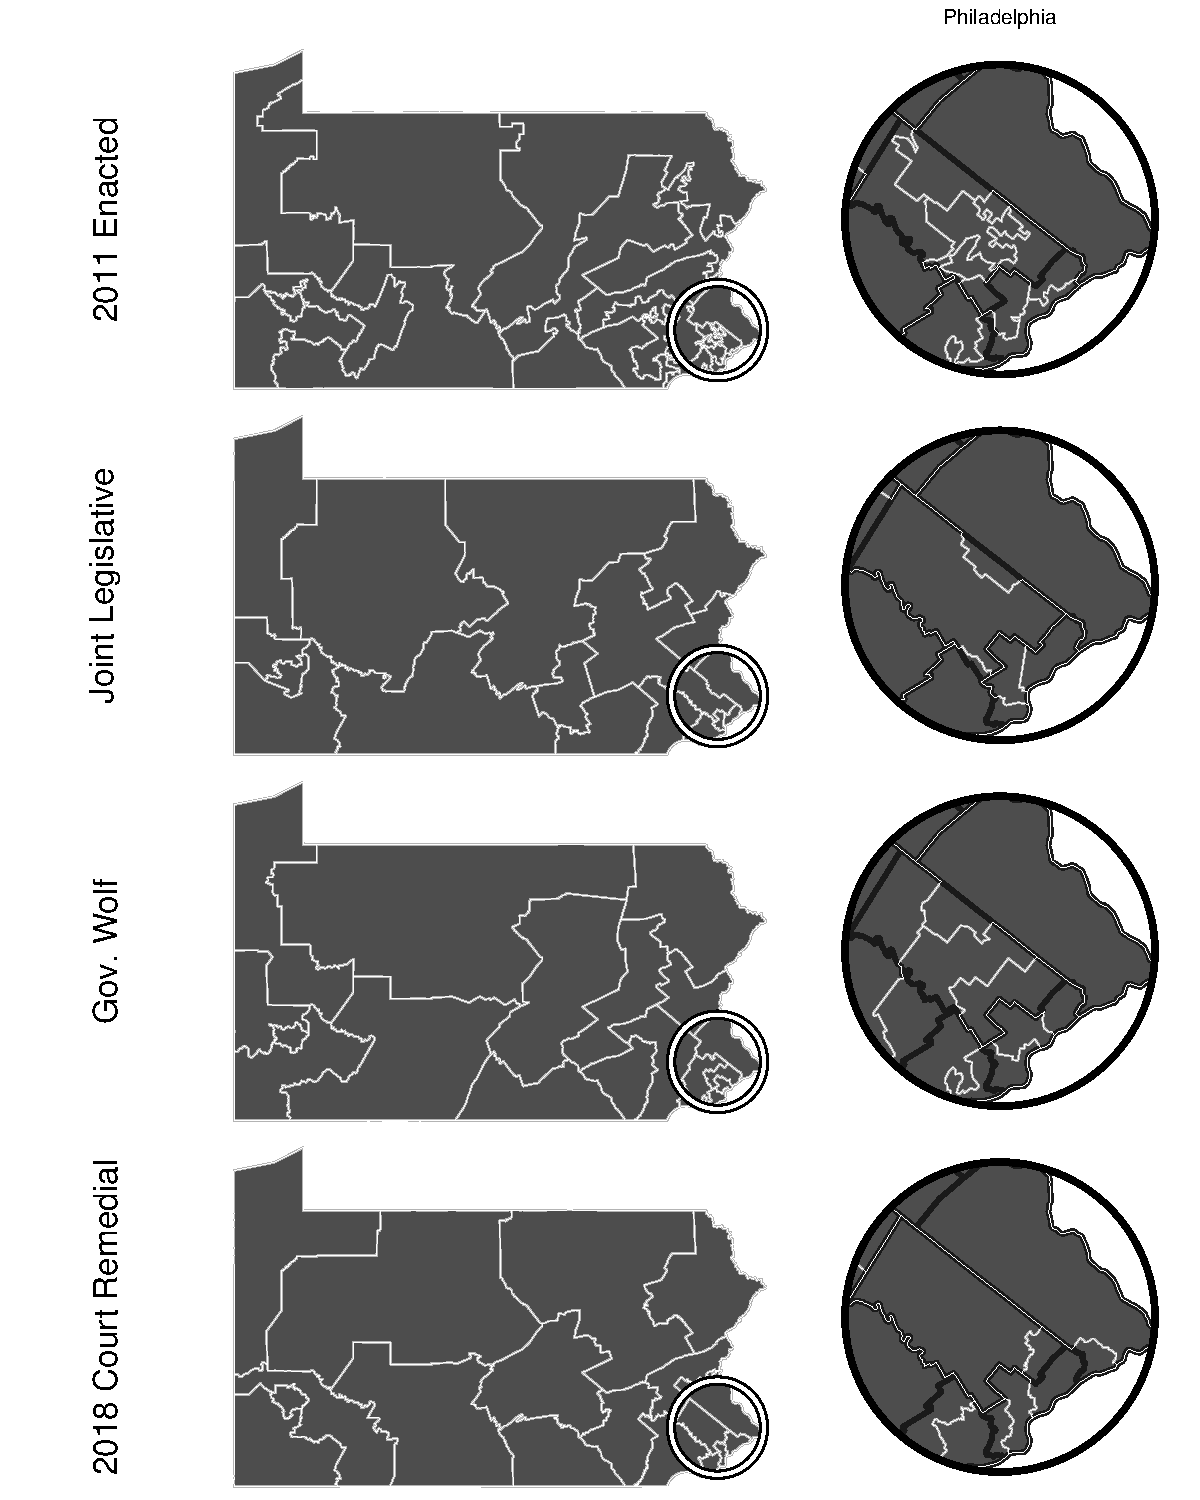
\includegraphics[width=1\textwidth,height=\textheight]{Figures/fig_maps.pdf}
\caption{Maps Of The Proposed Pennsylvania Congressional
Districts{}}\label{fig:maps}
}
\end{figure}

\tabnotes{Maps a drawn with a Mercator projection. Shapefiles were obtained from the Pennsylvania Supreme Court website for the four government plans.}

INSERT FIGURE \protect\hyperlink{fig:maps}{{[}fig:maps{]}} ABOUT HERE

\hypertarget{compactness}{%
\subsubsection*{Compactness}\label{compactness}}
\addcontentsline{toc}{subsubsection}{Compactness}

The measurement of compactness has long been a central issue in the
districting literature \citep[see
e.g.,][]{Reock1961, Niemi1990, Polsby1991, Webster2013, Kaufman2018}.
Indeed, the original gerrymander was assumed to be evidence of political
manipulation because of its irregular shape \citep{Martis2008}. Some
minimal level of compactness can make it harder to gerrymander \citep[
cf. \citet{Webster2013}]{Reock1961, Altman1998}. But compactness is not
a magic wand that rules out the possibility of political manipulation.
Moreover, as many authors have shown, compactness has multiple
dimensions, and these different dimensions need not move in parallel
with one another; thus a plan appears compact on one dimension might
appear ill-compact on another. The two most common ideas of compactness
refer, on the one hand, to how close a legislative district's boundaries
are to its geographic center and, on the other, to how ``regular'' in
shape a district appears to be \citep{Niemi1990, Kaufman2018}. In Table
\protect\hyperlink{tab:summaries}{{[}tab:summaries{]}} we report two
well-known measures which tap respectively each of these two dimensions.
The \emph{Polsby-Popper} measure looks at perimeter irregularity by
examining the area of the district compared to that of a circle with
similar perimeter, while the \emph{Reock} measure compares the area of a
district with that of the district's circumscribing circle
\citep{Reock1961, Polsby1991}. \footnote{\(A_D\) = area of district,
  \(P_D\)= perimeter of district, \(Circle_D\)= minimum circumscribing
  circle;\\
  \emph{POLSBYPOPPER} = \(\frac{4 \pi A_D}{{P_{D}}^{2}}\) \emph{REOCK} =
  \(\frac{A_D}{A(Circle_D)}\)}

The 2011 Enacted map looks awful by both compactness measures compared
to the Court-ordered map, or even compared to the two proposed remedial
maps; while both the Republican and the Democratic proposed remedial
maps look reasonable by both compactness measures, even though the
Democratic plan is superior to the Republican plan and the court-ordered
map is superior to both. However, until we examine the likely partisan
effects of these four plans we are not in a position to conclusively
rule out the possibility that one or more of the remedial plans is a
``\emph{stealth gerrymander}''. As is now well recognized,
gerrymandering can be found even in plans with compact appearing
districts, or in a plan with districts that preserve most county
borders.

Each of the three measures in Table
\protect\hyperlink{tab:summaries}{{[}tab:summaries{]}} indicates a very
dramatic deviation from good government standards in the 2011 Enacted
map. And, each of three metrics order the plans in good government terms
from worst to best in exactly the same way, with the worst plan being
the 2011 Enacted map, the next worst being the Republican remedy plan,
followed by the the Democratic remedy plan, and the very best being the
court-ordered map. Moreover, as we will see later, the same ordering of
plans is reflected when we examine the partisan implications of the
various maps, with the map ordered into place as a remedy by the
Pennsylvania Supreme Court close to perfectly neutral in its expected
partisan effects once we recognize the implications of the partisan
geography in Pennsylvania in ``naturally'' tilting outcomes slightly in
a pro-Republican direction because of differences in the degree of
geographic concentration of each party's supporters (see below).
Moreover, we show that the proposed Republican remedy plan can be
characterized as a ``disguised'' pro-Republican partisan gerrymander --
what we call a ``stealth gerrymander'' -- which is nearly as pernicious
in its expected pro-Republican partisan consequences as the 2011 plan
whose effects it claims to ``remedy''.

To give a more intuitive feel for how egregiously ill-compact the 2011
map is compared to the other alternatives we are considering, Figure
\protect\hyperlink{fig:maps}{{[}fig:maps{]}} shows all four maps in the
same scale, in a gray and white format. What is visually apparent from
these maps is how aesthetically ``ugly'' the 2011 map is compared to all
of its alternatives. But it also clear that three remedy maps that are
similar in having relatively few county cuts nonetheless can look quite
different in terms of how each configures districts. \footnote{This
  latter point is reinforced if we examine good government maps prepared
  by
  \href{https://www.dailykos.com/stories/2018/2/8/1739648/-Pennsylvania-will-soon-redraw-its-House-map-to-end-GOP-gerrymandering-How-would-you-draw-the-lines}{DailyKos}
  and by the present authors (available upon request).}

\hypertarget{asymmetry-measures}{%
\subsection*{Asymmetry Measures}\label{asymmetry-measures}}
\addcontentsline{toc}{subsection}{Asymmetry Measures}

We emphasize that a partisan gerrymandering claim based on statewide
political consequences should also provide evidence that the (a)
gerrymandering indicators that are found cannot be explained simply by
the geographic distribution of each party's electoral support (e.g.,
differential concentration of electoral support can lead to what has
been called a ``natural gerrymander''), and (b) that the partisan
asymmetry in translating votes into seats is not due to chance alone
(e.g., many highly competitive seats won by very narrow margins) but can
be expected to be durable. With only 18 districts, sensitivity to chance
effects is particularly important.

Rebuttal to any claims that the partisan asymmetries observed in the
consistent outcomes of the 2011 map can be attributed primarily to
differential concentration of party voting strengths, or to chance, is
found in the expert witness testimony in the case (see esp.~the
simulations of potential good government maps done by Professor Chen,
discussed in detail in the Pennsylvania Supreme Court opinion in the
case, and on which the Court placed great reliance). With respect to the
durability of the effects of the 2011 map, this plan yielded unchanged
13R-5D results in all three elections where the map was used. To help
explain this over time consistency we note that the 2011 Map has
primarily safe seats (13 of 18 won with greater than a 10 percentage
point margin). But, indicative of the pro-Republican gerrymander
achieved with the 2011 map, those safe seats are distributed in a highly
asymmetric fashion, with nine essentially safe seats for Republicans and
only four for Democrats. \footnote{However, we should note that some
  authors \citep[e.g.,][]{Grofman2019_ELJ} have argued that a partisan
  gerrymandering claim at a jurisdiction-wide level must also be
  reinforced by district specific evidence of manipulation of particular
  district boundaries. As noted earlier, we do not discuss this type of
  district specific evidence here, other than to point out that such
  evidence was presented at the trial, and that this evidence was used
  to support the Court's finding that the Pennsylvania congressional map
  was an unconstitutional gerrymander under Pennsylvania state law.}

There are several metrics that have been proposed to look at the degree
to which there is asymmetry in seats-votes relationships that might be
indicative of partisan gerrymandering: (1) \emph{partisan bias}
\citep{Tufte1973}, (2) the \emph{mean-minus-median} gap
\citep{Mcdonald_Best_2015_ELJ} (3) the \emph{efficiency gap}
\citep{Stephanopoulos2014_UofChicagoLaw}, and most recently (4)
\emph{declination} \citep{Warrington2018}. Each of these measures can be
directly calculated for the 2011 map based on district election outcomes
in 2012, 2014, and 2016. \footnote{Another recently proposed measure is
  a simplified version of partisan bias which lacks the advantage of
  separately calculating bias and responsiveness (swing ratio). It is
  calculated by taking the average two-party vote for the dominant party
  and adjusting it uniformly downward in each district so that the two
  parties receive exactly 50\% of the overall vote; then we look to see
  how far the seat share the dominant party now receives is from 50\%
  \citep{Wang2016_SLR}.} values favor Republicans, while values favor
Democrats.

We now define these four measures of gerrymandering in which we will
evaluate the four competing maps.

\hypertarget{partisan-bias}{%
\subsubsection*{Partisan Bias}\label{partisan-bias}}
\addcontentsline{toc}{subsubsection}{Partisan Bias}

\emph{Partisan Bias} indicates asymmetry in the translation of each
party's votes into seats. Customarily, partisan bias is measured at the
(hypothetical) point where each party's share of the two-party vote is
exactly 50\%. At that point, both parties should, by symmetry, receive
identical seats shares. Thus, the difference between a party's projected
seat-share with 50\% of the vote and exactly 50\% can be taken as a
measure of partisan bias. Note, however, that although a plan must be
proportional at the (\(50,50\)) point, a partisan bias of zero does
imply proportional representational. What partisan bias taps is the
differential treatment of parties. Thus, for example, if party R gets
61\% of the seats with 52\% of the vote, this is not a sign of bias as
long as party L also can be expected to get 61\% of the seats were it to
have 52\% of the vote. \footnote{Although the basic idea goes back at
  least as far as \citet{Dahl1956}, the modern \emph{locus classicus} in
  political science for the idea of partisan bias (and the parallel
  concept of responsiveness/swing ratio) is \citet{Tufte1973}, with
  important recent work done by Gary King (see e.g.,
  \citep{GelmanKing1994_unifiedAJPS}; and reviewed in
  \citet{GrofmanKing2007_ELJ}). A closely related line of research is
  found in the political geography literature (with \emph{locus
  classicus} \citeauthor{Brookes1959}
  \citetext{\citeyear{Brookes1959}; \citealp{Brookes1960}} -- with some
  further methodological improvements by scholars such as
  \citeauthor{Johnston1994}
  \citetext{\citeyear{Johnston1994}; \citealp{Rossiter1997}}, and
  \citet{Johnston2002}.}

There are a number of different ways to estimate partisan bias based on
the shape of the votes to seats distribution
\citep{Tufte1973, Grofman1983, Browning_King_1987_seats_votes, GelmanKing1994_unifiedAJPS, Grofman_et_al_1997_SwingRatio_Bias, Zingher2016_bias_swingratio_JEPP}.
The method we use here is that of \citet{Tufte1973}. Hypothetical
elections are constructed by incrementally adding (or subtracting) one
percentage point (on average) at a time to find aggregate seat outcomes
under differing mean vote shares. The resulting (\(s\), \(v\)) points on
the votes-to-seats curve are then converted to a log odds form by using
\(log(\frac{s}{1-s})\) as the dependent variable, and
\(log(\frac{v}{1-v})\) as the independent variable. A regression on the
transformed variables is then run, with transformed \(s\) as the
dependent variable, for \(v\) values in some range near a 50\% vote
share. \footnote{Where to center the \emph{seats/votes} curve is an
  unresolved issue in the literature. In
  \citet{GelmanKing1994_unifiedAJPS} \texttt{JudgeIt} program, the
  choice is to center the election at the average Democratic vote share
  over recent elections. \citet{Kastellec_et_al_2008_PS} similarly
  simulates data for average vote shares between 45\% and 55\%. We
  checked for consistency between the methods by running the numbers in
  three ways: centering the simulated outcomes at an average election
  vote share, centering the simulated outcomes at a tied 50/50 election,
  and centering the simulated outcomes at the actual election results in
  the particular election. All three variations provide similar
  estimates, as do the results from \texttt{JudgeIt}. Readers should
  note that, with only 18 districts, too much weight should not be
  placed on the exact bias coefficients reported {[}see the discussion
  in \citet{Browning_King_1987_seats_votes}{]}; but the relative
  magnitude of the bias values across the different plans is fully
  congruent with the evaluations of probable partisan gerrymandering
  yielded by the other measures. Because of the limited number of
  districts in the plans, the same caution is urged for all the measures
  of gerrymandering reported in this essay. We have devoted more space
  to partisan bias than to the other measures of gerrymandering reported
  in this essay due to it's complexity than to the other more
  straightforward measures.} \emph{Partisan Bias} is then calculated
from the intercept of this regression using an exponential
transformation (for details see \citet{Grofman1983}).

\hypertarget{mean-median-gap}{%
\subsubsection*{Mean-Median Gap}\label{mean-median-gap}}
\addcontentsline{toc}{subsubsection}{Mean-Median Gap}

When districts are sorted according to two-party vote share, the
\emph{Mean-Median Gap} is the difference between the average vote
percentage for a party and its vote share in the median district
\citep[see][]{Best2018}. This measure is a variant of \emph{skewness}.
When the mean is substantially higher or lower than the median, this is
taken to be indicative of partisan bias.

\hypertarget{efficiency-gap}{%
\subsubsection*{Efficiency Gap}\label{efficiency-gap}}
\addcontentsline{toc}{subsubsection}{Efficiency Gap}

The \emph{Efficiency Gap} is calculated as defined in
\citet{Stephanopoulos2014_UofChicagoLaw}, where all the party's votes
are wasted if they lose the district, and all the winner's votes over
50\% are wasted. The difference between each party's wasted votes is
then divided by the total votes cast to produce the \emph{efficiency
gap}, with a value of zero denoting what is regarded as ideal. As noted
in \citet[p.~13]{Best2018}, this is equivalent to taking an aggregate
responsiveness (swing ratio) of two as ideal.

\hypertarget{declination}{%
\subsubsection*{Declination}\label{declination}}
\addcontentsline{toc}{subsubsection}{Declination}

Among the more recent measures of gerrymandering is the
\emph{Declination}. \emph{Declination} is an astronomical term referring
to the angle on a compass, with a Latin root meaning ``a bending away''.
For gerrymandering, it uses the angles created from ordering all of the
districts by vote share, computing the mean vote-share for each party
separately for the seats they won, and then comparing the differences in
their distribution. To compare, a line is draw from the mean vote-share
to the 0.5 line separately for each party. The angle formed from the
different slopes of the line is called the \emph{declination}. An angle
indicates whether a plan is a gerrymandering, under the logic that
vote-shares should be distributed in some uniform manner across
districts. If partisan are \emph{packed}, the angle will be greater. All
values range between -1 and 1. Though we have defined the vote-share in
terms of Republican outcomes, we adjusted the values such that values
are favorable to the Democrats. Further information on declination can
be found in \citet{Warrington2018}.

In our view, none of these four measures standing alone can be taken to
be proof of gerrymandering. Rather we see them as potentially
reinforcing indicators. Our own analyses have found hypotheticals where
these measures can generate either a false positive or a false negative,
but we have also found that consistent bias in the same direction is
unlikely when we use multiple indicators (data omitted for space
reasons). We will return to a discussion of the results later in this
essay. Here we point out, however, all four indicators point clearly and
overwhelmingly in the same direction vis-à-vis the 2011 Enacted plan --
namely that it is a blatant pro-Republican partisan gerrymander.

\hypertarget{evaluation-of-the-2011-enacted-map}{%
\subsection*{Evaluation of the 2011 enacted
map}\label{evaluation-of-the-2011-enacted-map}}
\addcontentsline{toc}{subsection}{Evaluation of the 2011 enacted map}

\hypertarget{partisan-results-in-actual-congressional-elections-held-under-the-2011-map}{%
\subsubsection*{Partisan results in actual congressional elections held
under the 2011
map}\label{partisan-results-in-actual-congressional-elections-held-under-the-2011-map}}
\addcontentsline{toc}{subsubsection}{Partisan results in actual
congressional elections held under the 2011 map}

The best evidence about a plan's partisan consequences is, of course,
evidence derived from actual elections under the plan -- if there are
any -- though we do need to check if there are highly anomalous aspects
to one or more of these elections which would make results from them
hard to generalize. Also, the existence of incumbency advantage can have
a distorting effect on the translation of votes into seats, since
incumbents may deter strong challengers, thus reducing the vote-share of
the minority party \citep{Jacobson_Kernell_1981, Abramowitz1991}.
Nonetheless, simply from examining outcomes in the three elections held
under the plan (2012, 2014, 2016), the claim that the 2011 Pennsylvania
congressional plan is an egregious partisan gerrymander is very hard to
refute since (a) regardless of voter preferences the plan returned 13
Republicans and 5 Democrats, with no district changing hands over the
course of the three elections, and (b) in those three elections,
Democrats won only 28\% of the seats (5 out of 18), despite winning a
substantial share of the vote in all three elections. In 2012, the
Democratic share of the average two-party vote in the congressional
elections in Pennsylvania was 48.0\%, in 2014 it was 44.5\%, and in 2016
it was 45.8\%. \footnote{For consistency, we report the average vote
  share after imputing 0.25 and 0.75 for uncontested districts. In raw
  votes, Democrats won more votes than Republicans in 2012, and the
  difference is an artifact of the plan's `packing' and `cracking'. The
  Democratic raw vote shares are 50.8\% in 2012, 44.5\% in 2014, and
  45.9\% in 2016.} Thus, the discrepancy between Republican vote share
and Republican seat share was huge, and yet the seat share appeared to
be immutable. Table \protect\hyperlink{tab:congsum}{{[}tab:congsum{]}}
shows the indicators of statewide partisan gerrymandering effects that
provides additional compelling evidence of the 2011 map as an (enduring)
partisan gerrymander.

\centering

2012 2014 2016 AVE ------------------ ------------ ------------
------------ ------------

{[}-1.8ex{]} Seats {[}13R-5D{]} {[}13R-5D{]} {[}13R-5D{]} {[}13R-5D{]}
Seat \% 72.2\% 72.2\% 72.2\% 72.0\% Votes 51.1\% 55.5\% 54.2\% 53.3\%
Bias 0.13 0.1 0.11 0.11 Efficiency Gap 0.21 0.11 0.17 0.16 Mean/Median
0.06 0.06 0.06 0.06 Declination 0.46 0.36 0.39 0.4

: U.S. House Election Summaries\\
(PA 2012-2016 Enacted Map){}

\tabnotes{Calculations based on actual congressional elections in Pennsylvania under the map found unconstitutional in 2018. Uncontested races are imputed with 0.25 and 0.75 for the respective winners. Un-adjusted Republican two-party vote totals are 49.2\% for 2012, 55.5\% for 2014, and 54.1\% for 2016. All votes are calculated from the Republican perspective of the two-party vote. We've adjusted all gerrymandering measures such that negative numbers indicate bias in favor of the Democrats.}

\textbf{INSERT TABLE \protect\hyperlink{tab:congsum}{{[}tab:congsum{]}}
ABOUT HERE}

\hypertarget{evaluating-district-plans-using-statewide-elections-to-provide-a-normal-vote-baseline}{%
\subsection*{Evaluating district plans using Statewide elections to
provide a normal vote
baseline}\label{evaluating-district-plans-using-statewide-elections-to-provide-a-normal-vote-baseline}}
\addcontentsline{toc}{subsection}{Evaluating district plans using
Statewide elections to provide a normal vote baseline}

In order to assess expected partisan consequences for plans that have
not yet been implemented we need to develop a predictive equation, and
one such way is with data on partisan outcomes for state-wide elections
projected into the new districts. For example, Professor Jowei Chen in
his testimony in the Pennsylvania case used a composite of the six
state-wide elections between 2008 and 2010 to estimate the political
consequences of alternative maps. After extensive investigation of
alternative prediction models and their accuracy in reproducing the
partisan outcomes of the 2012, 2014, and 2016 congressional elections at
the district level (data omitted for space reasons), we have opted for a
model that takes the average of five state-wide 2016 elections that
reflect a balance of Republican and Democratic success: President, U.S.
Senate, PA Attorney General, PA Treasurer, and PA Auditor. \footnote{We
  use the five-election composite to calculate all four plans. We
  aggregate voting district level (precincts) data for these five
  statewide elections and project them to the three maps in which we are
  comparing the 2011 enacted map.} Republicans won the statewide vote in
two of them (President, U.S. Senate), while the Democrats won the
statewide vote in three of them (Auditor, Treasurer, and Attorney
General). The average vote for the Republicans across these five
elections was 49.1\%. \footnote{We report the Republican share of the
  two-party vote (\(\delta_{i}\)). Districting plans are represented by
  \(\mathcal D\), (e.g., \(\mathcal D_{enacted}\),
  \(\mathcal D_{remedial}\), \ldots{}, \(\mathcal D_{j}\)), and each
  election in year \(y\) has a district vote distribution
  \(\Delta_{y} = [\delta_{y1}, \delta_{y2}, \dots, \delta_{yi}]\). To
  find the overall state-wide vote share, we calculate the average
  district vote share,
  \(\bar{\Delta}_{\mathcal D y} = \frac{1}{n}\sum\limits_{i=1}^{n} \delta_{yi}\).
  By averaging, we reduce the influence of turnout variation among
  districts. This district-specific average is a useful state-wide
  estimate of voter sentiment though it is in part effected by the
  particular configuration of districts being examined \citep[see e.g.][
  cf.
  \citep{Grofman_et_al_1997__IntedgratedPerspective_ES}]{Kastellec_et_al_2008_PS}.
  In particular, incumbency advantage effects affect our ability to
  accurately predict vote outcomes. In ancillary work not reported here,
  we have looked at changes in congressional incumbency advantage in
  Pennsylvania over multiple decades \citep[cf.][]{Jacobson2015}. We
  compiled the composite measure using both the sum of the raw votes by
  party and an average of the two-party vote in the five races at the
  district level (see discussion on alternative ways to tabulate
  vote-shares in \citet{Grofman_et_al_1997__IntedgratedPerspective_ES}.
  Both ways result in the same district partisanship outcomes in all
  plans.}

We need to check that our five-election composite offers a plausible
basis for a prediction model that accounts for the idiosyncrasies
inherent to congressional districts. Encouragingly, our five-election
composite results is the same 13R-5D result that the 2016 congressional
races delivered. Additionally, each district's outcome is identical to
the 2016 congressional district results, when we uniformly adjust in
each district the projected vote based on the composite state-wide
elections (the ``normal'' vote, without congressional incumbency
effects) by an amount equaling the difference between the statewide
legislative vote and the the statewide congressional vote.

When we look at the five election composite for the 2018 court remedial
plan, we need to (a) adjust it for the actual statewide congressional
Democratic vote share in 2018, and (b) to take into account this
differential incumbency advantage that still benefits Republicans.
Without doing so, the outcomes of the Court-ordered plan might have a
wide range, with anywhere from a 5R to an 11R outcome possible because
of the high number of competitive seats. However, when we take both
factors into account by uniformly shifting the state-wide composite to
reflect the 2018 statewide two-party congressional vote, and by adding
in congressional incumbency advantage, which we have estimated in the
2012-2016 period to be on the order of magnitude of 4.3\% (analyses
omitted for space reasons), we get a 9R-9D outcome as the most likely
outcome in 2018 under the court-ordered map in our predictive model.
Thus, our confidence in the five election projection method is further
buttressed when we applied this method to predict the results of the
2018 election under the court-ordered remedial map in the light of the
actual statewide aggregate results in 2018, and taking incumbency
effects into account. In the congressional elections of 2018, the raw
Republican two-party vote share in 2018 was 44.8\%, which represented a
Democratic advantage, but not enough to overcome the twin barriers to a
Democratic majority of over-concentration of Democratic support in urban
areas and continued Republican incumbency advantage. \footnote{Six
  Republicans and five Democrats ran for re-election after the new map
  was put in place. No incumbent lost. There were two Republican
  incumbents who won by less than 2 percentage points, along with one
  who won by less than 3 percentage points. There was just one seat won
  by Democrats in 2018 with a margin of 5 percentage points or less.
  Republicans therefore had four incumbents running and winning in
  competitive districts compared to just two for Democrats (10+
  percentage point margin).} We are not claiming to predict vote shares
in advance of an election. We also recognize that the composite of
state-wide elections is intended to provide a ``normal vote'' baseline
that must be ``corrected'' with incumbency effects if we do wish to
actually predict outcomes.

We must distinguish our ability to assess asymmetry in expected
seats-vote relationships based on the ``normal vote'' distribution of
party support across districts -- and thus to assess the degree to which
a plan is a gerrymander -- from our ability to predict actual election
outcomes. The more competitive districts there are in a map, the more
results depend strongly on electoral tides, and the greater the
potential for winning vote margins in some districts to be small and
determined by factors idiosyncratic to a district and by incumbency
advantage. The 2011 map has 13 non-competitive districts (10+ percentage
point margin) with a clear 9-4 Republican advantage, thus virtually
guaranteeing continued Republican dominance regardless of aggregate two
party vote share. The Court drawn map, comparatively, had only 8
non-competitive districts, with a balance of 3-R and 5-D. Which party
will control the delegation under a highly competitive plan such as the
Court-ordered plan depends almost entirely on the state-wide vote share
and on incumbency advantage, along with idiosyncratic features of the
competitive districts that might be small in magnitude but still matter
in highly competitive seats.

We wish to do a further robustness check on the plausibility of using
our five-election composite to calculate the various metrics designed to
measure potential gerrymandering. One way to do this is to see how well
the composite (calculated at a hypothetical 50\% vote share) mimics the
results of the values for the four metrics for the 2011 map that we
previously obtained using the actual congressional election results for
that map. What we are doing is comparing a hypothetical ``normal vote''
\citep{Converse1966} assumption (based on a statewide vote in which we
are not taking incumbency effects into account) with the average of what
we actually get in three different congressional elections. The
congressional results for 2012-2016 and an average of the three,
reported in Table \protect\hyperlink{tab:congsum}{{[}tab:congsum{]}},
are 0.11 for partisan bias, 0.16 for the efficiency gap, 0.06 for the
value of the mean minus median gap, and 0.40 for \emph{declination}. The
comparable results from Table
\protect\hyperlink{tab:gerry}{{[}tab:gerry{]}} for the 2011 enacted map
at 50\% vote-share are 0.09, 0.24, 0.05, and 0.39. \footnote{If we
  center the simulations at the 2016 statewide Republican vote of 53.3\%
  of the vote, we again get remarkably consistent estimates {[}0.09,
  0.19, 0.05, 0.46{]}.}

\centering

2011 Enacted Joint Legislative Gov.~Wolf 2018 Court Remedial
-------------------------- ------------------ -------------------
------------------- ---------------------

{[}-1.8ex{]} Partisan Bias 0.09\(^{***}\) 0.08\(^{***}\) 0.06\(^{**}\)
0.04\(^{}\) \emph{{[}0.05, 0.13{]}} \emph{{[}0.03, 0.12{]}}
\emph{{[}0.02, 0.11{]}} \emph{{[}-0.01, 0.08{]}} Efficiency Gap
0.24\(^{***}\) 0.22\(^{**}\) 0.14\(^{}\) 0.08\(^{}\) \emph{{[}0.09,
0.36{]}} \emph{{[}0.07, 0.36{]}} \emph{{[}0, 0.3{]}} \emph{{[}-0.07,
0.21{]}} Mean/Median 0.05\(^{***}\) 0.04\(^{**}\) 0.04\(^{*}\)
0.02\(^{}\) \emph{{[}0.02, 0.07{]}} \emph{{[}0.01, 0.07{]}} \emph{{[}0,
0.07{]}} \emph{{[}-0.01, 0.05{]}} Declination 0.39\(^{**}\) 0.33\(^{*}\)
0.21\(^{}\) 0.14\(^{}\) \emph{{[}0.13, 0.63{]}} \emph{{[}0.07, 0.61{]}}
\emph{{[}-0.02, 0.47{]}} \emph{{[}-0.1, 0.42{]}}

: Measures of Gerrymandering for the Four Considered Plans at 50\% Vote
Share{}

\tabnotes{$^{*}$p $<$ 0.05; $^{**}$p $<$ .01; $^{***}$p $<$ 0.001. Measures are averages of 1,000 simulations for each map using the 2016 composite. Brackets numbers are the 95\% range.}

\textbf{INSERT TABLE \protect\hyperlink{tab:gerry}{{[}tab:gerry{]}}
ABOUT HERE}

The findings from Table \protect\hyperlink{tab:gerry}{{[}tab:gerry{]}}
are very clear; regardless of which metric we examine, the 2011 map is
the most gerrymandered. Not surprisingly, the nature of the bias is in a
pro-Republican direction. Given the cumulative weight of all the
evidence, the 2011 congressional map was clearly an egregious
pro-Republican gerrymander. All four measures of potential
gerrymandering are statistically significant for the 2011 map. In
contrast, as we might expect, the court-ordered plan, prepared by a
respected expert whose instructions were to satisfy good government
criteria, was by a considerable margin the closest to a perfectly
neutral plan in partisan terms according to all four measures. Indeed,
none of the four measures of potential gerrymandering is statistically
significant for the court-ordered map. And when we turn to the
Republican Joint Legislative plan we find that all four measures are
again statistically significant.

Finally, we return to the plan offered by the Democratic governor,
Governor Wolf. To our surprise, this plan appeared to have a
pro-Republican tilt, nearly to the same extent as the joint legislative
plan for three of the four metrics in Table
\protect\hyperlink{tab:gerry}{{[}tab:gerry{]}}. This puzzling finding
suggests that the Governor might have been under pressure from
Democratic incumbents not to reduce their expected vote margins, or that
he sincerely intended it to be a compromise that the Republican
legislature might agree to. However, as shown in
\protect\hyperlink{tab:gerry}{{[}tab:gerry{]}}, two of the apparent
pro-Republican indicators for the plan are statistically insignificant.
Moreover, there is one important difference between the joint plan and
that of the Governor: among the seven districts likely to be won by
Democrats, the Democratic percentages are cut more narrowly in the
Republican plan than in the Governor's plan in three of the districts so
that, in a good Republican year, Republicans will do better under their
plan than under the Democratic plan.

\centering

2011 Enacted Joint Legislative Gov.~Wolf 2018 Court Remedial
--------------------------------- ------------------------------
------------------------- -------------------------
------------------------------

\begin{verbatim}
 \[-1.8ex\] Mean Seat Share               12.2R-5.8D                  11.7R-6.3D                10.8R-7.2D                   10.2R-7.8D
                                 *\[10.8R-7.2D, 14.4R-3.6D\]*   *\[9R-9D, 14.4R-3.6D\]*   *\[9R-9D, 12.6R-5.4D\]*   *\[7.2R-10.8D, 12.6R-5.4D\]*
      Median Seat Share                     12R-6D                      12R-6D                    11R-7D                       10R-8D
\end{verbatim}

Probability Republican Majority 98.6\% 97.3\% 88.3\% 69.4\% Probability
Democratic Majority 0.3\% 0.3\% 2.0\% 6.6\% Probability Tied Delegation
1.1\% 2.4\% 9.7\% 24.0\%

: Probabilistic Projections of Partisan Outcomes for Four Plans at 50\%
Vote-Share{}

\tabnotes{Using a Composite of Five Statewide Elections (adjusted to a 50\% Vote Share) but not correcting for incumbency. We report the mean seat-share from 1,000 simulations, along with a 95\% range of the simulated outcomes.}

\textbf{INSERT TABLE \protect\hyperlink{tab:prob}{{[}tab:prob{]}} ABOUT
HERE}

Looking at the evidence above, we see exactly the same ordering of plans
according to their characterizability as a partisan gerrymander as we
saw when we ordered plans according to the degree to which they
satisfied good government criteria (see Table
\protect\hyperlink{tab:summaries}{{[}tab:summaries{]}}), with the 2011
map the worst and the 2018 court-ordered map far and away the best. This
conclusion is further buttressed by the data we present in Table
\protect\hyperlink{tab:prob}{{[}tab:prob{]}}. Here we create a
probabilistic simulation using statewide five-election composite (set to
a 50-50 vote share) to estimate the likelihood that random shocks (based
on past state inter-election shift data) would change party control of
the congressional delegation. We report the 95 percentile interval of
expect seat shares for each party when the vote is exactly tied 50-50.
\footnote{Simulations are conducted using a simple bootstrapping
  procedure where we uses the historic inter-election variability to add
  random noise to the composite results. An overview of this method can
  be found in \citet{Efron1979}.} The expectation is that at a tied
vote, when there is an even number of districts, that each party would
receive half the seats. This symmetric result is equivalent to a ``fair
plan''. In the court-remedial plan, we see a normal distribution of
expected seat-shares ranging from 7.2 to 12.6 Republican seats at 50\%
of the vote (Republicans are expected to gain at least 10 seats 69\% of
the time). For the Republican joint plan and the Democratic plan
submitted by Gov.~Wolf, the Democrats are virtually never expected to
have a majority of seats. Even in the Democratic plan, claimed by some
to be a pro-Democratic gerrymander, Democrats are only expected to
receive half or more of the seats 11.7\% of the time. In looking at the
unconstitutional gerrymander plan of 2011, Republicans are, except in
highly unlikely outliers, predicted to gain a majority (10+) seats, and
to win as many as 14/18 at of the vote! In our simulations of 1,000
potential election outcomes under the enacted 2011 map, 986 resulted in
at least ten Republican seats. The Republican remedial plan is not much
better, delivering ten plus seats for the Republicans in 973 of the
1,000 simulations. The Democratic plan improves slightly by limiting
Republican majorities to just 883/1,000 simulations, while the courts
map is the most fair with only 694 simulations resulting in an outright
majority for Republicans.

A number of analyses that come to conclusions similar to our own are
found in \citet{Nagle2019_ELJ}, an essay apparently written
simultaneously with this one. His work is a useful complement to this
one because much of it is concerned with alternative good government
maps and their properties. His primary concern is that voters are fairly
represented and that plans are responsive to voters. Nagle classifies
the 2011 map as a pro-Republican gerrymander and also finds the
Republican remedial map to be a ``stealth'' gerrymander. He additionally
agrees with our conclusion that, if there is any bias in the court plan
it is in a pro-Republican direction.

In the next section we introduce a potentially important distinction
between ``\emph{neutral plans}'' and ``\emph{fair plans}'', and we
consider some important aspects of Pennsylvania's electoral geography.

\hypertarget{natural-gerrymanders}{%
\subsection*{Natural Gerrymanders}\label{natural-gerrymanders}}
\addcontentsline{toc}{subsection}{Natural Gerrymanders}

In 2018, even under a court-drawn plan, in a year when Democrats had won
a clear majority of the aggregate two-party congressional vote,
Democrats only succeeded in winning exactly 50\% of the seats. Trying to
understand why evn plans not drawn by Republicans had some level of
pro-Republican bias requires us to look in more detail at the partisan
electoral geography of Pennsylvania. In Pennsylvania, Philadelphia is
overwhelmingly Democratic in voting. In particular, if you draw two
congressional districts entirely within Philadelphia County, one of them
is very likely to give Democratic candidates around 90\% of the vote,
and for sure, as long as both are wholly within the County, the average
vote in the two will be around 80\% Democratic no matter how you draw
the two districts. There are no other large, concentrated pockets of
equivalently overwhelmingly Republican voting strength. Thus, more
Democratic votes will \emph{naturally} be ``wasted'' in Philadelphia
than Republican votes will be ``wasted'' elsewhere in the state.
Additionally, the city of Philadelphia is landlocked, and its position
on the state's border reduces the ability of line drawers who favor
Democrats to distribute these voters into multiple districts so as to
minimize the extent to which Democratic votes in the county are wasted.
Additional Democratic wasted votes come in heavily Democratic Allegheny
County, the county in which the city of Pittsburgh is located. However,
saying that urban concentration of Democrats means that it is harder for
Democrats to turn their votes into seats than is the case for
Republicans does not mean that we cannot distinguish the effects of such
\emph{natural} gerrymanders from \emph{intentional} political
gerrymandering, since the latter generates perverse consequences for
Democratic voters to a far greater extent than the likely one district
or so penalty created by the nature of Pennsylvania's present electoral
geography. \footnote{\citet{Chen2013} estimate this bias as about 1.45
  seats (8\%) but Chen's expert witness testimony in the Pennsylvania
  cases generates a lower estimate of natural bias until one builds in
  the need to protect minority opportunity districts. Here, we need to
  be careful since the minority population in such districts in the
  enacted map may be larger than actually needed to assure effective
  minority representation, and the act of maintaining or even increasing
  high levels of minority population in the district may be a disguised
  way of packing Democratic voters so as to advantage the interests of
  the Republican party.} For example, in the first set of 500 map
simulations in his expert witness report, based only on traditional
redistricting criteria, but not including voting rights protections,
Professor Chen found that none resulted in the 13R-5D split as happened
in 2012 and subsequent years. The mode was 9R-9D. \footnote{Expert
  Witness Report, Jowei Chen (Pg. 15, 16, Figure 2).}

Recognizing the potential for so-called ``natural gerrymandering'', we
wish to highlight a potentially important distinction between
\emph{neutral} plans and \emph{fair} plans -- each of which reflects a
different approach to defining the baseline for what constitutes
gerrymandering. Neutral plans refer to those that are drawn entirely
with respect to traditional good government criteria, with no attention
paid to partisan considerations. One way to define partisan
gerrymandering is with respect to a baseline defined by the set of
feasible neutral plans -- and this was how one of the plaintiff's
experts in the Pennsylvania case, Professor Jowei Chen
\citep[cf.][]{Chen2015_JOP} shaped his testimony in the Pennsylvania
case, and in other cases in which he has testified. \footnote{Similarly,
  \citet{Grofman2018_ELJ} asserts that ``Gerrymandering occurs when a
  districting plan creates a disparate treatment of the vote share of
  the minority and majority voting blocs in a way that penalizes the
  minority in its ability to translate its voting support into seats
  compared to what we might expect from a plan drawn on the basis of
  neutral principles.''}

In contrast, we may wish to use the term ``fair'' as plans that
compensate for the difference in level of partisan concentration. Fair
plans do not seek to achieve proportional representation. Rather, they
aim to achieve partisan symmetry. A fair plan would yield a proportional
result when the vote shares are evenly split 50-50, but at points beyond
50-50, such as when party R wins 70\% of the districts with only 56\% of
the vote, party L can similarly win 70\% of the districts if it had
received 56\% of the vote. \footnote{\citet{Nagle2019_ELJ} views ``fair
  plans'' as the ideal, even if drawing a plan requires some degree of
  relaxing traditional and neutral criteria to accomplish symmetric
  maps.}

One clear finding of our analysis of the court-ordered map is that it
was drawn as a ``neutral map'', though not necessarily a ``fair map'' in
the sense we are using the term above. In order to create a truly ``fair
map'', in our view, it would have been necessary to break up
Philadelphia County in more than three pieces so as to avoid the natural
packing of Democratic voters. \footnote{Note that we certainly not
  advocating that such a three way split of Philadelphia should have
  been done.} But the Pennsylvania Supreme Court opted not to do that,
but to instead preserve county lines and draw a good government map. We
therefore identify the Court remedial plan as a ``neutral'' plan.

\hypertarget{conclusions-and-lessons-for-the-future-the-potential-impact-of-lwv}{%
\section{Conclusions and Lessons for the future; The Potential Impact of
LWV}\label{conclusions-and-lessons-for-the-future-the-potential-impact-of-lwv}}

While the Pennsylvania court opinion is limited to Pennsylvania, and
thus it might have seemed of importance only in Pennsylvania, in
footnote 71 of the Opinion (slip op. pp.~116-117), the court took what
we regard as a rather unusual step. It issued what can only be regarded
as an invitation to other state courts to use the same logic it used to
invalidate partisan gerrymanders in their own state. As we noted
earlier, the Court pointed out that there are twelve additional states
whose constitutions contain election clauses identical to the
Pennsylvania charter, requiring elections to be ``free and equal'':
Arizona, Arkansas, Delaware, Illinois, Indiana, Kentucky, Oklahoma,
Oregon, South Dakota, Tennessee, Washington, and Wyoming. \footnote{In
  its Opinion, the Court provided specific citations to each of these
  provisions which we have not reproduced.} However, only a handful of
these states are ripe for partisan gerrymandering challenges -- two are
single district states, several may not have unified control over the
districting process, some already have a commission drawing plans, and
in others, \emph{indicia} of gerrymandering are missing.

In looking to the future, we should also note that some states that are
generally regarded as among the most pernicious partisan gerrymanders,
Michigan, Ohio, North Carolina, Wisconsin are not included among the
twelve, nor is Maryland. On the other hand, we should also note that a
``free and equal'' elections clause is not the only avenue state courts
might use to attack partisan gerrymanders in the future. As University
of Kentucky College of Law Professor Joshua Douglas has pointed out,
virtually every state constitution protects voting rights more
explicitly than the U.S. Constitution does
\citep{Douglas2014_RightToVote}. In addition to the thirteen states that
require elections to be ``free and equal'', an additional thirteen have
state constitutional provisions that require elections to be ``free'' or
``free and open'', and these clauses could, in principle, be used in
exactly the same way as the ``free and equal'' clause. \footnote{We are
  indebted to Jonathan Lai of the Philadelphia Inquirer (personal
  communication, April 2018) for calling this information to our
  attention. These states include Colorado, Maryland, Massachusetts,
  Missouri, Montana, Nebraska, New Hampshire, New Mexico, North
  Carolina, South Carolina, Utah, Vermont, and Virginia \citep[ footnote
  86]{Douglas2014_RightToVote}. See a more detailed discussion in
  \citet{Elmendorf2018}.} Such clauses are found in some of the states
widely regarded as having the worst congressional plans, such as
Maryland and North Carolina.

Accordingly, some scholars have suggested turning away from the federal
judiciary altogether and instead focusing on state-level litigation
\citep[e.g.][]{Wang_et_al_2019_Labortories_UPJCL}. We believe that the
\emph{LWV} decision and the further comparative analyses of alternative
plans presented in the previous sections of this paper will help other
state courts navigate their way to decisions that strike down some
partisan gerrymanders as unconstitutional, while allowing others to
remain in place on the grounds that either they are not that severe, or
they are unlikely to be lasting in that they have sufficiently many
competitive seats as to be responsive to realistic changes in voting
patterns.

Now that litigation has been successful in state courts on the grounds
of egregious deviations from good government districting criteria, it
seems plausible that in the next wave of redistricting, mapmakers may
create covert gerrymanders like we've described in this essay. If so,
there remains the issue of whether state courts have the legal tools to
deal with these ``\emph{stealth gerrymander}''. \footnote{Commenting on
  the potential for the North Carolina district court to strike down
  their maps as unconstitutional (which ultimately they did), David
  Daley, author of ``Ratf**ked: Why Your Vote Doesn't Count''
  {[}\citet{Daley2016_ratf}**ked{]}, stated about a possible remedial
  plan by the map's original consultant that, ``{[}Thomas B. Hofeller{]}
  was really good at maps that look more normal, that break up fewer
  towns and counties but are just as partisan and just as advantageous
  for Republicans. It wouldn't surprise me at all if on a hard drive
  somewhere in Raleigh Tom Hofeller has another set of gifts for
  legislators.'' (as cited in \citet{Barnett2018_NC_gerry}). As we have
  pondered in this essay about Pennsylvania, the North Carolina court
  would have had to grapple with a plan which, according to traditional
  criteria, doesn't meet the standards of a gerrymander, but when
  looking at the partisan outcomes, clearly does. That a plan which was
  created which accomplished the partisan goals of the districters but
  also shielded itself from agitators by hiding the obvious indicators
  of gerrymandering was not enacted over one that makes obvious the
  intentions and thus potentially vulnerable to litigation is beyond the
  current authors' imagination.}

According to all four measures, the joint legislative plan offered by
Republican leaders is nearly as much a gerrymandered map -- in a
pro-Republican direction -- as is the 2011 map. As noted above, we
believe it appropriate to label this plan as a \emph{stealth
gerrymander} since it creates partisan asymmetries while (mostly)
providing the visual appearance of a good government map (see Figure
\protect\hyperlink{fig:maps}{{[}fig:maps{]}}). However, having labeled
the joint legislative plan a \emph{stealth gerrymander}, it is worth
reminding readers of two important points.

First, had this plan been the original plan adopted by Republicans, it
is very much an open question as to whether it would have been rejected
by the Pennsylvania Supreme Court. Even though, in partisan terms, it is
nearly identical to the 2011 plan, it is considerably more consistent
with good government criteria (see Table
\protect\hyperlink{tab:summaries}{{[}tab:summaries{]}}) -- not that much
worse than the Court Remedial plan -- that it would have required
detailed political election analyses like those we have done here to
demonstrate its \emph{stealth gerrymander} features, plus a court
willing to rule on political grounds, rather than good government
grounds that it was unconstitutional. Second, because the joint
legislative plan was not passed by the State of Pennsylvania's
legislature, the Court felt no need for particular deference to it (or
to the Governor's plan, for that matter). Thus, the Court was not bound
by the normal supposition with respect to districting that a plan
authorized by the state need not be the ``best possible'', but only
constitutional. That ``deference'' to legislative judgments and the
criteria they reflect, might well have tipped the balance toward
acceptance of the Republican joint legislative plan were it offered as
having been fully sanctioned by the State of Pennsylvania (the duly
elected legislature and Governor). \footnote{The Court picked the plan
  among those before it that most closely satisfied good government
  criteria -- which happily, thanks to Professor Persily's expertise as
  consultant to the Court, turned out to be its own plan, and thus a
  plan which the Court could know with certainty was not intended as a
  partisan gerrymander for either party. Whether it would have still
  sought to maximize compliance with good government criteria had the
  plan which did so been a ``stealth gerrymander'' is not a question we
  can answer.}

On the other hand, in the presence of this \emph{stealth gerrymander}
rather than the blatant gerrymander that came before it, the
Pennsylvania Court might well have relied on partisan impact evidence to
reach a conclusion of unconstitutionality. The language of the Final
Order implementing the Court's own plan strongly suggests this
possibility. There, the Court said about the 2011 plan that it

\begin{quote}
``was designed to dilute the votes of those who in prior elections voted
for the party not in power in order to give the party in power a lasting
electoral advantage. In stark contrast, Article I, Section 5 of the
Pennsylvania Constitution provides: `Elections shall be free and equal;
and no power, civil or military, shall at any time interfere to prevent
the free exercise of the right of suffrage.' Pa. Const. art. I, § 5. On
this record, it is clear that the 2011 Plan violates Article I, Section
5, since a diluted vote is not an equal vote'' (slip op. p.~2).
\end{quote}

Thus, we have some optimism that state courts can provide a venue to
check partisan gerrymandering, even when it comes in the form of a
\emph{stealth gerrymander}. But we have also placed a number of caveats
on any claim that state courts can compensate fully for any continued
failure of the federal courts to act. Citizen-based reforms such as
referendum and initiatives may also help with reducing egregious
gerrymandering in states where the passage of such measures is feasible.
\footnote{Since the U.S. Supreme Court's remand of the \emph{Gill} case
  in June 2018, Colorado, Michigan, Missouri, and Utah all passed ballot
  initiatives taking control of redistricting away from legislatures and
  given them to independent commissions. Six other states had, in the
  past several decades, adopted independent commissions: Alaska,
  Arizona, California, Idaho, Montana, and Washington. While some
  reformers see this as an excellent alternative to litigation,
  University of California Irvine Law Professor Rick Hasen
  (\href{https://blog.harvardlawreview.org/the-next-threat-to-redistricting-reform/}{Harvard
  Law Review -- The Next Threat to Redistricting Reform}) argues that
  the U.S. Supreme Court might, in the near future, disallow such
  commissions as unconstitutional when they involve congressional
  districting. Hasen's argument turns on the explicit language of the
  Constitution (``The Times, Places and Manner of holding Elections for
  Senators and Representatives, shall be prescribed in each State by the
  Legislature thereof; but the Congress may at any time by Law make or
  alter such Regulations, except as to the Places of chusing {[}sic{]}
  Senators.''), and the views of Justice Roberts in the Arizona
  Independent Commission case. On the other hand, forbidding
  redistricting commissions would call into question popular sovereignty
  and the right of the people to place checks on the legislature. H.R.1,
  introduced on the first day of the new legislative session after
  Democrats took control of the House of Representatives in what is
  widely viewed as a rebuke of President Trump's first two years in
  office, takes advantage of the constitutional provision allowing for
  Congress to make or alter the manner of elections by explicitly
  allowing for independent commissions in apparent anticipation of
  future litigation. It has passed the U.S. House of Representatives,
  but action has not been taken by a Republican majority U.S. Senate
  (circa June 2019).} Ultimately, there is no substitute for a federal
standard that guarantees each citizen in the United States \emph{equal
protection under the law}. Absent the United States Supreme Court
setting this standard, state courts offer one promising pathway towards
ending undemocratic partisan gerrymandering.

\clearpage
\nolinenumbers
\newgeometry{
        top=1in,
        bottom=1in,
        inner=0.85in,
        outer=0.85in,
        ignorehead,
        ignorefoot,
        nomarginpar,
    }

2

Automatically generated by Mendeley Desktop 1.19.4 Any changes to this
file will be lost if it is regenerated by Mendeley.

BibTeX export options can be customized via Preferences -\textgreater{}
BibTeX in Mendeley Desktop

\citet{article}\{GelmenKing1990\_inc\_AJPS, abstract = \{In this paper
we prove theoretically and demonstrate empirically that all existing
measures of incumbency advantage in the congressional elections
literature are biased or inconsistent. We then provide an unbiased
estimator based on a very simple linear regression model. We apply this
new method to congressional elections since 1900, providing the first
evidence of a positive incumbency advantage in the first half of the
century.\}, author = \{Gelman, Andrew and King, Gary\}, file =
\{:Users/cervas/Documents/Mendeley Desktop/Gelman,
King\{\_\}1990\{\_\}Estimating Incumbency Advantage Without
Bias.pdf:pdf\}, journal = \{American Journal of Political Science\},
month = \{nov\}, pages =
\{1142\{\{\}\(\backslash\)textendash\{\}\}1164\}, title = \{\{Estimating
Incumbency Advantage Without Bias\}\}, volume = \{34\}, year = \{1990\}
\} \citet{article}\{Colantoni2017, author = \{Colantoni, Claude S. and
Levesque, Terrence J. and Ordeshook, Peter C.\}, file =
\{:Users/cervas/Documents/Mendeley Desktop/Colantoni, Levesque,
Ordeshook\{\_\}1975\{\_\}Campaign Resource Allocations Under the
Electoral College.pdf:pdf\}, journal = \{American Political Science
Review\}, number = \{1\}, pages = \{141--154\}, title = \{\{Campaign
Resource Allocations Under the Electoral College\}\}, volume = \{69\},
year = \{1975\} \} \citet{article}\{Tufte1975, abstract = \{An
explanatory model for the outcomes of midterm congressional elections is
developed. Midterms are a referendum on the performance of the President
and his administration's management of the economy. The explanatory
model of midterm congressional elections is sufficiently powerful so as
to yield honest and accurate pre-election predictions of the national
two-party vote in midterm elections. These predictions have usually
outperformed pre-election forecasts based on survey data. The model is
extended by considering the translation of votes into seats, models of
the electorate as a whole and of the individual voter, and the causes of
the off-year loss by the President's party.\}, author = \{Tufte, Edward
R.\}, doi = \{10.2307/1958391\}, file =
\{:Users/cervas/Documents/Mendeley
Desktop/Tufte\{\_\}1975\{\_\}Determinants of the Outcomes of Midterm
Congressional Elections.pdf:pdf\}, issn = \{0003-0554\}, journal =
\{American Political Science Review\}, month = \{sep\}, number = \{03\},
pages = \{812--826\}, title = \{\{Determinants of the Outcomes of
Midterm Congressional Elections\}\}, url =
\{http://www.journals.cambridge.org/abstract\{\_\}S0003055400243645\},
volume = \{69\}, year = \{1975\} \} \citet{article}\{Polsby1991, author
= \{Polsby, Daniel D. and Popper, Robert D.\}, file =
\{:Users/cervas/Documents/Mendeley Desktop/Polsby,
Popper\{\_\}1991\{\_\}The Third Criterion Compactness as a Procedural
Safeguard Against Partisan Gerrymandering.pdf:pdf\}, journal = \{Yale
Law \{\&\} Policy Review\}, number = \{6\}, pages = \{301----353\},
title = \{\{The Third Criterion: Compactness as a Procedural Safeguard
Against Partisan Gerrymandering\}\}, url =
\{http://digitalcommons.law.yale.edu/ylprhttp://digitalcommons.law.yale.edu/ylpr/vol9/iss2/6\},
volume = \{9\}, year = \{1991\} \} \citet{article}\{Blackwell2017,
abstract = \{Journal of the American Statistical Association ISSN:
0162-1459 (Print) 1537-274X (Online) Journal homepage:
http://amstat.tandfonline.com/loi/uasa20 ABSTRACT In democratic
countries, voting is one of the most important ways for citizens to
influence policy and hold their representatives accountable. And yet, in
the United States and many other countries, rates of voter turnout are
alarmingly low. Every election cycle, mobilization efforts encourage
citizens to vote and ensure that elections reflect the true will of the
people. To establish the most effective way of encouraging voter
turnout, this article seeks to differentiate between (1) the synergy
hypothesis that multiple instances of voter contact increase the
effectiveness of a single form of contact, and (2) the diminishing
returns hypothesis that multiple instances of contact are less effective
or even counterproductive. Remarkably, previous stud-ies have been
unable to compare these hypotheses because extant approaches to
analyzing experiments with noncompliance cannot speak to questions of
causal interaction. I resolve this impasse by extending the traditional
instrumental variables framework to accommodate multiple
treatment--instrument pairs, which allows for the estimation of
conditional and interaction effects to adjudicate between synergy and
dimin-ishing returns. The analysis of two voter mobilization field
experiments provides the first evidence of dimin-ishing returns to
follow-up contact and a cautionary tale about experimental design for
these quantities. Supplementary materials for this article are available
online.\}, author = \{Blackwell, Matthew\}, doi =
\{10.1080/01621459.2016.1246363\}, file =
\{:Users/cervas/Documents/Mendeley
Desktop/Blackwell\{\_\}2017\{\_\}Instrumental Variable Methods for
Conditional Effects and Causal Interaction in Voter Mobilization
Experiments.pdf:pdf\}, issn = \{1537274X\}, journal = \{Journal of the
American Statistical Association\}, keywords = \{Causal
inference,Factorial design,Instrumental variables,Interaction,Voter
mobilization\}, number = \{518\}, pages = \{590--599\}, publisher =
\{Taylor \{\&\} Francis\}, title = \{\{Instrumental Variable Methods for
Conditional Effects and Causal Interaction in Voter Mobilization
Experiments\}\}, url =
\{https://doi.org/10.1080/01621459.2016.1246363\}, volume = \{112\},
year = \{2017\} \} \citet{article}\{Berlinski2007, abstract = \{We
analyse the determinants of ministerial hazard rates in Britain from
1945 to 1997. We focus on three sets of attributes (i) personal
characteristics of the minister; (ii) political characteristics of the
minister; and (iii) characteristics pertaining to the government in
which the minister serves. We find that educational background increases
ministers' capacity to survive, that female ministers have lower hazard
rates and older ministers have higher hazard rates. Experienced
ministers have higher hazard rates than newly appointed ministers.
Ministerial rank increases a minister's capacity to survive, with full
cabinet members having the lowest hazard rates in our sample.We use
different strategies to control for the characteristics of the
government the minister serves in. Our results are robust to any of
these controls.\}, author = \{Berlinski, Samuel and Dewan, Torun and
Dowding, Keith\}, doi = \{10.1017/S0007123407000129\}, issn =
\{0007-1234\}, journal = \{British Journal of Political Science\}, month
= \{apr\}, number = \{02\}, pages = \{245\}, publisher = \{Cambridge
University Press\}, title = \{\{The Length of Ministerial Tenure in the
United Kingdom, 1945--97\}\}, url =
\{http://www.journals.cambridge.org/abstract\{\_\}S0007123407000129\},
volume = \{37\}, year = \{2007\} \} \citet{article}\{Best2018, author =
\{Best, Robin E. and Donahue, Shawn J. and Krasno, Jonathan and Magleby,
Daniel B. and Mcdonald, Michael D.\}, doi = \{10.1089/elj.2016.0392\},
file = \{:Users/cervas/Documents/Mendeley Desktop/Best et
al.\{\_\}2018\{\_\}a Packing Gerrymandering Standard(2).pdf:pdf\},
keywords = \{efficiency gap,gerrymander,partisan symmetry,vote
dilution\}, number = \{1\}, pages = \{1--20\}, title = \{\{a Packing
Gerrymandering Standard\}\}, volume = \{17\}, year = \{2018\} \}
\citet{article}\{Svartberg2005, author = \{Svartberg, K and Tapper, I
and Temrin, H and Radesater, T and Thorman, S\}, file =
\{:Users/cervas/Documents/Mendeley Desktop/Svartberg et
al.\{\_\}2005\{\_\} No Title.pdf:pdf\}, journal = \{Animal Behaviour\},
number = \{2\}, pages = \{283--291\}, title = \{\{{[} No Title {]}\}\},
volume = \{69\}, year = \{2005\} \} \citet{article}\{Nagel1996, abstract
= \{Coventional wisdom holds that higher turnout favors Democrats.
Previous studies of this hypothesis rely on presidential and House
elections or on survey data, but senatorial and gubernatorial elections
offer N.,./ better conditions for directly testing turnout effects in
U.S. politics. In a comprehensive analysis of these statewide elections
since 1928, we find that the conventional theory was true outside the
South through 1964, but since 1965 the overall relationship between
turnout and partisan outcomes has been insignificant. Even before the
mid-1960s, the turnout effect outside the South was strongest in
Republican states and insignificant or negative in heavily Democratic
states. A similar but weaker pattern obtains after 1964. In the South,
which we analyze only since 1966, higher turnout helped Republicans
until 1990, but in 1990-94 the effect became pro-Democratic. The
conventional theory cannot account for these complex patterns, but they
are impressively consistent with DeNardo's (1980) theory\}, author =
\{Nagel, Jack H and McNulty, John E\}, file =
\{:Users/cervas/Documents/Mendeley Desktop/Nagel,
McNulty\{\_\}1996\{\_\}Partisan Effects of Voter Turnout in Senatorial
and and Gubernatorial.pdf:pdf\}, journal = \{American Political Science
Review\}, number = \{4\}, pages = \{780--793\}, title = \{\{Partisan
Effects of Voter Turnout in Senatorial and and Gubernatorial\}\}, url =
\{https://www.jstor.org/stable/pdf/2945842.pdf?refreqid=excelsior\{\%\}3A5926ab6b3164c05c72b90ff2df7caf79\},
volume = \{90\}, year = \{1996\} \} \citet{article}\{Arora2019, abstract
= \{This article advances the argument that the effects of demographic
change on individual-level immigration policy preferences is dependent
on the level of segregation in the individuals' local context. Increases
in the immigrant population in highly segregated counties should
increase opposition to immigration because opportunities for contact and
exposure are missing and group differences are emphasized. Meanwhile,
population increases in more integrated counties should lead to an
alleviation of interethnic tensions due to more frequent opportunities
for contact. Furthermore, whites may react differently to changes in
racial/ethnic composition of a local context depending on the particular
group moving into the area because some groups are closer to fulfilling
Allport's equal status contact condition than others. The empirical
analysis finds strong support for the first assertion that population
growth of Latina/os and Asian Americans in highly segregated areas
results in support for restrictive immigrati\ldots{}\}, author =
\{Arora, Maneesh\}, doi = \{10.1177/1065912919827107\}, file =
\{:Users/cervas/Documents/Mendeley
Desktop/Arora\{\_\}2019\{\_\}Immigrant Opposition in a Changing National
Demographic.pdf:pdf\}, issn = \{1065-9129\}, journal = \{Political
Research Quarterly\}, keywords = \{demographic change,immigration
policy,interaction effects,public opinion,segregation\}, month =
\{feb\}, pages = \{106591291982710\}, publisher = \{SAGE
PublicationsSage CA: Los Angeles, CA\}, title = \{\{Immigrant Opposition
in a Changing National Demographic\}\}, url =
\{http://journals.sagepub.com/doi/10.1177/1065912919827107\}, year =
\{2019\} \} \citet{article}\{Population2000, abstract = \{JSTOR is a
not-for-profit service that helps scholars, researchers, and students
discover, use, and build upon a wide range of content in a trusted
digital archive. We use information technology and tools to increase
productivity and facilitate new forms of scholarship. For more
information about JSTOR, please contact support@jstor.org.\},
archivePrefix = \{arXiv\}, arxivId = \{00368075\}, author = \{Population
and Food, Knowledge and Author, D and Johnson\}, doi =
\{10.1016/j.jmoneco.2005.10.016\}, eprint = \{00368075\}, file =
\{:Users/cervas/Documents/Mendeley Desktop/Population et
al.\{\_\}2000\{\_\}American Economic Association.pdf:pdf\}, isbn =
\{0146000013494\}, issn = \{01660462\}, journal = \{The American
Economic Review\}, number = \{1\}, pages = \{1--14\}, pmid =
\{21325507\}, title = \{\{American Economic Association\}\}, volume =
\{90\}, year = \{2000\} \} \citet{article}\{Enos2017, abstract =
\{\{\textless\}p\{\textgreater\}In partnership with state Democratic
parties and the Obama campaign, the authors surveyed staffers from
nearly 200 electoral campaigns in 2012, asking about the expected vote
share in their races. Political operatives' perceptions of closeness can
affect how they campaign and represent citizens, but their perceptions
may be wildly inaccurate: campaigns may irrationally fear close contests
or be unrealistically optimistic. Findings indicate that political
operatives are more optimistic than fearful, and that incumbent and
higher-office campaigns are more accurate at assessing their chances.
While the public may be better served by politicians fearing defeat,
campaigns are typically staffed by workers who are over-confident, which
may limit the purported benefits of electoral
competition.\{\textless\}/p\{\textgreater\}\}, author = \{Enos, Ryan D.
and Hersh, Eitan D.\}, doi = \{10.1017/S0007123415000435\}, file =
\{:Users/cervas/Documents/Mendeley Desktop/Enos,
Hersh\{\_\}2017\{\_\}Campaign Perceptions of Electoral Closeness
Uncertainty, Fear and Over-Confidence.pdf:pdf\}, issn = \{14692112\},
journal = \{British Journal of Political Science\}, number = \{3\},
pages = \{501--519\}, title = \{\{Campaign Perceptions of Electoral
Closeness: Uncertainty, Fear and Over-Confidence\}\}, volume = \{47\},
year = \{2017\} \} \citet{article}\{Nall2015, abstract = \{In the
postwar era, Democratic voters have become increasingly more likely than
Republican voters to live in urban counties. Public policies that shape
geographic space have been a major contributor to this geographic
polarization. This article examines the effect of the Interstate Highway
System, the largest public works project in American history, on this
phenomenon. Drawing on a database of US highway construction since the
passage of 1956 highway legislation, it shows that suburban Interstate
highways made suburban counties less Democratic, especially in the South
and where highways were built earlier. Metropolitan areas with denser
Interstate networks also became more polarized. Analysis of the
Youth-Parent Socialization Panel Study (1965--97) reveals
individual-level mechanisms underlying these changes: Interstates drew
more white and affluent residents, who tended to be Republican, to the
suburbs\}, author = \{Nall, Clayton\}, doi = \{10.1086/679597\}, file =
\{:Users/cervas/Documents/Mendeley Desktop/Nall\{\_\}2015\{\_\}The
Political Consequences of Spatial Policies How Interstate Highways
Facilitated Geographic Polarization.pdf:pdf\}, isbn = \{0300104251\},
issn = \{0022-3816\}, journal = \{The Journal of Politics\}, title =
\{\{The Political Consequences of Spatial Policies: How Interstate
Highways Facilitated Geographic Polarization\}\}, year = \{2015\} \}
\citet{article}\{Carson2018, abstract = \{In examining the factors that
contribute to electoral success in congressional elections, legislative
scholars often consider the actions of elected representatives; however
, other research suggests that one must consider what challengers are
(or are not) doing as well. For instance, inexperience and poor funding
can significantly inhibit challenger success. We expand this list of
potential shortcomings by arguing that ideological congruence with a
constituency may be another factor in explaining challenger defeat.
Using ideology measures derived from campaign contributions, we find
that unsuccessful challengers in the U.S. House are generally more
extreme than those who win, but ideological extremity is not a
disadvantage to those seeking to represent an extreme constituency. More
importantly, our existing political institutions may actually serve to
mitigate the already high levels of partisan polarization in
Congress.\}, author = \{Carson, Jamie L. and Williamson, Ryan D.\}, doi
= \{10.1007/s11127-017-0492-2\}, file =
\{:Users/cervas/Documents/Mendeley Desktop//Carson,
Williamson\{\_\}2018\{\_\}Candidate ideology and electoral success in
congressional elections.pdf:pdf\}, issn = \{1573-7101\}, journal =
\{Public Choice\}, keywords = \{Elections,Polarization,U.S.
House,elections \{'\{a\}\} polarization \{'\{a\}\},house,s,u\}, pages =
\{175--192\}, publisher = \{Springer US\}, title = \{\{Candidate
ideology and electoral success in congressional elections\}\}, url =
\{https://doi.org/10.1007/s11127-017-0492-2\}, volume = \{176\}, year =
\{2018\} \} \citet{article}\{Kramer1983, abstract = \{{[}Several
aggregate-level studies have found a relationship between macroeconomic
conditions and election outcomes, operating in intuitively plausible
directions. More recent survey-based studies, however, have been unable
to detect any comparable relationship operating at the individual-voter
level. This persistent discrepancy is puzzling. One recently proposed
explanation for it is that voters actually behave in an altruistic or
@`sociotropic@' fashion, responding to economic events only as they
affect the general welfare, rather than in terms of self-interested
@`pocketbook@' considerations. It is argued here that the discrepancies
between the macro- and microlevel studies are a statistical artifact,
arising from the fact that observable changes in individual welfare
actually consist of two unobservable components, a government-induced
(and politically relevant) component, and an exogenous component caused
by life-cycle and other politically irrelevant factors. Because of this,
individual level cross-sectional estimates of the effects of welfare
changes on voting are badly biased and are essentially unrelated to the
true values of the behavioral parameters of interest: they will
generally be considerable underestimates and may even be of the wrong
sign. An aggregate-level time-series analysis, on the other hand, will
often yield reasonably good (if somewhat attenuated) estimates of the
underlying individual-level effects of interest. Therefore, in this
case, individual behavior is best investigated with aggregate- rather
than individual-level data. It is also shown that the evidence for
sociotropic voting is artifactual, in the sense that the various
findings and evidence which ostensibly show sociotropic behavior are all
perfectly compatible with the null hypothesis of self-interested,
pocketbook voting.{]}\}, author = \{Kramer, Gerald H\}, doi =
\{10.2307/1956013\}, file = \{:Users/cervas/Documents/Mendeley
Desktop/Kramer\{\_\}1983\{\_\}The Ecological Fallacy Revisited
Aggregate- versus Individual-level Findings on Economics and Elections,
and Sociotropic Vot.pdf:pdf\}, issn = \{00030554, 15375943\}, journal =
\{The American Political Science Review\}, number = \{1\}, pages =
\{92--111\}, publisher = \{{[}American Political Science Association,
Cambridge University Press{]}\}, title = \{\{The Ecological Fallacy
Revisited: Aggregate- versus Individual-level Findings on Economics and
Elections, and Sociotropic Voting\}\}, url =
\{http://www.jstor.org/stable/1956013\}, volume = \{77\}, year =
\{1983\} \} \citet{article}\{Nagle2019\_ELJ, abstract = \{Congressional
redistricting plans for Pennsylvania, with an emphasis on the newly
enacted 2018 plan, have been evaluated for fairness and responsiveness
to voters. This and other submitted plans that adhered to the
traditional reform criteria of compactness and not splitting political
boundaries have half as much bias favoring Republicans as the
unconstitutional map of 2011. For fairer maps, it appears to be
necessary to `'anti-gerrymander'' by relaxing the traditional criteria
in order to overcome the political geography in Pennsylvania which
apparently makes a Democratic gerrymander practically impossible. The
methodology uses five statewide data bases at the precinct level and
suitably constructed seats/votes curves. If fairness and responsiveness
are valued more than political geography, then they should be made
explicit criteria in congressional districting, at least in
Pennsylvania.\}, author = \{Nagle, John F.\}, doi =
\{10.1089/elj.2018.0514\}, file = \{:Users/cervas/Documents/Mendeley
Desktop/Nagle\{\_\}2019\{\_\}What Criteria Should Be Used for
Redistricting Reform.pdf:pdf\}, issn = \{1533-1296\}, journal =
\{Election Law Journal\}, month = \{mar\}, number = \{1\}, pages =
\{63--77\}, title = \{\{What Criteria Should Be Used for Redistricting
Reform?\}\}, url =
\{https://www.liebertpub.com/doi/10.1089/elj.2018.0514\}, volume =
\{18\}, year = \{2019\} \} \citet{article}\{Quinton2013, author =
\{Quinton, Nicholas\}, doi = \{10.1016/J.POLGEO.2012.10.001\}, file =
\{:Users/cervas/Documents/Mendeley
Desktop/Quinton\{\_\}2013\{\_\}Political criteria, political
praxis.pdf:pdf\}, issn = \{0962-6298\}, journal = \{Political
Geography\}, month = \{jan\}, pages = \{18--20\}, publisher =
\{Pergamon\}, title = \{\{Political criteria, political praxis\}\}, url
=
\{https://www.sciencedirect.com/science/article/pii/S0962629812001126\},
volume = \{32\}, year = \{2013\} \} \citet{article}\{Blair1979, abstract
= \{The issue of Electoral College reform arises anew whenever the
prospect of a close popular vote threatens to elect a minority president
or a close Electoral College vote threatens to send the election to the
House of Representatives. The matter reappeared this year in
Congress.\}, author = \{Blair, Douglas H.\}, file =
\{:Users/cervas/Documents/Mendeley
Desktop/Blair\{\_\}1979\{\_\}Electoral College Reform and the
Distribution of Voting Power.pdf:pdf\}, journal = \{Public Choice\},
number = \{2\}, pages = \{201--215\}, title = \{\{Electoral College
Reform and the Distribution of Voting Power\}\}, url =
\{https://about.jstor.org/terms\}, volume = \{34\}, year = \{1979\} \}
\citet{article}\{McGhee2017a, author = \{McGhee, Eric\}, doi =
\{10.1089/elj.2017.0461\}, file = \{:Users/cervas/Documents/Mendeley
Desktop/McGhee\{\_\}2017\{\_\}Rejoinder to elj.2016.0392 ``Considering
the Prospects for Establishing a Packing Gerrymandering
Standard''.pdf:pdf\}, issn = \{1533-1296\}, journal = \{Election Law
Journal: Rules, Politics, and Policy\}, keywords = \{electoral
reform,electoral systems,gerrymandering,redistricting\}, number = \{1\},
pages = \{elj.2017.0461\}, title = \{\{Rejoinder to elj.2016.0392:
``Considering the Prospects for Establishing a Packing Gerrymandering
Standard''\}\}, url =
\{http://online.liebertpub.com/doi/10.1089/elj.2017.0461\}, volume =
\{17\}, year = \{2017\} \} \citet{article}\{Engstrom2012, abstract =
\{Considerable debate exists over the impact of electoral institutions
on turnout in U.S. national elections. To address this debate, I exploit
the rich variation in electoral rules present throughout the nineteenth
and early twentieth century. Using a newly constructed dataset of
district-level turnout results for the U.S. House from 1840 to 1940, I
find that electoral institutions and political competition jointly
provided incentives, and by the turn-of-the-century disincentives, for
political leaders to mobilize the electorate. The results demonstrate
that changes in electoral institutions and varying levels of political
competition help explain congressional turnout across districts and over
time.\}, author = \{Engstrom, Erik J.\}, doi =
\{10.1111/j.1540-5907.2011.00556.x\}, file =
\{:Users/cervas/Documents/Mendeley Desktop/Engstrom\{\_\}2012\{\_\}The
Rise and Decline of Turnout in Congressional Elections Electoral
Institutions, Competition, and Strategic Mobilization.pdf:pdf\}, isbn =
\{1472-6483 (Print)\(\backslash\)r1472-6483 (Linking)\}, issn =
\{00925853\}, journal = \{American Journal of Political Science\},
number = \{2\}, pages = \{373--386\}, pmid = \{16417727\}, title =
\{\{The Rise and Decline of Turnout in Congressional Elections:
Electoral Institutions, Competition, and Strategic Mobilization\}\},
volume = \{56\}, year = \{2012\} \}
\citet{article}\{McGhee2004\_VoteChoice\_POQ, author = \{McGhee, Eric
and Baldassare, M.\}, doi = \{10.1093/poq/nfh005\}, issn =
\{0033-362X\}, journal = \{Public Opinion Quarterly\}, month = \{mar\},
number = \{1\}, pages = \{81--93\}, title = \{\{Estimating Vote Choice:
A New Look at the Generic Congressional Ballot\}\}, url =
\{https://academic.oup.com/poq/article-lookup/doi/10.1093/poq/nfh005\},
volume = \{68\}, year = \{2004\} \} \citet{unpublished}\{Taagepera,
abstract = \{Cabinet size may affect efficiency. We find that population
(P) accounts for 40\{\%\} of variation in cabinet sizes (C) in 189
countries. Individual country values vary up to ± 50 \{\%\} from the
average pattern, C = 40 1+39P − 1 4\}, author = \{Taagepera, Rein and
Kaiser, Brian and Cervas, Jonathan R.\}, booktitle = \{SSRN Electronic
Journal\}, doi = \{10.2139/ssrn.3223745\}, file =
\{:Users/cervas/Documents/Mendeley Desktop/Taagepera, Kaiser,
Cervas\{\_\}2018\{\_\}Population-Dependence of Cabinet Sizes.pdf:pdf\},
title = \{\{Population-Dependence of Cabinet Sizes\}\}, year = \{2018\}
\} \citet{article}\{Jackman2010, author = \{Jackman, Robert W\}, file =
\{:Users/cervas/Documents/Mendeley
Desktop/Jackman\{\_\}2010\{\_\}DEMOCRACIES.pdf:pdf\}, number = \{2\},
pages = \{405--423\}, title = \{\{DEMOCRACIES\}\}, volume = \{81\}, year
= \{2010\} \} \citet{article}\{Winer2008, author = \{Winer, Stanley L.
and Tofias, Michael W. and Grofman, Bernard and Aldrich, John H.\}, doi
= \{10.1007/s11127-007-9270-x\}, file =
\{:Users/cervas/Documents/Mendeley Desktop/Winer et
al.\{\_\}2008\{\_\}Trending economic factors and the structure of
Congress in the growth of government, 1930--2002.pdf:pdf\}, issn =
\{0048-5829\}, journal = \{Public Choice\}, month = \{jun\}, number =
\{3-4\}, pages = \{415--448\}, publisher = \{Springer US\}, title =
\{\{Trending economic factors and the structure of Congress in the
growth of government, 1930--2002\}\}, url =
\{http://link.springer.com/10.1007/s11127-007-9270-x\}, volume =
\{135\}, year = \{2008\} \} \citet{article}\{Besley2007, author =
\{Besley, T\}, file = \{:Users/cervas/Documents/Mendeley
Desktop/Besley\{\_\}2007\{\_\}\{\{\}T\{\}\}he \{\{\}N\{\}\}ew
\{\{\}P\{\}\}olitical \{\{\}E\{\}\}conomy.pdf:pdf\}, journal = \{The
Economic Journal\}, keywords = \{Political Economy\}, number = \{524\},
pages = \{570--587\}, title = \{\{\{\{\}T\{\}\}he \{\{\}N\{\}\}ew
\{\{\}P\{\}\}olitical \{\{\}E\{\}\}conomy\}\}, volume = \{117\}, year =
\{2007\} \} \citet{article}\{Abrams2012, abstract =
\{\{\textless\}p\{\textgreater\} In 2008 journalist Bill Bishop achieved
the kind of notice that authors dream about. His book,
\{\textless\}italic\{\textgreater\}The Big Sort: Why the Clustering of
Like-Minded America Is Tearing Us
Apart\{\textless\}/italic\{\textgreater\} , was mentioned regularly
during the presidential campaign; most notably, former president Bill
Clinton urged audiences to read the book. Bishop's thesis is that
Americans increasingly are choosing to live in neighborhoods populated
with people just like themselves. In turn, these residential choices
have produced a significant increase in geographic political
polarization. Bishop does not contend that people consciously decide to
live with fellow Democrats or Republicans; rather political segregation
is a byproduct of the correlations between political views and the
various demographic and life-style indicators people consider when
making residential decisions. Whatever the cause, Bishop contends that
the resulting geographic polarization is a troubling and dangerous
development. \{\textless\}/p\{\textgreater\}\}, author = \{Abrams,
Samuel J. and Fiorina, Morris P.\}, doi = \{10.1017/S1049096512000017\},
issn = \{1049-0965\}, journal = \{PS: Political Science \{\&\}
Politics\}, month = \{apr\}, number = \{02\}, pages = \{203--210\},
publisher = \{Cambridge University Press\}, title = \{\{``The Big Sort''
That Wasn't: A Skeptical Reexamination\}\}, url =
\{http://www.journals.cambridge.org/abstract\{\_\}S1049096512000017\},
volume = \{45\}, year = \{2012\} \} \citet{article}\{Rohla2018b,
abstract = \{In the large literature on the growing polarization of the
American electorate and its representatives relatively little attention
is paid to the spatial polarization of voters for the two parties at
presidential elections. Bishop argued this has increased as the result
of residential location decisions: Democratic Party supporters have
increasingly moved to neighborhoods where others of that persuasion are
already congregated, for example. His analyses at the county scale are
geographically incommensurate with that argument, however; the lacuna is
filled using precinct-level data for the entire United States for the
2008, 2012 and 2016 presidential elections. Multi-level modelling shows
polarization at those elections was significantly greater at the
precinct than the county, state and division scales. Change over the
three elections at the precinct scale was probably associated with
redistricting and reduced support from the Democratic Party by some
groups.\}, author = \{Rohla, Ryne and Johnston, Ron and Jones, Kelvyn
and Manley, David\}, file = \{:Users/cervas/Documents/Mendeley
Desktop/Rohla et al.\{\_\}2018\{\_\}Spatial scale and the geographical
polarization of the American
electorate.pdf:pdf;:Users/cervas/Documents/Mendeley Desktop/Rohla et
al.\{\_\}2018\{\_\}Spatial scale and the geographical polarization of
the American electorate(2).pdf:pdf\}, journal = \{Political Geography\},
keywords = \{Polarization,Precincts,Presidential elections,Scale,US\},
month = \{jul\}, pages = \{117--122\}, publisher = \{Pergamon\}, title =
\{\{Spatial scale and the geographical polarization of the American
electorate\}\}, url =
\{https://www.sciencedirect.com/science/article/pii/S096262981730238X\},
volume = \{65\}, year = \{2018\} \} \citet{article}\{Johnston2017,
author = \{Johnston, Ron and Pattie, Charles and Jones, Kelvyn and
Manley, David\}, doi = \{10.1080/17457289.2017.1354004\}, file =
\{:Users/cervas/Documents/Mendeley Desktop/Johnston et
al.\{\_\}2017\{\_\}Was the 2016 United States' presidential contest a
deviating election Continuity and change in the electoral ma.pdf:pdf\},
title = \{\{Was the 2016 United States' presidential contest a deviating
election? Continuity and change in the electoral map-or ``Plus
\{\c{c}\}a change, plus \{\c{c}\}`est la m\{`\{e\}\}me
g\{'\{e\}\}ographie``\}\}, url =
\{https://www.tandfonline.com/action/journalInformation?journalCode=fbep20\},
year = \{2017\} \} \citet{article}\{Brunell\_et\_al\_2016\_Polarization,
abstract = \{We specify the level of polarization in a two-party
legislature as an explicit function of three factors: (1) the
ideological heterogeneity of district median voters, (2) the distance
between candidates of different parties in the same or ideologically
comparable districts, and (3) partisan bias in choosing between
candidates equidistant from the median voter. Our key empirical finding,
reinforced by two alternative methods of calculation, is that, while
changes in each factor have contributed to the present day extremely
high level polarization in the US House of Representatives, at least
80\{\%\} of the growth in that polarization from 1956 through 2008 can
be attributed to a dramatic increase in the second of these factors:
party differentiation at the district level.\}, author = \{Brunell,
Thomas L. and Grofman, Bernard and Merrill, Samuel\}, doi =
\{10.1177/0951629815586886\}, file = \{:Users/cervas/Documents/Mendeley
Desktop/Brunell, Grofman, Merrill\{\_\}2016\{\_\}Components of Party
Polarization in the US House of Representatives.pdf:pdf\}, journal =
\{Journal of Theoretical Politics\}, keywords = \{House of
Representatives,ideological heterogeneity,partisan bias,party
polarization\}, number = \{4\}, pages = \{598--624\}, title =
\{\{Components of Party Polarization in the US House of
Representatives\}\}, url =
\{http://www.socsci.uci.edu/\{\textasciitilde{}\}bgrofman/189-Brunell,
Grofman and Merrill-Polarization in the House-JTP-2015.pdf\}, volume =
\{28\}, year = \{2016\} \} \citet{article}\{Nelson1974, author =
\{Nelson, Michael C.\}, file = \{:Users/cervas/Documents/Mendeley
Desktop/Nelson\{\_\}1974\{\_\}Partisan Bias in the Electoral College
Author ( s ) Michael C . Nelson Source The Journal of Politics , Vol .
36 , No . 4 (.pdf:pdf\}, journal = \{Journal of Politics\}, number =
\{4\}, pages = \{1033--1048\}, title = \{\{Partisan Bias in the
Electoral College Author ( s ): Michael C . Nelson Source : The Journal
of Politics , Vol . 36 , No . 4 ( Nov ., 1974 ), pp . 1033-1048
Published by : The University of Chicago Press on behalf of the Southern
Political Science Associa\}\}, volume = \{36\}, year = \{1974\} \}
\citet{article}\{Boarnet2002, abstract = \{Citizens may see a government
which wins a grant in competition with other states as especially
effective, and may therefore want it to increase spending. Similarly, a
voter who sees that a neighboring jurisdiction got a grant which his
jurisdiction did not may think poorly of the ability of local officials,
and therefore reduce his demand for local spending. Data on spending by
states in the United States show these effects. \{\textcopyright\} 2002
Elsevier Science (USA). All rights reserved.\}, author = \{Boarnet,
Marlon G. and Glazer, Amihai\}, doi = \{10.1016/S0094-1190(02)00001-3\},
file = \{:Users/cervas/Documents/Mendeley Desktop/Boarnet,
Glazer\{\_\}2002\{\_\}Federal grants and yardstick
competition.pdf:pdf\}, isbn = \{0094-1190\}, issn = \{00941190\},
journal = \{Journal of Urban Economics\}, keywords = \{Federalism,Fly
paper effect,Yardstick competition\}, number = \{1\}, pages =
\{53--64\}, title = \{\{Federal grants and yardstick competition\}\},
volume = \{52\}, year = \{2002\} \} \citet{article}\{Ricciuti2004,
abstract = \{In this paper we develop the analysis of the effects on
political fragmentation on fiscal policy in a number of ways. We analyze
three kinds of fragmentation: size and control, institutional and over
time fragmentation. In doing so we introduce a number of new variables
that allow us to look at this issue in a broader way. At the same time
we have tackled some methodological problems that affected previous
analyses, using a panel of 19 OECD countries over 1975-1995. Overall we
find relatively poor evidence in favor of size and over time
fragmentation, and more evidence of institutional and control
fragmentation.\}, author = \{Ricciuti, Roberto\}, file =
\{:Users/cervas/Documents/Mendeley
Desktop/Ricciuti\{\_\}2004\{\_\}Political fragmentation and fiscal
outcomes.pdf:pdf\}, journal = \{Public Choice\}, pages = \{365--388\},
title = \{\{Political fragmentation and fiscal outcomes\}\}, url =
\{https://link.springer.com/content/pdf/10.1023\{\%\}2FB\{\%\}3APUCH.0000019909.77676.85.pdf\},
volume = \{118\}, year = \{2004\} \} \citet{article}\{Ansolabehere2016a,
abstract = \{In this paper we assess the geographic compactness of every
congressional district used across U.S. history. Using the original
gerrymander as a standard and a variety of compactness measures, we
assess changes in geographic gerrymandering over time and analyze the
effect of key voting rights laws and court cases on compactness. We find
that approximately 20\{\%\} of all districts are less compact than the
original gerrymander. This pattern has been fairly steady over the past
200 years, but has worsened since the 1970s. We also show a strong
relationship between non-compact districts and Democratic vote share in
Congressional elections; Democratic districts tend to be less compact
than Republican districts.\}, author = \{Ansolabehere, Stephen and
Palmer, Maxwell\}, file = \{:Users/cervas/Documents/Mendeley
Desktop/Ansolabehere, Palmer\{\_\}2016\{\_\}A Two Hundred-Year
Statistical History of the Gerrymander.pdf:pdf\}, journal = \{Ohio State
Law Journal\}, pages = \{741\}, title = \{\{A Two Hundred-Year
Statistical History of the Gerrymander\}\}, url =
\{http://moritzlaw.osu.edu/students/groups/oslj/files/2017/03/Ansolabehere.pdf
https://www.vanderbilt.edu/csdi/events/ansolabehere\{\_\}palmer\{\_\}gerrymander.pdf\},
volume = \{77\}, year = \{2016\} \} \citet{article}\{Ghitza2013,
abstract = \{Using multilevel regression and poststratification (MRP),
we estimate voter turnout and vote choicewithin deeply interacted
subgroups: subsets of the population that are defined by multiple
demographic and geographic characteristics. This article lays out the
models and statistical procedures we use, along with the steps required
to fit the model for the 2004 and 2008 presidential elections. Though
MRP is an increasingly popularmethod, we improve upon it in numerous
ways: deeper levels of covariate interaction, allowing for nonlinearity
and nonmonotonicity, accounting for unequal inclusion probabilities that
are conveyed in surveyweights, postestimation adjustments to turnout and
voting levels, and informative multidimensional graphical displays as a
form of model checking. We use a series of examples to demonstrate the
flexibility of our method, including an illustration of turnout and vote
choice as subgroups become increasingly detailed, and an analysis of
both vote choice changes and turnout changes from 2004 to 2008.\},
author = \{Ghitza, Yair and Gelman, Andrew\}, doi =
\{10.1111/ajps.12004\}, file = \{:Users/cervas/Documents/Mendeley
Desktop/Ghitza, Gelman\{\_\}2013\{\_\}Deep interactions with MRP
Election turnout and voting patterns among small electoral
subgroups.pdf:pdf\}, isbn = \{1540-5907\}, issn = \{15405907\}, journal
= \{American Journal of Political Science\}, number = \{3\}, pages =
\{762--776\}, title = \{\{Deep interactions with MRP: Election turnout
and voting patterns among small electoral subgroups\}\}, volume =
\{57\}, year = \{2013\} \} \citet{article}\{Council2012, author =
\{Council, Population and Review, Development\}, file =
\{:Users/cervas/Documents/Mendeley Desktop/Council,
Review\{\_\}2012\{\_\}for Analyzing the Proximate Determinants of
Fertility.pdf:pdf\}, number = \{1\}, pages = \{105--132\}, title =
\{\{for Analyzing the Proximate Determinants of Fertility\}\}, volume =
\{4\}, year = \{2012\} \} \citet{article}\{Hopkins2008, abstract = \{The
events of 2000 inspired renewed debate in America over the manner in
which presidents are chosen, with many critics of the existing system
favor-ing the alternative of direct popular election. These advocates of
reform often argue that the strategic environment shaped by the
electoral college distorts the democratic process by encouraging
candidates to focus on a few politi-cally competitive states while
virtually ignoring the majority of the nation. Using empirical evidence,
we evaluate the claim that the electoral college is antidemocratic due
to its effect on campaign strategy. Furthermore, we con-sider the
possible alternative strategies adopted by candidates under a
hypo-thetical national popular presidential election. We conclude that
many of the consequences of electoral college reform, unacknowledged by
its propo-nents, would not necessarily make presidential elections
substantially more democratic, and we call for additional empirical
research on a topic that has heretofore been dominated by theoretical
debate and speculation.\}, author = \{Hopkins, David A. and Goux,
Darshan J.\}, doi = \{10.1177/1532673X08324213\}, file =
\{:Users/cervas/Documents/Mendeley Desktop/Hopkins,
Goux\{\_\}2008\{\_\}The Empirical Implications of Electoral College
Reform.pdf:pdf\}, journal = \{American Politics Research\}, keywords =
\{battleground states,elections,electoral college,mobilization,political
campaigns,political parties,presidency\}, number = \{6\}, pages =
\{857--879\}, title = \{\{The Empirical Implications of Electoral
College Reform\}\}, url = \{http://apr.sagepub.com
http://online.sagepub.com\}, volume = \{36\}, year = \{2008\} \}
\citet{article}\{Smith, author = \{Smith, Rogers M.\}, file =
\{:Users/cervas/Documents/Mendeley Desktop/Smith\{\_\}1993\{\_\}Beyond
Tocquevill, Myrdal, and Hartz The Multiple Traditions in
America.pdf:pdf\}, journal = \{American Political Science Review\},
number = \{3\}, pages = \{549--566\}, title = \{\{Beyond Tocquevill,
Myrdal, and Hartz: The Multiple Traditions in America\}\}, volume =
\{87\}, year = \{1993\} \} \citet{article}\{Mcghee2018, author =
\{Mcghee, Eric and Francisco, San\}, doi = \{10.1089/elj.2017.0471\},
file = \{:Users/cervas/Documents/Mendeley Desktop/Mcghee,
Francisco\{\_\}2018\{\_\}Standards for Packing Gerrymanders.pdf:pdf\},
keywords = \{and phd candidate in,at,best is an associate,binghamton
university in binghamton,donahue is a jd,efficiency gap,gerrymander,new
york,political science at bing-,professor of political science,robin
e,shawn j,vote dilution\}, number = \{McGhee\}, pages = \{82--84\},
title = \{\{Standards for Packing Gerrymanders\}\}, year = \{2018\} \}
\citet{article}\{Grofman2018, abstract = \{We introduce primaries---both
closed and open---into a Downsian model of two-party electoral
competition allowing the two candidates in each party's primary to
differ in valence as well as in policy platform. The good news is that
the introduction of either type of primary acts as a stabilizing force
since equilibriums exist quite generally, serves as an arena for policy
debates since all candidates propose differentiated platforms, and
guarantees that each party's nominee is of higher quality than its
primary opponent. Moreover, primaries tend to benefit the party whose
median voter is closer to the overall median. The bad news is that the
winner of the general election need not be the candidate with the
highest overall quality since primaries that are too competitive can
prove harmful. Given the differences between open and closed primaries,
we show that the choice of primary type is particularly important and
may determine the winner of the general election\}, author = \{Grofman,
Bernard and Troumpounis, Orestis and Xefteris, Dimitrios\}, doi =
\{10.1086/700271\}, file = \{:Users/cervas/Documents/Mendeley
Desktop/Grofman, Troumpounis, Xefteris\{\_\}2018\{\_\}Electoral
Competition with Primaries and Quality Asymmetries.pdf:pdf\}, journal =
\{Journal of Poltics\}, title = \{\{Electoral Competition with Primaries
and Quality Asymmetries\}\}, url = \{http://dx.doi.org/10.1086/700271\},
year = \{2018\} \} \citet{article}\{Keena2019, abstract = \{Abstract
Current campaign finance law in the United States does little to redress
biases in the donor population. One solution proposed by reformers is to
expand the donor base to include a broader\ldots{}\}, author = \{Keena,
Alex and Knight-Finley, Misty\}, doi = \{10.1089/elj.2018.0498\}, file =
\{:Users/cervas/Documents/Mendeley Desktop/Keena,
Knight-Finley\{\_\}2019\{\_\}Are Small Donors Polarizing A Longitudinal
Study of the Senate.pdf:pdf\}, issn = \{1533-1296\}, journal =
\{Election Law Journal: Rules, Politics, and Policy\}, keywords =
\{campaign finance reform,ideological extremism,legislative
behavior,political polarization,political representation,small donors\},
month = \{jan\}, pages = \{elj.2018.0498\}, publisher = \{Mary Ann
Liebert, Inc., publishers 140 Huguenot Street, 3rd Floor New Rochelle,
NY 10801 USA\}, title = \{\{Are Small Donors Polarizing? A Longitudinal
Study of the Senate\}\}, url =
\{https://www.liebertpub.com/doi/10.1089/elj.2018.0498\}, year =
\{2019\} \} \citet{article}\{Ansolabehere\_Snyder\_2004\_LSQ, abstract =
\{Empirical study of U.S. elections over the last 50 years has
documented a strong electoral advantage to incumbency in state and
federal elections. Recently, however, critics have argued that
traditional estimates of the incumbency advantage may overstate the
advantage by as much as 100\{\%\} because the estimates fail to consider
strategic retirements. This article directly examines whether or not
strategic retirement biases conventional regression estimates of
incumbency advantages. We use term limits in state executive and
legislative elections as instrumental variables to correct for strategic
retirement. We find that, as an empirical matter, strategic retirement
is not substantively important. Estimates of incumbency advantages that
take account of strategic retirement actually are marginally larger than
estimates that do not.\}, author = \{Ansolabehere, Stephen and Snyder,
James M.\}, doi = \{10.3162/036298004X201276\}, file =
\{:Users/cervas/Documents/Mendeley Desktop/Ansolabehere,
Snyder\{\_\}2004\{\_\}Using Term Limits to Estimate Incumbency
Advantages When Officeholders Retire Strategically.pdf:pdf\}, issn =
\{03629805\}, journal = \{Legislative Studies Quarterly\}, month =
\{nov\}, number = \{4\}, pages = \{487--515\}, title = \{\{Using Term
Limits to Estimate Incumbency Advantages When Officeholders Retire
Strategically\}\}, url =
\{http://doi.wiley.com/10.3162/036298004X201276\}, volume = \{29\}, year
= \{2004\} \} \citet{article}\{Fraga2016b, abstract = \{Recent work
challenges traditional understandings of the link between race and voter
turnout, suggesting that there is limited evidence of increased minority
voting due to co-ethnic representation and majority-minority districts.
Here I examine 65.3 million registration records from 10 states to trace
individual-level participation before and after the 2012 round of
redistricting, testing whether a shift in congressional representation,
candidacy, and/or district ethnic composition affected an
individual\{\&\}\{\#\}x2019;s decision to participate. Separating
results for non-Hispanic white, black, Latino, and Asian American
registrants, I find that individuals change their behavior in response
to ethnoracial context, with African Americans more likely to vote when
assigned to majority-black districts with black candidates or
incumbents. White and Asian registrants also turn out in higher numbers
when a co-ethnic candidate is on the ballot, but Latinos may be less
likely to vote in the short term when assigned to majority-Latino
districts.\}, author = \{Fraga, Bernard L.\}, doi = \{10.1086/683601\},
file = \{:Users/cervas/Documents/Mendeley
Desktop/Fraga\{\_\}2016\{\_\}Redistricting and the Causal Impact of Race
on Voter Turnout.pdf:pdf;:Users/cervas/Documents/Mendeley
Desktop/Fraga\{\_\}2016\{\_\}Redistricting and the Causal Impact of Race
on Voter Turnout(2).pdf:pdf\}, isbn = \{0039-9140\}, issn =
\{0022-3816\}, journal = \{The Journal of Politics\}, keywords =
\{majority-minority districts,minority candidates,race and
ethnicity,redistricting,voter turnout\}, number = \{1\}, pages =
\{19--34\}, title = \{\{Redistricting and the Causal Impact of Race on
Voter Turnout\}\}, url =
\{https://www.journals.uchicago.edu/doi/10.1086/683601
http://www.jstor.org/stable/10.1086/683601\}, volume = \{78\}, year =
\{2016\} \} \citet{unpublished}\{Swamy, abstract = \{Political
districting in the United States is a decennial process of redrawing the
boundaries of congressional and state legislative districts. The notion
of fairness in political districting has been an important topic of
subjective debate, with district maps having consequences to multiple
stakeholders. Even though districting as an optimization problem has
been well-studied, existing models primarily rely on non-political
fairness measures such as the compactness of districts. This paper
introduces optimization models for districting with political fairness
criteria. The criteria considered are based on fundamental fairness
principles such as vote-seat proportionality (efficiency gap), partisan
(a)symmetry, and competitiveness. Given the large sizes of practical
instances, a multilevel algorithm is presented, which first reduces
instance sizes by a series of graph contractions, and then solves an
exact multi-objective problem at the inner level using the −constraint
method. The non-linearity of the partisan asymmetry objective is
efficiently tackled with the branch-and-cut method. Case studies on
congressional districting in Wisconsin are presented. The results
demonstrate that district plans constituting the Pareto-front are
equitable, symmetric, competitive, and compact, and that a
multi-objective approach is integral to paving the way towards a
holistic districting process that addresses all the stakeholders.\},
author = \{Swamy, Rahul and King, Douglas and Jacobson, Sheldon\}, file
= \{:Users/cervas/Documents/Mendeley Desktop/Swamy, King,
Jacobson\{\_\}Unknown\{\_\}Multi-Objective Optimization for Political
Districting A Scalable Multilevel Approach.pdf:pdf\}, title =
\{\{Multi-Objective Optimization for Political Districting: A Scalable
Multilevel Approach\}\}, url =
\{http://www.optimization-online.org/DB\{\_\}FILE/2019/03/7123.pdf\} \}
\citet{article}\{Merrill1978, author = \{Merrill, Samuel\}, file =
\{:Users/cervas/Documents/Mendeley
Desktop/Merrill\{\_\}1978\{\_\}Empirical Estimates for the likelihood of
a divided verdict in a presidential elections.pdf:pdf\}, journal =
\{Public Choice\}, number = \{2\}, pages = \{127--133\}, title =
\{\{Empirical Estimates for the likelihood of a divided verdict in a
presidential elections\}\}, volume = \{33\}, year = \{1978\} \}
\citet{article}\{GrofmanGaddie2017, author = \{Grofman, Bernard and
Gaddie, Keith\}, journal = \{Supreme Court No.~16-1161 (U.S. 2017)\},
pages = \{filed August 19, 2017\}, title = \{\{Amicus Brief on Behalf of
Neither Party in Gill v. Whitford\}\}, year = \{2017\} \}
\citet{article}\{Owens2012, abstract = \{Elected officials have
difficulty controlling politically insulated institutions, leaving the
appointment process as perhaps their most effective means of influence.
Yet, history shows that actors on these institutions?especially the
Supreme Court?often behave unpredictably. Our goal is to determine
whether variation in two components of cognitive style, prior to a
justice?s nomination to the Court, predicts ideological drift once on
the Court. Using linguistic software created by cognitive psychologists,
we examined over 1000 speeches, articles, and separate opinions written
by Supreme Court justices before they were nominated to the Court. Our
results show that justices whose prenomination words revealed cognitive
inconsistency drift more than those with stable world views.\}, annote =
\{doi: 10.1017/S0022381611001691\}, author = \{Owens, Ryan J and
Wedeking, Justin\}, doi = \{10.1017/S0022381611001691\}, file =
\{:Users/cervas/Documents/Mendeley Desktop/Owens,
Wedeking\{\_\}2012\{\_\}Predicting Drift on Politically Insulated
Institutions A Study of Ideological Drift on the United States Supreme
Co.pdf:pdf\}, issn = \{0022-3816\}, journal = \{The Journal of
Politics\}, month = \{apr\}, number = \{2\}, pages = \{487--500\},
publisher = \{The University of Chicago Press\}, title = \{\{Predicting
Drift on Politically Insulated Institutions: A Study of Ideological
Drift on the United States Supreme Court\}\}, url =
\{https://doi.org/10.1017/S0022381611001691\}, volume = \{74\}, year =
\{2012\} \} \citet{unpublished}\{Warshaw2019, author = \{Warshaw,
Christopher and Stephanopoulos, Nicholas\}, booktitle = \{SSRN
Electronic Journal\}, doi = \{10.2139/ssrn.3330695\}, file =
\{:Users/cervas/Documents/Mendeley Desktop/Warshaw,
Stephanopoulos\{\_\}2019\{\_\}The Impact of Partisan Gerrymandering on
Political Parties.pdf:pdf;:Users/cervas/Documents/Mendeley
Desktop/Warshaw, Stephanopoulos\{\_\}2019\{\_\}The Impact of Partisan
Gerrymandering on Political Parties(2).pdf:pdf\}, keywords =
\{elections,gerrymandering,representation\}, month = \{feb\}, title =
\{\{The Impact of Partisan Gerrymandering on Political Parties\}\}, url
= \{https://papers.ssrn.com/sol3/papers.cfm?abstract\{\_\}id=3330695\},
year = \{2019\} \} \citet{article}\{Reenock2004, author = \{Reenock,
Christopher and Poggione, Sarah\}, file =
\{:Users/cervas/Documents/Mendeley Desktop/Reenock,
Poggione\{\_\}2004\{\_\}of Bureaucratic Influence.pdf:pdf\}, number =
\{August\}, title = \{\{of Bureaucratic Influence\}\}, year = \{2004\}
\} \citet{article}\{Mcmanus2018, abstract = \{Are certain forms of
government associated with superior economic outcomes? This paper
attempts to answer that question by examining how government systems
influence macroeconomic performance. We find that presidential regimes
consistently are associated with less favorable outcomes than
parliamentary regimes: slower output growth, higher and more volatile
inflation and greater income inequality. Moreover, the magnitude of the
effect is sizable. For example, annual output growth is between 0.6 and
1.2 percentage points lower and inflation is estimated to be at least
four percentage points higher under presidential regimes relative to
those under parliamentary ones. The difference in distribu-tional
outcomes is even starker; income inequality is 12 to 24\{\%\} worse
under presidential systems.\}, author = \{Mcmanus, Richard and Ozkan, F.
Gulcin\}, doi = \{10.1007/s11127-018-0552-2\}, file =
\{:Users/cervas/Documents/Mendeley Desktop/Mcmanus,
Ozkan\{\_\}2018\{\_\}Who does better for the economy Presidents versus
parliamentary democracies.pdf:pdf\}, journal = \{Public Choice\},
keywords = \{Constitutional economics,Economic growth,Form of
government,Income inequality,Inflation\}, pages = \{361--387\}, title =
\{\{Who does better for the economy? Presidents versus parliamentary
democracies\}\}, url = \{https://doi.org/10.1007/s11127-018-0552-2\},
volume = \{176\}, year = \{2018\} \} \citet{incollection}\{Converse1966,
address = \{New York\}, author = \{Converse, Philip E.\}, booktitle =
\{Elections and the Political Order\}, editor = \{Campbell, Angus and
Converse, Philip E. and Miller, Warren E. and Stokes, Donald E.\}, file
= \{:Users/cervas/Documents/Mendeley
Desktop//Converse\{\_\}1966\{\_\}The Concept of the `Normal
Vote'.pdf:pdf\}, pages = \{385\}, publisher = \{John Wiley and Sons,
Inc\}, title = \{\{The Concept of the `Normal Vote'\}\}, year = \{1966\}
\} \citet{article}\{Squire2007, author = \{Squire, Peverill\}, file =
\{:Users/cervas/Documents/Mendeley
Desktop/Squire\{\_\}2007\{\_\}Measuring State Legislative
Professionalism The Squire Index Revisited.pdf:pdf\}, journal = \{State
Politics and Policy Quarterly\}, number = \{2\}, pages = \{211--227\},
title = \{\{Measuring State Legislative Professionalism : The Squire
Index Revisited\}\}, volume = \{7\}, year = \{2007\} \}
\citet{misc}\{Barber2011, author = \{Barber, David\}, file =
\{:Users/cervas/Documents/Mendeley
Desktop/Barber\{\_\}2011\{\_\}REASONING and.pdf:pdf\}, isbn =
\{9780521518147\}, number = \{2\}, pages = \{102--110\}, title =
\{\{REASONING and\}\}, volume = \{24\}, year = \{2011\} \}
\citet{article}\{Martin2005, author = \{Martin, Lanny W. and Vanberg,
Georg\}, file = \{:Users/cervas/Documents/Mendeley Desktop/Martin,
Vanberg\{\_\}2005\{\_\}Coalition Policymaking and Legislative
Review.pdf:pdf\}, journal = \{American Political Science Review\},
number = \{1\}, pages = \{93--106\}, title = \{\{Coalition Policymaking
and Legislative Review\}\}, url =
\{https://www.jstor.org/stable/pdf/30038921.pdf?refreqid=excelsior\{\%\}3Ab98c16dfe02f507b9b0ec3e9e7550c00\},
volume = \{99\}, year = \{2005\} \} \citet{article}\{Campante2014,
abstract = \{We show that isolated capital cities are robustly
associated with greater levels of corruption across US states, in line
with the view that this isolation reduces accountability. We then
provide direct evidence that the spatial distribution of population
relative to the capital affects different accountability mechanisms:
newspapers cover state politics more when readers are closer to the
capital, voters who live far from the capital are less knowledgeable and
interested in state politics, and they turn out less in state elections.
We also find that isolated capitals are associated with more money in
state-level campaigns, and worse public good provision. (JEL D72, D73,
H41, H83, K42, R23)\}, archivePrefix = \{arXiv\}, arxivId =
\{arXiv:1011.1669v3\}, author = \{Campante, Filipe R. and Do, Quoc
Anh\}, doi = \{10.1257/aer.104.8.2456\}, eprint = \{arXiv:1011.1669v3\},
file = \{:Users/cervas/Documents/Mendeley Desktop/Campante,
Do\{\_\}2014\{\_\}Isolated capital cities, accountability, and
corruption Evidence from US States.pdf:pdf\}, isbn = \{9788578110796\},
issn = \{00028282\}, journal = \{American Economic Review\}, number =
\{8\}, pages = \{2456--2481\}, pmid = \{25246403\}, title = \{\{Isolated
capital cities, accountability, and corruption: Evidence from US
States\}\}, volume = \{104\}, year = \{2014\} \}
\citet{book}\{Adler-Nissen2014, abstract = \{Abstract This article
develops a theoretical approach to stigma in international relations and
resituates conventional approaches to the study of norms and inter-
national order+ Correcting the general understanding that common values
and norms are the building blocks of social order, this article claims
that international society is in part constructed through the
stigmatization of ``transgressive'' and norm-violating states and their
ways of coping with stigma+ Drawing on Erving Goffman, this arti- cle
shows that states are not passive objects of socialization, but active
agents+ Stig- matized states cope strategically with their stigma and
may, in some cases, challenge and even transform a dominant moral
discourse+ A typology of stigma management strategies is presented:
stigma recognition \{\textasciitilde{}\{\}\}illustrated by Germany!;
stigma rejection \{\textasciitilde{}\{\}\}illustrated by Austria!; and
finally counter-stigmatization \{\textasciitilde{}\{\}\}illustrated by
Cuba!+ Because of the lack of agreement on what constitutes normal state
behavior, attempts to impose stigma may even have the opposite
effect---the stigmatizers become the transgressive+ A focus on stigma
opens up new avenues for research on norms, iden- tities, and
international order+\}, author = \{Adler-Nissen, Rebecca\}, booktitle =
\{International Organization\}, doi = \{10.1017/S0020818313000337\},
file = \{:Users/cervas/Documents/Mendeley
Desktop/Adler-Nissen\{\_\}2014\{\_\}Stigma Management in International
Relations Transgressive Identities, Norms, and Order in International
Society.pdf:pdf\}, isbn = \{0020818313000\}, issn = \{0020-8183\},
number = \{01\}, pages = \{143--176\}, pmid = \{22770891\}, title =
\{\{Stigma Management in International Relations: Transgressive
Identities, Norms, and Order in International Society\}\}, url =
\{http://www.journals.cambridge.org/abstract\{\_\}S0020818313000337\},
volume = \{68\}, year = \{2014\} \} \citet{article}\{Ojeda2018, author =
\{Ojeda, Christopher\}, doi = \{10.1111/ajps.12375\}, file =
\{:Users/cervas/Documents/Mendeley Desktop/Ojeda\{\_\}2018\{\_\}The Two
Income-Participation Gaps.pdf:pdf\}, issn = \{00925853\}, journal =
\{American Journal of Political Science\}, month = \{oct\}, number =
\{4\}, pages = \{813--829\}, publisher = \{Wiley/Blackwell (10.1111)\},
title = \{\{The Two Income-Participation Gaps\}\}, url =
\{http://doi.wiley.com/10.1111/ajps.12375\}, volume = \{62\}, year =
\{2018\} \} \citet{article}\{Tufekci2012, abstract = \{Based on a survey
of participants in Egypt's Tahrir Square protests, we demonstrate that
social media in general, and Facebook in particular, provided new
sources of information the regime could not easily control andwere
crucial in shaping how citizens made individual decisions about
participating in protests, the logistics of protest, and the likelihood
of success. We demonstrate that people learned about the protests
primarily through interpersonal communication using Facebook, phone
contact, or face-to-face conversation. Controlling for other factors,
social media use greatly increased the odds that a respondent attended
protests on the first day.Half of those surveyed produced and
disseminated visuals from the demonstrations,mainly through Facebook.\},
author = \{Tufekci, Zeynep and Wilson, Christopher\}, doi =
\{10.1111/j.1460-2466.2012.01629.x\}, file =
\{:Users/cervas/Documents/Mendeley Desktop/Tufekci,
Wilson\{\_\}2012\{\_\}Social Media and the Decision to Participate in
Political Protest Observations From Tahrir Square.pdf:pdf\}, isbn =
\{1460-2466\}, issn = \{00219916\}, journal = \{Journal of
Communication\}, number = \{2\}, pages = \{363--379\}, pmid =
\{74043535\}, title = \{\{Social Media and the Decision to Participate
in Political Protest: Observations From Tahrir Square\}\}, volume =
\{62\}, year = \{2012\} \} \citet{article}\{Burch2011, abstract = \{This
paper estimates the voter registration, turnout, and party registration
in the 2008 general election for men with felony convictions in Florida,
Georgia, Michigan, Missouri, and North Carolina. The findings indicate
that turnout among felons is much lower than previous research has
shown. Ex-felon turnout in 2008 varied by state, averaging 22.2 percent.
People captured and convicted for their first offense after the election
voted at similarly low rates. Also contrary to the expectations of
previous literature, the ex-felon population does not seem
overwhelmingly Democratic. In North Carolina and Florida, two states for
which the data are available, party registration varies by race. Among
registered black male ex-felons, 71.7 percent in North Carolina and 84.2
percent in Florida are registered Democrats. Among whites, however, only
35.3 percent and 36.4 percent of ex-felons are registered Democrats in
North Carolina and Florida, respectively.; This paper estimates the
voter registration, turnout, and party registration in the 2008 general
election for men with felony convictions in Florida, Georgia, Michigan,
Missouri, and North Carolina. The findings indicate that turnout among
felons is much lower than previous research has shown. Ex-felon turnout
in 2008 varied by state, averaging 22.2 percent. People captured and
convicted for their first offense after the election voted at similarly
low rates. Also contrary to the expectations of previous literature, the
ex-felon population does not seem overwhelmingly Democratic. In North
Carolina and Florida, two states for which the data are available, party
registration varies by race. Among registered black male ex-felons, 71.7
percent in North Carolina and 84.2 percent in Florida are registered
Democrats. Among whites, however, only 35.3 percent and 36.4 percent of
ex-felons are registered Democrats in North Carolina and Florida,
respectively. {[}PUBLICATION ABSTRACT{]};This paper estimates the voter
registration, turnout, and party registration in the 2008 general
election for men with felony convictions in F lorida, G eorgia, M
ichigan, M issouri, and N orth C arolina. The findings indicate that
turnout among felons is much lower than previous research has shown.
Ex‐felon turnout in 2008 varied by state, averaging 22.2 percent. People
captured and convicted for their first offense after the election voted
at similarly low rates. Also contrary to the expectations of previous
literature, the ex‐felon population does not seem overwhelmingly
Democratic. In N orth C arolina and F lorida, two states for which the
data are available, party registration varies by race. Among registered
black male ex‐felons, 71.7 percent in N orth C arolina and 84.2 percent
in F lorida are registered Democrats. Among whites, however, only 35.3
percent and 36.4 percent of ex‐felons are registered Democrats in N orth
C arolina and F lorida, respectively.;\}, author = \{Burch, Traci\}, doi
= \{10.1111/j.1540-5893.2011.00448.x\}, file =
\{:Users/cervas/Documents/Mendeley Desktop/Burch\{\_\}2011\{\_\}Turnout
and party registration among criminal offenders in the 2008 general
election.pdf:pdf\}, isbn = \{0023-9216\}, issn = \{00239216\}, journal =
\{Law and Society Review\}, title = \{\{Turnout and party registration
among criminal offenders in the 2008 general election\}\}, year =
\{2011\} \} \citet{article}\{Doyle2005, abstract = \{This article
contributes to our knowledge of the determinants of job satisfaction by
analysing the effects of employment status (self-employed or salaried
employee) and work characteristics (autonomy, variety, task identity,
task significance and feedback) on job satisfaction in a sample of 2327
Finnish professionals. The results of the analysis show that although
the self-employed professionals are significantly more satisfied with
their jobs than their salaried counterparts in Finland, employment
status as such does not explain job satisfaction when the five work
characteristics are added to the structural model. Furthermore, the
analysis finds that task significance, variety and autonomy have similar
effects on the level of job satisfaction among both employees and
self-employed individuals, while feedback has a weaker effect when the
individual is self-employed and task identity does not affect job
satisfaction in either group. Overall, the study points to the need to
develop jobs that are high in autonomy, variety and task significance
for professionals in order to enhance job satisfaction.\}, archivePrefix
= \{arXiv\}, arxivId = \{0801.4770\}, author = \{Doyle, Michael W\}, doi
= \{10.1080/09585192.2012.723023\}, eprint = \{0801.4770\}, file =
\{:Users/cervas/Documents/Mendeley Desktop/Doyle\{\_\}2005\{\_\}Three
Pillars of the Liberal Peace Author ( s ) Michael W . Doyle Published by
American Political Science Association Stable.pdf:pdf\}, isbn =
\{1600-079X\}, issn = \{0958-5192\}, journal = \{The American Political
Science Review\}, number = \{3\}, pages = \{463--466\}, pmid =
\{16258123\}, title = \{\{Three Pillars of the Liberal Peace Author ( s
): Michael W . Doyle Published by : American Political Science
Association Stable URL : http://www.jstor.org/stable/30038953 Your use
of the JSTOR archive indicates your acceptance of the Terms \{\&\}
Conditions of\}\}, volume = \{99\}, year = \{2005\} \}
\citet{article}\{Cox1996, author = \{Cox, Gary W. and Katz, Jonathan
N.\}, file = \{:Users/cervas/Documents/Mendeley Desktop/Cox,
Katz\{\_\}1996\{\_\}Why Did the Incumbency Advantage in U.S. House
Elections Grow.pdf:pdf;:Users/cervas/Documents/Mendeley Desktop/Cox,
Katz\{\_\}1996\{\_\}Why Did the Incumbency Advantage in U.S. House
Elections Grow(2).pdf:pdf\}, isbn = \{169.234.92.52\}, journal =
\{American Journal of Political Science\}, number = \{2\}, pages =
\{478--497\}, title = \{\{Why Did the Incumbency Advantage in U.S. House
Elections Grow\}\}, url =
\{https://www.jstor.org/stable/pdf/2111633.pdf?refreqid=excelsior\{\%\}3A590482132c483b247b6b6b5887df3c0d
https://www.jstor.org/stable/pdf/2111633.pdf?refreqid=excelsior\{\%\}3A8a8a5c582f6c2584204d8edc694c00a3\},
volume = \{40\}, year = \{1996\} \} \citet{article}\{Loosemore1971,
author = \{Loosemore, John and Hanby, Victor J.\}, file =
\{:Users/cervas/Documents/Mendeley Desktop/Loosemore,
Hanby\{\_\}1971\{\_\}The Theoretical Limits of Maximum Distortion Some
Analytical Expressions for Electoral Systems.pdf:pdf\}, journal =
\{British Journal Political Science\}, number = \{1\}, pages =
\{467--477\}, title = \{\{The Theoretical Limits of Maximum Distortion:
Some Analytical Expressions for Electoral Systems\}\}, volume = \{1\},
year = \{1971\} \} \citet{book}\{Longley1999, abstract = \{``One man,
one vote'' may be a familiar democratic motto, but it hardly applies to
American presidential elections. That's because of the United States'
bizarre electoral college system, which makes it possible for candidates
who finish second in the popular vote to triumph in the electoral count.
In fact, this has happened at least twice (1876 and 1888). On two other
occasions (1800 and 1824), the House of Representatives picked the
president when nobody won an electoral-college majority. Thomas
Jefferson once described this circumstance as''the most dangerous blot
on our Constitution." In the brief but comprehensive Electoral College
Primer 2000, Lawrence D. Longley and Neal R. Peirce show why Jefferson's
assessment was right on target. They have a keen understanding of the
electoral college's vulnerabilities. Through a few simple calculations,
for example, they show that Californians have more than two-and-a-half
times the voting power of Montana residents. More alarming, however,
they describe how a small shift in the popular vote can enact a huge
change in the electoral college outcome. They count 22 ``hairbreadth
elections'' in American history, including the 1960 race between John F.
Kennedy and Richard Nixon--if 8,971 votes in Illinois and Missouri had
switched from Kennedy to Nixon that year, the result would have been an
electoral college deadlock. It's amazing the system has held up as well
as it has over the years; Longley and Peirce persuasively argue that
it's only a matter of time before it breaks down completely. --John J.
Miller\}, address = \{New Haven\}, author = \{Longley, Lawrence D. and
Peirce, Neal R.\}, edition = \{2000 ed. e\}, pages = \{224\}, publisher
= \{Yale University Press\}, title = \{\{The Electoral College Primer
2000\}\}, year = \{1999\} \} \citet{article}\{Chetty2018, abstract =
\{We study the sources of racial and ethnic disparities in income using
de-identified longitudinal data covering nearly the entire U.S.
population from 1989-2015. We document three sets of results. First, the
intergenerational persistence of disparities varies substantially across
racial groups. For example, Hispanic Americans are moving up
significantly in the income distribution across generations because they
have relatively high rates of intergenerational income mobility. In
contrast, black Americans have substantially lower rates of upward
mobility and higher rates of downward mobility than whites, leading to
large income disparities that persist across generations. Conditional on
parent income, the black-white income gap is driven entirely by large
differences in wages and employment rates between black and white men;
there are no such differences between black and white women. Second,
differences in family characteristics such as parental marital status,
education, and wealth explain very little of the black-white income gap
conditional on parent income. Differences in ability also do not explain
the patterns of intergenerational mobility we document. Third, the
black-white gap persists even among boys who grow up in the same
neighborhood. Controlling for parental income, black boys have lower
incomes in adulthood than white boys in 99\{\%\} of Census tracts. Both
black and white boys have better outcomes in low-poverty areas, but
black-white gaps are larger on average for boys who grow up in such
neighborhoods. The few areas in which black-white gaps are relatively
small tend to be low-poverty neighborhoods with low levels of racial
bias among whites and high rates of father presence among blacks. Black
males who move to such neighborhoods earlier in childhood earn more and
are less likely to be incarcerated. However, fewer than 5\{\%\} of black
children grow up in such environments. These findings suggest that
reducing the black-white income gap will require efforts whose impacts
cross neighborhood and class lines and increase upward mobility
specifically for black men.\}, author = \{Chetty, Raj and Hendren,
Nathaniel and Jones, Maggie and Porter, Sonya\}, doi =
\{10.3386/w24441\}, file = \{:Users/cervas/Documents/Mendeley
Desktop/Chetty et al.\{\_\}2018\{\_\}Race and Economic Opportunity in
the United States An Intergenerational Perspective.pdf:pdf\}, title =
\{\{Race and Economic Opportunity in the United States: An
Intergenerational Perspective\}\}, url =
\{http://www.nber.org/papers/w24441.pdf\}, year = \{2018\} \}
\citet{book}\{Dahl1971, author = \{Dahl, Robert A.\}, isbn =
\{0300015658\}, pages = \{257\}, publisher = \{Yale University Press\},
title = \{\{Polyarchy : participation and opposition\}\}, year =
\{1971\} \} \citet{book}\{Bickel1968, address = \{New York\}, author =
\{Bickel, Alexander M.\}, edition = \{First\}, pages = \{84\}, publisher
= \{Harper \{\&\} Row\}, title = \{\{New Age of Political Reform:
Alexander M. Bickel\}\}, url =
\{https://www.amazon.com/New-Political-Reform-Alexander-Bickel/dp/0060901586\},
year = \{1968\} \}
\citet{article}\{Grofman\_et\_al\_1997\_SwingRatio\_Bias, abstract =
\{We review a number of different statistical techniques for creating
seats-votes curves and apply the most reliable of these to estimate
seats-votes relationships in the US electoral college 1900-1992. We
consider the now rejected claim, once firmly established as part of the
common journalistic and even academic wisdom, that the US Electoral
College has recently been strongly biased in favor of Republicans, and
show that this claim was based largely on a confusion between bias
(asymmetry in the electoral college gains earned by the votes received
by different parties or candidates) and swing ratio (responsiveness of
change in electoral college seat share to change in popular vote).
Although there has been substantial bias during this century in the way
the electoral college translates Democratic and Republican votes into
electoral college seats, and for the earlier party of this century (from
1900 to 1940) that bias has been in favor of Republicans, to explain why
many recent electoral college majorities have been so lopsided we must
look not at bias but at swing ratio. We show that the swing ratio in the
electoral college has generally been increasing since 1900, rising from
an average value (1900-1924) around three to an average value
(1976-1992) ranging from about five to about eight, depending upon which
of the various statistical estimation techniques we use. Thus, for every
one point vote share gain above 50 per cent, a winning presidential
candidate in a two-candidate competition can now expect to pick up
somewhere between a 5 percentage point and an 8 percentage point
increase in electoral college seats - giving the illusion of mandate
even for relatively close contests and frequently creating apparent
landslides. We show that this historical rise in swing ratio in
presidential elections is due almost entirely to changes in the
responsiveness of outcomes in the US South as the influence of the Civil
War slowly (very slowly) erodes. Drawing on the analysis of the
determinants of bias and of swing ratio in the House of Representatives
in Brady and Grotman (1991b), we show that the increases in electoral
college swing can be accounted for by the nationalization of
presidential competition as signaled by the decrease over time in the
standard deviation of Democratic share of the two-party vote across
states, and that changes in bias can be linked to changes in the
magnitude of differences between the mean and the median of that
distribution. \{\textcopyright\} 1997 Elsevier Science Ltd.~All rights
reserved.\}, author = \{Grofman, Bernard and Brunell, Thomas L. and
Campagna, Janet\}, doi = \{10.1016/S0261-3794(97)00047-4\}, file =
\{:Users/cervas/Documents/Mendeley Desktop/Grofman, Brunell,
Campagna\{\_\}1997\{\_\}Distinguishing between the Effects of Swing
Ratio and Bias on Outcomes in the US Electoral College,
1(2).pdf:pdf;:Users/cervas/Documents/Mendeley Desktop//Grofman, Brunell,
Campagna\{\_\}1997\{\_\}Distinguishing between the Effects of Swing
Ratio and Bias on Outcomes in the US Electoral College, 1900.pdf:pdf\},
issn = \{02613794\}, journal = \{Electoral Studies\}, keywords =
\{Bias,Elections,Proportional representation,Swing ratio\}, number =
\{4\}, pages = \{471--487\}, title = \{\{Distinguishing between the
Effects of Swing Ratio and Bias on Outcomes in the US Electoral College,
1900-1992\}\}, volume = \{16\}, year = \{1997\} \}
\citet{article}\{Glazer1985, abstract =
\{\{\textless\}p\{\textgreater\}This paper uses the natural experiment
of redistricting to measure how much congressmen adjust their positions
when the prevailing opinion in their districts changes. The evidence
indicates an appreciable amount of responsiveness. Ideological
responsiveness is higher among congressmen who win reelection than among
those not returned to office, and is greater among senior congressmen
than among junior ones. Substantial differences appear on the group
level, with Democrats following mostly liberal changes and Republicans
following conservative ones.\}, author = \{Glazer, Amihai and Robbins,
Marc\}, doi = \{10.2307/2111166\}, file =
\{:Users/cervas/Documents/Mendeley Desktop/Glazer,
Robbins\{\_\}1985\{\_\}Congressional Responsiveness to Constituency
Change.pdf:pdf\}, issn = \{0092-5853\}, journal = \{American Journal of
Political Science\}, number = \{2\}, pages = \{259--273\}, title =
\{\{Congressional Responsiveness to Constituency Change\}\}, url =
\{http://www.jstor.org/stable/2111166\}, volume = \{29\}, year =
\{1985\} \} \citet{book}\{Ross2012, author = \{Ross, Tara\}, edition =
\{2nd\}, pages = \{266\}, publisher = \{World Ahead Publishing\}, title
= \{\{Enlightened Democracy: The Case for the Electoral College\}\}, url
=
\{https://www.amazon.com/Enlightened-Democracy-Case-Electoral-College/dp/0977072223\},
year = \{2012\} \} \citet{article}\{Linzer2015, author = \{Linzer, Drew
and Lewis-Beck, Michael S.\}, doi =
\{10.1016/j.ijforecast.2015.03.004\}, issn = \{01692070\}, journal =
\{International Journal of Forecasting\}, month = \{jul\}, number =
\{3\}, pages = \{895--897\}, title = \{\{Forecasting US presidential
elections: New approaches (an introduction)\}\}, url =
\{https://linkinghub.elsevier.com/retrieve/pii/S016920701500031X\},
volume = \{31\}, year = \{2015\} \} \citet{article}\{Brady1995, abstract
= \{\{\textless\}p\{\textgreater\}This paper develops a resource model
of political participation. The resources considered are time, money,
and civic skills---those communications and organizational capacities
that are essential to political activity. These skills are not only
acquired early in life but developed in the nonpolitical institutional
settings of adult life: the workplace, organizations, and churches and
synagogues. These resources are distributed differentially among groups
defined by socioeconomic status. A two-stage least squares analysis
shows these resources have powerful effects on overall political
activity, thus explaining why socioeconomic status has traditionally
been so powerful in predicting participation. We disaggregate overall
activity into three kinds of acts: those that involve giving time, those
that entail donating money, and voting. Each requires a different
configuration of resources resulting in different patterns of
stratification across various political
acts.\{\textless\}/p\{\textgreater\}\}, author = \{Brady, Henry E. and
Verba, Sidney and Schlozman, Kay Lehman\}, doi = \{10.2307/2082425\},
file = \{:Users/cervas/Documents/Mendeley Desktop/Brady, Verba,
Schlozman\{\_\}1995\{\_\}Beyond SES A Resource Model of Political
Participation.pdf:pdf\}, isbn = \{00030554, 15375943\}, issn =
\{0003-0554\}, journal = \{American Political Science Review\}, number =
\{02\}, pages = \{271--294\}, pmid = \{15003161\}, title = \{\{Beyond
SES: A Resource Model of Political Participation\}\}, url =
\{http://www.journals.cambridge.org/abstract\{\_\}S0003055400096301\},
volume = \{89\}, year = \{1995\} \} \citet{article}\{Gimpel2007,
abstract = \{We examine the influence of ``battleground'' designation by
presidential campaign strategists on the political activation and
involvement of resource poor voters, particularly those in lower income
brackets. We hypothesize that increased exposure to campaign stimuli may
provide lower income voters in the contested states with an appreciable
advantage over those in the ``blackout'' states by underwriting the
costs associated with becoming engaged. Our findings show that the
condition of living on contested electoral terrain does have a positive
impact on the political interest and engagement levels of lower income
voters. The results reinforce the importance of the political campaign
as an instrument of democracy. Modern campaign strategies can diversify
the electorate in meaningful ways, but the influence of the campaign is
also limited by the narrow geographic targeting of party resources.\},
author = \{Gimpel, James G. and Kaufmann, Karen M. and
Pearson-Merkowitz, Shanna\}, file = \{:Users/cervas/Documents/Mendeley
Desktop/Gimpel, Kaufmann, Pearson-Merkowitz\{\_\}2007\{\_\}Battleground
States versus Blackout States The Battleground Behavioral of Modern
Presidential I.pdf:pdf\}, isbn = \{0022-3816\}, journal = \{Journal Of
Politics\}, keywords = \{class
bias,election,electoral-college,exposure,field
experiment,media,mobilization,parties,political-participation,turnout,united-states\},
number = \{3\}, pages = \{786--797\}, title = \{\{Battleground States
versus Blackout States: The Battleground Behavioral of Modern
Presidential Implications Campaigns\}\}, volume = \{69\}, year =
\{2007\} \} \citet{article}\{Snipp2003, abstract = \{In 1977, the
federal Office of Management and Budget (OMB) established an official
classification standard for the measurement of race in the American
population. In so doing, the OMB authorities created what amounted to a
racial cosmology that spread throughout American society, affecting
public perceptions about the racial hierarchy of American society. In
1997, the OMB issued a revised version of this classification in which
small changes may profoundly affect the way policymakers and the
American public think about race. At the very least, these revisions
present significant challenges to social scientists who study race and
ethnicity. This review begins with a brief historical overview of racial
data collected by the federal government. It subsequently examines the
circumstances leading up to the 1997 revisions of OMB Directive No.~15
and discusses how these revisions may affect social scientific research
on the subject of race and ethnicity.\}, author = \{Snipp, C. Matthew\},
doi = \{10.1146/annurev.soc.29.010202.100006\}, file =
\{:Users/cervas/Documents/Mendeley Desktop/Snipp\{\_\}2003\{\_\}Racial
Measurement in the American Census Past Practices and Implications for
the Future.pdf:pdf\}, isbn = \{03600572; 15452115\}, issn =
\{0360-0572\}, journal = \{Annual Review of Sociology\}, keywords =
\{15,american,blood quantum,directive no,estab-,hypodescent,in so
doing,lished an official classification,management and
budget,multiracial,of race in the,omb,population,racial cos-,s abstract
in 1977,standard for the measurement,the federal office of,the omb
authorities created,what amounted to a\}, number = \{1\}, pages =
\{563--588\}, pmid = \{199800206837\}, title = \{\{Racial Measurement in
the American Census: Past Practices and Implications for the Future\}\},
url =
\{http://www.annualreviews.org/doi/10.1146/annurev.soc.29.010202.100006\},
volume = \{29\}, year = \{2003\} \} \citet{article}\{Sikk, abstract =
\{This study develops and tests theoretical formulas for linking country
size and party system characteristics. For countries using one-seat
electoral districts or nationwide districts, the averages of the largest
seat-share, effective number of assembly parties and mean duration of
cabinets can be predicted based solely on population. For countries
allocating seats by PR in multi-seat districts, the averages of these
characteristics can be predicted based on population and district
magnitude. We show that first-past-the-post countries of less than one
million tend to have highly dominant largest parties and one-and-a-half
party assemblies, rather than a balance of two parties. For larger
countries, and PR countries of any size, population is not destiny, as
far as party system is concerned.\}, author = \{Sikk, Allan and
Taagepera, Rein\}, doi = \{10.1177/1354068811436068\}, file =
\{:Users/cervas/Documents/Mendeley Desktop/Sikk,
Taagepera\{\_\}2014\{\_\}How population size affects party systems and
cabinet duration.pdf:pdf\}, journal = \{Party Politics\}, keywords =
\{country size,electoral change,electoral systems,party
systems,predictive models\}, number = \{4\}, pages = \{591--603\}, title
= \{\{How population size affects party systems and cabinet
duration\}\}, url =
\{http://journals.sagepub.com/doi/pdf/10.1177/1354068811436068\}, volume
= \{20\}, year = \{2014\} \} \citet{book}\{Darmofal2015, address =
\{Cambridge\}, author = \{Darmofal, David\}, doi =
\{10.1017/CBO9781139051293\}, isbn = \{9781139051293\}, publisher =
\{Cambridge University Press\}, title = \{\{Spatial Analysis for the
Social Sciences\}\}, url =
\{http://ebooks.cambridge.org/ref/id/CBO9781139051293\}, year = \{2015\}
\} \citet{article}\{Klein2017, author = \{Klein, R and Klein, B\}, file
= \{:Users/cervas/Documents/Mendeley Desktop/Klein,
Klein\{\_\}2017\{\_\}Epidemiology of ocular functions and diseases in
persons with diabetes.pdf:pdf\}, journal = \{Diabetes in America\},
number = \{1\}, pages = \{21.1--to 21.49\}, title = \{\{Epidemiology of
ocular functions and diseases in persons with diabetes\}\}, volume =
\{95\}, year = \{2017\} \} \citet{article}\{Miller1979, abstract =
\{{[}In the last two decades normal vote analysis has become an accepted
analytic tool of students of electoral behavior. But the parameters of
the normal vote model are context dependent and may be affected by
political change. Much evidence suggests that the politics of the 1960s
and 1970s differ substantially from those of the Eisenhower era on which
the parameters estimated by Philip Converse were based, implying a need
for their reassessment. This report presents newly calculated turnout
and partisanship parameters for the normal vote model based on data from
the Center for Political Studies six national election surveys from 1962
to 1972. The theoretical significance of the new parameters and the
methodological and statistical consequences of applying the old rather
than the new parameters to normal vote analysis of recent elections are
discussed. Among other results, the research reveals a systematic
overestimation of the long-term component, and the reciprocal
underestimation of the importance of the short-term component, when
normal vote analysis of recent election data is performed with the
fifties parameters rather than with the new parameters.{]}\}, author =
\{Miller, Arthur H\}, doi = \{10.2307/2111009\}, file =
\{:Users/cervas/Documents/Mendeley Desktop/Miller\{\_\}1979\{\_\}Normal
Vote Analysis Sensitivity to Change Over Time.pdf:pdf\}, issn =
\{00925853, 15405907\}, journal = \{American Journal of Political
Science\}, number = \{2\}, pages = \{406--425\}, publisher =
\{{[}Midwest Political Science Association, Wiley{]}\}, title =
\{\{Normal Vote Analysis: Sensitivity to Change Over Time\}\}, url =
\{http://www.jstor.org/stable/2111009\}, volume = \{23\}, year =
\{1979\} \} \citet{article}\{Kastellec2017, abstract = \{When political
scientists present empirical results, they are much more likely to use
tables than graphs, despite the fact that graphs greatly increases the
clarity of presentation and makes it easier for a reader to understand
the data being used and to draw clear and correct inferences. Using a
sample of leading journals, we document this tendency and suggest
reasons why researchers prefer tables. We argue that the extra work
required in producing graphs is rewarded by greatly enhanced
presentation and communication of empirical results. We illustrate their
benefits by turning several published tables into graphs, including
tables that present descriptive data and regression results. We show
that regression graphs emphasize point estimates and confidence
intervals and that they can successfully present the results of
regression models. A move away from tables towards graphs would improve
the discipline's communicative output and make empirical findings more
accessible to every type of audience. W hile political science is a
diverse field whose practitioners employ a variety of methodologies and
tools, a significant portion of the discipline's output includes the
study of data and drawing inferences from statistical analyses. As such,
the conclusions one draws from political science papers, books, and
presentations often hinge on the successful communication of the data a
researcher is using and the inferences she is drawing from them. Yet,
much more often than not, political scientists choose to present
empirical results in the form of tables rather than using graphical
displays, a tendency that weakens the clarity of presentation and makes
it more difficult for a reader to draw clear and correct inferences. In
this paper we seek to highlight the discipline's reliance on tables and
to offer suggestions for how to use graphs instead of tables to improve
the presentation of empirical results. Six years ago, King et al.'s
influential paper urged social scientists to present quantities of
interest rather than parameter estimates from statistical analyses. 1
Our paper follows up on this effort. We seek to move beyond what
researchers should communicate to their audience by offering suggestions
on how they should do so. 2 Other scholars have made similar
recommendations. 3 But, as we show, political scientists are not heeding
the advice to use graphs. 4 Following the example of Gelman et al., we
went through every article from five issues of three leading political
science journals-the February and May 2006 American Political Science
Review, the July 2006 American Journal of Political Science and the
Winter and Spring 2006 issues of Political Analysis 5-and counted the
number of tables and graphs presented in each. 6 We also analyzed the
basic characteristics and purpose of each table and graph to get a sense
of how researchers use them to communicate empirical results. This
undertaking led to two main conclusions. First, political scientists
rely on tables far more than graphs-twice as often, in fact. Second,
tables are used mainly to present data summaries and the results of
regression models. Indeed, tables presenting parameter estimates and
standard errors comprised about 50 percent of the tables in our sample.
In addition, we found that political scientists never use graphs to
present regression results. Our goal in this paper is to demonstrate
directly how researchers can use graphs to improve the quality of
empirical presentations. Unlike previous attempts to promote the use of
graphs, we devote a significant portion of our analysis to showing how
graphs can greatly improve the communication of regression results,
which are almost always presented in tables whose features can strain
even the most seasoned journal reader. Rather than presenting an
abstract review of the benefits of graphs, we take a sample of tables
from the various journal issues and turn Jonathan P. Kastellec
(jpk2004@columbia.edu) and Edu-ardo L. Leoni (eleoni@hmdc.harvard.edu)
are Doctoral Candidates in Political Science at Columbia University.\},
author = \{Kastellec, Jonathan P. and Leoni, Eduardo L.\}, doi =
\{10.1017/S1537592707072209\}, file = \{:Users/cervas/Documents/Mendeley
Desktop/Kastellec, Leoni\{\_\}2017\{\_\}Using Graphs Instead of Tables
in Political Science.pdf:pdf\}, title = \{\{Using Graphs Instead of
Tables in Political Science\}\}, url =
\{https://doi.org/10.1017/S1537592707072209\}, year = \{2017\} \}
\citet{article}\{Arora2019a, abstract = \{ABSTRACTThe 2014 killing of
Michael Brown in Ferguson, MO intensified debates on policing in Black
and minority communities and served as a major catalyst for protest
movements such as Black Lives Matter (BLM). We assess the degree to
which the volume and tone of news media coverage of policing and
protests changed in the post-Ferguson environment. We also examine the
impact of this volume and framing of news coverage on the legislative
activity on policing across all 50 state legislatures. Observational
analyses from two original data sets yield two key observations. First,
the initial increase and subsequent decline in news media attention
devoted to policing post-Ferguson are associated with corresponding
rises and wanes in the amount of policing legislation proposed and
passed across state legislatures. Second, the relative proportions of
news stories framing either the police or protesters demanding police
reform as legitimate correspond with the amounts of state bills working
to either enhance polic\ldots{}\}, author = \{Arora, Maneesh and
Phoenix, Davin L. and Delshad, Archie\}, doi =
\{10.1080/21565503.2018.1518782\}, file =
\{:Users/cervas/Documents/Mendeley Desktop/Arora, Phoenix,
Delshad\{\_\}2019\{\_\}Framing police and protesters assessing volume
and framing of news coverage post-Ferguson, and correspondin.pdf:pdf\},
issn = \{2156-5503\}, journal = \{Politics, Groups, and Identities\},
keywords = \{Media,agenda building,agenda
setting,frames,police,policy,protest,race,state legislatures\}, month =
\{jan\}, number = \{1\}, pages = \{151--164\}, publisher =
\{Routledge\}, title = \{\{Framing police and protesters: assessing
volume and framing of news coverage post-Ferguson, and corresponding
impacts on legislative activity\}\}, url =
\{https://www.tandfonline.com/doi/full/10.1080/21565503.2018.1518782\},
volume = \{7\}, year = \{2019\} \} \citet{article}\{Williamson, abstract
= \{Redistricting has been a highly contentious topic in American
politics for many decades. The many instances of politicians exploiting
the redistricting process to achieve a partisan goal have been widely
chronicled. Nonpartisan redistricting plans serve to keep politicians
from taking advantage of the process for their own advantage, and they
therefore ostensibly serve to increase competition, which in turn
improves representation. However, the effect of nonpartisan plans on
elections is not entirely clear. I seek to adjudicate competing
conclusions about the effect of nonpartisan plans by evaluating the
effect of different redistricting methods on quality candidate
emergence. I find that, relative to commissions, partisan plans produce
fewer quality candidates, more uncontested elections, and fewer open
seats.\}, author = \{Williamson, Ryan D\}, doi =
\{10.1089/elj.2018.0505\}, file = \{:Users/cervas/Documents/Mendeley
Desktop/Williamson\{\_\}Unknown\{\_\}Examining the Effects of Partisan
Redistricting on Candidate Entry Decisions.pdf:pdf\}, keywords = \{US
House,redistricting,strategic candidates\}, title = \{\{Examining the
Effects of Partisan Redistricting on Candidate Entry Decisions\}\}, url
= \{www.liebertpub.com\} \} \citet{book}\{Krehbiel1998, abstract = \{I.
Theoretical Foundations. 1. Basics. 2. A Theory -- II. Empirical Tests.
3. Gridlock. 4. Coalition Sizes. 5. Filibuster Pivots. 6. Veto Pivots --
III. Applications. 7. Presidential Power? 8. Party Government? 9.
Partisanship or Pivots? -- IV. Conclusion. 10. Beyond Basics.\}, author
= \{Krehbiel, Keith\}, isbn = \{9780226452722\}, pages = \{258\},
publisher = \{University of Chicago Press\}, title = \{\{Pivotal
politics : a theory of U.S. lawmaking\}\}, year = \{1998\} \}
\citet{article}\{Jacobson2015, author = \{Jacobson, Gary C.\}, doi =
\{10.1086/681670\}, file = \{:Users/cervas/Documents/Mendeley
Desktop/Jacobson\{\_\}2015\{\_\}It's Nothing Personal The Decline of the
Incumbency Advantage in US House
Elections(2).pdf:pdf;:Users/cervas/Documents/Mendeley
Desktop/Jacobson\{\_\}2015\{\_\}It's Nothing Personal The Decline of the
Incumbency Advantage in US House Elections(3).pdf:pdf\}, issn =
\{0022-3816\}, journal = \{The Journal of Politics\}, month = \{jul\},
number = \{3\}, pages = \{861--873\}, title = \{\{It's Nothing Personal:
The Decline of the Incumbency Advantage in US House Elections\}\}, url =
\{https://www.journals.uchicago.edu/doi/10.1086/681670\}, volume =
\{77\}, year = \{2015\} \} \citet{article}\{Ashworth2015, abstract =
\{We study the comparative statics of the incumbency advantage in a
model of electoral selection and strategic challenger entry. The
incumbency advantage arises in the model because, on average, incumbents
have greater ability than challengers. This is true for two reasons:
high-ability candidates are more likely to win election (electoral
selection) and high-quality incumbents deter challengers (strategic
challenger entry). We show that this quality-based incumbency advantage
is expected to be greater for high visibility offices, in polities with
relatively small partisan tides, in unpolarized electoral environments,
and in electorates that are relatively balanced in their partisan
preferences.\}, author = \{Ashworth, Scott and de Mesquita, Ethan
Bueno\}, doi = \{10.1017/S0022381608081024\}, file =
\{:Users/cervas/Documents/Mendeley Desktop/Ashworth,
Mesquita\{\_\}2015\{\_\}Electoral Selection, Strategic Challenger Entry,
and the Incumbency Advantage.pdf:pdf\}, journal = \{The Journal of
Politics\}, number = \{4\}, pages = \{1006--1025\}, title =
\{\{Electoral Selection, Strategic Challenger Entry, and the Incumbency
Advantage\}\}, volume = \{70\}, year = \{2015\} \}
\citet{article}\{Altman1998, abstract = \{Geographic compactness
standards have been offered as neutral and effective standards
constraining redistricting. In this paper, we test this allegation.
Redistricting is treated as a combinatoric optimization problem that is
constrained by compactness rules. Computer models are used to analyze
the results of applying compactness standards when political groups are
geographically concentrated. Several population models are used to
generate populations of voters, and arbitrary plans are created with
combinatoric optimization algorithms. We find that compactness standards
can be used to limit gerrymandering, but only if such standards require
severe compactness. Compactness standards are not politically
neutral---a geographically concentrated minority party will be affected
by compactness standards much differently than a party supported by a
geographically diffuse population. The particular effects of compactness
standards depend on the institutional mechanism that creates
districts.\}, author = \{Altman, Micah\}, doi =
\{10.1016/S0962-6298(98)00015-8\}, file =
\{:Users/cervas/Documents/Mendeley
Desktop/Altman\{\_\}1998\{\_\}Modeling the effect of mandatory district
compactness on partisan gerrymanders.pdf:pdf\}, issn = \{0962-6298\},
journal = \{Political Geography\}, month = \{nov\}, number = \{8\},
pages = \{989--1012\}, publisher = \{Pergamon\}, title = \{\{Modeling
the effect of mandatory district compactness on partisan
gerrymanders\}\}, url =
\{https://www.sciencedirect.com/science/article/pii/S0962629898000158\},
volume = \{17\}, year = \{1998\} \} \citet{unpublished}\{Rihawi2017,
author = \{Rihawi, Esther\}, file = \{:Users/cervas/Documents/Mendeley
Desktop/Rihawi\{\_\}2017\{\_\}Measures of pay dispersion and employee
perceptions and outcomes.pdf:pdf\}, title = \{\{Measures of pay
dispersion and employee perceptions and outcomes\}\}, year = \{2017\} \}
\citet{article}\{Carnegie2019, abstract = \{Abstract Scholars have long
argued that international organizations solve information problems
through increased transparency. This article introduces a distinct
problem that instead requires such institutions to keep information
secret. We argue that states often seek to reveal intelligence about
other states' violations of international rules and laws but are
deterred by concerns about revealing the sources and methods used to
collect it. Properly equipped international organizations, however, can
mitigate these dilemmas by analyzing and acting on sensitive information
while protecting it from wide dissemination. Using new data on
intelligence disclosures to the International Atomic Energy Agency and
an analysis of the full universe of nuclear proliferation cases, we
demonstrate that strengthening the agency's intelligence protection
capabilities led to greater intelligence sharing and fewer suspected
nuclear facilities. However, our theory suggests that this solution
gives informed states a subtle form of influence and is in tension with
the normative goal of international transparency.\}, annote = \{doi:
10.1111/ajps.12426\}, author = \{Carnegie, Allison and Carson, Austin\},
doi = \{10.1111/ajps.12426\}, file = \{:Users/cervas/Documents/Mendeley
Desktop/Carnegie, Carson\{\_\}2019\{\_\}The Disclosure Dilemma Nuclear
Intelligence and International Organizations.pdf:pdf\}, issn =
\{0092-5853\}, journal = \{American Journal of Political Science\},
month = \{apr\}, number = \{2\}, pages = \{269--285\}, publisher =
\{John Wiley \{\&\} Sons, Ltd (10.1111)\}, title = \{\{The Disclosure
Dilemma: Nuclear Intelligence and International Organizations\}\}, url =
\{https://doi.org/10.1111/ajps.12426\}, volume = \{63\}, year = \{2019\}
\} \citet{article}\{Adams2008, author = \{Adams, Michael\}, file =
\{:Users/cervas/Documents/Mendeley Desktop/Adams\{\_\}2008\{\_\}An
Analysis Of American.pdf:pdf\}, journal = \{International Business\},
number = \{12\}, pages = \{107--116\}, title = \{\{An Analysis Of
American\}\}, volume = \{7\}, year = \{2008\} \}
\citet{article}\{Patterson1983, abstract = \{Scholarship on electoral
turnout has long emphasized two main themes: explanations of nonvoting
in terms of individual characteristics and in terms of contextual
variables. These investigations have deeply enriched our understanding
of electoral participation, but their limitations have also sensitized
us to the remaining problems of explanation. Perusal of the work on
American politics exposes a rather striking tendency in studies of
participation to ignore, or soft pedal, the effects of active political
mobilization. In this article we formulate two models of electoral
turnout--socioeconomic and political mobilization--and apply them to
aggregate data on voting in gubernatorial elections of 1978 and 1980.
The socioeconomic model of turnout includes such influences as income,
age, and educational attainment. To assess the effects of political
mobilization, we have considered campaign spending, partisan
competition, electoral margin, and the presence or absence of a
simultaneous race for the United States Senate. Both of the models
perform quite well individually, producing significant and meaningful
coefficients and adequate fits. Yet in the final analysis we demonstrate
that quite apart from major sources of variation in gubernatorial
turnout--such as region and presidential versus nonpresidential
years--the mobilizing influences of campaign activism and
competitiveness have a strong impact on electoral participation;
electoral law, i.e., closing date of registration, retains a small but
significant effect on voting for governor; and socioeconomic
characteristics, include in a fully specified model, have little to
contribute independently to an explanation of electoral turnout. These
findings are very much in the same vein as related cross-national
investigations which emphasize the crucial role of electoral law and
political parties and downplay individual characteristics as
determinants of electoral participation. On the basis of the research
reported here, we argue that scholars need to pay more attention to
political mobilization as an explanation of electoral turnout.\}, author
= \{Patterson, Sc Samuel C. and Caldeira, Ga Gregory A.\}, doi =
\{10.2307/1957267\}, file = \{:Users/cervas/Documents/Mendeley
Desktop/Patterson, Caldeira\{\_\}1983\{\_\}Getting out the vote
Participation in gubernatorial elections.pdf:pdf\}, isbn = \{00030554\},
issn = \{0003-0554\}, journal = \{The American Political Science
Review\}, number = \{3\}, pages = \{675--689\}, title = \{\{Getting out
the vote: Participation in gubernatorial elections\}\}, url =
\{http://www.jstor.org/stable/1957267\{\%\}5Cnhttp://www.jstor.org/stable/pdfplus/1957267.pdf?acceptTC=true\},
volume = \{77\}, year = \{1983\} \} \citet{article}\{Hillygus2015,
author = \{Hillygus, D Sunshine\}, doi = \{10.1111/ajps.12177\}, file =
\{:Users/cervas/Documents/Mendeley Desktop/Hillygus\{\_\}2015\{\_\}on
Youth Turnout.pdf:pdf\}, number = \{0\}, pages = \{1--19\}, title =
\{\{on Youth Turnout\}\}, volume = \{00\}, year = \{2015\} \}
\citet{misc}\{Campbell1997, author = \{Campbell, James E.\}, title =
\{\{The Presidential Pulse of Congressional Elections, Second
Edition\}\}, year = \{1997\} \} \citet{article}\{Johnston2005, abstract
= \{The 2000 and 2004 US Presidential elections were closely fought
contests, with in the first case victory in the Electoral College being
denied to the candidate with the largest share of the popular vote.
Disproportionality in the translation of votes into seats (in this case,
from popular votes to votes in the Electoral College) is common to
contests using a winner-takes-all electoral system. So is bias, whereby
that disproportionality does not apply equally to each candidate.
Analysis of the bias at those two elections shows that Bush was favoured
at the first but not at the second. Identification of the bias
components shows that Bush was advantaged by variations in the number of
popular votes per Electoral College voter across the states, and also by
variation in turnout. In 2000, his popular votes were also more
efficiently distributed than Gore's; in 2004 they were less efficiently
distributed than Kerry's, largely because of increased turnout -
producing larger numbers of surplus votes - in states that were already
safe for Bush. \{\textcopyright\} 2005 Elsevier Ltd.~All rights
reserved.\}, author = \{Johnston, Ron and Rossiter, David J. and Pattie,
Charles J.\}, doi = \{10.1016/j.polgeo.2005.06.009\}, file =
\{:Users/cervas/Documents/Mendeley Desktop/Johnston, Rossiter,
Pattie\{\_\}2005\{\_\}Disproportionality and bias in US Presidential
Elections How geography helped Bush defeat Gore but
could.pdf:pdf;:Users/cervas/Documents/Mendeley Desktop/Johnston,
Rossiter, Pattie\{\_\}2005\{\_\}Disproportionality and bias in US
Presidential Elections How geography helped Bush defeat Gore but
co(2).pdf:pdf\}, isbn = \{0962-6298\}, issn = \{09626298\}, journal =
\{Political Geography\}, keywords =
\{Bias,Disproportionality,Elections,US President\}, number = \{8\},
pages = \{952--968\}, title = \{\{Disproportionality and bias in US
Presidential Elections: How geography helped Bush defeat Gore but
couldn't help Kerry beat Bush\}\}, volume = \{24\}, year = \{2005\} \}
\citet{article}\{King1991, abstract = \{State legislatures in the United
States have changed in many ways since the drive for reform began in the
1960s. Using a modification of Squire's legislative professional index,
this analysis demonstrates that a higher degree of professionalism is a
general, but not a universal, trait of state legislatures. Disparities
among state legislatures have increased, with some being no more
professional today than they were 30 years ago. On the other hand,
states that have removed legal restrictions on legislative sessions,
whose populations have grown larger, and whose neighbors have more
institutionally advanced assemblies have developed more professional
legislatures\}, author = \{King, James D.\}, file =
\{:Users/cervas/Documents/Mendeley Desktop/King\{\_\}1991\{\_\}Changes
in Professionalism in U. S. State Legislatures.pdf:pdf\}, journal =
\{Legislative Studies Quarterly\}, number = \{2\}, pages = \{327--343\},
title = \{\{Changes in Professionalism in U. S. State Legislatures\}\},
url = \{http://www.jstor.org/stable/440263 .\}, volume = \{25\}, year =
\{1991\} \} \citet{article}\{Abramowitz2018, abstract =
\{//static.cambridge.org/content/id/urn\{\%\}3Acambridge.org\{\%\}3Aid\{\%\}3Aarticle\{\%\}3AS1049096518001567/resource/name/firstPage-S1049096518001567a.jpg\},
author = \{Abramowitz, Alan I.\}, doi = \{10.1017/S1049096518001567\},
file = \{:Users/cervas/Documents/Mendeley
Desktop/Abramowitz\{\_\}2018\{\_\}Will Democrats Catch a Wave The
Generic Ballot Model and the 2018 US House Elections.pdf:pdf\}, issn =
\{1049-0965\}, journal = \{PS: Political Science \{\&\} Politics\},
month = \{oct\}, number = \{S1\}, pages = \{4--6\}, publisher =
\{Cambridge University Press\}, title = \{\{Will Democrats Catch a Wave?
The Generic Ballot Model and the 2018 US House Elections\}\}, url =
\{https://www.cambridge.org/core/product/identifier/S1049096518001567/type/journal\{\_\}article\},
volume = \{51\}, year = \{2018\} \} \citet{book}\{American, author =
\{American, H O W T H E\}, file = \{:Users/cervas/Documents/Mendeley
Desktop/American\{\_\}Unknown\{\_\}IT ' S EVEN WORSE THAN IT LOOKS The
Problem.pdf:pdf\}, isbn = \{9780465031337\}, title = \{\{IT ' S EVEN
WORSE THAN : IT LOOKS The Problem\}\} \}
\citet{article}\{Shirani-Mehr2018, abstract = \{It is well known among
researchers and practitioners that election polls suffer from a variety
of sampling and non-sampling errors, often collectively referred to as
total survey error. Reported margins of error typically only capture
sampling variability, and in particular, generally ignore non-sampling
errors in defining the target popula-tion (e.g., errors due to
uncertainty in who will vote). Here we empirically analyze 4,221 polls
for 608 state-level presidential, senatorial, and gubernatorial
elections be-tween 1998 and 2014, all of which were conducted during the
final three weeks of the campaigns. Comparing to the actual election
outcomes, we find that average survey error as measured by root mean
square error (RMSE) is approximately 3.5 percentage points, about twice
as large as that implied by most reported margins of error. Using
hierarchical Bayesian latent variable models, we decompose survey error
into election-level bias and variance terms. We find average absolute
election-level bias is about 1.5 percentage points, indicating that
polls for a given election often share a common com-ponent of error.
This shared error may stem from the fact that polling organizations
often face similar difficulties in reaching various subgroups of the
population, and rely on similar screening rules when estimating who will
vote. We further find that aver-age election-level variance is higher
than what most reported margins of error would suggest. We conclude by
discussing how these results may partially explain polling failures in
the 2016 U.S. presidential election, and offer recommendations to
improve polling practice.\}, author = \{Shirani-Mehr, Houshmand and
Rothschild, David and Goel, Sharad and Gelman, Andrew\}, doi =
\{10.1080/01621459.2018.1448823\}, file =
\{:Users/cervas/Documents/Mendeley Desktop/Shirani-Mehr et
al.\{\_\}2018\{\_\}Disentangling Bias and Variance in Election
Polls.pdf:pdf\}, issn = \{0162-1459\}, journal = \{Journal of the
American Statistical Association\}, pages = \{1--23\}, title =
\{\{Disentangling Bias and Variance in Election Polls\}\}, url =
\{https://www.tandfonline.com/doi/full/10.1080/01621459.2018.1448823\},
year = \{2018\} \} \citet{article}\{Kaminski2018, author = \{Kaminski,
Marek M.\}, doi = \{10.1007/S11127-018-0565-X\}, issn = \{0048-5829\},
journal = \{Public Choice\}, number = \{3-4\}, pages = \{441--460\},
title = \{\{Spoiler effects in proportional representation systems:
evidence from eight Polish parliamentary elections, 1991--2015\}\}, url
= \{http://link.springer.com/10.1007/s11127-018-0565-x\}, volume =
\{176\}, year = \{2018\} \} \citet{article}\{Grofman1983, author =
\{Grofman, Bernard\}, file = \{:Users/cervas/Documents/Mendeley
Desktop/Grofman\{\_\}1983\{\_\}Measures of Bias and Proportionality in
Seats-Votes Relationships.pdf:pdf\}, journal = \{Political
Methodology\}, number = \{3\}, pages = \{295--327\}, title =
\{\{Measures of Bias and Proportionality in Seats-Votes
Relationships\}\}, volume = \{9\}, year = \{1983\} \}
\citet{article}\{Carsey2017, abstract = \{Legislators might rely on
their partisan base for electoral support?what scholars call their
normal vote?or they may cultivate support among nonpartisans through
casework or constituency service?what scholars call a personal vote.
Previous research frequently argues that legislators face a tradeoff
between pursuing the normal vote and a personal vote as traditionally
defined, often focusing on resources used by incumbents to build their
personal vote. In contrast, we argue that securing the support of
partisans and nonpartisans alike should be evaluated based on how a
legislator performs in office, and that the so-called normal and
personal vote need not be viewed as in conflict. We evaluate our claims
using data from state legislative elections following redistricting,
focusing on legislative professionalism to measure the resources
available to incumbents that they might use to cultivate a personal
note.\}, annote = \{doi: 10.1177/1532440017739422\}, author = \{Carsey,
Thomas M and Winburn, Jonathan and Berry, William D\}, doi =
\{10.1177/1532440017739422\}, file = \{:Users/cervas/Documents/Mendeley
Desktop/Carsey, Winburn, Berry\{\_\}2017\{\_\}Rethinking the Normal
Vote, the Personal Vote, and the Impact of Legislative Professionalism
in U.S. State L.pdf:pdf\}, issn = \{1532-4400\}, journal = \{State
Politics \{\&\} Policy Quarterly\}, month = \{nov\}, number = \{4\},
pages = \{465--488\}, publisher = \{SAGE Publications Inc\}, title =
\{\{Rethinking the Normal Vote, the Personal Vote, and the Impact of
Legislative Professionalism in U.S. State Legislative Elections\}\}, url
= \{https://doi.org/10.1177/1532440017739422\}, volume = \{17\}, year =
\{2017\} \} \citet{article}\{Brambor2006a, abstract = \{Multiplicative
interaction models are common in the quantitative political science
literature. This is so for good reason. Institutional arguments
frequently imply that the relationship between political inputs and
outcomes varies depending on the institutional context. Models of
strategic interaction typically produce conditional hypotheses as well.
Although conditional hypotheses are ubiquitous in political science and
multiplicative interaction models have been found to capture their
intuition quite well, a survey of the top three political science
journals from 1998 to 2002 suggests that the execution of these models
is often flawed and inferential errors are common. We believe that
considerable progress in our understanding of the political world can
occur if scholars follow the simple checklist of dos and don'ts for
using multiplicative interaction models presented in this article. Only
10\{\%\} of the articles in our survey followed the checklist.\},
archivePrefix = \{arXiv\}, arxivId = \{arXiv:cond-mat/0402594v3\},
author = \{Brambor, Thomas and Clark, William Roberts and Golder,
Matt\}, doi = \{10.1093/pan/mpi014\}, eprint = \{0402594v3\}, file =
\{:Users/cervas/Documents/Mendeley Desktop/Brambor, Clark,
Golder\{\_\}2006\{\_\}Understanding interaction models Improving
empirical analyses.pdf:pdf;:Users/cervas/Documents/Mendeley
Desktop/Brambor, Clark, Golder\{\_\}2006\{\_\}Understanding interaction
models Improving empirical analyses(2).pdf:pdf\}, isbn =
\{1047198714764\}, issn = \{10471987\}, journal = \{Political
Analysis\}, number = \{1\}, pages = \{63--82\}, pmid = \{20124917\},
primaryClass = \{arXiv:cond-mat\}, title = \{\{Understanding interaction
models: Improving empirical analyses\}\}, volume = \{14\}, year =
\{2006\} \} \citet{article}\{Johnston2002, author = \{Johnston, Ron\},
file = \{:Users/cervas/Documents/Mendeley
Desktop/Johnston\{\_\}2002\{\_\}Mainpulating Maps and Winning Elections
Measuring the Impact of Malapportionment and Gerrymandering.pdf:pdf\},
journal = \{Political Geography\}, number = \{1\}, pages = \{1--31\},
title = \{\{Mainpulating Maps and Winning Elections: Measuring the
Impact of Malapportionment and Gerrymandering\}\}, volume = \{21\}, year
= \{2002\} \} \citet{article}\{Anoll2018, author = \{Anoll, Allison
P.\}, doi = \{10.1017/S0003055418000175\}, file =
\{:Users/cervas/Documents/Mendeley Desktop/Anoll\{\_\}2018\{\_\}What
Makes a Good Neighbor Race, Place, and Norms of Political
Participation.pdf:pdf\}, isbn = \{0003055418\}, issn = \{15375943\},
pages = \{1--15\}, title = \{\{What Makes a Good Neighbor? Race, Place,
and Norms of Political Participation\}\}, year = \{2018\} \}
\citet{article}\{Leib1998, abstract = \{Recent US court rulings have set
the stage for a potential reduction in minority representation in the US
House of Representatives from its current historic highs. We believe
that such a reduction is unacceptable, and strongly agree with Richard
Morrill's recent contention in this journal that political geographers
should examine alternative methods of maintaining current levels of
minority representation. In this essay, we argue that increasing the
size of the US House of Representatives will provide the easiest method
for maintaining current levels of minority representation, while
allowing for the creation of geographically-meaningful election
districts. We make this argument by (1) examining the current debate
over how members of the US House are elected, (2) considering historical
trends in the size of House constituencies and comparing them to those
of legislatures in other countries, and (3) discussing how increasing
the size of the House may lead to better quality representation.\},
author = \{Leib, Jonathan I. and Webster, Gerald R.\}, doi =
\{10.1016/S0962-6298(97)00013-9\}, file =
\{:Users/cervas/Documents/Mendeley Desktop/Leib,
Webster\{\_\}1998\{\_\}On enlarging the US House of
Representatives.pdf:pdf\}, issn = \{0962-6298\}, journal = \{Political
Geography\}, month = \{mar\}, number = \{3\}, pages = \{319--329\},
publisher = \{Pergamon\}, title = \{\{On enlarging the US House of
Representatives\}\}, url =
\{https://www.sciencedirect.com/science/article/pii/S0962629897000139\},
volume = \{17\}, year = \{1998\} \} \citet{article}\{Doring2017,
abstract = \{\{\textless\}p\{\textgreater\} How do electoral rules
affect the composition of governments? It is a robust finding that
countries with majoritarian rules more often elect conservative
governments than those with proportional representation (PR) electoral
systems. There are three explanations for this pattern. The first
stresses the impact of voting behaviour: the middle class more often
votes for right-wing parties in majoritarian electoral systems,
anticipating governments' redistributive consequences. The second
explanation is based on electoral geography: the regional distribution
of votes may bias the vote-seat translation against the Left in
majoritarian systems due to the wide margins by which the Left wins core
urban districts. The third explanation refers to party fragmentation: if
the Right is more fragmented than the Left in countries with PR, then
there is less chance of a right-wing party gaining
\{\textless\}italic\{\textgreater\}formateur\{\textless\}/italic\{\textgreater\}
status. This study tests these three hypotheses for established
democracies over the entire post-war period. It finds the first two
mechanisms at work in the democratic chain of delegation from voting via
the vote-seat translation to the formation of cabinets, while party
fragmentation does not seem to co-vary as much as expected with
electoral rules. These findings confirm that majoritarian systems have a
substantive conservative bias, whereas countries with PR show more
differentiated patterns. \{\textless\}/p\{\textgreater\}\}, author =
\{D\{"\{o\}\}ring, Holger and Manow, Philip\}, doi =
\{10.1017/S0007123415000290\}, file = \{:Users/cervas/Documents/Mendeley
Desktop/D\{"\{o\}\}ring, Manow\{\_\}2017\{\_\}Is Proportional
Representation More Favourable to the Left Electoral Rules and Their
Impact on Elections, Parliament.pdf:pdf\}, issn = \{14692112\}, journal
= \{British Journal of Political Science\}, number = \{1\}, pages =
\{149--164\}, title = \{\{Is Proportional Representation More Favourable
to the Left? Electoral Rules and Their Impact on Elections, Parliaments
and the Formation of Cabinets\}\}, volume = \{47\}, year = \{2017\} \}
\citet{article}\{Wuffle1999, author = \{Wuffle, A\}, doi =
\{10.1177/0951692899011002003\}, file =
\{:Users/cervas/Documents/Mendeley Desktop/Wuffle\{\_\}1999\{\_\}Credo
of a
\texttt{Reasonable\ Choice\textquotesingle{}\ Modeler.pdf:pdf\},\ issn\ =\ \{0951-6298\},\ journal\ =\ \{Journal\ of\ Theoretical\ Politics\},\ month\ =\ \{apr\},\ number\ =\ \{2\},\ pages\ =\ \{203-\/-206\},\ title\ =\ \{\{Credo\ of\ a}Reasonable
Choice' Modeler\}\}, url =
\{http://journals.sagepub.com/doi/10.1177/0951692899011002003\}, volume
= \{11\}, year = \{1999\} \} \citet{article}\{Boyd2013, author = \{Boyd,
Christina L. and Sievert, Jacqueline M.\}, doi =
\{10.1080/0098261X.2013.10768040\}, file =
\{:Users/cervas/Documents/Mendeley Desktop/Boyd,
Sievert\{\_\}2013\{\_\}Unaccountable Justice The Decision Making of
Magistrate Judges in the Federal District Courts.pdf:pdf\}, issn =
\{0098-261X\}, journal = \{Justice System Journal\}, month = \{sep\},
number = \{3\}, pages = \{249--273\}, title = \{\{Unaccountable Justice?
The Decision Making of Magistrate Judges in the Federal District
Courts\}\}, url =
\{http://www.tandfonline.com/doi/abs/10.1080/0098261X.2013.10768040\},
volume = \{34\}, year = \{2013\} \}
\citet{article}\{Mcdonald\_Best\_2015\_ELJ, abstract = \{We propose
standards for detecting partisan gerrymandering as a finding of fact and
for determining whether the factual finding is legally significant. The
standard is grounded in the U.S. constitutional prin-ciple of equal
voting rights and is easily manageable inasmuch as its prime analytical
feature requires com-paring a party's district median vote percentage to
its district mean vote percentage. Equally important, the median-mean
comparison serves as an effective indicator of whether gerrymandering is
the cause of the inequitable treatment. We apply the standard to six
alleged cases of gerrymandering of congressional dis-tricts and find
three cases are not gerrymanders, three are gerrymanders, and one of the
three gerrymanders crosses the threshold to legal significance.\},
author = \{McDonald, Michael D. and Best, Robin E.\}, doi =
\{10.1089/elj.2015.0358\}, file = \{:Users/cervas/Documents/Mendeley
Desktop/McDonald, Best\{\_\}2015\{\_\}Unfair Partisan Gerrymanders in
Politics and Law A Diagnostic Applied to Six Cases.pdf:pdf\}, journal =
\{Election Law\}, number = \{4\}, pages = \{312--330\}, title =
\{\{Unfair Partisan Gerrymanders in Politics and Law: A Diagnostic
Applied to Six Cases\}\}, volume = \{14\}, year = \{2015\} \}
\citet{book}\{Hardaway1994, author = \{Hardaway, Robert M.\}, isbn =
\{978-0275945695\}, pages = \{200\}, publisher = \{Praeger\}, title =
\{\{The Electoral College and the Constitution: The Case for Preserving
Federalism\}\}, url =
\{https://www.amazon.com/Electoral-College-Constitution-Preserving-Federalism/dp/0275945693\},
year = \{1994\} \} \citet{article}\{Dong2014, abstract = \{The Gini
coefficient is a way to describe socio-economic phenomena by
mathematical model. Using an improved approximation regression method to
estimate Gini coefficient in the model parameters. The regression
accuracy of non-linear mathematical model seeked by improved method was
significantly improved when compared with which seeked by the original
approximation regression method. The normal equation derived from
improved method which remains its convenient using advantages was just
weighted from the normal equation derived from the original method.\},
author = \{Dong, Xiao and Xu, Feng and Zhang, Shiqiang\}, doi =
\{10.3968/5510\}, file = \{:Users/cervas/Documents/Mendeley
Desktop/Dong, Xu, Zhang\{\_\}2014\{\_\}A Simple and Practical Method of
Calculating the Gini Coefficient.pdf:pdf\}, issn = \{1925-251X\},
journal = \{Progress in Applied Mathematics\}, keywords = \{Gini
coefficient,Lorenz curve,Power function model\}, month = \{jul\}, number
= \{1\}, pages = \{29--33\}, title = \{\{A Simple and Practical Method
of Calculating the Gini Coefficient\}\}, url =
\{http://cscanada.net/index.php/pam/article/view/5510\}, volume = \{8\},
year = \{2014\} \} \citet{article}\{Rothenberg2014, author =
\{Rothenberg, Stuart.\}, journal = \{PS: Political Science \{\&\}
Politics\}, pages = \{336\}, title = \{\{``Election Forecasting and
Public Opinion Polls.''\}\}, volume = \{47\}, year = \{2014\} \}
\citet{article}\{Rosenstone1982, author = \{Rosenstone, Steven J.\},
file = \{:Users/cervas/Documents/Mendeley
Desktop/Rosenstone\{\_\}1982\{\_\}Turnout and Voter Adversity
Economic.pdf:pdf\}, journal = \{American Journal of Political Science\},
number = \{1\}, pages = \{25--46\}, title = \{\{Turnout * and Voter
Adversity Economic\}\}, volume = \{26\}, year = \{1982\} \}
\citet{article}\{Lee1998, abstract = \{Political scientists have long
believed that the formal arrangements\(\backslash\)nof representative
institutions make a difference for public policy;\(\backslash\)nin spite
of this, they have largely neglected to investigate
the\(\backslash\)npolicy effects of Senate apportionment This paper
tests the hypothesis\(\backslash\)nthat coalition building in the Senate
will produce distributions\(\backslash\)nof federal funds to states
reflecting the enhanced representation\(\backslash\)nof small states in
the Senate Using Bickers and Stein's U. S.
Domestic\(\backslash\)nAssistance Programs Database, I find that, first,
federal distributive\(\backslash\)nprograms are typically constructed so
that a majority, frequently\(\backslash\)nan overwhelming majority, of
states benefit Second, using a pooled\(\backslash\)ncross-sectional
time-series design (N = 350), I examine the
distributions\(\backslash\)nof federal funds to states in different
types of domestic assistance\(\backslash\)nprograms to determine if they
bear the imprint of Senate apportionment\(\backslash\)nI find that
over-represented states tend to receive higher
allocations\(\backslash\)nof federal funds per capita, most notably in
programs characterized\(\backslash\)nas nondiscretionary
distributive.\}, author = \{Lee, Frances E.\}, doi =
\{10.2307/2648000\}, file = \{:Users/cervas/Documents/Mendeley
Desktop/Lee\{\_\}1998\{\_\}Representation and Public Policy The
Consequences of Senate Apportionment for the Geographic Distribution of
Federal Funds.pdf:pdf\}, issn = \{0022-3816\}, journal = \{The Journal
of Politics\}, number = \{1\}, pages = \{34--62\}, title =
\{\{Representation and Public Policy: The Consequences of Senate
Apportionment for the Geographic Distribution of Federal Funds\}\}, url
= \{http://www.journals.uchicago.edu/doi/10.2307/2648000\}, volume =
\{60\}, year = \{1998\} \} \citet{article}\{Berinsky2007, abstract =
\{Many political scientists and policymakers argue that unmediated
events - the successes and failures on the battlefield - determine
whether the mass public will support military excursions. The public
supports war, the story goes, if the benefits of action outweigh the
costs of conflict. Other scholars contend that the balance of elite
discourse influences public support for war. I draw upon survey evidence
from World War II and the current war in Iraq to come to a common
conclusion regarding public support for international interventions. I
find little evidence that citizens make complex cost/benefit
calculations when evaluating military action. Instead, I find that
patterns of elite conflict shape opinion concerning war. When political
elites disagree as to the wisdom of intervention, the public divides as
well. But when elites come to a common interpretation of a political
reality, the public gives them great latitude to wage war.\}, author =
\{Berinsky, Adam J.\}, doi = \{10.1111/j.1468-2508.2007.00602.x\}, file
= \{:Users/cervas/Documents/Mendeley
Desktop/Berinsky\{\_\}2007\{\_\}Assuming the costs of war Events,
elites, and American public support for military conflict.pdf:pdf\},
isbn = \{0022-3816\}, issn = \{00223816\}, journal = \{Journal of
Politics\}, number = \{4\}, pages = \{975--997\}, title = \{\{Assuming
the costs of war: Events, elites, and American public support for
military conflict\}\}, volume = \{69\}, year = \{2007\} \}
\citet{article}\{Dalgleish2007, author = \{Dalgleish, Tim and Williams,
J. Mark G.. and Golden, Ann-Marie J. and Perkins, Nicola and Barrett,
Lisa Feldman and Barnard, Phillip J. and \{Au Yeung\}, Cecilia and
Murphy, Victoria and Elward, Rachael and Tchanturia, Kate and Watkins,
Edward\}, file = \{:Users/cervas/Documents/Mendeley Desktop/Dalgleish et
al.\{\_\}2007\{\_\} No Title.pdf:pdf\}, journal = \{Journal of
Experimental Psychology: General\}, keywords = \{autobiographical
memory,depression,executive control,overgeneral memory,working\}, number
= \{1\}, pages = \{23--42\}, title = \{\{{[} No Title {]}\}\}, volume =
\{136\}, year = \{2007\} \} \citet{article}\{Gelman2016, abstract =
\{Most surveys conducted during the 2012 U.S. presidential campaign
showed large swings in support for the Demo-cratic and Republican
candidates, especially before and after the first presidential debate.
Using a combination of traditional cross-sectional surveys, a unique
panel survey (in terms of scale, frequency, and source), and a high
response rate panel, we find that daily sample composition varied more
in response to campaign events than did vote inten-tions. Multilevel
regression and post-stratification (MRP) is used to correct for this
selection bias. Demographic post-stratification, similar to that used in
most academic and media polls, is inadequate, but the addition of
attitudinal variables (party identification, ideological self-placement,
and past vote) appears to make selection ignorable in our data. We
conclude that vote swings in 2012 were mostly sample artifacts and that
real swings were quite small. While this account is at odds with most
contemporaneous analyses,\}, author = \{Gelman, Andrew and Goel, Sharad
and Rivers, Douglas and Rothschild, David\}, doi =
\{10.1561/100.00015031\}, file = \{:Users/cervas/Documents/Mendeley
Desktop/Gelman et al.\{\_\}2016\{\_\}The Mythical Swing Voter.pdf:pdf\},
issn = \{1554-0626\}, journal = \{Quarterly Journal of Political
Science\}, keywords = \{Elections,multilevel regression and
post-stratification,swing voters\}, pages = \{103--130\}, title =
\{\{The Mythical Swing Voter\}\}, url =
\{http://dx.doi.org/10.1561/100.00015031\{\_\}supp\}, volume = \{11\},
year = \{2016\} \} \citet{article}\{Coate2007, author = \{Coate, S. and
Knight, B.\}, doi = \{10.1162/qjec.2007.122.4.1409\}, file =
\{:Users/cervas/Documents/Mendeley Desktop/Coate,
Knight\{\_\}2007\{\_\}Socially Optimal Districting A Theoretical and
Empirical Exploration.pdf:pdf\}, issn = \{0033-5533\}, journal = \{The
Quarterly Journal of Economics\}, month = \{nov\}, number = \{4\}, pages
= \{1409--1471\}, publisher = \{Oxford University Press\}, title =
\{\{Socially Optimal Districting: A Theoretical and Empirical
Exploration\}\}, url =
\{https://academic.oup.com/qje/article-lookup/doi/10.1162/qjec.2007.122.4.1409\},
volume = \{122\}, year = \{2007\} \} \citet{article}\{Weiss2013,
abstract = \{How can authoritarian states credibly signal their
intentions in inter- national crises? Nationalist, antiforeign protests
are one mechanism by which authoritarian leaders can visibly demonstrate
their domestic vulnerability. Because protests in authoritarian states
are risky and costly to repress, the decision to allow or stifle popular
mobilization is informative. The threat of instability demonstrates
resolve, and the cost of concession increases the credibility of a tough
stance. The danger of instability and escalation increases foreign
incentives to make concessions and preserve the status quo. This logic
helps explain the pattern of authoritarian tolerance and repression
toward nationalist protest+Acase study of two U.S.-China crises shows
how China's management of anti-American protests affected U.S. beliefs
about Chinese resolve.\}, author = \{Weiss, Jessica Chen\}, doi =
\{10.1017/S0020818312000380\}, file = \{:Users/cervas/Documents/Mendeley
Desktop/Weiss\{\_\}2013\{\_\}Authoritarian signaling, mass audiences,
and nationalist protest in China.pdf:pdf\}, isbn = \{1531-5088\}, issn =
\{00208183\}, journal = \{International Organization\}, number = \{1\},
pages = \{1--35\}, title = \{\{Authoritarian signaling, mass audiences,
and nationalist protest in China\}\}, volume = \{67\}, year = \{2013\}
\} \citet{article}\{Priherdityo2016, archivePrefix = \{arXiv\}, arxivId
= \{The Stata Journal\}, author = \{Priherdityo, Endro\}, doi =
\{10.1016/S0165-1765(03)00032-6\}, eprint = \{The Stata Journal\}, file
= \{:Users/cervas/Documents/Mendeley
Desktop/Priherdityo\{\_\}2016\{\_\}Lima Tanda Orang dengan Kecerdasan
Emosi Tinggi.pdf:pdf\}, isbn = \{1191996689\}, issn = \{01651765\},
keywords = \{c12,c25,c51,interaction effect,interaction term,jel
classification,logit,nonlinear models,probit\}, pages = \{123--129\},
pmid = \{22091735\}, title = \{\{Lima Tanda Orang dengan Kecerdasan
Emosi Tinggi\}\}, url =
\{http://www.cnnindonesia.com/gaya-hidup/20160114132157-277-104294/lima-tanda-orang-dengan-kecerdasan-emosi-tinggi/\},
volume = \{80\}, year = \{2016\} \} \citet{techreport}\{Flis, abstract =
\{We have hypothesized that the higher turnout in proportional
representation (PR) as compared to single-member district (SMD)
elections comes with a trade-off. The price is paid in the lower quality
of votes, which we attribute to the higher complexity of voting under PR
due to a larger number of choices. The three components of the `faulty'
votes that we identify under PR are (a) spoilt votes, (b) votes for the
candidate or party only because it listed as No.~1 on the ballot, and
(c) votes for candidates listed as No.~1 on party lists in PR elections
(the effect does not occur in SMD). We use data from three sets of
natural experiments from eight local elections in Poland in 2010 and
2014. Those elections used SMD (majority runoff and plurality) and OLPR
(Open List Jefferson-D'Hondt) systems. The simultaneous use of different
electoral systems means that local elections are particularly useful for
such comparisons. Our findings corroborate our hypothesis: as a
percentage of all eligible voters, in all three cases, PR generates
about 3-5\{\%\} more faulty votes than SMD. Working version 20190407.\},
author = \{Flis, Jaros\{\l\}aw and Kaminski, Marek M.\}, file =
\{:Users/cervas/Documents/Mendeley Desktop/Flis,
Kaminski\{\_\}Unknown\{\_\}`Faulty' votes in PR and SMD systems Higher
turnout comes with votes of lower quality. Evidence from Polish
local.pdf:pdf\}, title = \{\{`Faulty' votes in PR and SMD systems:
Higher turnout comes with votes of lower quality. Evidence from Polish
local elections 1\}\} \} \citet{article}\{Brunell2016, abstract =
\{Krehbiel's (Pivotal politics, 1998) seminal work on pivotal politics
in the US Congress emphasizes the importance of supermajoritarian rules
and veto players in determining what bills can pass. We illustrate
empirically that the volatility of the pivot points has increased
markedly since the mid 1970s, and we link changes in pivot volatility to
the degree of party polarization. In general, median and supermajority
pivots shift considerably more than the overall mean and, when politics
is polarized, the congressional median and supermajority pivots can
change dramatically when a shift in control occurs. The relative
volatility of median and supermajoritarian pivots varies with the degree
of polarization and the extent to which there is continuity in party
control. We develop a theoretical model to explain the nature of these
relationships.\}, author = \{Brunell, Thomas L. and Grofman, Bernard and
Merrill iii, Samuel\}, doi = \{10.1007/s11127-016-0320-0\}, file =
\{:Users/cervas/Documents/Mendeley Desktop/Brunell, Grofman, Merrill
iii\{\_\}2016\{\_\}The volatility of median and supermajoritarian pivots
in the U.S. Congress and the effects of party p.pdf:pdf\}, journal =
\{Public Choice\}, keywords = \{Conditional party government,Gridlock
interval,Party polarization,Pivotal politics,Supermajoritarian,US
Congress\}, pages = \{183--204\}, title = \{\{The volatility of median
and supermajoritarian pivots in the U.S. Congress and the effects of
party polarization\}\}, url =
\{http://www.socsci.uci.edu/\{\textasciitilde{}\}bgrofman/192-BGM-
volatility of median and supermajoritarian pivots in the U.S
Congress-Public Choice 2016.pdf\}, volume = \{166\}, year = \{2016\} \}
\citet{article}\{Veomett2018, abstract = \{Recently, scholars from law
and political science have introduced metrics which use only election
outcomes (and not district geometry) to assess the presence of partisan
gerrymandering. The most high-profile example of such a tool is the
efficiency gap (EG). Some scholars have suggested that such tools should
be sensitive enough to alert us when two election outcomes have the same
percentage of votes going to political party A, but one of the two
awards party A more seats. When a metric is able to distinguish election
outcomes in this way, that metric is said to satisfy the efficiency
principle. In this article, we show that the efficiency gap fails to
satisfy the efficiency principle. We show precisely how the efficiency
principle breaks down in the presence of unequal voter turnout. To do
this, we first present a construction that, given any rationals 1/4
\{\textless\} V \{\textless\} 3/4 and 0 \{\textless\} S \{\textless\} 1,
constructs an election outcome with vote share V, seat share S, and EG =
0. (For instance, one party can get 26\{\%\} of the vote and anywhere
from 1\{\%\} to 99\{\%\} of the seats while the efficiency gap remains
zero.) Then, for any election with vote share 1/4 \{\textless\} V
\{\textless\} 3/4, seat share S, and EG = 0, we express the ratio q of
average turnout in districts party A lost to average turnout in
districts party A won as a function in only V and S. It is well known
that when all districts have equal turnout, EG can be expressed as a
simple formula in V and S; we express the efficiency gap of any election
as an equation only in V, S, and q. We also report on the values of q
that can be observed in actual elections.\}, author = \{Veomett,
Ellen\}, doi = \{10.1089/elj.2018.0488\}, file =
\{:Users/cervas/Documents/Mendeley
Desktop/Veomett\{\_\}2018\{\_\}Efficiency Gap, Voter Turnout, and the
Efficiency Principle.pdf:pdf\}, journal = \{Election Law Journal\},
keywords = \{efficiency gap,efficiency
principle,gerrymandering,redistricting,turnout\}, number = \{4\}, title
= \{\{Efficiency Gap, Voter Turnout, and the Efficiency Principle\}\},
url = \{www.liebertpub.com\}, volume = \{17\}, year = \{2018\} \}
\citet{article}\{Erikson2009, author = \{Erikson, Robert S. and Minnite,
Lorraine C.\}, doi = \{10.1089/elj.2008.0017\}, file =
\{:Users/cervas/Documents/Mendeley Desktop/Erikson,
Minnite\{\_\}2009\{\_\}Modeling Problems in the Voter
Identification-Voter Turnout Debate.pdf:pdf\}, journal = \{Election Law
Journal\}, number = \{2\}, title = \{\{Modeling Problems in the Voter
Identification-Voter Turnout Debate\}\}, url = \{www.liebertpub.com\},
volume = \{8\}, year = \{2009\} \} \citet{article}\{Garand1991b,
abstract = \{In this paper we extend the research program on the
seats-votes relationship to the U.S. elec-toral college. Borrowing
liberally from the work of King and Browning (1987), we develop measures
of representational form and partisan bias in the relationship between
popular vote proportions and electoral vote proportions for each
presidential election from 1872 to 1988. Two major findings emerge from
our analysis: (1) the electoral college is dominated by a majoritarian
representational form, with popular vote winners usually capturing a
substantially higher proportion of the electoral vote than would be
suggested by their popular vote proportion; and (2) contrary to the
conventional wisdom of a Republican bias, the electoral college has a
Democratic partisan bias for most of the years under study, particularly
in the years since the end of World War II. Over the years numerous
scholars, journalists, and political observers have expressed
reservations about the indirect form of presidential selection
encom-passed in the U.S. electoral college. Critics have complained that
the electoral college allows for substantial incongruence between the
proportion of popular votes cast for each presidential candidate and the
proportion of electoral votes earned. For instance, in the 1988
presidential election, George Bush received 54\{\%\} of the popular vote
but 79\{\%\} of the electoral vote, while in 1984 an even more
pronounced disparity occurred when Ronald Reagan received 59\{\%\} of
the popular vote and 98\{\%\} of the electoral vote. Of substantial
concern to those ad-vocating a ``fairer'' electoral system is the
possibility that the popular vote win-ner will lose in the electoral
college-a phenomenon that has not occurred in this century but did occur
in the 1824, 1876, and 1888 presidential elections. More generally, the
question of the representational nature of electoral sys-tems in
democratic societies has long fascinated students of politics. One major
issue that has dominated the literature on democratic electoral systems
pertains to how votes cast by citizens in elections are translated into
different configura-tions of seats in representative bodies, with the
implicit assumption being that these configurations often depend on the
``rules of the game'' (i.e., the structure of the electoral system in
place). To date there has been little scholarly attention This content
downloaded from 169.234.205.244 on Mon, 11 Jun 2018 01:16:16 UTC All use
subject to http://about.jstor.org/terms\}, author = \{Garand, James C
and Parent, T Wayne and Teague, Thomas and Lyman, Lawrence and Leonard,
Catherine\}, file = \{:Users/cervas/Documents/Mendeley Desktop/Garand et
al.\{\_\}1991\{\_\}.pdf:pdf\}, journal = \{American Journal of Political
Science\}, number = \{4\}, pages = \{1872--1988\}, publisher = \{Texas
Press\}, title = \{\emph{\}, url =
\{https://www.jstor.org/stable/pdf/2111504.pdf?refreqid=excelsior\{\%\}3A0efe8e5a29bb8402bc8d4be3ca878214\},
volume = \{35\}, year = \{1991\} \} \citet{article}\{Turner2005, author
= \{Turner, Paul E\}, file = \{:Users/cervas/Documents/Mendeley
Desktop/Turner\{\_\}2005\{\_\}Cheating Viruses and Game Theory The
theory of games can explain how viruses evolve when they compete against
one another in.pdf:pdf\}, issn = \{0003-0996\}, journal = \{American
Scientist\}, number = \{5\}, pages = \{428--435\}, publisher =
\{JSTOR\}, title = \{\{Cheating Viruses and Game Theory: The theory of
games can explain how viruses evolve when they compete against one
another in a test of evolutionary fitness\}\}, volume = \{93\}, year =
\{2005\} \} \citet{article}\{Abramowitz2008, abstract = \{In recent
years, a number of media commentators and scholars have blamed primary
voters for the rise of polarization in American politics. According to
this argument, primary electorates are dominated by strong partisans
whose views are more extreme than those of rank-and-file party
supporters. This article uses data from recent exit polls of primary and
general election voters as well as the 2006 Cooperative Congressional
Election Study to test the primary election polarization theory. The
evidence does not support the theory. In fact there appears to be very
little difference between the ideologies of each party's primary voters
and the ideologies of its general election voters. These findings
suggest that the polarized state of American politics today reflects the
polarized state of the overall American electorate rather than any
peculiar characteristics of primary voters. The findings also suggest
that even after they secure their party's nomination, it may be risky
for candidates to adopt more moderate policy positions in order to
appeal to swing voters, because any such move toward the center would
risk alienating a large proportion of their party's electoral base.\},
author = \{Abramowitz, Alan I.\}, doi = \{10.2202/1540-8884.1210\}, file
= \{:Users/cervas/Documents/Mendeley
Desktop/Abramowitz\{\_\}2008\{\_\}Don't blame primary voters for
polarization.pdf:pdf\}, isbn = \{1540-8884\}, issn = \{15408884\},
journal = \{Forum\}, keywords = \{Elections,Partisan
polarization,Political parties,Primary voters\}, number = \{4\}, pages =
\{1--11\}, title = \{\{Don't blame primary voters for polarization\}\},
url =
\{http://www.degruyter.com/view/j/for.2008.5.4\{\_\}20120105083452/for.2008.5.4/for.2008.5.4.1210/for.2008.5.4.1210.xml\},
volume = \{5\}, year = \{2008\} \} \citet{article}\{Downs1957, author =
\{Downs, Anthony\}, file = \{:Users/cervas/Documents/Mendeley
Desktop/Downs\{\_\}1957\{\_\}An Economic Theory of Political Action in a
Democracy.pdf:pdf\}, journal = \{Journal of Political Economy\}, number
= \{2\}, pages = \{135--150\}, title = \{\{An Economic Theory of
Political Action in a Democracy\}\}, url =
\{https://about.jstor.org/terms\}, volume = \{65\}, year = \{1957\} \}
\citet{article}\{Rich1989, abstract = \{Understanding the dynamics of
policy distribution requires an appreciation of federal grant programs
that have achieved a prominent place in near- ly all areas of domestic
policy. The theoretical literature on distributive politics, how- ever,
focuses almost exclusively on a centralized, top-down view of policy
distribution. By examining the role of presidents, legislators, and
bureaucrats, scholars have ignored participants who have become key
actors in the distribution of federal expenditures-the recipient
jurisdictions. This analysis of the allocation patterns under six
federal pro- grams shows that local governments exert important
influences on the distribution of federal grants and that the
distributional patterns and their determinants vary over time. The
analysis also points out the importance of disaggregation by focusing on
programs and recipient jurisdictions, as opposed to total federal
expenditures and regions, states, or congressional districts.\}, author
= \{Rich, Michael J.\}, doi = \{10.2307/1956440\}, file =
\{:Users/cervas/Documents/Mendeley
Desktop/Rich\{\_\}1989\{\_\}Distributive Politics and the Allocation of
Federal Grants.pdf:pdf\}, isbn = \{0003-0554\}, issn = \{00030554\},
journal = \{The American Political Science Review\}, number = \{1\},
pages = \{193--213\}, title = \{\{Distributive Politics and the
Allocation of Federal Grants\}\}, volume = \{83\}, year = \{1989\} \}
\citet{article}\{Martis2008, author = \{Martis, Kenneth C.\}, doi =
\{10.1016/J.POLGEO.2008.09.003\}, file =
\{:Users/cervas/Documents/Mendeley Desktop/Martis\{\_\}2008\{\_\}The
original gerrymander.pdf:pdf\}, issn = \{0962-6298\}, journal =
\{Political Geography\}, month = \{nov\}, number = \{8\}, pages =
\{833--839\}, publisher = \{Pergamon\}, title = \{\{The original
gerrymander\}\}, url =
\{https://www.sciencedirect.com/science/article/pii/S0962629808000954\},
volume = \{27\}, year = \{2008\} \} \citet{unpublished}\{Cervas2019a,
abstract = \{In League of Women Voters v. Commonwealth of Pennsylvania
(2018) the Pennsylvania Supreme Court struck down as a ``severe and
durable'' partisan gerry-mander the congressional map drawn by
Republicans in 2011 and used in elections from 2012-2016. It did so
entirely on state law grounds after a three-judge federal court had
rejected issuing a preliminary injunction against the plan. After
Pennsylvania failed to enact a lawful remedy plan of its own (due to
total disagreement as to how to proceed between the newly elected
Democratic governor and the still Republican-controlled legislature),
the Court then ordered into place for the 2018 election a map of its own
drawn for it by a court-appointed consultant. In a split court, the
Court map was endorsed only by judges with Democratic affiliations. Here
we compare the 2011 and 2018 congressional maps in terms of a variety of
proposed metrics for detecting partisan gerrymandering. We also examine
the remedy map proposed by a group of Republican legislators and that
proposed by the Democratic governor. We conclude that the 2011 map was a
blatant and undisguised pro-Republican gerrymander. Moreover, the remedy
map proposed by Republican legislators was a covert pro-Republican
gerrymander (what we refer to as a ``stealth gerrymander''). The
Democratic governor's proposed plan cannot be classified as a
pro-Democratic gerrymander and indeed has, if anything, a slight
pro-Republican tilt. The 2018 court-drawn remedial map, by all measures,
was not a gerrymander.\}, author = \{Cervas, Jonathan R. and Grofman,
Bernard\}, file = \{:Users/cervas/Documents/Mendeley Desktop/Cervas,
Grofman\{\_\}2019\{\_\}Tools for Identifying Partisan Gerrymandering
With an Application to Congressional Districting in
Pennsylvania(2).pdf:pdf\}, title = \{\{Tools for Identifying Partisan
Gerrymandering With an Application to Congressional Districting in
Pennsylvania\}\}, url =
\{https://www.philly.com/philly/news/politics/will-republicans-impeach-pennsylvania-\},
year = \{2019\} \} \citet{article}\{Cox2015, abstract = \{This essay
reviews models of strategic mobilization and turnout, focusing on two
important questions about the effects of electoral rules. First, how
does the disproportionality of the electoral system affect the variance
and mean of mobilization and turnout? This question has been
investigated at least since Gosnell (1930). In addition to reviewing the
literature, I argue that extant models should pay more explicit
attention to secondary mobilization (conducted by interest groups,
activists, and ordinary voters). Second, how do electoral rules
regulating the electoral calendar and vote fusion affect mobilizational
spillovers and, hence, incentives to build mobilizational alliances?
This question has attracted less attention from modelers but is well
represented in the empirical literature.\}, author = \{Cox, Gary W.\},
doi = \{10.1146/annurev-polisci-060414-035915\}, file =
\{:Users/cervas/Documents/Mendeley Desktop/Cox\{\_\}2015\{\_\}Electoral
Rules, Mobilization, and Turnout.pdf:pdf\}, isbn =
\{1094-2939\(\backslash\)r978-0-8243-3318-8\}, issn = \{1094-2939\},
journal = \{Annual Review of Political Science\}, keywords =
\{disproportionality,strategic mobilization\}, number = \{1\}, pages =
\{49--68\}, title = \{\{Electoral Rules, Mobilization, and Turnout\}\},
url =
\{http://www.annualreviews.org/doi/10.1146/annurev-polisci-060414-035915\},
volume = \{18\}, year = \{2015\} \} \citet{book}\{Handley2008, abstract
= \{This indispensable introduction to the institutions, practices, and
consequences of boundary delimitation around the world brings together
some of the world's leading specialists on redistricting. - ;The aim of
this book is threefold. First to put in one place for the convenience of
both scholars and practitioners the basic data on redistricting
practices in democracies around the world. Remarkably, this data has
never before been collected. Second, to provide a series of short case
studies that look in more detail at particular countries with regard to
the institutions and practices that have. Contents; List of Figures;
List of Tables; Notes on Contributors; I. Introduction; II. Structuring
the Process: The Boundary Authority; III. Setting the Rules: One Person,
One Vote and Other Principles; IV. Making Provisions for Minority
Representation; V. Taking Account of the Broader Context: Electoral
Rules and Systems; VI. Measuring the Impact and Reforming the Process;
VII. Multicountry Comparisons of Delimitation Practices; Appendices;
References; Index.\}, author = \{Handley, Lisa and Grofman, Bernard\},
isbn = \{0199227403\}, pages = \{331\}, publisher = \{Oxford University
Press\}, title = \{\{Redistricting in comparative perspective\}\}, year
= \{2008\} \} \citet{article}\{Campbell2018, abstract =
\{//static.cambridge.org/content/id/urn\{\%\}3Acambridge.org\{\%\}3Aid\{\%\}3Aarticle\{\%\}3AS1049096518001580/resource/name/firstPage-S1049096518001580a.jpg\},
author = \{Campbell, James E.\}, doi = \{10.1017/S1049096518001580\},
file = \{:Users/cervas/Documents/Mendeley
Desktop/Campbell\{\_\}2018\{\_\}The Seats-in-Trouble Forecasts of the
2018 Midterm Congressional Elections.pdf:pdf\}, issn = \{1049-0965\},
journal = \{PS: Political Science \{\&\} Politics\}, month = \{oct\},
number = \{S1\}, pages = \{12--16\}, publisher = \{Cambridge University
Press\}, title = \{\{The Seats-in-Trouble Forecasts of the 2018 Midterm
Congressional Elections\}\}, url =
\{https://www.cambridge.org/core/product/identifier/S1049096518001580/type/journal\{\_\}article\},
volume = \{51\}, year = \{2018\} \}
\citet{article}\{Mcghee2018\_Rejoinder\_ELJ, abstract = \{In this issue,
Robin E. Best and coauthors evaluate a series of measures of
gerrymandering and conclude that some should be preferred over others.
In this rejoinder, I suggest that their conclusions are premature
because they do not offer a clear idea of what unfairness in
redistricting means nor a sophisticated discussion of the mechanics of
each measure. As such, their evaluations are inconsistent and sometimes
factually inaccurate. Their analysis probably obscures more than it
clarifies.\}, author = \{Mcghee, Eric\}, doi =
\{10.1089/elj.2017.0461\}, file = \{:Users/cervas/Documents/Mendeley
Desktop//Mcghee\{\_\}2018\{\_\}Rejoinder to `'Considering the Prospects
for Establishing a Packing Gerrymandering Standard'`.pdf:pdf\}, journal
= \{Election Law Journal\}, number = \{1\}, pages = \{73----82\}, title
= \{\{Rejoinder to'`Considering the Prospects for Establishing a Packing
Gerrymandering Standard'`\}\}, url = \{www.liebertpub.com\}, volume =
\{17\}, year = \{2018\} \} \citet{article}\{Taagepera1972, abstract =
\{A simple model is presented, to express the size of national (and
provincial) assemblies in terms of the size of the total population and
of its degree of social mobilization. The basic assumption is that
efficiency is optimized when the number of communication channels within
the assembly equals the number of interest aggregation channels in each
constituency. Adult literacy is taken as a measure of social
mobilization. This leads to the equation A = (2LWP0)13N where A is the
assembly size, LW is the fraction of literate adults in the total
population P0, and N is a term representing the effects of all other
factors. For the model to be valid, the world-wide average of log N
should be zero, and its range should be small compared to the range of
log A. This is so, indeed.\}, author = \{Taagepera, Rein\}, doi =
\{10.1016/0049-089X(72)90084-1\}, file =
\{:Users/cervas/Documents/Mendeley Desktop/Taagepera\{\_\}1972\{\_\}The
size of national assemblies.pdf:pdf\}, issn = \{0049-089X\}, journal =
\{Social Science Research\}, month = \{dec\}, number = \{4\}, pages =
\{385--401\}, publisher = \{Academic Press\}, title = \{\{The size of
national assemblies\}\}, url =
\{https://www.sciencedirect.com/science/article/pii/0049089X72900841\},
volume = \{1\}, year = \{1972\} \} \citet{misc}\{Diener2015, address =
\{Los Angeles\}, author = \{Diener, Ed and Pressman, Sarah D. and
Lyubomirsky, Sonja\}, booktitle = \{Los Angeles Times\}, institution =
\{Los Angeles Times\}, month = \{dec\}, publisher = \{Los Angeles
Times\}, title = \{\{Can 1 million women be wrong?\}\}, year = \{2015\}
\} \citet{article}\{Moe2017a, author = \{Moe, Terry M.\}, doi =
\{10.1017/9781316717653.002\}, file = \{:Users/cervas/Documents/Mendeley
Desktop/Moe\{\_\}2017\{\_\}Teachers Unions in the United States The
Politics of Blocking.pdf:pdf\}, isbn = \{9781316717653\}, issn =
\{1540-8884\}, journal = \{The Comparative Politics of Education:
Teachers Unions and Education Systems Around the World\}, keywords =
\{education, unions, power, blocking, reform, vested\}, number = \{1\},
pages = \{24--55\}, title = \{\{Teachers Unions in the United States:
The Politics of Blocking\}\}, volume = \{10\}, year = \{2017\} \}
\citet{article}\{Dickinson2011, author = \{Dickinson, Matthew and Lebo,
Matthew\}, doi = \{10.1111/j.1468-2508.2007.00505.x\}, file =
\{:Users/cervas/Documents/Mendeley Desktop/Dickinson,
Lebo\{\_\}2011\{\_\}the Growth of the Institutional Reexamining
Presidency ,.pdf:pdf\}, issn = \{0022-3816\}, journal = \{Journal of
Politics\}, number = \{1\}, pages = \{206--219\}, title = \{\{the Growth
of the Institutional Reexamining Presidency ,\}\}, volume = \{69\}, year
= \{2011\} \} \citet{article}\{Whip2015, author = \{Whip, The Chief and
Author, British Parliament and Source, Viscount Gladstone\}, file =
\{:Users/cervas/Documents/Mendeley Desktop/Whip, Author,
Source\{\_\}2015\{\_\}The American Science.pdf:pdf\}, number = \{3\},
pages = \{519--528\}, title = \{\{The American Science\}\}, volume =
\{21\}, year = \{2015\} \} \citet{techreport}\{McCarty, author =
\{McCarty, Nolan M and Poole, Keith T and Rosenthal, Howard and \{thank
Erik Bergl\{"\{o\}\}f\}, We and Brady, David and Kaplan, Noah and Katz,
Jonathan and McCubbins, Mathew and Solnick, Steven and Weingast for
comments, Barry\}, file = \{:Users/cervas/Documents/Mendeley
Desktop/McCarty et al.\{\_\}Unknown\{\_\}Congress and the Territorial
Expansion of the United States.pdf:pdf\}, title = \{\{Congress and the
Territorial Expansion of the United States\}\}, url =
\{http://ssrn.com/abstract=1154168Electroniccopyavailableat:http://ssrn.com/abstract=1154168\}
\} \citet{article}\{Hertel-Fernandez2014, abstract = \{Which
policymakers are most likely to enact legislation drafted by organized
business interests? Departing from the business power scholarship that
emphasizes structural, electoral, or financial mechanisms for corporate
influence, I argue that lawmakers are likely to rely on businesses'
proposals when they lack the time and resources to develop legislation
on their own, especially when they also hold an ideological affinity for
business. Using two new datasets of ``model bills'' developed by the
American Legislative Exchange Council (ALEC), a policy group that
promotes pro-business legislation across the states, I find strong
support for this theory. These results indicate that ALEC provides
private policy capacity to state legislators who would otherwise lack
such support, and relatedly, that low state policy capacity may favor
certain organized interests over others---namely the business interests
affiliated with ALEC. My findings have implications for the study of
business influence in policymaking, as well as for state politics.\},
author = \{Hertel-Fernandez, Alexander\}, doi =
\{10.1017/S1537592714001601\}, file = \{:Users/cervas/Documents/Mendeley
Desktop/Hertel-Fernandez\{\_\}2014\{\_\}Who passes business's model
bills Policy capacity and corporate influence in U.S. state
politics.pdf:pdf\}, isbn = \{1537-5927\(\backslash\)r1541-0986\}, issn =
\{15375927\}, journal = \{Perspectives on Politics\}, number = \{3\},
pages = \{582--602\}, title = \{\{Who passes business's model bills?
Policy capacity and corporate influence in U.S. state politics\}\},
volume = \{12\}, year = \{2014\} \} \citet{article}\{Simon2019, abstract
= \{Abstract Objectives The objective of the study was to test
predictions of loss aversion and risk aversion by analyzing contestant
wagers in the game show Jeopardy!\}, author = \{Simon, Curtis M.\}, doi
= \{10.1111/ssqu.12549\}, file = \{:Users/cervas/Documents/Mendeley
Desktop/Simon\{\_\}2019\{\_\}Loss Aversion and Risk Aversion in Wagering
on Jeopardy!`s Daily Double.pdf:pdf\}, issn = \{15406237\}, journal =
\{Social Science Quarterly\}, number = \{1\}, title = \{\{Loss Aversion
and Risk Aversion in Wagering on Jeopardy!'s ``Daily Double''\}\}, url =
\{https://onlinelibrary.wiley.com/doi/abs/10.1111/ssqu.12549?af=R\},
volume = \{100\}, year = \{2019\} \} \citet{article}\{Leighley2008,
abstract = \{not super helpful, but does establish a conversation about
the relative costs of participations and perceived benefits. if we want
to build a rational actor model into our theory, then this is the place
to start.\}, author = \{Leighley, Jan E.\}, doi =
\{10.1177/1065912907311890\}, file = \{:Users/cervas/Documents/Mendeley
Desktop/Leighley\{\_\}2008\{\_\}Commentary on attitudes, opportunities
and incentives A field essay on political participation.pdf:pdf\}, isbn
= \{1065-9129\}, issn = \{10659129\}, journal = \{Political Research
Quarterly\}, number = \{1\}, pages = \{46--49\}, title = \{\{Commentary
on ``attitudes, opportunities and incentives: A field essay on political
participation''\}\}, volume = \{61\}, year = \{2008\} \}
\citet{article}\{Erikson2000, abstract = \{We present a formal
game-theoretic model to explain the simultaneity problem that makes it
difficult to obtain unbiased estimates of the effects of both incumbent
and challenger spending in U.S. House elections. The model predicts a
particular form of correlation between the expected closeness of the
race and the level of spending by both candidates, which implies that
the simultaneity problem should not be present in close races and should
be progressively more severe in the range of safe races that are
empirically observed. This is confirmed by comparing simple OLS
regression of races that are expected\}, author = \{Erikson, Robert S.
and Palfrey, Thomas R.\}, file = \{:Users/cervas/Documents/Mendeley
Desktop/Erikson, Palfrey\{\_\}2000\{\_\}Equilibria in Campaign Spending
Games Theory and Data.pdf:pdf\}, journal = \{American Political Science
Review\}, number = \{3\}, pages = \{595--609\}, title = \{\{Equilibria
in Campaign Spending Games : Theory and Data\}\}, volume = \{94\}, year
= \{2000\} \} \citet{misc}\{Balinski2001, author = \{Balinski, Michel L.
and \{Peyton Young\}, H.\}, title = \{\{Fair Representation: Meeting the
Ideal of One Man, One Vote\}\}, year = \{2001\} \}
\citet{article}\{GrofmanKing2007\_ELJ, abstract = \{While the Supreme
Court in Bandemer v. Davis found partisan gerrymandering to be
justiciable, no challenged redistricting plan in the subsequent 20 years
has been held unconstitutional on partisan grounds. Then, in Vieth v.
Jubilerer, five justices concluded that some standard might be adopted
in a future case, if a manageable rule could be found. When
gerrymandering next came before the Court, in LULAC v. Perry, we along
with our colleagues filed an Amicus Brief (King et al., 2005), proposing
the test be based in part on the partisan symmetry standard. Although
the issue was not resolved, our proposal was discussed and positively
evaluated in three of the opinions, including the plurality judgment,
and for the first time for any proposal the Court gave a clear
indication that a future legal test for partisan gerrymandering will
likely include partisan symmetry. A majority of Justices now appear to
endorse the view that the measurement of partisan symmetry may be used
in partisan gerrymandering claims as ``a helpful (though certainly not
talismanic) tool'' (Justice Stevens, joined by Justice Breyer), provided
one recognizes that ``asymmetry alone is not a reliable measure of
unconstitutional partisanship'' and possibly that the standard would be
applied only after at least one election has been held under the
redistricting plan at issue (Justice Kennedy, joined by Justices Souter
and Ginsburg). We use this essay to respond to the request of Justices
Souter and Ginsburg that ``further attention \{\ldots\} be devoted to
the administrability of such a criterion at all levels of redistricting
and its review.'' Building on our previous scholarly work, our Amicus
Brief, the observations of these five Justices, and a supporting
consensus in the academic literature, we offer here a social science
perspective on the conceptualization and measurement of partisan
gerrymandering and the development of relevant legal rules based on what
is effectively the Supreme Court's open invitation to lower courts to
revisit these issues in the light of LULAC v. Perry.\}, author =
\{Grofman, Bernard and King, Gary\}, doi = \{10.1089/elj.2006.0000\},
file = \{:Users/cervas/Documents/Mendeley Desktop/Grofman,
King\{\_\}2007\{\_\}The Future of Partisan Symmetry as a Judicial Test
for Partisan Gerrymandering after LULAC v.
Perry.pdf:pdf;:Users/cervas/Documents/Mendeley Desktop/Grofman,
King\{\_\}2007\{\_\}The Future of Partisan Symmetry as a Judicial Test
for Partisan Gerrymandering after LULAC v. Perry(2).pdf:pdf\}, issn =
\{1533-1296, 1557-8062\}, journal = \{Election Law Journal\}, number =
\{1\}, pages = \{2--35\}, title = \{\{The Future of Partisan Symmetry as
a Judicial Test for Partisan Gerrymandering after LULAC v. Perry\}\},
url = \{http://www.socsci.uci.edu/bgrof-\}, volume = \{6\}, year =
\{2007\} \} \citet{article}\{Bartels1998, author = \{Bartels, Larry
M.\}, file = \{:Users/cervas/Documents/Mendeley
Desktop/Bartels\{\_\}1998\{\_\}Electoral Continuity and Change
1868-1996.pdf.pdf:pdf\}, journal = \{Electoral Studies\}, keywords =
\{1868,1996 1,configurations of the present,confronted with the
limited,critical elections,electoral continuity and change,electoral
volatility,national forces,partisanship,presidential elections,s,the
survey analyst will,u\}, number = \{3\}, pages = \{301--326\}, title =
\{\{Electoral Continuity and Change 1868-1996.pdf\}\}, volume = \{16\},
year = \{1998\} \} \citet{misc}\{Berghel2016, abstract =
\{Gerrymandering has been with us for centuries, but now it's digital
and out of control.\}, author = \{Berghel, Hal\}, booktitle =
\{Computer\}, file = \{:Users/cervas/Documents/Mendeley
Desktop/Berghel\{\_\}2016\{\_\}Chasing Elbridge's Ghost The Digital
Gerrymander.pdf:pdf\}, month = \{nov\}, pages = \{91--95\}, title =
\{\{Chasing Elbridge's Ghost: The Digital Gerrymander\}\}, url =
\{www.fairvote.org\}, year = \{2016\} \} \citet{article}\{Burden2014a,
abstract = \{Published scholarship argues that a poor economy depresses
voter participation in the United States. This troubling result suggests
that incumbents are ``underpenalized'' for bad economic performance. We
challenge this conclusion theoretically and empirically. Theoretically,
we argue that a worsening economy has a disruptive effect that prods
worried citizens to voice concern and seek remedies. Empirically, we
analyze county-level data and find that, contrary to earlier studies,
higher unemployment rates in fact stimulate more people to vote. We show
that the effect is not the result of heightened electoral competition
when unemployment is high. The relationship displays a partisan
asymmetry in which Republican candidates are especially harmed by higher
unemployment. The results also indicate that studies of economic voting
need to consider the role of turnout in connecting economic performance
to the incumbent's vote share.\}, author = \{Burden, Barry C. and
Wichowsky, Amber\}, doi = \{10.1017/S0022381614000437\}, file =
\{:Users/cervas/Documents/Mendeley Desktop/Burden,
Wichowsky\{\_\}2014\{\_\}Economic discontent as a mobilizer Unemployment
and voter turnout.pdf:pdf\}, issn = \{14682508\}, journal = \{Journal of
Politics\}, number = \{4\}, pages = \{887--898\}, title = \{\{Economic
discontent as a mobilizer: Unemployment and voter turnout\}\}, volume =
\{76\}, year = \{2014\} \} \citet{article}\{Gaddie1995, abstract =
\{Objective. Scant research exists on open seat elections. From 1982 to
1992 the Republican party realized no gains in open seat elections,
despite continued protestations that the Democratic party incumbency
advantage prevented the growth of Republican representation. Methods.
This note examines open seat U.S. House elections from 1982 to 1992 to
determine whether there is an inherent Democratic party advantage in
congressional elections in the absence of incumbency. Results.
Democratic party candidates obtained larger electoral benefits from
political experience than their Republican opponents, and were
advantaged by the presence of substantial minority populations in
congressional districts, supporting the concept of an inherent electoral
advantage. Conclusions. The prospects for expanded Republican
representation depended on minimizing the differences in experience
between Democratic and Republican candidates, establishing substantial
spending advantages, and limiting the impact of minority populations to
as few congressional districts as possible. Republicans derived some
benefits from displacing minority populations in the South in 1992,
although the effects were not sufficient to offset weak Republican
presidential coattails and the presence of well-financed, experienced
Democratic candidates.\}, author = \{Gaddie, Ronald Keith\}, file =
\{:Users/cervas/Documents/Mendeley Desktop/Gaddie\{\_\}1995\{\_\}Is
There an Inherent Democratic Party Advantage In U.S. House Elections
Evidence from the Open Seats.pdf:pdf\}, journal = \{Social Science
Quarterly\}, number = \{1\}, pages = \{203--212\}, title = \{\{Is There
an Inherent Democratic Party Advantage In U.S. House Elections? Evidence
from the Open Seats\}\}, url =
\{https://www.jstor.org/stable/pdf/44072598.pdf?refreqid=excelsior\{\%\}3A0ce9199de30105b22dc142f2d37ea548\},
volume = \{76\}, year = \{1995\} \} \citet{article}\{Morlan1984,
abstract = \{-in US municipal turnout almost half of national turnout
(31\{\%\} vs 59\{\%\}) from data in 1962 and 1975 ICMA surveys -in
Europer municipal turnout much closer to national level -biggest factor
predicting difference is degree to which local elections are intertwined
with national elections\}, author = \{Morlan, Robert L.\}, doi =
\{10.2307/2149943\}, file = \{:Users/cervas/Documents/Mendeley
Desktop/Morlan\{\_\}1984\{\_\}Municipal vs.~national election voter
turnout Europe and the United States.pdf:pdf\}, isbn = \{0032-3195\},
issn = \{00323195\}, journal = \{Political Science Quarterly\}, number =
\{3\}, pages = \{457--470\}, title = \{\{Municipal vs.~national election
voter turnout: Europe and the United States\}\}, url =
\{http://www.jstor.org/stable/10.2307/2149943\}, volume = \{99\}, year =
\{1984\} \} \citet{article}\{Feld1991, abstract = \{It is reasonable to
suppose that individuals use the number of firends that their friends
have as one basis for determining whether they, themselves, have an
adequate number of friends. This article shows that, if individuals
compare themselves with their friends, it is likely that most of them
will feel relatively inadequate. Data on friendship drawn from James
Coleman's (1961) classic study The Adolescent Society are used to
illustratite the phenomenon that most people have fewer friends have.
The logic underlying the phenomenon is mathematically explored, showing
that the mean number of friends of friends is always greater than the
mean number of friends of individuals. Further analysis shows that the
proportion of individuals who have fewer friends than the mean number of
friends their own friends have is affected by the exact arrangement fo
friendships in a social network. This disproportionate experiencing of
friends with many friends is related to a set of abstractly similar
``class size paradoxes'' that includes such diverse phenomena as the
tendencies for college students to experience the mean class size as
larger than it actually is and for people to experience beaches and
parks as more crowded than they usually are.\}, author = \{Feld, Scott
L.\}, file = \{:Users/cervas/Documents/Mendeley
Desktop/Feld\{\_\}1991\{\_\}Why Your Friends Have More Friends Than You
Do.pdf:pdf\}, issn = \{00029602, 15375390\}, journal = \{American
Journal of Sociology\}, number = \{6\}, pages = \{1464--1477\},
publisher = \{University of Chicago Press\}, title = \{\{Why Your
Friends Have More Friends Than You Do\}\}, url =
\{http://www.jstor.org/stable/2781907\}, volume = \{96\}, year =
\{1991\} \} \citet{article}\{Tankard2017, abstract = \{We propose that
institutions such as the U.S. Supreme Court can lead individuals to
update their perceptions of social norms, in contrast to the mixed
evidence on whether institutions shape individuals' personal opinions.
We studied reactions to the June 2015 U.S. Supreme Court ruling in favor
of same-sex marriage. In a controlled experimental setting, we found
that a favorable ruling, when presented as likely, shifted perceived
norms and personal attitudes toward increased support for gay marriage
and gay people. Next, a five-wave longitudinal time-series study using a
sample of 1,063 people found an increase in perceived social norms
supporting gay marriage after the ruling but no change in personal
attitudes. This pattern was replicated in a separate between-subjects
data set. These findings provide the first experimental evidence that an
institutional decision can change perceptions of social norms, which
have been shown to guide behavior, even when individual opinions are
unchanged.\}, author = \{Tankard, Margaret E. and Paluck, Elizabeth
Levy\}, doi = \{10.1177/0956797617709594\}, file =
\{:Users/cervas/Documents/Mendeley Desktop/Tankard,
Paluck\{\_\}2017\{\_\}The Effect of a Supreme Court Decision Regarding
Gay Marriage on Social Norms and Personal Attitudes.pdf:pdf\}, issn =
\{14679280\}, journal = \{Psychological Science\}, keywords =
\{attitudes,intergroup dynamics,open data,open
materials,prejudice,preregistered,social influences,social perception\},
number = \{9\}, pages = \{1334--1344\}, pmid = \{28758838\}, title =
\{\{The Effect of a Supreme Court Decision Regarding Gay Marriage on
Social Norms and Personal Attitudes\}\}, volume = \{28\}, year =
\{2017\} \} \citet{article}\{Golder2010, abstract = \{In parliamentary
democracies, the transfer of power from one government to the next is
sometimes characterized by long periods of negotiations in which party
leaders bargain over the composition and policy objectives of a new
cabinet. Although these delays can have substantial political and
economic consequences, surprisingly little is known about their
determinants. Moreover, the few studies that exist reach contradictory
conclusions. In this article, the author examines how factors relating
to uncertainty and bargaining complexity influence the duration of the
government formation process in 16 West European countries from 1944 to
1998. In line with the article's theoretical expectations, the author
finds that factors increasing uncertainty over the type of cabinet that
is acceptable always lead to delays in forming governments but that
factors increasing bargaining complexity, such as the number of parties
and ideological polarization in the legislature, only do so when there
is sufficient uncertainty among political actors. The present analysis
helps to resolve the contradictory findings in the literature.\}, author
= \{Golder, Sona N\}, doi = \{10.1177/0010414009341714\}, file =
\{:Users/cervas/Documents/Mendeley
Desktop/Golder\{\_\}2010\{\_\}Bargaining Delays in the Government
Formation Process.pdf:pdf\}, journal = \{Comparative Political
Studies\}, keywords = \{bargaining delay,government
formation,parliamentary democracies\}, number = \{1\}, pages =
\{3--32\}, title = \{\{Bargaining Delays in the Government Formation
Process\}\}, url =
\{http://journals.sagepub.com/doi/pdf/10.1177/0010414009341714\}, volume
= \{43\}, year = \{2010\} \} \citet{article}\{McDonaldPopkin2001\_APSR,
abstract = \{The apparent decline in voter participation in national
elections since 1972 is an illusion created by using the Bureau of the
Census estimate of the voting-age population as the denominator of the
turnout rate. We construct a more accurate estimate of those eligible to
vote, from 1948-2000, using government statistical series to adjust for
ineligible but included groups, such as noncitizens and felons, and
eligible but excluded groups, such as overseas citizens. We show that
the ineligible population, not the nonvoting, has been increasing since
1972. During the 1960s the turnout rate trended downward both nationally
and outside the South. Although the average turnout rates for
presidential and congressional elections are lower since 1972 than
during 1948-70, the only pattern since 1972 is an increased turnout rate
in southern congressional elections. While the voting age was lowered to
18 in 1971, the lower turnout rate of of young voters accounts for less
than one-fourth of reduced voter participation.\}, author = \{McDonald,
Michael P. and Popkin, Samuel. L.\}, doi =
\{dx.doi.org/10.1149/1.2108462\}, file =
\{:Users/cervas/Documents/Mendeley Desktop/McDonald,
Popkin\{\_\}2001\{\_\}The Myth of the Vanishing Voter.pdf:pdf\}, isbn =
\{0780365690\}, journal = \{American Political Science Review2\}, number
= \{4\}, pages = \{963--974\}, title = \{\{The Myth of the Vanishing
Voter\}\}, volume = \{95\}, year = \{2001\} \}
\citet{article}\{Hicks2018, abstract = \{What is the minimum black
population necessary to elect African-American state lawmakers? We offer
the most comprehensive examination of the election of black state
legislators in the post-Thornburg v. Gingles (1986) era. We begin by
charting changes in the partisan affiliation of state legislators and
the percentage of black legislators from 1971 to 2016. This descriptive
assessment is undertaken according to important regional (Non-South and
South) and subregional (Rim South and Deep South) contexts in American
politics. We then perform multivariate analyses of the likelihood of
electing black legislators across three periods following the marked
increase in the creation of majority-minority districts (1993?1995,
2003?2005, 2013?2015). Because of sectional variation in the partisan
strength of the major parties, the probability of achieving black
representation is significantly different depending upon whether a
contest occurs in the Non-South, Rim South, or Deep South, with the
latter constituting of the highest threshold of black population
necessary to elect an African-American. By merging an original dataset
on state legislative elections with the most complete evaluation of the
factors shaping the election of black lawmakers, our findings shed new
light on minority representation and how sectional differences greatly
affect the electoral success of African-Americans.\}, annote = \{doi:
10.1177/1065912917738574\}, author = \{Hicks, William D and Klarner,
Carl E and McKee, Seth C and Smith, Daniel A\}, doi =
\{10.1177/1065912917738574\}, file = \{:Users/cervas/Documents/Mendeley
Desktop/Hicks et al.\{\_\}2018\{\_\}Revisiting Majority-Minority
Districts and Black Representation.pdf:pdf\}, issn = \{1065-9129\},
journal = \{Political Research Quarterly\}, month = \{nov\}, number =
\{2\}, pages = \{408--423\}, publisher = \{SAGE Publications Inc\},
title = \{\{Revisiting Majority-Minority Districts and Black
Representation\}\}, url = \{https://doi.org/10.1177/1065912917738574\},
volume = \{71\}, year = \{2018\} \} \citet{unpublished}\{Shaw2018,
author = \{Shaw, Daron R. and Althaus, Scott L.\}, file =
\{:Users/cervas/Documents/Mendeley Desktop/Shaw,
Althaus\{\_\}2018\{\_\}Electoral College Strategies of American
Presidential Campaigns from 1952 to 2012.docx:docx\}, title =
\{\{Electoral College Strategies of American Presidential Campaigns from
1952 to 2012\}\}, year = \{2018\} \} \citet{article}\{Hooghe2014,
abstract = \{Citizen participation in politics has always been a
defining characteristic of democracy. Empirical research into political
participation therefore practically always results in an assessment of
the state of democracy as well. But what counts, and what does not count
as political participation? At least since the 1960s, scholars have
provided different conceptualizations of political participation. The
concept has been broadened not only to reflect changes in theory but
also in response to social and technological developments. As a result,
a wide and ever increasing variety of definitions and conceptualizations
are currently employed. Jan van Deth proposes an encompassing conceptual
map in order to capture past, present and future forms of political
participation. Marc Hooghe and Beng\{"\{u\}\} Hosch-Dayican criticize
his proposal. Hooghe argues that the politics at which political
participation is aimed is a moving target itself, whereas Hosch-Dayican
wants more attention for motivational criteria at a time when online
participation is often not clearly instrumental in nature. In a
rejoinder, van Deth replies to their criticisms.\}, author = \{Hooghe,
Marc\}, doi = \{10.1057/ap.2014.7\}, file =
\{:Users/cervas/Documents/Mendeley
Desktop/Hooghe\{\_\}2014\{\_\}Defining political participation How to
pinpoint an elusive target.pdf:pdf\}, issn = \{17411416\}, journal =
\{Acta Politica\}, number = \{3\}, pages = \{338--341\}, title =
\{\{Defining political participation: How to pinpoint an elusive
target?\}\}, volume = \{49\}, year = \{2014\} \}
\citet{article}\{Edwards2017, abstract = \{A number of states have
empowered independent redistricting commissions (IRCs) to redraw
legislative districts each decade following the US Census. Reformers see
IRCs, which have binding authority and political independence, as a
solution to the practice of gerrymandering and have proposed using them
throughout the United States. With less incentive to protect incumbents,
do IRCs adhere more closely to traditional redistricting principles,
such as drawing compact districts, maintaining continuity, and
respecting political subdivisions? We examine a large sample of con-
gressional and state legislative districts and find that, relative to
legislatures, IRCs tend to draw more compact districts, split fewer
political subdivisions, and may also do a better job of preserving the
population cores of prior districts. e\}, author = \{Edwards, Barry and
Crespin, Michael and Williamson, Ryan D. and Palmer, Maxwell\}, doi =
\{10.1086/690633\}, issn = \{0022-3816\}, journal = \{The Journal of
Politics\}, title = \{\{Institutional Control of Redistricting and the
Geography of Representation\}\}, year = \{2017\} \}
\citet{book}\{Cuffe2016, abstract = \{Legislators have the power to
make, edit, and retract laws, but what motivates the individual
legislator to behave in the way they do? Why do some legislators support
their party, while others chose to strike their own path? Undoubtedly,
no single explanatory behavior can account for the wildly different
behavior of so many individuals, but do the actions of legislators
reveal the menu of preferences that determine their actions? This
dissertation attempts to account for three major issues facing
legislators in both the United States and in a comparative context.
Chapter 2 analyzes how electoral security impacts the behavior of U.S.
Representatives. Chapter 3 examines how electoral security of U.S.
Representatives has changed across time. Chapter 4 analyzes the impact
of legislative design using a novel sample of British MPs who have also
served in the European Parliament. Finally, in Chapter 5 I summarize
these findings and provide implications for U.S. Politics.\}, address =
\{Irvine\}, author = \{Cuffe, John\}, file =
\{:Users/cervas/Documents/Mendeley
Desktop/Cuffe\{\_\}2016\{\_\}Marginals, Mavericks, and Majorities
Elements of Legislative Behavior, Politics, and Elections.pdf:pdf\},
pages = \{136\}, title = \{\{Marginals, Mavericks, and Majorities:
Elements of Legislative Behavior, Politics, and Elections\}\}, url =
\{https://escholarship.org/uc/item/71g429gs\}, year = \{2016\} \}
\citet{article}\{Cox1991, author = \{Cox, Gary W. and Shugart, Matthew
Soberg\}, doi = \{10.1016/0261-3794(91)90025-N\}, file =
\{:Users/cervas/Documents/Mendeley Desktop/Cox,
Shugart\{\_\}1991\{\_\}Comment on Gallagher's `proportionality,
disproportionality and electoral systems'.pdf:pdf\}, issn =
\{02613794\}, journal = \{Electoral Studies\}, number = \{4\}, pages =
\{348--352\}, title = \{\{Comment on Gallagher's `proportionality,
disproportionality and electoral systems'\}\}, volume = \{10\}, year =
\{1991\} \} \citet{article}\{Grofman2012, author = \{Grofman, Bernard
and Brunell, Thomas L. and Feld, Scott L.\}, doi =
\{10.1007/s11127-011-9859-y\}, file = \{:Users/cervas/Documents/Mendeley
Desktop/Grofman, Brunell, Feld\{\_\}2012\{\_\}Towards a theory of
bicameralism the neglected contributions of the calculus of
consent.pdf:pdf\}, issn = \{0048-5829\}, journal = \{Public Choice\},
month = \{jul\}, number = \{1-2\}, pages = \{147--161\}, publisher =
\{Springer US\}, title = \{\{Towards a theory of bicameralism: the
neglected contributions of the calculus of consent\}\}, url =
\{http://link.springer.com/10.1007/s11127-011-9859-y\}, volume =
\{152\}, year = \{2012\} \} \citet{article}\{Fox2012, abstract = \{We
consider whether a career-minded expert would make better decisions if
the principal could observe the consequences of the expert's action. The
previous literature has found that this ``transparency of consequence''
can only improve the efficacy of the expert's decision making. We show,
however, that this conclusion is very sensitive to the specified cost
structure: if learning the consequences of the expert's action makes the
expert more likely to choose the action most likely to correspond to the
true state of the world, when costs are asymmetric, this can be
associated with a decrease in the principal's expected welfare. In
addition, we show that, when the prior on the state of the world is
sufficiently strong, if the principal benefits from learning the
consequences of the expert's action, her utility is higher if she
observes only the consequences and not the action taken. For such
priors, the optimal transparency regime will involve either the
principal observing only the expert's action or only the consequences of
the expert's action: it will never be optimal to observe both. We
illustrate these results with examples from finance and public
policymaking. \{\textcopyright\} 2011 Elsevier B.V.\}, author = \{Fox,
Justin and \{Van Weelden\}, Richard\}, doi =
\{10.1016/j.jpubeco.2011.08.007\}, file =
\{:Users/cervas/Documents/Mendeley Desktop/Fox, Van
Weelden\{\_\}2012\{\_\}Costly transparency.pdf:pdf\}, isbn =
\{00472727\}, issn = \{00472727\}, journal = \{Journal of Public
Economics\}, keywords =
\{Herding,Principal-agent,Reputation,Transparency,Welfare\}, number =
\{1-2\}, pages = \{142--150\}, pmid = \{1278548\}, publisher =
\{Elsevier B.V.\}, title = \{\{Costly transparency\}\}, url =
\{http://dx.doi.org/10.1016/j.jpubeco.2011.08.007\}, volume = \{96\},
year = \{2012\} \} \citet{article}\{Lipsitz2010a, abstract = \{Over
10\{\%\} of the American electorate lives in counties served by
out-of-state media because of the mismatch between media markets and
state boundaries. Frequently, these oorphano counties face a different
information environment than others in their home state: they receive no
news coverage and political advertising for their own statewide races,
irrelevant information pertaining to candidates in the neighboring state
who will not appear on their ballots, or both. With a combination of
county-level, individual-level, and political advertising data, our
analysis evaluates the effect of orphan county residency and irrelevant
political information on political participation. Results indicate that
orphan counties have lower turnout rates than non-orphan counties and
that this difference is explained by lower levels of interest in the
campaign stemming from exposure to irrelevant information.\}, author =
\{Lipsitz, Keena and Teigen, Jeremy M.\}, doi =
\{10.1080/10584601003709399\}, file = \{:Users/cervas/Documents/Mendeley
Desktop//Lipsitz, Teigen\{\_\}2010\{\_\}Orphan counties and the effect
of irrelevant information on turnout in statewide races.pdf:pdf\}, isbn
= \{1058-4609\}, issn = \{10584609\}, journal = \{Political
Communication\}, keywords = \{Irrelevant
information,Mobilization,Political advertising,Turnout\}, number =
\{2\}, pages = \{178--198\}, title = \{\{Orphan counties and the effect
of irrelevant information on turnout in statewide races\}\}, url =
\{http://www.tandfonline.com/action/journalInformation?journalCode=upcp20http://www.tandfonline.com/loi/upcp20\},
volume = \{27\}, year = \{2010\} \} \citet{article}\{Konrad2009,
abstract = \{We study equilibrium in a multistage race in which players
compete in a sequence of simultaneous move component contests. Players
may win a prize for winning each component contest, as well as a prize
for winning the overall race. Each component contest is an all-pay
auction with complete information. We characterize the unique subgame
perfect equilibrium analytically and demonstrate that it exhibits
endogenous uncertainty. Even a large lead by one player does not fully
discourage the other player, and each feasible state is reached with
positive probability in equilibrium (pervasiveness). Expected effort in
the component contests may be non-monotonic in the closeness of the race
and realized individual effort may exceed the value of the prize by a
factor that is proportional to the maximum number of stage victories
required. \{\textcopyright\} 2008 Elsevier Inc.~All rights reserved.\},
author = \{Konrad, Kai A. and Kovenock, Dan\}, doi =
\{10.1016/j.geb.2008.05.002\}, file = \{:Users/cervas/Documents/Mendeley
Desktop/Konrad, Kovenock\{\_\}2009\{\_\}Multi-battle contests.pdf:pdf\},
isbn = \{0899-8256\}, issn = \{08998256\}, journal = \{Games and
Economic Behavior\}, keywords = \{All-pay
auction,Conflict,Contest,Discouragement,Endogenous
uncertainty,Multi-stage,Preemption,R\{\&\}D,Race\}, number = \{1\},
pages = \{256--274\}, title = \{\{Multi-battle contests\}\}, volume =
\{66\}, year = \{2009\} \} \citet{article}\{Rossiter2018, abstract =
\{The process of congressional redistricting, delineating boundaries for
districts in which voters elect members to the U.S. House of
Representatives, has always been an expensive and controversial process.
Congressional districts (CDs) are redrawn due to changes in population
reflected by the decennial census to ensure equal representation. Laws
and regulations literature identifies eight criteria that may be
considered when determining the boundaries of CDs and this article
focuses on one of those criteria, maintaining communities of interest
(COIs). This criterion requires states to preserve these boundaries when
delineating CDs but fails to define a COI. This research proposes and
evaluates two approaches to define a COI and examines the extent to
which this criterion has been adhered to. One definition uses Thiessen
polygons and census designated places to delineate COIs based on known
cultural places, whereas the other definition uses cluster analysis to
group together people with similar sociodemogra\ldots{}\}, author =
\{Rossiter, Kalyn M. and Wong, David W. S. and Delamater, Paul L.\}, doi
= \{10.1080/00330124.2018.1443477\}, file =
\{:Users/cervas/Documents/Mendeley Desktop/Rossiter, Wong,
Delamater\{\_\}2018\{\_\}Congressional Redistricting Keeping Communities
Together.pdf:pdf\}, issn = \{0033-0124\}, journal = \{The Professional
Geographer\}, keywords = \{Thiessen,Thiessen
polygons,agrupamiento,censo,census,clustering,communities of
interest,comunidades de
inter\{'\{e\}\}s,pol\{'\{i\}\}gonos,redefinici\{'\{o\}\}n
distrital,redistricting,人口普查,利益群体,泰森多边形。,选区重划,集群\},
month = \{oct\}, number = \{4\}, pages = \{609--623\}, publisher =
\{Routledge\}, title = \{\{Congressional Redistricting: Keeping
Communities Together?\}\}, url =
\{https://www.tandfonline.com/doi/full/10.1080/00330124.2018.1443477\},
volume = \{70\}, year = \{2018\} \} \citet{article}\{Journal2016,
abstract = \{Empirical analysis has lagged behind theoretical
advancement in the study of legislative delegation of power to
bureaucracies. This article analyzes why state legislatures delegated
advisory and policy-forming powers to bureau- cracies for the Aid to
Families with Dependent Children (AFDC) program from 1935 through 1996.
The analysis supports various theories of bureaucratic discretion, while
painting a complex political picture of delegation decisions.
Legislators rely on bureaucrats to resolve uncertainty, especially when
internal legislative information is scarce. Contrary to recent wisdom,
however, dele- gation is not found to be associated with the general
condition of unified government. Rather, delegation occurs under both
divided and unified gov- ernment, but the procedures chosen and
appointment powers granted vary under these two conditions\}, author =
\{Volden, Craig\}, file = \{:Users/cervas/Documents/Mendeley
Desktop/Journal, Apr, N\{\_\}2016\{\_\}Delegating Power to Bureaucracies
Evidence from the States Author ( s ) Craig Volden Stable URL
httpwww.jstor.org.pdf:pdf\}, journal = \{Journal of Law, Economics, and
Organization\}, number = \{1\}, pages = \{187--220\}, title =
\{\{Delegating Power to Bureaucracies: Evidence from the States\}\},
volume = \{18\}, year = \{2002\} \} \citet{article}\{DeWitt2016,
abstract = \{\{\textless\}p\{\textgreater\}The National Popular Vote
Interstate Compact (joined so far by ten states and DC) would replace
the current presidential-election system, based on the electoral college
and the winner-take-all rule, with nationwide plurality rule, and it
would do so by changes in state law, not a Constitutional amendment. The
mischief that would create (especially procedural instability,
noncompliant electors, nation-wide recounts, vote manipulation, and
narrowed support), the compact's questionable Constitutionality, the
weakness of its defense, and the availability of less calamitous
alternatives are reasons enough to reject
it.\{\textless\}/p\{\textgreater\}\}, author = \{DeWitt, Darin and
Schwartz, Thomas\}, doi = \{10.1017/S1049096516001396\}, file =
\{:Users/cervas/Documents/Mendeley Desktop/DeWitt,
Schwartz\{\_\}2016\{\_\}A Calamitous Compact.pdf:pdf\}, issn =
\{1049-0965\}, journal = \{PS: Political Science \{\&\} Politics\},
month = \{oct\}, number = \{04\}, pages = \{791--796\}, publisher =
\{Cambridge University Press\}, title = \{\{A Calamitous Compact\}\},
url =
\{http://www.journals.cambridge.org/abstract\{\_\}S1049096516001396\},
volume = \{49\}, year = \{2016\} \} \citet{article}\{Kendall1950,
abstract = \{JSTOR is a not-for-profit service that helps scholars,
researchers, and students discover, use, and build upon a wide range of
content in a trusted digital archive. We use information technology and
tools to increase productivity and facilitate new forms of scholarship.
For more information about JSTOR, please contact support@jstor.org. Your
use of the JSTOR archive indicates your acceptance of the Terms \{\&\}
Conditions of Use, available at\}, author = \{Kendall, M G and Stuart,
A\}, file = \{:Users/cervas/Documents/Mendeley Desktop/Kendall,
Stuart\{\_\}1950\{\_\}The Law of the Cubic Proportion in Election
Results.pdf:pdf\}, journal = \{Source: The British Journal of
Sociology\}, number = \{3\}, pages = \{183--196\}, title = \{\{The Law
of the Cubic Proportion in Election Results\}\}, url =
\{https://www.jstor.org/stable/pdf/588113.pdf?refreqid=excelsior\{\%\}3Af9e2511e90261b0240acbbd6159931c8\},
volume = \{1\}, year = \{1950\} \} \citet{article}\{Pearce2012, abstract
= \{The diffusion of digital media does not always have democratic
consequences. This mixed-methods study examines how the government of
Azerbaijan dissuaded Internet users from political activism. We examine
how digital media were used for networked authoritarianism, a form of
Internet control common in former Soviet states where manipulation over
digitally mediated social networks is used more than outright
censorship. Through a content analysis of 3 years of Azerbaijani media,
a 2-year structural equation model of the relationship between Internet
use and attitudes toward protest, and interviews with Azerbaijani online
activists, we find that the government has successfully dissuaded
frequent Internet users from supporting protest and average Internet
users from using social media for political purposes. Adapted from the
source document.\}, author = \{Pearce, Katy E. and Kendzior, Sarah\},
doi = \{10.1111/j.1460-2466.2012.01633.x\}, file =
\{:Users/cervas/Documents/Mendeley Desktop/Pearce,
Kendzior\{\_\}2012\{\_\}Networked Authoritarianism and Social Media in
Azerbaijan.pdf:pdf\}, isbn = \{0021-9916, 0021-9916\}, issn =
\{00219916\}, journal = \{Journal of Communication\}, number = \{2\},
pages = \{283--298\}, pmid = \{74043540\}, title = \{\{Networked
Authoritarianism and Social Media in Azerbaijan\}\}, volume = \{62\},
year = \{2012\} \} \citet{article}\{Schaltegger2009, abstract = \{The
fiscal commons problem is one of the most prominent explanations of
excessive spending in political economics. For a panel of the 26 Swiss
cantons over the 1980--1998 periods, this paper explores the role of
fragmented governments on fiscal policy outcomes. We distinguish between
two variants of fragmented governments: cabinet size and coalition size.
In addition, we analyze whether constitutional rules for executive and
legislature as well as formal fiscal restraints shape the size of
government and how different rules interact with fragmentation. The
results indicate that the number of ministers in the cabinet is
positively associated with the size of government. While fiscal
referendums effectively restrict the size of government, there is also
evidence that fiscal referendums relax the fiscal commons problem to
some extent.\}, author = \{Schaltegger, Christoph A. and Feld, Lars
P.\}, doi = \{10.1016/J.JPUBECO.2008.06.003\}, file =
\{:Users/cervas/Documents/Mendeley Desktop/Schaltegger,
Feld\{\_\}2009\{\_\}Do large cabinets favor large governments Evidence
on the fiscal commons problem for Swiss Cantons.pdf:pdf\}, issn =
\{0047-2727\}, journal = \{Journal of Public Economics\}, month =
\{feb\}, number = \{1-2\}, pages = \{35--47\}, publisher =
\{North-Holland\}, title = \{\{Do large cabinets favor large
governments? Evidence on the fiscal commons problem for Swiss
Cantons\}\}, url =
\{https://www.sciencedirect.com/science/article/pii/S0047272708001138\},
volume = \{93\}, year = \{2009\} \} \citet{techreport}\{Richardson1998,
author = \{Richardson, Jesse J. Jr.~and Gough, Meghan Zimmerman and
Puentes, Robert\}, file = \{:Users/cervas/Documents/Mendeley
Desktop/Richardson, Gough, Puentes\{\_\}2003\{\_\}IS HOME RULE THE
ANSWER CLARIFYING THE INFLUENCE OF DILLON'S RULE ON GROWTH
MANAGEMENT.pdf:pdf\}, institution = \{Brookings Institute\}, number =
\{9\}, pages = \{39--45\}, title = \{\{IS HOME RULE THE ANSWER?
CLARIFYING THE INFLUENCE OF DILLON'S RULE ON GROWTH MANAGEMENT\}\},
volume = \{83\}, year = \{2003\} \} \citet{article}\{Riggs2009, author =
\{Riggs, Jack E. and Hobbs, Gerald R.\}, file =
\{:Users/cervas/Documents/Mendeley Desktop/Riggs,
Hobbs\{\_\}2009\{\_\}Electoral College Winner's Advantage.pdf:pdf\},
journal = \{PS: Political Science and Politics\}, number = \{2\}, pages
= \{353--357\}, title = \{\{Electoral College Winner's Advantage\}\},
volume = \{42\}, year = \{2009\} \} \citet{article}\{Miller1997,
abstract = \{Debate continues on the effect of disc degeneration and
aging on disc volume and shape. So far, no quantitative in vivo MRI data
is available on the factors influencing disc volume and shape. The
objective of this MRI study was to quantitatively investigate changes in
disc height, volume, and shape as a result of aging and/or degeneration
omitting pathologic (i.e., painful) disc alterations. Seventy
asymptomatic volunteers (20-78 years) were investigated with sagittal
T1- and T2-weighted MR-images encompassing the whole lumbar spine. Disc
height was determined by the Dabbs method and the Farfan index. Disc
volume was calculated by the Cavalieri method. For the disc shape the
``disc convexity index'' was calculated by the ratio of central disc
height and mean anterior/posterior disc height. Disc height, disc
volume, and the disc convexity index measurements were corrected for
disc level and the individuals age, weight, height, and sex in a
multilevel regression analysis. Multilevel regression analysis showed
that disc volume was negatively influenced by disc degeneration (p
\{\textless\} 0.001) and positively correlated with body height (p
\{\textless\} 0.001) and age (p \{\textless\} 0.01). Mean disc height
and the disc convexity index were negatively influenced by disc
degeneration but not by gender, weight, and height. Disc height was
positively correlated with age (p \{\textless\} 0.01). From the results
of this study, it can be concluded that disc degeneration generally
results in a decrease of disc height and volume as well as a less convex
disc shape. In the absence of disc degeneration, however, age tends to
result in an inverse relationship on disc height, volume, and shape.\},
author = \{Miller, Gary J\}, doi = \{10.1002/jor.20113\}, file =
\{:Users/cervas/Documents/Mendeley Desktop/Miller\{\_\}1997\{\_\}on of
Economics The Impact Science Political Contemporary.pdf:pdf\}, isbn =
\{0736-0266; 0736-0266\}, issn = \{07360266\}, number = \{3\}, pages =
\{1173--1204\}, pmid = \{16609964\}, title = \{\{on of Economics The
Impact Science Political Contemporary\}\}, volume = \{35\}, year =
\{1997\} \} \citet{article}\{Somers2014, author = \{Somers, Margaret R
and Block, Fred and Block, Fred and Smith, Michael Peter\}, file =
\{:Users/cervas/Documents/Mendeley Desktop/Somers et
al.\{\_\}2014\{\_\}Perversity Ideas , of Markets ,.pdf:pdf\}, number =
\{2\}, pages = \{260--287\}, title = \{\{Perversity : Ideas , of Markets
,\}\}, volume = \{70\}, year = \{2014\} \}
\citet{article}\{Johnston2016a, abstract = \{Annals of the American
Association of Geographers ISSN: 2469-4452 (Print) 2469-4460 (Online)
Journal homepage: http://www.tandfonline.com/loi/raag21 Much has been
written in recent years about the claimed polarization of the U.S.
electorate, with substantial differences as to whether there has been
greater spatial polarization, at several geographical scales, over
recent decades. To assess the veracity of those alternative views, a
bespoke data set showing percentage support for the Democratic Party's
presidential candidates at the county, state, and divisional scales has
been analyzed using a robust, statistically based measure of
polarization and segregation. The ecological results provide clear and
compelling evidence of a trend toward greater polarization across the
nine census divisions, across the forty-nine states within those
divisions, and across the 3,077 counties within the states---with strong
evidence that the differences over time at the last of those scales are
highly statistically significant. Within those general trends,
polarization has been greater in some states than others and also within
some states more than others--- identifying additional geographies
calling for further research.\}, author = \{Johnston, Ron and Manley,
David and Jones, Kelvyn\}, doi = \{10.1080/24694452.2016.1191991\}, file
= \{:Users/cervas/Documents/Mendeley Desktop/Johnston, Manley,
Jones\{\_\}2016\{\_\}Spatial Polarization of Presidential Voting in the
United States, 1992--2012 The ``Big Sort'' Revisited.pdf:pdf\}, isbn =
\{978-0-12-700650-5\}, issn = \{24694460\}, journal = \{Annals of the
American Association of Geographers\}, keywords = \{United
States,polarization,presidential voting,spatial scale\}, pmid =
\{24280207\}, title = \{\{Spatial Polarization of Presidential Voting in
the United States, 1992--2012: The ``Big Sort'' Revisited\}\}, year =
\{2016\} \} \citet{techreport}\{Lee2019, abstract = \{Reputation costs
are often proffered as a partial explanation of the tax avoidance
under-sheltering puzzle (Weisbach 2002). Prior studies on reputation
costs offer mixed evidence on whether various stakeholders (shareholders
or consumers) impose reputation costs on firms and managers that avoid
taxes. We extend prior studies by measuring employee-imposed reputation
costs using employee ratings from Glassdoor.com. Moreover, we use news
articles about tax avoidance to provide a salient proxy to employees
about tax avoidance that is plausibly exogenous to our models. Using
S\{\&\}P 500 firms and staggered difference-indifferences
specifications, we find that tax avoidance news negatively affects
employee perceptions of managers and firms. In cross-sectional tests, we
find that (1) firms and managers in consumer-facing industries suffer
higher employee-related reputation costs from tax avoidance compared to
other firms, and (2) well-performing firms and their managers face lower
reputation costs than other firms and managers. Further, we find that
employee compensation increases in response to tax media coverage.
Overall, our results are consistent with tax avoidance imposing
reputation costs on managers and firms.\}, author = \{Lee, Yoojin and
\{Ng Paul\}, Shaphan and \{Shevlin Paul\}, Terry and \{Venkat Paul\},
Aruhn\}, file = \{:Users/cervas/Documents/Mendeley Desktop/Lee et
al.\{\_\}2019\{\_\}The reputation costs of tax avoidance Evidence from
Glassdoor.com employee ratings † The reputation costs of tax
avoid.pdf:pdf\}, keywords = \{Glassdoorcom 1,Tax avoidance,employee
reactions,reputation costs\}, title = \{\{The reputation costs of tax
avoidance: Evidence from Glassdoor.com employee ratings † The reputation
costs of tax avoidance: Evidence from Glassdoor.com employee
ratings\}\}, year = \{2019\} \} \citet{article}\{Barber2018, abstract =
\{A re people conservative (liberal) because they are Republicans
(Democrats)? Or is it the reverse: people are Republicans (Democrats)
because they are conservatives (liberals)? Though much has been said
about this long-standing question, it is difficult to test because the
concepts are nearly impossible to disentangle in modern America.
Ideology and partisanship are highly correlated, only growing more so
over time. However, the election of President Trump presents a unique
opportunity to disentangle party attachment from ideological commitment.
Using a research design that employs actual ``conservative'' and
``liberal'' policy statements from President Trump, we find that
low-knowledge respondents, strong Republicans, Trump-approving
respondents, and self-described conservatives are the most likely to
behave like party loyalists by accepting the Trump cue-in either a
liberal or conservative direction. These results suggest that there are
a large number of party loyalists in the United States, that their
claims to being a self-defined conservative are suspect, and that group
loyalty is the stronger motivator of opinion than are any ideological
principles.\}, author = \{Barber, Michael and Pope, Jeremy C\}, doi =
\{10.1017/S0003055418000795\}, file = \{:Users/cervas/Documents/Mendeley
Desktop/Barber, Pope\{\_\}2018\{\_\}Does Party Trump Ideology
Disentangling Party and Ideology in America.pdf:pdf\}, journal =
\{American Political Science Review\}, title = \{\{Does Party Trump
Ideology? Disentangling Party and Ideology in America\}\}, url =
\{https://doi.org/10.1017/S0003055418000795\}, year = \{2018\} \}
\citet{article}\{Ansolabehere2006, abstract = \{This paper examines the
effects of party control of state governments on the distribution of
intergovernmental transfers across counties from 1957 to 1997. We find
that the governing parties skew the distribution of funds in favor of
areas that provide them with the strongest electoral support. This is
borne out in two ways. (i) Counties that traditionally give the highest
vote share to the governing party receive larger shares of state
transfers to local governments. (ii) When control of the state
government changes, the distribution of funds shifts in the direction of
the new governing party. We find only weak evidence that parties reward
electorally pivotal counties or counties in electorally pivotal
legislative districts. Finally, we find that increased spending in a
county increases voter turnout in subsequent elections. This suggests
that parties have an electoral incentive to skew the distribution of
funds to influence future election results, and the mechanism through
which this works is ``mobilization'' rather than ``conversion'' of
voters in a fixed electorate.\}, author = \{Ansolabehere, Stephen and
Snyder, James M.\}, doi = \{10.1111/j.1467-9442.2006.00470.x\}, file =
\{:Users/cervas/Documents/Mendeley Desktop/Ansolabehere,
Snyder\{\_\}2006\{\_\}Party control of state government and the
distribution of public expenditures.pdf:pdf\}, isbn = \{1467-9442\},
issn = \{03470520\}, journal = \{Scandinavian Journal of Economics\},
keywords = \{Distributive politics,Political parties,Public
expenditures,Swing voter\}, number = \{4\}, pages = \{547--569\}, title
= \{\{Party control of state government and the distribution of public
expenditures\}\}, volume = \{108\}, year = \{2006\} \}
\citet{article}\{Ansolabehere2016, author = \{Ansolabehere, Stephen and
Brady, David W.\}, file = \{:Users/cervas/Documents/Mendeley
Desktop/Ansolabehere, Brady\{\_\}2016\{\_\}The Vanishing Marginals and
Electoral Responsiveness.pdf:pdf\}, journal = \{British Journal of
Political Science\}, number = \{1\}, pages = \{21--38\}, title = \{\{The
Vanishing Marginals and Electoral Responsiveness\}\}, volume = \{22\},
year = \{2016\} \} \citet{misc}\{Keith1992, author = \{Keith, Bruce E.
and Magleby, David B. and Nelson, Candice J. and Orr, Elizabeth and
Westlye, Mark C. and Wolfinger, Raymond E.\}, title = \{\{The Myth of
the Independent Voter\}\}, year = \{1992\} \}
\citet{article}\{Stromberg2008, abstract = \{This paper analyzes how US
presidential candidates should allocate\(\backslash\)nresources across
states to maximize the probability of winning
the\(\backslash\)nelection, by developing and estimating a
probabilistic-voting model\(\backslash\)nof political competition under
the Electoral College system. Actual\(\backslash\)ncampaigns act in
close agreement with the model. There is a 0.9
correlation\(\backslash\)nbetween equilibrium and actual presidential
campaign visits across\(\backslash\)nstates, both in 2000 and 2004. The
paper shows how presidential candidate\(\backslash\)nattention is
affected by the states' number of electoral votes,
forecasted\(\backslash\)nstate-election outcomes, and forecast
uncertainty. It also analyzes\(\backslash\)nthe effects of a direct
national popular vote for president.\}, author = \{Str\{"\{o\}\}mberg,
David\}, doi = \{10.1257/aer.98.3.769\}, file =
\{:Users/cervas/Documents/Mendeley
Desktop/Str\{"\{o\}\}mberg\{\_\}2008\{\_\}How the electoral college
influences campaigns and policy The probability of being
florida.pdf:pdf;:Users/cervas/Documents/Mendeley
Desktop/Str\{"\{o\}\}mberg\{\_\}2008\{\_\}How the electoral college
influences campaigns and policy The probability of being
florida(2).pdf:pdf\}, isbn = \{00028282\}, issn = \{00028282\}, journal
= \{American Economic Review\}, number = \{3\}, pages = \{769--807\},
title = \{\{How the electoral college influences campaigns and policy:
The probability of being florida\}\}, volume = \{98\}, year = \{2008\}
\} \citet{article}\{Feld1977, abstract = \{Even where a total allocation
of resources is fixed, it is often possible to vary the distribution of
the given resources. This distribution can have important, if sometimes
hidden, consequences. In the case of universities, considering the mean
class size as given, three nonobvious consequences of the amount of
variation in class size are examined. (1) The average class size
experienced by students is directly related to the amount of variation
in class size. (2) Overall student attendance is inversely related to
the amount of variation in class size. (3) Overall student participation
time is directly related to the amount of variation in class size. The
logic of these relationships is explored, and data on 49 departments and
interdisciplinary programs at one university are used to illustrate the
nature and extent of the class size paradox at one university.\}, author
= \{Feld, Scott L. and Grofman, Bernard\}, file =
\{:Users/cervas/Documents/Mendeley Desktop/Feld,
Grofman\{\_\}1977\{\_\}Variation in Class Size, the Class Size Paradox,
and Some Consequences for Students.pdf:pdf\}, issn = \{03610365,
1573188X\}, journal = \{Research in Higher Education\}, number = \{3\},
pages = \{215--222\}, publisher = \{Springer\}, title = \{\{Variation in
Class Size, the Class Size Paradox, and Some Consequences for
Students\}\}, url = \{http://www.jstor.org/stable/40195170\}, volume =
\{6\}, year = \{1977\} \} \citet{article}\{Goldstein2017, abstract =
\{Individual cities are active interest groups in lobbying the federal
government, and yet the dynamics of this intergovernmental lobbying are
poorly understood. We argue that preference incongruence between a city
and its parent state government leads to underprovision of public goods,
and cities need to appeal to the federal government for additional
resources. We provide evidence for this theory using a data set of over
13,800 lobbying disclosures filed by cities with populations over 25,000
between 1999 and 2012. Income inequality and ethnic fragmentation are
also highly related to federal lobbying activities. Using an
instrumental variables analysis of earmark and Recovery Act grant data,
we show that each dollar a city spends on lobbying generates substantial
returns.\}, author = \{Goldstein, Rebecca and You, Hye Young\}, doi =
\{10.1111/ajps.12306\}, file = \{:Users/cervas/Documents/Mendeley
Desktop/Goldstein, You\{\_\}2017\{\_\}Cities as Lobbyists.pdf:pdf\},
isbn = \{0003055416000\}, issn = \{15405907\}, journal = \{American
Journal of Political Science\}, number = \{4\}, pages = \{864--876\},
title = \{\{Cities as Lobbyists\}\}, volume = \{61\}, year = \{2017\} \}
\citet{article}\{Murray2004, author = \{Murray, Christopher J L and
Health, World and Salomon, Joshua a\}, doi =
\{10.1017/S0003055403000881\}, file = \{:Users/cervas/Documents/Mendeley
Desktop/Murray, Health, Salomon\{\_\}2004\{\_\}Enhancing the of
Measurement in Survey Research.pdf:pdf\}, issn = \{0003-0554\}, journal
= \{American Political Science Review\}, number = \{1\}, pages =
\{191--207\}, title = \{\{Enhancing the of Measurement in Survey
Research\}\}, volume = \{98\}, year = \{2004\} \}
\citet{article}\{Dauster2016, abstract = \{The right of United States
Senators to debate without limit---and thus to filibuster---has
characterized much of the Senate's history. The Reid Precedent, Majority
Leader Harry Reid's November 21, 2013, change to a simple majority to
confirm nominations---sometimes called the ``nuclear
option''---dramatically altered that right. This article considers the
Senate's right to debate, Senators' increasing abuse of the filibuster,
how Senator Reid executed his change, and possible expansions of the
Reid Precedent.\}, author = \{Dauster, William G\}, file =
\{:Users/cervas/Documents/Mendeley Desktop/Dauster\{\_\}2016\{\_\}The
Senate In Transition Or How I Learned To Stop Worrying And Love The
Nuclear Option.pdf:pdf\}, journal = \{Legislation and Public Policy\},
number = \{4\}, pages = \{631--683\}, title = \{\{The Senate In
Transition Or How I Learned To Stop Worrying And Love The Nuclear
Option\}\}, volume = \{19\}, year = \{2016\} \}
\citet{article}\{Clark2005, abstract = \{Efforts to test Duverger's law
in the new democracies of postcommunist Europe have had mixed results.
Research argues that mixed systems have an effect on the number of
effective parties that is distinct from that of single-mandate district
and proportional representation systems. Less attention has been given
to the effect of other institutions on the party system, particularly
strong presidents. Analyzing election results in postcommunist Europe,
the authors find support for Duverger's law after controlling for the
strength of the executive. They argue that strong presidents
substantially reduce the incentive for parties to seize control of the
legislative agenda. Hence, the restraint that electoral systems exercise
on the proliferation of parties and independent candidates is weakened.
The authors find that a further consequence of strong presidents is that
the incentive for majority control of committees and the legislative
agenda is weakened.\}, author = \{Clark, Terry D. and Wittrock, Jill
N.\}, doi = \{10.1177/0010414004271076\}, file =
\{:Users/cervas/Documents/Mendeley Desktop/Clark,
Wittrock\{\_\}2005\{\_\}Presidentialism and the effect of electoral law
in postcommunist systems Regime type matters.pdf:pdf\}, issn =
\{00104140\}, journal = \{Comparative Political Studies\}, keywords =
\{Committee systems,Electoral systems,Party systems,Postcommunist
states\}, number = \{2\}, pages = \{171--188\}, pmid = \{18179845\},
title = \{\{Presidentialism and the effect of electoral law in
postcommunist systems: Regime type matters\}\}, volume = \{38\}, year =
\{2005\} \} \citet{article}\{Aldrich1993, abstract = \{Turning out to
vote is the most common and important act of political participation in
any democracy. Voting is also less well understood and explained
empirically than other political acts engaged in regularly by citizens.
Turnout, however, presents a special problem for rational choice
theories of politics, for it is taken to be the paradigmatic example of
the problem of collective action, in which, although all may benefit
from voting, it is rarely in the individual's self-interest to vote.
This paper begins by examining the problem of explaining turnout. A
basic form of rational choice models of turnout is developed-basic in
the sense that it is common to all such models. This basic model is
shown to be incomplete, and the two most important models, the calculus
of voting and the minimax regret model, are illustrated as alternative
ways to complete this basic model, along with mention of game-theoretic
models. Their strengths and weaknesses are then assessed. The remainder
of the paper argues that rational choice accounts of turnout are
possible. The first step is to argue that turnout is not an especially
problematic version of the collec- tive action problem because it is,
for many, a low cost, low (expected) benefit decision. A ``strategic
politicians'' account of turnout and campaigns is examined next. A
reinterpre- tation of the intrinsic benefits of voting is then
considered and is used to examine the most important substantive problem
in the turnout literature, its decline. These steps, I argue, make
theories of ordinary political decisions at once both more political and
more integrated into the politics of the larger system.\}, author =
\{Aldrich, John H.\}, doi = \{10.2307/2111531\}, file =
\{:Users/cervas/Documents/Mendeley
Desktop/Aldrich\{\_\}1993\{\_\}Rational Choice and Turnout.pdf:pdf\},
isbn = \{0092-5853\}, issn = \{00925853\}, journal = \{American Journal
of Political Science\}, number = \{1\}, pages = \{246\}, title =
\{\{Rational Choice and Turnout\}\}, url =
\{http://www.jstor.org/stable/2111531?origin=crossref\}, volume =
\{37\}, year = \{1993\} \} \citet{misc}\{Johnston2016, abstract =
\{\{\textless\}p\{\textgreater\}There has been considerable debate
regarding a hypothesis that the American electorate has become spatially
more polarized over recent decades. Using a new method for measuring
polarization, this paper evaluates that hypothesis regarding voting for
the Democratic party's presidential candidates at six elections since
1992, at three separate spatial scales. The findings are unambiguous:
polarization has increased substantially across the country's nine
census divisions, across the 49 states within those divisions, and
across the 3,077 counties within the states---with the most significant
change at the finest of those three
scales.\{\textless\}/p\{\textgreater\}\}, author = \{Johnston, Ron and
Jones, Kelvyn and Manley, David\}, booktitle = \{PS - Political Science
and Politics\}, doi = \{10.1017/S1049096516001487\}, file =
\{:Users/cervas/Documents/Mendeley Desktop/Johnston, Jones,
Manley\{\_\}2016\{\_\}The Growing Spatial Polarization of Presidential
Voting in the United States, 1992-2012 Myth or Reality.pdf:pdf\}, isbn =
\{1049096516001\}, issn = \{15375935\}, pmid = \{27317749\}, title =
\{\{The Growing Spatial Polarization of Presidential Voting in the
United States, 1992-2012: Myth or Reality?\}\}, year = \{2016\} \}
\citet{article}\{Christenson\_Makse\_2015, abstract = \{Scholars of
redistricting often discuss ``communities of interest'' as a guideline
for drawing districts, but scholarship offers little guidance on how
citizens construe communities and interests in the context of
representation. In this article, we seek to better understand how
citizens' perceptions of people and places affect preferences regarding
representation. Using an original survey conducted in 15 Massachusetts
communities, we explore whether citizens have meaningful preferences
about the communities with whom they share the same representative. To
the extent they do, we test whether these preferences are driven by
geographic considerations or other factors such as partisanship, race,
and socioeconomic status. Our findings not only offer the opportunity to
refine the concept of ``communities of interest'' to account for voter
preferences but also more broadly speak to the literature on the
increasingly political nature of residential preferences and their
impact on political attitudes, participation, and voting behavior.\},
author = \{Christenson, Dino and Makse, Todd\}, doi =
\{10.1177/1532673X14552127\}, file = \{:Users/cervas/Documents/Mendeley
Desktop/Christenson, Makse\{\_\}2015\{\_\}Mass Preferences on Shared
Representation and the Composition of Legislative Districts.pdf:pdf\},
issn = \{15523373\}, journal = \{American Politics Research\}, number =
\{3\}, pages = \{451--478\}, title = \{\{Mass Preferences on Shared
Representation and the Composition of Legislative Districts\}\}, volume
= \{43\}, year = \{2015\} \} \citet{techreport}\{Deford2019, abstract =
\{A constitutional amendment process is underway in Virginia to reform
the state's redistricting practices through the creation of an
independent commission. Here, we assess rules that are under
consideration to be implemented by statute, particularly those
specifying constraints and priorities for the districts themselves. We
focus on potential rules to limit geographic splitting and to mandate
population balance between districts. To address the impacts of these
kinds of criteria, we generate large ensembles of valid districting
plans while varying constraints and priorities, using Markov chain
methods. We show in particular that tighter splitting rules chiefly
``cut o↵ the tails'' of the distribution of partisan outcomes, making
the most skewed partisan maps into more extreme outliers. On the other
hand, tightening or loosening population deviation has no e↵ect at all
on the normal range of measurable outcomes. The lessons drawn here
extend to dozens of other states that seek redistricting reform through
amendment , statute, or citizen initiative: new rules have complicated
e↵ects that can nonetheless be e↵ectively modeled on a state-by-state
basis.\}, author = \{Deford, Daryl and Duchin, Moon\}, file =
\{:Users/cervas/Documents/Mendeley Desktop/Deford,
Duchin\{\_\}2019\{\_\}Redistricting Reform in Virginia Districting
Criteria in Context.pdf:pdf\}, title = \{\{Redistricting Reform in
Virginia: Districting Criteria in Context\}\}, url =
\{https://www.vablackcaucus.com\}, year = \{2019\} \}
\citet{article}\{Turner1999, abstract = \{The evolution of competitive
interactions among viruses1 was studied in the RNA phage f6 at high and
low multiplicities of infection (that is, at high and low ratios of
infecting phage to host cells). At high multiplicities, many phage
infect and reproduce in the same host cell, whereas at low
multiplicities the viruses reproduce mainly as clones. An unexpected
result of this study1 was that phage grown at high rates of co-infection
increased in \{\textregistered\}tness initially, but then evolved
lowered \{\textregistered\}tness. Here we show that the
\{\textregistered\}tness of the high-multiplicity phage relative to
their ancestors generates a pay-off matrix conforming to the prisoner's
dilemma strategy of game theory2,3. In this strategy, defection
(sel\{\textregistered\}shness) evolves, despite the greater
\{\textregistered\}tness pay-off that would result if all players were
to cooperate. Viral cooperation and defection can be
de\{\textregistered\}ned as, respectively, the manufacturing and
sequestering of diffusible (shared) intracellular products. Because the
low-multiplicity phage did not evolve lowered \{\textregistered\}tness,
we attribute the evolution of sel\{\textregistered\}shness to the lack
of clonal structure and the mixing of unrelated genotypes at high
multiplicity\}, author = \{Turner, Paul E. and Chao, Lin\}, file =
\{:Users/cervas/Documents/Mendeley Desktop/Turner,
Chao\{\_\}1999\{\_\}Prisoner's Dilemma in an RNA virus.pdf:pdf\},
journal = \{Nature\}, pages = \{441--443\}, title = \{\{Prisoner's
Dilemma in an RNA virus\}\}, url = \{www.nature.com\}, volume = \{398\},
year = \{1999\} \} \citet{article}\{Cranmer2017, abstract =
\{\{\textless\}p\{\textgreater\}The large majority of inferences drawn
in empirical political research follow from model-based associations
(e.g., regression). Here, we articulate the benefits of predictive
modeling as a complement to this approach. Predictive models aim to
specify a probabilistic model that provides a good fit to testing data
that were not used to estimate the model's parameters. Our goals are
threefold. First, we review the central benefits of this under-utilized
approach from a perspective uncommon in the existing literature: we
focus on how predictive modeling can be used to complement and augment
standard associational analyses. Second, we advance the state of the
literature by laying out a simple set of benchmark predictive criteria.
Third, we illustrate our approach through a detailed application to the
prediction of interstate conflict.\{\textless\}/p\{\textgreater\}\},
author = \{Cranmer, Skyler J. and Desmarais, Bruce A.\}, doi =
\{10.1017/pan.2017.3\}, file = \{:Users/cervas/Documents/Mendeley
Desktop/Cranmer, Desmarais\{\_\}2017\{\_\}What Can We Learn from
Predictive Modeling.pdf:pdf\}, issn = \{1047-1987\}, journal =
\{Political Analysis\}, month = \{apr\}, number = \{02\}, pages =
\{145--166\}, publisher = \{Cambridge University Press\}, title =
\{\{What Can We Learn from Predictive Modeling?\}\}, url =
\{https://www.cambridge.org/core/product/identifier/S1047198717000031/type/journal\{\_\}article\},
volume = \{25\}, year = \{2017\} \} \citet{article}\{Tridimas2005,
author = \{Tridimas, George and Winer, Stanley L.\}, doi =
\{10.1016/j.ejpoleco.2004.11.003\}, file =
\{:Users/cervas/Documents/Mendeley Desktop/Tridimas,
Winer\{\_\}2005\{\_\}The political economy of government size.pdf:pdf\},
issn = \{01762680\}, journal = \{European Journal of Political
Economy\}, month = \{sep\}, number = \{3\}, pages = \{643--666\}, title
= \{\{The political economy of government size\}\}, url =
\{https://linkinghub.elsevier.com/retrieve/pii/S0176268004001284\},
volume = \{21\}, year = \{2005\} \} \citet{article}\{Ramachandran2018a,
abstract = \{The prospect of convincing courts to intervene in partisan
gerrymandering has inspired a great deal of research and, recently,
public attention. But how can neutral parties such as courts and
independent redistrict-ing commissions discern when a district map is
unfairly gerrymandered? We review the case law and the leading measures
of substantive fairness, explaining why, alone, they are unlikely to be
sufficient for neutral decision makers to ascertain gerrymanders. We
then explain the concept of outlier analysis, a particularly promising
intervention into the field, but one that is computationally
challenging, as it requires generating a sample of reasonable district
maps. We review the major approaches to assembling these samples , and
we present recommendations for improvement and future research that
could help lead to the development of a consensus approach to assessing
whether a map is gerrymandered.\}, author = \{Ramachandran, Gowri and
Gold, Dara\}, doi = \{10.1089/elj.2018.0503\}, file =
\{:Users/cervas/Documents/Mendeley Desktop/Ramachandran,
Gold\{\_\}2018\{\_\}Using Outlier Analysis to Detect Partisan
Gerrymanders A Survey of Current Approaches and Future
Directions.pdf:pdf;:Users/cervas/Documents/Mendeley
Desktop/Ramachandran, Gold\{\_\}2018\{\_\}Using Outlier Analysis to
Detect Partisan Gerrymanders A Survey of Current Approaches and Future
Directions(2).pdf:pdf\}, journal = \{Election Law Journal\}, number =
\{4\}, title = \{\{Using Outlier Analysis to Detect Partisan
Gerrymanders: A Survey of Current Approaches and Future Directions\}\},
url = \{https://www.liebertpub.com/doi/pdf/10.1089/elj.2018.0503\},
volume = \{17\}, year = \{2018\} \} \citet{article}\{Extensionsthe,
author = \{Extensionsthe, Multilinear and Value, Banzhaf\}, file =
\{:Users/cervas/Documents/Mendeley Desktop/Extensionsthe,
Value\{\_\}Unknown\{\_\}EXTENSIONS AND THE BANZHAF VALUE.pdf:pdf\},
title = \{\{EXTENSIONS AND THE BANZHAF VALUE\}\} \}
\citet{article}\{Budziak2013, author = \{Budziak, Jeffrey\}, doi =
\{10.1080/0098261X.2013.10768042\}, file =
\{:Users/cervas/Documents/Mendeley Desktop/Budziak\{\_\}2013\{\_\}Blind
Justice or Blind Ambition The Influence of Promotion on Decision Making
in the U.S. Courts of Appeals.pdf:pdf\}, issn = \{0098-261X\}, journal =
\{Justice System Journal\}, month = \{sep\}, number = \{3\}, pages =
\{295--320\}, title = \{\{Blind Justice or Blind Ambition? The Influence
of Promotion on Decision Making in the U.S. Courts of Appeals\}\}, url =
\{http://www.tandfonline.com/doi/abs/10.1080/0098261X.2013.10768042\},
volume = \{34\}, year = \{2013\} \} \citet{article}\{Calvo2015a,
abstract = \{Building on the unfinished research program of Gudgin and
Taylor (1979), we analytically derive the linkage between a party's
territorial distribution of support and the basic features of its
vote-seat curve.We then demonstrate the usefulness of the corresponding
empirical model with an analysis of elections in postwar Great Britain,
focusing in particular on the transformation of the Liberals froma
territorially concentrated to a dispersed party in the 1970s.We show
thatmajoritarian biases increase with the number of parties, and
majoritarian systems harmsmall parties when their vote is more dispersed
than average, and large parties when their vote is more concentrated
than average. Moreover, the evolving experiences of Labour and
Conservatives demonstrate how a party's territorial support, and hence
its expected seat premium or penalty, changes with its electoral
fortunes. This model has a wide variety of applications in multiparty
majoritarian democracies around the world.\}, author = \{Calvo, Ernesto
and Rodden, Jonathan\}, doi = \{10.1111/ajps.12167\}, file =
\{:Users/cervas/Documents/Mendeley Desktop/Calvo,
Rodden\{\_\}2015\{\_\}The Achilles Heel of Plurality Systems Geography
and Representation in Multiparty Democracies.pdf:pdf\}, issn =
\{00925853\}, journal = \{American Journal of Political Science\}, month
= \{oct\}, number = \{4\}, pages = \{789--805\}, publisher = \{John
Wiley \{\&\} Sons, Ltd (10.1111)\}, title = \{\{The Achilles Heel of
Plurality Systems: Geography and Representation in Multiparty
Democracies\}\}, url = \{http://doi.wiley.com/10.1111/ajps.12167\},
volume = \{59\}, year = \{2015\} \} \citet{book}\{Of2009, abstract =
\{U.S. GOVERNMENT PRINTING OFFICE\}, author = \{OMB\}, doi =
\{10.1007/978-1-349-12746-7\_1\}, file =
\{:Users/cervas/Documents/Mendeley Desktop/OMB\{\_\}2009\{\_\}Fiscal
Year 2015 Historical Tables - Budget of the U.S. Government.pdf:pdf\},
isbn = \{9780160796890\}, pages = \{1--357\}, title = \{\{Fiscal Year
2015 Historical Tables - Budget of the U.S. Government\}\}, year =
\{2009\} \} \citet{unpublished}\{Cullen2018, author = \{Cullen,
Zo\{"\{e\}\} and Perez-Truglia, Ricardo\}, file =
\{:Users/cervas/Documents/Mendeley Desktop/Cullen,
Perez-Truglia\{\_\}2018\{\_\}How Much Does Your Boss Make The Effects of
Salary Comparisons.pdf:pdf\}, keywords =
\{inequality,productivity,relative concerns,salary,transparency\}, title
= \{\{How Much Does Your Boss Make ? The Effects of Salary
Comparisons\}\}, year = \{2018\} \} \citet{article}\{Bafumi2010, author
= \{Bafumi, Joseph and Erikson, Robert S. and Wlezien, Christopher\},
journal = \{PS: Political Science \{\&\} Politics\}, pages = \{633\},
title = \{\{Forecasting House Seats from Generic Congressional Polls:
The 2010 Midterm Elections\}\}, volume = \{43\}, year = \{2010\} \}
\citet{article}\{Erikson1972, abstract =
\{\{\textless\}p\{\textgreater\} This paper explores the relationship
between the partisan division of the northern vote in U.S. House
elections and the partisan division of northern House seats. From at
least 1952 through 1964, there was a noticeable pro-Republican bias to
northern districting, in the sense that the Republicans consistently won
about ten per cent more of the seats than the Democrats could obtain
from the same percentage of the vote. Following the 1964 election, this
partisan inequity has disappeared, but the evidence suggests that this
change is only temporary. The normal pattern of a Republican advantage
in northern House elections is produced by a Republican gerrymander of
\{\textless\}italic\{\textgreater\}accidental\{\textless\}/italic\{\textgreater\}
origins: the tendency of Democratic voters to cluster in heavily
Democratic areas where their votes for Congress go ``wasted.'' Neither
malapportionment nor
\{\textless\}italic\{\textgreater\}deliberate\{\textless\}/italic\{\textgreater\}
partisan gerrymandering appears to have played a major role in
distorting the outcomes of House elections.
\{\textless\}/p\{\textgreater\}\}, author = \{Erikson, Robert S.\}, doi
= \{10.2307/1957176\}, issn = \{0003-0554\}, journal = \{American
Political Science Review\}, month = \{dec\}, number = \{04\}, pages =
\{1234--1245\}, title = \{\{Malapportionment, Gerrymandering, and Party
Fortunes in Congressional Elections\}\}, url =
\{http://www.journals.cambridge.org/abstract\{\_\}S0003055400146143\},
volume = \{66\}, year = \{1972\} \} \citet{article}\{Levitt1997, author
= \{Levitt, Steven D. and Wolfram, Catherine D.\}, doi =
\{10.2307/440290\}, file = \{:Users/cervas/Documents/Mendeley
Desktop/Levitt, Wolfram\{\_\}1997\{\_\}Decomposing the Sources of
Incumbency Advantage in the U. S. House.pdf:pdf\}, issn = \{03629805\},
journal = \{Legislative Studies Quarterly\}, month = \{feb\}, number =
\{1\}, pages = \{45\}, title = \{\{Decomposing the Sources of Incumbency
Advantage in the U. S. House\}\}, url =
\{http://doi.wiley.com/10.2307/440290\}, volume = \{22\}, year =
\{1997\} \} \citet{article}\{Lewis-Beck2014, author = \{Lewis-Beck,
Michael S. and Tien, Charles\}, journal = \{PS: Political Science \{\&\}
Politics\}, pages = \{782\}, title = \{\{``Congressional Elections
Forecasting: Structure- Models for 2014.''\}\}, volume = \{47\}, year =
\{2014\} \} \citet{book}\{Taagepera2007, abstract = \{For a given
electoral system, what average number and size distribution of parties
can we expect? This book makes specific predictions that agree with
world averages. The basic factors are assembly size and district
magnitude (the number of seats allocated in the district). While
previous models tell us only the direction in which to change the
electoral system, the present ones also tell us by how much they must be
changed so as to obtain the desired change in party system and cabinet
duration. These are quantitatively predictive logical models. Combined
with known particularities of a country, these models can be used for
informed institutional design. Allocation of seats among countries in
the European Parliament is also put on a logical basis.\}, address =
\{Oxford\}, author = \{Taagepera, Rein\}, doi =
\{10.1093/acprof:oso/9780199287741.001.0001\}, isbn = \{13:
9780199287741\}, pages = \{314\}, publisher = \{Oxford University
Press\}, title = \{\{Predicting Party Sizes: The Logic of Simple
Electoral Systems\}\}, url =
\{http://www.oxfordscholarship.com/view/10.1093/acprof:oso/9780199287741.001.0001/acprof-9780199287741\},
year = \{2007\} \} \citet{article}\{Roof2014, abstract =
\{https://www.acep.org/Content.aspx?id=25240
http://www.naemt.org/about\{\_\}us.aspx http://www.npaf.org/aboutus
http://www.aha.org/about/mission.shtml\}, author = \{Roof, Tracy\}, doi
= \{10.1093/oxfordhb/9780199838509.013.034\}, file =
\{:Users/cervas/Documents/Mendeley Desktop/Roof\{\_\}2014\{\_\}Interest
Groups.pdf:pdf\}, isbn = \{9780199838509\}, title = \{\{Interest
Groups\}\}, url =
\{http://oxfordhandbooks.com/view/10.1093/oxfordhb/9780199838509.001.0001/oxfordhb-9780199838509-e-034\},
volume = \{1\}, year = \{2014\} \} \citet{book}\{Rothstein2017, abstract
= \{First edition. ``Richard Rothstein explodes the myth that America's
cities came to be racially divided through de facto segregation--that
is, through individual prejudices, income differences, or the actions of
private institutions like banks and real estate agencies. Rather, The
Color of Law incontrovertibly makes it clear that it was de jure
segregation--the laws and policy decisions passed by local, state, and
federal governments--that actually promoted the discriminatory patterns
that continue to this day''--Jacket. If San Francisco, then everywhere?
-- Public housing, Black ghettos -- Racial zoning -- ``Own your own
home'' -- Private agreements, government enforcement -- White flight --
IRS support and compliant regulators -- Local tactics --
State-sanctioned violence -- Suppressed incomes -- Looking forward,
looking back -- Considering fixes.\}, address = \{Washington D.C.\},
author = \{Rothstein, Richard\}, edition = \{First\}, isbn =
\{1631492853\}, pages = \{345\}, publisher = \{Economic Policy
Institute\}, title = \{\{The Color of Law : a forgotten history of how
our government segregated America\}\}, year = \{2017\} \}
\citet{article}\{Petrocik1989, abstract = \{{[}At its introduction the
normal vote was a powerful concept and a useful tool. Within the last
decade it has become a suspect idea and a flawed measurement. This paper
uses a new and extensive data set to reoperationalize the concept. The
specification by which it is derived avoids most of the problems
inherent in the initial formulation. The paper illustrates the useful
analytic insights provided by the concept, and it documents its utility
as an analytic tool.{]}\}, author = \{Petrocik, John R\}, doi =
\{10.2307/2111253\}, file = \{:Users/cervas/Documents/Mendeley
Desktop/Petrocik\{\_\}1989\{\_\}An Expected Party Vote New Data for an
Old Concept.pdf:pdf\}, issn = \{00925853, 15405907\}, journal =
\{American Journal of Political Science\}, number = \{1\}, pages =
\{44--66\}, publisher = \{{[}Midwest Political Science Association,
Wiley{]}\}, title = \{\{An Expected Party Vote: New Data for an Old
Concept\}\}, url = \{http://www.jstor.org/stable/2111253\}, volume =
\{33\}, year = \{1989\} \} \citet{article}\{Mazumder2018a, author =
\{Mazumder, Soumyajit\}, doi = \{10.1111/ajps.12384\}, file =
\{:Users/cervas/Documents/Mendeley Desktop/Mazumder\{\_\}2018\{\_\}The
Persistent Effect of U.S. Civil Rights Protests on Political
Attitudes.pdf:pdf\}, issn = \{00925853\}, journal = \{American Journal
of Political Science\}, month = \{oct\}, number = \{4\}, pages =
\{922--935\}, publisher = \{Wiley/Blackwell (10.1111)\}, title = \{\{The
Persistent Effect of U.S. Civil Rights Protests on Political
Attitudes\}\}, url = \{http://doi.wiley.com/10.1111/ajps.12384\}, volume
= \{62\}, year = \{2018\} \} \citet{techreport}\{Brazill2002, abstract =
\{We evaluate factor analysis and multi-dimensional scaling (MDS) as
tools for the analysis of voter decisions over a series of dichotomous
choices. We simulate binary voting data with a known form and illustrate
that standard factor analyses of these types of data yield additional
artifactual dimensions. This effect may be exacerbated by the choice of
inter-voter measures of similarity used as input. These results call in
question the conclusions of others based on standard factor analyses of
empirical voting data from the US Supreme Court. We demonstrate that MDS
methods produce more parsimonious descriptions of these data.\}, author
= \{Brazill, Timothy J. and Grofman, Bernard\}, booktitle = \{Social
Networks\}, file = \{:Users/cervas/Documents/Mendeley Desktop/Brazill,
Grofman\{\_\}2002\{\_\}Factor analysis versus multi-dimensional scaling
binary choice roll-call voting and the US Supreme Court.pdf:pdf\},
keywords = \{Factor analysis,Ideology,Multi-dimensional scaling\}, pages
= \{201--229\}, title = \{\{Factor analysis versus multi-dimensional
scaling: binary choice roll-call voting and the US Supreme Court\}\},
url = \{http://www.socsci.uci.edu/\{\textasciitilde{}\}bgrofman/124
Brazil 2002 Factor Analysis Versus\ldots{}Social Networks.pdf\}, volume
= \{24\}, year = \{2002\} \} \citet{techreport}\{May1948, author =
\{May, Kenneth\}, booktitle = \{American Mathematical Monthly\}, file =
\{:Users/cervas/Documents/Mendeley
Desktop/May\{\_\}1948\{\_\}PROBABILITIES OF CERTAIN ELECTION
RESULTS.pdf:pdf\}, number = \{4\}, pages = \{203--209\}, title =
\{\{PROBABILITIES OF CERTAIN ELECTION RESULTS\}\}, url =
\{https://about.jstor.org/terms\}, volume = \{55\}, year = \{1948\} \}
\citet{article}\{Ansolabehere2002a, abstract = \{Court-ordered
redistricting in the mid-1960s eradicated severe
disparities\(\backslash\)nin the populations of U.S. state legislative
districts. We examine\(\backslash\)nthe geographic distribution of money
by states to counties. Cross-sectional\(\backslash\)nanalysis shows that
counties with relatively more legislative seats\(\backslash\)nper person
prior to redistricting received relatively more
transfers\(\backslash\)nfrom the state per person. Over time, counties
that lost legislative\(\backslash\)nseats subsequently received a
smaller share of state funds per capita.\(\backslash\)nWe calculate that
population equalization significantly altered the\(\backslash\)nflow of
state transfers to counties, diverting approximately 7
billion\(\backslash\)nannually from formerly overrepresented to formerly
underrepresented\(\backslash\)ncounties, an effect missed by past
studies. For those concerned with\(\backslash\)nthe design of democratic
institutions around the world today, the\(\backslash\)nAmerican
experience provides clear evidence of the political
consequences\(\backslash\)nof unequal representation.\}, author =
\{Ansolabehere, Stephen and Gerber, Alan S. and Snyder, James M.\}, doi
= \{10.1017/S0003055402000448\}, file =
\{:Users/cervas/Documents/Mendeley Desktop/Ansolabehere, Gerber,
Snyder\{\_\}2002\{\_\}Equal votes, equal money Court-ordered
redistricting and public expenditures in the American
States(2).pdf:pdf;:Users/cervas/Documents/Mendeley Desktop/Ansolabehere,
Gerber, Snyder\{\_\}2002\{\_\}Equal votes, equal money Court-ordered
redistricting and public expenditures in the American States.pdf:pdf\},
isbn = \{00030554\}, issn = \{15375943\}, journal = \{American Political
Science Review\}, number = \{4\}, pages = \{767--777\}, title =
\{\{Equal votes, equal money: Court-ordered redistricting and public
expenditures in the American States\}\}, url =
\{https://www.jstor.org/stable/pdf/3117510.pdf?refreqid=excelsior\{\%\}3A00344383ce2e66e4585cde3c540e9a56\},
volume = \{96\}, year = \{2002\} \} \citet{article}\{Brace1987, abstract
= \{We review the racial and partisan consequences of eleven plans for
redistricting the South Carolina Senate proposed after 1980 Census data
became available. The plans were offered by a variety of groups
including blacks, white Democrats, Republicans, and redistricting
experts retained by the U.S. Department of Justice. We use correlations
and other summary statistics derived from a data base including both
census and electoral data in which census-to-precinct equivalences have
been established to test the hypothesis that plans which advantage
blacks also can be expected to advantage Republicans. Having found
evidence which strongly supports the hypothesis, we evaluate three
competing explanations for its predictive power.\}, author = \{Brace,
Kimball and Grofman, Bernard and Handley, Lisa\}, doi =
\{10.2307/2131139\}, file = \{:Users/cervas/Documents/Mendeley
Desktop/Brace, Grofman, Handley\{\_\}1987\{\_\}Does Redistricting Aimed
to Help Blacks Necessarily Help Republicans.pdf:pdf\}, issn =
\{00223816, 14682508\}, journal = \{The Journal of Politics\}, number =
\{1\}, pages = \{169--185\}, publisher = \{{[}University of Chicago
Press, Southern Political Science Association{]}\}, title = \{\{Does
Redistricting Aimed to Help Blacks Necessarily Help Republicans?\}\},
url = \{http://www.jstor.org/stable/2131139\}, volume = \{49\}, year =
\{1987\} \} \citet{article}\{Fowler2015, abstract =
\{\{\textless\}p\{\textgreater\}How do marginal voters differ from
regular voters? This article develops a method for comparing the
partisan preferences of regular voters to those marginal voters whose
turnout decisions are influenced by exogenous factors and applies it to
two sources of variation in turnout in the United States---weather and
election timing. In both cases, marginal voters are over 20 percentage
points more supportive of the Democratic Party than regular voters---a
significant divide. The findings suggest that the expansion or
contraction of the electorate can have important consequences. Moreover,
the findings suggest that election results do not always reflect the
preferences of the citizenry, because the marginal citizens who may stay
home have systematically different preferences than those who
participate. Finally, the methods developed in the article may enable
future researchers to compare regular and marginal voters on many
different dimensions and in many different electoral
settings.\{\textless\}/p\{\textgreater\}\}, author = \{Fowler,
Anthony\}, doi = \{10.1017/psrm.2015.18\}, file =
\{:Users/cervas/Documents/Mendeley Desktop/Fowler\{\_\}2015\{\_\}Regular
Voters, Marginal Voters and the Electoral Effects of Turnout.pdf:pdf\},
isbn = \{2049-8470\(\backslash\)r2049-8489\}, issn = \{2049-8470\},
journal = \{Political Science Research and Methods\}, number = \{02\},
pages = \{205--219\}, title = \{\{Regular Voters, Marginal Voters and
the Electoral Effects of Turnout\}\}, url =
\{http://www.journals.cambridge.org/abstract\{\_\}S2049847015000187\},
volume = \{3\}, year = \{2015\} \}
\citet{article}\{Stephanopoulos2014\_UofChicagoLaw, abstract = \{The
usual legal story about partisan gerrymandering is relentlessly
pessimistic. The courts did not even recognize the cause of action until
the 1980s; they have never struck down a district plan on this basis;
and four sitting Justices want to vacate the field altogether. The
Supreme Court's most recent gerrymandering decision, however, is the
most encouraging development in this area in a generation. Several
Justices expressed interest in the concept of partisan symmetry---the
idea that a plan should treat the major parties symmetrically in terms
of the conversion of votes to seats---and suggested that it could be
shaped into a legal test. In this Article, we take the Justices at their
word. First, we introduce a new measure of partisan symmetry: the
efficiency gap. It represents the difference between the parties'
respective wasted votes in an election, divided by the total number of
votes cast. It captures, in a single tidy number, all of the packing and
cracking decisions that go into a district plan. It also is superior to
the metric of gerrymandering, partisan bias, that litigants and scholars
have used until now. Partisan bias can be calculated only by shifting
votes to simulate a hypothetical tied election. The efficiency gap
eliminates the need for such counterfactual analysis. Second, we compute
the efficiency gap for congressional and state house plans between 1972
and 2012. Over this period as a whole, the typical plan was fairly
balanced and neither party enjoyed a systematic advantage. But in recent
years---and peaking in the 2012 election---plans have exhibited steadily
larger and more pro-Republican gaps. In fact, the plans in effect today
are the most extreme gerrymanders in modern history. And what is more,
several likely will remain extreme for the remainder of the decade, as
indicated by our sensitivity testing. Finally, we explain how the
efficiency gap could be converted into doctrine. We propose setting
thresholds above which plans would be presumptively unconstitutional:
two seats for congressional plans and eight percent for state house
plans, but only if the plans probably will stay unbalanced for the rest
of the cycle. Plans with gaps above these thresholds would be unlawful
unless states could show that the gaps either resulted from the
consistent application of legitimate policies, or were inevitable due to
the states' political geography. This approach would neatly slice the
Gordian knot the Court has tied for itself, explicitly replying to the
Court's ``unanswerable question'' of ``how much political . . . effect
is too much.''\}, author = \{Stephanopoulos, Nicholas and Mcghee,
Eric\}, file = \{:Users/cervas/Documents/Mendeley
Desktop/Stephanopoulos, Mcghee\{\_\}2014\{\_\}Partisan Gerrymandering
and the Efficiency Gap.pdf:pdf\}, journal = \{University of Chicago Law
School\}, title = \{\{Partisan Gerrymandering and the Efficiency
Gap\}\}, url = \{http://ssrn.com/abstract=2457468..\}, volume = \{82\},
year = \{2014\} \} \citet{book}\{Klarman, abstract = \{``Based on
prodigious research and told largely through the voices of the
participants, Michael Klarman's The Framers' Coup narrates how the
Framers' clashing interests shaped the Constitution--and American
history itself. \ldots{} Not only does Klarman capture the knife's-edge
atmosphere of the convention, he populates his narrative with riveting
and colorful stories. \ldots{} The Framers' Coup is more than a
compendium of great stories, however, and the powerful arguments that
feature throughout will reshape our understanding of the nation's
founding. Simply put, the Constitutional Convention almost didn't
happen, and once it happened, it almost failed. And, even after the
convention succeeded, the Constitution it produced almost failed to be
ratified. Just as importantly, the Constitution was hardly the product
of philosophical reflections by brilliant, disinterested statesmen, but
rather ordinary interest group politics. Multiple conflicting interests
had a say, from creditors and debtors to city dwellers and backwoodsmen.
The upper class overwhelmingly supported the Constitution; many working
class colonists were more dubious. Slave states and nonslave states had
different perspectives on how well the Constitution served their
interests. Ultimately, both the Constitution's content and its
ratification process raise troubling questions about democratic
legitimacy. The Federalists were eager to avoid full-fledged democratic
deliberation over the Constitution, and the document that was ratified
was stacked in favor of their preferences. And in terms of substance,
the Constitution was a significant departure from the more democratic
state constitutions of the 1770s. Definitive and authoritative, The
Framers' Coup explains why the Framers preferred such a constitution and
how they managed to persuade the country to adopt it. We have lived with
the consequences, both positive and negative, ever since.''--Publisher's
website. Flaws in the Articles of Confederation -- Economic turmoil in
the states and the road to Philadelphia -- The Constitutional Convention
-- Slavery and the Constitutional Convention -- Critics of the
Constitution : the Antifederalists -- The ratifying contest -- The Bill
of Rights -- Conclusion.\}, author = \{Klarman, Michael J.\}, isbn =
\{019994203X\}, pages = \{865\}, title = \{\{The framers' coup : the
making of the United States Constitution\}\} \}
\citet{unpublished}\{Iacus2017, abstract = \{Researchers who generate
data often optimize efficiency and robustness by choosing stratified
over simple random sampling designs. Yet, all theories of inference
proposed to justify matching methods are based on simple random
sampling. This is all the more troubling because, although these
theories require exact matching, most matching applications resort to
some form of ex post stratification (on a propensity score, distance
metric, or the covariates) to find approximate matches, thus nullifying
the statistical properties the theories are designed to ensure.
Fortunately, the type of sampling used in a theory of inference is an
axiom, rather than an assumption vulnerable to being proven wrong, and
so we can replace simple with stratified sampling, so long as we can
show, as we do here, that the implications of the theory are coherent
and remain true. We also show, under our resulting stratified
sampling-based theory of inference, that matching in observational
studies becomes intuitive and easy to understand. Properties of
estimators based on this theory can be satisfied without asymptotics,
assumptions hidden in data analysis rather than stated up front, or
unfamiliar estimators. This theory also allows binary, multicategory,
and continuous treatment variables from the outset and straightforward
extensions for imperfect treatment assignment and different versions of
treatments.\}, author = \{Iacus, Stefano M and King, Gary and Porro,
Giuseppe\}, file = \{:Users/cervas/Documents/Mendeley Desktop/Iacus,
King, Porro\{\_\}2017\{\_\}A Theory of Statistical Inference for
Matching Methods in Causal Research.pdf:pdf\}, title = \{\{A Theory of
Statistical Inference for Matching Methods in Causal Research\}\}, url =
\{https://gking.harvard.edu/files/gking/files/multi4.pdf\}, year =
\{2017\} \} \citet{article}\{Campbell2018a, abstract =
\{//static.cambridge.org/content/id/urn\{\%\}3Acambridge.org\{\%\}3Aid\{\%\}3Aarticle\{\%\}3AS1049096518001592/resource/name/firstPage-S1049096518001592a.jpg\},
author = \{Campbell, James E.\}, doi = \{10.1017/S1049096518001592\},
file = \{:Users/cervas/Documents/Mendeley
Desktop/Campbell\{\_\}2018\{\_\}Introduction Forecasting the 2018 US
Midterm Elections.pdf:pdf\}, issn = \{1049-0965\}, journal = \{PS:
Political Science \{\&\} Politics\}, month = \{oct\}, number = \{S1\},
pages = \{1--3\}, publisher = \{Cambridge University Press\}, title =
\{\{Introduction: Forecasting the 2018 US Midterm Elections\}\}, url =
\{https://www.cambridge.org/core/product/identifier/S1049096518001592/type/journal\{\_\}article\},
volume = \{51\}, year = \{2018\} \} \citet{article}\{Graefe2014, author
= \{Graefe, Andreas and Armstrong, J. Scott and Jones, Randall J. and
Cuz\{'\{a\}\}n, Alfred G.\}, doi = \{10.1016/j.ijforecast.2013.02.005\},
issn = \{01692070\}, journal = \{International Journal of Forecasting\},
month = \{jan\}, number = \{1\}, pages = \{43--54\}, title =
\{\{Combining forecasts: An application to elections\}\}, url =
\{https://linkinghub.elsevier.com/retrieve/pii/S0169207013000423\},
volume = \{30\}, year = \{2014\} \} \citet{article}\{Baxter2008, author
= \{Baxter, R. and Hastings, N. and Law, a. and Glass, E. J..\}, file =
\{:Users/cervas/Documents/Mendeley Desktop/Baxter et al.\{\_\}2008\{\_\}
No Title.pdf:pdf\}, journal = \{Animal Genetics\}, keywords =
\{1999,also,antigen,bola,bola-drb3,bovine,called the bovine
leucocyte,complex,genotyping,includes many immune-related genes,lewin et
al,mhc,of cattle,the major histocompatibility complex\}, number = \{5\},
pages = \{561--563\}, title = \{\{{[} No Title {]}\}\}, volume = \{39\},
year = \{2008\} \} \citet{article}\{Snyder1989, abstract = \{This paper
compares the equilibrium behavior and outcomes in a model of two-party
competition for legislative seats, under two different assumptions about
the parties' goals: (i) parties maximize the expected number of seats
won, and (ii) parties maximize the probability of winning a majority of
the seats. The two goals may lead to qualitatively different behavior,
and studying the differences yields insights into the relationship
between the goals, and the role of assymetries between the parties\},
author = \{Snyder, James M.\}, doi = \{10.2307/1911056\}, file =
\{:Users/cervas/Documents/Mendeley
Desktop/Snyder\{\_\}1989\{\_\}Election Goals and the Allocation of
Campaign Resources.pdf:pdf\}, isbn = \{0012-9682\}, issn = \{00129682\},
journal = \{Econometrica\}, number = \{3\}, pages = \{637\}, title =
\{\{Election Goals and the Allocation of Campaign Resources\}\}, url =
\{http://www.jstor.org/stable/1911056?origin=crossref\}, volume =
\{57\}, year = \{1989\} \} \citet{article}\{Bracco2013, abstract =
\{Representation is one of the most important criteria by which to judge
electoral systems. In this paper, I focus on one aspect of
representative democracy: the formation of electoral district
boundaries. It is well known that majoritarian systems give rise to
highly biased seat--vote curves, causing representation to be less than
ideal. What should, therefore, be the optimal constituency design when
the objective is to maximize voters' welfare? I show that when parties
take account of districting while setting platforms, then the district
design problem reduces to a very simple rule: do nothing when voters are
risk neutral, and --- when voters are risk averse --- choose a bias that
is against the largest partisan group. Calibrating the model on data of
the U.S. State legislative elections during the 1990s, I show that the
welfare gain due to optimal districting is very small.\}, author =
\{Bracco, Emanuele\}, doi = \{10.1016/J.JPUBECO.2013.04.008\}, file =
\{:Users/cervas/Documents/Mendeley Desktop/Bracco\{\_\}2013\{\_\}Optimal
districting with endogenous party platforms.pdf:pdf\}, issn =
\{0047-2727\}, journal = \{Journal of Public Economics\}, month =
\{aug\}, pages = \{1--13\}, publisher = \{North-Holland\}, title =
\{\{Optimal districting with endogenous party platforms\}\}, url =
\{https://www.sciencedirect.com/science/article/pii/S0047272713000935\},
volume = \{104\}, year = \{2013\} \} \citet{book}\{Kingdon1989, abstract
= \{Kingdon attempts to explain why congressmen vote the way they do. He
divides his explanation into two parts, (1) the role of various actors -
constituents, fellow congressmen, party leaders, interest groups, etc. -
on influencing the congressmen's voting decisions, and (2) more general
aspects of decision making, i.e.~information flow, the actual decision
making process, the role of ideology and policy preference, etc.\},
author = \{Kingdon, John W.\}, edition = \{Third\}, file =
\{:Users/cervas/Documents/Mendeley
Desktop/Kingdon\{\_\}1989\{\_\}Congressmen's Voting Decisions.pdf:pdf\},
isbn = \{978-0472064014\}, pages = \{374\}, publisher = \{University of
Michigan Press\}, title = \{\{Congressmen's Voting Decisions\}\}, year =
\{1989\} \} \citet{book}\{Mayhew2005\_Divided, address = \{New Haven\},
author = \{Mayhew, David R.\}, edition = \{Second Edi\}, file =
\{:Users/cervas/Documents/Mendeley Desktop/Mayhew\{\_\}2005\{\_\}Divided
We Govern Party Control, Lawmaking, and Investigations,
1946-2002.pdf:pdf\}, isbn = \{9780300102888\}, pages = \{286\},
publisher = \{Yale University Press\}, title = \{\{Divided We Govern:
Party Control, Lawmaking, and Investigations, 1946-2002\}\}, year =
\{2005\} \} \citet{article}\{Baron1989, author = \{Baron, D and
Ferejohn, J\}, file = \{:Users/cervas/Documents/Mendeley Desktop/Baron,
Ferejohn\{\_\}1989\{\_\}\{\{\}B\{\}\}argaining in
\{\{\}L\{\}\}egislatures.pdf:pdf\}, journal = \{American Political
Science Review\}, keywords = \{Bargaining,Game Theory\}, number = \{4\},
pages = \{1181--1206\}, title = \{\{\{\{\}B\{\}\}argaining in
\{\{\}L\{\}\}egislatures\}\}, volume = \{83\}, year = \{1989\} \}
\citet{article}\{Warrington2018, abstract = \{One way to assess the
presence of gerrymandering is to analyze the distribution of votes. The
efficiency gap, which does this, plays a central role in a 2016 federal
court case on the constitutionality of Wisconsin's state legislative
district plan. Unfortunately, however, the efficiency gap reduces to
proportional representation , an expectation that is not a
constitutional right. We present a new measure of partisan asymmetry
that does not rely on the shapes of districts, is simple to compute, is
provably related to the `'packing and cracking'' integral to
gerrymandering, and that avoids the constitutionality issue presented by
the efficiency gap. In addition, we introduce a generalization of the
efficiency gap that also avoids the equivalency to proportional
representation. We apply the first function to U.S. congressional and
state legislative plans from recent decades to identify candidate
gerrymanders.\}, author = \{Warrington, Gregory S\}, doi =
\{10.1089/elj.2017.0447\}, file = \{:Users/cervas/Documents/Mendeley
Desktop/Warrington\{\_\}2018\{\_\}Quantifying Gerrymandering Using the
Vote Distribution.pdf:pdf\}, journal = \{Election Law Journal\},
keywords = \{efficiency
gap,elections,gerrymandering,redistricting,voting\}, number = \{1\},
pages = \{39--57\}, title = \{\{Quantifying Gerrymandering Using the
Vote Distribution\}\}, url = \{www.liebertpub.com\}, volume = \{17\},
year = \{2018\} \} \citet{article}\{Merrill2008, abstract = \{A re there
cycles in American politics? In particular, does the proportion of the
Demo-cratic/Republican vote share for president and/or seat share in
Congress rise and fall over extended periods of time? If so, are the
cycles regular, and what are the cycling periods? Moreover, if there are
regular cycles, can we construct an integrated model-such as a negative
feedback loop-that identifies political forces that could generate the
observed patterns? First, we use spectral analysis to test for the
presence and length of cycles, and show that regular cycles do, in fact,
exist-with periods that conform to those predicted by the
Schlesingers-for swings between liberalism and conservatism-but with
durations much shorter than those most commonly claimed by Burnham and
others in characterizing American political realignments. Second, we
offer a voter-party interaction model that depends on the tensions
between parties' policy and office motivations and between voters'
tendency to sustain incumbents while reacting against extreme policies.
We find a plausible fit between the regular cycling that this model
projects and the time series of two-party politics in America over the
past century and a half.\}, author = \{Merrill, Samuel and Grofman,
Bernard and Brunell, Thomas L.\}, doi = \{10.1017/S0003055408080064\},
file = \{:Users/cervas/Documents/Mendeley Desktop/Merrill, Grofman,
Brunell\{\_\}2008\{\_\}Cycles in American National Electoral Politics,
1854-2006 Statistical Evidence and an Explanatory Model.pdf:pdf\},
journal = \{American Political Science Review\}, number = \{1\}, title =
\{\{Cycles in American National Electoral Politics, 1854-2006:
Statistical Evidence and an Explanatory Model\}\}, url =
\{www.polidata.org\}, volume = \{102\}, year = \{2008\} \}
\citet{article}\{Martin2018, abstract = \{Political preferences in the
United States are highly correlated with population density, at
national, state, and metropolitan-area scales. Using new data from voter
registration records, we assess the extent to which this pattern can be
explained by geographic mobility. We find that the revealed preferences
of voters who move from one residence to another correlate with partisan
affiliation, though voters appear to be sorting on non-political
neighborhood attributes that covary with partisan preferences rather
than explicitly seeking politically congruent neighbors. But,
critically, we demonstrate through a simulation study that the estimated
partisan bias in moving choices is on the order of five times too small
to sustain the current geographic polarization of preferences. We
conclude that location must have some influence on political preference,
rather than the other way around, and provide evidence in support of
this theory. Speaking at the 2004 Democratic National Convention, Barack
Obama, then a candidate for the US Senate, famously declared that
``there's not a liberal America and a conservative America; there's the
United States of America.'' Obama then went on to decry political
pundits who ``like to slice and dice our country into red states and
blue states'' (Obama 2004). The implication of Obama's speech was that
the perception of geographic polarization of the country into reliably
Democratic and Republican areas was not based in fact, but was instead a
false narrative imposed by the media. Obama's rhetoric of unity and
homogeneity across party lines notwithstanding, there is substantial
evidence that cultural and lifestyle preferences correlate strongly with
political tastes. If such correlations between political and lifestyle
preferences are strong enough, the implication is clear: we should
expect to find a geographically polarized electorate of exactly the kind
that Obama's speech sought to deny. This pattern is indeed strikingly
evident in American voting behavior: locations with higher population
density-and associated lifestyle characteristics such as smaller housing
units, proximity to cultural amenities, and access to mass transit-have
higher proportions of Democratic voters than do locations with lower
density-and associated larger homes, more greenery and greater privacy
from neighbors (Rodden 2010). What is the causal relationship underlying
this robust empirical pattern? Does it emerge, as some scholars have
suggested, as a result of ``residential sorting:'' partisans' choices to
preferentially move to neighborhoods with like-minded neighbors (Bishop
2008)? Or might the causal arrow be reversed, with the physical and
social environment of one's residential location influencing one's
political beliefs? In this paper, we contribute empirical and
simulation-based evidence measuring how much of the observed geographic
polarization in political preferences can be explained by the former
mechanism of selection into politically congruent neighborhoods. We show
that residential sorting, on its own, cannot explain a level of
geographic polarization anywhere close to that observed in the US today,
implying that the latter mechanism must have some empirical power.\},
author = \{Martin, Gregory J and Webster, Steven W\}, doi =
\{10.1017/psrm.2018.44\}, file = \{:Users/cervas/Documents/Mendeley
Desktop/Martin, Webster\{\_\}2018\{\_\}Does residential sorting explain
geographic polarization.pdf:pdf\}, journal = \{Political Science
Research and Methods\}, pages = \{1--17\}, title = \{\{Does residential
sorting explain geographic polarization?\}\}, url =
\{https://doi.org/10.1017/psrm.2018.44\}, year = \{2018\} \}
\citet{article}\{KimGrofman2019\_PS, abstract = \{This article updates
the Masuoka, Grofman, and Feld 2002 dataset that identified the
then-3,719 faculty in political science PhD-granting departments in the
United States. That dataset contained information about each faculty
member, including date and PhD-granting department, lifetime citation
counts, fields of interest, and school of employment. We similarly
create a database with the 4,089 currently tenured or tenuretrack
faculty, along with emeritus faculty, at US PhD-granting departments ca.
2017--2018. Using Google Scholar Profiles, along with manual counts for
those who do not have a profile, we sort the dataset by citation count,
PhD cohort, field of interest, and gender. This article identifies the
100 currently most-cited scholars, the 25 most-cited in each PhD cohort
and subfield, the 40 most-cited women scholars, and the 25 most-cited
emeriti. The full list of The Political Science 400 is available in an
online appendix.\}, author = \{Kim, Hannah June and Grofman, Bernard\},
doi = \{10.1017/S1049096518001786\}, file =
\{:Users/cervas/Documents/Mendeley Desktop/Kim,
Grofman\{\_\}2019\{\_\}The Political Science 400 With Citation Counts by
Cohort, Gender, and Subfield.pdf:pdf\}, journal = \{PS\}, title =
\{\{The Political Science 400: With Citation Counts by Cohort, Gender,
and Subfield\}\}, url =
\{https://www.cambridge.org/core/services/aop-cambridge-core/content/view/C1EDBF7220760F01A5C4A685DB3B3F44/S1049096518001786a.pdf/political\{\_\}science\{\_\}400\{\_\}with\{\_\}citation\{\_\}counts\{\_\}by\{\_\}cohort\{\_\}gender\{\_\}and\{\_\}subfield.pdf\},
year = \{2019\} \} \citet{article}\{Park2004, abstract = \{We fit a
multilevel logistic regression model for the mean of a binary response
variable conditional on poststratification cells. This approach combines
the modeling approach often used in small-area estimation with the
population information used in poststratification (see Gelman and Little
1997, Survey Methodology 23:127--135). To validate the method, we apply
it to U.S. preelection polls for 1988 and 1992, poststratified by state,
region, and the usual demographic variables. We evaluate the model by
comparing it to state-level election outcomes. The multilevel model
outperforms more commonly used models in political science. We envision
the most important usage of this method to be not forecasting elections
but estimating public opinion on a variety of issues at the state
level.\}, author = \{Park, David K. and Gelman, Andrew and Bafumi,
Joseph\}, doi = \{10.1093/pan/mph024\}, file =
\{:Users/cervas/Documents/Mendeley Desktop/Park, Gelman,
Bafumi\{\_\}2004\{\_\}Bayesian multilevel estimation with
poststratification State-level estimates from national polls.pdf:pdf\},
isbn = \{1047-1987\(\backslash\)n1476-4989\}, issn = \{10471987\},
journal = \{Political Analysis\}, title = \{\{Bayesian multilevel
estimation with poststratification: State-level estimates from national
polls\}\}, year = \{2004\} \} \citet{article}\{Klar2018, author =
\{Klar, Samara and Krupnikov, Yanna and Ryan, John Barry\}, doi =
\{10.1093/poq/nfy014\}, file = \{:Users/cervas/Documents/Mendeley
Desktop/Klar, Krupnikov, Ryan\{\_\}2018\{\_\}Affective Polarization or
Partisan Disdain Untangling a Dislike for the Opposing Party from a
Dislike of Part.pdf:pdf\}, issn = \{0033-362X\}, journal = \{Public
Opinon Quarterly\}, number = \{May\}, title = \{\{Affective Polarization
or Partisan Disdain? Untangling a Dislike for the Opposing Party from a
Dislike of Partisanship\}\}, year = \{2018\} \}
\citet{article}\{Falco-Gimeno2013, abstract = \{According to Gamson's
Law, the allocation of cabinet portfolios in parliamentary democracies
is proportional to the legislative seat shares of the governing parties.
However, portfolio allocation departs systematically from perfect
proportionality. This paper proposes a theory of portfolio allocation
that seeks to explain the variance in proportionality across different
bargaining situations. It argues that the degree to which the coalition
formation process is characterised by uncertainty and complexity
influences portfolio allocation. In uncertain and complex bargaining
situations, par- ties that otherwise would be in an advantageous
bargaining position will have a dif- ficult time exploiting their
bargaining advantage. As a result, portfolio allocation in such
circumstances will be closer to proportionality. These patterns are
observed in data on coalition formation in 14 West European
parliamentary systems in the per- iod 1945--1999.\}, author =
\{Falc\{'\{o\}\}-Gimeno, Albert and Indridason, Indridi H.\}, doi =
\{10.1080/01402382.2013.742758org/10.1080/01402382.2013.742758\}, file =
\{:Users/cervas/Documents/Mendeley Desktop/Falc\{'\{o\}\}-Gimeno,
Indridason\{\_\}2013\{\_\}Uncertainty, Complexity, and Gamson's Law
Comparing Coalition Formation in Western Europe.pdf:pdf\}, issn =
\{1743-9655\}, journal = \{West European Politics\}, number = \{1\},
pages = \{221--247\}, title = \{\{Uncertainty, Complexity, and Gamson's
Law: Comparing Coalition Formation in Western Europe\}\}, url =
\{http://www.tandfonline.com/action/journalInformation?journalCode=fwep20\},
volume = \{36\}, year = \{2013\} \} \citet{article}\{Johnston1999,
abstract = \{In a recent paper, Grofman et al.~claimed that no method is
available with which the partisan bias characteristic of single-member
constituency electoral systems can be decomposed into the various
bias-inducing factors. This note draws attention to a method that meets
that criterion, and which was developed forty years ago. The method is
described and illustrated, and used to assess the impact of recent
redistrictings in Great Britain.\}, author = \{Johnston, Ron and
Rossiter, David J. and Pattie, Charles J.\}, doi =
\{10.1016/S0261-3794(99)00005-0\}, file =
\{:Users/cervas/Documents/Mendeley Desktop/Johnston, Rossiter,
Pattie\{\_\}1999\{\_\}Integrating and decomposing the sources of
partisan bias Brookes' method and the impact of redistricting.pdf:pdf\},
isbn = \{0261-3794\}, issn = \{02613794\}, journal = \{Electoral
Studies\}, keywords = \{Bias,Decomposition,Redistricting\}, number =
\{3\}, pages = \{367--378\}, title = \{\{Integrating and decomposing the
sources of partisan bias: Brookes' method and the impact of
redistricting in Great Britain\}\}, volume = \{18\}, year = \{1999\} \}
\citet{article}\{MorrisP.1976, abstract = \{Of all possible political
actions the voting decision has received the most attention from
behavioral political scientists. Probably we have compiled and analyzed
more data on candidate choice and turnout than on any other form of
political behavior. Of course, this heavy emphasis comes as no surprise.
The voting act is the fundamental political act in a democracy. It is
the most widespread political act. Furthermore, on the surface, at
least, the voting act would appear to be one of the simplest (and
therefore, most understandable) political acts. A heavy scholarly focus
on the voting act follows naturally from these considerations.\}, author
= \{\{Morris P.\}, Fiorina\}, doi = \{10.2307/2129541\}, file =
\{:Users/cervas/Documents/Mendeley Desktop/Morris P.\{\_\}1976\{\_\}The
Voting Decision Instrumental and Expressive Aspects.pdf:pdf\}, isbn =
\{00223816\}, issn = \{0022-3816\}, journal = \{The Journal of
Politics\}, number = \{2\}, pages = \{390--413\}, title = \{\{The Voting
Decision: Instrumental and Expressive Aspects\}\}, volume = \{38\}, year
= \{1976\} \} \citet{article}\{American2006, author = \{American, The
and Science, Political and Jun, No\}, file =
\{:Users/cervas/Documents/Mendeley Desktop/American, Science,
Jun\{\_\}2006\{\_\}Race , Sociopolitical Participation , and Black
Empowerment Lawrence Bobo Franklin D . Gilliam , Jr .pdf:pdf\}, number =
\{2\}, pages = \{377--393\}, title = \{\{Race , Sociopolitical
Participation , and Black Empowerment Lawrence Bobo ; Franklin D .
Gilliam , Jr .\}\}, volume = \{84\}, year = \{2006\} \}
\citet{article}\{Hetherington2009, abstract = \{JSTOR is a
not-for-profit service that helps scholars, researchers, and students
discover, use, and build upon a wide range of content in a trusted
digital archive. We use information technology and tools to increase
productivity and facilitate new forms of scholarship. For more
information about JSTOR, please contact support@jstor.org. Scholarly
research has demonstrated rather conclusively that American political
elites have undergone a marked partisan polarization over the past
thirty years. There is less agreement, however, as to whether the
American electorate is polarized. This review article evaluates the
evidence, causes and consequences of polarization on both the elite and
mass levels. A marked difference between the two is found. Elites are
polarized by almost any definition, although this state of affairs is
quite common historically. In contrast, mass attitudes are now better
sorted by party, but generally not polarized. While it is unclear
whether this potentially troubling disconnect between centrist mass
attitudes and extreme elite preferences has negative policy
consequences, it appears that the super-majoritarian nature of the US
Senate serves as a bulwark against policy outcomes that are more
ideologically extreme than the public would prefer. Moreover, a public
more centrist than those who represent it has also at times exerted a
moderating influence on recent policies.\}, author = \{Hetherington,
Marc J.\}, doi = \{10.1017/S0007123408000501\}, file =
\{:Users/cervas/Documents/Mendeley
Desktop/Hetherington\{\_\}2009\{\_\}Review article Putting polarization
in perspective.pdf:pdf\}, isbn = \{0007-1234\}, issn = \{00071234\},
journal = \{British Journal of Political Science\}, number = \{2\},
pages = \{413--448\}, title = \{\{Review article: Putting polarization
in perspective\}\}, volume = \{39\}, year = \{2009\} \}
\citet{article}\{Thayer2000, abstract = \{Efforts to develop a
foundation for scientiac knowledge that would unite the natural and
social sci- ences date to the classical Greeks. Given recent advances in
genetics and evolu- tionary theory, this goal may be closer than ever.1
The human genome project has generated much media attention as
scientists reveal genetic causes of dis- eases and some aspects of human
behavior. And although advances in evolu- tionary theory may have
received less attention, they are no less signiacant. Edward O. Wilson,
Roger Masters, and Albert Somit, among others, have led the way in using
evolutionary theory and social science to produce a synthesis for
understanding human behavior and social phenomena.2 This synthesis
posits that human behavior is simultaneously and inextricably a result
of evo- lutionary and environmental causes. The social sciences,
including the study of international politics, may build upon this
scholarship\}, author = \{Thayer, Bradley A.\}, doi =
\{10.1162/016228800560471\}, file = \{:Users/cervas/Documents/Mendeley
Desktop/Thayer\{\_\}2000\{\_\}Bringing in Darwin Evolutionary Theory,
Realism, and International Politics.pdf:pdf\}, isbn = \{0162-2889\},
issn = \{01622889\}, journal = \{International Security\}, number =
\{2\}, pages = \{124--151\}, title = \{\{Bringing in Darwin:
Evolutionary Theory, Realism, and International Politics\}\}, volume =
\{25\}, year = \{2000\} \} \citet{article}\{Neale2017, abstract = \{The
electoral college method of electing the President and Vice President
was established in Article II, Section 1 of the Constitution and revised
by the Twelfth Amendment. It provides for election of the President and
Vice President by electors, commonly referred to as the electoral
college. A majority of 270 of the 538 electoral votes is necessary to
win. For further information on the modern-day operation of the college
system, see CRS Report RL32611, The Electoral College: How It Works in
Contemporary Presidential Elections, by Thomas H. Neale. The electoral
college has been the subject of criticism and proposals for reform since
before 1800. Constitutional and structural criticisms have centered on
several of its features: (1) although today all electors are chosen by
the voters in the presidential election, it is claimed to be not fully
democratic, since it provides indirect election of the President; (2) it
can lead to the election of candidates who win the electoral college but
fewer popular votes than their opponents, or to contingent election in
Congress if no candidate wins an electoral college majority; (3) it
results in electoral vote under-and over-representation for some states
between censuses; and (4) " faithless " electors can vote for candidates
other than those they were elected to support. Legislative and political
criticisms include (1) the general ticket system, currently used in all
states except Maine and Nebraska, which is alleged to disenfranchise
voters who prefer the losing candidates in the states; (2) various
asserted " biases " that are alleged to favor different states and
groups; and (3) the electoral college " lock, " which has been claimed
to provide an electoral college advantage to both major parties at
different times.\}, author = \{Neale, Thomas H\}, file =
\{:Users/cervas/Documents/Mendeley
Desktop/Neale\{\_\}2017\{\_\}Electoral College Reform Contemporary
Issues for Congress.pdf:pdf\}, title = \{\{Electoral College Reform:
Contemporary Issues for Congress\}\}, url =
\{https://congressional.proquest.com/congressional/result/pqpresultpage.gispdfhitspanel.pdflink/\{\$\}2fapp-bin\{\$\}2fgis-congresearch\{\$\}2f0\{\$\}2fd\{\$\}2f0\{\$\}2f3\{\$\}2fcrs-2017-gvf-0397\{\_\}from\{\_\}1\{\_\}to\{\_\}31.pdf/entitlementkeys=1234\{\%\}7Capp-gis\{\%\}7Ccongresearch\{\%\}7Ccrs-2017-gvf-0397\},
year = \{2017\} \} \citet{article}\{Grofman\_et\_al\_2019\_JOP, abstract
= \{We introduce primaries---both closed and open---into a Downsian
model of two-party electoral competition allowing the two candidates in
each party's primary to differ in valence as well as in policy platform.
The good news is that the introduction of either type of primary acts as
a stabilizing force since equilibriums exist quite generally, serves as
an arena for policy debates since all candidates propose differentiated
platforms, and guarantees that each party's nominee is of higher quality
than its primary opponent. Moreover, primaries tend to benefit the party
whose median voter is closer to the overall median. The bad news is that
the winner of the general election need not be the candidate with the
highest overall quality since primaries that are too competitive can
prove harmful. Given the differences between open and closed primaries,
we show that the choice of primary type is particularly important and
may determine the winner of\}, author = \{Grofman, Bernard\}, doi =
\{10.1086/700271\}, file = \{:Users/cervas/Documents/Mendeley
Desktop/Grofman\{\_\}2019\{\_\}Electoral Competition with Primaries and
Quality Asymmetries.pdf:pdf\}, journal = \{Journal of Politics\}, number
= \{1\}, pages = \{260--273\}, title = \{\{Electoral Competition with
Primaries and Quality Asymmetries\}\}, url =
\{http://dx.doi.org/10.1086/700271\}, volume = \{81\}, year = \{2019\}
\} \citet{misc}\{Lewis-Beck2008c, address = \{Ann Arbor, MI\}, author =
\{Lewis-Beck, Michael S. and Jacoby, William G. and Norpoth, Helmut and
Weisberg, Herbert F. and Jacoby, William G. and Weisberg, Herbert F.\},
doi = \{10.3998/mpub.92266\}, isbn = \{9780472070404\}, publisher =
\{University of Michigan Press\}, title = \{\{The American Voter
Revisited\}\}, url = \{http://www.press.umich.edu/92266\}, year =
\{2008\} \} \citet{article}\{King2018, abstract = \{T h e translation of
citizen votes into legislative seats is of cen-tral importance in
democratic electoral systems. It has been a longstanding concern among
scholars in political science and in numerous other disciplines.
Throughout this literature, two fundamental tenets of democratic theory,
partisan bias and democratic representation, have often been confused. W
e develop a general statistical model of the relationship between votes
and seats and separate these two important concepts theoretically and
empirically. In so doing, we also solve several methodological problems
with the study of seats, votes, and the cube law. A n application to
U.S. con-gressional districts provides estimates of bias and
representation for each state and demonstrates the model's utility.
Results of this application show distinct types of representation
coexisting in U.S. states. Although most states have small partisan
biases, there are some with a substantial degree of bias.\}, author =
\{King, Gary and Browning, Robert X.\}, doi = \{10.2307/1962588\}, file
= \{:Users/cervas/Documents/Mendeley Desktop/King,
Browning\{\_\}1987\{\_\}Democratic Representation and Partisan Bias in
Congressional Elections.pdf:pdf;:Users/cervas/Documents/Mendeley
Desktop/King, Browning\{\_\}1987\{\_\}Democratic Representation and
Partisan Bias in Congressional Elections(2).pdf:pdf\}, journal =
\{American Political Science Review\}, number = \{4\}, pages =
\{1251----1273\}, title = \{\{Democratic Representation and Partisan
Bias in Congressional Elections\}\}, url =
\{https://www.jstor.org/stable/pdf/1962588.pdf?refreqid=excelsior\{\%\}3A0c4816bd0c7a75fcc2911bc5d765bc91
https://dash.harvard.edu/bitstream/handle/1/4455010/dem rep
bias.pdf?sequence\{\%\}3D1\}, volume = \{81\}, year = \{1987\} \}
\citet{article}\{Fowler2006, abstract = \{Bendor, Diermeier, and Ting
(2003) develop a behavioral alternative to rational choice models of
turnout. However, the assumption they make about the way individuals
adjust their probability of voting biases their model towards their main
result of significant turnout in large populations. Moreover, the
assumption causes individuals to engage in casual voting (sometimes
people vote and sometimes they abstain). This result is at odds with a
substantial literature that indicates most people engage in habitual
voting (they either always vote or always abstain). I develop an
alternative model to show how feedback in the probability adjustment
mechanism affects the behavioral model. The version of this model
without feedback yields both high turnout and habitual voting.\}, author
= \{Fowler, James H.\}, doi = \{10.1111/j.1468-2508.2006.00410.x\}, file
= \{:Users/cervas/Documents/Mendeley
Desktop/Fowler\{\_\}2006\{\_\}Habitual voting and behavioral
turnout.pdf:pdf\}, isbn = \{0022-3816\}, issn = \{00223816\}, journal =
\{Journal of Politics\}, number = \{2\}, pages = \{335--344\}, title =
\{\{Habitual voting and behavioral turnout\}\}, volume = \{68\}, year =
\{2006\} \} \citet{article}\{Grofman1989, abstract = \{{[}The number of
minorities serving in legislatures, councils, and governing boards
varies greatly across regions of the country and across levels of
government. For example, on the national level, there are more black
members of Congress in the North than in the South, while at the local
level more blacks serve in the South than in the North. This paper
accounts for the variation in black representation primarily as an
interaction of the concentration of blacks (in both raw population
numbers and in population percentages) and the size of the constituency
unit. We show that electoral geography is the single most important
element in explaining variations in black representation in government
by section and by type of office. We are not claiming, however, that
electoral geography is the only major influence on minority electoral
success. We recognize that election method is critical; in particular,
it is well known that at-large elections produce fewer minority
representatives than other systems, independent of the effects of
geography. But we show that election method does not vary as greatly by
region as does electoral geography. Thus, regional differences in black
representation across levels of government can best be explained by
making sense of electoral geography.{]}\}, author = \{Grofman, Bernard
and Handley, Lisa\}, doi = \{10.2307/439760\}, file =
\{:Users/cervas/Documents/Mendeley Desktop/Grofman,
Handley\{\_\}1989\{\_\}Black Representation Making Sense of Electoral
Geography at Different Levels of Government.pdf:pdf\}, issn =
\{03629805\}, journal = \{Legislative Studies Quarterly\}, number =
\{2\}, pages = \{265--279\}, publisher = \{{[}Wiley, Comparative
Legislative Research Center{]}\}, title = \{\{Black Representation:
Making Sense of Electoral Geography at Different Levels of
Government\}\}, url = \{http://www.jstor.org/stable/439760\}, volume =
\{14\}, year = \{1989\} \} \citet{article}\{Brams1974, author = \{Brams,
Steven J. and Davis, Morton D.\}, file =
\{:Users/cervas/Documents/Mendeley Desktop/Brams,
Davis\{\_\}1974\{\_\}The 3 2 ' s Rule in Presidential
Campaigning.pdf:pdf;:Users/cervas/Documents/Mendeley Desktop/Brams,
Davis\{\_\}1974\{\_\}The 3 2 ' s Rule in Presidential
Campaigning(2).pdf:pdf\}, journal = \{American Political Science
Review\}, number = \{1\}, pages = \{113--134\}, title = \{\{The 3 / 2 '
s Rule in Presidential Campaigning\}\}, volume = \{68\}, year = \{1974\}
\} \citet{book}\{Edwards2011, abstract = \{Second edition. Thoroughly
revised and updated, with an extensive analysis of the 2008 election,
this book remains the best analysis of the Electoral College for both
students and general readers. --Book Description from Website. Cover;
Contents; Preface; 1 Raising Questions; 2 How the Electoral College
Works; 3 The Electoral College and Political Equality; 4 Contingent
Elections; 5 The Origins of the Electoral College; 6 Protecting
Interests; 7 Maintaining Cohesion; 8 Preserving the Party System; 9
Conclusion; Appendix: U.S. Constitutional Provisions Relating to
Presidential Elections; Notes; Index; A; B; C; D; E; F; G; H; I; J; K;
L; M; N; O; P ; R; S; T; U; V; W; Z.\}, address = \{New Haven\}, author
= \{Edwards, George C.\}, isbn = \{9780300166491\}, pages = \{259\},
publisher = \{Yale University Press\}, title = \{\{Why the electoral
college is bad for America\}\}, url =
\{https://yalebooks.yale.edu/book/9780300166491/why-electoral-college-bad-america\},
year = \{2011\} \} \citet{misc}\{Bean1950, author = \{Bean, Louis H\},
title = \{\{The Mid-Term Battle\}\}, year = \{1950\} \}
\citet{article}\{Bail2018, abstract = \{Recent terrorist attacks by
first- and second-generation immigrants in the United States and Europe
indicate that radicalization may result from the failure of ethnic
integration---or the rise of intergroup prejudice in communities where
``home-grown'' extremists are raised. Yet, these community-level drivers
are notoriously difficult to study because public opinion surveys
provide biased measures of both prejudice and radicalization. We examine
the relationship between anti-Muslim and pro-ISIS (Islamic State of Iraq
and Syria) Internet searches in 3099 U.S. counties between 2014 and 2016
using instrumental variable models that control for various
community-level factors associated with radicalization. We find that
anti-Muslim searches are strongly associated with pro-ISIS
searches---particularly in communities with high levels of poverty and
ethnic homogeneity. Although more research is needed to verify the
causal nature of this relationship, this finding suggests that minority
groups may be more susceptible to radicalization if they experience
discrimination in settings where they are isolated and therefore highly
visible---or in communities where they compete with majority groups for
limited financial resources. We evaluate the validity of our findings
using several other data sources and discuss the implications of our
findings for the study of terrorism and intergroup relations, as well as
immigration and counterterrorism policies.\}, author = \{Bail,
Christopher A. and Merhout, Friedolin and Ding, Peng\}, file =
\{:Users/cervas/Documents/Mendeley Desktop/Bail, Merhout,
Ding\{\_\}2018\{\_\}Using Internet search data to examine the
relationship between anti-Muslim and pro-ISIS sentiment in U.S.
count.pdf:pdf\}, journal = \{Science Advances\}, month = \{jun\}, number
= \{6\}, title = \{\{Using Internet search data to examine the
relationship between anti-Muslim and pro-ISIS sentiment in U.S.
counties\}\}, url =
\{http://advances.sciencemag.org/content/4/6/eaao5948.abstract\}, volume
= \{4\}, year = \{2018\} \}
\citet{article}\{Zingher2016\_bias\_swingratio\_JEPP, author =
\{Zingher, Joshua N.\}, doi = \{10.1080/17457289.2016.1145686\}, file =
\{:Users/cervas/Documents/Mendeley Desktop/Zingher\{\_\}2016\{\_\}The
relationship between bias and swing ratio in the Electoral College and
the outcome of presidential elections.pdf:pdf\}, issn = \{17457297\},
journal = \{Journal of Elections, Public Opinion and Parties\}, keywords
= \{Electoral College,partisan bias,presidential elections,swing
ratio\}, number = \{2\}, pages = \{232--252\}, title = \{\{The
relationship between bias and swing ratio in the Electoral College and
the outcome of presidential elections\}\}, volume = \{26\}, year =
\{2016\} \} \citet{article}\{DeFigueiredoBrianKelleherRichter2013,
abstract = \{This essay identifies the empirical facts about lobbying
which are generally agreed upon in the literature. It then discusses
challenges to empirical research in lobbying and provides examples of
empirical methods that can be employed to overcome these
challenges---with an emphasis on statistical measurement,
identification, and casual inference. The essay then discusses the
advantages, disadvantages, and effective use of the main types of data
available for research in lobbying. It closes by discussing a number of
open questions for researchers in the field and avenues for future work
to advance the empirical research in lobbying.\}, author = \{\{de
Figueiredo Brian Kelleher Richter\}, John M and Austen-Smith, David and
\{Blanes Vidal\}, Jordi and Cameron, Charles M. and Primo, David and
Lewis, David and Roberts, Brian and Werner, Tim and de Figueiredo, John
M and \{Kelleher Richter\}, Brian\}, file =
\{:Users/cervas/Documents/Mendeley Desktop/de Figueiredo Brian Kelleher
Richter et al.\{\_\}2013\{\_\}Nber Working Paper Series Advancing the
Empirical Research on Lobbying.pdf:pdf\}, title = \{\{Nber Working Paper
Series Advancing the Empirical Research on Lobbying\}\}, url =
\{http://www.nber.org/papers/w19698\}, year = \{2013\} \}
\citet{article}\{Wattenberg2004\_PSQ, abstract = \{This article examines
the declining audience for presidential speeches and for political news
in general. Because of these changes, presidents now face a
significantly more difficult task in getting messages through to the
entire public than at any time since the birth of the mass media. But
perhaps even more important is that the nature of the audience no longer
befits the ideal notion of a nationally elected officer who is president
of all the people. The presidential audience is now highly skewed in
terms of age, with young adults being less and less likely to follow
presidential actions.\}, author = \{Wattenberg, Martin P.\}, doi =
\{10.1111/j.1741-5705.2004.00212.x\}, file =
\{:Users/cervas/Documents/Mendeley Desktop/Wattenberg\{\_\}2004\{\_\}The
Changing Presidential Media Environment.pdf:pdf\}, isbn = \{1741-5705\},
issn = \{0360-4918\}, journal = \{Presidential Studies Quarterly\},
number = \{3\}, pages = \{557--572\}, title = \{\{The Changing
Presidential Media Environment\}\}, url =
\{http://doi.wiley.com/10.1111/j.1741-5705.2004.00212.x\}, volume =
\{34\}, year = \{2004\} \} \citet{article}\{Winer2014, author = \{Winer,
Stanley L. and Kenny, Lawrence W. and Grofman, Bernard\}, doi =
\{10.1007/s11127-014-0176-0\}, file = \{:Users/cervas/Documents/Mendeley
Desktop/Winer, Kenny, Grofman\{\_\}2014\{\_\}Explaining variation in the
competitiveness of U.S. Senate elections, 1922--2004.pdf:pdf\}, issn =
\{0048-5829\}, journal = \{Public Choice\}, month = \{dec\}, number =
\{3-4\}, pages = \{471--497\}, publisher = \{Springer US\}, title =
\{\{Explaining variation in the competitiveness of U.S. Senate
elections, 1922--2004\}\}, url =
\{http://link.springer.com/10.1007/s11127-014-0176-0\}, volume =
\{161\}, year = \{2014\} \} \citet{article}\{Lam2011, abstract = \{The
world population will reach 7 billion in late 2011, a demographic
milestone that is causing renewed attention to the challenges caused by
population growth. This article looks at the last 50 years of
demographic change, one of the most extraordinary periods in demographic
history. During this period, world population grew at rates that have
never been seen before and will almost surely never be seen again. There
were many concerns about the potential impact of rapid population growth
in the 1960s, including mass starvation in countries such as India,
depletion of nonrenewable resources, and increased poverty in low-income
countries. The actual experience was very different. World food
production increased faster than world population in every decade since
the 1960s, resource prices fell during most of the period, and poverty
declined significantly in much of the developing world. The article
considers the economic and demographic explanations for the surprising
successes of this important period in demographic history. It also looks
at regions that have been less successful, especially Africa, and at the
lessons for dealing with the important challenges that still remain.\},
author = \{Lam, David\}, doi = \{10.1007/s13524-011-0070-z\}, file =
\{:Users/cervas/Documents/Mendeley Desktop/Lam\{\_\}2011\{\_\}How the
World Survived the Population Bomb Lessons From 50 Years of
Extraordinary Demographic History.pdf:pdf\}, isbn = \{00703370\}, issn =
\{00703370\}, journal = \{Demography\}, keywords = \{Demographic
transition,Food,Population growth,Poverty,Resources\}, number = \{4\},
pages = \{1231--1262\}, pmid = \{22005884\}, title = \{\{How the World
Survived the Population Bomb: Lessons From 50 Years of Extraordinary
Demographic History\}\}, volume = \{48\}, year = \{2011\} \}
\citet{article}\{Potoski1999, abstract = \{This article examines how
state politicians use administrative procedures to design air pollution
control agencies. Both the conditions under which politicians design
agencies to be politically responsive and the conditions under which
politicians grant agencies more policy autonomy are demonstrated.\},
author = \{Potoski, Matthew\}, file = \{:Users/cervas/Documents/Mendeley
Desktop/Potoski\{\_\}1999\{\_\}Managing uncertainty through bureaucratic
design Administrative procedures and state air pollution control
agencies.pdf:pdf\}, issn = \{10531858\}, journal = \{Journal of Public
Administration Research and Theory\}, keywords = \{Air pollution,Policy
making,Pollution control,Public Administration,Public
administration,State government\}, number = \{4\}, pages = \{623--639\},
title = \{\{Managing uncertainty through bureaucratic design:
Administrative procedures and state air pollution control agencies\}\},
url =
\{http://search.proquest.com/docview/232683131?accountid=8330\{\%\}5Cnhttp://jn8sf5hk5v.search.serialssolutions.com/directLink?\{\&\}atitle=Managing+uncertainty+through+bureaucratic+design:+Administrative+procedures+and+state+air+pollution+control+agencies\{\&\}author=Pot\},
volume = \{9\}, year = \{1999\} \} \citet{article}\{Barthelemy2019,
abstract = \{Donald J. Trump won the 2016 US presidential election with
fewer popular votes than Hillary R. Clinton. This is the fourth time
this has happened, the others being 1876, 1888, and 2000. In earlier
work, we analyzed these elections (and others) and showed how the
electoral winner can often depend on the size of the US House of
Representatives. This work was inspired by Neubauer and Zeitlin (2003,
721--5) in their paper, ``Outcomes of Presidential Elections and the
House Size.'' A sufficiently larger House would have given electoral
victories to the popular vote winner in both 1876 and 2000. An exception
is the election of 1888. We show that Trump's victory in 2016 is like
Harrison's in 1888 and unlike Hayes's in 1876 and Bush's in 2000. This
article updates our previous work to include the 2016 election. It also
draws attention to some of the anomalous behavior that can arise under
the Electoral College.\}, author = \{Barth\{'\{e\}\}l\{'\{e\}\}my,
Fabrice and Martin, Mathieu and Piggins, Ashley\}, doi =
\{10.1017/S1049096518001269\}, file = \{:Users/cervas/Documents/Mendeley
Desktop/Barth\{'\{e\}\}l\{'\{e\}\}my, Martin, Piggins\{\_\}2019\{\_\}The
2016 Election Like 1888 but not 1876 or 2000.pdf:pdf\}, issn =
\{1049-0965\}, journal = \{PS: Political Science \{\&\} Politics\},
month = \{jan\}, number = \{1\}, pages = \{20--24\}, publisher =
\{Cambridge University Press\}, title = \{\{The 2016 Election: Like 1888
but not 1876 or 2000\}\}, url =
\{https://www.cambridge.org/core/product/identifier/S1049096518001269/type/journal\{\_\}article\},
volume = \{52\}, year = \{2019\} \} \citet{article}\{Carson2004,
abstract = \{Legislative redistricting in the states is highly
contentious due, at least in part, to its partisan implications. But
does the method by which states draw legislative districts affect
partisan competition in the elections that are held in these districts?
We examine the effects of three methods used by states to draw district
boundaries on competition in congressional elections. Specifically, we
evaluate the effects on competition of legislative, judicial, and
commission redistricting plans enacted prior to the 1992 and 2002
congressional elections. We find that more competitive elections occur
when courts and commissions are directly involved in the redistricting
process, as opposed to when redistricting is handled only in the state
legislative process.\}, author = \{Carson, Jamie L. and Crespin, Michael
H.\}, doi = \{10.1177/153244000400400406\}, file =
\{:Users/cervas/Documents/Mendeley Desktop/Carson,
Crespin\{\_\}2004\{\_\}The Effect of State Redistricting Methods on
Electoral Competition in United States House of Representatives
Races.pdf:pdf\}, issn = \{19461607\}, journal = \{State Politics and
Policy Quarterly\}, title = \{\{The Effect of State Redistricting
Methods on Electoral Competition in United States House of
Representatives Races\}\}, year = \{2004\} \}
\citet{techreport}\{Conway1981, abstract = \{This article examines the
relationship of election administration procedures, sociodemo-graphic
characteristics of the citizens, attitudes, and election situation
characteristics to voter turnout in three midterm congressional
elections. Turnout is consistently related to certain attitudinal and
social characteristics in all three elections, while others vary in
their association with turnout. Election administration procedures are
of limited importance in accounting for turnout, while some of the
electoral context variables have a significant impact on voting
participation patterns. One of the paradoxes of electoral behavior
during the past two decades is that while electoral laws, rules, and
administrative practices have been altered to facilitate voting, and
while television has eased access to information about the more visually
presentable aspects of elections, participation in elections has tended
to decline. One expression of the disaggregation of the political system
noted by Burnham (1970) and Pomper (1977) is that many state and local
elections are held simultaneously with the midterm federal elections
rather than the presidential elections ; however, less than half of the
eligible electorate participate in these midterm elections. Voting
participation in the United States, in comparison with other developed
democracies, can only be described as low.\}, author = \{Conway, M
Margaret\}, booktitle = \{AMERICAN POLITICS QUARTERLY\}, file =
\{:Users/cervas/Documents/Mendeley
Desktop/Conway\{\_\}1981\{\_\}POLITICAL PARTICIPATION IN MIDTERM
CONGRESSIONAL ELECTIONS Attitudinal and Social Characteristics During
the 1970s.pdf:pdf\}, number = \{2\}, pages = \{221--244\}, publisher =
\{Sage Pubhcations, Inc\}, title = \{\{POLITICAL PARTICIPATION IN
MIDTERM CONGRESSIONAL ELECTIONS Attitudinal and Social Characteristics
During the 1970s\}\}, url =
\{https://journals.sagepub.com/doi/pdf/10.1177/1532673X8100900205\},
volume = \{9\}, year = \{1981\} \} \citet{article}\{Sekhon2012a,
abstract = \{\{\textless\}p\{\textgreater\}Natural experiments help to
overcome some of the obstacles researchers face when making causal
inferences in the social sciences. However, even when natural
interventions are randomly assigned, some of the treatment--control
comparisons made available by natural experiments may not be valid. We
offer a framework for clarifying the issues involved, which are subtle
and often overlooked. We illustrate our framework by examining four
different natural experiments used in the literature. In each case,
random assignment of the intervention is not sufficient to provide an
unbiased estimate of the causal effect. Additional assumptions are
required that are problematic. For some examples, we propose alternative
research designs that avoid these conceptual
difficulties.\{\textless\}/p\{\textgreater\}\}, author = \{Sekhon,
Jasjeet S. and Titiunik, Roc\{'\{i\}\}o\}, doi =
\{10.1017/S0003055411000542\}, file = \{:Users/cervas/Documents/Mendeley
Desktop/Sekhon, Titiunik\{\_\}2012\{\_\}When natural experiments are
neither natural nor experiments.pdf:pdf;:Users/cervas/Documents/Mendeley
Desktop/Sekhon, Titiunik\{\_\}2012\{\_\}When natural experiments are
neither natural nor experiments(2).pdf:pdf\}, isbn = \{1537-5943\}, issn
= \{00030554\}, journal = \{American Political Science Review\}, number
= \{1\}, pages = \{35--57\}, pmid = \{24990757\}, title = \{\{When
natural experiments are neither natural nor experiments\}\}, volume =
\{106\}, year = \{2012\} \} \citet{article}\{Forest2013, author =
\{Forest, Benjamin\}, doi = \{10.1016/J.POLGEO.2012.10.003\}, file =
\{:Users/cervas/Documents/Mendeley
Desktop/Forest\{\_\}2013\{\_\}Redistricting and the elusive ideals of
representation.pdf:pdf\}, issn = \{0962-6298\}, journal = \{Political
Geography\}, month = \{jan\}, pages = \{15--17\}, publisher =
\{Pergamon\}, title = \{\{Redistricting and the elusive ideals of
representation\}\}, url =
\{https://www.sciencedirect.com/science/article/pii/S096262981200114X\},
volume = \{32\}, year = \{2013\} \} \citet{article}\{Garand1991, author
= \{Garand, James C. and Parent, T. Wayne\}, file =
\{:Users/cervas/Documents/Mendeley Desktop/Garand,
Parent\{\_\}1991\{\_\}Representation, Swing, and Bias in U . S .
Presidential Elections,
1872-1988.pdf:pdf;:Users/cervas/Documents/Mendeley Desktop/Garand,
Parent\{\_\}1991\{\_\}Representation, Swing, and Bias in U . S .
Presidential Elections, 1872-1988(2).pdf:pdf\}, journal = \{American
Journal of Political Science\}, number = \{4\}, pages = \{1011--1031\},
title = \{\{Representation, Swing, and Bias in U . S . Presidential
Elections, 1872-1988\}\}, volume = \{35\}, year = \{1991\} \}
\citet{article}\{GaryKing2000, abstract = \{Social Scientists rarely
take full advantage of the information available in their statistical
results. As a consequence, they miss opportunities to present quantities
that are of greatest substantive interest for their research and express
the appropriate degree of certainty about these quantities. In this
article, we offer an approach, built on the technique of statistical
simulation, to extract the currently overlooked information from any
statistical method and to interpret and present it in a reader-friendly
manner. Using this technique requires some expertise, which we try to
provide herein, but its application should make the results of
quantitative articles more informative and transparent. To illustrate
our recommendations, we replicate the results of several published
works, showing in each case how the authors' own conclusions can be
expressed more sharply and informatively, and, without changing any data
or statistical assumptions, how our approach reveals important new
information about the research questions at hand. We also offer very
easy-to-use Clarify software that implements our suggestions.\},
archivePrefix = \{arXiv\}, arxivId = \{arXiv:1011.1669v3\}, author =
\{King, Gary and Tomz, Michael and Wittenberg, Jason and \{Gary King\}
and \{Michael Tomz\} and \{Jason Wittenberg\} and King, Gary and Tomz,
Michael and Wittenberg, Jason\}, doi = \{10.2307/2669316\}, eprint =
\{arXiv:1011.1669v3\}, file = \{:Users/cervas/Documents/Mendeley
Desktop/King et al.\{\_\}2000\{\_\}Making the Most of Statistical
Analyses Improving Interpretation and Presentation.pdf:pdf\}, isbn =
\{0378-1127\}, issn = \{00925853\}, journal = \{American Journal of
Political Science\}, month = \{apr\}, number = \{2\}, pages = \{347\},
pmid = \{164\}, title = \{\{Making the Most of Statistical Analyses:
Improving Interpretation and Presentation\}\}, url =
\{https://www.jstor.org/stable/2669316?origin=crossref
http://papers.ssrn.com/sol3/papers.cfm?abstract\{\_\}id=1083738\{\%\}5Cnhttp://gking.harvard.edu/gking/files/making.pdf\{\%\}5Cnhttp://www.polmeth.wustl.edu/media/Paper/king98f.pdf
http://www.jstor.org/stable/2669316?\}, volume = \{44\}, year = \{2000\}
\} \citet{article}\{Gamm2010, abstract =
\{\{\textless\}p\{\textgreater\}When do lawmakers craft broad policies,
and when do they focus on narrow legislation tailored to a local
interest? We investigate this question by exploring historical variation
in the types of bills produced by American state legislatures. Drawing
on a new database of 165,000 bills---covering sessions over 120 years in
thirteen different states---we demonstrate the surprising prominence of
particularistic bills affecting a specific legislator's district. We
then develop and test a theory linking the goals of legislators to their
propensity to introduce district bills rather than broad legislation. We
find that, consistent with our predictions, politicians are more likely
to craft policies targeted to a particular local interest when a
legislature is dominated by one party or when it pays its members
relatively high salaries. These findings provide empirical support for
Key's (1949) thesis that one-party politics descends into factionalism
and undermines the making of broad public
policy.\{\textless\}/p\{\textgreater\}\}, author = \{Gamm, Gerald and
Kousser, Thad\}, doi = \{10.1017/S000305540999030X\}, file =
\{:Users/cervas/Documents/Mendeley Desktop/Gamm,
Kousser\{\_\}2010\{\_\}Broad bills or particularistic policy Historical
patterns in American state legislatures.pdf:pdf\}, isbn = \{0003-0554\},
issn = \{00030554\}, journal = \{American Political Science Review\},
number = \{1\}, pages = \{151--170\}, title = \{\{Broad bills or
particularistic policy? Historical patterns in American state
legislatures\}\}, volume = \{104\}, year = \{2010\} \}
\citet{misc}\{Barnett2018\_NC\_gerry, address = \{Raleigh\}, author =
\{Barnett, Ned\}, booktitle = \{The News \{\&\} Observer\}, institution
= \{NA\}, month = \{aug\}, publisher = \{NA\}, title = \{\{NC case could
slay dragon of partisan gerrymandering\}\}, url =
\{https://www.newsobserver.com/opinion/opn-columns-blogs/ned-barnett/article217611305.html\},
year = \{2018\} \} \citet{article}\{Hajnal2003, author = \{Hajnal,
Zoltan L. and Lewis, Paul G.\}, doi = \{10.1177/1078087403251385\}, file
= \{:Users/cervas/Documents/Mendeley Desktop/Hajnal,
Lewis\{\_\}2003\{\_\}Municipal Institutions and Voter Turnout in Local
Elections.pdf:pdf\}, journal = \{Urban Affairs Review\}, keywords =
\{1995,about,and brady,bennett and resnick 1990,concurrent
elections,federal elections,half of,have repeatedly expressed
concern,institutions,lijphart 1997,low voter participation in,observers
of american politics,schlozman,the fact that almost,turnout,urban
politics,verba,voting\}, number = \{5\}, pages = \{645--668\}, title =
\{\{Municipal Institutions and Voter Turnout in Local Elections\}\},
volume = \{38\}, year = \{2003\} \} \citet{book}\{Cox2002, address =
\{Cambridge\}, author = \{Cox, Gary W. and Katz, Jonathan N.\}, doi =
\{10.1017/CBO9780511606212\}, isbn = \{9780511606212\}, publisher =
\{Cambridge University Press\}, title = \{\{Elbridge Gerry's
Salamander\}\}, url =
\{http://ebooks.cambridge.org/ref/id/CBO9780511606212\}, year = \{2002\}
\} \citet{article}\{CervasGrofman\_2019\_SSQ, abstract = \{We offer a
typology of possible reforms to the Electoral College in terms of
changes to its two most important structural features: seat allocations
that are not directly proportional to population and winner-take-all
outcomes at the state level. This typology allows us to classify four
major variants of ``reform'' to the present Electoral College in a
parsimonious fashion. Many of the proposals we consider have been
suggested by well known figures, some debated in Congress, and they
include what we view as most likely to be taken seriously. We evaluate
these proposals solely in terms of one simple criterion: `Would they be
expected to reduce the likelihood of inversions between EC and popular
vote outcomes?'. We answer this question by looking at the data on
actual presidential election outcomes at the state level over the entire
period 1868--2016, and at the congressional district level over the
period 1956--2016. We consider the implications for presidential
outcomes of these different alternative mechanisms, in comparison to the
actual electoral outcome and the popular vote outcome. In addition, we
consider the implications of a proposal to increase the size of the U.S.
House (Ladewig and Jasinski 2008). Our results show that inversions from
the popular vote happen under all proposed alternatives at nearly the
same rate as under the current Electoral College rules, with some
proposals actually making inversions more frequent. The major difference
between the present EC rule and alternative rules is NOT in frequency of
inversions, but it is in which particular years the inversions occur. As
for the proposal to increase the size of the House, we show that any
realistic increase in House size would have made no difference for the
2016 outcome.\}, author = \{Cervas, Jonathan R. and Grofman, Bernard\},
doi = \{10.1111/ssqu.12634\}, file = \{:Users/cervas/Documents/Mendeley
Desktop/Cervas, Grofman\{\_\}2019\{\_\}Are Presidential Inversions
Inevitable Comparing Eight Counterfactual Rules for Electing the U.S.
President(2).pdf:pdf\}, issn = \{0038-4941\}, journal = \{Social Science
Quarterly\}, keywords = \{elections,electoral college,electoral
reform\}, number = \{4\}, pages = \{1322--1342\}, title = \{\{Are
Presidential Inversions Inevitable? Comparing Eight Counterfactual Rules
for Electing the U.S. President}\}\}, url =
\{https://onlinelibrary.wiley.com/doi/abs/10.1111/ssqu.12634\}, volume =
\{100\}, year = \{2019\} \} \citet{article}\{Gray2017, author = \{Gray,
Thomas R. and Jenkins, Jeffery A.\}, doi =
\{10.1007/s11127-017-0450-z\}, file = \{:Users/cervas/Documents/Mendeley
Desktop/Gray, Jenkins\{\_\}2017\{\_\}Unpacking pivotal politics
exploring the differential effects of the filibuster and veto
pivots.pdf:pdf\}, issn = \{15737101\}, journal = \{Public Choice\},
keywords = \{Congress,Lawmaking,Pivotal politics\}, number = \{3-4\},
pages = \{359--376\}, publisher = \{Springer US\}, title = \{\{Unpacking
pivotal politics: exploring the differential effects of the filibuster
and veto pivots\}\}, volume = \{172\}, year = \{2017\} \}
\citet{article}\{Grofman2006, abstract = \{Models of party competition
building on Downs (1957) have recognized that there are centrifugal and
centripetal forces in party competition; but one such force, the
existence of party primaries, has been remarkably neglected in recent
literature. We consider party/candidate policy divergence in two-party
competition in one dimension where there is a two-stage electoral
process, e.g., a primary election (or caucus) among party supporters to
select that party's candidate followed by a general election. We develop
a model in which (some or all) voters in the primary election are
concerned with the likelihood that the primary victor will be able to
win the general election and being concerned with that candidate's
policy position. This model is similar in all but technical details to
that given in an almost totally neglected early paper in Public Choice
Coleman (1971) 11:35-60, but we offer important new results on electoral
dynamics for candidate locations. In addition to accounting for
persistent party divergence by incorporating a more realistic model of
the institutions that govern elections in the U.S., the model we offer
gives rise to predictions that match a number of important aspects of
empirical reality such as frequent victories for incumbents and greater
than otherwise expected electoral success for the minority party in
situations where that party has its supporters more closely clustered
ideologically than the supporters of the larger party (in particular,
with a concentration of voters between the party mean and the population
mean).\}, author = \{Grofman, Bernard and Owen, Guillermo\}, doi =
\{10.1007/s00355-006-0087-1\}, file = \{:Users/cervas/Documents/Mendeley
Desktop/Grofman, Owen\{\_\}2006\{\_\}Two-stage electoral competition in
two-party contests persistent divergence of party positions.pdf:pdf\},
journal = \{Soc Choice Welfare\}, pages = \{547--569\}, title =
\{\{Two-stage electoral competition in two-party contests: persistent
divergence of party positions\}\}, url =
\{http://www.socsci.uci.edu/\{\textasciitilde{}\}bgrofman/145-Owen-Grofman-Two-state
electoral competition.pdf\}, volume = \{26\}, year = \{2006\} \}
\citet{article}\{Elgie2008, abstract = \{One line of research finds the
size of the deficit to be positively correlated with the number of
political actors. This `political fragmentation' hypothesis has been
tested on OECD countries. We successfully replicate Volkerink and de
Haan's (Public Choice 109:221-242, 2001) model on an OECD sample.
However, when we add ten non-OECD countries, the effect of political
fragmentation disappears. We argue that the importance of political
fragmentation varies according to the institutionalization of political
systems. When we interact the age of a democracy with political
fragmentation, we find that legislative frac-tionalisation increases the
budget deficit as a democracy becomes more institutionalised.\}, author
= \{Elgie, Robert and Mcmenamin, Iain\}, doi =
\{10.1007/s11127-008-9294-x\}, file = \{:Users/cervas/Documents/Mendeley
Desktop/Elgie, Mcmenamin\{\_\}2008\{\_\}Political fragmentation, fiscal
deficits and political institutionalisation.pdf:pdf\}, journal =
\{Public Choice\}, keywords = \{Common-pool resource problem
\{\textperiodcentered\},Fiscal deficit
\{\textperiodcentered\},Institutionalisation,Political fragmentation
\{\textperiodcentered\}\}, pages = \{255--267\}, title = \{\{Political
fragmentation, fiscal deficits and political institutionalisation\}\},
url =
\{https://link.springer.com/content/pdf/10.1007\{\%\}2Fs11127-008-9294-x.pdf\},
volume = \{136\}, year = \{2008\} \} \citet{article}\{Abramowitz2014,
author = \{Abramowitz, Alan I.\}, journal = \{PS: Political Science
\{\&\} Politics\}, pages = \{772\}, title = \{\{``Forecasting the 2014
Midterm Elections with the Generic Ballot Model.''\}\}, volume = \{47\},
year = \{2014\} \} \citet{misc}\{Fang2014, abstract = \{In Pennsylvania,
Democrats won almost half the votes, but a far lesser percentage of the
House seats.\}, author = \{Fang, Lee\}, booktitle = \{The Nation\},
institution = \{The Nation\}, month = \{nov\}, publisher = \{The
Nation\}, title = \{\{Gerrymandering Rigged the 2014 Elections for
Republican Advantage\}\}, year = \{2014\} \} \citet{article}\{Lenz2018,
annote = \{doi: 10.1080/08913811.2018.1470859\}, author = \{Lenz,
Gabriel\}, doi = \{10.1080/08913811.2018.1470859\}, file =
\{:Users/cervas/Documents/Mendeley Desktop/Lenz\{\_\}2018\{\_\}Time for
a Change.pdf:pdf\}, issn = \{0891-3811\}, journal = \{Critical Review\},
month = \{jul\}, pages = \{1--20\}, publisher = \{Routledge\}, title =
\{\{Time for a Change\}\}, url =
\{https://doi.org/10.1080/08913811.2018.1470859\}, year = \{2018\} \}
\citet{article}\{Mcdonald2013, author = \{Mcdonald, Michael P. and
Popkin, Samuel L.\}, file = \{:Users/cervas/Documents/Mendeley
Desktop/Mcdonald, Popkin\{\_\}2013\{\_\}of the Vanishing.pdf:pdf\},
number = \{4\}, pages = \{963--974\}, title = \{\{of the Vanishing\}\},
volume = \{95\}, year = \{2013\} \} \citet{article}\{Pavia2011, abstract
= \{It is well known that the President of the United States is elected
by the Electoral College and not directly by the population. Every time
a candidate who does not win the most popular votes is elected
President, detractors of the Electoral College call for its abolishment
and supporters extol its undoubtedly merits. This article investigates
what would have happened if a solution halfway between both extremes (a
direct national election and the current system) had been used in
historical Presidential elections; namely, a proportional rule with
thresholds to assign electors in each state. This system would generate
electoral colleges closer to popular will, reduce the risk of electing a
minority president and impose the need of more balanced regional support
to be elected, although increasing the risk of a third candidate
emerging. Reprinted by permission of Blackwell Publishers\}, author =
\{Pav\{'\{i\}\}a, Jose M.\}, doi = \{10.1111/j.1467-923X.2011.02208.x\},
file = \{:Users/cervas/Documents/Mendeley
Desktop/Pav\{'\{i\}\}a\{\_\}2011\{\_\}On Introducing Proportionality in
American Presidential Elections An Historical Analysis,
1828-2008.pdf:pdf\}, issn = \{00323179\}, journal = \{Political
Quarterly\}, keywords = \{D'Hondt rule,Electoral reform,Plurality versus
proportionality systems,The winner-takes-all rule\}, number = \{3\},
pages = \{435--447\}, title = \{\{On Introducing Proportionality in
American Presidential Elections: An Historical Analysis, 1828-2008\}\},
volume = \{82\}, year = \{2011\} \} \citet{article}\{Tomz2007, author =
\{Tomz, Michael\}, file = \{:Users/cervas/Documents/Mendeley
Desktop/Tomz\{\_\}2007\{\_\}Domestic \{\{\}Audience\{\}\}
\{\{\}Costs\{\}\} in \{\{\}International\{\}\} \{\{\}Relations\{\}\} an
\{\{\}Experimental\{\}\} \{\{\}Approach\{\}\}.pdf:pdf\}, journal =
\{International Organization\}, number = \{3\}, pages = \{821--840\},
title = \{\{Domestic \{\{\}Audience\{\}\} \{\{\}Costs\{\}\} in
\{\{\}International\{\}\} \{\{\}Relations\{\}\}: an
\{\{\}Experimental\{\}\} \{\{\}Approach\{\}\}\}\}, volume = \{61\}, year
= \{2007\} \} \citet{article}\{Cameron2016, abstract = \{W e conduct a
theoretical and empirical re-evaluation of move-the-median (MTM) models
of Supreme Court nominations-the one theory of appointment politics that
connects presidential selection and senatorial confirmation decisions.
We develop a theoretical framework that encompasses the major extant
models, formalizing the tradeoff between concerns about the location of
the new median justice versus concerns about the ideology of the nominee
herself. We then use advances in measurement and scaling to place
presidents, senators, justices, and nominees on the same scale, allowing
us to test predictions that hold across all model variants. We find very
little support for MTM theory. Senators have been much more
accommodating of the president's nominees than MTM theory would
suggest-many have been confirmed when the theory predicted they should
have been rejected. These errors have been consequential: presidents
have selected many nominees who are much more extreme than MTM theory
would predict. These results raise serious questions about the adequacy
of MTM theory for explaining confirmation politics and have important
implications for assessing the ideological composition of the Court.\},
author = \{Cameron, Charles M. and Kastellec, Jonathan P.\}, doi =
\{10.1017/S0003055416000496\}, file = \{:Users/cervas/Documents/Mendeley
Desktop/Cameron, Kastellec\{\_\}2016\{\_\}Are Supreme Court Nominations
a Move-the-Median Game.pdf:pdf\}, journal = \{American Political Science
Review\}, number = \{4\}, title = \{\{Are Supreme Court Nominations a
Move-the-Median Game?\}\}, url =
\{https://dataverse.harvard.edu/dataset.xhtml?persistentId=doi:10.\},
volume = \{110\}, year = \{2016\} \} \citet{article}\{Ward2002, abstract
= \{Recently in this journal, Gary Cox introduced a special issue by
noting that ``The spatial model is the workhorse theory of modern
legislative studies'' (Cox 2001, p.~189). In this special issue, the
focus is on a different type of spatial model than that typically used
in legislative studies. Specifically, we concentrate on models in which
the data are dependent on one another as a result of geographic
influences, broadly defined.\}, author = \{Ward, Michael D. and
O'Loughlin, John\}, doi = \{10.1093/pan/10.3.211\}, file =
\{:Users/cervas/Documents/Mendeley Desktop/Ward,
O'Loughlin\{\_\}2002\{\_\}Spatial Processes and Political Methodology
Introduction to the Special Issue.pdf:pdf\}, issn = \{1047-1987\},
journal = \{Political Analysis\}, month = \{jan\}, number = \{03\},
pages = \{211--216\}, publisher = \{Cambridge University Press\}, title
= \{\{Spatial Processes and Political Methodology: Introduction to the
Special Issue\}\}, url =
\{https://www.cambridge.org/core/product/identifier/S1047198700010032/type/journal\{\_\}article\},
volume = \{10\}, year = \{2002\} \} \citet{book}\{Przeworski1982, author
= \{Przeworski, Adam and Teune, Henry\}, file =
\{:Users/cervas/Documents/Mendeley Desktop/Przeworski,
Teune\{\_\}1982\{\_\}The Logic of Comparative Social Inquiry.pdf:pdf\},
title = \{\{The Logic of Comparative Social Inquiry\}\}, year = \{1982\}
\} \citet{techreport}\{Desposato, abstract = \{In this article we
explore thepersonal vote costs of redistricting. After redistricting,
incumbents oftenface significant numbers of new voters-voters that were
previously in a different incumbent's district. Existing
conceptualizations of the incumbency advantage suggest that the cost to
incumbents of having new voters should be relatively small and
predictable. We propose a different formulation: a variable incumbency
advantage. We argue that any incumbency advantage among the electorate
is a function of short-term effects, partisanship, and electoral
saliency. We use a massive untapped dataset of neighborhood-level
electoral data to test our model and to demonstrate how the intersection
of the personal vote, redistricting, and short-term environmental
variables can provide a healthy margin to incumbents-or end their
careers.\}, author = \{Desposato, Scott W\}, file =
\{:Users/cervas/Documents/Mendeley
Desktop/Desposato\{\_\}Unknown\{\_\}The Variable Incumbency Advantage
New Voters, Redistricting, and the Personal Vote.pdf:pdf\}, isbn =
\{169.234.92.52\}, title = \{\{The Variable Incumbency Advantage: New
Voters, Redistricting, and the Personal Vote\}\}, url =
\{https://about.jstor.org/terms\} \} \citet{article}\{Magleby2018,
abstract = \{Computers hold the potential to draw legislative districts
in a neutral way. Existing approaches to automated redistricting may
introduce bias and encounter diiiculties when drawing districts of large
and even medium-sized jurisdictions. We present a new algorithm that can
neutrally generate legislative districts without indications of bias
that are contiguous, balanced and relatively compact. The algorithm does
not show the kinds of bias found in prior algorithms and is an advance
over previously published algorithms for redistricting because it is
computationally more eeicient. We use the new algorithm to draw ww,,,,
maps of congressional districts in Mississippi, Virginia, and Texas. We
find that it is unlikely that the number of majority-minority districts
we observe in the Mississippi, Virginia, and Texas congressional maps of
these states would happen through a neutral redistricting process.\},
author = \{Magleby, Daniel B. and Mosesson, Daniel B.\}, doi =
\{10.1017/pan.2017.37\}, file = \{:Users/cervas/Documents/Mendeley
Desktop/Magleby, Mosesson\{\_\}2018\{\_\}A New Approach for Developing
Neutral Redistricting Plans.pdf:pdf\}, issn = \{14764989\}, journal =
\{Political Analysis\}, keywords = \{Monte Carlo simulation,data
analysis algorithms,geographic information systems,graphs,simulation
methods\}, title = \{\{A New Approach for Developing Neutral
Redistricting Plans\}\}, url =
\{https://www.cambridge.org/core/services/aop-cambridge-core/content/view/31F8EB3FFB7A8F5B3F7C2171BE016D47/S1047198717000377a.pdf/new\{\_\}approach\{\_\}for\{\_\}developing\{\_\}neutral\{\_\}redistricting\{\_\}plans.pdf\},
year = \{2018\} \} \citet{article}\{Fan2015, author = \{Fan, Chao and
Li, Wenwen and Wolf, Levi J. and Myint, Soe W.\}, doi =
\{10.1080/00045608.2015.1039109\}, file =
\{:Users/cervas/Documents/Mendeley Desktop/Fan et al.\{\_\}2015\{\_\}A
Spatiotemporal Compactness Pattern Analysis of Congressional Districts
to Assess Partisan Gerrymandering A Case Study.pdf:pdf\}, issn =
\{14678306\}, journal = \{Annals of the Association of American
Geographers\}, number = \{4\}, pages = \{736--753\}, title = \{\{A
Spatiotemporal Compactness Pattern Analysis of Congressional Districts
to Assess Partisan Gerrymandering: A Case Study with California and
North Carolina\}\}, url =
\{https://www.tandfonline.com/action/journalInformation?journalCode=raag21\},
volume = \{105\}, year = \{2015\} \} \citet{article}\{Case1993, abstract
= \{This paper formalizes and tests the notion that states' expenditures
depend on the spending of similarly situated states. We find that even
after allowing for fixed state effects, year effects, and common random
shocks among neighbors, a state government's level of per capita
expenditure is positively and significantly affected by the expenditure
levels of its neighbors. Ceteris paribus, a one dollar increase in a
state's neighbors' expenditures increases its own expenditure by over 70
cents.\}, author = \{Case, Anne C. and Rosen, Harvey S. and Hines, James
R.\}, doi = \{10.1016/0047-2727(93)90036-S\}, file =
\{:Users/cervas/Documents/Mendeley Desktop/Case, Rosen,
Hines\{\_\}1993\{\_\}Budget Spillovers Interdependence Evidence and
Fiscal Policy from the States.pdf:pdf\}, isbn = \{0047-2727\}, issn =
\{00472727\}, journal = \{Journal of Public Economics\}, pages =
\{285--307\}, title = \{\{Budget Spillovers Interdependence: Evidence
and Fiscal Policy from the States\}\}, volume = \{52\}, year = \{1993\}
\} \citet{article}\{Warf2009, abstract = \{The United States does not
provide for direct election of its chief executive but utilizes the
Electoral College to represent voter choices. Central to this
institution is the " winner-take-all " model by which electoral votes in
all states but two are awarded to the candidate who garners a plurality
of that state's popular vote. As game theorists have long pointed out,
this system introduces several biases in voter power that differentially
reward or punish voters based on each state's population or electorate.
This article offers a historical overview of the Electoral College and
the geographic biases in voter power it introduces. It extends the
influential binomial model of voter power proposed by Banzhaf in the
1960s to include a multinomial approach sensitive to the presence of
more than two parties, the absolute and relative margins of victories,
and the number of electoral votes in each state. It then applies this
approach to U.S. presidential elections from 1960 to 2004 utilizing a
series of cartograms. Next, the article examines voter power
differentials between the two major political parties, five ethnic
groups, rural and urban areas, and ten religious denominations in the
2000 and 2004 elections. Finally, it links contemporary discussions of
voter power to theories of democracy, arguing that the electoral power
can only be understood in contingent, temporally fluid, and
geographically specific terms. La elecci\{'\{o\}\}n del presidente de
Estados Unidos no se hace por voto directo sino a trav\{'\{e\}\}s del
Colegio Electoral, entidad a la que corresponde representar la
elecci\{'\{o\}\}n hecha por los votantes. La esencia de esta
instituci\{'\{o\}\}n es la regla de " el ganador se lleva todo " ,
seg\{'\{u\}\}n la cual los votos electorales en todos los estados, menos
dos, se adjudican al candidato que acumule una mayor\{'\{i\}\}a relativa
del voto popular de un estado dado. Como lo han indicado desde hace
mucho tiempo los te\{'\{o\}\}ricos de juegos, este sistema comporta
varios sesgos en el poder del voto, premiando o castigando
diferencialmente a los votantes seg\{'\{u\}\}n el
tam\{\textasciitilde{}\{a\}\} no de la poblaci\{'\{o\}\}n o electorado
del estado. En el art\{'\{i\}\}culo se presenta un recuento
hist\{'\{o\}\}rico sucinto del Colegio Electoral y de los sesgos
geogr\{'\{a\}\}ficos que aqu\{'\{e\}\}l crea en el poder del voto. Se
extiende la discusi\{'\{o\}\}n hasta el influyente modelo binomial del
poder de voto propuesto por Banzhaf en los \{\textasciitilde{}\{a\}\}
nos 1960, para incluir un enfoque multinomio sensible a la presencia de
m\{'\{a\}\}s de dos partidos, los m\{'\{a\}\}rgenes de victorias
absolutos y relativos, y el n\{'\{u\}\}mero de votos electorales para
cada estado. Luego, el enfoque se aplica a las elecciones presidenciales
de E.U. de 1960 a 2004, con la ilustraci\{'\{o\}\}n de una serie de
cartogramas. El art\{'\{i\}\}culo examina enseguida las diferenciales
del poder de voto entre los dos principales partidos pol\{'\{i\}\}ticos,
cinco grupo etnicos, la areas rurales y urbanas, y diez denominaciones
religiosas, en las elecciones de los \{\textasciitilde{}\{a\}\} nos 2000
y 2004. Po ultimo, se relacionan las discusiones contempor\{'\{a\}\}neas
sobre el poder del voto, con las teor\{'\{i\}\}as de la democracia,\},
author = \{Warf, Barney\}, doi = \{10.1080/00045600802516017\}, file =
\{:Users/cervas/Documents/Mendeley Desktop/Warf\{\_\}2009\{\_\}The U.S.
Electoral College and Spatial Biases in Voter Power.pdf:pdf\}, issn =
\{0004-5608\}, journal = \{Annals of the Association of American
Geographers\}, keywords = \{Colegio Electoral,Electoral
College,elecciones,elections,electoral geography,geograf\{'\{i\}\}a
electoral,geograf\{'\{i\}\}a pol\{'\{i\}\}tica,political
geography,政治地理,选举,选举团,选举地理\}, month = \{jan\}, number =
\{1\}, pages = \{184--204\}, publisher = \{ Taylor \{\&\} Francis Group
\}, title = \{\{The U.S. Electoral College and Spatial Biases in Voter
Power\}\}, url =
\{http://www.tandfonline.com/doi/abs/10.1080/00045600802516017
https://www.tandfonline.com/doi/pdf/10.1080/00045600802516017\}, volume
= \{99\}, year = \{2009\} \} \citet{article}\{Volkerink2001, abstract =
\{Using a panel of 22 OECD countries over the 1971--1996period, this
paper extends previous literature on the effectsof fragmented government
on fiscal policy outcomes in variousdirections. First, we focus on data
relating to centralgovernment as alltheories refer to central
government. Second, we also examinegovernment's position
vis-\{`\{a\}\}-vis parliament andgovernment's political fragmentation.
We find evidence thatmore fragmented governmentshave higher deficits,
while governments that have a largemajority in parliament have lower
deficits. Right-winggovernments appear to have been fiscally more
responsible inthe seventies. Political fragmentation does not affect
agovernment's budget deficit.\}, author = \{Volkerink, Bj\{\o\}rn and de
Haan, Jakob\}, doi = \{10.1023/A:1013048518308\}, file =
\{:Users/cervas/Documents/Mendeley Desktop/Volkerink, de
Haan\{\_\}2001\{\_\}Fragmented Government Effects on Fiscal Policy New
Evidence.pdf:pdf\}, issn = \{1573-7101\}, journal = \{Public Choice\},
month = \{dec\}, number = \{3\}, pages = \{221--242\}, title =
\{\{Fragmented Government Effects on Fiscal Policy: New Evidence\}\},
url = \{https://doi.org/10.1023/A:1013048518308\}, volume = \{109\},
year = \{2001\} \} \citet{article}\{Tarrow1996, abstract = \{JSTOR is a
not-for-profit service that helps scholars, researchers, and students
discover, use, and build upon a wide range of content in a trusted
digital archive. We use information technology and tools to increase
productivity and facilitate new forms of scholarship. For more
information about JSTOR, please contact support@jstor.org.\}, author =
\{Tarrow, Sidney\}, doi = \{10.2307/2945851\}, file =
\{:Users/cervas/Documents/Mendeley Desktop/Tarrow\{\_\}1996\{\_\}Social
Movements in Contentious Politics A Review Article.pdf:pdf\}, isbn =
\{00030554\}, issn = \{0003-0554\}, journal = \{American Political
Science Review\}, number = \{04\}, pages = \{874--883\}, title =
\{\{Social Movements in Contentious Politics: A Review Article\}\}, url
= \{http://www.journals.cambridge.org/abstract\{\_\}S0003055400208289\},
volume = \{90\}, year = \{1996\} \} \citet{article}\{Klarner2018,
abstract =
\{//static.cambridge.org/content/id/urn\{\%\}3Acambridge.org\{\%\}3Aid\{\%\}3Aarticle\{\%\}3AS1049096518001555/resource/name/firstPage-S1049096518001555a.jpg\},
author = \{Klarner, Carl E.\}, doi = \{10.1017/S1049096518001555\}, file
= \{:Users/cervas/Documents/Mendeley Desktop/Klarner\{\_\}2018\{\_\}2018
State Legislative Election Forecasts.pdf:pdf\}, issn = \{1049-0965\},
journal = \{PS: Political Science \{\&\} Politics\}, month = \{oct\},
number = \{S1\}, pages = \{21--27\}, publisher = \{Cambridge University
Press\}, title = \{\{2018 State Legislative Election Forecasts\}\}, url
=
\{https://www.cambridge.org/core/product/identifier/S1049096518001555/type/journal\{\_\}article\},
volume = \{51\}, year = \{2018\} \} \citet{unpublished}\{Connors2018,
abstract = \{Worries about the instability of political attitudes and
lack of ideological constraint among the public are often pacified by
the assumption that individuals have stable political values. These
political values are assumed to help individuals filter political
information and thus both minimize outside influence and guide people
through complex political environments. This perspective, though,
assumes that political values are stable and consistent across contexts.
This piece questions that assumption and argues that political values
are socially reinforced---that is, that political values are not
internal predispositions, but the result of social influence. I consider
this idea with two empirical tests: an experimental test that recreates
the transmission of political values and an observational analysis of
the effect of politically homogeneous social contexts on political value
endorsements. Results suggest that political values are socially
reinforced. The broader implication of my findings is that the concepts
scholars term ``political values'' may be reflections of individuals'
social contexts rather than values that govern individual political
behavior.\}, author = \{Connors, Elizabeth C.\}, doi =
\{10.4324/9780203931882\}, file = \{:Users/cervas/Documents/Mendeley
Desktop/Connors\{\_\}2018\{\_\}The Social Dimension of Political
Values.pdf:pdf\}, institution = \{Stony Brook University\}, isbn =
\{0203931882\}, pages = \{1--34\}, title = \{\{The Social Dimension of
Political Values\}\}, year = \{2018\} \} \citet{article}\{Grossi2007,
abstract = \{Metadorcinus ranki n. sp. (Lucanidae: Lucaninae:
Sclerostomini) is described from Santa Catarina State, Brazil. The new
species is easily distinguished from its congeners by the shape of the
mandibles and canthi of males, and by the pronotal and elytral sculpture
of both sexes. The synonymy of Beneshius under Metadorcinus is
confirmed. Metadorci-nus ditomoides is considered a valid species, not
subspecies or synonym of B. cruentus. A key to the 14 species of
Meta-dorcinus (including species previously included in Beneshius) and a
checklist of the species are provided. Resumo Metadorcinus ranki sp.
nov. (Lucanidae: Lucaninae: Sclerostomini) \{'\{e\}\} descrita do Estado
de Santa Catarina, Brasil. Esta nova esp\{'\{e\}\}cie se diferencia das
outras do g\{\^{}\{e\}\}nero pela forma das mand\{'\{i\}\}bulas e do
cantus ocular dos machos, e pronoto e \{'\{e\}\}litros de machos e
f\{\^{}\{e\}\}meas. A sinon\{'\{i\}\}mia de Beneshius com Metadorcinus
\{'\{e\}\} confirmada. Metadorcinus ditomoides se considera como
esp\{'\{e\}\}cie v\{'\{a\}\}lida, e n\{\textasciitilde{}\{a\}\}o
subesp\{'\{e\}\}cie ou sin\{\^{}\{o\}\}nimo de M. cruentus.
Tamb\{'\{e\}\}m se apresentam uma chave para
identifica\{\c{c}\}\{\textasciitilde{}\{a\}\}o das 14 esp\{'\{e\}\}cies
de Metadorcinus (incluindo as esp\{'\{e\}\}cies previamente
inclu\{'\{i\}\}das em Beneshius) e uma lista das esp\{'\{e\}\}cies do
g\{\^{}\{e\}\}nero. Res\{'\{u\}\}men Se describe a Metadorcinus ranki
sp. nov. (Lucanidae: Lucaninae: Sclerostomini) del Estado de Santa
Catarina, Brasil. La nueva especie se distingue de las dem\{'\{a\}\}s
por la forma de las mand\{'\{i\}\}bulas y canto ocular de los machos, y
pronoto y \{'\{e\}\}litros de machos y hembras. Se confirma la
sinonimizaci\{'\{o\}\}n de Beneshius con Metadorcinus. Se considera a
Metadorci-nus ditomoides como especie v\{'\{a\}\}lida, y no subespecie o
sin\{'\{o\}\}nimo de M. cruentus. Se presenta adem\{'\{a\}\}s una clave
para identificaci\{'\{o\}\}n de las 14 especies de Metadorcinus
(incluyendo a las especies incluidas anteriormente en Beneshius) y un
listado de las especies del g\{'\{e\}\}nero.\}, author = \{Grossi,
Paschoal C. and Vaz-De-Mello, Fernando Z.\}, doi =
\{10.1146/annurev.polisci.11.053106.153836\}, file =
\{:Users/cervas/Documents/Mendeley Desktop/Grossi,
Vaz-De-Mello\{\_\}2007\{\_\}A new species of Metadorcinus Kriesche from
Brazil with notes on the genus (Coleoptera Scarabaeoidea
Lucanidae.pdf:pdf\}, isbn = \{1094-2939\}, issn = \{11755326\}, journal
= \{Zootaxa\}, keywords = \{Brazil,Coleoptera,Lucanidae,Metadorcinus,New
species,Sclerostomini\}, number = \{1478\}, pages = \{49--59\}, title =
\{\{A new species of Metadorcinus Kriesche from Brazil with notes on the
genus (Coleoptera: Scarabaeoidea: Lucanidae)\}\}, year = \{2007\} \}
\citet{unpublished}\{Savage2014, author = \{Savage, Brett\}, file =
\{:Users/cervas/Documents/Mendeley Desktop/Savage\{\_\}2014\{\_\}Here's
Your Sign The Race for California's 33rd State Assembly Seat.pdf:pdf\},
institution = \{University of California Irvine\}, pages = \{1--26\},
title = \{\{Here's Your Sign: The Race for California's 33rd State
Assembly Seat\}\}, year = \{2014\} \} \citet{article}\{Chen2011,
abstract = \{We examine county-level campaign appearances by the
Republican and Democratic tickets during the 2008 general election. Our
analysis reveals that the McCain-Palin ticket campaigned in a way that
was quite different from the Obama-Biden ticket. McCain-Palin pursued a
``base'' strategy that was focused on counties where Bush-Cheney
performed well in 2004. They also stayed away from counties that showed
vote swings from 2000 to 2004 or population growth. On the other hand,
the performance of the Kerry-Edwards ticket in 2004 was a very weak
predictor of where Obama-Biden campaigned in 2008. They pursued a
``peripheral'' strategy that targeted counties that had experienced
significant population growth. Their efforts to target peripheral,
rather than base constituencies, have significant implications for our
understanding of presidential campaign strategy.\}, author = \{Chen,
Lanhee J. and Reeves, Andrew\}, doi = \{10.1177/1532673X10385286\}, file
= \{:Users/cervas/Documents/Mendeley Desktop/Chen,
Reeves\{\_\}2011\{\_\}Turning out the base or appealing to the periphery
An analysis of county-level candidate appearances in the 2008
presi.pdf:pdf\}, issn = \{1532673X\}, journal = \{American Politics
Research\}, keywords = \{campaign
strategy,campaigns,elections,presidential candidates\}, number = \{3\},
pages = \{534--556\}, title = \{\{Turning out the base or appealing to
the periphery? An analysis of county-level candidate appearances in the
2008 presidential campaign\}\}, volume = \{39\}, year = \{2011\} \}
\citet{article}\{Ansolabehere\_et\_al\_2000\_AJPS, author =
\{Ansolabehere, Stephen and Snyder, James M. and Stewart, Charles\},
file = \{:Users/cervas/Documents/Mendeley Desktop/Ansolabehere, Snyder,
Stewart\{\_\}2000\{\_\}Old Voters, New Voters, and the Personal Vote
Using Redistricting to Measure the.pdf:pdf\}, isbn = \{169.234.92.52\},
journal = \{American Journal of Political Science\}, number = \{1\},
pages = \{17--34\}, title = \{\{Old Voters, New Voters, and the Personal
Vote: Using Redistricting to Measure the\}\}, url =
\{https://www.jstor.org/stable/pdf/2669290.pdf?refreqid=excelsior\{\%\}3A6de7c2c5ee9efbf80af5b8213fa4c978\},
volume = \{44\}, year = \{2000\} \} \citet{article}\{Boushey2017,
abstract = \{Over the past century, the size and reach of American state
governments has increased dramatically, altering the balance of power
across state capitols. Although state legislatures were historically
privileged as ``firsts among equals,'' modern administrative reforms
have transformed state governments from legislative-centric to
executive-dominated systems. In many states, part-time citizen
legislatures now operate alongside fully professionalized executives. We
introduce a new measure capturing the relative professionalism of state
legislative and executive branches, allowing us to explore the policy
consequences of the rising imbalance of power across states governments.
Drawing upon a large panel data set of proposed and adopted state
regulations from 1990 through 2010, we demonstrate that the eroding
policy expertise of state legislators has resulted in increased
bureaucratic participation in the policy process, as amateur politicians
rely more heavily on professionalized executive agencies to define
problems and develop solutions. Our findings highlight intuitive, yet
understudied, consequences of common institutional reforms and speak to
recent and recurring debates about the separation of powers and public
policymaking. \{\textcopyright\} The Author 2016. Published by Oxford
University Press on behalf of the Journal of Public Administration
Research and Theory, Inc.~All rights reserved.\}, author = \{Boushey,
Graeme T. and Mcgrath, Robert J.\}, doi = \{10.1093/jopart/muw038\},
file = \{:Users/cervas/Documents/Mendeley Desktop/Boushey,
Mcgrath\{\_\}2017\{\_\}Experts, amateurs, and bureaucratic influence in
the American States.pdf:pdf;:Users/cervas/Documents/Mendeley
Desktop/Boushey, Mcgrath\{\_\}2017\{\_\}Experts, amateurs, and
bureaucratic influence in the American States(2).pdf:pdf\}, issn =
\{14779803\}, journal = \{Journal of Public Administration Research and
Theory\}, number = \{1\}, pages = \{85--103\}, title = \{\{Experts,
amateurs, and bureaucratic influence in the American States\}\}, url =
\{https://academic.oup.com/jpart/article-abstract/27/1/85/2629272\},
volume = \{27\}, year = \{2017\} \} \citet{article}\{Banzhaf1966, author
= \{Banzhaf, John F. III\}, file = \{:Users/cervas/Documents/Mendeley
Desktop/Banzhaf\{\_\}1966\{\_\}Multi-Member Electoral Districts . Do
They Violate the One Man , One Vote Principle.pdf:pdf\}, number = \{8\},
pages = \{1309--1338\}, title = \{\{Multi-Member Electoral Districts .
Do They Violate the " One Man , One Vote " Principle\}\}, volume =
\{75\}, year = \{1966\} \} \citet{article}\{Winburn2010, abstract =
\{This article examines how the splitting of counties into multiple
congressional districts affects citizens' abilities to recall House
candidates, turnout, roll off their congressional vote, and cast
straight-ticket ballots. We demonstrate that while voters living in the
``short end of the split'' are less likely to recall their House
candidates, they do behave similarly at the ballot box to voters drawn
into districts containing their natural community of interest. Our
results suggest the Supreme Court's traditional focus on population
equality across congressional districts might be more appropriately
administered in concert with respect for natural communities of interest
such as counties.\}, author = \{Winburn, Jonathan and Wagner, Michael
W.\}, doi = \{10.1177/1065912908330728\}, file =
\{:Users/cervas/Documents/Mendeley Desktop/Winburn,
Wagner\{\_\}2010\{\_\}Carving voters out Redistricting's influence on
political information, turnout, and voting behavior.pdf:pdf\}, isbn =
\{1065-9129\}, issn = \{10659129\}, journal = \{Political Research
Quarterly\}, keywords = \{American politics,Elections,Voting behavior\},
number = \{2\}, pages = \{373--386\}, title = \{\{Carving voters out:
Redistricting's influence on political information, turnout, and voting
behavior\}\}, volume = \{63\}, year = \{2010\} \}
\citet{article}\{Abadie2015, abstract = \{In recent years, a widespread
consensus has emerged about the necessity of establishing bridges
between quantitative and qualitative approaches to empirical research in
political science. In this article, we discuss the use of the synthetic
control method as away to bridge the quantitative/qualitative divide in
comparative politics.The synthetic control method provides a systematic
way to choose comparison units in comparative case studies. This
systematization opens the door to precise quantitative inference in
small-sample comparative studies, without precluding the application of
qualitative approaches. Borrowing the expression from Sidney Tarrow, the
synthetic control method allows researchers to put ``qualitative flesh
on quantitative bones.''We illustrate the main ideas behind the
synthetic control method by estimating the economic impact of the 1990
German reunification onWest Germany.\}, author = \{Abadie, Alberto and
Diamond, Alexis and Hainmueller, Jens\}, doi = \{10.1111/ajps.12116\},
file = \{:Users/cervas/Documents/Mendeley Desktop/Abadie, Diamond,
Hainmueller\{\_\}2015\{\_\}Comparative Politics and the Synthetic
Control Method.pdf:pdf\}, isbn = \{1540-5907\}, issn = \{15405907\},
journal = \{American Journal of Political Science\}, keywords =
\{Comparative case studies,Difference-in-differences,German
reunification,Matching,Synthetic control method\}, number = \{2\}, pages
= \{495--510\}, title = \{\{Comparative Politics and the Synthetic
Control Method\}\}, volume = \{59\}, year = \{2015\} \}
\citet{article}\{Albouy2013, abstract = \{Abstract In a two-party
legislature, districts represented by the majority may receive greater
funds if majority-party legislators have greater proposal power or
disproportionately form coalitions with each other. Funding types
received by districts may depend on their legislators' party identity
when party preferences differ. Estimates from the United States, using
fixed-effect and regression-discontinuity designs, indicate that states
represented by members of Congress in the majority receive greater
federal grants, especially in transportation, and defense spending.
States represented by Republicans receive more for defense and
transportation than those represented by Democrats; the latter receive
more spending for education and urban development.\}, author = \{Albouy,
David\}, doi = \{10.1162/REST\_a\_00343\}, file =
\{:Users/cervas/Documents/Mendeley
Desktop/Albouy\{\_\}2013\{\_\}Partisan Representation in Congress and
the Geographic Distribution of Federal Funds.pdf:pdf\}, isbn =
\{0034-6535\}, issn = \{0034-6535\}, journal = \{Review of Economics and
Statistics\}, number = \{1\}, pages = \{127--141\}, title = \{\{Partisan
Representation in Congress and the Geographic Distribution of Federal
Funds\}\}, url =
\{http://www.mitpressjournals.org/doi/10.1162/REST\{\_\}a\{\_\}00343\},
volume = \{95\}, year = \{2013\} \} \citet{article}\{Virgin2017,
abstract = \{A central tenet in the electoral systems subfield is that
parties, when in power and motivated by partisan interest, seek desired
outcomes via the strategic adoption of electoral rules. Such a focus,
however, omits a key point: electoral rules also distribute power among
geographic units. If, within a party, the partisan and geographic
interests of some members conflict, then the canonical relationship
between partisanship and rule choice may be conditional. The U.S.
electoral college provides an opportunity to test for such intra-party
variation, because it advantages some states over others and thus makes
salient geographic allegiances. Using an original dataset on one reform
proposal---the National Popular Vote Interstate Compact (NPVIC)---I find
evidence of competing loyalties. Although NPVIC advances furthest when
Democrats control state lawmaking, a state's status as a swing---but not
as an overrepresented---state weakens the relationship to the point
where even Democrats are unlikely to aid NPVIC.\}, author = \{Virgin,
Sheahan G.\}, doi = \{10.1016/j.electstud.2017.07.003\}, file =
\{:Users/cervas/Documents/Mendeley
Desktop/Virgin\{\_\}2017\{\_\}Competing loyalties in electoral reform An
analysis of the U.S. electoral college.pdf:pdf\}, issn = \{02613794\},
journal = \{Electoral Studies\}, keywords = \{Electoral
college,Electoral reform,Presidential elections,Subnational politics\},
month = \{oct\}, pages = \{38--48\}, title = \{\{Competing loyalties in
electoral reform: An analysis of the U.S. electoral college\}\}, url =
\{http://linkinghub.elsevier.com/retrieve/pii/S0261379417300458\},
volume = \{49\}, year = \{2017\} \} \citet{article}\{Gaines2001, author
= \{Gaines, Brian J.\}, file = \{:Users/cervas/Documents/Mendeley
Desktop/Gaines\{\_\}2001\{\_\}``Popular Myths About Popular
Vote-Electoral College Splits.''.pdf:pdf\}, journal = \{PS: Political
Science \{\&\} Politics\}, pages = \{71--75\}, title = \{\{``Popular
Myths About Popular Vote-Electoral College Splits.''\}\}, volume =
\{34\}, year = \{2001\} \} \citet{article}\{Bartels2012, author =
\{Bartels, Larry M\}, file = \{:Users/cervas/Documents/Mendeley
Desktop/Bartels\{\_\}2012\{\_\}The Political Education of John
Zaller.pdf:pdf\}, journal = \{Critical Review\}, number = \{4\}, title =
\{\{The Political Education of John Zaller\}\}, volume = \{24\}, year =
\{2012\} \} \citet{article}\{Dahl1957, abstract = \{What is ``power''?
Most people have an intuitive notion of what it means. But scientists
have not yet formulated a statement of the concept of power that is
rigorous enough to be of use in the sys- tematic study of this important
social phenomenon. Power is here defined in terms of a relation between
people, and is expressed in simple symbolic notation. From this
definition is developed a statement of power comparability, or the
relative degree of power held by two or more persons. With these
concepts it is possible for example, to rank members of the United
States Senate according to their ``power'' over legislation on foreign
policy and on tax and fiscal policy.\}, author = \{Dahl, Robert A.\},
file = \{:Users/cervas/Documents/Mendeley
Desktop/Dahl\{\_\}1957\{\_\}The Concept of Power.pdf:pdf\}, journal =
\{Systems Research and Behavioral Science\}, number = \{3\}, pages =
\{201----215\}, title = \{\{The Concept of Power\}\}, url =
\{http://www.unc.edu/\{\textasciitilde{}\}fbaum/teaching/articles/Dahl\{\_\}Power\{\_\}1957.pdf\},
volume = \{2\}, year = \{1957\} \} \citet{book}\{Madison1987, abstract =
\{Shares President Madison's account of the debates that shaped the
Constitutional Convention as well as the U.S. Constitution.\}, author =
\{Madison, James and Koch, Adrienne\}, booktitle = \{Ohio University
Press\}, doi = \{10.2307/444740\}, isbn = \{0821407651\}, issn =
\{00434078\}, pages = \{718\}, publisher = \{Ohio University Press\},
title = \{\{Notes of Debates in the Federal Convention of 1787\}\}, year
= \{1987\} \} \citet{article}\{Lewis2011a, author = \{Lewis, Jeffrey B
and Masket, Seth E\}, file = \{:Users/cervas/Documents/Mendeley
Desktop/Lewis, Masket\{\_\}2011\{\_\}The Survival Instinct of Adaptation
Ideological Threatened Legislators or.pdf:pdf\}, journal = \{Political
Science\}, number = \{3\}, pages = \{828--843\}, title = \{\{The
Survival Instinct of Adaptation ? Ideological Threatened Legislators
or\}\}, volume = \{69\}, year = \{2011\} \} \citet{article}\{Grofmanc,
abstract = \{Objectives. To generate, via application of Bayes Theorem,
accurate estimates about the size of Hispanic populations in California
cities from very limited data on the surnames of those living in the
cities. Methods. We make use here of the ratio of those with the name
``GARCIA'' to those with the name ``ANDERSON'' in those cities, one of
which is far more likely to be Hispanic and one of which is far more
likely to be non-Hispanic. Results. For four cities that vary
dramatically in their Hispanic populations, using only two common names
we are able to estimate the Hispanic population in the cities.
Conclusions. We lay the background for our surprising results by
underscoring common fallacies in using surnames for purposes of ethnic
identification, such as the belief that the proportion of bearers of a
given name who are Hispanic can be specified as a unique percentage. We
show that how ``Hispanic'' any given name will turn out to be is a
function of the overall demography of the subpopulation being analyzed,
which will also affect the distribution of names within that
subpopulation. There are a number of situations where we do not have
reliable information about a group's proportion of a given population,
but wish to estimate that proportion. Let us assume that surnames held
by members of the group, say Hispanics, 1 are relatively distinctive.
Let us further imagine that we have the names of those in the population
whose group composition we wish to estimate, for example, hospital
patients, or registered voters, or purchasers of some particular
commodity. In principle, by matching surname with estimated ethnicity,
we may derive estimates of group population shares in the given list of
names. The main theoretical result in this article is the exposition of
a methodology that uses very limited data on surnames-indeed, data from
only two surnames, ``ANDERSON''\}, author = \{Grofman, Bernard and
Garcia, Jennifer\}, doi = \{10.1111/ssqu.12214\}, file =
\{:Users/cervas/Documents/Mendeley Desktop/Grofman,
Garcia\{\_\}Unknown\{\_\}Using Spanish Surname Ratios to Estimate
Proportion Hispanic in California Cities via Bayes Theorem.pdf:pdf\},
title = \{\{Using Spanish Surname Ratios to Estimate Proportion Hispanic
in California Cities via Bayes Theorem \emph{\}\}, url =
\{http://www.family-crests.com/family-crest-coat-of-arms/surnames-7-7/common-span-\}
\} \citet{article}\{Glazer1995, author = \{Glazer, Amihai and Griffin,
Robert and Grofman, Bernard and Wattenberg, Martin P.\}, doi =
\{10.2307/440148\}, file = \{:Users/cervas/Documents/Mendeley
Desktop/Glazer et al.\{\_\}1995\{\_\}Strategic Vote Delay in the U. S.
House of Representatives.pdf:pdf\}, issn = \{03629805\}, journal =
\{Legislative Studies Quarterly\}, month = \{feb\}, number = \{1\},
pages = \{37\}, title = \{\{Strategic Vote Delay in the U. S. House of
Representatives\}\}, url = \{http://doi.wiley.com/10.2307/440148\},
volume = \{20\}, year = \{1995\} \} \citet{article}\{Molloy2011, author
= \{Molloy, Raven and Smith, Christopher L. and Wozniak, Abigail\}, doi
= \{10.1257/jep.25.3.173\}, file = \{:Users/cervas/Documents/Mendeley
Desktop/Molloy, Smith, Wozniak\{\_\}2011\{\_\}Internal Migration in the
United States.pdf:pdf\}, isbn = \{08953309\}, issn = \{09013393\},
journal = \{Journal of Economic Perspectives\}, number = \{3\}, pages =
\{173--196\}, title = \{\{Internal Migration in the United States\}\},
volume = \{25\}, year = \{2011\} \} \citet{article}\{Boehmke2015,
abstract = \{The direct initiative process, often referred to as a gun
behind the door, provides an incentive for legislators to pass
legislation more in line with voters' wishes. Concomitantly, legislative
procedures such as the filibuster and executive veto often impede the
ability of the legislature to pass policies. We explore the tension
between these two forces by incorporating legislative procedures and
initiative proposal into a spatial model of the policymaking process. We
find that the ability to propose initiatives sometimes breaks
legislative gridlock, but that other times pivotal players may prefer
the initiative outcome and therefore prevent the legislature from
preempting a ballot measure. In particular, we show that initiative use
increases with the distance between pivotal actors and the median voter.
An empirical analysis of initiative use in the American states provides
support for this prediction.\}, author = \{Boehmke, Frederick J. and
Osborn, Tracy L. and Schilling, Emily U.\}, doi =
\{10.1177/1065912915606234\}, issn = \{10659129\}, journal = \{Political
Research Quarterly\}, title = \{\{Pivotal Politics and Initiative Use in
the American States\}\}, year = \{2015\} \} \citet{article}\{Riker1968,
author = \{Riker, William H. and Ordeshook, Peter C.\}, file =
\{:Users/cervas/Documents/Mendeley Desktop//Riker,
Ordeshook\{\_\}1968\{\_\}A Theory of the Calculus of
Voting.pdf:pdf;:Users/cervas/Documents/Mendeley Desktop//Riker,
Ordeshook\{\_\}1968\{\_\}A Theory of the Calculus of Voting.pdf:pdf\},
journal = \{American Political Science Review\}, number = \{1\}, pages =
\{25--42\}, title = \{\{A Theory of the Calculus of Voting\}\}, volume =
\{62\}, year = \{1968\} \} \citet{article}\{Brunell2012, author =
\{Brunell, Thomas L.\}, file = \{:Users/cervas/Documents/Mendeley
Desktop/Brunell\{\_\}2012\{\_\}The one person, one vote standard in
redistricting The uses and abuses of population deviations in
legislative redistrictin.pdf:pdf\}, journal = \{Case Western Reserve Law
Review\}, number = \{4\}, pages = \{1057--1077\}, title = \{\{The one
person, one vote standard in redistricting: The uses and abuses of
population deviations in legislative redistricting\}\}, volume = \{62\},
year = \{2012\} \} \citet{article}\{Ansolabehere2002b, author =
\{Ansolabehere, Stephen and Snyder, James M.\}, doi =
\{10.1089/153312902760137578\}, file =
\{:Users/cervas/Documents/Mendeley Desktop/Ansolabehere,
Snyder\{\_\}2002\{\_\}The Incumbency Advantage in U.S. Elections An
Analysis of State and Federal Offices, 1942--2000.pdf:pdf\}, issn =
\{1533-1296\}, journal = \{Election Law Journal: Rules, Politics, and
Policy\}, month = \{sep\}, number = \{3\}, pages = \{315--338\},
publisher = \{Mary Ann Liebert, Inc.\}, title = \{\{The Incumbency
Advantage in U.S. Elections: An Analysis of State and Federal Offices,
1942--2000\}\}, url =
\{http://www.liebertpub.com/doi/10.1089/153312902760137578\}, volume =
\{1\}, year = \{2002\} \} \citet{article}\{Jacobson2013, abstract =
\{Polarization and gridlock are defining characteristics of present-day
American national politics, reflecting the interaction of the Madisonian
system's checks and balances with the widening partisan and ideological
divisions in the House and Senate. These divisions have coevolved with
complimentary changes in electoral politics over the same period in a
mutually reinforcing spiral. The partisan, ideological, and policy
opinions of American voters have grown more internally consistent, more
distinctive between parties, and more predictive of voting in national
elections. Party loyalty has increased, ticket splitting has decreased,
and winning congressional seats against the local partisan grain has
become much more difficult. The congressional parties thus represent
increasingly divergent electoral constituencies. Republicans enjoy a
structural advantage in the distribution of their regular voters across
House districts, so these changes have solidified their control of the
House even as their national party grows less competitive nationally.
Divided government and polarized politics thus rest on a firm electoral
base, and partisan warfare in Washington is unlikely to diminish until
voters begin to punish the warriors. Reprinted by permission of
Blackwell Publishing\}, author = \{Jacobson, Gary C.\}, doi =
\{http://dx.doi.org/10.1111/psq.12062\}, file =
\{:Users/cervas/Documents/Mendeley
Desktop/Jacobson\{\_\}2013\{\_\}Partisan polarization in American
politics a background paper.pdf:pdf\}, issn = \{0360-4918, 0360-4918\},
journal = \{Presidential studies quarterly\}, keywords =
\{Constituencies,Elections,Electoral systems,Partisanship,Political
Science,U.S.A.,Voters,Voting behaviour\}, number = \{4\}, pages =
\{688--708\}, title = \{\{Partisan polarization in American politics: a
background paper\}\}, url =
\{http://search.proquest.com/docview/1459556664?accountid=14609\{\%\}5Cnhttp://gq8yy6pb7j.search.serialssolutions.com/
?ctx\{\_\}ver=Z39.88-2004\{\&\}ctx\{\_\}enc=info:ofi/enc:UTF-8\{\&\}rfr\{\_\}id=info:sid/ProQ\{\%\}3Aibssshell\{\&\}rft\{\_\}val\{\_\}fmt=info:ofi/fmt:kev:mtx:journal\{\&\}rft.genre=article\{\&\}rft\},
volume = \{43\}, year = \{2013\} \}
\citet{article}\{Hertel-Fernandez2017, abstract = \{American employers
are increasingly engaging their workers in the political process.
Drawing on original surveys of firms and workers, this paper examines
the extent to which employers act as political machines, channeling
their employees into politics in ways intended to support corporate
interests. I show that employer political requests greatly increased the
likelihood that employees would report participating in politics around
the 2014 election and employer requests were roughly as effective as
those from unions and political parties. I also find that employer
mobilization was most effective when employers used warnings of job loss
to motivate participation and when employers could monitor the behavior
of their employees, suggesting that employers are indeed acting as a
type of political machine. My results shed light on the ways that
American firms recruit workers into politics and show that employer
mobilization of workers may be an important source of political power
for business. as an important location of political activity for many
work-ers. Discussions with coworkers, for instance, can be a useful
source of political information and encouragement to par-ticipate in
politics (Abrams, Iversen, and Soskice 2010; Est-lund 2003; Mondak and
Mutz 2001; Mutz and Mondak 2006). Workplaces are also a site for the
political mobiliza-tion of workers by labor unions (Flavin and Hartney
2015; Leighley and Nagler 2007). In this paper, I report on an-other,
largely neglected, type of political interaction in the American
workplace, that between the top managers and supervisors at a company
and rank-and-file workers. Using original national surveys of workers
and firms, I show that this interaction---what I term employer
mobiliza-tion---is a source of political recruitment for many American
workers. From 2014 to 2015, roughly similar proportions of workers
reported contact from labor unions and employers (about 7\{\%\} and
5\{\%\}, respectively). I estimate, moreover, that employer mobilization
was just as likely to increase self-reported political activity as
mobilization by labor unions and political parties. Finally, I examine
the conditions under which employer recruitment is most effective, and I
find that employers' ability to monitor employee political activities
and beliefs plays a significant role in moderating employer
mobiliza-tion efforts. Employees were much more likely to report
responding to employer political requests when employees perceived that
their managers could monitor their political beliefs and actions.
Employers, in turn, were more likely to mobilize their workers when they
had greater capacity to monitor employees' political choices.
Conditional on mo-bilizing their workers in politics, managers were also
more likely to indicate that mobilization was a more successful
political strategy for advancing corporate interests when managers were
monitoring their workers' activities---espe-cially voting---more
closely. Given the importance of monitoring for employer mo-bilization,
I suggest that a broad cross section of American companies might be
viewed as a type of political machine, using the relationship managers
possess with their work-force to encourage employees to participate in
politics in ways that benefit the firm. By recruiting their workers into
politics, firms can help to elect candidates who will main-tain a
favorable policy environment for the company, and firms also have the
means of monitoring and threatening to\}, author = \{Hertel-Fernandez,
Alexander\}, doi = \{10.1086/687995\}, file =
\{:Users/cervas/Documents/Mendeley
Desktop/Hertel-Fernandez\{\_\}2017\{\_\}American Employers as Political
Machines.pdf:pdf\}, issn = \{14682508\}, journal = \{The Journal of
Politics\}, number = \{1\}, pages = \{105--117\}, title = \{\{American
Employers as Political Machines\}\}, volume = \{79\}, year = \{2017\} \}
\citet{article}\{Taagepera2003, abstract = \{Measures of electoral
system disproportionality and of party system volatility (as well as
malapportionment and vote splitting) present similar statistical issues
in terms of deciding what index is most appropriate, but it is not
common to view indices of disproportionality and volatility as serving
similar ends. Making use of 12 different criteria, we evaluate 19
indices that have been previously proposed as measures of either
disproportionality of electoral seats--votes results or over-time
volatility of party vote (or seat) shares. We suggest that, on balance,
Gallagher's (1991) index, which has achieved increasing acceptance in
the seats--votes literature on disproportionality (see esp.~Lijphart,
1994) offers the most desirable combination of features, although the
advantages it offers over the Loosemore-Hanby index are not large and
are debatable. We also find that Dalton's principle of transfers
presents an ambiguity when one party has a larger number of excess
seats, while another has a larger propor\ldots{}\}, author =
\{Taagepera, Rein and Grofman, Bernard\}, doi =
\{10.1177/13540688030096001\}, issn = \{1354-0688\}, journal = \{Party
Politics\}, keywords = \{Dalton's principle of
transfers,malapportionment,proportionality,volatility of party
shares,vote splitting\}, month = \{nov\}, number = \{6\}, pages =
\{659--677\}, publisher = \{SAGE PublicationsLondon,Thousand Oaks,New
Delhi\}, title = \{\{Mapping the Indices of Seats--Votes
Disproportionality and Inter-Election Volatility\}\}, url =
\{http://journals.sagepub.com/doi/10.1177/13540688030096001\}, volume =
\{9\}, year = \{2003\} \} \citet{article}\{Cancela2016, abstract =
\{Research about voter turnout has expanded rapidly in recent years.
This article takes stock of this development by extending the
meta-analysis of Geys (2006) in two main ways. First, we add 102 studies
published between 2002 and 2015 to the initial sample of 83 studies.
Overall, we document only minor changes to the original inferences.
Second, since different processes might conceivably play at different
levels of government, we exploit the larger sample to separately analyse
the determinants of voter turnout in national versus subnational
elections. We find that campaign expenditures, election closeness and
registration requirements have more explanatory power in national
elections, whereas population size and composition, concurrent
elections, and the electoral system play a more important role for
explaining turnout in subnational elections.\}, author = \{Cancela,
Jo\{\textasciitilde{}\{a\}\}o and Geys, Benny\}, doi =
\{10.1016/j.electstud.2016.03.005\}, file =
\{:Users/cervas/Documents/Mendeley Desktop/Cancela,
Geys\{\_\}2016\{\_\}Explaining voter turnout A meta-analysis of national
and subnational elections.pdf:pdf\}, issn = \{02613794\}, journal =
\{Electoral Studies\}, keywords = \{Elections,Meta-analysis,Turnout\},
title = \{\{Explaining voter turnout: A meta-analysis of national and
subnational elections\}\}, year = \{2016\} \}
\citet{article}\{Rogowski2017, abstract = \{I propose to treat here
three aspects of the problem of representation. First, I shall try to
discover what, basically, we mean by ``representation'' or ``being
represented,'' and thus to order and make sensible the apparent variety
of meanings exhibited by Beer, Pitkin, and others.' Second, I shall use
that basic meaning to attack anew some basic problems in the liberal
theory of representation. Finally, I shall suggest how the first two
sets of results may help to resolve some of the difficulties in recent
American legislation and jurisprudence about representation, including
particular- ly the problems of legislative districting and
apportionment. In each case, I will be trying to show how some of the
concepts of formal theory can lend clarity and precision; but I am aware
that I am neither a mathemati- cian nor a lawyer and that these efforts
are therefore perilous. I have been encouraged, however, by recalling an
experience from my days as an associate editor of a major political
science journal. We received a rather statistical piece on, I think, an
African country. Our statistical referee did not think well of it but
wrote that it might be of interest to Africanists; the Africanist whom
we consulted found little new in it but conceded it might be\}, author =
\{Rogowski, Ronald\}, file = \{:Users/cervas/Documents/Mendeley
Desktop/Rogowski\{\_\}2017\{\_\}Representation in Political Theory and
in Law.pdf:pdf\}, journal = \{Ethics\}, number = \{3\}, pages =
\{395--430\}, title = \{\{Representation in Political Theory and in
Law\}\}, volume = \{91\}, year = \{2017\} \}
\citet{article}\{Martin2007, abstract = \{The foundation upon which
accounts of policy-motivated behavior of Supreme Court justices are
built consists of assumptions about the policy preferences of the
justices. To date, most scholars have assumed that the policy positions
of Supreme Court justices remain consistent throughout the course of
their careers and most measures of judicial ideology---such as Segal and
Cover scores---are time invariant. On its face, this assumption is
reasonable; Supreme Court justices serve with life tenure and are
typically appointed after serving in other political or judicial roles.
However, it is also possible that the worldviews, and thus the policy
positions, of justices evolve through the course of their careers. In
this article we use a Bayesian dynamic ideal point model to investigate
preference change on the US Supreme Court. The model allows for
justices' ideal points to change over time in a smooth fashion. We focus
our attention on the 16 justices who served for 10 or more terms and
completed their service between the 1937 and 2003 terms. The results are
striking---14 of these 16 justices exhibit significant preference
change. This has profound implications for the use of time-invariant
preference measures in applied work.\}, author = \{Martin, Andrew D. and
Quinn, Kevin M.\}, doi = \{10.1093/jleo/ewm028\}, file =
\{:Users/cervas/Documents/Mendeley Desktop/Martin,
Quinn\{\_\}2007\{\_\}Assessing preference change on the US Supreme
Court.pdf:pdf\}, isbn = \{8756-6222\}, issn = \{87566222\}, journal =
\{Journal of Law, Economics, and Organization\}, number = \{2\}, pages =
\{365--385\}, title = \{\{Assessing preference change on the US Supreme
Court\}\}, volume = \{23\}, year = \{2007\} \}
\citet{article}\{Goidel2018, abstract =
\{\{\textless\}p\{\textgreater\}Using content analysis and original
survey data, we investigated the news coverage and consequences of
Donald Trump's ``rigged-election'' claims during the 2016 presidential
election. We added to previous literature by showing that the effects of
such claims were highly contingent on individual partisan affiliation.
Republicans and Independents who believed that the elections were rigged
via voter fraud or media bias were more likely to report that they
intended to vote or had already voted. Democrats and Independents who
believed that Hillary Clinton would benefit from voter fraud or media
bias were more likely to vote for Donald
Trump.\{\textless\}/p\{\textgreater\}\}, author = \{Goidel, Kirby and
Gaddie, Keith and Goidel, Spencer\}, doi =
\{10.1017/S1049096518001646\}, file = \{:Users/cervas/Documents/Mendeley
Desktop/Goidel, Gaddie, Goidel\{\_\}2018\{\_\}Rigged-Election Rhetoric
Coverage and Consequences.pdf:pdf\}, issn = \{1049-0965\}, journal =
\{PS: Political Science \{\&\} Politics\}, month = \{nov\}, pages =
\{1--10\}, publisher = \{Cambridge University Press\}, title =
\{\{Rigged-Election Rhetoric: Coverage and Consequences\}\}, url =
\{https://www.cambridge.org/core/product/identifier/S1049096518001646/type/journal\{\_\}article\},
year = \{2018\} \} \citet{article}\{Merolla2005, abstract = \{A lot of
military battle plans going back to the Civil War say
\texttt{whoever\$\textbackslash{}backslash\$ncontrols\ the\ Mississippi\ controls\ America.\textquotesingle{}\ And\ Bush\ is\ marching\$\textbackslash{}backslash\$nstraight\ up\ the\ Mississippi,\{\textbackslash{}\{\}\textquotesingle{}\textquotesingle{}\{\textbackslash{}\}\}\ the\ Democratic\ strategist\ said.\{\textbackslash{}\{\}\textquotesingle{}\textquotesingle{}\{\textbackslash{}\}\}\$\textbackslash{}backslash\$nWe\textquotesingle{}ve\ just\ retreated\ from\ Louisiana,\ Arkansas\ and\ Missouri.\ They\$\textbackslash{}backslash\$nalready\ control\ Mississippi,\ Tennessee\ and\ Kentucky.\ Bush\ is\ now\ moving\$\textbackslash{}backslash\$nin\ on\ Iowa\ and\ Wisconsin.\ And\ except\ for\ Illinois,\ which\ isn\textquotesingle{}t\ in\ play,\$\textbackslash{}backslash\$nthere\textquotesingle{}s\ only\ one\ state\ left:\ Minnesota,\ the\ mouth\ of\ the\ river.\ And\$\textbackslash{}backslash\$nit\textquotesingle{}s\ dead\ even\ \{\textbackslash{}\{\}{[}\{\textbackslash{}\}\}i.e.,\ a\ tie{]}\ there.\{\textbackslash{}\{\}\textquotesingle{}\textquotesingle{}\{\textbackslash{}\}\}\},\ author\ =\ \{Merolla,\ Jennifer\ and\ Munger,\ Michael\ C.\ and\ Tofias,\ Michael\},\ doi\ =\ \{10.1007/s11127-005-3209-x\},\ file\ =\ \{:Users/cervas/Documents/Mendeley\ Desktop/Merolla,\ Munger,\ Tofias\{\textbackslash{}\_\}2005\{\textbackslash{}\_\}In\ play\ A\ commentary\ on\ strategies\ in\ the\ 2004\ U.S.\ presidential\ election.pdf:pdf\},\ issn\ =\ \{00485829\},\ journal\ =\ \{Public\ Choice\},\ number\ =\ \{1-2\},\ pages\ =\ \{19-\/-37\},\ title\ =\ \{\{In\ play:\ A\ commentary\ on\ strategies\ in\ the\ 2004\ U.S.\ presidential\ election\}\},\ volume\ =\ \{123\},\ year\ =\ \{2005\}\ \}\ @article\{Lutz1994,\ abstract\ =\ \{Constitutional\ design\ proceeds\ under\ the\ assumption\ that\ institutions\ have\ predictable\ consequences,\ but\ modern\ poitical\ science\ has\ not\ pursued\ the\ empirical\ verification\ of\ the\ predicted\ consequences\ with\ much\ vigor.\ I\ shall\ attempt\ to\ link\ the\ theoretical\ premises\ underlying\ one\ important\ aspect\ of\ constitutional\ design,\ the\ amendment\ process,\ with\ the\ empirical\ patterns\ revealed\ by\ a\ systematic,\ comparative\ study\ of\ constitutions.\ An\ examination\ of\ all\ amendments\ in\ the\ 50\ American\ state\ since\ 1776\ reveals\ patterns\ that\ are\ then\ confirmed\ using\ data\ from\ 32\ national\ constitutions.\ The\ interaction\ of\ the\ two\ key\ variables\ affedcting\ amendment\ rate\ can\ be\ described\ by\ an\ equation\ that\ generates\ predicted\ amendment\ rates\ close\ to\ those\ found\ in\ the\ cross-national\ empirical\ analysis.\ A\ constitution\textquotesingle{}s\ length\ measured\ in\ number\ of\ words,\ the\ difficulty\ of\ an\ amendment\ process,\ and\ the\ rate\ of\ amendment\ turn\ out\ to\ have\ interlocking\ consequences\ that\ illuminate\ principles\ of\ constitutional\ design.\},\ author\ =\ \{Lutz,\ Donald\ S\},\ doi\ =\ \{10.2307/2944709\},\ file\ =\ \{:Users/cervas/Documents/Mendeley\ Desktop/Lutz\{\textbackslash{}\_\}1994\{\textbackslash{}\_\}Toward\ a\ Theory\ of\ Constitutional\ Amendment.pdf:pdf\},\ isbn\ =\ \{0003-0554\},\ issn\ =\ \{0003-0554\},\ journal\ =\ \{The\ American\ Political\ Science\ Review\},\ number\ =\ \{2\},\ pages\ =\ \{355-\/-370\},\ title\ =\ \{\{Toward\ a\ Theory\ of\ Constitutional\ Amendment\}\},\ volume\ =\ \{88\},\ year\ =\ \{1994\}\ \}\ @book\{Koza2013,\ author\ =\ \{Koza,\ John\ R.\ and\ Fadem,\ Barry\ and\ Grueskin,\ Mark\ and\ Mandell,\ Michael\ S.\ and\ Richie,\ Robert\ and\ Zimmerman,\ Joseph\ F.\},\ edition\ =\ \{4th\},\ isbn\ =\ \{978-0-9790107-3-6\},\ pages\ =\ \{1059\},\ publisher\ =\ \{National\ Popular\ Vote\ Press\},\ title\ =\ \{\{Every\ Vote\ Equal:\ A\ State-Based\ Plan\ for\ Electing\ the\ President\ by\ National\ Popular\ Vote\}\},\ url\ =\ \{http://www.every-vote-equal.com/sites/default/files/everyvoteequal-4th-ed-2013-02-21.pdf\},\ year\ =\ \{2013\}\ \}\ @article\{Taagepera2010,\ abstract\ =\ \{This\ study\ joins\ two\ existing\ logical\ models\ and\ tests\ the\ resulting\ predictions\ of\ mean\ cabinet\ duration\ (C).\ One\ of\ these\ models\ predicts\ C\ based\ on\ effective\ number\ of\ parties\ (N):\ C\ =\ k/N2,\ where\ k\ is\ found\ to\ be\ around\ 42\ years.\ The\ other\ predicts\ N\ on\ the\ basis\ of\ number\ of\ seats\ in\ the\ assembly\ (S)\ and\ district\ magnitude\ (M).\ The\ new\ combined\ model\ leads\ to\ a\ prediction\ for\ the\ mean\ cabinet\ duration\ in\ terms\ of\ these\ two\ institutional\ factors:\ C\ =\ 42\ years/(MS)1/3.\ Three-quarters\ of\ the\ actual\ mean\ durations\ agree\ with\ the\ prediction\ within\ a\ factor\ of\ 2.\ For\ the\ purposes\ of\ institutional\ engineering,\ the\ model\ predicts\ that\ doubling\ the\ district\ magnitude\ would\ reduce\ the\ mean\ cabinet\ duration\ by\ 21\ percent\ ceteris\ paribus.\},\ author\ =\ \{Taagepera,\ Rein\ and\ Sikk,\ Allan\},\ doi\ =\ \{10.1177/1354068809341058\},\ file\ =\ \{:Users/cervas/Documents/Mendeley\ Desktop/Taagepera,\ Sikk\{\textbackslash{}\_\}2010\{\textbackslash{}\_\}Parsimonious\ Model\ for\ Predicting\ Mean\ Cabinet\ Duration\ On\ the\ Basis\ of\ Electoral\ System.pdf:pdf\},\ issn\ =\ \{1354-0688\},\ journal\ =\ \{Party\ Politics\},\ keywords\ =\ \{causal\ model,electoral\ systems,party\ government,party\ systems\},\ month\ =\ \{mar\},\ number\ =\ \{2\},\ pages\ =\ \{261-\/-281\},\ publisher\ =\ \{SAGE\ PublicationsSage\ UK:\ London,\ England\},\ title\ =\ \{\{Parsimonious\ Model\ for\ Predicting\ Mean\ Cabinet\ Duration\ On\ the\ Basis\ of\ Electoral\ System\}\},\ url\ =\ \{http://journals.sagepub.com/doi/10.1177/1354068809341058\},\ volume\ =\ \{16\},\ year\ =\ \{2010\}\ \}\ @misc\{Stegmaier2013,\ author\ =\ \{Stegmaier,\ Mary\ and\ Lewis-Beck,\ Michael\ S.\ and\ Valelly,\ Rick\},\ title\ =\ \{\{“Economic\ Voting.”\}\},\ year\ =\ \{2013\}\ \}\ @article\{Lupia1994\_Shortcuts\_APSR,\ abstract\ =\ \{Voters\ in\ mass\ elections\ are\ notorious\ for\ their\ apparent\ lack\ of\ information\ about\ relevant\ political\ matters.\ While\ some\ scholars\ argue\ that\ an\ electorate\ of\ well-informed\ voters\ is\ necessary\ for\ the\ production\ of\ responsive\ electoral\ outcomes,\ others\ argue\ that\ apparently\ ignorant\ voters\ will\ suffice\ because\ they\ can\ adapt\ their\ behavior\ to\ the\ complexity\ of\ electoral\ choice.\ To\ evaluate\ the\ validity\ of\ these\ arguments,\ I\ develop\ and\ analyze\ a\ survey\ of\ California\ voters\ who\ faced\ five\ complicated\ insurance\ reform\ ballot\ initiatives.\ I\ find\ that\ access\ to\ a\ particular\ class\ of\ widely\ available\ information\ shortcuts\ allowed\ badly\ informed\ voters\ to\ emulate\ the\ behavior\ of\ relatively\ well\ informed\ voters.\ This\ finding\ is\ suggestive\ of\ the\ conditions\ under\ which\ voters\ who\ lack\ encyclopedic\ information\ about\ the\ content\ of\ electoral\ debates\ can\ nevertheless\ use\ information\ shortcuts\ to\ vote\ as\ though\ they\ were\ well\ informed.\},\ author\ =\ \{Lupia,\ Arthur\},\ file\ =\ \{:Users/cervas/Documents/Mendeley\ Desktop/Lupia\{\textbackslash{}\_\}1994\{\textbackslash{}\_\}Shortcuts\ Versus\ Encyclopedias\ Information\ and\ Voting\ Behavior\ in\ California\ Insurance\ Reform\ Elections.pdf:pdf\},\ journal\ =\ \{American\ Political\ Science\ Review\},\ number\ =\ \{1\},\ pages\ =\ \{63-\/-76\},\ title\ =\ \{\{Shortcuts\ Versus\ Encyclopedias:\ Information\ and\ Voting\ Behavior\ in\ California\ Insurance\ Reform\ Elections\}\},\ volume\ =\ \{88\},\ year\ =\ \{1994\}\ \}\ @article\{McNamara2009,\ abstract\ =\ \{The\ intellectual\ monoculture\ that\ we\ currently\ observe\ in\ American\ IPE,\ based\ upon\ an\ allegiance\ to\ liberalism,\ rationalism\ and\ quantitative\ method-\ ology,\ is\ a\ misguided\ departure\ fromthe\ pluralism\ that\ once\ defined\ the\ dis-\ cipline.\ This\ monoculture\ is\ evident\ in\ the\ way\ we\ currently\ train\ graduate\ students\ in\ IPE\ and\ in\ the\ gatekeeping\ practices\ of\ the\ leading\ international\ relations\ journals.\ Fortunately,\ there\ is\ a\ continued\ diversity\ of\ work\ appear-\ ing\ in\ other\ fora\ from\ that\ surveyed\ by\ Maliniak\ and\ Tierney,\ primarily\ in\ book\ form\ and\ in\ alternative\ journals.\ The\ absence\ of\ cross-fertilization\ from\ these\ alternative\ outlets\ to\ the\ high\ status\ journals\ and\ graduate\ syllabi\ por-\ tends\ poorly\ for\ the\ future\ of\ the\ field.\ Like\ agricultural\ crops\ susceptible\ to\ devastating\ collapse\ for\ lack\ of\ diversification,\ an\ intellectual\ monoculture\ in\ IPE\ may\ be\ unable\ to\ effectively\ respond\ to\ the\ dramatic\ changes\ and\ critical\ emerging\ issues\ in\ the\ world\ economy\ today.\},\ author\ =\ \{McNamara,\ Kathleen\ R.\},\ doi\ =\ \{10.1080/09692290802524117\},\ file\ =\ \{:Users/cervas/Documents/Mendeley\ Desktop/McNamara\{\textbackslash{}\_\}2009\{\textbackslash{}\_\}Of\ intellectual\ monocultures\ and\ the\ study\ of\ IPE.pdf:pdf\},\ isbn\ =\ \{0203842502\},\ issn\ =\ \{09692290\},\ journal\ =\ \{Review\ of\ International\ Political\ Economy\},\ keywords\ =\ \{Constructivism,Gilpin,IPE\ theory,IPE\ training,Intellectual\ monoculture,Methodology,Ontology\},\ number\ =\ \{1\},\ pages\ =\ \{72-\/-84\},\ title\ =\ \{\{Of\ intellectual\ monocultures\ and\ the\ study\ of\ IPE\}\},\ volume\ =\ \{16\},\ year\ =\ \{2009\}\ \}\ @article\{Janson2012,\ author\ =\ \{Janson,\ Svante\ and\ Linusson,\ Svante\},\ file\ =\ \{:Users/cervas/Documents/Mendeley\ Desktop/Janson,\ Linusson\{\textbackslash{}\_\}2012\{\textbackslash{}\_\}The\ Probability\ of\ the\ Alabama\ Paradox.pdf:pdf\},\ journal\ =\ \{Applied\ Probability\ Trust\},\ keywords\ =\ \{alabama\ paradox,apportionment,election\ method,hamilton,method\ of\ largest\ remainder,proportional\ allocation,s\ method\},\ number\ =\ \{3\},\ pages\ =\ \{773-\/-794\},\ title\ =\ \{\{The\ Probability\ of\ the\ Alabama\ Paradox\}\},\ volume\ =\ \{49\},\ year\ =\ \{2012\}\ \}\ @article\{Abramowitz2010b,\ author\ =\ \{Abramowitz,\ Alan\ I.\},\ journal\ =\ \{PS:\ Political\ Science\ \{\textbackslash{}\&\}\ Politics\},\ pages\ =\ \{631\},\ title\ =\ \{\{“How\ Large\ a\ Wave?\ Using\ the\ Generic\ Ballot\ to\ Forecast\ the\ 2010\ Midterm\ Elections.”\}\},\ volume\ =\ \{43\},\ year\ =\ \{2010\}\ \}\ @article\{Grofman2016,\ abstract\ =\ \{This\ article\ considers\ the\ potential\ to\ use\ knowledge\ of\ expected\ electoral\ system\ effects\ to\ engage\ in\ electoral\ engineering.\ The\ review\ focuses\ on\ contributions\ made\ in\ the\ past\ dozen\ or\ so\ years\ and\ is\ limited\ to\ five\ specific\ questions:\ How\ do\ electoral\ systems\ affect\ (a)\ the\ proportionality\ of\ seats-votes\ relationships,\ (b)\ party\ proliferation,\ (c)\ the\ ideological\ nature\ of\ party\ competition,\ (d)\ voter\ turnout,\ and\ (e)\ the\ degree\ of\ match\ between\ the\ preferences\ of\ citizens\ and\ the\ policy\ choices\ of\ the\ government?\ 27.1\},\ author\ =\ \{Grofman,\ Bernard\},\ doi\ =\ \{10.1146/annurev-polisci-020614-092344\},\ file\ =\ \{:Users/cervas/Documents/Mendeley\ Desktop/Grofman\{\textbackslash{}\_\}2016\{\textbackslash{}\_\}Perspectives\ on\ the\ Comparative\ Study\ of\ Electoral\ Systems.pdf:pdf\},\ keywords\ =\ \{Duverger\textquotesingle{}s\ law,elections,electoral\ engineering,electoral\ laws,proportionality,voting\},\ title\ =\ \{\{Perspectives\ on\ the\ Comparative\ Study\ of\ Electoral\ Systems\}\},\ url\ =\ \{www.annualreviews.org\},\ year\ =\ \{2016\}\ \}\ @book\{Skowronek,\ abstract\ =\ \{Stephen\ Skowronek\textquotesingle{}s\ wholly\ innovative\ study\ demonstrates\ that\ presidents\ are\ persistent\ agents\ of\ change,\ continually\ disrupting\ and\ transforming\ the\ political\ landscape.\ In\ an\ afterword\ to\ this\ new\ edition,\ the\ author\ examines\ "third\ way"\ leadership\ as\ it\ has\ been\ practiced\ by\ Bill\ Clinton\ and\ others.\ These\ leaders\ are\ neither\ great\ repudiators\ nor\ orthodox\ innovators.\ They\ challenge\ received\ political\ categories,\ mix\ seemingly\ antithetical\ doctrines,\ and\ often\ take\ their\ opponents\textquotesingle{}\ issues\ as\ their\ own.\ As\ the\ 1996\ election\ confirmed,\ third\ way\ leadership\ has\ great\ electoral\ appeal.\ The\ question\ is\ whether\ Clinton\ in\ his\ second\ term\ will\ escape\ the\ convulsive\ end\ so\ often\ associated\ with\ the\ type.\},\ address\ =\ \{London\},\ author\ =\ \{Skowronek,\ Stephen\},\ file\ =\ \{:Users/cervas/Documents/Mendeley\ Desktop/Skowronek\{\textbackslash{}\_\}1997\{\textbackslash{}\_\}The\ Politics\ Presidents\ Make\ Leadership\ from\ John\ Adams\ to\ Bill\ Clinton.pdf:pdf\},\ isbn\ =\ \{978-0674689374\},\ pages\ =\ \{576\},\ publisher\ =\ \{Belknap\ Press\},\ title\ =\ \{\{The\ Politics\ Presidents\ Make:\ Leadership\ from\ John\ Adams\ to\ Bill\ Clinton\}\},\ year\ =\ \{1997\}\ \}\ @article\{Rogowski2014,\ abstract\ =\ \{Leading\ theories\ of\ race\ and\ participation\ posit\ that\ minority\ voters\ are\ mobilized\ by\ co-ethnic\ candidates.\ However,\ past\ studies\ are\ unable\ to\ disentangle\ candidate\ effects\ from\ factors\ associated\ with\ the\ places\ from\ which\ candidates\ emerge.\ I\ reevaluate\ the\ links\ between\ candidate\ race,\ district\ composition,\ and\ turnout\ by\ leveraging\ a\ nationwide\ database\ of\ over\ 185\ million\ individual\ registration\ records,\ including\ estimates\ for\ the\ race\ of\ every\ voter.\ Combining\ these\ records\ with\ detailed\ information\ about\ 3,000\ recent\ congressional\ primary\ and\ general\ election\ candidates,\ I\ find\ that\ minority\ turnout\ is\ not\ higher\ in\ districts\ with\ minority\ candidates,\ after\ accounting\ for\ the\ relative\ size\ of\ the\ ethnic\ group\ within\ a\ district.\ Instead,\ Black\ and\ Latino\ citizens\ are\ more\ likely\ to\ vote\ in\ both\ primary\ and\ general\ elections\ as\ their\ share\ of\ the\ population\ increases,\ regardless\ of\ candidate\ race.\ Fifty\},\ author\ =\ \{Fraga,\ Bernard\ L.\},\ doi\ =\ \{10.1111/ajps.\},\ file\ =\ \{:Users/cervas/Documents/Mendeley\ Desktop/Fraga\{\textbackslash{}\_\}2016\{\textbackslash{}\_\}Candidates\ or\ Districts\ Reevaluating\ the\ Role\ of\ Race\ in\ Voter\ Turnout.pdf:pdf;:Users/cervas/Documents/Mendeley\ Desktop/Fraga\{\textbackslash{}\_\}2016\{\textbackslash{}\_\}Candidates\ or\ Districts\ Reevaluating\ the\ Role\ of\ Race\ in\ Voter\ Turnout(2).pdf:pdf\},\ isbn\ =\ \{1540-5907\},\ issn\ =\ \{15405907\},\ journal\ =\ \{American\ Journal\ of\ Political\ Science\},\ number\ =\ \{1\},\ pages\ =\ \{97-\/-122\},\ title\ =\ \{\{Candidates\ or\ Districts?\ Reevaluating\ the\ Role\ of\ Race\ in\ Voter\ Turnout\}\},\ volume\ =\ \{60\},\ year\ =\ \{2016\}\ \}\ @book\{Salles2012,\ abstract\ =\ \{The\ essays\ in\ this\ volume\ were\ presented\ by\ academic\ experts\ in\ voting\ theory\ from\ seven\ countries,\ as\ well\ as\ by\ two\ voting\ practitioners,\ at\ an\ international\ workshop\ on\ “Assessing\ Alternative\ Voting\ Procedures”,\ heldon\ 30July–2August\ 2010\ at\ Chateau\ du\ Baffy,\ Normandy,\ France.\ It\ received\ generous\ financial\ support\ from\ the\ Leverhulme\ Trust\ (Grant\ \{\textbackslash{}\#\}\ F/07\ 004M).\ The\ main\ purpose\ of\ the\ workshop\ was\ to\ explore\ both\ the\ theoretical\ and\ actual\ vulnerability\ to\ various\ voting\ paradoxes\ or\ pathologies\ of\ voting\ procedures\ designed\ to\ elect\ a\ single\ candidate.\ The\},\ author\ =\ \{Salles,\ M\ and\ Editors,\ Series\ and\ Pattanaik,\ P\ K\ and\ Suzumura,\ K\},\ edition\ =\ \{Studies\ in\},\ editor\ =\ \{Felsenthal,\ Dan\ S.\ and\ Machover,\ Mosh\{\textbackslash{}\textquotesingle{}\{e\}\}\},\ file\ =\ \{:Users/cervas/Documents/Mendeley\ Desktop/Salles\ et\ al.\{\textbackslash{}\_\}2012\{\textbackslash{}\_\}Electoral\ Systems\ Paradoxes,\ Assumptions,\ and\ Procedures.pdf:pdf\},\ isbn\ =\ \{9783642204401\},\ pages\ =\ \{351\},\ publisher\ =\ \{Springer-Verlag\ Berlin\ Heidelberg\},\ title\ =\ \{\{Electoral\ Systems:\ Paradoxes,\ Assumptions,\ and\ Procedures\}\},\ year\ =\ \{2012\}\ \}\ @article\{Evans2014,\ abstract\ =\ \{AbstractResearch\ on\ U.S.\ congressional\ elections\ has\ placed\ great\ emphasis\ on\ the\ role\ of\ competitiveness,\ which\ is\ associated\ with\ high\ levels\ of\ campaign\ spending,\ media\ coverage,\ and\ interest\ group\ and\ party\ involvement.\ Competitive\ campaigns\ have\ been\ found\ to\ increase\ citizens\textquotesingle{}\ participation,\ engagement\ and\ learning.\ However,\ little\ is\ known\ about\ whether\ the\ effects\ of\ competitive\ campaigns\ have\ enduring\ consequences\ for\ citizens\textquotesingle{}\ attitudes\ and\ behavior.\ Analyzing\ a\ survey\ of\ citizens\ conducted\ one\ year\ after\ the\ 2006\ congressional\ elections\ that\ includes\ an\ oversample\ of\ respondents\ from\ competitive\ House\ races,\ we\ examine\ whether\ exposure\ to\ a\ competitive\ House\ campaign\ affects\ voters\textquotesingle{}\ political\ knowledge\ and\ political\ interest\ as\ well\ as\ their\ consumption\ of\ political\ news.\ We\ find\ that\ competitive\ elections\ have\ positive\ effects\ that\ endure\ for\ at\ least\ a\ year\ beyond\ the\ campaign\ season,\ reinforcing\ the\ idea\ that\ political\ competition\ plays\ a\ robust\ role\ in\ American\ representative\ democracy.\},\ author\ =\ \{Evans,\ Heather\ K.\ and\ Ensley,\ Michael\ J.\ and\ Carmines,\ Edward\ G.\},\ doi\ =\ \{10.1080/17457289.2013.874351\},\ file\ =\ \{:Users/cervas/Documents/Mendeley\ Desktop/Evans,\ Ensley,\ Carmines\{\textbackslash{}\_\}2014\{\textbackslash{}\_\}The\ Enduring\ Effects\ of\ Competitive\ Elections.pdf:pdf\},\ isbn\ =\ \{1745-7289\},\ issn\ =\ \{17457297\},\ journal\ =\ \{Journal\ of\ Elections,\ Public\ Opinion\ and\ Parties\},\ number\ =\ \{4\},\ pages\ =\ \{455-\/-472\},\ title\ =\ \{\{The\ Enduring\ Effects\ of\ Competitive\ Elections\}\},\ volume\ =\ \{24\},\ year\ =\ \{2014\}\ \}\ @article\{Campagna1990,\ abstract\ =\ \{We\ estimate\ bias\ and\ responsiveness\ in\ 1980\ and\ 1982\ congressional\ elections\ for\ the\ nation\ as\ a\ whole\ and\ for\ states\ grouped\ according\ to\ control\ of\ the\ governorship\ and\ state\ legislature\ and\ according\ to\ legislative\ versus\ court\ control\ of\ the\ redistricting\ process.\ We\ find\ that\ in\ states\ where\ one\ party\ controlled\ the\ redistricting\ process,\ partisan\ bias\ moved\ in\ a\ direction\ favoring\ the\ party\ controlling\ the\ redistricting,\ but\ the\ effect\ was\ large\ only\ for\ states\ under\ unified\ party\ control.\ However,\ at\ the\ national\ level,\ redistricting\ was\ almost\ a\ wash,\ with\ a\ slight\ pro-Democratic\ bias\ in\ 1982\ which\ was\ lower\ than\ that\ in\ 1980.\ These\ findings\ contradict\ views\ widely\ expressed\ in\ the\ national\ press\ about\ a\ strong\ pro-Democratic\ national\ gerry-\ mander,\ and\ also\ contradict\ the\ findings\ of\ Abramowitz\ (1983)\ that\ partisan\ bias\ in\ 1980s\ con-\ gressional\ redistricting\ was\ important\ only\ in\ Democratic-controlled\ states.\ We\ show\ that\ Abramowitz\textquotesingle{}s\ conclusions\ rest\ on\ an\ improper\ method\ of\ estimating\ bias,\ one\ that\ confounds\ bias\ and\ responsiveness\ (swing).\},\ author\ =\ \{Campagna,\ Janet\ and\ Grofman,\ Bernard\},\ doi\ =\ \{10.2307/2131690\},\ file\ =\ \{:Users/cervas/Documents/Mendeley\ Desktop/Campagna,\ Grofman\{\textbackslash{}\_\}1990\{\textbackslash{}\_\}Party\ Control\ and\ Partisan\ Bias\ in\ 1980s\ Congressional\ Redistricting.pdf:pdf\},\ issn\ =\ \{0022-3816\},\ journal\ =\ \{Journal\ of\ Politics\},\ month\ =\ \{nov\},\ number\ =\ \{4\},\ pages\ =\ \{1242-\/-1257\},\ title\ =\ \{\{Party\ Control\ and\ Partisan\ Bias\ in\ 1980s\ Congressional\ Redistricting\}\},\ url\ =\ \{https://www.jstor.org/stable/pdf/2131690.pdf?refreqid=excelsior\{\textbackslash{}\%\}3Adbd16b03473599af172af0eaf5c77596\ https://www.journals.uchicago.edu/doi/10.2307/2131690\},\ volume\ =\ \{52\},\ year\ =\ \{1990\}\ \}\ @article\{Fair2009,\ author\ =\ \{Fair,\ Ray\},\ file\ =\ \{:Users/cervas/Documents/Mendeley\ Desktop/Fair\{\textbackslash{}\_\}2009\{\textbackslash{}\_\}Interpreting\ the\ Predictive\ Uncertainty\ of\ Elections.pdf:pdf\},\ journal\ =\ \{Journal\ of\ Politics\},\ number\ =\ \{2\},\ pages\ =\ \{612-\/-626\},\ title\ =\ \{\{Interpreting\ the\ Predictive\ Uncertainty\ of\ Elections\}\},\ volume\ =\ \{71\},\ year\ =\ \{2009\}\ \}\ @article\{Lizzeri2008,\ abstract\ =\ \{Politicians\ who\ care\ about\ the\ spoils\ of\ office\ may\ underprovide\ a\ public\ good\ because\ its\ benefits\ cannot\ be\ targeted\ to\ voters\ as\ easily\ as\ pork-barrel\ spending.\ We\ compare\ a\ winner-take-all\ system—where\ all\ the\ spoils\ go\ to\ the\ winner—to\ a\ proportional\ system—where\ the\ spoils\ ofoffice\ are\ split\ among\ candidates\ propor-\ tionally\ to\ their\ share\ of\ the\ vote.\ In\ a\ winner-take-all\ system\ the\ public\ good\ is\ provided\ less\ often\ than\ in\ a\ proportional\ system\ when\ the\ public\ good\ is\ partic-\ ularly\ desirable.\ We\ then\ consider\ the\ electoral\ college\ system\ and\ show\ that\ it\ is\ particularly\ subject\ to\ this\ inefficiency.\ (JEL\},\ author\ =\ \{Lizzeri,\ Alessandro\ and\ Persico,\ Nicola\},\ doi\ =\ \{10.1257/aer.91.1.225\},\ file\ =\ \{:Users/cervas/Documents/Mendeley\ Desktop/Lizzeri,\ Persico\{\textbackslash{}\_\}2008\{\textbackslash{}\_\}The\ Provision\ of\ Public\ Goods\ under\ Alternative\ Electoral\ Incentives\ The\ Provision\ of\ Public\ Goods\ Under\ Alternati.pdf:pdf\},\ isbn\ =\ \{3790812145\},\ issn\ =\ \{0002-8282\},\ journal\ =\ \{American\ Economic\ Review\},\ number\ =\ \{1\},\ pages\ =\ \{225-\/-239\},\ title\ =\ \{\{The\ Provision\ of\ Public\ Goods\ under\ Alternative\ Electoral\ Incentives\ The\ Provision\ of\ Public\ Goods\ Under\ Alternative\ Electoral\ Incentives\}\},\ volume\ =\ \{91\},\ year\ =\ \{2008\}\ \}\ @article\{MartinQuinnEpstein2005,\ author\ =\ \{Martin,\ Andrew\ D.\ and\ Quinn,\ Kevin\ M.\ and\ Epstein,\ Lee\},\ file\ =\ \{:Users/cervas/Documents/Mendeley\ Desktop/Martin,\ Quinn,\ Epstein\{\textbackslash{}\_\}2005\{\textbackslash{}\_\}Median\ Justice\ on\ the\ United\ States\ Supreme\ Court.pdf:pdf\},\ journal\ =\ \{North\ Carolina\ Law\ Review\},\ number\ =\ \{5\},\ pages\ =\ \{1275-\/-1320\},\ title\ =\ \{\{Median\ Justice\ on\ the\ United\ States\ Supreme\ Court\}\},\ volume\ =\ \{83\},\ year\ =\ \{2005\}\ \}\ @article\{Gray2000,\ abstract\ =\ \{Clinicians\ commonly\ measure\ the\ 13CO2\ in\ exhaled\ breath\ samples\ following\ administration\ of\ a\ metabolic\ tracer\ (breath\ testing)\ to\ diagnose\ certain\ infections\ and\ metabolic\ disorders.\ We\ believe\ that\ breath\ testing\ can\ become\ a\ powerful\ tool\ to\ investigate\ novel\ questions\ about\ the\ influence\ of\ ecological\ and\ physiological\ factors\ on\ the\ oxidative\ fates\ of\ exogenous\ nutrients.\ Here\ we\ examined\ several\ predictions\ regarding\ the\ oxidative\ kinetics\ of\ specific\ carbohydrates,\ amino\ acids\ and\ fatty\ acids\ in\ a\ dietary\ generalist,\ the\ house\ sparrow\ (Passer\ domesticus).\ After\ administering\ postprandial\ birds\ with\ 20\ mg\ of\ one\ of\ seven\ 13C-labeled\ tracers,\ we\ measured\ rates\ of\ 13CO2\ production\ every\ 15\ min\ over\ 2\ h.\ We\ found\ that\ sparrows\ oxidized\ exogenous\ amino\ acids\ far\ more\ rapidly\ than\ carbohydrates\ or\ fatty\ acids,\ and\ that\ different\ tracers\ belonging\ to\ the\ same\ class\ of\ physiological\ fuels\ had\ unique\ oxidative\ kinetics.\ Glycine\ had\ a\ mean\ maximum\ rate\ of\ oxidation\ (2021\ nmol\ min−1)\ that\ was\ significantly\ higher\ than\ that\ of\ leucine\ (351\ nmol\ min−1),\ supporting\ our\ prediction\ that\ nonessential\ amino\ acids\ are\ oxidized\ more\ rapidly\ than\ essential\ amino\ acids.\ Exogenous\ glucose\ and\ fructose\ were\ oxidized\ to\ a\ similar\ extent\ (5.9\{\textbackslash{}\%\}\ of\ dose),\ but\ the\ time\ required\ to\ reach\ maximum\ rates\ of\ oxidation\ was\ longer\ for\ fructose.\ The\ maximum\ rates\ of\ oxidation\ were\ significantly\ higher\ when\ exogenous\ glucose\ was\ administered\ as\ an\ aqueous\ solution\ (122\ nmol\ min−1),\ rather\ than\ as\ an\ oil\ suspension\ (93\ nmol\ min−1),\ supporting\ our\ prediction\ that\ exogenous\ lipids\ negatively\ influence\ rates\ of\ exogenous\ glucose\ oxidation.\ Dietary\ fatty\ acids\ had\ the\ lowest\ maximum\ rates\ of\ oxidation\ (2-6\ nmol\ min−1),\ and\ differed\ significantly\ in\ the\ extent\ to\ which\ each\ was\ oxidized,\ with\ 0.73\{\textbackslash{}\%\},\ 0.63\{\textbackslash{}\%\}\ and\ 0.21\{\textbackslash{}\%\}\ of\ palmitic,\ oleic\ and\ stearic\ acid\ tracers\ oxidized,\ respectively.\},\ author\ =\ \{Gray,\ Mark\},\ doi\ =\ \{10.1242/jeb.039842\},\ file\ =\ \{:Users/cervas/Documents/Mendeley\ Desktop/Gray\{\textbackslash{}\_\}2000\{\textbackslash{}\_\}MARK\ GRAY\ MIKI\ CAUL\ University\ of\ California,\ Irvine.pdf:pdf\},\ journal\ =\ \{Comparative\ and\ General\ Pharmacology\},\ number\ =\ \{9\},\ pages\ =\ \{1091-\/-1122\},\ title\ =\ \{\{MARK\ GRAY\ MIKI\ CAUL\ University\ of\ California,\ Irvine\}\},\ volume\ =\ \{33\},\ year\ =\ \{2000\}\ \}\ @article\{Grofman1998,\ author\ =\ \{Grofman,\ Bernard\ and\ Brunell,\ Thomas\ L.\ and\ Koetzle,\ William\},\ doi\ =\ \{10.2307/440215\},\ issn\ =\ \{03629805\},\ journal\ =\ \{Legislative\ Studies\ Quarterly\},\ month\ =\ \{feb\},\ number\ =\ \{1\},\ pages\ =\ \{79\},\ title\ =\ \{\{Why\ Gain\ in\ the\ Senate\ but\ Midterm\ Loss\ in\ the\ House?\ Evidence\ from\ a\ Natural\ Experiment\}\},\ url\ =\ \{http://doi.wiley.com/10.2307/440215\},\ volume\ =\ \{23\},\ year\ =\ \{1998\}\ \}\ @article\{Wirls2015,\ author\ =\ \{Wirls,\ Daniel\},\ doi\ =\ \{10.1111/lsq.12084\},\ file\ =\ \{:Users/cervas/Documents/Mendeley\ Desktop/Wirls\{\textbackslash{}\_\}2015\{\textbackslash{}\_\}Staggered\ Terms\ for\ the\ US\ Senate\ Origins\ and\ Irony.pdf:pdf\},\ issn\ =\ \{19399162\},\ journal\ =\ \{Legislative\ Studies\ Quarterly\},\ number\ =\ \{3\},\ pages\ =\ \{471-\/-497\},\ title\ =\ \{\{Staggered\ Terms\ for\ the\ US\ Senate:\ Origins\ and\ Irony\}\},\ volume\ =\ \{40\},\ year\ =\ \{2015\}\ \}\ @book\{Dahl2003,\ abstract\ =\ \{2nd\ ed.\ Previous\ edition:\ New\ Haven,\ Conn.;\ London:\ Yale\ University\ Press,\ 2001.\ The\ author\ argues\ that\ certain\ aspects\ of\ the\ American\ Constitution\ are\ deeply\ flawed\ and\ detract\ from\ a\ purely\ democratic\ society\ and\ includes\ discussions\ on\ the\ electoral\ college,\ the\ Federalist\ Papers,\ and\ proportional\ representation.\ Introduction:\ fundamental\ questions\ -\/-\ What\ the\ framers\ couldn\textquotesingle{}t\ know\ -\/-\ The\ Constitution\ as\ a\ model:\ an\ American\ illusion\ -\/-\ Electing\ the\ president\ -\/-\ How\ well\ does\ the\ constitutional\ system\ perform?\ -\/-\ Why\ not\ a\ more\ democratic\ constitution?\ -\/-\ Some\ reflections\ on\ the\ prospects\ for\ a\ more\ democratic\ constitution\ -\/-\ Further\ reflections:\ changing\ the\ unwritten\ constitution\ -\/-\ Appendix\ A:\ on\ the\ terms\ "democracy"\ and\ "republic"\ -\/-\ Appendix\ B:\ tables\ and\ figures.\},\ author\ =\ \{Dahl,\ Robert\ A.\},\ isbn\ =\ \{9780300095241\},\ pages\ =\ \{224\},\ publisher\ =\ \{Yale\ University\ Press\},\ title\ =\ \{\{How\ democratic\ is\ the\ American\ Constitution?\}\},\ url\ =\ \{https://yalebooks.yale.edu/book/9780300095241/how-democratic-american-constitution\},\ year\ =\ \{2003\}\ \}\ @article\{Lewis-Beck2015,\ author\ =\ \{Lewis-Beck,\ Michael\ S.\ and\ Tien,\ Charles\},\ journal\ =\ \{PS:\ Political\ Science\ \{\textbackslash{}\&\}\ Politics\},\ pages\ =\ \{297\},\ title\ =\ \{\{“Forecasting\ Lessons\ from\ 2014:\ Long\ Lead,\ Strong\ Theory,\ No\ Polls.”\}\},\ volume\ =\ \{48\},\ year\ =\ \{2015\}\ \}\ @article\{Ballingrud2018,\ author\ =\ \{Ballingrud,\ Gordon\ and\ Dougherty,\ Keith\ L.\},\ doi\ =\ \{10.1111/ajps.12378\},\ file\ =\ \{:Users/cervas/Documents/Mendeley\ Desktop/Ballingrud,\ Dougherty\{\textbackslash{}\_\}2018\{\textbackslash{}\_\}Coalitional\ Instability\ and\ the\ Three-Fifths\ Compromise.pdf:pdf\},\ issn\ =\ \{00925853\},\ journal\ =\ \{American\ Journal\ of\ Political\ Science\},\ month\ =\ \{oct\},\ number\ =\ \{4\},\ pages\ =\ \{861-\/-872\},\ publisher\ =\ \{Wiley/Blackwell\ (10.1111)\},\ title\ =\ \{\{Coalitional\ Instability\ and\ the\ Three-Fifths\ Compromise\}\},\ url\ =\ \{http://doi.wiley.com/10.1111/ajps.12378\},\ volume\ =\ \{62\},\ year\ =\ \{2018\}\ \}\ @article\{Press2017,\ author\ =\ \{Press,\ The\ M\ I\ T\},\ file\ =\ \{:Users/cervas/Documents/Mendeley\ Desktop/Press\{\textbackslash{}\_\}2017\{\textbackslash{}\_\}Anarchy\ and\ Identity\ Author\ (\ s\ )\ Jonathan\ Mercer\ Published\ by\ The\ MIT\ Press\ Stable\ URL\ httpwww.jstor.orgstable2706971\ The.pdf:pdf\},\ number\ =\ \{2\},\ pages\ =\ \{229-\/-252\},\ title\ =\ \{\{Anarchy\ and\ Identity\ Author\ (\ s\ ):\ Jonathan\ Mercer\ Published\ by\ :\ The\ MIT\ Press\ Stable\ URL\ :\ http://www.jstor.org/stable/2706971\ The\ MIT\ Press\ is\ collaborating\ with\ JSTOR\ to\ digitize\ ,\ preserve\ and\ extend\ access\ to\ Anarchy\ and\ identity\ Jonathan\ Mercer\}\},\ volume\ =\ \{49\},\ year\ =\ \{2017\}\ \}\ @article\{Goo1993,\ author\ =\ \{Goo,\ Susan\ and\ Howard,\ Christopher\},\ file\ =\ \{:Users/cervas/Documents/Mendeley\ Desktop/Goo,\ Howard\{\textbackslash{}\_\}1993\{\textbackslash{}\_\}Enactment\ of\ Mothers\ \textquotesingle{}\ Pensions\ in\ the\ United\ States.pdf:pdf\},\ number\ =\ \{3\},\ pages\ =\ \{686-\/-701\},\ title\ =\ \{\{Enactment\ of\ Mothers\ \textquotesingle{}\ Pensions\ in\ the\ United\ States\}\},\ volume\ =\ \{87\},\ year\ =\ \{1993\}\ \}\ @article\{Pattie2014,\ abstract\ =\ \{American\ Presidential\ elections\ are\ indirect,\ reflecting\ popular\ support\ for\ the\ candidates\ through\ the\ institution\ of\ the\ Electoral\ College\ to\ choose\ the\ President.\ In\ common\ with\ other\ plurality-based\ electoral\ systems,\ the\ College\ tends\ to\ exaggerate\ the\ apparent\ mandate\ received\ by\ the\ winner\ of\ the\ popular\ vote\ but,\ on\ occasion,\ can\ deliver\ victory\ to\ the\ second-placed\ candidate.\ Despite\ a\ sizeable\ literature\ on\ its\ operation\ and\ vagaries,\ however,\ relatively\ little\ attention\ has\ been\ paid\ to\ the\ question\ of\ systematic\ bias\ in\ the\ College:\ does\ one\ party\ receive\ a\ consistent\ advantage\ over\ the\ other\ from\ the\ College\textquotesingle{}s\ operation?\ The\ paper\ examines\ the\ evidence\ for\ such\ a\ bias\ in\ each\ Presidential\ election\ since\ 1960.\ Although\ biases\ have\ occurred\ and\ in\ some\ cases\ were\ substantial,\ neither\ major\ party\ is\ a\ consistent\ beneficiary;\ the\ prime\ source\ of\ bias\ is\ to\ be\ found\ in\ the\ relative\ effectiveness\ of\ parties\textquotesingle{}\ own\ vote-winning\ strategies.\ \{\textbackslash{}textcopyright\}\ 2014\ Elsevier\ Ltd.\},\ author\ =\ \{Pattie,\ Charles\ J.\ and\ Johnston,\ Ron\},\ doi\ =\ \{10.1016/j.polgeo.2014.02.006\},\ file\ =\ \{:Users/cervas/Documents/Mendeley\ Desktop/Pattie,\ Johnston\{\textbackslash{}\_\}2014\{\textbackslash{}\_\}The\ electors\ shall\ meet\ in\ their\ respective\ states\ Bias\ and\ the\ US\ Presidential\ Electoral\ College,\ 1960-2012.pdf:pdf\},\ isbn\ =\ \{0962-6298\},\ issn\ =\ \{09626298\},\ journal\ =\ \{Political\ Geography\},\ keywords\ =\ \{Bias,Electoral\ College,Electoral\ geography,Presidential\ elections\},\ pages\ =\ \{35-\/-45\},\ publisher\ =\ \{Elsevier\ Ltd\},\ title\ =\ \{\{"The\ electors\ shall\ meet\ in\ their\ respective\ states":\ Bias\ and\ the\ US\ Presidential\ Electoral\ College,\ 1960-2012\}\},\ url\ =\ \{http://dx.doi.org/10.1016/j.polgeo.2014.02.006\},\ volume\ =\ \{40\},\ year\ =\ \{2014\}\ \}\ @article\{Grofman1985,\ author\ =\ \{Grofman,\ Bernard\},\ file\ =\ \{:Users/cervas/Documents/Mendeley\ Desktop/Grofman\{\textbackslash{}\_\}1985\{\textbackslash{}\_\}Criteria\ for\ Districting\ Science\ Perspective.pdf:pdf\},\ journal\ =\ \{UCLA\ Law\ Review\},\ pages\ =\ \{77-\/-184\},\ title\ =\ \{\{Criteria\ for\ Districting:\ Science\ Perspective\}\},\ volume\ =\ \{33\},\ year\ =\ \{1985\}\ \}\ @book\{Daley2016\_ratf**ked,\ abstract\ =\ \{"The\ explosive\ account\ of\ how\ Republican\ legislators\ and\ political\ operatives\ fundamentally\ rigged\ our\ American\ democracy\ through\ redistricting"-\/-NoveList.\ After\ Obama\textquotesingle{}s\ historic\ election\ in\ 2008,\ a\ small\ cadre\ of\ Republican\ operatives\ began\ plotting\ the\ party\textquotesingle{}s\ comeback\ with\ a\ simple\ yet\ ingenious\ plan.\ These\ men\ had\ devised\ a\ way\ to\ take\ a\ tradition\ of\ dirty\ tricks-\/-\ known\ to\ political\ insiders\ as\ "ratf**king"-\/-\ to\ a\ whole\ new,\ unprecedented\ level.\ Flooding\ state\ races\ with\ a\ gold\ rush\ of\ dark\ money\ made\ possible\ by\ Citizens\ United,\ the\ Republicans\ reshaped\ state\ legislatures,\ where\ the\ power\ to\ redistrict\ is\ held.\ Daley\ examines\ the\ far-reaching\ effects\ of\ this\ so-called\ REDMAP\ program,\ which\ has\ radically\ altered\ America\textquotesingle{}s\ electoral\ map\ and\ created\ a\ firewall\ in\ the\ House,\ insulating\ the\ party\ and\ its\ wealthy\ donors\ from\ popular\ democracy.\ The\ mastermind:\ "It\ will\ take\ years\ to\ recover"\ -\/-\ Pennsylvania:\ "So\ this\ wasn\textquotesingle{}t\ a\ personal\ attack"\ -\/-\ North\ Carolina:\ truly\ space-age\ software\ -\/-\ Maptitude:\ "Donald\ Duck\ kicking\ Goofy"\ -\/-\ Michigan:\ a\ garbage\ dump\ is\ the\ cherry\ on\ top\ -\/-\ Ohio:\ "A\ small\ carve\ out\ down\ 77\ in\ Canton"\ -\/-\ Democrats:\ "They\ just\ whistled\ past\ the\ graveyard"\ -\/-\ Florida:\ "Tampa\ is\ far\ from\ perfect"\ -\/-\ Wisconsin:\ "They\ put\ my\ district\ in\ a\ woodchipper"\ -\/-\ Iowa:\ the\ redistricting\ unicorn\ -\/-\ Arizona:\ "You\ can\textquotesingle{}t\ get\ any\ more\ partisan\ than\ this"\ -\/-\ A\ theorem\ to\ detect\ ratfucking.\},\ author\ =\ \{Daley,\ David\},\ isbn\ =\ \{1631493213\},\ pages\ =\ \{312\},\ publisher\ =\ \{Liveright\},\ title\ =\ \{\{Ratf**ked\ :\ the\ true\ story\ behind\ the\ secret\ plan\ to\ steal\ America\textquotesingle{}s\ democracy\}\},\ url\ =\ \{https://www.amazon.com/Ratf-ked-Your-Doesnt-Count-ebook/dp/B016APOCRU\},\ year\ =\ \{2016\}\ \}\ @article\{Hall2018,\ abstract\ =\ \{\{\textbackslash{}textless\}p\{\textbackslash{}textgreater\}\ Political\ observers,\ campaign\ experts,\ and\ academics\ alike\ argue\ bitterly\ over\ whether\ it\ is\ more\ important\ for\ a\ party\ to\ capture\ ideologically\ moderate\ swing\ voters\ or\ to\ encourage\ turnout\ among\ hardcore\ partisans.\ The\ behavioral\ literature\ in\ American\ politics\ suggests\ that\ voters\ are\ not\ informed\ enough,\ and\ are\ too\ partisan,\ to\ be\ swing\ voters,\ while\ the\ institutional\ literature\ suggests\ that\ moderate\ candidates\ tend\ to\ perform\ better.\ We\ speak\ to\ this\ debate\ by\ examining\ the\ link\ between\ the\ ideology\ of\ congressional\ candidates\ and\ the\ turnout\ of\ their\ parties\textquotesingle{}\ bases\ in\ US\ House\ races,\ 2006–2014.\ Combining\ a\ regression\ discontinuity\ design\ in\ close\ primary\ races\ with\ survey\ and\ administrative\ data\ on\ individual\ voter\ turnout,\ we\ find\ that\ extremist\ nominees—as\ measured\ by\ the\ mix\ of\ campaign\ contributions\ they\ receive—suffer\ electorally,\ largely\ because\ they\ \{\textbackslash{}textless\}italic\{\textbackslash{}textgreater\}decrease\{\textbackslash{}textless\}/italic\{\textbackslash{}textgreater\}\ their\ party\textquotesingle{}s\ share\ of\ turnout\ in\ the\ general\ election,\ skewing\ the\ electorate\ towards\ their\ opponent\textquotesingle{}s\ party.\ The\ results\ help\ show\ how\ the\ behavioral\ and\ institutional\ literatures\ can\ be\ connected.\ For\ our\ sample\ of\ elections,\ turnout\ appears\ to\ be\ the\ dominant\ force\ in\ determining\ election\ outcomes,\ but\ it\ advantages\ ideologically\ moderate\ candidates\ because\ extremists\ appear\ to\ activate\ the\ opposing\ party\textquotesingle{}s\ base\ more\ than\ their\ own.\ \{\textbackslash{}textless\}/p\{\textbackslash{}textgreater\}\},\ author\ =\ \{Hall,\ Andrew\ B.\ and\ Thompson,\ Daniel\ M.\},\ doi\ =\ \{10.1017/S0003055418000023\},\ file\ =\ \{:Users/cervas/Documents/Mendeley\ Desktop/Hall,\ Thompson\{\textbackslash{}\_\}2018\{\textbackslash{}\_\}Who\ punishes\ extremist\ nominees\ Candidate\ ideology\ and\ turning\ out\ the\ base\ in\ us\ elections.pdf:pdf\},\ isbn\ =\ \{7045751559\},\ issn\ =\ \{15375943\},\ journal\ =\ \{American\ Political\ Science\ Review\},\ title\ =\ \{\{Who\ punishes\ extremist\ nominees?\ Candidate\ ideology\ and\ turning\ out\ the\ base\ in\ us\ elections\}\},\ year\ =\ \{2018\}\ \}\ @unpublished\{Baas2018,\ author\ =\ \{Baas,\ Kevin\ and\ Mcauli,\ Colin\},\ file\ =\ \{:Users/cervas/Documents/Mendeley\ Desktop/Baas,\ Mcauli\{\textbackslash{}\_\}2018\{\textbackslash{}\_\}An\ Empirical\ Bayesian\ Framework\ for\ Assessing\ Partisan\ Bias\ in\ Redistricting\ Plans.pdf:pdf\},\ keywords\ =\ \{gerrymander,gill,redistricting,whitford\ v\},\ pages\ =\ \{1-\/-6\},\ title\ =\ \{\{An\ Empirical\ Bayesian\ Framework\ for\ Assessing\ Partisan\ Bias\ in\ Redistricting\ Plans\}\},\ year\ =\ \{2018\}\ \}\ @article\{Bawn1995,\ abstract\ =\ \{Congressional\ choices\ about\ administrative\ procedures\ affect\ an\ agency\textquotesingle{}s\ political\ responsive\ C\ nness\ and\ the\ technical\ accuracy\ of\ its\ decisions.\ Legislators\ would\ like\ to\ design\ procedures\ so\ that\ agencies\ make\ technically\ sound\ decisions\ and\ balance\ the\ needs\ of\ competing\ interests\ in\ the\ way\ intended.\ In\ practice,\ agency\ procedures\ designed\ to\ promote\ technical\ competence\ often\ allow\ for\ political\ drift,\ and\ those\ that\ promote\ political\ control\ provide\ little\ new\ technical\ information\ about\ the\ consequences\ of\ policy\ decisions.\ The\ trade-off\ between\ technical\ competence\ and\ political\ control\ is\ captured\ in\ a\ model\ of\ a\ legislative\ coalition\textquotesingle{}s\ decision\ about\ agency\ procedures.\ The\ choice\ variables\ are\ the\ agency\textquotesingle{}s\ expected\ preferences\ and\ independence.\ Depending\ on\ exogenous\ levels\ of\ technical\ and\ political\ uncertainty,\ optimal\ agency\ procedures\ can\ maximize\ technical\ competence,\ maximize\ political\ control,\ or\ achieve\ a\ combination\ of\ the\ two.\},\ author\ =\ \{Bawn,\ Kathleen\},\ file\ =\ \{:Users/cervas/Documents/Mendeley\ Desktop/Bawn\{\textbackslash{}\_\}1995\{\textbackslash{}\_\}Political\ Control\ Versus\ Expertise\ Congressional\ Choices\ about\ Administrative\ Procedures.pdf:pdf\},\ journal\ =\ \{American\ Political\ Science\ Review\},\ number\ =\ \{1\},\ pages\ =\ \{62-\/-73\},\ title\ =\ \{\{Political\ Control\ Versus\ Expertise\ :\ Congressional\ Choices\ about\ Administrative\ Procedures\}\},\ volume\ =\ \{89\},\ year\ =\ \{1995\}\ \}\ @unpublished\{Katz2018,\ abstract\ =\ \{We\ clarify\ the\ theoretical\ foundations\ of\ partisan\ fairness\ standards\ for\ district-based\ democratic\ electoral\ systems,\ including\ essential\ assumptions\ and\ definitions\ that\ have\ not\ been\ formalized\ or\ in\ some\ cases\ even\ discussed.\ We\ pare\ assumptions\ down\ to\ their\ minimal\ essential\ components\ and\ add\ extensive\ empirical\ evidence\ for\ those\ with\ observable\ implications.\ Throughout,\ we\ follow\ a\ fundamental\ principle\ of\ statistics\ too\ often\ ignored-defining\ the\ quantity\ of\ interest\ separately\ so\ its\ measures\ are\ vulnerable\ to\ being\ proven\ wrong,\ evaluated,\ and\ improved.\ This\ enables\ us\ to\ prove\ which\ approaches-claimed\ in\ the\ literature\ to\ be\ estimators\ of\ partisan\ symmetry,\ the\ most\ widely\ accepted\ standard-are\ statistically\ appropriate\ and\ which\ are\ biased,\ limited,\ or\ not\ measures\ of\ symmetry\ at\ all.\ Because\ real\ world\ redistricting\ involves\ complicated\ politics\ with\ numerous\ participants\ and\ conflicting\ goals,\ measures\ biased\ for\ partisan\ fairness\ sometimes\ still\ provide\ useful\ descriptions\ of\ other\ aspects\ of\ electoral\ systems.\ *\ Our\ thanks\ to\},\ author\ =\ \{Katz,\ Jonathan\ N.\ and\ King,\ Gary\ and\ Rosenblatt,\ Elizabeth\},\ file\ =\ \{:Users/cervas/Documents/Mendeley\ Desktop/Katz,\ King,\ Rosenblatt\{\textbackslash{}\_\}2018\{\textbackslash{}\_\}Theoretical\ Foundations\ and\ Empirical\ Evaluations\ of\ Partisan\ Fairness\ in\ District-Based\ Democracies(2).pdf:pdf;:Users/cervas/Documents/Mendeley\ Desktop/Katz,\ King,\ Rosenblatt\{\textbackslash{}\_\}2018\{\textbackslash{}\_\}Theoretical\ Foundations\ and\ Empirical\ Evaluations\ of\ Partisan\ Fairness\ in\ District-Based\ Democracies(3).pdf:pdf\},\ title\ =\ \{\{Theoretical\ Foundations\ and\ Empirical\ Evaluations\ of\ Partisan\ Fairness\ in\ District-Based\ Democracies\ *\}\},\ url\ =\ \{https://gking.harvard.edu/files/psym\{\textbackslash{}\_\}2.pdf\ https://gking.harvard.edu/files/psym\{\textbackslash{}\_\}0.pdf\},\ year\ =\ \{2018\}\ \}\ @incollection\{Moehring2000,\ author\ =\ \{Moehring,\ Eugene\ P.\},\ file\ =\ \{:Users/cervas/Documents/Mendeley\ Desktop/Moehring\{\textbackslash{}\_\}2000\{\textbackslash{}\_\}Resort\ City\ in\ the\ Sunbelt.pdf:pdf\},\ title\ =\ \{\{Resort\ City\ in\ the\ Sunbelt\}\},\ year\ =\ \{2000\}\ \}\ @article\{Hayes2012,\ abstract\ =\ \{The\ drawing\ of\ congressional\ district\ lines\ can\ significantly\ reduce\ political\ participation\ in\ U.S.\ House\ elections,\ according\ to\ recent\ work.\ But\ such\ studies\ have\ failed\ to\ explain\ which\ citizens\textquotesingle{}\ voting\ rates\ are\ most\ susceptible\ to\ the\ dislocating\ effects\ of\ redistricting\ and\ whether\ the\ findings\ are\ generalizable\ to\ a\ variety\ of\ political\ contexts.\ Building\ on\ this\ nascent\ literature\ and\ work\ on\ black\ political\ participation,\ we\ show\ that\ redistricting\textquotesingle{}s\ negative\ effects\ on\ participation—measured\ by\ voter\ roll-off\ in\ U.S.\ House\ elections—are\ generally\ strongest\ among\ African\ Americans,\ but\ that\ black\ voters\ can\ be\ mobilized\ when\ they\ are\ redrawn\ into\ a\ black\ representative\textquotesingle{}s\ congressional\ district.\ Our\ findings,\ based\ on\ data\ from\ 11\ postredistricting\ elections\ in\ five\ states\ from\ 1992\ through\ 2006,\ both\ expand\ the\ empirical\ scope\ of\ previous\ work\ and\ suggest\ that\ redistricting\ plays\ a\ previously\ hidden\ role\ in\ affecting\ black\ participation\ in\ congressional\ contests.\},\ author\ =\ \{Hayes,\ Danny\ and\ McKee,\ Seth\ C.\},\ doi\ =\ \{10.1111/j.1540-5907.2011.00546.x\},\ file\ =\ \{:Users/cervas/Documents/Mendeley\ Desktop/Hayes,\ McKee\{\textbackslash{}\_\}2012\{\textbackslash{}\_\}The\ intersection\ of\ redistricting,\ race,\ and\ participation.pdf:pdf\},\ isbn\ =\ \{0092-5853\},\ issn\ =\ \{00925853\},\ journal\ =\ \{American\ Journal\ of\ Political\ Science\},\ number\ =\ \{1\},\ pages\ =\ \{115-\/-130\},\ title\ =\ \{\{The\ intersection\ of\ redistricting,\ race,\ and\ participation\}\},\ volume\ =\ \{56\},\ year\ =\ \{2012\}\ \}\ @article\{Birch2003,\ abstract\ =\ \{Taking\ as\ its\ point\ of\ departure\ a\ little-noted\ recent\ increase\ in\ use\ of\ two-round\ electoral\ systems\ in\ parliamentary\ elections,\ this\ article\ assesses\ the\ impact\ of\ such\ systems\ on\ democratic\ performance.\ It\ argues\ that\ the\ possibility\ of\ holding\ a\ second\ round\ of\ voting\ is\ a\ destabilizing\ factor\ that\ inhibits\ democratic\ development\ and\ encourages\ the\ use\ of\ nonelectoral\ means\ of\ exercising\ power.\ This\ is\ because\ the\ institution\ of\ the\ double\ ballot\ works\ to\ fragment\ the\ party\ system\ by\ establishing\ district-specific\ strategic\ incentives\ and\ by\ diminishing\ the\ element\ of\ uncertainty\ that\ is\ key\ to\ securing\ cooperation\ by\ important\ political\ actors.\ This\ proposition\ is\ tested\ on\ a\ data\ set\ of\ all\ states\ that\ as\ of\ 1\ January\ 1999\ held\ elections\ to\ the\ lower\ houses\ of\ their\ national\ assemblies,\ as\ well\ as\ on\ a\ smaller\ database\ of\ democratizing\ countries.\},\ author\ =\ \{Birch,\ Sarah\},\ doi\ =\ \{10.1177/0010414002250678\},\ file\ =\ \{:Users/cervas/Documents/Mendeley\ Desktop/Birch\{\textbackslash{}\_\}2003\{\textbackslash{}\_\}Two-Round\ Electoral\ Systems\ and\ Democracy.pdf:pdf\},\ journal\ =\ \{Comparative\ Political\ Studies\},\ number\ =\ \{3\},\ pages\ =\ \{319-\/-\/-\/-344\},\ title\ =\ \{\{Two-Round\ Electoral\ Systems\ and\ Democracy\}\},\ url\ =\ \{http://journals.sagepub.com/doi/pdf/10.1177/0010414002250678\},\ volume\ =\ \{36\},\ year\ =\ \{2003\}\ \}\ @article\{Tan2018,\ abstract\ =\ \{Electoral\ authoritarian\ regimes\ usually\ preserve\ the\ dominance\ of\ the\ ruling\ party\ through\ electoral\ fraud,\ violence\ and\ intimidation.\ This\ paper\ focuses\ on\ the\ subtler\ forms\ of\ manipulation\ that\ undermine\ the\ electoral\ integrity\ and\ democratic\ outcomes.\ Specifically,\ we\ examine\ how\ an\ unusual\ electoral\ rule,\ involving\ multimember\ districts\ elected\ through\ plurality\ bloc\ voting\ for\ party\ slates,\ exaggerates\ the\ legislative\ seat\ shares\ of\ the\ People\textquotesingle{}s\ Action\ Party\ (PAP)\ in\ Singapore.\ This\ rule,\ used\ also\ by\ other\ electoral\ authoritarian\ regimes,\ facilitates\ the\ manipulation\ of\ district\ magnitude\ and\ gerrymandering,\ especially\ the\ ‘stacking\textquotesingle{}\ form,\ to\ produce\ a\ large\ disproportionality\ which\ distorts\ the\ seats–votes\ linkage.\ It\ operates\ in\ an\ undemocratic\ fashion\ by\ precluding\ the\ opposition\ from\ gaining\ anything\ but\ token\ seats\ as\ long\ as\ the\ PAP\ remains\ the\ plurality-winning\ party.\ The\ importance\ of\ this\ electoral\ rule\ and\ its\ manipulation\ has\ been\ overlooked\ in\ current\ work\ that\ emphasises\ redistr...\},\ author\ =\ \{Tan,\ Netina\ and\ Grofman,\ Bernard\},\ doi\ =\ \{10.1080/14662043.2018.1468238\},\ issn\ =\ \{1466-2043\},\ journal\ =\ \{Commonwealth\ \{\textbackslash{}\&\}\ Comparative\ Politics\},\ keywords\ =\ \{Electoral\ autocracy,apportionment,gerrymandering,partisan\ bias,redistricting,seats–votes\ relationship\},\ month\ =\ \{jul\},\ number\ =\ \{3\},\ pages\ =\ \{273-\/-297\},\ publisher\ =\ \{Routledge\},\ title\ =\ \{\{Electoral\ rules\ and\ manufacturing\ legislative\ supermajority:\ evidence\ from\ Singapore\}\},\ url\ =\ \{https://www.tandfonline.com/doi/full/10.1080/14662043.2018.1468238\},\ volume\ =\ \{56\},\ year\ =\ \{2018\}\ \}\ @article\{Huber2008,\ abstract\ =\ \{W\ e\ examine\ the\ stability\ of\ individual\ ministers\ across\ parliamentary\ democracies.\ Our\ data\ show\ that\ this\ stability\ is\ only\ loosely\ related\ to\ the\ stability\ of\ cabinets,\ making\ it\ impossible\ to\ rely\ primarily\ on\ arguments\ about\ cabinet\ duration\ to\ explain\ patterns\ of\ individual\ stability.\ We\ argue\ that\ to\ explain\ patterns\ of\ individual\ stability,\ it\ is\ useful\ to\ focus\ on\ the\ problems\ that\ party\ leaders\ have\ in\ identifying\ which\ individuals\ have\ the\ qualities\ necessary\ to\ do\ their\ jobs\ well.\ The\ institutional\ powers\ of\ ministers,\ coalition\ attributes,\ and\ party-specific\ variables\ should\ affect\ the\ uncertainty\ that\ party\ leaders\ have\ about\ which\ individuals\ will\ be\ successful\ ministers,\ on\ one\ hand,\ and\ the\ ability\ of\ party\ leaders\ to\ replace\ unsuccessful\ ministers,\ on\ the\ other.\ Our\ empirical\ tests\ support\ these\ arguments.\ The\ analysis\ therefore\ has\ implications\ for\ expectations\ regarding\ the\ circumstances\ under\ which\ minister\ stability\ should\ positively\ or\ negatively\ influence\ the\ policymaking\ performance\ of\ government.\ I\ n\ parliamentary\ democracies,\ individual\ ministers\ play\ the\ central\ role\ in\ policy\ formulation\ and\ implementation.\ Policymaking\ success\ therefore\ requires\ that\ governing\ parties\ assign\ well-qualified\ individuals\ to\ key\ cabinet\ posts,\ and\ that\ these\ ministers\ remain\ in\ office\ long\ enough\ to\ do\ their\ jobs\ effectively.\ If\ ministers\ are\ incompetent,\ or\ if\ competent\ ministers\ are\ removed\ from\ office\ before\ they\ have\ an\ opportunity\ to\ make\ an\ impact\ on\ their\ departments,\ it\ will\ be\ difficult\ for\ governing\ majorities\ to\ develop\ and\ implement\ their\ preferred\ policy\ programs.\ The\ quality\ of\ policymaking\ processes\ should\ therefore\ be\ influenced\ by\ turnover\ among\ ministers,\ which\ can\ impede\ the\ accumulation\ of\ experience\ necessary\ for\ effective\ governance.\ At\ one\ extreme,\ if\ ministers\ in\ key\ portfolios\ were\ replaced\ daily,\ it\ would\ be\ impossible\ for\ parties\ to\ achieve\ their\ policy\ objectives.\ But\ changes\ in\ ministers\ are\ not\ always\ a\ bad\ thing.\ At\ the\ other\ extreme,\ if\ ministers\ were\ never\ replaced,\ regardless\ of\ their\ performance,\ this\ should\ hardly\ be\ viewed\ as\ good\ for\ democracy.\ In\ fact,\ turnover\ can\ help\ governments\ improve\ the\ public\textquotesingle{}s\ confidence\ in\ their\ performance\ (Dewan\ and\ Dowding\ 2005)\ and\ can\ serve\ as\ a\ tool\ to\ control\ the\ ministers\ responsible\ for\ the\ most\ powerful\ and\ organizationally\ complex\ departments\ (Indridason\ and\ Kam\ 2005,\ Forthcoming).\ Turnover\ can\ reflect\ the\ need\ for\ innovation\ and\ renewal\ in\ policymaking\ or\ it\ can\ reflect\ underlying\ conflict\ and\ instability.\ Hence,\ the\ relationship\ between\ turnover\ and\ political\ performance\ should\ depend\ crucially\ on\ the\ underlying\ causes\ of\ turnover.\ This\ paper\ examines\ the\ stability\ of\ individual\ ministers\ in\ parliamentary\ systems.\ One\ source\ of\ instability\ is\ government\ failure,\ and\ our\ study\ is\ therefore\ related\},\ author\ =\ \{Huber,\ John\ D\ and\ Martinez-Gallardo,\ Cecilia\},\ doi\ =\ \{10.1017/S000305540808012X\},\ file\ =\ \{:Users/cervas/Documents/Mendeley\ Desktop/Huber,\ Martinez-Gallardo\{\textbackslash{}\_\}2008\{\textbackslash{}\_\}Replacing\ Cabinet\ Ministers\ Patterns\ of\ Ministerial\ Stability\ in\ Parliamentary\ Democracies.pdf:pdf\},\ journal\ =\ \{American\ Political\ Science\ Review\},\ number\ =\ \{2\},\ pages\ =\ \{169-\/-180\},\ title\ =\ \{\{Replacing\ Cabinet\ Ministers:\ Patterns\ of\ Ministerial\ Stability\ in\ Parliamentary\ Democracies\}\},\ url\ =\ \{https://doi.org/10.1017/S000305540808012X\},\ volume\ =\ \{102\},\ year\ =\ \{2008\}\ \}\ @article\{Oppenheimer1986,\ author\ =\ \{Oppenheimer,\ Bruce\ I.\ and\ Stimson,\ James\ A.\ and\ Waterman,\ Richard\ W.\},\ doi\ =\ \{10.2307/439877\},\ issn\ =\ \{03629805\},\ journal\ =\ \{Legislative\ Studies\ Quarterly\},\ month\ =\ \{may\},\ number\ =\ \{2\},\ pages\ =\ \{227\},\ title\ =\ \{\{Interpreting\ U.\ S.\ Congressional\ Elections:\ The\ Exposure\ Thesis\}\},\ url\ =\ \{http://doi.wiley.com/10.2307/439877\},\ volume\ =\ \{11\},\ year\ =\ \{1986\}\ \}\ @book\{Dahl1956,\ abstract\ =\ \{Robert\ Dahl\textquotesingle{}s\ Preface\ helped\ launch\ democratic\ theory\ fifty\ years\ ago\ as\ a\ new\ area\ of\ study\ in\ political\ science,\ and\ it\ remains\ the\ standard\ introduction\ to\ the\ field.\ Exploring\ problems\ that\ had\ been\ left\ unsolved\ by\ traditional\ thought\ on\ democracy,\ Dahl\ here\ examines\ two\ influential\ models-\/-the\ Madisonian,\ which\ represents\ prevailing\ American\ doctrine,\ and\ its\ recurring\ challenger,\ populist\ theory-\/-arguing\ that\ they\ do\ not\ accurately\ portray\ how\ modern\ democracies\ operate.\ He\ then\ constructs\ a\ model\ more\ consistent\ with\ how\ contemporary\ democracies\ actually\ function,\ and,\ in\ doing\ so,\ develops\ some\ original\ views\ of\ popular\ sovereignty\ and\ the\ American\ constitutional\ system.\ Madisonian\ democracy\ -\/-\ Populistic\ democracy\ -\/-\ Polyarchal\ democracy\ -\/-\ Equality,\ diversity,\ and\ intensity\ -\/-\ American\ hybrid.\},\ address\ =\ \{Chicago\},\ author\ =\ \{Dahl,\ Robert\ A.\},\ isbn\ =\ \{0226134261\},\ pages\ =\ \{155\},\ publisher\ =\ \{University\ of\ Chicago\ Press\},\ title\ =\ \{\{A\ preface\ to\ democratic\ theory\}\},\ url\ =\ \{https://books.google.com/books/about/A\{\textbackslash{}\_\}Preface\{\textbackslash{}\_\}to\{\textbackslash{}\_\}Democratic\{\textbackslash{}\_\}Theory.html?id=tqJCN6\{\textbackslash{}\_\}7NQcC\},\ year\ =\ \{1956\}\ \}\ @article\{Blais2006,\ abstract\ =\ \{▪\ Abstract Why\ is\ turnout\ higher\ in\ some\ countries\ and/or\ in\ some\ elections\ than\ in\ others?\ Why\ does\ it\ increase\ or\ decrease\ over\ time?\ To\ address\ these\ questions,\ I\ start\ with\ the\ pioneer\ studies\ of\ Powell\ and\ Jackman\ and\ then\ review\ more\ recent\ research.\ This\ essay\ seeks\ to\ establish\ which\ propositions\ about\ the\ causes\ of\ variations\ in\ turnout\ are\ consistently\ supported\ by\ empirical\ evidence\ and\ which\ ones\ remain\ ambiguous.\ I\ point\ out\ some\ enigmas\ and\ gaps\ in\ the\ field\ and\ suggest\ directions\ for\ future\ research.\ Most\ of\ the\ research\ pertains\ to\ established\ democracies,\ but\ analyses\ of\ nonestablished\ democracies\ are\ also\ included\ here.\},\ author\ =\ \{Blais,\ Andr\{\textbackslash{}\textquotesingle{}\{e\}\}\},\ doi\ =\ \{10.1146/annurev.polisci.9.070204.105121\},\ file\ =\ \{:Users/cervas/Documents/Mendeley\ Desktop/Blais\{\textbackslash{}\_\}2006\{\textbackslash{}\_\}What\ Affects\ Voter\ Turnout.pdf:pdf\},\ isbn\ =\ \{1094-2939\},\ issn\ =\ \{1094-2939\},\ journal\ =\ \{Annual\ Review\ of\ Political\ Science\},\ keywords\ =\ \{abstract\ why\ is\ turnout,and,closeness,electoral\ systems,higher\ in\ some\ countries,in\ others,institutions,or\ decrease\ over\ time,or\ in\ some\ elections,party\ systems,than,to\ address\ these\ questions,why\ does\ it\ increase\},\ number\ =\ \{1\},\ pages\ =\ \{111-\/-125\},\ pmid\ =\ \{238980300007\},\ title\ =\ \{\{What\ Affects\ Voter\ Turnout?\}\},\ url\ =\ \{http://www.annualreviews.org/doi/10.1146/annurev.polisci.9.070204.105121\},\ volume\ =\ \{9\},\ year\ =\ \{2006\}\ \}\ @article\{Crawford2009,\ abstract\ =\ \{While\ realists\ acknowledge\ that\ their\ theories\ of\ world\ politics\ are\ rooted\ in\ specific\ assumptions\ about\ human\ nature,\ neorealists\ tend\ to\ discount\ human\ nature\ in\ favor\ of\ an\ emphasis\ on\ systemic\ forces.\ Nevertheless\ neorealism\ has\ assumptions\ about\ human\ nature\ that\ shape\ neorealist\ theorizing.\ Specifically,\ in\ Man,\ the\ State,\ and\ War\ and\ Theory\ of\ International\ Politics,\ Waltz\ make\ essentially\ the\ same\ assumptions\ about\ human\ nature\ as\ the\ realists\ -\/-\ that\ our\ human\ natures\ are\ fixed,\ that\ we\ cannot\ trust\ others,\ and\ that\ decision-makers\ are\ rational\ calculators\ who\ seek\ to\ promote\ their\ narrowly\ defined\ self-interests.\ Moreover,\ for\ Waltz,\ human\ nature\ determines\ world\ politics\ as\ much\ or\ more\ than\ its\ anarchic\ structure.\ A\ review\ of\ biology,\ specifically\ human\ neuroscience,\ suggests\ that\ these\ assumptions\ about\ human\ nature,\ and\ its\ relation\ to\ world\ politics,\ ought\ to\ be\ challenged.\ Our}natures'
are much more complex and flexible than realism and neorealism
assumes.\}, author = \{Crawford, Neta C.\}, doi =
\{10.1177/0047117809104639\}, file = \{:Users/cervas/Documents/Mendeley
Desktop/Crawford\{\_\}2009\{\_\}Human nature and world politics
Rethinking man.pdf:pdf\}, isbn = \{0047-1178, 1741-2862\}, issn =
\{00471178\}, journal = \{International Relations\}, keywords = \{Human
nature,International relations theory,World politics\}, number = \{2\},
pages = \{271--288\}, title = \{\{Human nature and world politics:
Rethinking man\}\}, volume = \{23\}, year = \{2009\} \}
\citet{article}\{Than2010, author = \{Than, Even Worse\}, file =
\{:Users/cervas/Documents/Mendeley Desktop/Than\{\_\}2010\{\_\}Beyond
the Debt CeIng Hasco.pdf:pdf\}, title = \{\{Beyond the Debt CeIng
Hasco\}\}, year = \{2010\} \} \citet{book}\{Jacobson\_Kernell\_1981,
address = \{New Haven\}, author = \{Jacobson, Gary C. and Kernell,
Samuel\}, file = \{:Users/cervas/Documents/Mendeley Desktop/Jacobson,
Kernell\{\_\}1981\{\_\}Strategy and Choice in Congressional
Elections.pdf:pdf\}, pages = \{111\}, publisher = \{Yale University
Press\}, title = \{\{Strategy and Choice in Congressional Elections\}\},
year = \{1981\} \} \citet{misc}\{Domain1979, author = \{\{US Senate\}\},
file = \{:Users/cervas/Documents/Mendeley Desktop/US
Senate\{\_\}1979\{\_\}Hearings Before the Subcommittee on the
Constitution of the Committee on the Judiciary United States
Senate.pdf:pdf\}, isbn = \{3901508309\}, publisher = \{U.S. Govt. Print
Office\}, title = \{\{Hearings Before the Subcommittee on the
Constitution of the Committee on the Judiciary United States Senate\}\},
url = \{http://hdl.handle.net/2027/mdp.39015083099633\}, year = \{1979\}
\} \citet{article}\{Ryder1965, abstract = \{Society persists despite the
mortality of its individual members, through processes of demographic
metabolism and particularly the annual infusion of birth cohorts. These
may pose a threat to stability, but they also provide the opportunity
for societal transformation. Each birth cohort acquires coherence and
continuity from the distinctive development of its constituents and from
its own persistent macroanalyic feaurers. Successive cohorts are
differentiated by the changing contedxt of formal education, by
peer-group socialization, and by idiosyncratic historical experience.
Young adults are prominent in war, revolution, immigration, urbanization
and technical change. Since cohorts are used to achieve structural
transformation and since they manifest its consequences in
characteristics ways, it is proposed that reserach be designed to
capitalize on the congruence of social change and cohort
identification.\}, author = \{Ryder, Norman B.\}, doi =
\{10.2307/2090964\}, file = \{:Users/cervas/Documents/Mendeley
Desktop/Ryder\{\_\}1965\{\_\}The Cohort as a Concept in the Study of
Social Change.pdf:pdf\}, isbn = \{0003-1224\}, issn = \{00031224\},
journal = \{American Sociological Review\}, number = \{6\}, pages =
\{843\}, pmid = \{5846306\}, title = \{\{The Cohort as a Concept in the
Study of Social Change\}\}, url =
\{http://www.jstor.org/stable/2090964?origin=crossref\}, volume =
\{30\}, year = \{1965\} \} \citet{book}\{Milner2005, abstract = \{Rising
international trade flows are a primary component of globaliza- tion+
The liberalization of trade policy in many developing countries has
helped fos- ter the growth of these flows+ Preceding and concurrent with
this move to free trade, there has been a global movement toward
democracy+ We argue that these two trends are related: democratization
of the political system reduces the ability of govern- ments to use
trade barriers as a strategy for building political support+ Political
lead- ers in labor-rich countries may prefer lower trade barriers as
democracy increases+ Empirical evidence supports our claim about the
developing countries from 1970-- 99+ Regime change toward democracy is
associated with trade liberalization, con- trolling for many factors+
Conventional explanations of economic reform, such as economic crises
and external pressures, seem less salient+ Democratization may have
fostered globalization in this period+\}, author = \{Milner, Helen V.
and Kubota, Keiko\}, booktitle = \{International Organization\}, doi =
\{10.1017/S002081830505006X\}, file = \{:Users/cervas/Documents/Mendeley
Desktop/Milner, Kubota\{\_\}2005\{\_\}Why the move to free trade
Democracy and trade policy in the developing countries.pdf:pdf\}, isbn =
\{0020818305050\}, issn = \{00208183\}, number = \{1\}, pages =
\{107--143\}, pmid = \{3877880\}, title = \{\{Why the move to free
trade? Democracy and trade policy in the developing countries\}\},
volume = \{59\}, year = \{2005\} \} \citet{article}\{Bafumi2009,
abstract = \{The American electorate today is different from that
described in The American Voter. Both the 1950s era of ideologically
innocent party voting and the subsequent period of partisan dealignment
are over. Some political scientists began to describe the New American
Voter as a new partisan evolution occurred. What has not been fully
appreciated in the twentieth/twenty-first century history of voting
studies is how partisanship returned in a form more ideological and more
issue based along liberal-conservative lines than it has been in more
than 30 years. This is visible in the strength of partisan voting, in
the relationship between partisanship and ideology, and in the strength
of the relationship of partisanship and self-reported
liberal-conservative ideology to the public's economic, social, racial,
and religious attitudes and opinions. Not only has the public responded
in a striking way to changes in politics and its context, but the
current transformation has also appeared to be strikingly enduring and
difficult to shake, based on survey evidence for this new partisan
voter.\}, author = \{Bafumi, Joseph and Shapiro, Robert Y.\}, doi =
\{10.1017/S0022381608090014\}, file = \{:Users/cervas/Documents/Mendeley
Desktop/Bafumi, Shapiro\{\_\}2009\{\_\}A new partisan voter.pdf:pdf\},
isbn = \{0022-3816\}, issn = \{00223816\}, journal = \{Journal of
Politics\}, number = \{1\}, pages = \{1--24\}, title = \{\{A new
partisan voter\}\}, volume = \{71\}, year = \{2009\} \}
\citet{article}\{Bonica2018, author = \{Bonica, Adam\}, doi =
\{10.1111/ajps.12376\}, file = \{:Users/cervas/Documents/Mendeley
Desktop/Bonica\{\_\}2018\{\_\}Inferring Roll-Call Scores from Campaign
Contributions Using Supervised Machine Learning.pdf:pdf\}, issn =
\{00925853\}, journal = \{American Journal of Political Science\}, month
= \{oct\}, number = \{4\}, pages = \{830--848\}, publisher = \{John
Wiley \{\&\} Sons, Ltd (10.1111)\}, title = \{\{Inferring Roll-Call
Scores from Campaign Contributions Using Supervised Machine
Learning\}\}, url = \{http://doi.wiley.com/10.1111/ajps.12376\}, volume
= \{62\}, year = \{2018\} \} \citet{article}\{Miller2011, abstract =
\{In a recent article, Riggs et al. (2009) aim to measure the `Electoral
College winner's advantage'-in particular, the extent to which the
winner's electoral vote margin of victory is magnified as a result of
(i) the `two electoral vote add-on' given to each state and (ii) the
`winner-take-all' mode of casting state electoral votes. Their results
are based on two sets of one million simulated two-candidate elections.
This note has two purposes. The first is to demonstrate that RHR's
simulation estimates can be calculated precisely using the theory of
voting power measurement. The second is to correct several flaws in
RHR's analysis, the most substantial of which pertains to the effect of
the two electoral vote add-on, which actually has a negative effect on
the winner's advantage. \{\textcopyright\} 2011 Elsevier Ltd.\}, author
= \{Miller, Nicholas R.\}, doi = \{10.1016/j.electstud.2011.08.003\},
file = \{:Users/cervas/Documents/Mendeley
Desktop/Miller\{\_\}2011\{\_\}Banzhaf voting power, random elections,
and the Electoral College winner's advantage.pdf:pdf\}, isbn =
\{0261-3794\}, issn = \{02613794\}, journal = \{Electoral Studies\},
keywords = \{Banzhaf voting power,Electoral College,Winner's
advantage\}, number = \{4\}, pages = \{829--833\}, title = \{\{Banzhaf
voting power, random elections, and the Electoral College winner's
advantage\}\}, volume = \{30\}, year = \{2011\} \}
\citet{article}\{Leemann2014, abstract = \{The debate between economic
and political explanations of the adoption of proportional
representation (PR) has yielded mixed results. We reexamine this debate
and argue that one has to take the different levels on which the causal
mechanisms are located into account. This leads to a novel reformulation
of Rokkan's hypotheses: we claim that PR is introduced when legislators
face strong district-level competition and when their parties expect to
gain seats from a change of the electoral law. In the empirical part, we
model legislators' support for the PR adoption and evaluate the relative
importance of district-level competition and vulnerability resulting
from electoral inroads made by Social Democratic candidates; partisan
calculations arising from disproportionalities in the allocation of
votes to seats; and economic conditions at the district-level,
specifically variation in skill profiles. Support for the adoption of PR
is explained by a combination of district vulnerabilities and seat-vote
disproportionality.\}, author = \{Leemann, Lucas and Mares, Isabela\},
doi = \{10.1017/S0022381613001394\}, issn = \{14682508\}, journal =
\{Journal of Politics\}, title = \{\{The adoption of proportional
representation\}\}, year = \{2014\} \} \citet{article}\{Bawn2006,
abstract = \{This article examines the policy consequences of the number
ofparties in government. We argue thatparties externalize costs not
borne by their support groups. Larger parties thus internalize more
costs than small parties because they represent more groups. This
argument implies that the public sector should be larger the more
parties there are in the government coalition. We test this prediction
using yearly time-series cross-sectional data from 1970 to 1998 in 17
European countries. We find that increasing the number of parties in
government increases the fraction of GDP accounted for by government
spending by close to half a percentage point, or more than one billion
current dollars in the typical year. We find little support for the
alternative claim that the number of legislative parties affects the
size of the public sector, except via the number of parties in
government.\}, author = \{Bawn, Kathleen and Rosenbluth, Frances\}, file
= \{:Users/cervas/Documents/Mendeley Desktop/Bawn,
Rosenbluth\{\_\}2006\{\_\}Short versus Long Coalitions Electoral
Accountability and the Size of the Public Sector.pdf:pdf\}, journal =
\{American Journal of Political Science\}, number = \{2\}, pages =
\{251--265\}, title = \{\{Short versus Long Coalitions: Electoral
Accountability and the Size of the Public Sector\}\}, url =
\{https://about.jstor.org/terms\}, volume = \{50\}, year = \{2006\} \}
\citet{article}\{Ruggles2019, author = \{Ruggles, Steven and Fitch,
Catherine and Magnuson, Diana and Schroeder, Jonathan\}, doi =
\{10.1257/pandp.20191107\}, file = \{:Users/cervas/Documents/Mendeley
Desktop/Ruggles et al.\{\_\}2019\{\_\}Differential Privacy and Census
Data Implications for Social and Economic Research †.pdf:pdf\}, journal
= \{AEA Papers and Proceedings\}, pages = \{1--7\}, title =
\{\{Differential Privacy and Census Data: Implications for Social and
Economic Research †\}\}, url =
\{https://doi.org/10.1257/pandp.20191107\}, volume = \{109\}, year =
\{2019\} \} \citet{article}\{Gilliam1985, abstract = \{This essay tests
two models of voter turnout rates for congressional elections held in
nonpresidential election years. The first model explains turnout as a
function of factors in the race itself. The second model explains
turnout as a function of electoral conditions in the state. A
multivariate regression analysis on data from the 1978 elections
indicates that both contexts influence turnout independently. Campaign
spending and candidate competition are the most important variables
within the congressional race; the closing date for voter registration
and the degree of competition in statewide elections are the most
important variables in the state context.\}, author = \{Gilliam,
Franklin D.\}, doi = \{10.2307/440035\}, file =
\{:Users/cervas/Documents/Mendeley
Desktop/Gilliam\{\_\}1985\{\_\}Influences on Voter Turnout for U. S.
House Elections in Non-Presidential Years.pdf:pdf\}, isbn =
\{03629805\}, issn = \{03629805\}, journal = \{Legislative Studies
Quarterly\}, number = \{3\}, pages = \{339\}, title = \{\{Influences on
Voter Turnout for U. S. House Elections in Non-Presidential Years\}\},
url = \{http://www.jstor.org/stable/440035?origin=crossref\}, volume =
\{10\}, year = \{1985\} \} \citet{article}\{Troendle2017, author =
\{Troendle, James F and Korn, Edward L and Mcshane, Lisa M and Troendle,
James F and Korn, Edward L and Mcshane, Lisa M\}, file =
\{:Users/cervas/Documents/Mendeley Desktop/Troendle et
al.\{\_\}2017\{\_\}Linked references are available on JSTOR for this
article An Example of Slow Convergence of the Bootstrap in
High.pdf:pdf\}, keywords = \{amount of fluorescence at,amount of labeled
sample,ate data,each probe,hypothesis test,interrogating different
genes,microarray data,multivari,permutation test,probe can be
quan,resampling,small sample behavior,that binds to each,the,thousands
of probe sequences,tified by measuring the\}, number = \{1\}, pages =
\{25--29\}, title = \{\{Linked references are available on JSTOR for
this article : An Example of Slow Convergence of the Bootstrap in High
Dimensions\}\}, volume = \{58\}, year = \{2017\} \}
\citet{article}\{Barthelemy2014, abstract = \{Using data from U.S.
presidential elections, we show how seemingly insignificant changes to
what we call the ``architecture'' of the Electoral College can cause
different candidates to be elected President, even when no one changes
how they vote. We consider varying the size of the House of
Representatives, the method of apportionment, the number of ``Senate''
electoral votes cast by each state, and the lower bound on the number of
``House'' electoral votes cast by each state. We consider, in
particular, elections with a ``referendum paradox''. In these elections,
the electoral vote winner is not the popular vote winner. Our work
extends Neubauer and Zeitlin (2003) who analyzed the case of the 2000
election. We give an explanation for the effects that we observe in the
data.\}, author = \{Barth\{'\{e\}\}l\{'\{e\}\}my, Fabrice and Martin,
Mathieu and Piggins, Ashley\}, doi =
\{10.1016/J.ELECTSTUD.2013.07.004\}, file =
\{:Users/cervas/Documents/Mendeley Desktop/Barth\{'\{e\}\}l\{'\{e\}\}my,
Martin, Piggins\{\_\}2014\{\_\}The architecture of the Electoral
College, the House size effect, and the referendum paradox.pdf:pdf\},
issn = \{0261-3794\}, journal = \{Electoral Studies\}, month = \{jun\},
pages = \{111--118\}, publisher = \{Pergamon\}, title = \{\{The
architecture of the Electoral College, the House size effect, and the
referendum paradox\}\}, url =
\{https://www.sciencedirect.com/science/article/pii/S0261379413000966
https://linkinghub.elsevier.com/retrieve/pii/S0261379413000966\}, volume
= \{34\}, year = \{2014\} \} \citet{article}\{Nachman2018, abstract =
\{Why would opposition movement activists not support an established
opposition political party? Taiwan's 2016 presidential election is
apropos. This study shows that the Democratic Progressive Party lost
support from leftist activists not only because of ideological distance
but because they see the party as flawed and ineffective. But activists
still voted strategically for Tsai Ing-wen and the DPP to thwart the
Nationalist Party from winning the election.\}, author = \{Nachman,
Lev\}, doi = \{10.1525/AS.2018.58.5.874\}, issn = \{0004-4687\}, journal
= \{Asian Survey\}, number = \{5\}, pages = \{874--897\}, title =
\{\{Misalignment between Social Movements and Political Parties in
Taiwan's 2016 Election\}\}, url =
\{http://as.ucpress.edu/lookup/doi/10.1525/as.2018.58.5.874\}, volume =
\{58\}, year = \{2018\} \} \citet{article}\{Bowler2006, abstract = \{We
examine whether MPs and candidates for parliament are motivated by
electoral self-interest, values, ideology, or all of these when
evaluating proposals for changing electoral institutions. Using survey
data from four countries (Australia, Germany, the Netherlands, and New
Zealand), we find that candidates who won election are less supportive
of proposals to change institutions, while those who lost elections are
more supportive of institutional changes. Winning candidates share
preferences for institutions that are independent of whether they are
affiliated with a governing or opposition party. This self-interest
effect is attenuated by ideology and attitudes about democracy. Pure
self-interest, then, is an incomplete explanation for politicians'
attitudes towards electoral institutions. We discuss how these findings
are related to the static nature of political institutions.\}, annote =
\{doi: 10.1111/j.1468-2508.2006.00418.x\}, author = \{Bowler, Shaun and
Donovan, Todd and Karp, Jeffrey A\}, doi =
\{10.1111/j.1468-2508.2006.00418.x\}, file =
\{:Users/cervas/Documents/Mendeley Desktop/Bowler, Donovan,
Karp\{\_\}2006\{\_\}Why Politicians Like Electoral Institutions
Self-Interest, Values, or Ideology.pdf:pdf\}, issn = \{0022-3816\},
journal = \{The Journal of Politics\}, month = \{may\}, number = \{2\},
pages = \{434--446\}, publisher = \{The University of Chicago Press\},
title = \{\{Why Politicians Like Electoral Institutions: Self-Interest,
Values, or Ideology?\}\}, url =
\{https://doi.org/10.1111/j.1468-2508.2006.00418.x\}, volume = \{68\},
year = \{2006\} \} \citet{article}\{Acharya2016, abstract =
\{\{\textless\}p\{\textgreater\}Researchers seeking to establish causal
relationships frequently control for variables on the purported causal
pathway, checking whether the original treatment effect then disappears.
Unfortunately, this common approach may lead to biased estimates. In
this article, we show that the bias can be avoided by focusing on a
quantity of interest called the controlled direct effect. Under certain
conditions, the controlled direct effect enables researchers to rule out
competing explanations---an important objective for political
scientists. To estimate the controlled direct effect without bias, we
describe an easy-to-implement estimation strategy from the biostatistics
literature. We extend this approach by deriving a consistent variance
estimator and demonstrating how to conduct a sensitivity analysis. Two
examples---one on ethnic fractionalization's effect on civil war and one
on the impact of historical plough use on contemporary female political
participation---illustrate the framework and
methodology.\{\textless\}/p\{\textgreater\}\}, author = \{Acharya,
Avidit and Blackwell, Matthew and Sen, Maya\}, doi =
\{10.1017/S0003055416000216\}, file = \{:Users/cervas/Documents/Mendeley
Desktop/Acharya, Blackwell, Sen\{\_\}2016\{\_\}Explaining causal
findings without bias Detecting and assessing direct effects.pdf:pdf\},
isbn = \{0003055416000\}, issn = \{15375943\}, journal = \{American
Political Science Review\}, title = \{\{Explaining causal findings
without bias: Detecting and assessing direct effects\}\}, year =
\{2016\} \} \citet{article}\{Tamas, abstract = \{In this article, I
introduce a new index for measuring partisan bias called the Directional
Proportionality Index (DPIx) and apply it to elections to the House of
Representatives since 1900. Derived from the Loosemore-Hanby index, the
novelty of DPIx lies in the fact that it synthesizes a proportionality
index with a measure of partisan symmetry. I then apply this index to
House elections from 1900 to 2016 at the national level as well as in
several states, and I also tested it against hypothetical circumstances
in which the negative effects of gerrymandering are completely
eliminated. The results demonstrate that while gerrymandering is
currently producing a pro-Republican bias, this asymmetrical
disproportionality has regularly existed in House elections over the
past century and was often much more severe. The evidence suggests that
short of substantial electoral reform, asymmetrical disproportionality
is likely to remain a fundamental characteristic of American electoral
politics.\}, author = \{Tamas, Bernard\}, doi =
\{10.1089/elj.2017.0464\}, file = \{:Users/cervas/Documents/Mendeley
Desktop/Tamas\{\_\}Unknown\{\_\}American Disproportionality A Historical
Analysis of Partisan Bias in Elections to the U.S. House of
Representatives.pdf:pdf\}, keywords = \{electoral reform,electoral
system,partisan bias,partisan symmetry,proportionality\}, title =
\{\{American Disproportionality: A Historical Analysis of Partisan Bias
in Elections to the U.S. House of Representatives\}\}, url =
\{www.liebertpub.com\} \} \citet{article}\{Ross2018, abstract = \{{[}The
most recent call for judicial intervention into state partisan
gerrymandering practices ran aground on the shoals of standing doctrine
in Gill v. Whitford. The First Amendment stood at the center of this
latest gerrymandering challenge. Democratic voters claimed that the
legislative districting scheme infringed on their associational rights
by denying their party an opportunity for fair representation in the
state legislature. For the Gill majority, the voters' alleged
representational harm was the sort of generalized grievance that failed
to satisfy standing's particularized injury requirement. Gill was the
latest in a series of First Amendment freedom of association fights
between partisan insiders---members or supporters of one of the two
major political parties---that dates back to the 1970s. In these fights,
the interests and needs of political outsiders---both nonvoters and
those unaffiliated with the major political parties---have gone unheard
and unaddressed. Political outsiders were not always marginalized in
legal controversies involving the freedom of association. In fact, the
Supreme Court originally constructed its First Amendment freedom of
association doctrine in the 1950s to protect the political activity of
dissident minority groups excluded from democratic politics. In this
Essay, I argue that advocates should return to the Court's initial
freedom of association concern with ensuring the inclusion of political
outsiders' voices in the democratic space. Gerrymandering can inflict
multiple harms, on both insiders and outsiders. While partisan
gerrymandering may deprive one political party of holding power in a way
that corresponds to its electoral support in the jurisdiction (a
``representational harm''), it can also prevent individuals who do not
belong to the majority party in the gerrymandered districts from being
able to effectively participate in elections (a ``participatory harm'').
Both political outsiders and members of the minority party experience
this latter harm. I argue that the participatory harm should drive
future gerrymandering challenges. Such claims could empower political
outsiders, advance minority parties' interest in fair representation,
and overcome the standing obstacles laid out by the Court in Gill.{]}\},
author = \{Ross, Bertrall\}, issn = \{00101958\}, journal = \{Columbia
Law Review\}, number = \{7\}, pages = \{2187--2218\}, publisher =
\{Columbia Law Review Association, Inc.\}, title = \{\{PARTISAN
GERRYMANDERING, THE FIRST AMENDMENT, AND THE POLITICAL OUTSIDER\}\}, url
= \{https://www.jstor.org/stable/26524958\}, volume = \{118\}, year =
\{2018\} \} \citet{article}\{Samuels2001a, abstract = \{Comparative
studies of electoral institutions have largely neglected a fundamental
characteristic of most of the world's electoral systems:
malapportionment. This article provides a method for measuring
malapportionment in different types of electoral systems, calculates
levels of malapportionment in seventy-eight countries, and employs
statistical analysis to explore the correlates of malapportionment in
both upper and lower chambers. The analysis shows that the use of
single-member districts is associated with higher levels of
malapportionment in lower chambers and that federalism and country size
account for variation in malapportionment in upper chambers.
Furthermore, African and especially Latin American countries tend to
have electoral systems that are highly malapportioned. The article
concludes by proposing a broad, comparative research agenda that focuses
on the origins, evolution and consequences of malapportionment.\},
author = \{Samuels, David and Snyder, Richard\}, doi =
\{10.1017/S0007123401000254\}, file = \{:Users/cervas/Documents/Mendeley
Desktop/Samuels, Snyder\{\_\}2001\{\_\}The Value of a Vote
Malapportionment in Comparative Perspective.pdf:pdf\}, isbn =
\{00071234\}, issn = \{00071234\}, journal = \{British Journal of
Political Science\}, number = \{4\}, pages = \{651--671\}, title =
\{\{The Value of a Vote: Malapportionment in Comparative
Perspective\}\}, volume = \{31\}, year = \{2001\} \}
\citet{article}\{Jacobson1987a, abstract = \{The average vote margin
enjoyed by incumbent candidates for the U.S. House of Representatives
increased sharply during the 1 960s. Despite this, and contrary to
assump-tions common in the literature on recent congressional elections,
electoral data show that House incumbents are no safer now than they
were in the 1950s, the marginals, properly defined, have not vanished;
the swing ratio has diminished little, if at all; and competition for
House seats held by incumbents has not declined. Vote margins increased
without adding to incumbent security, diminishing competition, or
dampening swings because the heterogeneity of interelection vote swings
increased at the same time.\}, author = \{Jacobson, Gary C.\}, file =
\{:Users/cervas/Documents/Mendeley Desktop/Jacobson\{\_\}1987\{\_\}The
Marginals Never Vanished Incumbency and Competition in Elections to the
U.S. House of Representatives,
1952-82.pdf:pdf;:Users/cervas/Documents/Mendeley
Desktop/Jacobson\{\_\}1987\{\_\}The Marginals Never Vanished Incumbency
and Competition in Elections to the U.S. House of Representatives,
1952-82(2).pdf:pdf\}, journal = \{American Journal of Political
Science\}, number = \{1\}, pages = \{126----141\}, title = \{\{The
Marginals Never Vanished: Incumbency and Competition in Elections to the
U.S. House of Representatives, 1952-82\}\}, url =
\{http://www.jstor.org/stable/2111327\}, volume = \{31\}, year =
\{1987\} \} \citet{article}\{Hainmueller2014, abstract = \{The electoral
regression discontinuity (RD) design is popular because it provides an
unbiased, design-based estimate of the incumbency advantage with few
assumptions. However, as is well known, the RD estimate is ``local'': it
only identifies the effect in hypothetical districts with an exactly
50-50 tie between the Democratic and Republican candidates, and does not
speak to the size of the incumbency advantage away from this threshold.
There is significant uncertainty over the effect of incumbency in
districts away from this threshold. Indeed, in a survey of political
scientists that we administered, roughly equal numbers of respondents
predict the effect to be either larger, smaller, or the same in less
competitive districts. In this paper, we follow the method proposed in
Angrist and Rokkanen (2013), employing a validated Conditional
Independence Assumption that, unlike in typical cases, generates
directly testable implications in the context of the RD. This technique
allows us to estimate the average effect of incumbency in districts in a
window around the threshold as large as 15 percentage points -- i.e.,
elections in which the winning candidate secured as much as 57.5\{\%\}
of the two-party vote. We find that the incumbency advantage is no
larger or smaller in these less competitive districts.\}, author =
\{Hainmueller, Jens and Hall, Andrew B. and Snyder, James M.\}, doi =
\{10.2139/ssrn.2393611\}, file = \{:Users/cervas/Documents/Mendeley
Desktop//Hainmueller, Hall, Snyder\{\_\}2015\{\_\}Assessing the External
Validity of Election RD Estimates An Investigation of the Incumbency
Advantage.pdf:pdf;:Users/cervas/Documents/Mendeley Desktop/Hainmueller,
Hall, Snyder\{\_\}2015\{\_\}Assessing the External Validity of Election
RD Estimates An Investigation of the Incumbency Advantage.pdf:pdf\},
isbn = \{1857880560\}, issn = \{0022-3816\}, journal = \{Journal Of
Politics\}, number = \{3\}, pages = \{707--720\}, title = \{\{Assessing
the External Validity of Election RD Estimates: An Investigation of the
Incumbency Advantage\}\}, url = \{http://dx.doi.org/10.1086/681238.\},
volume = \{77\}, year = \{2015\} \} \citet{article}\{Lewis-Beck1984,
abstract = \{{[}Our primary aim is to forecast, rather than explain,
presidential election results, using aggregate time series data from the
post-World War II period. More particularly, we seek prediction of the
presidential winner well before the election actually occurs. After
comparing the performance of several naive bivariate models based on
economic performance, international involvement, political experience,
and presidential popularity, we go on to formulate a multivariate model.
This economy-popularity regression model rather accurately forecasts the
winner 6 months in advance of the election, by employing spring measures
of presidential popularity and the growth rate in real GNP per capita.
Furthermore, the model's performance, both ex post facto and prior to
the election, compares favorably with the Gallup final preelection poll
taken only a few days before the election.{]}\}, author = \{Lewis-Beck,
Michael S. and Rice, Tom W.\}, file = \{:Users/cervas/Documents/Mendeley
Desktop/Lewis-Beck, Rice\{\_\}1984\{\_\}Forecasting Presidential
Elections A Comparison of Naive Models.pdf:pdf\}, issn = \{01909320,
15736687\}, journal = \{Political Behavior\}, number = \{1\}, pages =
\{9--21\}, publisher = \{Springer\}, title = \{\{Forecasting
Presidential Elections: A Comparison of Naive Models\}\}, url =
\{http://www.jstor.org/stable/586044\}, volume = \{6\}, year = \{1984\}
\} \citet{article}\{Cox1989, abstract = \{Students of elections have
repeatedly found that the closeness of an election is modestly
correlated with turnout. This may be due to a direct response of
instrumentally motivated voters, but recent theoretical work casts doubt
on the adequacy of this explanation. Another possibility is that elite
actors respond to closeness with greater effort at mobilization. We
explore the latter possibility by using FEC and state data on campaign
expenditures in House, Senate, and Gubernatorial races. Our results
indicate that closeness has an effect at both the mass and elite levels.
We also provide quantitative estimates of the effect of Senate and
gubernatorial expenditure on House turnout.\}, author = \{Cox, Gary W.
and Munger, Michael C.\}, doi = \{10.2307/1956441\}, file =
\{:Users/cervas/Documents/Mendeley Desktop/Cox,
Munger\{\_\}1989\{\_\}Closeness, Expenditures, and Turnout in the 1982
U.S. House Elections.pdf:pdf\}, isbn = \{00030554\}, issn =
\{00030554\}, journal = \{The American Political Science Review\},
number = \{1\}, pages = \{217\}, title = \{\{Closeness, Expenditures,
and Turnout in the 1982 U.S. House Elections\}\}, url =
\{http://www.jstor.org/stable/1956441?origin=crossref\}, volume =
\{83\}, year = \{1989\} \} \citet{article}\{Tesler2015a, abstract =
\{Prior research provides limited insights into when political
communications prime or change citizens' underlying opinions. This
article helps fill that void by putting forth an account of priming and
opinion change. I argue that crystallized attitudes should often be
primed by new information. An influx of attention to less crystallized
preferences, however, should lead individuals to alter their underlying
opinions in accordance with prior beliefs. Since predispositions
acquired early in the life cycle---such as partisanship, religiosity,
basic values, and group-based affect/antagonisms---are more crystallized
than mass opinion about public policy, media and campaign content will
tend to prime citizens' predispositions and change their policy
positions. Both my review of previous priming research and original
analyses presented in this study from five new cases strongly support
the crystallization-based account of whenmass opinion is primed or
changed. I conclude with a discussion of the article's potential
political,methodological, and normative implications. Priming\}, author
= \{Tesler, Michael\}, doi = \{10.1111/ajps.12157\}, file =
\{:Users/cervas/Documents/Mendeley Desktop/Tesler\{\_\}2015\{\_\}Priming
Predispositions and Changing Policy Positions An Account of When Mass
Opinion Is Primed or Changed(2).pdf:pdf;:Users/cervas/Documents/Mendeley
Desktop/Tesler\{\_\}2015\{\_\}Priming Predispositions and Changing
Policy Positions An Account of When Mass Opinion Is Primed or
Changed.pdf:pdf\}, isbn = \{1540-5907\}, issn = \{15405907\}, journal =
\{American Journal of Political Science\}, number = \{4\}, pages =
\{806--824\}, title = \{\{Priming Predispositions and Changing Policy
Positions: An Account of When Mass Opinion Is Primed or Changed\}\},
volume = \{59\}, year = \{2015\} \} \citet{article}\{Broockman2016,
abstract = \{Studies of representation typically employ one of two
approaches. A first approach tests hypotheses about the relationship
between citizens' opinions and elites' positions on multiple individual
issues. A second approach first estimates individual citizens' and
elites' ideological orientations across issue areas and tests hypotheses
with the resulting `ideology scores.' I argue this latter approach has
under-appreciated flaws, as citizens' `ideology scores' primarily
measure their ideological consistency across policy domains not their
views within domains. Consistent with these concerns, citizens with
moderate scores on ideological scales appear no more likely to support
moderate policies. Applications then illustrate how ideological measures
can mislead the study of representation: for example, contrary to a
growing conventional wisdom, legislators appear no more likely to
support extreme policies than citizens.\}, author = \{Broockman, David
E.\}, doi = \{10.1111/lsq.12110\}, file =
\{:Users/cervas/Documents/Mendeley
Desktop/Broockman\{\_\}2016\{\_\}Approaches to Studying Policy
Representation.pdf:pdf\}, issn = \{19399162\}, journal = \{Legislative
Studies Quarterly\}, number = \{1\}, pages = \{181--215\}, title =
\{\{Approaches to Studying Policy Representation\}\}, volume = \{41\},
year = \{2016\} \} \citet{article}\{Wattenberg1999, abstract = \{As
political campaigns become increasingly adversarial, scholars are giving
some much-needed A attention to the effect of negative advertising on
turnout. In a widely recognized Review article and subsequent book,
Ansolabehere and his colleagues (1994, 1995) contend that attack
advertising drives potential voters away from the polls. We dispute the
generalizability of this claim outside the experimental setting. Using
NES survey data as well as aggregate sources, we subject their research
to rigorous real-world testing. The survey data directly contradict
their findings, yielding no evidence of a turnout disadvantage for those
who recollected negative presidential campaign advertising. In
attempting to replicate Ansolabehere et al.~s earlier aggregate results
we uncover quite substantial discrepancies and inconsistencies in their
data set. We conclude that their aggregate study is deeply flawed and
that Ansolabehere et al.~exaggerated the demobilization dangers posed by
attack advertising, at least in voters' own\}, author = \{Wattenberg,
Martin P. and Leonard, Craig and Virginia, Brians\}, file =
\{:Users/cervas/Documents/Mendeley Desktop/Wattenberg, Leonard,
Virginia\{\_\}1999\{\_\}Negative Campaign Advertising Demobilizer or
Mobilizer.pdf:pdf\}, journal = \{American Political Science Review\},
number = \{4\}, pages = \{891--899\}, title = \{\{Negative Campaign
Advertising : Demobilizer or Mobilizer?\}\}, volume = \{93\}, year =
\{1999\} \} \citet{article}\{McGhee2017\_ELJ, author = \{McGhee, Eric\},
doi = \{10.1089/elj.2017.0453\}, file =
\{:Users/cervas/Documents/Mendeley
Desktop/McGhee\{\_\}2017\{\_\}Measuring Efficiency in
Redistricting.pdf:pdf\}, issn = \{1533-1296\}, journal = \{Election Law
Journal: Rules, Politics, and Policy\}, month = \{dec\}, number = \{4\},
pages = \{417--442\}, title = \{\{Measuring Efficiency in
Redistricting\}\}, url =
\{http://online.liebertpub.com/doi/10.1089/elj.2017.0453\}, volume =
\{16\}, year = \{2017\} \} \citet{article}\{Ferejohn1984, abstract =
\{Two methods are used to measure presidential coattails in House
elections in various electoral periods since 1868. In the direct model,
House votes are determined directly by presidential votes plus
extraneous and local effects. This allows separate measurements of the
seats-votes relationship (swing ratio) and of the behavioral connection
between presi- dential and congressional voting. In the simultaneous
determination model, votes for both offices are simultaneous results of
national issues, while factors specific to the presidential campaign
enter presidential voting directly and congressional voting indirectly.
The twe models corroborate one another and are consistent with previous
studies. An increase in coattail voting during the New Deal period is
found to be due to an increase in the swing ratio over the levels of
previous years, while the behavioral connection remained almost
constant. On the other hand, a historically low coattail effect in
recent years has been due to a reduction in the behavioral connection
below any previous levels, while the swing ratio (viewed over a period
of 15 years) is about what it was early in this century. Implications
for executive-legislative coordination are discussed.\}, author =
\{Ferejohn, John A and Calvert, Randall L\}, file =
\{:Users/cervas/Documents/Mendeley Desktop/Ferejohn,
Calvert\{\_\}1984\{\_\}Presidential Coattails in Historical
Perspective(2).pdf:pdf;:Users/cervas/Documents/Mendeley
Desktop/Ferejohn, Calvert\{\_\}1984\{\_\}Presidential Coattails in
Historical Perspective.pdf:pdf\}, journal = \{American Journal of
Political Science\}, number = \{1\}, pages = \{127--146\}, title =
\{\{Presidential Coattails in Historical Perspective\}\}, url =
\{http://www.jstor.org/stable/2110790 http://about.jstor.org/terms\},
volume = \{28\}, year = \{1984\} \} \citet{article}\{Grossback2004,
abstract = \{The study of state legislative change is dominated by
concerns with the development of professional legislatures, but do the
components of a professional legislature develop in the same way? If
not, what accounts for change in state legislative institutions? We
separate legislative staff from the larger concept of professionalism
and offer a theory that explains staff development and its impact on
both legislative activity and conflict with the governor. We demonstrate
that staff size and organizational structure respond to internal and
external competitive pressures and they in turn have an affect on the
larger policy environment separate from professionalism.\}, author =
\{Grossback, Lawrence J. and Peterson, David A.M.\}, doi =
\{10.1177/1532673X03256782\}, file = \{:Users/cervas/Documents/Mendeley
Desktop/Grossback, Peterson\{\_\}2004\{\_\}Understanding Institutional
Change Legislative Staff Development and the State Policymaking
Environment.pdf:pdf\}, isbn = \{1532-673X\}, issn = \{1532673X\},
journal = \{American Politics Research\}, keywords =
\{Institutions,Legislatures,Policymaking,Staff\}, number = \{1\}, pages
= \{26--51\}, title = \{\{Understanding Institutional Change Legislative
Staff Development and the State Policymaking Environment\}\}, volume =
\{32\}, year = \{2004\} \} \citet{article}\{Hicks2017, abstract = \{What
is the minimum black population necessary to elect African-American
state lawmakers? We offer the most comprehensive examination of the
election of black state legislators in the post-Thornburg v. Gingles
(1986) era. We begin by charting changes in the partisan affiliation of
state legislators and the percentage of black legislators from 1971 to
2016. This descriptive assessment is undertaken according to important
regional (Non-South and South) and subregional (Rim South and Deep
South) contexts in American politics. We then perform multivariate
analyses of the likelihood of electing black legislators across three
periods following the marked increase in the creation of
majority-minority districts (1993?1995, 2003?2005, 2013?2015). Because
of sectional variation in the partisan strength of the major parties,
the probability of achieving black representation is significantly
different depending upon whether a contest occurs in the Non-South, Rim
South, or Deep South, with the latter constituting of the highest
threshold of black population necessary to elect an African-American. By
merging an original dataset on state legislative elections with the most
complete evaluation of the factors shaping the election of black
lawmakers, our findings shed new light on minority representation and
how sectional differences greatly affect the electoral success of
African-Americans.\}, annote = \{doi: 10.1177/1065912917738574\}, author
= \{Hicks, William D. and Klarner, Carl E. and McKee, Seth C. and Smith,
Daniel A.\}, doi = \{10.1177/1065912917738574\}, file =
\{:Users/cervas/Documents/Mendeley Desktop/Hicks et
al.\{\_\}2017\{\_\}Revisiting Majority-Minority Districts and Black
Representation.pdf:pdf\}, issn = \{1065-9129\}, journal = \{Political
Research Quarterly\}, month = \{nov\}, number = \{2\}, pages =
\{408--423\}, publisher = \{SAGE Publications Inc\}, title =
\{\{Revisiting Majority-Minority Districts and Black Representation\}\},
url = \{https://doi.org/10.1177/1065912917738574\}, volume = \{71\},
year = \{2017\} \} \citet{article}\{Campbell1986, author = \{Campbell,
James E.\}, doi = \{10.2307/2111299\}, issn = \{00925853\}, journal =
\{American Journal of Political Science\}, month = \{feb\}, number =
\{1\}, pages = \{165\}, title = \{\{Predicting Seat Gains from
Presidential Coattails\}\}, url =
\{https://www.jstor.org/stable/2111299?origin=crossref\}, volume =
\{30\}, year = \{1986\} \} \citet{unpublished}\{Kaufman2018, abstract =
\{To prevent gerrymandering, and to impose a specific form of democratic
representation , many state constitutions and judicial opinions require
US legislative districts to be ``compact.'' Yet, the law offers few
precise definitions other than ``you know it when you see it,'' which
effectively implies a common understanding of the concept. In contrast,
academics have shown that the concept has multiple theoretical
dimensions and have generated large numbers of conflicting empirical
measures. This has proved extremely challenging for courts tasked with
adjudicating compactness. We hypothesize that both are correct-that
compactness is complex and multidimen-sional, but a common understanding
exists across people. We develop a survey design to elicit this
understanding, without bias in favor of one's own political views, and
with high levels of reliability (in data where the standard paired
comparisons approach fails). We then create a statistical model that
predicts, with high accuracy and solely from the geometric features of
the district, compactness evaluations by 96 judges, justices, and public
officials responsible for redistricting (and 102 redistrict-ing
consultants, expert witnesses, law professors, law students, graduate
students, undergraduates, and Mechanical Turk workers). We also offer
data on compactness from our validated measure for 18,215 state
legislative and congressional districts, as well as software to compute
this measure from any district. We then discuss what may be the wider
applicability of our general methodological approach to measuring
important concepts that you only know when you see. Word count: 9947 }
The current version of this paper is available at
http://j.mp/Compactness. Our thanks to\}, author = \{Kaufman, Aaron and
King, Gary and Komisarchik, Mayya\}, file =
\{:Users/cervas/Documents/Mendeley Desktop/Kaufman, King,
Komisarchik\{\_\}2018\{\_\}How to Measure Legislative District
Compactness If You Only Know it When You See it.pdf:pdf\}, institution =
\{Harvard Institute for Quantitative Social Science\}, title = \{\{How
to Measure Legislative District Compactness If You Only Know it When You
See it\}\}, url = \{http://j.mp/Compactness.\}, year = \{2018\} \}
\citet{article}\{Tesler, author = \{Tesler, Michael\}, file =
\{:Users/cervas/Documents/Mendeley Desktop/Tesler\{\_\}Unknown\{\_\}When
Science and Ideology Collide Explaining Public Doubts about Global
Warming and Evolution.pdf:pdf\}, pages = \{1--40\}, title = \{\{When
Science and Ideology Collide: Explaining Public Doubts about Global
Warming and Evolution\}\} \} \citet{article}\{Gamson1961, author =
\{Gamson, William A.\}, file = \{:Users/cervas/Documents/Mendeley
Desktop/Gamson\{\_\}1961\{\_\}A Theory of Coalition Formation.pdf:pdf\},
journal = \{American Sociological Review\}, number = \{3\}, pages =
\{373--382\}, title = \{\{A Theory of Coalition Formation\}\}, url =
\{https://www.jstor.org/stable/pdf/2090664.pdf\}, volume = \{26\}, year
= \{1961\} \} \citet{article}\{Nature2012, author = \{Nature, What and
Out, Origins Leaves\}, file = \{:Users/cervas/Documents/Mendeley
Desktop/Nature, Out\{\_\}2012\{\_\}John Zaller.pdf:pdf\}, pages =
\{569--642\}, title = \{\{John Zaller\}\}, volume = \{24\}, year =
\{2012\} \} \citet{techreport}\{Grofman2002a, abstract = \{Given the
fundamental unidimensionality in the data on Supreme Court voting
patterns 1951-1993 we observe, we are able to determine the identity of
``median'' members of each court in a fashion that does not require
subjective coding of the extent to which particular cases reflect
left-right issues. Also, while the exact numerical values of
MDS-obtained locations cannot be compared across different ``natural
courts'', the positions of Supreme Court justices across their careers
relative to the courts on which they served can be traced. Our data show
overwhelming quantified evidence of a very strong rightward drift
(relative to our MDS defined dimensions) in the composition of the court
as we move from the Warren Court to the Burger Court, and again as we
move from the Burger Court to the Rehnquist Court.\}, author =
\{Grofman, Bernard and Brazill, Timothy J.\}, booktitle = \{Public
Choice\}, file = \{:Users/cervas/Documents/Mendeley Desktop/Grofman,
Brazill\{\_\}2002\{\_\}Identifying the median justice on the Supreme
Court through multidimensional scaling Analysis of natural courts
19.pdf:pdf\}, pages = \{55--79\}, title = \{\{Identifying the median
justice on the Supreme Court through multidimensional scaling: Analysis
of ``natural courts'' 1953-1991 \emph{\}\}, url =
\{http://www.socsci.uci.edu/\{\textasciitilde{}\}bgrofman/14
Grofman-Brazill-Median Justice.pdf\}, volume = \{112\}, year = \{2002\}
\} \citet{article}\{Diggle1976, author = \{Diggle, Peter J. and Besag,
Julian and Gleaves, J. Timothy\}, doi = \{10.2307/2529754\}, file =
\{:Users/cervas/Documents/Mendeley Desktop/Diggle, Besag,
Gleaves\{\_\}1976\{\_\}Statistical Analysis of Spatial Point Patterns by
Means of Distance Methods.pdf:pdf\}, issn = \{0006341X\}, journal =
\{Biometrics\}, month = \{sep\}, number = \{3\}, pages = \{659\}, title
= \{\{Statistical Analysis of Spatial Point Patterns by Means of
Distance Methods\}\}, url =
\{https://www.jstor.org/stable/2529754?origin=crossref\}, volume =
\{32\}, year = \{1976\} \} \citet{article}\{Rodden2010\_ARPS, abstract =
\{In order to address classic questions about democratic representation
in countries with winner-take-all electoral districts, it is necessary
to understand the distribution of political preferences across
districts. Recent formal theory literature has contributed new insights
into how parties choose platforms in countries with a continuum of
heterogeneous districts. Meanwhile, increases in survey sample sizes and
advances in empirical techniques have made it possible to characterize
the distribution of preferences within and across electoral districts.
This review addresses an emerging literature that builds on these new
tools to explore the ways in which the geography of political
preferences can help explain the parties that compete, the platforms and
policies they choose, and even the rules under which they compete.
Building on insights from economic and political geography, it pays
special attention to electoral and policy biases that can emerge when
there is an asymmetric distribution of preferences across districts.\},
author = \{Rodden, Jonathan\}, file = \{:Users/cervas/Documents/Mendeley
Desktop/Rodden\{\_\}2010\{\_\}The Geographic Distribution of Political
Preferences.pdf:pdf\}, journal = \{Annual Review of Political Science\},
pages = \{321--340\}, title = \{\{The Geographic Distribution of
Political Preferences\}\}, volume = \{13\}, year = \{2010\} \}
\citet{article}\{Arlington1985, author = \{Arlington, Theodore S. and
Branner, Saul\}, doi = \{10.1017/S1049096500024197\}, file =
\{:Users/cervas/Documents/Mendeley Desktop/Arlington,
Branner\{\_\}1985\{\_\}Should the Electoral College be Replaced by the
Direct Election of the President A Debate.pdf:pdf\}, issn =
\{15375935\}, journal = \{PS: Political Science \{\&\} Politics\},
number = \{2\}, pages = \{237--250\}, title = \{\{Should the Electoral
College be Replaced by the Direct Election of the President? A
Debate\}\}, volume = \{17\}, year = \{1985\} \}
\citet{article}\{Cassette2010, abstract = \{This article is an original
contribution to the understanding of the relationship between fiscal
decentralization and government size. Using a panel data set of the
EU-15 countries, we analyse the effect of decentralization on aggregate,
national and subnational government sizes by separating the long run
effects of decentralization from its short run dy- namics. In the long
run, tax autonomy reduces central expenditure but increases---and to a
greater extent---subnational public expenditure, leading to higher
aggregate public expendi- ture.We find also that vertical imbalances
tend to increase the sizes of subnational, national and aggregate
governments.\}, author = \{Cassette, Aur\{'\{e\}\}lie and Paty, Sonia\},
doi = \{10.1007/s11127-009-9496-x\}, file =
\{:Users/cervas/Documents/Mendeley Desktop/Cassette,
Paty\{\_\}2010\{\_\}Fiscal decentralization and the size of government A
European country empirical analysis.pdf:pdf\}, isbn = \{1112700994\},
issn = \{00485829\}, journal = \{Public Choice\}, keywords =
\{Cointegration,Dynamic panel,Error-correction model,European
countries,Fiscal decentralization,Government size\}, number = \{1\},
pages = \{173--189\}, title = \{\{Fiscal decentralization and the size
of government: A European country empirical analysis\}\}, volume =
\{143\}, year = \{2010\} \} \citet{incollection}\{Lieber2018, abstract =
\{In the decade and a half
since\{\textless\}em\{\textgreater\}Vieth,\{\textless\}/em\{\textgreater\}social
science progressed, but the federal courts, despite some promising
challenges, had difficulty locating a standard for excessive political
gerrymandering. Voting rights lawyers and advocacy groups know that an
important principle of federalism allows states to grant broader rights
than those granted by the U.S. Constitution in certain key areas---one
of which is the First Amendment, where a state can declare private
property like a shopping mall to be an area for free speech called a
limited public forum. Another area of latitude is in the running of
elections, where the\}, author = \{Lieber, James B\}, booktitle =
\{Victory\}, isbn = \{9781682191804\}, pages = \{15--56\}, publisher =
\{OR Books\}, series = \{How Pennsylvania Beat Gerrymandering and How
Other States Can Do the Same\}, title = \{\{THE CASE\}\}, url =
\{http://www.jstor.org/stable/j.ctv8bt302.4\}, year = \{2018\} \}
\citet{article}\{Uhlaner1986, abstract = \{Using data from the 1980 U.S.
presidential election, we investigate the extent to which voter
expectations about candidate electoral success and margin of victory are
subject to systematic biases. In particular, we examine the extent to
which candidate supporters overestimate their choice's likelihood of
success. After finding a rather dramatic bias in the direction of
``wishful thinking,'' we review alternative explanations of this
phenomenon, including a model based on nonrandom contact networks and
one based on preference-related differences in expectations about
exogenous variables that could affect the election outcome.\}, author =
\{Uhlaner, Carole Jean and Grofman, Bernard\}, doi =
\{10.1007/BF00987179\}, file = \{:Users/cervas/Documents/Mendeley
Desktop/Uhlaner, Grofman\{\_\}1986\{\_\}The race may be close but my
horse is going to win Wish fulfillment in the 1980 presidential
election.pdf:pdf\}, issn = \{01909320\}, journal = \{Political
Behavior\}, number = \{2\}, pages = \{101--129\}, title = \{\{The race
may be close but my horse is going to win: Wish fulfillment in the 1980
presidential election\}\}, volume = \{8\}, year = \{1986\} \}
\citet{article}\{Grofman1998, abstract = \{Numerous papers by Public
Choice oriented scholars and others have sought to test the hypothesis
inspired by Downs (1957) that, ceteris paribus, turnout should be higher
when elections are close. Most look in cross-sectional terms at
variations in turnout at the constituency level for elections of a given
type. By and large the results have been disappointing (see, e.g.,
Foster, 1984). We are skeptical of these weak findings and argue that a
complete portrait of the turnout-competition link requires us to examine
that link for at least three different types of turnout (turnout among
potential eligibles, turnout among registrants, and turnout for a given
office relative to other offices such as top of the ticket), and to take
into account longitudinal changes in turnout. For recent off-year
elections to the U.S. Senate and also for off-year elections to the U.S.
House of Representatives in states where there was no guber-natorial or
senatorial contest on the ballot, we find strong evidence for higher
turnout among eligibles in close contests. For these elections to the
U.S. Senate we also find evidence for an ecological effect that leads to
turnout being maximized at values of competition other than 50-50.
Moreover, when we look at turnout for office relative to top of the
ticket voting in the California Assembly and the U.S. Senate in
presidential years, we again find some evidence for an ecological effect
in which turnout is maximized at a value of Republican vote share above
50 percent and find further strong evidence for a clear link between
competition and turnout for office among those at the polls.\}, author =
\{Grofman, Bernard and Collet, Christian and Griffin, Robert\}, file =
\{:Users/cervas/Documents/Mendeley Desktop/Grofman, Collet,
Griffin\{\_\}1998\{\_\}Analyzing the turnout-competition link with
aggregate cross-sectional data.pdf:pdf;:Users/cervas/Documents/Mendeley
Desktop/Grofman, Collet, Griffin\{\_\}1998\{\_\}Analyzing the
turnout-competition link with aggregate cross-sectional
data(2).pdf:pdf\}, isbn = \{0048-5829\}, issn = \{00485829\}, journal =
\{Public Choice\}, keywords = \{Grofman1995,closeness,elections,vote\},
mendeley-tags = \{Grofman1995\}, number = \{3-4\}, pages = \{233--246\},
title = \{\{Analyzing the turnout-competition link with aggregate
cross-sectional data\}\}, url =
\{https://pdfs.semanticscholar.org/307d/04d7e01cba12cf1df0bde691566cb26e414a.pdf\},
volume = \{95\}, year = \{1998\} \} \citet{article}\{Burden2014,
abstract = \{State governments have experimented with a variety of
election laws to make voting more convenient and increase turnout. The
impacts of these reforms vary in surprising ways, providing insight into
the mechanisms by which states can encourage or reduce turnout. Our
theory focuses on mobilization and distinguishes between the direct and
indirect effects of election laws. We conduct both aggregate and
individual-level statistical analyses of voter turnout in the 2004 and
2008 presidential elections. The results show that Election Day
registration has a consistently positive effect on turnout, whereas the
most popular reform---early voting---is actually associated with lower
turnout when it is implemented by itself. We propose that early voting
has created negative unanticipated consequences by reducing the civic
significance of elections for individuals and altering the incentives
for political campaigns to invest in mobilization.\}, author = \{Burden,
Barry C. and Canon, David T. and Mayer, Kenneth R. and Moynihan, Donald
P.\}, doi = \{10.1111/ajps.12063\}, isbn = \{1540-5907\}, issn =
\{15405907\}, journal = \{American Journal of Political Science\}, title
= \{\{Election laws, mobilization, and turnout: The unanticipated
consequences of election reform\}\}, year = \{2014\} \}
\citet{article}\{Grofman2002, abstract = \{Given the fundamental
unidimensionality in the data on Supreme Court voting patterns 1951-1993
we observe, we are able to determine the identity of
\texttt{median\textquotesingle{}\textquotesingle{}\ members\ of\ each\ court\ in\ a\ fashion\ that\ does\ not\ require\ subjective\ coding\ of\ the\ extent\ to\ which\ particular\ cases\ reflect\ left-right\ issues.\ Also,\ while\ the\ exact\ numerical\ values\ of\ MDS-obtained\ locations\ cannot\ be\ compared\ across\ different}natural
courts'`, the positions of Supreme Court justices across their careers
relative to the courts on which they served can be traced. Our data show
overwhelming quantified evidence of a very strong rightward drift
(relative to our MDS defined dimensions) in the composition of the court
as we move from the Warren Court to the Burger Court, and again as we
move from the Burger Court to the Rehnquist Court.\}, author =
\{Grofman, Bernard and Brazill, Timothy J.\}, doi =
\{10.1023/A:1015601614637\}, file = \{:Users/cervas/Documents/Mendeley
Desktop/Grofman, Brazill\{\_\}2002\{\_\}Identifying the median justice
on the Supreme Court through multidimensional scaling Analysis of
natural courts 19.pdf:pdf\}, isbn = \{0048-5829\}, issn = \{00485829\},
journal = \{Public Choice\}, number = \{1\}, pages = \{55--79\}, title =
\{\{Identifying the median justice on the Supreme Court through
multidimensional scaling: Analysis of ``natural courts'' 1953-1991\}\},
volume = \{112\}, year = \{2002\} \} \citet{article}\{Iyengar2015,
abstract = \{When defined in terms of social identity and affect toward
copartisans and opposing partisans, the polarization of the American
electorate has dramatically increased. We document the scope and
consequences of affective polarization of partisans using implicit,
explicit, and behavioral indicators. Our evidence demonstrates that
hostile feelings for the opposing party are ingrained or automatic in
voters' minds, and that affective polarization based on party is just as
strong as polarization based on race. We further show that party cues
exert powerful effects on nonpolitical judgments and behaviors.
Partisans discriminate against opposing partisans, doing so to a degree
that exceeds discrimination based on race.We note that the willingness
of partisans to display open animus for opposing partisans can be
attributed to the absence of norms governing the expression of negative
sentiment and that increased partisan affect provides an incentive for
elites to engage in confrontation rather than cooperation.\}, author =
\{Iyengar, Shanto and Westwood, Sean J.\}, doi = \{10.1111/ajps.12152\},
file = \{:Users/cervas/Documents/Mendeley Desktop/Iyengar,
Westwood\{\_\}2015\{\_\}Fear and Loathing across Party Lines New
Evidence on Group Polarization.pdf:pdf\}, isbn = \{0092-5853\}, issn =
\{15405907\}, journal = \{American Journal of Political Science\},
number = \{3\}, pages = \{690----707\}, title = \{\{Fear and Loathing
across Party Lines: New Evidence on Group Polarization\}\}, volume =
\{59\}, year = \{2015\} \} \citet{article}\{Evans2005, abstract = \{In
many search tree (maps) applications the distribution of items accesses
is non-uniform, with some popular items accessed more frequently than
others. Traditional self-adjusting tree algorithms adapt to the access
pattern, but are not suitable for a concurrent setting since they
constantly move items to the tree's root, turning the root into a
sequential hot spot. Here we present lazy splaying, a new search tree
algorithm that moves frequently accessed items close to the root without
making the root a bottleneck. Lazy splaying is fast and highly scalable
making at most one local adjustment to the tree on each access. It can
be combined with other sequential or concurrent search tree algorithms.
In the experimental evaluation we integrated lazy splaying into Bronson
et. al.'s optimistic search tree implementation to get a concurrent
highly scalable search tree, and show that it significantly improves
performance on realistic non-uniform access patterns, while only
slightly degrading performance for uniform accesses.\}, author =
\{Evans, Bob and Joas, Marko and Sundback, Susan and Theobald, Kate\},
doi = \{10.1016/j.mseb.2011.12.008\}, file =
\{:Users/cervas/Documents/Mendeley Desktop/Evans et
al.\{\_\}2005\{\_\}Contact author.pdf:pdf\}, isbn = \{0780372271\}, issn
= \{09215107\}, pages = \{1--19\}, title = \{\{Contact author :\}\},
year = \{2005\} \} \citet{article}\{Thies2001, author = \{Thies, Michael
F\}, file = \{:Users/cervas/Documents/Mendeley
Desktop/Thies\{\_\}2001\{\_\}Keeping Tabs on Partners The Logic of
Delegation in Coalition Governments.pdf:pdf\}, journal = \{American
Journal of Political Science\}, number = \{3\}, pages = \{580--598\},
title = \{\{Keeping Tabs on Partners: The Logic of Delegation in
Coalition Governments\}\}, url =
\{https://www.jstor.org/stable/pdf/2669240.pdf?refreqid=excelsior\{\%\}3A4157f5ae06e95a808cdfecd577e656b2\},
volume = \{45\}, year = \{2001\} \} \citet{article}\{Fearon1991,
abstract = \{Scholars in comparative politics and international
relations routinely evaluate causal hypotheses by referring to
counterfactual cases where a hypothesized causal factor is supposed to
have been absent. The methodological status and the viability of this
very common procedure are unclear and are worth examining. How does the
strategy of counterfactual argument relate, if at all, to methods of
hypothesis testing based on the comparison of actual cases, such as
regression analysis or Mill's Method of Difference? Are counterfactual
thought experiments a viable means of assessing hypotheses about
national and international outcomes, or are they methodologically
invalid in principle? The paper addresses the first question in some
detail and begins discussion of the second. Examples from work on the
causes of World War I, the nonoccurrence of World War III, social
revolutions, the breakdown of democratic regimes in Latin America, and
the origins of fascism and corporatism in Europe illustrate the use,
problems and potential of counterfactual argument in small-N-oriented
political science research.\}, archivePrefix = \{arXiv\}, arxivId =
\{arXiv:1011.1669v3\}, author = \{Fearon, James D.\}, doi =
\{10.2307/2010470\}, eprint = \{arXiv:1011.1669v3\}, file =
\{:Users/cervas/Documents/Mendeley
Desktop/Fearon\{\_\}1991\{\_\}Counterfactuals and Hypothesis Testing in
Political Science.pdf:pdf\}, isbn = \{00438871\}, issn = \{0043-8871\},
journal = \{World Politics\}, pmid = \{2010470\}, title =
\{\{Counterfactuals and Hypothesis Testing in Political Science\}\},
year = \{1991\} \} \citet{article}\{BAFUMI2010, abstract =
\{\{\textless\}p\{\textgreater\}We consider the relationship between the
preferences of American voters and the preferences of the U.S.
legislators who represent them. Using an Internet-based, national
opinion survey in conjunction with legislator voting records from the
109th and 110th Congresses, we show that members of Congress are more
extreme than their constituents, i.e., that there is a lack of
congruence between American voters and members of Congress. We also show
that when a congressional legislator is replaced by a new member of the
opposite party, one relative extremist is replaced by an opposing
extremist. We call this leapfrog representation, a form of
representation that leaves moderates with a dearth of representation in
Congress. We see evidence of leapfrog representation in states and House
districts and in the aggregate as well: the median member of the 109th
House was too conservative compared to the median American voter, yet
the median of the 110th House was too liberal. Thus, the median American
voter was leapfrogged when the 109th House transitioned to the 110th.
Although turnover between the 109th and 110th Senates occurred at
approximately the same rate as between the 109th and 110th Houses, the
Senate appears to be a more moderate institution whose median member
does not move as abruptly as that of the
House.\{\textless\}/p\{\textgreater\}\}, author = \{BAFUMI, JOSEPH and
HERRON, MICHAEL C.\}, doi = \{10.1017/S0003055410000316\}, issn =
\{0003-0554\}, journal = \{American Political Science Review\}, month =
\{aug\}, number = \{03\}, pages = \{519--542\}, publisher = \{Cambridge
University Press\}, title = \{\{Leapfrog Representation and Extremism: A
Study of American Voters and Their Members in Congress\}\}, url =
\{http://www.journals.cambridge.org/abstract\{\_\}S0003055410000316\},
volume = \{104\}, year = \{2010\} \} \citet{article}\{Nie1974, abstract
= \{JSTOR is a not-for-profit service that helps scholars, researchers,
and students discover, use, and build upon a wide range of content in a
trusted digital archive. We use information technology and tools to
increase productivity and facilitate new forms of scholarship. For more
information about JSTOR, please contact support@jstor.org. This content
downloaded from 129.59.95.115 on Thu, 10 Sep 2015 23:25:16 UTC All use
subject to JSTOR Terms and Conditions\}, author = \{Nie, Norman H. and
Andersen, Kristi\}, doi = \{10.2307/2129245\}, file =
\{:Users/cervas/Documents/Mendeley Desktop/Nie,
Andersen\{\_\}1974\{\_\}Mass Belief Systems Revisited Political Change
and Attitude Structure.pdf:pdf\}, isbn = \{0029160200\}, issn =
\{0022-3816\}, journal = \{The Journal of Politics\}, number = \{3\},
pages = \{540\}, title = \{\{Mass Belief Systems Revisited: Political
Change and Attitude Structure\}\}, volume = \{36\}, year = \{1974\} \}
\citet{article}\{Lesthaeghe2010, author = \{Lesthaeghe, Ron\}, file =
\{:Users/cervas/Documents/Mendeley Desktop/Lesthaeghe\{\_\}2010\{\_\}The
\{\{\}Unfolding\{\}\} \{\{\}Story\{\}\} of the \{\{\}Second\{\}\}
\{\{\}Demographic\{\}\} \{\{\}Transition\{\}\}.pdf:pdf\}, journal =
\{Population and Development Review\}, number = \{2\}, pages =
\{211--251\}, title = \{\{The \{\{\}Unfolding\{\}\} \{\{\}Story\{\}\} of
the \{\{\}Second\{\}\} \{\{\}Demographic\{\}\}
\{\{\}Transition\{\}\}\}\}, volume = \{36\}, year = \{2010\} \}
\citet{article}\{Silva1950, abstract = \{JSTOR is a not-for-profit
service that helps scholars, researchers, and students discover, use,
and build upon a wide range of content in a trusted digital archive. We
use information technology and tools to increase productivity and
facilitate new forms of scholarship. For more information about JSTOR,
please contact support@jstor.org. Since 1797, when Representative Smith
of South Carolina proposed a con-stitutional amendment to reform the
electoral college, scarcely a Congress has adjourned without the
introduction of one or more resolutions on this subject.' A plan which
is currently receiving attention Was introduced in the Senate by Henry
Cabot Lodge of Massachusetts and in the House by Ed Gossett of Texas.
The Senate has already passed the so-called Lodge-Gossett proposal by a
vote of 64 to 27-three more than the necessary two-thirds.la There is
actually some chance that the House of Representatives will approve the
measure and send it to the states as it enjoys bi-partisan support and
has received favorable committee action in the House.2 The plan provides
for three major changes in the electoral system. First, it would abolish
presidential electors but retain the electoral votes of each state as at
present. The purpose of this change is to prevent electors from acting
on their own judgment. In the past, this matter has seemed relatively
unimpor-tant. But the recent election indicated the dangers of an
electoral system which allows a determined minority to seize a national
party label and appropriate electoral votes as the Thurmond forces did
in Alabama and Tennessee. The Alabama voters were not able to ballot for
a Truman-Barkley slate of electors, because the Thurmond faction took
over the state Democratic organization in the primary and nominated
pro-Thurmond electors. Although these electors ran under the traditional
Democratic emblem, they cast their electoral votes for Thurmond. Malcolm
C. Hill, a Tennessee elector appointed on the Demo-cratic ticket,
refused until after his selection in November to commit himself as to
which candidate he would support in the college. When the chips were
down, however, he cast his electoral vote for Truman. Another Democratic
elector in Tennessee, Preston Parks, declared that he would cast his
vote for 1 H. V. Ames, ``Proposed Amendments to the Constitution,'' H.
Doc. 353, Pt. 2, 54th Cong., 2nd sess., pp.~77-123; M. A. Musmanno,
``Proposed Amendments to the Constitu-tion,'' H. Doc. 551, 70th Cong.,
2nd sess., pp.~44-51, 60-64; Charles C. Tansill, ``Proposed Amendments
to the Constitution, S. Doc. 93, 69th Cong., 1st sess., p.~143; Carl A.
Loeffler,''Proposed Amendments to the Constitution," Senate
miscellaneous publication, p.~111\}, author = \{Silva, Ruth C.\}, file =
\{:Users/cervas/Documents/Mendeley Desktop/Silva\{\_\}1950\{\_\}The
Lodge-Gossett Resolution A Critical Analysis.pdf:pdf\}, journal =
\{Source: The American Political Science Review J. Res. Cong. Rec.
(Daily) J. Res. J. Res. J. Res. J. Res. 81 by Johnson (R. Cal.), H. J.
Res\}, number = \{82\}, title = \{\{The Lodge-Gossett Resolution: A
Critical Analysis\}\}, url = \{http://www.jstor.org/stable/1950349
http://www.jstor.org/stable/1950349?seq=1\{\&\}cid=pdf-reference\{\#\}references\{\_\}tab\{\_\}contents
http://about.jstor.org/terms\}, volume = \{4434\}, year = \{1950\} \}
\citet{article}\{Uhlaner2014, author = \{Uhlaner, Carole J\}, file =
\{:Users/cervas/Documents/Mendeley
Desktop/Uhlaner\{\_\}2014\{\_\}Relational Goods and Resolving the
Paradox of Political Participation.pdf:pdf\}, keywords =
\{collective,mobilization,political participation,relational
goods,social identity\}, pages = \{47--72\}, title = \{\{Relational
Goods and Resolving the Paradox of Political Participation\}\}, year =
\{2014\} \} \citet{article}\{Lublin\_et\_al2009\_VotingRights, author =
\{Lublin, David and Brunell, Thomas L. and Grofman, Bernard\}, file =
\{:Users/cervas/Documents/Mendeley Desktop/Lublin, Brunell,
Grofman\{\_\}2009\{\_\}Has the Voting Rights Act Outlived Its Usefulness
In a Word, ``No''.pdf:pdf\}, journal = \{Legislative Studies
Quarterly2\}, number = \{4\}, pages = \{525--553\}, title = \{\{Has the
Voting Rights Act Outlived Its Usefulness? In a Word, ``No''\}\}, url =
\{http://www.socsci.uci.edu/\{\textasciitilde{}\}bgrofman/165-Voting-Rights-Act
Outlived.pdf\}, volume = \{34\}, year = \{2009\} \}
\citet{article}\{King2002, abstract = \{Few better ways of checking and
improving statistical methods exist than having other researchers go
over your results, and so I especially appreciate the efforts in Anselin
and Cho (2002), hereinafter AC. In this note, I make two main points.\},
author = \{King, Gary\}, doi = \{10.1093/pan/10.3.298\}, file =
\{:Users/cervas/Documents/Mendeley Desktop/King\{\_\}2002\{\_\}Isolating
Spatial Autocorrelation, Aggregation Bias, and Distributional Violations
in Ecological Inference Comment on Anselin.pdf:pdf\}, issn =
\{1047-1987\}, journal = \{Political Analysis\}, month = \{jan\}, number
= \{03\}, pages = \{298--300\}, publisher = \{Cambridge University
Press\}, title = \{\{Isolating Spatial Autocorrelation, Aggregation
Bias, and Distributional Violations in Ecological Inference: Comment on
Anselin and Cho\}\}, url =
\{https://www.cambridge.org/core/product/identifier/S1047198700010081/type/journal\{\_\}article\},
volume = \{10\}, year = \{2002\} \} \citet{article}\{Wang2016\_ELJ,
abstract = \{Partisan gerrymandering arises when many single-district
gerrymanders are combined to obtain an overall advantage. The Supreme
Court has held that partisan gerrymandering is recognizable by its
asymmetry: for a given distribution of popular votes, if the parties
switch places in popular vote, the numbers of seats would change in an
unequal fashion. However, the asymmetry standard is only a broad
statement of principle, and no analytical method for assessing asymmetry
has yet been held to be manageable. Recently I proposed (68 Stanford Law
Review 1263) three statistical tests to reliably assess asymmetry in
state-level districting schemes: (a) a discrepancy in winning vote
margins between the two parties' seats; (b) undue reliable wins for the
party in charge of redistricting, as measured by the mean-median
difference in vote share, or by an unusually even distribution of votes
across districts; and (c) unrepresentative distortion in the number of
seats won based on expectations from nationwide district
characteristics. These tests use district-level election outcomes, do
not require the drawing of maps, and are accessible via nearly any
desktop computer. Each test probes a facet of partisan asymmetry. The
first two tests analyze intent using well-established, century-old
statistical tests. Once intents are established, the effects of
gerrymandering can be analyzed using the third test, which is calculated
rapidly by computer simulation. The three tests show that two current
cases, the Wisconsin State Assembly (Whitford v. Nichol) and the
Maryland congressional delegation (Shapiro v. McManus), meet criteria
for a partisan gerrymander. I propose that an intents-and-effects
standard based on one or more of these tests is robust enough to
mitigate the need to demonstrate predominant partisan intent. The three
statistical standards offered here add to the judge's toolkit for
rapidly and rigorously identifying the consequences of partisan
redistricting.\}, author = \{Wang, Samuel\}, doi =
\{10.1089/elj.2016.0387\}, file = \{:Users/cervas/Documents/Mendeley
Desktop/Wang\{\_\}2016\{\_\}Three Practical Tests for Gerrymandering
Application to Maryland and Wisconsin(3).pdf:pdf\}, journal = \{Election
Law Journal\}, number = \{4\}, pages = \{367--384\}, title = \{\{Three
Practical Tests for Gerrymandering: Application to Maryland and
Wisconsin\}\}, url = \{www.liebertpub.com\}, volume = \{15\}, year =
\{2016\} \} \citet{misc}\{King, author = \{King, Gary\}, booktitle =
\{Annals of the Association of American Geographers\}, doi =
\{10.1111/0004-5608.00214\}, file = \{:Users/cervas/Documents/Mendeley
Desktop/King\{\_\}Unknown\{\_\}Geography, Statistics, and Ecological
Inference.pdf:pdf\}, issn = \{0004-5608\}, month = \{sep\}, publisher =
\{Post-Soviet\}, title = \{\{Geography, Statistics, and Ecological
Inference\}\}, url =
\{https://gking.harvard.edu/files/gking/files/geog.pdf
http://www.tandfonline.com/doi/abs/10.1111/0004-5608.00214\} \}
\citet{article}\{Rosenstone1982a, author = \{Rosenstone, Steven J.\},
file = \{:Users/cervas/Documents/Mendeley
Desktop/Rosenstone\{\_\}1982\{\_\}Economic Adversity and Voter
Turnout.pdf:pdf\}, journal = \{American Journal of Political Science\},
number = \{1\}, pages = \{25--46\}, title = \{\{Economic Adversity and
Voter Turnout\}\}, volume = \{26\}, year = \{1982\} \}
\citet{article}\{Wong2015, author = \{Wong, Caroline A\}, issn =
\{00419494\}, journal = \{The University of Chicago Law Review\}, number
= \{3\}, pages = \{1659--1704\}, publisher = \{University of Chicago Law
Review\}, title = \{\{Sued If You Do, Sued If You Don't: Section 2 of
the Voting Rights Act as a Defense to Race-Conscious Districting\}\},
url = \{http://www.jstor.org/stable/43575206\}, volume = \{82\}, year =
\{2015\} \} \citet{article}\{Shaw2016a, author = \{Shaw, Daron R.\},
file = \{:Users/cervas/Documents/Mendeley
Desktop/Shaw\{\_\}2016\{\_\}The Methods behind the Madness Presidential
Electoral College Strategies , 1988-1996 Author ( s ) Daron R . Shaw
Source The.pdf:pdf\}, number = \{4\}, pages = \{893--913\}, title =
\{\{The Methods behind the Madness : Presidential Electoral College
Strategies , 1988-1996 Author ( s ): Daron R . Shaw Source : The Journal
of Politics , Vol . 61 , No . 4 ( Nov ., 1999 ), pp . 893-913 Published
by : The University of Chicago Press on behalf\}\}, volume = \{61\},
year = \{2016\} \} \citet{techreport}\{Royden2017, abstract = \{Every
decade, states redraw congressional maps after the decennial census.
Redistricting allows districts to be rebalanced, ensuring in theory that
all districts are both equally populated and representative. But
redistricting also provides an enormous opportunity for politicians: the
chance to redraw a district map means the opportunity to gerrymander and
to manipulate a map to create a more favorable set of districts for
themselves and for their party. Congressional maps were last redrawn en
masse after the 2010 Census, and accusations of gerrymandering in states
nationwide soon followed. Complaints about redistricting abuses ran the
gamut from allegations that some maps had been drawn to favor incumbents
to outrage at the sprawling and unnatural shapes of districts in others.
This report focuses on one of the most egregious of these abuses: the
manipulation of district lines to give the party drawing the map a share
of seats grossly at odds with statewide election results, thus ensuring
that one party is overrepresented and the other underrepresented in a
delegation. To gauge where this type of gerrymandering is taking place
and its magnitude, this report used election results in states with six
or more congressional districts to assess the extent and the durability
of ``partisan bias'' --- the degree of systematic advantage one party
receives over another in turning votes into seats. For this analysis,
this report used multiple quantitative measures of partisan bias to
examine the 2012, 2014, and 2016 congressional elections. It also looked
at the relationship between the body that drew the maps and the degree
of bias observed. It is among the first analyses to use 2016 electoral
data to examine maps, and the first report of its kind to measure maps
using multiple measures of bias and to identify the handful of\},
address = \{New York\}, author = \{Royden, Laura and Li, Michael\}, file
= \{:Users/cervas/Documents/Mendeley Desktop//Royden,
Li\{\_\}2017\{\_\}Extreme Maps.pdf:pdf\}, institution = \{Brennan Center
For Justice\}, pages = \{32\}, title = \{\{Extreme Maps\}\}, url =
\{https://www.brennancenter.org/publication/extreme-maps
https://www.brennancenter.org/sites/default/files/publications/Extreme
Maps 5.16.pdf\}, year = \{2017\} \} \citet{unpublished}\{Dalton2018,
author = \{Dalton, Russell J. and Dalton\}, file =
\{:Users/cervas/Documents/Mendeley Desktop//Dalton,
Dalton\{\_\}2018\{\_\}Chapter 9 The American
Experience.pdf:pdf;:Users/cervas/Documents/Mendeley Desktop//Dalton,
Dalton\{\_\}2018\{\_\}Chapter 9 The American Experience.pdf:pdf\}, pages
= \{1--44\}, title = \{\{Chapter 9 The American Experience\}\}, year =
\{2018\} \} \citet{article}\{Colomer2016, abstract = \{The topic of
electoral reform is an extremely timely one. The accelerated expansion
of the number of new democracies in the world generates increasing
demand for advice on the choice of electoral rules; at the same time, a
new reformism in well established democracies seeks new formulae
favouring both more representative institutions and more accountable
rulers. The Handbook of Electoral System Choice addresses the
theoretical and comparative issues of electoral reform in relation to
democratization, political strategies in established democracies and the
relative performance of different electoral systems. Case studies on
virtually every major democracy or democratizing country in the world
are included.\}, author = \{Colomer, Josep M. and Grofman, Bernard\},
doi = \{10.1057/9780230522749\}, isbn = \{9780230522749\}, issn =
\{14051060\}, journal = \{The Handbook of Electoral System Choice\},
title = \{\{The Handbook of Electoral System Choice\}\}, year = \{2016\}
\} \citet{misc}\{Lewis-Beck2016, author = \{Lewis-Beck, Michael S. and
Tien, Charles and Pervin, David\}, pages = \{1--18\}, title =
\{\{``Election Forecasting: The Long-View.''\}\}, year = \{2016\} \}
\citet{article}\{Mcgann\_et\_al\_2015\_ELJ, abstract = \{The case of
Vieth v. Jubelirer (2004) challenges us to find a standard for partisan
gerrymandering that is judicially discernable and manageable. Without
such a standard even the most egregious partisan gerry-manders cannot be
effectively challenged. However, we argue that the way to find a
suitable standard is not to embark on a quest for a `'new'' standard.
Rather it is to take the existing valid measures that science gives us,
and show that these can be grounded in constitutionally protected
rights. Using recent results in social choice theory, we show that the
existing partisan symmetry standard can be derived from an individual
right to equal protection. We also show that the existing technology for
measuring partisan symmetry can provide a judicially manageable test for
partisan bias.\}, author = \{McGann, Anthony J. and Smith, Charles
Anthony and Latner, Michael and Keena, Alex J.\}, doi =
\{10.1089/elj.2015.0312\}, file = \{:Users/cervas/Documents/Mendeley
Desktop/McGann et al.\{\_\}2015\{\_\}Symposium Common Cause
Redistricting Competition Winners A Discernable and Manageable Standard
for Partisan Gerrymand.pdf:pdf\}, journal = \{Election Law Journal\},
number = \{4\}, pages = \{295--311\}, title = \{\{Symposium: Common
Cause Redistricting Competition Winners A Discernable and Manageable
Standard for Partisan Gerrymandering\}\}, url = \{www.liebertpub.com\},
volume = \{14\}, year = \{2015\} \} \citet{article}\{Peress2018,
abstract = \{\{\textless\}p\{\textgreater\} This article develops a
number of measures of the research productivity of political science
departments using data collected from
\{\textless\}italic\{\textgreater\}Google
Scholar\{\textless\}/italic\{\textgreater\} . Departments are ranked in
terms of citations to articles published by faculty, citations to
articles recently published by faculty, impact factors of journals in
which faculty published, and number of top publications in which faculty
published. Results are presented in aggregate terms and on a per-faculty
basis. \{\textless\}/p\{\textgreater\}\}, author = \{Peress, Michael\},
doi = \{10.1017/S1049096518001610\}, file =
\{:Users/cervas/Documents/Mendeley
Desktop/Peress\{\_\}2018\{\_\}Measuring the Research Productivity of
Political Science Departments Using Google Scholar.pdf:pdf\}, issn =
\{1049-0965\}, journal = \{PS: Political Science \{\&\} Politics\},
month = \{nov\}, pages = \{1--6\}, publisher = \{Cambridge University
Press\}, title = \{\{Measuring the Research Productivity of Political
Science Departments Using Google Scholar\}\}, url =
\{https://www.cambridge.org/core/product/identifier/S1049096518001610/type/journal\{\_\}article\},
year = \{2018\} \} \citet{book}\{Taagepera1989, abstract = \{Spine
title: Seats \{\&\} votes. Why study electoral systems? -- General
features of electoral systems -- Variables in electoral systems -- New
Zealand and Finland -- History of the study of electoral systems -- How
to study electoral systems -- Proportionality profiles of electoral
systems -- The effective number of parties -- Issue dimensions and
inverse square law of coalition durability -- Deviation from
proportionality -- Magnitude : the decisive factor -- Adjustment seals,
thresholds, and effective magnitude -- Generalized Duverger's rule --
From the cube rule to the seat : vote equations -- The cube root law of
assembly sizes -- The law of minority attrition and prediction of
proportionality profiles -- Overview of components and relations in
electoral systems -- Designing electoral systems -- Implications for the
scientific study of politics.\}, author = \{Taagepera, Rein and Shugart,
Matthew Soberg\}, isbn = \{9780300050776\}, pages = \{292\}, publisher =
\{Yale University Press\}, title = \{\{Seats and votes: the effects and
determinants of electoral systems\}\}, url =
\{https://yalebooks.yale.edu/book/9780300050776/seats-and-votes\}, year
= \{1989\} \} \citet{article}\{Johnston2018, author = \{Johnston, Ron\},
doi = \{10.1016/j.polgeo.2018.08.010\}, issn = \{09626298\}, journal =
\{Political Geography\}, title = \{\{Political geographers and
geographical political scientists -- Crisis, what crisis?\}\}, year =
\{2018\} \} \citet{article}\{Abbott2016, abstract = \{The institutions
of global governance have changed dramatically in recent years. New
organizational forms -- including informal institutions,
transgovernmental networks and private transnational regulatory
organizations -- have expanded rapidly, while the growth of formal
intergovernmental organizations has slowed. Organizational ecology
provides an insightful framework for understanding these changing
patterns of growth. Organizational ecology is primarily a structural
theory, emphasizing the influence of institutional environments,
especially their organizational density and resource availability, on
organizational behavior and viability. To demonstrate the explanatory
value of organizational ecology, we analyze the proliferation of private
transnational regulatory organizations (PTROs), compared to the relative
stasis of intergovernmental organizations (IGOs). Continued growth of
IGOs is constrained by crowding in their dense institutional
environment, but PTROs benefit from organizational flexibility and low
entry costs, which allow them to enter ``niches'' with limited resource
competition. We probe the plausibility of our analysis by examining
contemporary climate governance.\}, author = \{Abbott, Kenneth W. and
Green, Jessica F. and Keohane, Robert O.\}, doi =
\{10.1017/S0020818315000338\}, file = \{:Users/cervas/Documents/Mendeley
Desktop/Abbott, Green, Keohane\{\_\}2016\{\_\}Organizational Ecology and
Institutional Change in Global Governance.pdf:pdf\}, isbn =
\{1531-5088\}, issn = \{15315088\}, journal = \{International
Organization\}, number = \{2\}, pages = \{247--277\}, title =
\{\{Organizational Ecology and Institutional Change in Global
Governance\}\}, volume = \{70\}, year = \{2016\} \}
\citet{incollection}\{Feld\_Grofman\_2010\_puzzles, abstract =
\{Questions involving (re)aggregating parts into wholes are fundamental
to all branches of scientific inquiry (Saari and Sieberg, 2001). After
discussing two very general insights we derive from the aggregation
literature, we look at how wholes may sometimes be reconstructed from
their parts when we weight the parts appropriately, and we show that the
notion of weighted averages can be used to make sense of seeming
paradoxes: including how family income can go down even though per
capita income is going up; how standardized test scores can go down even
though the scores of every racial and ethnic group taking the test is
going up; why most people think that roads are crowded even though most
of the time there may be hardly any cars on the road; why teachers can
teach mostly small classes, yet students can take mostly large ones; why
George Bush could have won the Electoral College in 2000 even though he
loses the popular vote; and why your friends can be expected to have
more friends than you do.\}, author = \{Feld, Scott L and Grofman,
Bernard\}, booktitle = \{Collective Decision Making: Views from Social
Choice and Game Theory\}, file = \{:Users/cervas/Documents/Mendeley
Desktop/Feld, Grofman\{\_\}2010\{\_\}Puzzles and Paradoxes Involving
Averages An Intuitive Approach.pdf:pdf\}, pages = \{273\}, title =
\{\{Puzzles and Paradoxes Involving Averages: An Intuitive Approach\}\},
url =
\{http://www.socsci.uci.edu/\{\textasciitilde{}\}bgrofman/166-Puzzles-and-Paradoxes.pdf\},
year = \{2010\} \} \citet{article}\{Grofman1992a, author = \{Grofman,
Bernard\}, file = \{:Users/cervas/Documents/Mendeley
Desktop/Grofman\{\_\}1992\{\_\}The Use of Ecological Regression to
Estimate Racial Bloc Voting.pdf:pdf\}, journal = \{University of San
Francisco Law Review\}, title = \{\{The Use of Ecological Regression to
Estimate Racial Bloc Voting\}\}, url =
\{https://heinonline.org/HOL/Page?handle=hein.journals/usflr27\{\&\}id=605\{\&\}div=22\{\&\}collection=journals\},
volume = \{27\}, year = \{1992\} \}
\citet{article}\{Brunell\_Grofman\_2018\_PS, abstract = \{The fact that
two senators are elected from each state offers the potential for
natural paired comparisons. In particular, examining historical and
geographic patterns in terms of changes in the number of divided US
Senate delegations (i.e., states whose two senators are of different
parties) is a useful route to testing competing models of American
politics, including theories of split-ticket voting, party polarization,
and realignment. Brunell and Grofman (1998) used divided Senate
delegations to indirectly examine evidence for realignment. We
hypothesized that a partisan realignment will necessarily lead to a
cyclical pattern in the number of divided Senate delegations. We
predicted that the number of divided Senate delegations at the state
level would decline after 1996 because we conjectured that there had
been a realignment cusp around 1980. We tested this prediction with data
from 1952--2016 and our prediction was confirmed.\}, author = \{Brunell,
Thomas L. and Grofman, Bernard\}, doi = \{10.1017/S1049096518000409\},
file = \{:Users/cervas/Documents/Mendeley Desktop/Brunell,
Grofman\{\_\}2018\{\_\}Using US Senate Delegations from the Same State
as Paired Comparisons Evidence for a Reagan Realignment.pdf:pdf\}, issn
= \{1049-0965\}, journal = \{PS: Political Science \{\&\} Politics\},
month = \{jul\}, number = \{3\}, pages = \{512--516\}, publisher =
\{Cambridge University Press\}, title = \{\{Using US Senate Delegations
from the Same State as Paired Comparisons: Evidence for a Reagan
Realignment\}\}, url =
\{https://www.cambridge.org/core/product/identifier/S1049096518000409/type/journal\{\_\}article\},
volume = \{51\}, year = \{2018\} \} \citet{article}\{Hill2005, abstract
= \{This study takes a two-stage approach to examining the impact of the
electoral college on turnout in the 2000 presidential election. First,
we examine whether battleground states received more media spending and
visits by the candidates and their party committees compared to
nonbattleground states. Second. we examine whether media spending and
candidate visits were related to state-level turnout. The results of the
project show that the battleground states did receive significantly more
media expenditures and candidate visits from the two major party
campaigns than nonbattleground states. Furthermore, when controlling for
state-level contextual and political factors, the more media
expenditures and candidate visits a state received the higher the state
turnout. Finally, the analysis reveals that state battleground status
indirectly impacted state-level turnout through its effect on media
spending and candidate visits.\}, author = \{Hill, David and McKee, Seth
C.\}, doi = \{10.1177/1532673X04271902\}, file =
\{:Users/cervas/Documents/Mendeley Desktop/Hill,
McKee\{\_\}2005\{\_\}The electoral college, mobilization, and turnout in
the 2000 presidential election.pdf:pdf\}, isbn = \{1532-673X\}, issn =
\{1532673X\}, journal = \{American Politics Research\}, keywords =
\{Campaign strategy,Electoral college,Mobilization,Presidential
candidates,Presidential elections,Turnout\}, number = \{5\}, pages =
\{700--725\}, title = \{\{The electoral college, mobilization, and
turnout in the 2000 presidential election\}\}, volume = \{33\}, year =
\{2005\} \} \citet{article}\{McKenzie2009, author = \{McKenzie, Mark
J.\}, doi = \{10.1111/j.1747-1346.2009.00172.x\}, file =
\{:Users/cervas/Documents/Mendeley
Desktop/McKenzie\{\_\}2009\{\_\}Attitudes toward electoral college
reform Understanding opinion formation on complicated public policy
issues.pdf:pdf\}, issn = \{15555623\}, journal = \{Politics and
Policy\}, number = \{2\}, pages = \{265--288\}, title = \{\{Attitudes
toward electoral college reform: Understanding opinion formation on
complicated public policy issues\}\}, volume = \{37\}, year = \{2009\}
\} \citet{article}\{Gelman\_Huang\_2008, abstract = \{Incumbency
advantage is one of the most widely studied features in American
legislative elections. In this article we construct and implement an
estimate that allows incumbency advantage to vary between individual
incumbents. This model predicts that open-seat elections will be less
variable than those with incumbents running, an observed empirical
pattern that is not explained by previous models. We apply our method to
the U.S. House of Representatives in the twentieth century. Our estimate
of the overall pattern of incumbency advantage over time is similar to
previous estimates (although slightly lower), and we also find a pattern
of increasing variation. More generally, our multilevel model represents
a new method for estimating effects in before-after studies.\}, author =
\{Gelman, Andrew and Huang, Zaiying\}, doi =
\{10.1198/016214507000000626\}, file =
\{:Users/cervas/Documents/Mendeley Desktop/Gelman,
Huang\{\_\}2008\{\_\}Estimating Incumbency Advantage and Its Variation,
as an Example of a Before-After Study.pdf:pdf\}, journal = \{Journal of
the American Statistical Association\}, keywords = \{Bayesian
inference,Before-after study,Congressional election,Gibbs
sampler,Incumbency advantage,Metropolis algo-rithm,Multilevel model\},
number = \{482\}, pages = \{437--\}, title = \{\{Estimating Incumbency
Advantage and Its Variation, as an Example of a Before-After Study\}\},
url =
\{https://pdfs.semanticscholar.org/7500/40a32a551037642a3e9e2675eece48defa05.pdf\},
volume = \{103\}, year = \{2008\} \} \citet{book}\{Weingast2006, author
= \{Weingast, Barry R. and Wittman, Donald A.\}, booktitle = \{Oxford
University Press\}, file = \{:Users/cervas/Documents/Mendeley
Desktop/Weingast, Wittman\{\_\}2006\{\_\}The Oxford Handbook of
Political Economy.pdf:pdf\}, pages = \{1049\}, title = \{\{The Oxford
Handbook of Political Economy\}\}, year = \{2006\} \}
\citet{article}\{BanzhafIII1965, archivePrefix = \{arXiv\}, arxivId =
\{arXiv:1011.1669v3\}, author = \{Banzhaf, John F. III\}, doi =
\{10.3868/s050-004-015-0003-8\}, eprint = \{arXiv:1011.1669v3\}, file =
\{:Users/cervas/Documents/Mendeley
Desktop//Banzhaf\{\_\}1965\{\_\}Weighted Voting Doesn't Work A
Mathematical Analysis.pdf:pdf;:Users/cervas/Documents/Mendeley
Desktop/Banzhaf\{\_\}1965\{\_\}Weighted Voting Doesn't Work A
Mathematical Analysis.pdf:pdf\}, isbn = \{1120617163123\}, issn =
\{02729490\}, journal = \{Rutgers Law Review\}, number = \{2\}, pages =
\{317--343\}, pmid = \{21675331\}, title = \{\{Weighted Voting Doesn't
Work: A Mathematical Analysis\}\}, volume = \{317\}, year = \{1965\} \}
\citet{article}\{Finkelman2002, author = \{Finkelman, Paul\}, file =
\{:Users/cervas/Documents/Mendeley Desktop/Finkelman\{\_\}2002\{\_\}The
Proslavery Origins of the Electoral College.pdf:pdf\}, journal =
\{Cardozo Law Review\}, pages = \{1145--1157\}, title = \{\{The
Proslavery Origins of the Electoral College\}\}, url =
\{http://www.cnn.com/ELECTION/2000/results/OK/frameset.exclude.html\},
volume = \{23\}, year = \{2002\} \} \citet{article}\{Kovenock2009,
abstract = \{In 2005, the Democratic National Committee adopted the
50-state strategy in lieu of the strategy of focusing solely on
battleground states. The rationale given for this move is that campaign
expenditures are durable outlays that impact both current and future
campaigns. This article investigates the optimality of the 50-state
strategy in a simple dynamic game of campaign resource allocation in
which expenditures act as a form of investment. Neither the 50-state nor
the battleground-states strategy is likely to arise in equilibrium.
Instead, parties employ a hybrid strategy in which non-battleground
states are stochastically targeted.\}, author = \{Kovenock, Dan and
Roberson, Brian\}, doi = \{10.1177/0951629808100764\}, file =
\{:Users/cervas/Documents/Mendeley Desktop/Kovenock,
Roberson\{\_\}2009\{\_\}Is the 50-state strategy
optimal.pdf:pdf;:Users/cervas/Documents/Mendeley Desktop/Kovenock,
Roberson\{\_\}2009\{\_\}Is the 50-state strategy optimal(2).pdf:pdf\},
isbn = \{0951629808\}, issn = \{09516298\}, journal = \{Journal of
Theoretical Politics\}, keywords = \{All-pay auction,Dynamic
contests,Elections,Political campaigns,War of attrition\}, number =
\{2\}, pages = \{213--236\}, title = \{\{Is the 50-state strategy
optimal?\}\}, volume = \{21\}, year = \{2009\} \}
\citet{article}\{Murray1977, author = \{Murray, Richard and Vedlitz,
Arnold\}, file = \{:Users/cervas/Documents/Mendeley Desktop/Murray,
Vedlitz\{\_\}1977\{\_\}Race, Socioeconomic Status, and Voting
Participation in Large Southern Cities.pdf:pdf\}, journal = \{Journal of
Politics\}, number = \{4\}, pages = \{1064----1072\}, title = \{\{Race,
Socioeconomic Status, and Voting Participation in Large Southern
Cities\}\}, url = \{http://about.jstor.org/terms\}, volume = \{39\},
year = \{1977\} \} \citet{article}\{Lee2000, abstract =
\{\{\textless\}p\{\textgreater\}The Senate's equal representation of
states shapes coalition building in distributive politics. The great
variation in state population means that some states have far greater
need for federal funds than others, but all senators have equal voting
weight. As a result, even though all senators' votes are of equal value
to the coalition builder, they are not of equal ``price.'' Coalition
builders can include benefits for small states at considerably less
expense to program budgets than comparable benefits for more populous
states. Building on formal models of coalition building, two hypotheses
are developed and tested. First, coalition builders will seek out less
costly members to build supportive coalitions efficiently. Second, the
final outcomes of distributive policy will more closely reflect the
preferences of small-state senators than large-state senators. The
hypotheses are tested by examining the 1991 and 1997--98
reauthorizations of federal surface transportation programs. The
findings support both hypotheses.\{\textless\}/p\{\textgreater\}\},
author = \{Lee, Frances E.\}, doi = \{10.2307/2586380\}, file =
\{:Users/cervas/Documents/Mendeley Desktop/Lee\{\_\}2000\{\_\}Senate
Representation and Coalition Building in Distributive
Politics.pdf:pdf\}, isbn = \{00030554\}, issn = \{0003-0554\}, journal =
\{American Political Science Review\}, number = \{01\}, pages =
\{59--72\}, title = \{\{Senate Representation and Coalition Building in
Distributive Politics\}\}, url =
\{http://www.journals.cambridge.org/abstract\{\_\}S0003055400220091\},
volume = \{94\}, year = \{2000\} \} \citet{misc}\{Moos1952, author =
\{Moos, Malcolm\}, title = \{\{Politics, Presidents, and Coattails\}\},
year = \{1952\} \} \citet{article}\{McGhee2014\_Bias\_LSQ, abstract =
\{In recent decades, the literature has coalesced around either symmetry
or responsiveness as measures of partisan bias in single-member district
systems. I argue neither accurately captures the traditional idea of an
?efficient? gerrymander, where one party claims more seats without more
votes. I suggest a better measure of efficiency and then use this new
measure to reconsider a classic study of partisan gerrymandering.
Contrary to the original study findings, I show that the effects of
party control on bias are small and decay rapidly, suggesting that
redistricting is at best a blunt tool for promoting partisan
interests.\}, annote = \{doi: 10.1111/lsq.12033\}, author = \{McGhee,
Eric\}, doi = \{10.1111/lsq.12033\}, file =
\{:Users/cervas/Documents/Mendeley
Desktop/McGhee\{\_\}2014\{\_\}Measuring Partisan Bias in Single-Member
District Electoral Systems.pdf:pdf\}, issn = \{0362-9805\}, journal =
\{Legislative Studies Quarterly\}, month = \{jan\}, number = \{1\},
pages = \{55--85\}, publisher = \{Wiley-Blackwell\}, title =
\{\{Measuring Partisan Bias in Single-Member District Electoral
Systems\}\}, url = \{https://doi.org/10.1111/lsq.12033\}, volume =
\{39\}, year = \{2014\} \} \citet{book}\{Glennon1992, abstract =
\{Examining the electoral college system and the dangers inherent within
it, Glennon proposes reforms to the procedure for selecting members of
the electoral college and to the procedure within the House of
Representatives which selects a president if the electoral college is
logjammed. Chapter 1. The electoral college : an institution for all
times? -- Chapter 2. Origins of the electoral college : Intent of the
framers ; Evolution of the electoral college ; Historical precedents :
an overview -- Chapter 3. The electoral college today : Presidential
election procedure ; Electors ; Procedure in the electoral college ;
Points of potential controversy in the electoral college ; Conclusion --
Chapter 4. Roles of the House of Representatives and the Senate in the
electoral process : Role of the House of Representatives ; Role of the
Senate -- Chapter 5. Role of the courts in the electoral process :
Political question doctrine ; Doctrine of standing ; Doctrine of
ripeness ; Conclusion -- Chapter 6. The legitimacy of the electoral
process in the eyes of the American public : Nonproportional
representation ; Proportional representation ; Conclusion -- Appendix :
A. Constitution of the United States ; B.Provisions of the U.S. Code ;
C. Supreme Court cases ; D. Rules of the U.S. House of
Representatives.\}, author = \{Glennon, Michael J.\}, isbn =
\{0871878755\}, pages = \{125\}, publisher = \{CQ Press\}, title =
\{\{When no majority rules : the electoral college and presidential
succession\}\}, year = \{1992\} \} \citet{article}\{Science2001, author
= \{Science, Political\}, file = \{:Users/cervas/Documents/Mendeley
Desktop/Science\{\_\}2001\{\_\}Unknown - 2011 - Veto Players ,
Globalization and the Redistributive Capacity of the State A Panel Study
of 15 OECD Countri.pdf:pdf\}, pages = \{1--22\}, title =
\{\{\{\textless\}Unknown - 2011 - Veto Players , Globalization and the
Redistributive Capacity of the State A Panel Study of 15 OECD Countries
- Unknown.pdf\{\textgreater\}\}\}, year = \{2001\} \}
\citet{book}\{McGann\_et\_al\_2016\_gerrymandering, abstract = \{This
book considers the political and constitutional consequences of Vieth v.
Jubelirer (2004), where the Supreme Court held that partisan
gerrymandering challenges could no longer be adjudicated by the courts.
Through a rigorous scientific analysis of US House district maps, the
authors argue that partisan bias increased dramatically in the 2010
redistricting round after the Vieth decision, both at the national and
state level. From a constitutional perspective, unrestrained partisan
gerrymandering poses a critical threat to a central pillar of American
democracy, popular sovereignty. State legislatures now effectively
determine the political composition of the US House. The book answers
the Court's challenge to find a new standard for gerrymandering that is
both constitutionally grounded and legally manageable. It argues that
the scientifically rigorous partisan symmetry measure is an appropriate
legal standard for partisan gerrymandering, as it logically implies the
constitutional right to individual equality and can be practically
applied. The unnoticed revolution -- The jurisprudence of districting --
Measuring partisan bias -- Geographic explanations for partisan bias --
Political explanations of partisan bias -- Constitutional implications
of Vieth : the revenge of the Anti-Federalists -- Answering Justice
Scalia's challenge to equality : does equal protection imply majority
rule? -- Conclusion : Vieth, majority rule, and one person, one vote --
Postscript, July 2015 : the House of Representatives and the 2014
election litigation.\}, author = \{McGann, Anthony J. and Smith, Charles
Anthony and Latner, Michael and Keena, Alex J.\}, booktitle =
\{Gerrymandering in America: The House of Representatives, the Supreme
Court, and the Future of Popular Sovereignty\}, doi =
\{10.1017/CBO9781316534342\}, isbn = \{9781316534342\}, pages = \{272\},
publisher = \{Cambridge University Press\}, title = \{\{Gerrymandering
in America: The House of Representatives, the Supreme Court, and the
Future of Popular Sovereignty\}\}, year = \{2016\} \}
\citet{article}\{Makse2012, abstract = \{Scholars often identify
gerrymanders by examining changes to districts' partisan composition.
However, advantages can also be gained by systematically varying the
extent to which incumbents' constituencies remain the same. In this
article, I examine the post-2000 redistricting in 22 state legislatures.
I find that parties, particularly in legislatures with low turnover
levels, gain advantages from constituency manipulation, but that these
advantages are counteracted by geographic redistricting regulations.
Lastly, I find that ostensibly bipartisan outcomes nonetheless feature
partisan constituency manipulation. These findings echo a growing
literature that analyzes the geographic aspects of gerrymandering and
highlight how turnover patterns motivate redistricting strategies.\},
author = \{Makse, Todd\}, doi = \{10.1111/j.1939-9162.2012.00044.x\},
file = \{:Users/cervas/Documents/Mendeley
Desktop/Makse\{\_\}2012\{\_\}Strategic constituency manipulation in
state legislative redistricting.pdf:pdf\}, isbn = \{0362-9805\}, issn =
\{03629805\}, journal = \{Legislative Studies Quarterly\}, number =
\{2\}, pages = \{225--250\}, title = \{\{Strategic constituency
manipulation in state legislative redistricting\}\}, volume = \{37\},
year = \{2012\} \} \citet{article}\{Solingen2007, abstract = \{Although
turmoil characterized both the Middle East and East Asia in the two
decades following World War II, the two regions looked dramatically
different at the dawn of the twenty-first century. Since 1965 the
incidence of interstate wars and militarized conflicts has been nearly
five times higher in the Middle East, as was their severity, including
the use of ballistic missiles and chemical weapons. By contrast,
declining militarized conflict and rising intraregional cooperation has
replaced earlier patterns in East Asia. There are no systematic efforts
explaining this contrast between Bella Levantina and an evolving Pax
Asiatica. This article traces these diverging paths to competing
domestic models of political survival. East Asian leaders pivoted their
political control on economic performance and integration in the global
economy, whereas Middle East leaders relied on inward-looking
self-sufficiency, state and military entrepreneurship, and a related
brand of nationalism. I examine permissive and catalytic conditions
explaining the models' emergence; their respective intended and
unintended effects on states, military, and authoritarian institutions;
and their implications for regional conflict. The final section distills
conceptual and methodological conclusions. Reprinted by permission of
Cambridge University Press. An electronic version of this article can be
accessed via the internet at http://journals.cambridge.org\}, author =
\{Solingen, Etel\}, doi =
\{http://dx.doi.org/10.1017.S0003055407070487\}, file =
\{:Users/cervas/Documents/Mendeley Desktop/Solingen\{\_\}2007\{\_\}Pax
\{\{\}Asiatica\{\}\} versus \{\{\}Belli\{\}\} \{\{\}Levantina\{\}\} the
foundations of war and peace in \{\{\}East\{\}\} \{\{\}Asia\{\}\} and
the \{\{\}Middle\{\}\} \{\{\}East\{\}\}.pdf:pdf\}, issn = \{0003-0554,
0003-0554\}, journal = \{American political science review\}, keywords =
\{AREA studies,Comparative analysis,Conflict theory,DIPLOMACY,EAST
Asia,INTERNATIONAL relations,Middle East,POLITICAL science,Peace
studies,Political history,SURVIVAL,WAR\}, number = \{4\}, pages =
\{757--780\}, title = \{\{Pax \{\{\}Asiatica\{\}\} versus
\{\{\}Belli\{\}\} \{\{\}Levantina\{\}\}: the foundations of war and
peace in \{\{\}East\{\}\} \{\{\}Asia\{\}\} and the \{\{\}Middle\{\}\}
\{\{\}East\{\}\}\}\}, url =
\{http://search.proquest.com/docview/36821474?accountid=12339\}, volume
= \{101\}, year = \{2007\} \} \citet{article}\{Edelman2015, abstract =
\{I propose apportioning the United States House of Representatives so
as to equalize, to the extent possible, the voting power of the
individual voter. Surprisingly such an apportionment falls squarely
within the traditional apportionment paradigm and is, in a very precise
sense, midway between the Hill method and the Webster method of
apportionment.\}, author = \{Edelman, Paul H.\}, doi =
\{10.1007/s00355-015-0869-4\}, file = \{:Users/cervas/Documents/Mendeley
Desktop/Edelman\{\_\}2015\{\_\}Voting power apportionments.pdf:pdf\},
isbn = \{0035501508694\}, issn = \{01761714\}, journal = \{Social Choice
and Welfare\}, keywords = \{91B12\}, number = \{4\}, pages =
\{911--925\}, title = \{\{Voting power apportionments\}\}, volume =
\{44\}, year = \{2015\} \} \citet{book}\{Jacobson2013, abstract = \{8th
ed. This seminal work offers a systematic account of what goes on in
congressional elections and demonstrates how electoral politics reflect
and shape other components of the political system, with profound
consequences for representative government. Introduction -- The context
-- Congressional candidates -- Congressional campaigns -- Congressional
voters -- National politics and Congressional elections -- Elections,
representation, and the politics of Congress.\}, author = \{Jacobson,
Gary C.\}, isbn = \{0205251765\}, pages = \{308\}, publisher =
\{Pearson\}, title = \{\{The politics of Congressional elections\}\},
year = \{2013\} \} \citet{article}\{Gibson2019, abstract = \{Objective.
In this article, we examine the correlation between voters' opinions on
relevant issues and vote choice, as well as where they located Donald
Trump and Hillary Clinton in the competitive issue space. We are
particularly interested in the extent to which anti-politics attitudes,
nativist attitudes, and social issue attitudes structured the way voters
perceived the candidates. Methods. Using principal components analysis
of feeling thermometer ratings of presidential candidates in the 2016
general election, we are able to identify two major dimensions
structuring voters' perceptions of political figures. Results. Data from
national surveys suggest that anti-politics attitudes were prevalent in
2016, but that the major party candidates were only marginally effective
at tapping into this sentiment. Conclusion. Relative to other Republican
presidential candidates, Trump was more effective in tapping into
anti-political feelings prior to the Republican Convention. By the
general election, issue perceptions of Trump were similar to those we
see for most Republican presidential candidates. Feelings toward
third-party candidates, however, were more strongly structured by an
anti-politics dimension. Most studies of U.S. elections find that issues
play an important role in shaping people's vote choice (e.g., Borre,
2001; Campbell et al., 1960; Highton, 2010; Key, 1966; Nie, Verba, and
Petrocik, 1976; Lewis-Beck et al., 2008). It is not always clear,
however, how closely candidates-even winning candidates-express the
zeitgeist of the electorate. To what extent can we infer from a specific
election outcome how voters think about the issues of the day? This
question is particularly relevant for the 2016 U.S. presidential
election. Donald Trump's Electoral College triumph over Hillary Clinton
presents an interesting conundrum for voting behavior scholars: What
role did issues play in this landmark election? 1 More specifically, how
effective were Trump and Clinton at tapping into voter perceptions and
sentiment about politics? Most scholars think that contemporary American
electoral politics consist of at least two issue dimensions (see Enelow
and Hinich, 1984), but little recent research has addressed this
fundamental question as to what these dimensions are. As such, we know
surprisingly little about how voters summarize and organize all of the
disparate issues that animate contemporary politics. We would like to
know more about how voters conceptualized and structured politics in
2016, and how well Trump and Clinton reflected this structure.\}, author
= \{Gibson, Nadine S. and Shaw, Daron R.\}, doi =
\{10.1111/ssqu.12595\}, file = \{:Users/cervas/Documents/Mendeley
Desktop/Gibson, Shaw\{\_\}2019\{\_\}Politics as Unusual Exploring Issues
and the 2016 Presidential Vote.pdf:pdf;:Users/cervas/Documents/Mendeley
Desktop/Gibson, Shaw\{\_\}2019\{\_\}Politics as Unusual Exploring Issues
and the 2016 Presidential Vote(2).pdf:pdf\}, issn = \{00384941\},
journal = \{Social Science Quarterly\}, pages = \{1--19\}, title =
\{\{Politics as Unusual? Exploring Issues and the 2016 Presidential
Vote}\}\}, url = \{http://doi.wiley.com/10.1111/ssqu.12595
https://onlinelibrary.wiley.com/doi/pdf/10.1111/ssqu.12595\}, year =
\{2019\} \} \citet{article}\{Kastellec\_et\_al\_2008\_PS, author =
\{Kastellec, Jonathan P. and Gelman, Andrew and Chandler, Jamie P. and
Chandler, Jamie P.\}, doi = \{10.1017/S1049096508080207\}, file =
\{:Users/cervas/Documents/Mendeley Desktop/Kastellec et
al.\{\_\}2008\{\_\}Predicting and Dissecting the Seats-Votes Curve in
the 2006 U.S. House Election.pdf:pdf\}, journal = \{Political Science
\{\&\} Politics\}, number = \{1\}, pages = \{139--145\}, title =
\{\{Predicting and Dissecting the Seats-Votes Curve in the 2006 U.S.
House Election\}\}, url = \{www.apsanet.org\}, volume = \{41\}, year =
\{2008\} \} \citet{article}\{Mcdonald2018, abstract = \{In light of the
Supreme Court's ruling in Gill v. Whitford (2018), we propose two paths
forward for establishing manageable standards to identify partisan
gerrymanders. One is aimed most particularly at exclu-sionary
gerrymanders and follows the Court's directive to demonstrate personal
and district-specific harms to representational rights. The second
challenges mapmakers in the first instance and courts, if needed later,
to recognize that entrenchment gerrymanders offend not just
representational rights but also the right for all votes to carry the
same weight. We put our proposals to a series of tests through
applications to post-2010 suspected gerrymanders of congressional
districts in Maryland and Ohio along with applications to Mas-sachusetts
and Illinois to show that the approaches hold safe district plans that
are not gerrymanders.\}, author = \{Mcdonald, Michael D. and Magleby,
Daniel B. and Krasno, Jonathan and Donahue, Shawn J. and Best, Robin
E.\}, doi = \{10.1089/elj.2018.0527\}, file =
\{:Users/cervas/Documents/Mendeley Desktop/Mcdonald et
al.\{\_\}2018\{\_\}Making a Case for Two Paths Forward in Light of Gill
v. Whitford.pdf:pdf\}, journal = \{Election Law Journal\}, keywords =
\{gerrymandering,representational rights,vote dilution,voting rights\},
number = \{4\}, title = \{\{Making a Case for Two Paths Forward in Light
of Gill v. Whitford\}\}, url = \{www.liebertpub.com\}, volume = \{17\},
year = \{2018\} \} \citet{article}\{Elmendorf2018, abstract = \{For
decades, legal attacks on partisan gerrymanders have found- ered on a
manageability dilemma: doctrinal standards the Supreme Court has
regarded as judicially discoverable have been rejected as unmanageable,
whereas the more manageable standards on offer have been dismissed as
insufficiently tethered to the Constitu- tion---that is, as
undiscoverable. This Article contends that a solution to the dilemma may
be found in a seemingly unlikely place: the body of state constitutional
law concerned with the adequacy of state systems of public education.
The justiciability barriers to partisan gerrymandering claims have near
analogues in educational ade- quacy cases, yet only a minority of the
state courts have deemed educational adequacy claims nonjusticiable.
Other courts have dealt with putatively standardless education claims by
holding that the legislature must adopt educational standards, together
with a system of testing, school finance, and accountability reasonably
designed to realize those standards. If the legislature drags its feet,
courts have issued provisional remedies, which the legislature is free
to update or replace. I explain how the same strategy could be adapted
for a new generation of ``representational adequacy'' claims under
broadly worded provisions found in many state constitutions. I also
suggest that by anchoring claims to the generally worded provisions
about representation found in state constitutions (or possibly Article I
of the U.S. Constitution), litigants could mitigate the downside risk of
success under the Equal Protection Clause---namely, the inducement of
responsiveness-dampening bipartisan gerrymanders. The Online Appendix
provides a state-by-state breakdown of constitutional provisions and
relevant precedents, highlighting twenty-two states that appear ripe for
representational adequacy litigation.\}, author = \{Elmendorf,
Christopher S.\}, file = \{:Users/cervas/Documents/Mendeley
Desktop/Elmendorf\{\_\}2018\{\_\}From Educational Adequacy to
Representational Adequacy A New Template for Legal Attacks on Partisan
Gerrymanders.pdf:pdf\}, journal = \{William \{\&\} Mary Law Review\},
number = \{5\}, pages = \{1601--1680\}, title = \{\{From Educational
Adequacy to Representational Adequacy: A New Template for Legal Attacks
on Partisan Gerrymanders\}\}, url =
\{http://scholarship.law.wm.edu/wmlrhttp://scholarship.law.wm.edu/wmlr/vol59/iss5/4\},
volume = \{59\}, year = \{2018\} \} \citet{article}\{Chen2013, abstract
= \{While conventional wisdom holds that partisan bias in U.S.
legislative elections results from intentional partisan and racial
gerrymandering, we demonstrate that substantial bias can also emerge
from patterns of human geography. We show that in many states, Democrats
are inefficiently concentrated in large cities and smaller industrial
agglomerations such that they can expect to win fewer than 50\{\%\} of
the seats when they win 50\{\%\} of the votes. To measure this
`'unintentional * The authors wish to thank\}, author = \{Chen, Jowei
and Rodden, Jonathan\}, doi = \{10.1561/100.00012033\}, file =
\{:Users/cervas/Documents/Mendeley Desktop/Chen,
Rodden\{\_\}2013\{\_\}Unintentional Gerrymandering Political Geography
and Electoral Bias in Legislatures.pdf:pdf\}, issn = \{1554-0626\},
journal = \{Quarterly Journal of Political Science\}, month = \{jun\},
number = \{3\}, pages = \{239--269\}, title = \{\{Unintentional
Gerrymandering: Political Geography and Electoral Bias in
Legislatures\}\}, url =
\{http://dx.doi.org/10.1561/100.00012033appSupplementaryMaterialavailablefrom:http://dx.doi.org/10.1561/100.00012033supp
http://www.nowpublishers.com/article/Details/QJPS-12033\}, volume =
\{8\}, year = \{2013\} \} \citet{article}\{Uhlaner1989, author =
\{Uhlaner, Carole Jean and Cain, Bruce and Kiewiet, D. Roderick\}, file
= \{:Users/cervas/Documents/Mendeley Desktop/Uhlaner, Cain,
Kiewiet\{\_\}1989\{\_\}Political Participation of Ethnic Minorities in
the 1980s.pdf:pdf\}, journal = \{Political Behavior\}, number = \{3\},
pages = \{195--231\}, title = \{\{Political Participation of Ethnic
Minorities in the 1980s\}\}, volume = \{11\}, year = \{1989\} \}
\citet{article}\{Martin2002, abstract = \{At the heart of attitudinal
and strategic explanations of judicial behavior is the assumption that
justices have policy preferences. In this paper we employ Markov chain
Monte Carlo methods to fit a Bayesian measurement model of ideal points
for all justices serving on the U.S. Supreme Court from 1953 through
1999.We are particularly interested in determining to what extent ideal
points of justices change throughout their tenure on the Court. This is
important because judicial politics scholars oftentimes invoke
preference measures that are time invariant. To investigate preference
change, we posit a dynamic item response model that allows ideal points
to change systematically over time. Additionally, we intro- duce
Bayesian methods for fittingmultivariate dynamic linear models to
political scientists. Our results suggest that many justices do not have
temporally constant ideal points. Moreover, our ideal point estimates
outperformexisting measures and explain judicial behavior quite well
across civil rights, civil liberties, economics, and federalism
cases.\}, author = \{Martin, Andrew D. and Quinn, Kevin M.\}, doi =
\{10.1093/pan/10.2.134\}, file = \{:Users/cervas/Documents/Mendeley
Desktop/Martin, Quinn\{\_\}2002\{\_\}Dynamic Ideal Point Estimation via
Markov Chain Monte Carlo for the U.S. Supreme Court,
1953-1999.pdf:pdf\}, isbn = \{10471987\}, issn = \{10471987\}, journal =
\{Political Analysis\}, keywords = \{10,1953,1999,2,dynamic ideal point
estimation,for the,itical analysis,markov chain monte carlo,s,supreme
court,u,via\}, number = \{2\}, pages = \{134--153\}, title = \{\{Dynamic
Ideal Point Estimation via Markov Chain Monte Carlo for the U.S. Supreme
Court, 1953-1999\}\}, volume = \{10\}, year = \{2002\} \}
\citet{article}\{Aldrich2014, abstract = \{Different institutions can
produce more (or less) preferred outcomes, in terms of citizens'
preferences. Consequently, citizen preferences over institutions may
``inherit''-to use William Riker's term-the features of preferences over
outcomes. But the level of information and understanding required for
this effect to be observable seems quite high. In this paper, we
investigate whether Riker's intuition about citizens acting on
institutional preferences is borne out by an original empirical dataset
collected for this purpose. These data, a survey commissioned
specifically for this project, were collected as part of a larger
nationally representative sample conducted right before the 2004
election. The results show that support for a reform to split a state's
Electoral College votes proportionally is explained by (1) which
candidate one supports, (2) which candidate one thinks is likely to win
the election under the existing system of apportionment, (3) preferences
for abolishing the Electoral College in favor of the popular vote
winner, and (4) statistical interactions between these variables. In
baldly political terms, Kerry voters tend to support splitting their
state's Electoral College votes if they felt George W. Bush was likely
to win in that state. But Kerry voters who expect Kerry to win their
state favor winner-take-all Electoral College rules for their state. In
both cases, mutatis mutandis, the reverse is true for Bush voters.
\{\textcopyright\} 2013 Springer Science+Business Media New York.\},
author = \{Aldrich, John and Reifler, Jason and Munger, Michael C.\},
doi = \{10.1007/s11127-013-0056-z\}, file =
\{:Users/cervas/Documents/Mendeley Desktop//Aldrich, Reifler,
Munger\{\_\}2014\{\_\}Sophisticated and myopic Citizen preferences for
Electoral College reform.pdf:pdf\}, issn = \{00485829\}, journal =
\{Public Choice\}, keywords = \{Electoral college,Institutions,Majority
rule,Strategic voting,William Riker\}, number = \{3-4\}, pages =
\{541--558\}, title = \{\{Sophisticated and myopic? Citizen preferences
for Electoral College reform\}\}, volume = \{158\}, year = \{2014\} \}
\citet{article}\{BanzhafIII1968, author = \{\{Banzhaf III\}, John F.\},
file = \{:Users/cervas/Documents/Mendeley Desktop//Banzhaf
III\{\_\}1968\{\_\}One Man, 3.312 Votes A Mathematical Analysis of the
Electoral College.pdf:pdf\}, journal = \{Villanova Law Review\}, number
= \{2\}, pages = \{304--332\}, title = \{\{One Man, 3.312 Votes: A
Mathematical Analysis of the Electoral College\}\}, url =
\{http://digitalcommons.law.villanova.edu/vlrhttp://digitalcommons.law.villanova.edu/vlr/vol13/iss2/3\},
volume = \{13\}, year = \{1968\} \} \citet{article}\{Thompson2018,
abstract = \{Nearly all US residents live in metropolitan areas of
various sizes and densities. Even most of ``rural America'' lives within
``metropolitan America,'' in close relationships of daily social and
economic interchange with adjacent urban areas. The spatial distribution
of these metropolitan nodes of settlement and activity does not
correspond to the territorial boundaries that organize the US system of
political representation. I argue that this mismatch poses two problems
for the legitimacy of related US institutions: a form of
malapportionment in which residents of different metropolitan areas
arbitrarily receive different kinds of representation and a form of
political fragmentation that frustrates local self-government and
perpetuates distributive injustice on a national scale. I contend that
these problems justify consideration of constitutional reform that would
establish metropolitan regions as a principal unit of territorial
constituency formation for purposes of political representation and
democratic self-rule.\}, author = \{Thompson, Douglas I.\}, doi =
\{10.1086/700272\}, file = \{:Users/cervas/Documents/Mendeley
Desktop/Thompson\{\_\}2018\{\_\}An Ill-Fitting Coat Reforming US
Political Boundaries for a Metropolitan Age.pdf:pdf\}, isbn =
\{201810:51:24\}, journal = \{Journal of Politics\}, number = \{1\},
title = \{\{An Ill-Fitting Coat: Reforming US Political Boundaries for a
Metropolitan Age\}\}, url = \{http://dx.doi.org/10.1086/700272\}, volume
= \{81\}, year = \{2018\} \} \citet{article}\{Theil1970, abstract =
\{The cube law, which has a history of several decades, may be stated as
follows. Consider a two-party system and suppose that the
representatives of the two parties are elected according to a
single-member district system. Then the ratio of the numbers of
representatives elected is approximately equal to the third power of the
ratio of the national votes obtained by the two parties. The objective
of this note is to provide a theoretical argument which predicts the
mathematical form of this relationship. CR - Copyright \{\&\}\{\#\}169;
1970 American Statistical Association\}, author = \{Theil, Henri\}, doi
= \{10.1080/01621459.1970.10481156\}, file =
\{:Users/cervas/Documents/Mendeley Desktop/Theil\{\_\}1970\{\_\}The cube
law revisited.pdf:pdf\}, issn = \{1537274X\}, journal = \{Journal of the
American Statistical Association\}, number = \{331\}, pages =
\{1213--1219\}, title = \{\{The cube law revisited\}\}, volume = \{65\},
year = \{1970\} \} \citet{article}\{Ades1995, author = \{Ades, Alberto
F. and Glaeser, Edward L.\}, file = \{:Users/cervas/Documents/Mendeley
Desktop/Ades, Glaeser\{\_\}1995\{\_\}Trade and Circuses Explaining Urban
Giants.pdf:pdf\}, journal = \{Quarterly Journal of Economics\}, number =
\{1\}, pages = \{195--227\}, title = \{\{Trade and Circuses : Explaining
Urban Giants\}\}, volume = \{110\}, year = \{1995\} \}
\citet{book}\{Abbott1991, abstract = \{Index and bibliography
included.\}, author = \{Abbott, David W. and Levine, James P.\}, isbn =
\{9780275938710\}, pages = \{184\}, publisher = \{ABC-CLIO\}, title =
\{\{Wrong winner: The Coming Debacle in the Electoral College\}\}, year
= \{1991\} \} \citet{article}\{Indridason2014, abstract = \{A large
literature examines the composition of cabinets in parliamentary
systems, but very little attention has been paid to the size of those
cabinets.Yet not only is the size of the cabinet related to the division
of portfolios that may take place, cabinet size is also related to
policy outcomes. In this article, a theory of party size is considered
which examines how coalition bargaining considerations, intra-party
politics and efficiency concerns affect the size of cabinets.Hypotheses
derived from the theory are examined using an extensive cross-national
dataset on coalition governments which allows us to track changes in
cabinet size and membership both across and within cabinets.\}, author =
\{Indridason, Indridi H. and Bowler, Shaun\}, doi =
\{10.1111/1475-6765.12030\}, file = \{:Users/cervas/Documents/Mendeley
Desktop/Indridason, Bowler\{\_\}2014\{\_\}Determinants of cabinet
size.pdf:pdf\}, isbn = \{1475-6765\}, issn = \{14756765\}, journal =
\{European Journal of Political Research\}, keywords =
\{Bargaining,Cabinet size,Coalitions,Ministers,Portfolios\}, number =
\{2\}, pages = \{381--403\}, title = \{\{Determinants of cabinet
size\}\}, volume = \{53\}, year = \{2014\} \}
\citet{book}\{Jacobson2015a, author = \{Jacobson, Gary C. and Carson,
Jamie L.\}, edition = \{Ninth\}, isbn = \{978-1442252622\}, pages =
\{342\}, publisher = \{Rowman \{\&\} Littlefield Publishers\}, title =
\{\{The Politics of Congressional Elections, 9th edition\}\}, year =
\{2015\} \} \citet{unpublished}\{Dalton1996, author = \{Dalton, Russell
J.\}, file = \{:Users/cervas/Documents/Mendeley
Desktop/Dalton\{\_\}1996\{\_\}Figure 9 . 1 Positions of Citizens and
Presidential Candidates on Liberal-Conservative Scale Figure 9 . 2
Public ' s Posit.pdf:pdf\}, pages = \{1--8\}, title = \{\{Figure 9 . 1
Positions of Citizens and Presidential Candidates on
Liberal-Conservative Scale Figure 9 . 2 Public ' s Positioning of
Presidential Candidates on Economic Issues Government versus Private
Health Care\}\}, year = \{1996\} \} \citet{article}\{Stokes1999, author
= \{Stokes, S. C.\}, doi = \{10.1093/oxfordhb/9780199653010.013.0022\},
file = \{:Users/cervas/Documents/Mendeley
Desktop/Stokes\{\_\}1999\{\_\}Political Parties and.pdf:pdf\}, isbn =
\{0801868637\}, issn = \{1094-2939\}, journal = \{Annual Review of
Political Science\}, keywords = \{democracy,elections,political
parties,representation,responsiveness\}, number = \{1942\}, pages =
\{243 -- 267\}, title = \{\{Political Parties and\}\}, volume = \{2\},
year = \{1999\} \} \citet{article}\{Russo2015, abstract = \{The aim of
this study was to assess the efficacy and safety of an early invasive
strategy post-fibrinolysis in relation to time from symptom onset to
fibrinolysis in patients with STelevation myocardial infarction (STEMI).
The Trial of Routine Angioplasty and Stenting after Fibrinolysis to
Enhance Reperfusion in Acute Myocardial Infarction (TRANSFER-AMI)
randomized 1,059 patients receiving fibrinolysis for STEMI to an early
invasive strategy versus standard therapy. The primary end point was the
composite of death, reinfarction, recurrent ischemia, new or worsening
heart failure, or cardiogenic shock at 30 days. In this post hoc
subgroup analysis, we examined the effect of an early invasive strategy
on efficacy and safety outcomes after stratification by time from
symptom onset to fibrinolysis (\{\textless\}2 or ≥2 hours). Of 1,059
patients in TRANSFER-AMI, 557 (53\{\%\}) received fibrinolysis
\{\textless\}2 hours and 502 (47\{\%\}) ≥2 hours after symptom onset.
Compared to patients who received fibrinolysis within 2 hours of
symptoms, patients who received fibrinolysis ≥2 hours after symptom
onset had higher Global Registry of Acute Coronary Events risk scores
(median 127 vs 122, p = 0.004). The effect of an early invasive strategy
did not differ between symptom-to-fibrinolysis time strata for the
primary efficacy end point (p-heterogeneity = 0.67), 30-day mortality,
the composite of death or reinfarction at 30 days, 6 months, or 1 year,
or bleeding (all p-heterogeneity \{\textgreater\}0.40). In conclusion,
the efficacy and safety of an early invasive strategy in patients
undergoing fibrinolysis for STEMI do not vary in relation to time
(\{\textless\}2 or ≥2 hours) from symptom onset to fibrinolysis.\},
author = \{Russo, Juan J. and Goodman, Shaun G. and Cantor, Warren J.
and Tan, Mary K. and Borgundvaag, Bjug and Fitchett, David and
D\{\v{z}\}av\{'\{i\}\}k, Vladim\{'\{i\}\}r and Yan, Raymond T. and
Graham, John J. and Mehta, Shamir R. and Yan, Andrew T.\}, doi =
\{10.1016/j.amjcard.2015.01.533\}, file =
\{:Users/cervas/Documents/Mendeley Desktop/Russo et
al.\{\_\}2015\{\_\}Efficacy and safety of a routine early invasive
strategy in relation to time from symptom onset to fibrinolysis (a
sub.pdf:pdf\}, isbn = \{0002-9149\}, issn = \{18791913\}, journal =
\{American Journal of Cardiology\}, number = \{8\}, pages =
\{1005--1012\}, pmid = \{25711435\}, title = \{\{Efficacy and safety of
a routine early invasive strategy in relation to time from symptom onset
to fibrinolysis (a subgroup analysis of TRANSFER-AMI)\}\}, volume =
\{115\}, year = \{2015\} \} \citet{article}\{Warwick2001, abstract = \{A
fundamental divide has emerged over how portfolio payoffs are
distributed among parties in parliamentary coalitions. On one side lies
very strong empirical evidence that the parties in a governing coalition
tend to receive portfolios in one-to-one proportion to the amount of
legislative support they contribute to the coalition, with perhaps some
slight deviations from proportionality coming at the expense of larger
parties that lead coalition negotiations. On the other side of the
debate lies a stream of formal theories that suggest the opposite --
that parties in charge of coalition negotiations ought to be able to
take a disproportionately large share of portfolio benefits for
themselves. In this article, we address this disjuncture by re-examining
the empirical connection between legislative seats and portfolio payoffs
with the aid of a new and more extensive dataset, a different method of
analysis, and what we see as a more valid operationalization of the
dependent variable. This operationalization involves the inclusion, for
the first time, of evidence concerning the importance or salience of the
portfolios each party receives, as opposed to just their quantity. The
article concludes with an assessment of the implications of our findings
for the debate over the rewards of coalition membership in parliamentary
democracies.\}, author = \{Warwick, Paul V. and Druckman, James N.\},
doi = \{10.1017/S0007123401000242\}, issn = \{0007-1234\}, journal =
\{British Journal of Political Science\}, month = \{oct\}, number =
\{04\}, pages = \{627--649\}, publisher = \{Cambridge University
Press\}, title = \{\{Portfolio Salience and the Proportionality of
Payoffs in Coalition Governments\}\}, url =
\{http://www.journals.cambridge.org/abstract\{\_\}S0007123401000242\},
volume = \{31\}, year = \{2001\} \} \citet{article}\{Barbieri2017,
author = \{Barbieri, Katherine and Schneider, Gerald\}, file =
\{:Users/cervas/Documents/Mendeley Desktop/Barbieri,
Schneider\{\_\}2017\{\_\}Globalization and Peace Assessing New
Directions in the Study of Trade and Conflict Author ( s ) Katherine
Bar.pdf:pdf\}, number = \{4\}, pages = \{387--404\}, title =
\{\{Globalization and Peace : Assessing New Directions in the Study of
Trade and Conflict Author ( s ): Katherine Barbieri and Gerald Schneider
Stable URL : http://www.jstor.org/stable/425295 Globalization and Peace
: Assessin Study of Trade and Conflict * De\}\}, volume = \{36\}, year =
\{2017\} \} \citet{misc}\{Wandro2019, abstract = \{Bacteriophages are
highly abundant in human microbiota where they coevolve with resident
bacteria. Phage predation can drive the evolution of bacterial
resistance, which can then drive reciprocal evolution in the phage to
overcome that resistance. Such coevolutionary dynamics have not been
extensively studied in human gut bacteria, and are of particular
interest for both understanding and eventually manipulating the human
gut microbiome. We performed experimental evolution of an Enterococcus
faecium isolate from healthy human stool in the absence and presence of
a single infecting Myoviridae bacteriophage, EfV12-phi1. Four replicates
of E. faecium and phage were grown with twice daily serial transfers for
eight days. Genome sequencing revealed that E. faecium evolved
resistance to phage through mutations in the yqwD2 gene involved in
exopolysaccharide biogenesis and export, and the rpoC gene which encodes
the RNA polymerase \(\beta\)' subunit. In response to bacterial
resistance, phage EfV12-phi1 evolved varying numbers of 1.8 kb tandem
duplications within a putative tail fiber gene. Host range assays
indicated that coevolution of this phage-host pair resulted in arms race
dynamics in which bacterial resistance and phage infectivity increased
over time. Tracking mutations from population sequencing of experimental
coevolution can quickly illuminate phage entry points along with
resistance strategies in both phage and host -- critical information for
using phage to manipulate microbial communities.\}, author = \{Wandro,
Stephen and Oliver, Andrew and Gallagher, Tara and Weihe, Claudia and
England, Whitney and Martiny, Jennifer B H and Whiteson, Katrine\},
booktitle = \{Frontiers in Microbiology \}, isbn = \{1664-302X\}, pages
= \{3192\}, title = \{\{Predictable Molecular Adaptation of Coevolving
Enterococcus faecium and Lytic Phage EfV12-phi1 \}\}, url =
\{https://www.frontiersin.org/article/10.3389/fmicb.2018.03192\}, volume
= \{9 \}, year = \{2019\} \} \citet{article}\{Trounstine2016, abstract =
\{Many U.S. cities function without regular problems. They have
well-kept roads, sewers that never overflow, and public parks with swing
sets and restrooms. Others struggle to maintain balanced budgets, fail
to adequately equip or staff their police forces, and offer little
assistance to residents of limited means. What explains these
differences? I argue that segregation along racial lines contributes to
public goods inequalities. Racially segregated cities are also
politically polarized cities, making collective investment more
challenging and public goods expenditures lower. I provide evidence for
this argument using election data from 25 large cities and demographic
data matched to city finances in more than 2,600 places. To handle the
problem of endogeneity, I instrument for segregation using the number of
waterways in a city. I find that segregated municipalities are more
politically polarized and spend less on a wide range of public goods.\},
author = \{Trounstine, Jessica\}, doi = \{10.1111/ajps.12227\}, file =
\{:Users/cervas/Documents/Mendeley
Desktop/Trounstine\{\_\}2016\{\_\}Segregation and Inequality in Public
Goods.pdf:pdf\}, issn = \{1540-5907\}, journal = \{American Journal of
Political Science\}, number = \{3\}, pages = \{709--725\}, publisher =
\{Wiley Online Library\}, title = \{\{Segregation and Inequality in
Public Goods\}\}, url = \{https://doi.org/10.1111/ajps.12227\}, volume =
\{60\}, year = \{2016\} \} \citet{article}\{Duffy2017, abstract = \{We
consider a model where two players compete for n items having different
common values in a Blotto game. Players must decide how to allocate
their common budgets across all n items. The winner of each item is
determined stochastically using a lottery mechanism which yields a
unique equilibrium in pure strategies. We analyze behavior under two
competing payoff objectives found in the Blotto games literature that
have not been previously compared: (i) players aim to maximize their
total expected payoff and (ii) players maximize the probability of
winning a majority value of all n items. We report results from an
experiment where subjects face both payoff objectives and we find
support for the differing theoretical predictions.\}, author = \{Duffy,
John and Matros, Alexander\}, doi = \{10.1016/j.jebo.2017.05.005\}, file
= \{:Users/cervas/Documents/Mendeley Desktop/Duffy,
Matros\{\_\}2017\{\_\}Stochastic asymmetric Blotto games An experimental
study.pdf:pdf\}, issn = \{01672681\}, journal = \{Journal of Economic
Behavior and Organization\}, keywords = \{Colonel Blotto
game,Contests,Electoral college,Experimental economics,Game
theory,Lotteries,Political theory,Resourceallocation\}, pages =
\{88--105\}, publisher = \{Elsevier B.V.\}, title = \{\{Stochastic
asymmetric Blotto games: An experimental study\}\}, url =
\{http://dx.doi.org/10.1016/j.econlet.2015.06.003\}, volume = \{139\},
year = \{2017\} \} \citet{article}\{Mummolo2017, abstract = \{Social
divisions between American partisans are growing, with Republicans and
Democrats exhibiting homophily in a range of seemingly nonpolitical
domains. It has been widely claimed that this partisan social divide
extends to Americans' decisions about where to live. In two original
survey experiments, we confirm that Democrats are, in fact, more likely
than Republicans to prefer living in more Democratic, dense, and
racially diverse places. However, improving on previous studies, we test
respondents' stated preferences against their actual moving behavior.
While partisans differ in their residential preferences, on average they
are not migrating to more politically distinct communities. Using
zip-code-level census and partisanship data on the places where
respondents live, we provide one explanation for this contradiction: by
prioritizing common concerns when deciding where to live, Americans
forgo the opportunity to move to more politically compatible
communities.\}, author = \{Mummolo, Jonathan and Nall, Clayton\}, doi =
\{10.1086/687569\}, file = \{:Users/cervas/Documents/Mendeley
Desktop/Mummolo, Nall\{\_\}2017\{\_\}Why Partisans Do Not Sort The
Constraints on Political
Segregation.pdf:pdf;:Users/cervas/Documents/Mendeley Desktop/Mummolo,
Nall\{\_\}2017\{\_\}Why Partisans Do Not Sort The Constraints on
Political Segregation(2).pdf:pdf\}, isbn = \{00223816\}, issn =
\{0022-3816\}, journal = \{The Journal of Politics\}, keywords =
\{conjoint analysis,geographic sorting,partisan polarization,residential
preference\}, month = \{jan\}, number = \{1\}, pages = \{45--59\},
publisher = \{University of Chicago PressChicago, IL\}, title = \{\{Why
Partisans Do Not Sort: The Constraints on Political Segregation\}\}, url
= \{https://www.journals.uchicago.edu/doi/10.1086/687569\}, volume =
\{79\}, year = \{2017\} \} \citet{article}\{Dietrich2018, abstract =
\{Do judges telegraph their preferences during oral arguments? Using the
U.S. Supreme Court as our example, we demonstrate that Justices
implicitly reveal their leanings during oral arguments, even before
arguments and deliberations have concluded. Specifically, we extract the
emotional content of over r,,,, hours of audio recordings spanning gg
years of oral arguments before the Court. We then use the level of
emotional arousal, as measured by vocal pitch, in each of the Justices'
voices during these arguments to accurately predict many of their
eventual votes on these cases. Our approach yields predictions that are
statistically and practically significant and robust to including a
range of controls; in turn, this suggests that subconscious vocal
inflections carry information that legal, political, and textual
information do not.\}, author = \{Dietrich, Bryce J and Enos, Ryan D and
Sen, Maya and Kennedy, John F\}, doi = \{10.1017/pan.2018.47\}, file =
\{:Users/cervas/Documents/Mendeley Desktop/Dietrich et
al.\{\_\}2018\{\_\}Emotional Arousal Predicts Voting on the U.S. Supreme
Court.pdf:pdf\}, keywords = \{audio,prediction,supreme court\}, title =
\{\{Emotional Arousal Predicts Voting on the U.S. Supreme Court\}\}, url
= \{https://scholar.harvard.edu/files/renos/files/dietrichenossen.pdf\},
year = \{2018\} \} \citet{article}\{Enos2019, abstract = \{Violent
protests are dramatic political events, yet we know little about the
effect of these events on political behavior. While scholars typically
treat violent protests as deliberate acts undertaken in pursuit of
specific goals, due to a lack of appropriate data and difficulty in
causal identification, there is scant evidence of whether riots can
actually increase support for these goals. Using geocoded data, we
analyze measures of policy support before and after the 1992 Los Angeles
riot---one of the most high-profile events of political violence in
recent American history---that occurred just prior to an election.
Contrary to some expectations from the academic literature and the
popular press, we find that the riot caused a marked liberal shift in
policy support at the polls. Investigating the sources of this shift, we
find that it was likely the result of increased mobilization of both
African American and white voters. Remarkably, this mobilization endures
over a decade later.\}, author = \{Enos, Ryan D. and Kaufman, Aaron R.
and Sands, Melissa L.\}, doi = \{10.1017/s0003055419000340\}, file =
\{:Users/cervas/Documents/Mendeley Desktop/Enos, Kaufman,
Sands\{\_\}2019\{\_\}Can Violent Protest Change Local Policy Support
Evidence from the Aftermath of the 1992 Los Angeles Riot.pdf:pdf\}, issn
= \{0003-0554\}, journal = \{American Political Science Review\}, pages
= \{1--17\}, title = \{\{Can Violent Protest Change Local Policy
Support? Evidence from the Aftermath of the 1992 Los Angeles Riot\}\},
url =
\{https://www.cambridge.org/core/product/identifier/S0003055419000340/type/journal\{\_\}article\},
year = \{2019\} \} \citet{article}\{Gilligan1999, abstract = \{Is
electoral competition good for political selection? To
address\(\backslash\)nthis issue, we introduce a theoretical model in
which ideological\(\backslash\)nparties select candidates between party
loyalists and experts, and\(\backslash\)nallocate them into the
electoral districts. Non-ideological voters,\(\backslash\)nwho care
about national and local policies, strongly prefer
experts.\(\backslash\)nWe show that parties compete on good politicians
by allocating them\(\backslash\)nto the most contestable districts.
Empirical evidence on Italian\(\backslash\)nmembers of parliament
confirms this prediction. We find that politicians\(\backslash\)nwith
higher ex-ante quality - as measured by years of
schooling,\(\backslash\)nprevious market income, and local government
experience - are more\(\backslash\)nlikely to run in a contestable
district. Indeed, despite being different\(\backslash\)non average, the
characteristics of politicians belonging to
opposite\(\backslash\)nparties converge to high-quality levels in close
races. Furthermore,\(\backslash\)npoliticians elected in contestable
districts make fewer absences\(\backslash\)nin parliament; this is shown
to be driven more by a selection effect\(\backslash\)nthan by reelection
incentives.\}, author = \{Gilligan, Thomas W and Matsusaka, John G\},
doi = \{10.1023/A:1018344022501\}, file =
\{:Users/cervas/Documents/Mendeley Desktop/Gilligan,
Matsusaka\{\_\}1999\{\_\}Structural Constraints on Partisan Bias under
the Efficient Gerrymander.pdf:pdf\}, issn = \{0048-5829\}, journal =
\{Public Choice\}, keywords = \{political competition; political
selection; probab\}, number = \{1-2\}, pages = \{65--84\}, title =
\{\{Structural Constraints on Partisan Bias under the Efficient
Gerrymander\}\}, url =
\{http://ideas.repec.org/a/kap/pubcho/v100y1999i1-2p65-84.html\}, volume
= \{100\}, year = \{1999\} \} \citet{article}\{Glynn, abstract = \{We
develop front-door difference-indifferences estimators as an extension
of front-door estimators. Under one-sided noncompliance, an exclusion
restriction, and assumptions analogous to parallel trends assumptions,
this extension allows identification when the front-door criterion does
not hold. Even if the assumptions are relaxed, we show that the
front-door and front-door difference-indifferences estimators may be
combined to form bounds. Finally, we show that under one-sided
noncompliance, these techniques do not require the use of control units.
We illustrate these points with an application to a job training study
and with an application to Florida's early in-person voting program. For
the job training study, we show that these techniques can recover an
experimental benchmark. For the Florida program, we find some evidence
that early in-person voting had small positive effects on turnout in
2008. This provides a counterpoint to recent claims that early voting
had a negative effect on turnout in 2008.\}, author = \{Glynn, Adam N
and Kashin, Konstantin\}, doi = \{10.7910/DVN/XZFHCP\}, file =
\{:Users/cervas/Documents/Mendeley Desktop/Glynn,
Kashin\{\_\}Unknown\{\_\}Front-Door Difference-in-Differences
Estimators.pdf:pdf\}, title = \{\{Front-Door Difference-in-Differences
Estimators\}\}, url = \{https://doi.org/10.7910/DVN/XZFHCP.\} \}
\citet{article}\{Bafumi2010a, author = \{Bafumi, Joseph and Erikson,
Robert S. and Wlezien, Christopher\}, doi =
\{10.1017/S0022381610000113\}, issn = \{0022-3816\}, journal = \{The
Journal of Politics\}, month = \{jul\}, number = \{3\}, pages =
\{705--719\}, title = \{\{Balancing, Generic Polls and Midterm
Congressional Elections\}\}, url =
\{https://www.journals.uchicago.edu/doi/10.1017/S0022381610000113\},
volume = \{72\}, year = \{2010\} \} \citet{article}\{Jacobson2016,
abstract = \{Previous research has shown that presidents have a powerful
influence on their party's popularity, reputation for competence,
perceived ideological leanings, attractiveness as an object of personal
identification, and electoral fortunes. Drawing on data from multiple
Gallup Polls covering presidential candidates from Eisenhower and
Stevenson through George H. W. Bush; the Annenberg surveys for 2000,
2004, and 2008; the American National Election Studies (ANES) 2009-2009
panel study; and ANES time series studies from 1978 through 2012, this
article examines how the reciprocal relationship between affective
reactions to presidential candidates/presidents and their parties
evolves prior to and during campaigns, over presidencies, and after
presidents or former candidates are no longer in office or on the
ballot.\}, author = \{Jacobson, Gary C.\}, doi = \{10.1111/psq.12272\},
file = \{:Users/cervas/Documents/Mendeley
Desktop/Jacobson\{\_\}2016\{\_\}The Coevolution of Affect toward
Presidents and Their Parties.pdf:pdf\}, issn = \{1741-5705\}, journal =
\{Presidential Studies Quarterly\}, keywords = \{l\{'\{i\}\}deres\},
number = \{2\}, pages = \{306--334\}, title = \{\{The Coevolution of
Affect toward Presidents and Their Parties\}\}, url =
\{http://onlinelibrary.wiley.com/doi/10.1111/psq.12272/abstract\},
volume = \{46\}, year = \{2016\} \} \citet{article}\{Prato, abstract =
\{It is widely believed that competitive elections are required for good
democratic performance. Many races, however, see little electoral
competition because of asymmetries in voters' evaluation of candidates'
quality (due, e.g., to incumbency) and party labels (due, e.g., to
ideology). We study the consequences of both types of imbalance in a
unified theoretical framework building on the notion that voters are
rationally ignorant and need to pay costly attention to learn about
candidates. Our article rationalizes key empirical regularities such as
the existence of large incumbency spending and electoral advantages or
the heterogeneous effect of incumbency. Further, we highlight that
properly accounting for voter attention is critical to interpreting
empirical estimates of key determinants of electoral success, the
sources of the in-cumbency advantage, and the causal effect of
incumbency status. We also show that, while depressing electoral
competition , imbalances nonetheless improve voter welfare.\}, author =
\{Prato, Carlo and Wolton, Stephane\}, doi = \{10.1086/698757\}, file =
\{:Users/cervas/Documents/Mendeley Desktop/Prato,
Wolton\{\_\}Unknown\{\_\}Electoral Imbalances and Their
Consequences.pdf:pdf\}, title = \{\{Electoral Imbalances and Their
Consequences\}\}, url = \{http://dx.doi.org/10.1086/698757.\} \}
\citet{article}\{Berry2000, abstract =
\{\{\textless\}p\{\textgreater\}It is well established that legislators
from highly professionalized bodies are more likely to win reelection
than members of less professionalized legislatures. We find that the
effect of professionalization on incumbent electoral success is far more
pervasive. As the level of professionalism of a legislature increases,
the effects of external political and economic forces (such as coattails
from higher level elections and national economic conditions) on a
legislator's chances for reelection diminish in strength. This implies
that legislative professionalization promotes institutionalization by
establishing boundaries that insulate members from external shocks. We
reach these conclusions by specifying and testing a district-level model
of state legislative election outcomes, using as dependent variable the
probability that an incumbent will win reelection. The model is
estimated with probit using data for more than 42,000 state legislators
from 1970 to 1989.\{\textless\}/p\{\textgreater\}\}, author = \{Berry,
William D. and Berkman, Michael B. and Schneiderman, Stuart\}, doi =
\{10.2307/2586212\}, issn = \{0003-0554\}, journal = \{American
Political Science Review\}, month = \{dec\}, number = \{04\}, pages =
\{859--874\}, title = \{\{Legislative Professionalism and Incumbent
Reelection: The Development of Institutional Boundaries\}\}, url =
\{http://www.journals.cambridge.org/abstract\{\_\}S0003055400223022\},
volume = \{94\}, year = \{2000\} \} \citet{book}\{Gudgin2012, abstract =
\{In many elections -- especially those using single-member constituency
systems -- the allocation of seats is incommensurate with each party's
share of the votes cast. Seats, Votes and the Spatial Organisation of
Elections provides a convincing, rigorous analysis of this
disproportionality which has not been improved on since its publication
over 30 years ago. Its formal analysis, illustrated by empirical
examples from a range of countries, stresses the importance of three
geographies as key influences on how votes are translated into seats:
the geography of partisan support (where people with different political
persuasions cluster); the homogeneity of those clusters; and their
relative size. Its re-publication makes this classic piece of spatial
(political) science available to contemporary audiences, for whom it is
as relevant as when the book first appeared in 1979; Ron Johnston's
introductory essay sets the work in context and identifies its
importance as the foundation for three decades of subsequent work into
this key feature of electoral system operation.\}, author = \{Gudgin,
Graham and Taylor, Peter J.\}, file = \{:Users/cervas/Documents/Mendeley
Desktop/Gudgin, Taylor\{\_\}2012\{\_\}Seats, votes, and the spatial
organisation of elections.pdf:pdf\}, isbn = \{9781907301353\}, pages =
\{314\}, publisher = \{ECPR Press\}, title = \{\{Seats, votes, and the
spatial organisation of elections\}\}, url =
\{http://press.ecpr.eu/book\{\_\}details.asp?bookTitleID=60\}, year =
\{2012\} \} \citet{article}\{Sides2018a, abstract =
\{\{\textless\}p\{\textgreater\}Primary voters are frequently
characterized as an ideologically extreme subset of their party, and
thus partially responsible for party polarization in government. This
study uses a combination of administrative records on primary turnout
and five recent surveys from 2008--14 to show that primary voters have
similar demographic attributes and policy attitudes as rank-and-file
voters in their party. These similarities do not vary according to the
openness of the primary. These results suggest that the composition of
primary electorates does not exert a polarizing effect above what might
arise from voters in the party as a
whole.\{\textless\}/p\{\textgreater\}\}, author = \{Sides, John and
Tausanovitch, Chris and Vavreck, Lynn and Warshaw, Christopher\}, doi =
\{10.1017/S000712341700062X\}, issn = \{14692112\}, journal = \{British
Journal of Political Science\}, keywords = \{polarization,primary
elections,public opinion,representation\}, pages = \{1--9\}, title =
\{\{On the Representativeness of Primary Electorates\}\}, year =
\{2018\} \} \citet{article}\{Hopf2018, author = \{Hopf, Ted and
Organization, Source International and Spring, No and Hopf, Ted\}, file
= \{:Users/cervas/Documents/Mendeley Desktop/Hopf et
al.\{\_\}2018\{\_\}International Organization Foundation Common-sense
Constructivism and Hegemony in World Politics Hegemony in World
Poli.pdf:pdf\}, number = \{2\}, pages = \{317--354\}, title =
\{\{International Organization Foundation Common-sense Constructivism
and Hegemony in World Politics Hegemony in World Politics\}\}, volume =
\{67\}, year = \{2018\} \} \citet{article}\{Moor2014, author = \{Moor,
Joost De\}, file = \{:Users/cervas/Documents/Mendeley
Desktop/Moor\{\_\}2014\{\_\}LIFESTYLE POLITICS AND THE CONCEPT OF
POLITICAL Paper prepared for the PARTIREP Workshop `` Co nceptualizing
Political Part.pdf:pdf\}, pages = \{1--23\}, title = \{\{LIFESTYLE
POLITICS AND THE CONCEPT OF POLITICAL Paper prepared for the PARTIREP
Workshop `` Co nceptualizing Political Participation '', Mannheim ,
September 25 -26 , 2014\}\}, year = \{2014\} \}
\citet{article}\{Smith2008, abstract = \{Conventional wisdom holds that
the role of the U.S. federal judiciary was underspecified and undefined
until the era of Chief Justice John Marshall. In contrast, I argue that
prior to the Marshall era, the Supreme Court had the specific
institutional role of providing an administrative remedy to aggrieved
nations to deprive potentially hostile nations of any excuse for
belligerence. Specifically, concern among the Framers about this nascent
country's absence of dispute resolution mechanisms in the areas of trade
and admiralty was critical in the institutional design of the judiciary.
Original jurisdiction was designed primarily to remedy trade disputes.
The independent judiciary made trade commitments more credible and
self-help by the aggrieved less likely. By providing this administrative
remedy and lowering the uncertainty associated with trading with
revolutionaries, the Framers claimed a seat for the new country at the
table of nations. Moreover, enhanced commercial credibility that the
administrative avenue for redress provided was instrumental in the early
economic development of the United States.\}, author = \{Smith, Charles
Anthony\}, doi = \{10.1111/j.1540-5893.2008.00335.x\}, file =
\{:Users/cervas/Documents/Mendeley Desktop/Smith\{\_\}2008\{\_\}Credible
commitments and the early American supreme court.pdf:pdf\}, isbn =
\{0023-9216\}, issn = \{00239216\}, journal = \{Law and Society
Review\}, number = \{1\}, pages = \{75--110\}, title = \{\{Credible
commitments and the early American supreme court\}\}, volume = \{42\},
year = \{2008\} \} \citet{article}\{Gerling2005, abstract = \{This is a
survey on the recent game theoretic literature on committee decision
making. We consider theoretical work on the role of (i) strategic
voting, (ii) costly information acquisition, (iii) conflicting
interests, and (iv) communication in committees. Moreover, we review
recent experimental evidence on these issues. Our analysis focuses on
the optimal size, composition, and decision rules of committees. We also
finally discuss implications for the design of monetary policy
committees. \{\textcopyright\} 2005 Elsevier B.V. All rights
reserved.\}, author = \{Gerling, Kerstin and Gr\{"\{u\}\}ner, Hans Peter
and Kiel, Alexandra and Schulte, Elisabeth\}, doi =
\{10.1016/j.ejpoleco.2005.02.002\}, file =
\{:Users/cervas/Documents/Mendeley Desktop/Gerling et
al.\{\_\}2005\{\_\}Information acquisition and decision making in
committees A survey.pdf:pdf\}, isbn = \{01762680\}, issn = \{01762680\},
journal = \{European Journal of Political Economy\}, keywords =
\{Committees,Costly information acquisition,Monetary policy
committees,Strategic voting\}, number = \{3\}, pages = \{563--597\},
title = \{\{Information acquisition and decision making in committees: A
survey\}\}, volume = \{21\}, year = \{2005\} \}
\citet{article}\{Bergh2010, abstract = \{We examine the relationship
between government size and economic growth, controlling for economic
freedom and globalization, and using Bayesian Averaging over Classical
Estimates in a panel of rich countries. Countries with big government
have experienced above average increases in the KOF globalization index
and in the Fraser institutes Economic freedom index. To maintain com-
parability with earlier studies,we use two sample periods: 19701995 and
19702005. Gov- ernment size robustly correlates negatively with growth.
We also find some evidence that countries with big government can use
economic openness and sound economic policies to mitigate negative
effects of big government.\}, author = \{Bergh, Andreas and Karlsson,
Martin\}, doi = \{10.1007/s11127-009-9484-1\}, file =
\{:Users/cervas/Documents/Mendeley Desktop/Bergh,
Karlsson\{\_\}2010\{\_\}Government size and growth Accounting for
economic freedom and globalization.pdf:pdf\}, isbn = \{1112700994\},
issn = \{00485829\}, journal = \{Public Choice\}, keywords = \{Economic
freedom,Globalization,Government size,Growth,Taxes\}, number = \{1-2\},
pages = \{195--213\}, title = \{\{Government size and growth: Accounting
for economic freedom and globalization\}\}, volume = \{142\}, year =
\{2010\} \} \citet{article}\{McDonald2014, abstract = \{{[}Presidential
vote shares in legislative districts are widely available for
congressional districts and are often used by scholars in their
research. Here, I describe the general methodology to construct
statewide vote shares within districts and apply these methods to a new
database of presidential vote shares within 36 states' legislative
districts.{]}\}, author = \{McDonald, Michael P.\}, issn = \{15324400,
19461607\}, journal = \{State Politics \{\&\} Policy Quarterly\}, number
= \{2\}, pages = \{196--204\}, publisher = \{Sage Publications, Inc.\},
title = \{\{Presidential Vote within State Legislative Districts\}\},
url = \{http://www.jstor.org/stable/24711104\}, volume = \{14\}, year =
\{2014\} \} \citet{article}\{Chen2015\_JOP, abstract = \{Social
scientists have made progress in providing the courts with useful
measures of partisan asymmetry in the transformation of votes to seats,
but have thus far left a larger question unanswered: how can partisan
gerrymandering be distinguished from a state legislature's acceptable
efforts to apply traditional districting criteria, keep communities of
interest together, and facilitate the representation of minorities? This
article demonstrates how a straightforward redistricting algorithm can
be used to generate a benchmark against which to contrast a plan that
has been called into constitutional question, thus laying bare any
partisan ad-vantage that cannot be attributed to legitimate legislative
objectives. We use the controversial 2012 Florida Congressional map to
show how our approach can be used to demonstrate an unconstitutional
gerrymander.\}, author = \{Chen, Jowei and Rodden, Jonathan\}, doi =
\{10.1089/elj.2015.0317\}, file = \{:Users/cervas/Documents/Mendeley
Desktop/Chen, Rodden\{\_\}2015\{\_\}Cutting Through the Thicket of
Partisan Gerrymanders(2).pdf:pdf;:Users/cervas/Documents/Mendeley
Desktop/Chen, Rodden\{\_\}2015\{\_\}Cutting Through the Thicket of
Partisan Gerrymanders.pdf:pdf\}, issn = \{1533-1296\}, journal =
\{Journal Of Politics\}, number = \{4\}, pages = \{331--345\}, title =
\{\{Cutting Through the Thicket: of Partisan Gerrymanders\}\}, url =
\{http://www-personal.umich.edu/\{\textasciitilde{}\}jowei/Cutting.pdf\},
volume = \{14\}, year = \{2015\} \} \citet{incollection}\{Grofman1992,
address = \{Washington, D.C.\}, author = \{Grofman, Bernard\}, booktitle
= \{Controversies in Minority Voting: The Voting Rights Act in
Perspective\}, editor = \{Grofman, Bernard and Davidson, Chandler\},
pages = \{197----229\}, publisher = \{The Brookings Institution\}, title
= \{\{Expert witness testimony and the evolution of voting right case
law\}\}, year = \{1992\} \} \citet{article}\{Josic2012, abstract =
\{This paper discusses the use of the Trans-theoretical Model of
Behavior Change in the treatment of sex offenders. Constructs within
this theory are the Stages of Change, Processes of Change and Decisional
Balance. The first section of this paper provides a brief description of
these constructs. The second section provides a brief review of research
related to these constructs and discusses the implications of this
research in relation to the treatment of sex offenders. The third
section of this paper provides a practical description of the use of the
constructs of the Trans-theoretical Model of Behaviour Change in the
treatment of sex offenders. Although the validity of this model among
sex offenders requires further investigation, the Trans-theoretical
Model of Behavior Change appears to have considerable utility as an
overarching theoretical model to conceptualize and facilitate behavior
change among sex offenders.\}, archivePrefix = \{arXiv\}, arxivId =
\{arXiv:1011.1669v3\}, author = \{Josic, D. and Delic, D. and Rasulic,
N. and Stajkovic, O. and Kuzmanovic, D. and Stanojkovic, A. and Pivic,
R.\}, doi = \{10.1007/sl\}, eprint = \{arXiv:1011.1669v3\}, file =
\{:Users/cervas/Documents/Mendeley Desktop/Josic et
al.\{\_\}2012\{\_\}Indigenous pseudomonads from rhizosphere of maize
grown on pseudogley soil in serbia.pdf:pdf\}, isbn = \{1626008914\},
issn = \{13100351\}, journal = \{Bulgarian Journal of Agricultural
Science\}, keywords =
\{Genodiversity,PCB,PGPR,Pseudomonads,Rep-PCR,Rhizosphere,Siderophores\},
number = \{2\}, pages = \{197--206\}, pmid = \{15974422\}, title =
\{\{Indigenous pseudomonads from rhizosphere of maize grown on
pseudogley soil in serbia\}\}, volume = \{18\}, year = \{2012\} \}
\citet{article}\{Ferejohn1977, author = \{Ferejohn, John A\}, file =
\{:Users/cervas/Documents/Mendeley Desktop/Ferejohn\{\_\}1977\{\_\}On
the Decline of Competition in Congressional Elections.pdf:pdf\}, journal
= \{American Political Science Review\}, number = \{1\}, pages =
\{166--176\}, title = \{\{On the Decline of Competition in Congressional
Elections\}\}, volume = \{71\}, year = \{1977\} \}
\citet{incollection}\{AmericanPsychiatricAss2013a, author =
\{Association, American Psychiatric\}, booktitle = \{Diagnostic and
Statistical Manual of Mental Disorders\}, file =
\{:Users/cervas/Documents/Mendeley
Desktop/Association\{\_\}2013\{\_\}Borderline Personality
Disorder.pdf:pdf\}, pages = \{947\}, title = \{\{Borderline Personality
Disorder\}\}, year = \{2013\} \} \citet{article}\{Bullock2009,
archivePrefix = \{arXiv\}, arxivId = \{arXiv:1011.1669v3\}, author =
\{Bullock, Charles S. and Gaddie, Ronald Keith and Wert, Justin\}, doi =
\{10.1533/9781845699789.5.663\}, eprint = \{arXiv:1011.1669v3\}, file =
\{:Users/cervas/Documents/Mendeley Desktop/Bullock, Gaddie,
Wert\{\_\}2009\{\_\}Electoral College Reform and Voting
Rights.pdf:pdf\}, isbn = \{0301-4215\}, issn = \{03014215\}, journal =
\{Faulkner Law Review\}, keywords = \{city level
trends,interactions,many studies have assessed,minority threat,nonlinear
relationships,of minority populations and,police,police per
capita,relationships between the size,the,threat theory by
investigating\}, number = \{1\}, pages = \{89\}, pmid = \{21675331\},
title = \{\{Electoral College Reform and Voting Rights\}\}, volume =
\{1\}, year = \{2009\} \} \citet{article}\{Bafumi2014, author =
\{Bafumi, Joseph and Erikson, Robert S. and Wlezien, Christopher\},
journal = \{PS: Political Science \{\&\} Politics\}, pages = \{775\},
title = \{\{``National Polls, District Information, and House Seats:
Forecasting the 2014 Midterm Election.''\}\}, volume = \{47\}, year =
\{2014\} \} \citet{article}\{Lewis2011, author = \{Lewis, David E\},
file = \{:Users/cervas/Documents/Mendeley
Desktop/Lewis\{\_\}2011\{\_\}Southern Political Science Association
Testing Pendleton ' s Premise Do Political Appointees Make Worse
Bureaucrats.pdf:pdf\}, number = \{4\}, pages = \{1073--1088\}, title =
\{\{Southern Political Science Association Testing Pendleton ' s Premise
: Do Political Appointees Make Worse Bureaucrats ?\}\}, volume = \{69\},
year = \{2011\} \} \citet{incollection}\{Diamond1977, abstract = \{In
1967, a distinguished commission of the American Bar Association
recommended that the Electoral College be scrapped and replaced by a
nationwide popular vote for the President, with provision for a runoff
election between the top two candidates in the event no candi- date
received at least 40 percent of the popular vote. This recom- mendation
was passed by the House in 1969, came close to passage in the Senate in
1970, and is now once again upon us. It is this proposal that has just
been endorsed by President Carter and that is being pressed upon
Congress under the leadership of Senator Bayh.\}, author = \{Diamond,
Martin\}, booktitle = \{After the People Vote: A Guide to the Electoral
College\}, edition = \{3rd\}, editor = \{Fortier, John C. and Berns,
Walter\}, file = \{:Users/cervas/Documents/Mendeley
Desktop/Diamond\{\_\}1977\{\_\}The electoral college and the American
idea of democracy.pdf:pdf\}, isbn = \{0-8447-3262-1\}, pages = \{22\},
publisher = \{AEI Press\}, title = \{\{The electoral college and the
American idea of democracy\}\}, year = \{1977\} \}
\citet{article}\{Indridason2008, author = \{Indridason, Indridi H. and
Kam, Christopher\}, doi = \{10.1017/S0007123408000318\}, file =
\{:Users/cervas/Documents/Mendeley Desktop/Indridason,
Kam\{\_\}2008\{\_\}Cabinet Reshuffles and Ministerial Drift.pdf:pdf\},
journal = \{British Journal of Political Science\}, number = \{4\},
pages = \{621--656\}, title = \{\{Cabinet Reshuffles and Ministerial
Drift\}\}, url =
\{https://www.jstor.org/stable/pdf/27568368.pdf?refreqid=excelsior\{\%\}3A308c61acf59782f6bedb27479c34fb0b\},
volume = \{38\}, year = \{2008\} \} \citet{article}\{Gilens2014,
abstract = \{Each of four theoretical traditions in the study of
American politics -- which can be characterized as theories of
Majoritarian Electoral Democracy, Economic Elite Domination, and two
types of interest group pluralism, Majoritarian Pluralism and Biased
Pluralism -- offers different predictions about which sets of actors
have how much influence over public policy: average citizens; economic
elites; and organized interest groups, mass-based or business-oriented.
A great deal of empirical research speaks to the policy influence of one
or another set of actors, but until recently it has not been possible to
test these contrasting theoretical predictions against each other within
a single statistical model. This paper reports on an effort to do so,
using a unique data set that includes measures of the key variables for
1,779 policy issues. Multivariate analysis indicates that economic
elites and organized groups representing business interests have
substantial independent impacts on U.S. government policy, while average
citizens and mass-based interest groups have little or no independent
influence. The results provide substantial support for theories of
Economic Elite Domination and for theories of Biased Pluralism, but not
for theories of Majoritarian Electoral Democracy or Majoritarian
Pluralism.\}, author = \{Gilens, Martin and Page, Benjamin I.\}, doi =
\{10.1017/S1537592714001595\}, file = \{:Users/cervas/Documents/Mendeley
Desktop/Gilens, Page\{\_\}2014\{\_\}Testing theories of American
politics Elites, interest groups, and average citizens.pdf:pdf\}, isbn =
\{1541-0986\}, issn = \{15375927\}, journal = \{Perspectives on
Politics\}, number = \{3\}, pages = \{564--581\}, pmid = \{16387885\},
title = \{\{Testing theories of American politics: Elites, interest
groups, and average citizens\}\}, volume = \{12\}, year = \{2014\} \}
\citet{article}\{Lee2003, author = \{Lee, Ronald and The, Source and
Perspectives, Economic and Autumn, No\}, file =
\{:Users/cervas/Documents/Mendeley Desktop/Lee et
al.\{\_\}2003\{\_\}American Economic Association The Demographic
Transition Three Centuries of Fundamental Change.pdf:pdf\}, journal =
\{The Journal of Economic Perspectives\}, number = \{4\}, pages =
\{167--190\}, title = \{\{American Economic Association The Demographic
Transition : Three Centuries of Fundamental Change\}\}, volume = \{17\},
year = \{2003\} \} \citet{article}\{Hasen2018, author = \{Hasen, Richard
L.\}, file = \{:Users/cervas/Documents/Mendeley
Desktop/Hasen\{\_\}2018\{\_\}RACE OR PARTY, RACE AS PARTY, OR PARTY ALL
THE TIME THREE UNEASY APPROACHES TO CONJOINED POLARIZATION IN
REDISTRICTING AND VO.pdf:pdf\}, journal = \{William \{\&\} Mary Law
Review\}, pages = \{1837--1886\}, title = \{\{RACE OR PARTY, RACE AS
PARTY, OR PARTY ALL THE TIME: THREE UNEASY APPROACHES TO CONJOINED
POLARIZATION IN REDISTRICTING AND VOTING CASES\}\}, volume = \{59\},
year = \{2018\} \} \citet{article}\{Taylor1972, author = \{Taylor, A.
H.\}, doi = \{10.2307/2344613\}, file =
\{:Users/cervas/Documents/Mendeley Desktop/Taylor\{\_\}1972\{\_\}The
Proportional Decline Hypothesis in English Elections.pdf:pdf\}, issn =
\{00359238\}, journal = \{Journal of the Royal Statistical Society.
Series A (General)\}, number = \{3\}, pages = \{365\}, title = \{\{The
Proportional Decline Hypothesis in English Elections\}\}, url =
\{https://www.jstor.org/stable/10.2307/2344613?origin=crossref\}, volume
= \{135\}, year = \{1972\} \} \citet{article}\{Hajnal\_Trounstine\_2014,
abstract = \{Although there is widespread concern about bias in American
democracy, convincing tests of differential responsiveness are rare. We
use a unique data set that surveys the views of a large cross-section of
urban residents to provide greater insight into this question. We
demonstrate clear differences in perceived responsiveness across
demographic and political groups with racial and ethnic minorities, the
poor, and liberals expressing less satisfaction with local outcomes. Our
analysis suggests that these differences are unlikely to be due to
underlying differences in individual attitudes but instead appear to
stem from real differences in local conditions and perceived
governmental responsiveness.\}, author = \{Hajnal, Zoltan L. and
Trounstine, Jessica\}, doi = \{10.1177/1065912913486728\}, file =
\{:Users/cervas/Documents/Mendeley Desktop/Hajnal,
Trounstine\{\_\}2014\{\_\}Identifying and Understanding Perceived
Inequities in Local Politics.pdf:pdf\}, issn = \{1065-9129\}, journal =
\{Political Research Quarterly\}, keywords = \{approval,local
politics,responsiveness\}, month = \{mar\}, number = \{1\}, pages =
\{56--70\}, publisher = \{SAGE PublicationsSage CA: Los Angeles, CA\},
title = \{\{Identifying and Understanding Perceived Inequities in Local
Politics\}\}, url =
\{http://journals.sagepub.com/doi/10.1177/1065912913486728\}, volume =
\{67\}, year = \{2014\} \} \citet{article}\{Abramowitz2006, abstract =
\{Competition in U.S.House elections has been declining for more than 50
years and, based on both incumbent reelec- tion rates and the percentage
of close races, the 2002 and 2004 House elections were the least
competitive of the postwar era. This article tests three hypotheses that
attempt to explain declining competition in House elections: the
redistricting hypothesis, the partisan polarization hypothesis, and the
incumbency hypothesis.We find strong support for both the partisan
polarization hypothesis and the incumbency hypothesis but no support for
the redistricting hypothesis. Since the 1970s there has been a
substantial increase in the number of House districts that are safe for
one party and a substantial decrease in the number of marginal
districts. However, this shift has not been caused by redistricting but
by demographic change and ideological realignment within the
electorate.Moreover, even in the remaining marginal districts most
challengers lack the financial resources needed to wage competitive
campaigns. The increasing correlation among district partisanship,
incumbency, and campaign spending means that the effects of these three
variables tend to reinforce each other to a greater extent than in the
past. The result is a pattern of reinforcing advantages that leads to
extraordinarily uncompetitive elections.\}, author = \{Abramowitz, Alan
I. and Alexander, Brad and Gunning, Matthew\}, doi =
\{10.1111/j.1468-2508.2006.00371.x\}, file =
\{:Users/cervas/Documents/Mendeley Desktop/Abramowitz, Alexander,
Gunning\{\_\}2006\{\_\}Incumbency, redistricting, and the decline of
competition in U.S. House elections.pdf:pdf\}, isbn = \{1468-2508\},
issn = \{00223816\}, journal = \{Journal of Politics\}, number = \{1\},
pages = \{75--88\}, title = \{\{Incumbency, redistricting, and the
decline of competition in U.S. House elections\}\}, volume = \{68\},
year = \{2006\} \} \citet{article}\{Taagepera2013, abstract = \{We
illustrate the power of ``logical models'' (Taagepera, 2007) by offering
a three-parameter model of the relationship between the effective number
of parties and electoral turnout that makes use of the constraints on
what parameter values are internally coherent given boundary conditions
to specify functional form, and seeks not optimal curve fitting but
rather a direct model testing. In our model, one parameter reflects an
effect that generally acts to increase turnout as the effective number
of parties increases, another an effect that generally acts to decrease
turnout as the effective number of parties increases, while a third
parameter allows for baseline variation in turnout across countries (or
within countries across elections). We fit this model to district-level
data from 237 elections held in 17 countries, representing a wide range
of electoral system types generating multi-party contests, with over
20,000 district-election observations. The basic intuition, that turnout
rises to a peak as the effective number of parties increases and then
falls slowly, fits our data pretty well.\}, author = \{Taagepera, Rein
and Selb, Peter and Grofman, Bernard\}, doi =
\{10.1080/17457289.2013.858345org/10.1080/17457289.2013.858345\}, file =
\{:Users/cervas/Documents/Mendeley Desktop/Taagepera, Selb,
Grofman\{\_\}2014\{\_\}How Turnout Depends on the Number of Parties A
Logical Model.pdf:pdf\}, isbn = \{1745-7289\}, issn = \{17457297\},
journal = \{Journal of Elections, Public Opinion \{\&\} Parties\},
number = \{4\}, pages = \{393--413\}, title = \{\{How Turnout Depends on
the Number of Parties: A Logical Model\}\}, url =
\{http://www.tandfonline.com/action/journalInformation?journalCode=fbep20\},
volume = \{24\}, year = \{2014\} \} \citet{article}\{Geys2006, abstract
= \{The amount of scholarly attention directed at resolving the question
why people turn out to cast a vote is vast. In a research field
dominated by empirical studies - such as the one on voter turnout - an
overview of where we stand and what we know is not superfluous.
Therefore, the present paper reviews and assesses the empirical evidence
brought forward through a meta-analysis of 83 aggregate-level studies.
We thereby concentrate on the effect of socio-economic, political and
institutional variables. The results argue for the introduction of a
`core' model of voter turnout - including, among other elements,
population size and election closeness - that can be used as a starting
point for extending our knowledge on why people vote. \{\textcopyright\}
2005 Elsevier Ltd.~All rights reserved.\}, author = \{Geys, Benny\}, doi
= \{10.1016/j.electstud.2005.09.002\}, file =
\{:Users/cervas/Documents/Mendeley
Desktop/Geys\{\_\}2006\{\_\}Explaining voter turnout A review of
aggregate-level research.pdf:pdf\}, isbn = \{0261-3794\}, issn =
\{02613794\}, journal = \{Electoral Studies\}, keywords =
\{Elections,Meta-analysis,Voter turnout\}, number = \{4\}, pages =
\{637--663\}, title = \{\{Explaining voter turnout: A review of
aggregate-level research\}\}, volume = \{25\}, year = \{2006\} \}
\citet{article}\{Kim2013, abstract =
\{\{\textless\}p\{\textgreater\}Since 1972, campaign spending by House
incumbents has skyrocketed, particularly in those districts with
marginal support for the incumbent's party. At the same time, parties in
the House have become much more cohesive in the way they vote, producing
more precise and informative party brands. We argue that these two
phenomena are fundamentally linked. As parties have developed more
precise reputations, incumbents in these districts must spend much more
to attract voters in ``marginal'' districts, who would be willing to
vote for a candidate with the particular incumbent's legislative record,
but not the average member of his party. Increasingly precise party
reputations provide voters with stronger priors that incumbents are just
like the rest of their party, and incumbents in marginal districts must
spend more to overcome these beliefs. We demonstrate this using a simple
formal model and test it empirically using campaign-spending data from
1972 to 2008.\{\textless\}/p\{\textgreater\}\}, author = \{Kim, Henry A.
and Leveck, Brad L.\}, doi = \{10.1017/S0003055413000245\}, file =
\{:Users/cervas/Documents/Mendeley Desktop/Kim,
Leveck\{\_\}2013\{\_\}Money, reputation, and incumbency in U.S. house
elections, or why marginals have become more expensive.pdf:pdf\}, isbn =
\{00030554\}, issn = \{15375943\}, journal = \{American Political
Science Review\}, number = \{3\}, pages = \{492--504\}, pmid =
\{1419409804\}, title = \{\{Money, reputation, and incumbency in U.S.
house elections, or why marginals have become more expensive\}\}, volume
= \{107\}, year = \{2013\} \} \citet{article}\{Uppal2015, author =
\{Uppal, Yogesh and Glazer, Amihai\}, doi = \{10.1111/ecin.12118\}, file
= \{:Users/cervas/Documents/Mendeley Desktop/Uppal,
Glazer\{\_\}2015\{\_\}Legislative turnover, fiscal policy, and economic
growth Evidence from U.S. state legislatures.pdf:pdf\}, issn =
\{14657295\}, journal = \{Economic Inquiry\}, number = \{1\}, pages =
\{91--107\}, title = \{\{Legislative turnover, fiscal policy, and
economic growth: Evidence from U.S. state legislatures\}\}, volume =
\{53\}, year = \{2015\} \} \citet{book}\{WilmerdingJr.1958, address =
\{New Brunswick\}, author = \{\{Wilmerding Jr.\}, Lucius\}, pages =
\{224\}, publisher = \{Rutgers University Press\}, title = \{\{The
Electoral College\}\}, url =
\{https://www.amazon.com/Electoral-College-Wilmerding-L/dp/B0018HMUQ6\},
year = \{1958\} \} \citet{article}\{Wuffle2015, abstract =
\{\{\textless\}p\{\textgreater\}This essay consists of idiosynratic
reflections on research methodology based on a long
career.\{\textless\}/p\{\textgreater\}\}, author = \{Wuffle, A\}, doi =
\{10.1017/S1049096514001747\}, file = \{:Users/cervas/Documents/Mendeley
Desktop/Wuffle\{\_\}2015\{\_\}Uncle Wuffle's Reflections on Political
Science Methodology.pdf:pdf\}, issn = \{1049-0965\}, journal = \{PS:
Political Science \{\&\} Politics\}, month = \{jan\}, number = \{01\},
pages = \{176--182\}, publisher = \{Cambridge University Press\}, title
= \{\{Uncle Wuffle's Reflections on Political Science Methodology\}\},
url =
\{http://www.journals.cambridge.org/abstract\{\_\}S1049096514001747\},
volume = \{48\}, year = \{2015\} \} \citet{article}\{Brady1991, author =
\{Brady, David W. and Grofman, Bernard\}, file =
\{:Users/cervas/Documents/Mendeley Desktop/Brady,
Grofman\{\_\}1991\{\_\}Sectional Differences in Partisan Bias and
Electoral Responsiveness in US House Elections.pdf:pdf\}, journal =
\{British Journal of Political Science\}, number = \{2\}, pages =
\{247--256\}, title = \{\{Sectional Differences in Partisan Bias and
Electoral Responsiveness in US House Elections\}\}, volume = \{21\},
year = \{1991\} \} \citet{article}\{Lewis-Beck2005, author =
\{Lewis-Beck, Michael S.\}, doi = \{10.1111/j.1467-856X.2005.00178.x\},
issn = \{1369-1481\}, journal = \{The British Journal of Politics and
International Relations\}, month = \{may\}, number = \{2\}, pages =
\{145--164\}, title = \{\{Election Forecasting: Principles and
Practice\}\}, url =
\{http://journals.sagepub.com/doi/10.1111/j.1467-856X.2005.00178.x\},
volume = \{7\}, year = \{2005\} \} \citet{article}\{Reny2018, abstract =
\{Taking advantage of a unique event in American history, the Second
Great Migration, we explore whether the rapid entry of African Americans
into nearly exclusively White contexts triggered ``racial threat'' in
White voting behavior in the state of California. Utilizing historical
administrative data, we find that increasing proximity to previously
White areas experiencing drastic Black population growth between 1940 to
1960 is associated with significant increases in aggregate White voter
support for a highly racially-charged ballot measure, Proposition 14,
which legally protected racial discrimination in housing. Importantly,
we find that this result holds when restricting the analysis to
all-White areas with high rates of residential tenure and low rates of
White population growth. These latter findings indicate that this
relationship materializes in contexts where a larger share of White
voters were present during the treatment and exercised
residential-choice before the treatment commenced, which is suggestive
of a causal effect.\}, author = \{Reny, Tyler T. and Newman, Benjamin
J.\}, doi = \{10.1017/S0003055418000448\}, file =
\{:Users/cervas/Documents/Mendeley Desktop/Reny,
Newman\{\_\}2018\{\_\}Protecting the Right to Discriminate The Second
Great Migration and Racial Threat in the American West.pdf:pdf\},
journal = \{American Political Science Review\}, pages = \{1----7\},
title = \{\{Protecting the Right to Discriminate: The Second Great
Migration and Racial Threat in the American West\}\}, url =
\{https://doi.org/10.1017/S0003055418000448\}, year = \{2018\} \}
\citet{book}\{Best1975, abstract = \{Presents refutations of arguments
in support of direct election of the president and, assembling
supportive data on electoral and popular votes, argues for retention of
the present electoral system. 1. The indictment against the
electoral-college system -- 2. The runner-up presidency -- 3. The
contingency election -- 4. Inequalities in voting power -- 5. The
faithless elector -- 6. Electoral certainty -- 7. A federal system or an
assembly of the whole.\}, author = \{Best, Judith\}, isbn =
\{0801409160\}, pages = \{235\}, publisher = \{Cornell University
Press\}, title = \{\{The case against direct election of the President:
a defense of the Electoral College\}\}, year = \{1975\} \}
\citet{article}\{Solingen2008, abstract = \{Why do regional institutions
emerge, what accounts for their variation in design, and what are their
effects? Several conceptual and epistemological
perspectives---neorealism, neoliberal-institutionalism, constructivism,
and domestic politics---provide competing and complementary answers to
these questions. I focus on regional organizations as productive arenas
for developing contingent propositions on institutions more generally.
The purpose is to advance cross-paradigmatic dialogue in two ways:
through sensitivity to scope conditions and to institutional genesis,
forms, and effects, in an effort to transcend axiomatic debates that
often conflate different dependent variables. The empirical analysis
includes the Association of Southeast Asian Nations (ASEAN),
Asia-Pacific Economic Cooperation (APEC), ASEAN Regional Forum (ARF) and
the Arab League. The main findings from these cases suggest that
understanding the nature of dominant domestic coalitions is often
crucial for explaining incentives to create, design, and fine-tune the
effects of institutions. However, this is mainly the case when the
consequences of creating or designing institutions for power
distribution, transaction costs, and norms are negligible or hard to
estimate. In many cases these consequences are sizeable, reducing the
explanatory influence of domestic coalitions. The latter often provide
no more than permissive conditions for the emergence, design, and effect
of institutions. Their influence is most decisive in explaining
institutional genesis but is often underdetermining in explaining their
design.\}, author = \{Solingen, Etel\}, doi =
\{10.1111/j.1468-2478.2008.00501.x\}, file =
\{:Users/cervas/Documents/Mendeley Desktop/Solingen\{\_\}2008\{\_\}The
genesis, design and effects of regional institutions Lessons from East
Asia and the Middle East.pdf:pdf\}, isbn = \{0020-8833\}, issn =
\{00208833\}, journal = \{International Studies Quarterly\}, number =
\{2\}, pages = \{261--294\}, title = \{\{The genesis, design and effects
of regional institutions: Lessons from East Asia and the Middle
East\}\}, volume = \{52\}, year = \{2008\} \}
\citet{article}\{Fowler2013, abstract = \{How well do American
legislators represent their constituents? The failure of the median
voter theorem in U.S. legislatures is well known. Even if legislators do
not con- verge perfectly to the preferences of their constituents, do
they converge more when voting on bills of particular interest to their
districts? We combine roll-call votes, sub- stantive information about
bills, electoral returns, and information on the economic and
demographic characteristics of districts to test whether legislators
cater their roll-call behavior to the priorities of their constituents.
Using a series of difference-in-differences and regression discontinuity
designs, we estimate the extent to which Republican and Democratic
members of Congress differentially represent the same set of
constituents on eight narrow issue areas, and we test whether this
``party representation gap'' shrinks for districts with strong interests
in those issues. We find no evidence that legislators converge to their
districts' preferences, even on the most locally salient bills.\},
author = \{Fowler, Anthony and Hall, Andrew B.\}, journal = \{SSRN
Electronic Journal\}, title = \{\{Do Legislators Cater to the Priorities
of Their Constituents?\}\}, year = \{2013\} \}
\citet{article}\{Baybeck2002, abstract = \{A continuing tradition in
contextual analysis locates individual citizens within spatially
defined, aggregate settings in an effort to provide a more complete
account of individual behavior. Given the increasing individual mobility
within society, it is less than clear that geography continues to define
the boundaries on meaningful aggregate contexts---people have become
less tied to their geographic contexts, and technology makes it possible
for citizens to maintain relationships independently of space, distance,
and location. In this paper we pursue an analysis and set of analytic
techniques that are designed to connect individual voters, their
communication networks, and the geography that surrounds them. The
analytic techniques utilize a unique data set that captures spatial
dispersion in an individual's social and political network, and from
these analyses we can draw two conclusions. First, spatial dispersion in
a network does have an effect on interaction within the network; the
world is not full of voters who operate independently of their
geographic contexts. Second, spatial dispersion provides opportunities
to connect citizens living in different geographic contexts, thereby
creating bridges for communication across different contexts. These
findings suggest that scholars might profitably incorporate geography as
an important component of the complex relationships among and between
individual citizens in explaining the role of the individual in modern
democratic politics.\}, author = \{Baybeck, Brady and Huckfeldt,
Robert\}, doi = \{10.1093/pan/10.3.261\}, file =
\{:Users/cervas/Documents/Mendeley Desktop/Baybeck,
Huckfeldt\{\_\}2002\{\_\}Spatially Dispersed Ties Among Interdependent
Citizens Connecting Individuals and Aggregates.pdf:pdf\}, issn =
\{1047-1987\}, journal = \{Political Analysis\}, month = \{jan\}, number
= \{03\}, pages = \{261--275\}, publisher = \{Cambridge University
Press\}, title = \{\{Spatially Dispersed Ties Among Interdependent
Citizens: Connecting Individuals and Aggregates\}\}, url =
\{https://www.cambridge.org/core/product/identifier/S1047198700010068/type/journal\{\_\}article\},
volume = \{10\}, year = \{2002\} \} \citet{article}\{Taylor2019\_SSQ,
abstract = \{Objective. Despite the formal seniority system's demise,
long-serving members ofthe U.S. House of Representatives continue to
demonstrate disproportionate legislative effectiveness in what scholars
universally consider a strong-party era. I test a bonding model ofthe
continued utility of legislative seniority in an effort to understand
the causal mechanism. Methods. I use regression and multilevel mixed
effects analyses of roll-call and co-sponsorship data in the U.S. House
from the 1990s and early 2000s to test hypotheses derived from the
model. Results. The results are consistent with a process inwhich senior
members attract support for their legislation through relationships
cultivated over time. Seniority does not act like a commodity.
Conclusion. Seniority continues to provide value to its holders in the
House by providing them opportunities to strengthen bonds with
colleagues used to build coalitions for their legislative proposals.\},
author = \{Taylor, Andrew J.\}, doi = \{10.1111/ssqu.12616\}, file =
\{:Users/cervas/Documents/Mendeley
Desktop/Taylor\{\_\}2019\{\_\}Legislative Seniority in the Partisan
Congress.pdf:pdf\}, issn = \{15406237\}, journal = \{Social Science
Quarterly\}, number = \{4\}, pages = \{1297--1307\}, title =
\{\{Legislative Seniority in the Partisan Congress*\}\}, volume =
\{100\}, year = \{2019\} \} \citet{article}\{Dreher2008, abstract =
\{According to the disciplining hypothesis, globalization restrains
governments by inducing increased budgetary pressure. As a consequence,
governments shift their expenditures in favour of transfers and
subsidies and away from capital expenditures. This expenditure shift is
potentially enhanced by citizens' preferences to be compensated for the
risks of globalization (``compensation hypothesis''). Employing two
different datasets and various measures of globalization, we analyze
whether globalization has indeed influenced the composition of
government expenditures. For a sample of 108 countries, we examine the
development of four broad expenditure categories for the period
1970-2001: capital expenditures; expenditures for goods and services;
interest payments; and subsidies and other current transfers. A second
dataset provides a much more detailed classification: public
expenditures, expenditures for defence, order, economic environment,
housing, health, recreation, education, and social expenditures.
However, this second data set is only available since 1990 - and only
for the OECD countries. Our results show that globalization did not
influence the composition of government expenditures.\}, author =
\{Dreher, Axel and Sturm, Jan Egbert and Ursprung, Heinrich W.\}, doi =
\{10.1007/s11127-007-9223-4\}, file = \{:Users/cervas/Documents/Mendeley
Desktop/Dreher, Sturm, Ursprung\{\_\}2008\{\_\}The impact of
globalization on the composition of government expenditures Evidence
from panel data.pdf:pdf\}, issn = \{00485829\}, journal = \{Public
Choice\}, keywords = \{Economic policy,Globalization,Government
expenditure composition,Tax competition\}, number = \{3-4\}, pages =
\{263--292\}, title = \{\{The impact of globalization on the composition
of government expenditures: Evidence from panel data\}\}, volume =
\{134\}, year = \{2008\} \} \citet{article}\{Makse2014, abstract =
\{{[}State legislative elections are increasingly shaped by two factors
that influence the prospects of winning a majority: the redistricting
cycle and partisan tide elections. Winning control of the redistricting
process offers the prospect of shaping elections for the next decade,
making majority status significantly more valuable than it otherwise
might be. Partisan tides, on the contrary, can dramatically alter
perceptions of which seats are safe or vulnerable and of whether
majority status is obtainable or not. In this article, I examine how the
proximity of redistricting and the presence of partisan tides are
reflected in the strategies of the party organizations that contest
state legislative elections. Using party finance data from 29 states
during the period from 1996 to 2010, I find that parties'
majority-seeking behavior is more intense in states with legislative
redistricting, when redistricting is imminent, and when partisan tides
favor the minority party.{]}\}, author = \{Makse, Todd\}, issn =
\{15324400, 19461607\}, journal = \{State Politics \{\&\} Policy
Quarterly\}, number = \{3\}, pages = \{342--363\}, publisher = \{Sage
Publications, Inc.\}, title = \{\{The Redistricting Cycle, Partisan
Tides, and Party Strategy in State Legislative Elections\}\}, url =
\{http://www.jstor.org/stable/24710985\}, volume = \{14\}, year =
\{2014\} \} \citet{article}\{Geometry, abstract = \{The elevated levels
of party polarization observed in the contemporary Congress have been
attributed to a variety of factors. One of the more commonly recurring
themes among observers of congressional politics is that changes in
district boundaries resulting from the redistricting process are a root
cause. Using a new data set linking congressional districts from 1962 to
2002, we offer a direct test of this claim. Our results show that
although there is an overall trend of increasing polarization, districts
that have undergone significant changes as a result of redistricting
have become even more polarized. Although the effect is relatively
modest, it suggests that redistricting is one among other factors that
produce party polarization in the House and may help to explain the
elevated levels of polarization in the House relative to the Senate.\},
author = \{Carson, Jamie L. and Crespin, Michael H. and Finocchiaro,
Charles J. and Rohde, David W. and Finocchiario, Charles J. and Rohde,
David W.\}, doi = \{10.1177/1532673X07304263\}, file =
\{:Users/cervas/Documents/Mendeley Desktop/Carson et
al.\{\_\}2007\{\_\}Redistricting and Party Polarization in the U.S.
House of Representatives.pdf:pdf\}, isbn = \{9783540773405\}, issn =
\{1532-673X\}, journal = \{American Politics Research\}, keywords =
\{U.S. House of Representatives,US House of
Representatives,gerrymandering,political ideology,political
polarization,reapportionment,redistricting\}, month = \{nov\}, number =
\{6\}, pages = \{878--904\}, publisher = \{Sage PublicationsSage CA: Los
Angeles, CA\}, title = \{\{Redistricting and Party Polarization in the
U.S. House of Representatives\}\}, url = \{http://apr.sagepub.com
http://online.sagepub.com
http://journals.sagepub.com/doi/10.1177/1532673X07304263\}, volume =
\{35\}, year = \{2007\} \} \citet{article}\{Best\_et\_al\_2018\_ELJ,
abstract = \{Courts have found it difficult to evaluate whether
redistricting authorities have engaged in constitutionally impermissible
partisan gerrymandering. The knotty problem is that no proposed standard
has found accep- tance as a convincing means for identifying whether a
districting plan is a partisan gerrymander with know- able
unconstitutional effects. We review five proposed standards for curbing
gerrymandering. We take as our perspective how easily manageable and
effective each would be to apply at the time a redistricting au- thority
decides where to draw the lines or, post hoc, when a court is asked to
decide whether an unconsti- tutional gerrymander has been enacted. We
conclude that, among the five proposals, an equal vote weight standard
offers the best prospects for identifying the form of unconstitutional
gerrymanders that all but en- sure one party is relegated to perpetual
minority status. Keywords:\}, author = \{Best, Robin E. and Donahue,
Shawn J. and Krasno, Jonathan and Magleby, Daniel B. and McDonald,
Michael D. and Mcghee, Eric and Best, Robin E. and Donahue, Shawn J. and
Krasno, Jonathan and Magleby, Daniel B. and McDonald, Michael D.\}, doi
= \{10.1089/elj.2016.0392\}, file = \{:Users/cervas/Documents/Mendeley
Desktop/Best et al.\{\_\}2018\{\_\}Considering the Prospects for
Establishing a Packing Gerrymandering
Standard.pdf:pdf;:Users/cervas/Documents/Mendeley
Desktop//Mcghee\{\_\}2018\{\_\}Rejoinder to `'Considering the Prospects
for Establishing a Packing Gerrymandering
Standard'`.pdf:pdf;:Users/cervas/Documents/Mendeley Desktop/Best et
al.\{\_\}2018\{\_\}Considering the Prospects for Establishing a Packing
Gerrymandering Standard.pdf:pdf\}, issn = \{1533-1296\}, journal =
\{Election Law Journal\}, keywords = \{efficiency
gap,gerrymander,partisan symmetry,vote dilution\}, month = \{mar\},
number = \{1\}, pages = \{1--20\}, title = \{\{Considering the Prospects
for Establishing a Packing Gerrymandering Standard\}\}, url =
\{www.liebertpub.com
http://www.liebertpub.com/doi/10.1089/elj.2016.0392\}, volume = \{17\},
year = \{2018\} \} \citet{article}\{Brams2017, abstract = \{? 2016,
Springer Science+Business Media New York.In US presidential elections,
voters in noncompetitive states seem not to count?and have zero power,
according to standard measures of voting power?because they cannot
influence the outcome in their states. But the electoral votes of these
states are essential to a candidate?s victory, so they do count, but in
a different way. We propose a simple model that enables us to measure
the setup power of voters in noncompetitive states by modeling how these
states structure the contest in the competitive states, as illustrated
by the 2012, 2008, 2004, and 2000 presidential elections. We define
three measures of setup power?winningness, vulnerability, and
fragility?and show how they pinpoint the advantages of the candidate who
leads in electoral votes of noncompetitive states. In fact, this
candidate won in all four elections.\}, author = \{Brams, Steven J. and
Kilgour, D. Marc\}, doi = \{10.1007/s11127-016-0386-8\}, file =
\{:Users/cervas/Documents/Mendeley Desktop/Brams,
Kilgour\{\_\}2017\{\_\}Paths to victory in presidential elections the
setup power of noncompetitive states.pdf:pdf\}, isbn =
\{1112701603868\}, issn = \{15737101\}, journal = \{Public Choice\},
keywords = \{Electoral College,Measure of voting power,Presidential
elections,Setup power of noncompetitive states\}, number = \{1-2\},
pages = \{99--113\}, title = \{\{Paths to victory in presidential
elections: the setup power of noncompetitive states\}\}, volume =
\{170\}, year = \{2017\} \} \citet{article}\{Grofman2004, author =
\{Grofman, Bernard\}, doi = \{10.1146/annurev.polisci.7.012003.104711\},
issn = \{1094-2939\}, journal = \{Annual Review of Political Science\},
month = \{may\}, number = \{1\}, pages = \{25--46\}, title = \{\{DOWNS
AND TWO-PARTY CONVERGENCE\}\}, url =
\{http://www.annualreviews.org/doi/10.1146/annurev.polisci.7.012003.104711\},
volume = \{7\}, year = \{2004\} \} \citet{article}\{Sides2018, abstract
= \{Donald Trump's victory in the 2016 Republican primary defied the
predictions of many politicians, pundits, and political scientists. Yet,
while Trump's nomination was hard to predict, it is not difficult to
explain. We show that Trump's campaign message succeeded by activating
longstanding, but often unappreciated, sentiments among Republican
voters about immigration and economic entitlements. In particular, his
support was concentrated among Republican voters with hawkish views on
immigration and relatively liberal views on economic policy. Moreover,
these views preceded support for Trump, rather than the other way
around. Drawing on an original panel survey, we show that attitudes
about immigration and economic entitlements measured in 2011 strongly
predicted support for Trump in 2016. Although Trump's coalition struck
many observers as odd, it was predicated on a set of attitudes that is
not unusual among Republican voters. He simply hunted where the ducks
are.\}, author = \{Sides, John and Tesler, Michael and Vavreck, Lynn\},
doi = \{10.1080/17457289.2018.1441849\}, file =
\{:Users/cervas/Documents/Mendeley Desktop/Sides, Tesler,
Vavreck\{\_\}2018\{\_\}Hunting where the ducks are activating support
for Donald Trump in the 2016 Republican primary.pdf:pdf\}, issn =
\{17457297\}, journal = \{Journal of Elections, Public Opinion and
Parties\}, number = \{2\}, pages = \{135--156\}, publisher = \{Taylor
\{\&\} Francis\}, title = \{\{Hunting where the ducks are: activating
support for Donald Trump in the 2016 Republican primary\}\}, volume =
\{28\}, year = \{2018\} \} \citet{article}\{Campbell2014, author =
\{Campbell, James E.\}, journal = \{PS: Political Science \{\&\}
Politics\}, pages = \{779\}, title = \{\{``The Seats-in-Trouble Forecast
of the 2014 Midterm Congressional Elections.''\}\}, volume = \{47\},
year = \{2014\} \} \citet{article}\{Barreto2007, abstract =
\{Traditional studies of political participation assume an electoral
environment in which voters decide between two White candidates, and
find Latino citizens less politically engaged.Given the growth in the
number of Latino candidates for office over the past 20 years, this
article tests whether ethnicity impacts Latino voting behavior. I argue
that the presence of a Latino candidate mobilizes the Latino electorate,
resulting in elevated voter turnout and strong support for the co-ethnic
candidates. Although some research provides a theoretical basis for such
a claim, this article brings together a comprehensive body of empirical
evidence to suggest that ethnicity is salient for Latinos and provides
acoherent theory that accounts fortheempowering roleofco-ethnic
candidates. Analysis of recent mayoral elections in five major U.S.
cities reveals that Latinos were consistently mobilized by co-ethnic
candidates.\}, author = \{Barreto, Matt A.\}, doi =
\{10.1017/S0003055407070293\}, file = \{:Users/cervas/Documents/Mendeley
Desktop/Barreto\{\_\}2007\{\_\}IS\{'\{i\}\} Se Puede! latino candidates
and the mobilization of latino voters.pdf:pdf\}, isbn = \{0003-0554\},
issn = \{00030554\}, journal = \{American Political Science Review\},
number = \{3\}, pages = \{425--441\}, title = \{\{IS\{'\{i\}\} Se Puede!
latino candidates and the mobilization of latino voters\}\}, volume =
\{101\}, year = \{2007\} \} \citet{article}\{Bonneau2018, abstract =
\{Does the presence of women candidates encourage other women to run for
office? The extant literature is unclear on the question, with some
studies pointing to evidence in the affirmative, but others indicating
these effects may be null. We draw on the literature on role model
effects in psychology to argue that an individual's feelings about a
particular candidate may affect whether or not that candidate is
actually able to inspire that individual to run herself. Using campaign
ads from Hillary Clinton's 2016 campaign for the U.S. presidency, we
find evidence that observing Clinton running for office does indeed
increase the political ambition of some of her women supporters. At the
same time, though, observing her run actually decreases ambition in
other women. This effect is much greater than the effect of the context
of the political ad, which does not seem to have a significant effect on
women's political ambition. Furthermore, because observing Clinton also
decreases the ambition of her male \ldots{}\}, author = \{Bonneau, Chris
W. and Kanthak, Kristin\}, doi = \{10.1080/21565503.2018.1528159\}, file
= \{:Users/cervas/Documents/Mendeley Desktop/Bonneau,
Kanthak\{\_\}2018\{\_\}Stronger together political ambition and the
presentation of women running for office.pdf:pdf\}, issn =
\{2156-5503\}, journal = \{Politics, Groups, and Identities\}, keywords
= \{Election aversion,Hillary Clinton,experiment,political
ambition,presidential election\}, month = \{nov\}, pages = \{1--19\},
publisher = \{Routledge\}, title = \{\{Stronger together: political
ambition and the presentation of women running for office\}\}, url =
\{https://www.tandfonline.com/doi/full/10.1080/21565503.2018.1528159\},
year = \{2018\} \} \citet{article}\{Campbell2017, author = \{Campbell,
James E.\}, journal = \{PS: Political Science \{\&\} Politics\}, pages =
\{334\}, title = \{\{``The 2016 Trial-Heat and Seats-in-Trouble
Forecasts.''\}\}, volume = \{50\}, year = \{2017\} \}
\citet{article}\{Cribb2014, abstract = \{AIM To review the experience of
paediatric ovarian masses at Starship Children's Hospital (Auckland, New
Zealand). Primarily to assess the range of pathology, the presenting
features, and the surgical management of these lesions. METHODS A search
of the hospital surgical pathology database was carried out to identify
patients less than 16 years in whom ovarian tissue was submitted for
pathological analysis during the 12 year period from January 2000 to
December 2011. A retrospective review of the medical records was carried
out. RESULTS 244 ovarian masses in 219 patients were identified. 99 of
these were neoplastic with 19 (7.8\{\%\}) being malignant and an
additional four (1.6\{\%\}) borderline malignant lesions (borderline
epithelial tumours). Mature cystic teratoma was the commonest neoplastic
lesion (55.6\{\%\}). Patients who presented with acute abdominal pain
were more commonly found to have non-neoplastic lesions than neoplastic
lesions (71.5\{\%\} vs 46.9\{\%\}, p\{\textless\}0.0001), and those that
presented with a palpable mass were more commonly found to have a
neoplastic lesion (24.0\{\%\} vs 3.3\{\%\}, p\{\textless\}0.0001).
Laparoscopic surgery was performed in 41.6\{\%\} of all patients. Ovary
conserving surgery was performed in 56.6\{\%\} of all patients, though
only 32.3\{\%\} of patients with neoplastic lesions. CONCLUSION This
study provides important insight into the range of ovarian pathology
encountered in a New Zealand paediatric population. Most of the ovarian
lesions in paediatric age groups are benign. Ovarian sparing surgery is
recommended. In cases of ovarian torsion, malignancy in this series and
in the literature is less than 2\{\%\}. This review highlights that
paediatric surgical units have vast experience to deal with ovarian
pathology in paediatric age groups.\}, author = \{Cribb, Benjamin and
Vishwanath, Naveen and Upadhyay, Vipul\}, doi = \{10.1162/ISEC\}, file =
\{:Users/cervas/Documents/Mendeley Desktop/Cribb, Vishwanath,
Upadhyay\{\_\}2014\{\_\}Paediatric ovarian lesions---the experience at
Starship Children's Hospital, New Zealand.pdf:pdf\}, isbn =
\{0028-8446\(\backslash\)r1175-8716\}, issn = \{11758716\}, journal =
\{New Zealand Medical Journal\}, number = \{1395\}, pages = \{41--51\},
pmid = \{24929692\}, title = \{\{Paediatric ovarian lesions---the
experience at Starship Children's Hospital, New Zealand\}\}, volume =
\{127\}, year = \{2014\} \} \citet{article}\{Putnam1995, abstract =
\{evidence from a number of independent sources strongly suggests that
America's stock of social capital has been shrinking for more than a
quarter century. Because of education, pressure of time and money,
mobility and sub-urbanization, change role of women, marriage and
family, rise of welfare state, race and the civil rights revolution.\},
archivePrefix = \{arXiv\}, arxivId = \{0808.1154\}, author = \{Putnam,
Robert D.\}, doi = \{10.2307/420517\}, eprint = \{0808.1154\}, file =
\{:Users/cervas/Documents/Mendeley Desktop/Putnam\{\_\}1995\{\_\}Tuning
In, Tuning Out The Strange Disappearance of Social Capital in
America.pdf:pdf\}, isbn = \{0030-8269\}, issn = \{10490965\}, journal =
\{PS: Political Science and Politics\}, number = \{4\}, pages = \{664\},
pmid = \{5184885\}, title = \{\{Tuning In, Tuning Out: The Strange
Disappearance of Social Capital in America\}\}, url =
\{http://www.jstor.org/stable/420517?origin=crossref\}, volume = \{28\},
year = \{1995\} \} \citet{article}\{Lepper1974, author = \{Lepper, Susan
J.\}, doi = \{10.1007/BF01718497\}, file =
\{:Users/cervas/Documents/Mendeley Desktop/Lepper\{\_\}1974\{\_\}Voting
behavior and aggregate policy targets.pdf:pdf\}, issn = \{0048-5829\},
journal = \{Public Choice\}, month = \{jun\}, number = \{1\}, pages =
\{67--81\}, title = \{\{Voting behavior and aggregate policy
targets\}\}, url = \{http://link.springer.com/10.1007/BF01718497\},
volume = \{18\}, year = \{1974\} \} \citet{article}\{Hirsch2015, author
= \{Hirsch, Sam\}, file = \{:Users/cervas/Documents/Mendeley
Desktop/Hirsch\{\_\}2008\{\_\}Awarding Presidential Electors by
Congressional District Wrong for California , Wrong for the
Nation.pdf:pdf\}, journal = \{Michigan Law Review First Impressions\},
number = \{95--99\}, title = \{\{Awarding Presidential Electors by
Congressional District : Wrong for California , Wrong for the
Nation\}\}, volume = \{106\}, year = \{2008\} \}
\citet{article}\{GelmanKing1994\_unifiedAJPS, abstract = \{We derive a
unified statistical method with which one can produce substantially
improved definitions and estimates of almost any feature of two-party
electoral systems that can be defined based on district vote shares. Our
single method enables one to calculate more efficient estimates, with
more trustworthy assessments of their uncertainty, than each of the
separate multifarious existing measures of partisan bias, electoral
responsiveness, seats-votes curves, expected or predicted vote in each
district in a legislature, the probability that a given party will win
the seat in each district, the proportion of incumbents or others who
will lose their seats, the proportion of women or minority candidates to
be elected, the incumbency advantage and other causal effects, the
likely effects on the electoral system and district votes of proposed
electoral reforms such as term limitations, campaign spending limits,
and drawing majority-minority districts, and numerous others. To
illustrate, we estimate the partisan bias and electoral responsiveness
of the U.S. House of Representatives since 1900 and evaluate the
fairness of competing redistricting plans for the 1992 Ohio state
legislature.\}, author = \{Gelman, Andrew and King, Gary\}, doi =
\{10.2307/2111417\}, file = \{:Users/cervas/Documents/Mendeley
Desktop/Gelman, King\{\_\}1994\{\_\}A Unified Method of Evaluating
Electoral Systems and Redistricting Plans(2).pdf:pdf\}, isbn =
\{0092-5853\}, issn = \{00925853\}, journal = \{American Journal of
Political Science\}, number = \{2\}, pages = \{514\}, title = \{\{A
Unified Method of Evaluating Electoral Systems and Redistricting
Plans\}\}, url =
\{https://www.jstor.org/stable/2111417?origin=crossref\}, volume =
\{38\}, year = \{1994\} \} \citet{article}\{Burmila2009, abstract =
\{The combined effects of an aging population, domestic migration, and
the geographically heterogeneous effects of foreign immigration are
producing politically significant changes in the distribution of the
American population. Using statistical projections of state populations
in the 2010 and 2020 US Censuses combined with statewide estimates of
the normal vote based on the last five presidential elections
(1992-2008), I show that by 2024 Republican presidential candidates will
receive a net benefit of at least eight electoral votes due to the
declining population of the Northeast and upper Midwest relative to the
rapidly-growing Sun Belt. Democratic presidential candidates will find
it increasingly difficult to win elections without having some success
in the South and Southwest as Barack Obama did in 2008 but many previous
candidates failed to do. While migration will also benefit some solid
Democratic states such as California, on balance Republican presidential
candidates are poised to benefit from the status of Sun Belt states as
magnets for both foreign immigration and domestic migration from a
retirement cohort of unprecedented size.\}, author = \{Burmila, Edward
M.\}, doi = \{10.1017/S1537592709991836\}, file =
\{:Users/cervas/Documents/Mendeley Desktop/Burmila\{\_\}2009\{\_\}The
electoral college after census 2010 and 2020 The political impact of
population growth and redistribution.pdf:pdf\}, issn = \{15375927\},
journal = \{Perspectives on Politics\}, number = \{4\}, pages =
\{837--848\}, publisher = \{Access paid by the UC Irvine Libraries\},
title = \{\{The electoral college after census 2010 and 2020: The
political impact of population growth and redistribution\}\}, volume =
\{7\}, year = \{2009\} \} \citet{article}\{Law1985, author = \{Shapiro,
Martin\}, file = \{:Users/cervas/Documents/Mendeley
Desktop/Shapiro\{\_\}1985\{\_\}Gerrymandering , Unfairness , and the
Supreme.pdf:pdf\}, journal = \{UCLA Law Review\}, title =
\{\{Gerrymandering , Unfairness , and the Supreme\}\}, volume = \{227\},
year = \{1985\} \} \citet{article}\{Webster2013, abstract = \{High
quality election districting plans provide representation to the
broadest array of demographic groups possible. In rapidly diversifying
countries such as the United States this goal will become of ever
greater importance in the future. The quality and legality of
districting plans are typically evaluated on the basis of a long list of
criteria including contiguity, compactness, population equality, racial
equity, the avoidance of splitting local government subdivisions, and
the maintenance of communities of interest, among others. Do these
criteria facilitate or inhibit the creation of districting plans
facilitating high quality representation? Using the perspective of
social justice, this paper evaluates current traditional redistricting
evaluative criteria based upon the clarity of their goals and whether
there are generally accepted methods for judging a plan's quality. It
finds that the goals of some criteria are ill-defined with others having
no accepted protocols to judge a plan's fidelity to these goals. It also
argues that political geographers can have an important role in further
refining the purpose and measurement of the current evaluative criteria
used in the redistricting process.\}, author = \{Webster, Gerald R.\},
file = \{:Users/cervas/Documents/Mendeley
Desktop/Webster\{\_\}2013\{\_\}Reflections on the Current Criteria to
Evaluate Redistricting Plans.pdf:pdf\}, journal = \{Political
Geography\}, pages = \{3--14\}, title = \{\{Reflections on the Current
Criteria to Evaluate Redistricting Plans\}\}, url =
\{https://ac.els-cdn.com/S0962629812001151/1-s2.0-S0962629812001151-main.pdf?\{\_\}tid=0dfc348d-ca30-4ece-8802-7e7bf9fc50d6\{\&\}acdnat=1536426412\{\_\}b2edb8d2186d3933329e6bcfeab83faf\},
volume = \{32\}, year = \{2013\} \} \citet{article}\{Reock1961, author =
\{Reock, Ernest C.\}, file = \{:Users/cervas/Documents/Mendeley
Desktop/Reock\{\_\}1961\{\_\}A Note Measuring Compactness as a
Requirement of Legislative Apportionment.pdf:pdf\}, journal = \{Midwest
Journal of Political Science\}, number = \{1\}, pages = \{70--74\},
title = \{\{A Note: Measuring Compactness as a Requirement of
Legislative Apportionment\}\}, volume = \{5\}, year = \{1961\} \}
\citet{article}\{Bradberry2015, abstract = \{Using both the 2012
American National Election Study and the 2012 Cooperative Congressional
Election Study, we examine the Tea Party movement's role in
crystallizing attitudes and shaping voting behavior in the 2012
elections. The data show that, compared to other Republicans, Tea Party
sympathizers were notably more hostile to Obama, more receptive to bogus
notions about his origins and religion, and more conservative across a
broad range of issues and issue dimensions-including those related to
racial and ethnic minorities. Voters' opinions of the Tea Party were
linked to their presidential vote choice directly as well as through
their association with the core values, opinions, and attitudes that
underlie opinions of the Tea Party. Tea Party sympathizers form the
Republican coalition's largest, most loyal, and most active component,
so their opinions and beliefs help to explain why national politics in
the United States is currently stalemated on so many major issues.\},
author = \{Bradberry, Leigh A. and Jacobson, Gary C.\}, doi =
\{10.1016/j.electstud.2014.09.006\}, file =
\{:Users/cervas/Documents/Mendeley Desktop/Bradberry,
Jacobson\{\_\}2015\{\_\}The Tea Party and the 2012 presidential
election.pdf:pdf\}, issn = \{02613794\}, journal = \{Electoral
Studies\}, keywords = \{2012 election,Barack Obama,Republican party,Tea
Party\}, pages = \{500--508\}, publisher = \{Elsevier Ltd\}, title =
\{\{The Tea Party and the 2012 presidential election\}\}, url =
\{http://dx.doi.org/10.1016/j.electstud.2014.09.006\}, volume = \{40\},
year = \{2015\} \} \citet{article}\{Hall2015, abstract =
\{\{\textless\}p\{\textgreater\}This article studies the interplay of
U.S. primary and general elections. I examine how the nomination of an
extremist changes general-election outcomes and legislative behavior in
the U.S. House, 1980--2010, using a regression discontinuity design in
primary elections. When an extremist---as measured by primary-election
campaign receipt patterns---wins a ``coin-flip'' election over a more
moderate candidate, the party's general-election vote share decreases on
average by approximately 9--13 percentage points, and the probability
that the party wins the seat decreases by 35--54 percentage points. This
electoral penalty is so large that nominating the more extreme primary
candidate causes the district's subsequent roll-call representation to
reverse, on average, becoming more liberal when an extreme Republican is
nominated and more conservative when an extreme Democrat is nominated.
Overall, the findings show how general-election voters act as a
moderating filter in response to primary
nominations.\{\textless\}/p\{\textgreater\}\}, author = \{Hall, Andrew
B.\}, doi = \{10.1017/S0003055414000641\}, issn = \{15375943\}, journal
= \{American Political Science Review\}, title = \{\{What Happens When
Extremists Win Primaries?\}\}, year = \{2015\} \}
\citet{article}\{Campbell2013, author = \{Campbell, James E.\}, journal
= \{PS: Political Science \{\&\} Politics\}, pages = \{40\}, title =
\{\{``Closeness Counts in Horse Shoes, Dancing, and Forecasting.''\}\},
volume = \{46\}, year = \{2013\} \} \citet{article}\{Bail, abstract =
\{There is mounting concern that social media sites contribute to
political polarization by creating ``echo chambers'' that insulate
people from opposing views about current events. We surveyed a large
sample of Democrats and Republicans who visit Twit-ter at least three
times each week about a range of social policy issues. One week later,
we randomly assigned respondents to a treatment condition in which they
were offered financial incentives to follow a Twitter bot for 1 month
that exposed them to messages from those with opposing political
ideologies (e.g., elected officials, opinion leaders, media
organizations , and nonprofit groups). Respondents were resurveyed at
the end of the month to measure the effect of this treatment , and at
regular intervals throughout the study period to monitor treatment
compliance. We find that Republicans who followed a liberal Twitter bot
became substantially more conservative posttreatment. Democrats
exhibited slight increases in liberal attitudes after following a
conservative Twitter bot, although these effects are not statistically
significant. Notwithstanding important limitations of our study, these
findings have significant implications for the interdisciplinary
literature on political polarization and the emerging field of
computational social science. political polarization \textbar{}
computational social science \textbar{} social networks \textbar{}
social media \textbar{} sociology\}, author = \{Bail, Christopher A. and
Argyle, Lisa P. and Brown, Taylor W. and Bumpus, John P. and Chen,
Haohan and \{Fallin Hunzaker\}, M. B. and Lee, Jaemin and Mann, Marcus
and Merhout, Friedolin and Volfovsky, Alexander\}, doi =
\{10.1073/pnas.1804840115\}, file = \{:Users/cervas/Documents/Mendeley
Desktop/Bail et al.\{\_\}2018\{\_\}Exposure to opposing views on social
media can increase political polarization.pdf:pdf\}, journal = \{PNAS\},
title = \{\{Exposure to opposing views on social media can increase
political polarization\}\}, url =
\{www.pnas.org/cgi/doi/10.1073/pnas.1804840115\}, year = \{2018\} \}
\citet{unpublished}\{Levin2018, abstract = \{Learning about the impact
of events taking place over time is a multi-faceted problem, as it may
require taking into account multiple dimensions, including: spatial
location, timing, and attributes of events. In this paper, I argue that
conventional regression analyses are a highly limited approach for
learning about the relationship between distance measures and attitudes
or behaviors of interest. I demonstrate that regression tree ensembles
are a better approach to these questions as they allow exploring the
relationship between opinions and proximity metrics in a non-parametric
and efficient manner. I illustrate the usefulness of regression trees
vis-\{`\{a\}\}-vis conventional regression methods by examining the
association between: (i) distance to border crossings along the
US-Mexico border and support for immigration reform, and (ii) distance
to mass shootings and support for gun control.\}, author = \{Levin,
Ines\}, file = \{:Users/cervas/Documents/Mendeley
Desktop/Levin\{\_\}2018\{\_\}Learning about Spatial and Temporal
Proximity using Tree-Based Methods.pdf:pdf\}, title = \{\{Learning about
Spatial and Temporal Proximity using Tree-Based Methods\}\}, url =
\{https://sites.uci.edu/ilevin/files/2018/10/Levin\{\_\}Distances\{\_\}Oct2018.pdf\},
year = \{2018\} \} \citet{article}\{Bafumi2018, abstract =
\{//static.cambridge.org/content/id/urn\{\%\}3Acambridge.org\{\%\}3Aid\{\%\}3Aarticle\{\%\}3AS1049096518001579/resource/name/firstPage-S1049096518001579a.jpg\},
author = \{Bafumi, Joseph and Erikson, Robert S. and Wlezien,
Christopher\}, doi = \{10.1017/S1049096518001579\}, file =
\{:Users/cervas/Documents/Mendeley Desktop/Bafumi, Erikson,
Wlezien\{\_\}2018\{\_\}Forecasting the 2018 Midterm Election using
National Polls and District Information.pdf:pdf\}, issn = \{1049-0965\},
journal = \{PS: Political Science \{\&\} Politics\}, month = \{oct\},
number = \{S1\}, pages = \{7--11\}, publisher = \{Cambridge University
Press\}, title = \{\{Forecasting the 2018 Midterm Election using
National Polls and District Information\}\}, url =
\{https://www.cambridge.org/core/product/identifier/S1049096518001579/type/journal\{\_\}article\},
volume = \{51\}, year = \{2018\} \} \citet{article}\{Brookes1960,
abstract = \{Let us ASSUME an election in which every seat is contested
by a candidate from each of two major parties, L and N. Suppose that by
securing a given proportion (f) of the total vote (V) cast for L and N
candidates, L would win x seats of mean size P (i.e.~in seats won by L,
the total of L and N votes =Px), while with the same proportion of the
total vote, N would win y seats of mean size Q (i.e.~in seats won by N,
the total of L and N votes = Qy). Suppose further that off V votes cast
for L, the proportion 1 would be cast in seats won by L, while at the
same time, of the (1-f)V votes cast for N, the proportion u would be
cast in seats won by N. Conversely, of f V votes cast for N, the
proportion n would be in seats won by N, while of the (1-f)V votes cast
for L the proportion h would be in seats won by L. The two situations
may be represented in tabular form thus: in seats L won by N Total-in
seats N wonby L Situation 1 Votes for (1-f)V Situation 2 Votes for\},
author = \{Brookes, R H\}, doi =
\{https://doi.org/10.1177/003231876001200204\}, file =
\{:Users/cervas/Documents/Mendeley Desktop/Brookes\{\_\}1960\{\_\}The
Analysis of Distorted Representation in Two-Party Single-Member
Elections.pdf:pdf\}, journal = \{Political Science\}, number = \{2\},
pages = \{158----167\}, title = \{\{The Analysis of Distorted
Representation in Two-Party Single-Member Elections\}\}, url =
\{http://journals.sagepub.com/doi/pdf/10.1177/003231876001200204\},
volume = \{12\}, year = \{1960\} \} \citet{article}\{Nagle2017, abstract
= \{Abstract Partisan unfairness is easily detected when the statewide
vote is equally divided between two parties. But when the vote is not
evenly divided, even the determination of which party is disfavored
becomes controversial. This article examines the ideal fair outcome in a
two party single member district system when the statewide vote is not
equally divided. It is shown that equal voter empowerment, implied by
readings of the First Amendment (Shapiro v. McManus and Whitford v.
Nichol), requires that the fraction of seats be proportional to the
fraction of the statewide vote. However, strict proportionality
conflicts with the single member district system, so alternative
approaches are explored. Generalized party inefficiency and voter
effectiveness are defined and shown to encompass many possibilities for
an ideal fair seats-votes function. The best choice is fundamentally
determined by the degree of geographical heterogeneity of voters of like
mind. Based upon historical election results, it appears\ldots{}\},
author = \{Nagle, John F.\}, doi = \{10.1089/elj.2016.0386\}, file =
\{:Users/cervas/Documents/Mendeley Desktop/Nagle\{\_\}2017\{\_\}How
Competitive Should a Fair Single Member Districting Plan Be.pdf:pdf\},
issn = \{1533-1296\}, journal = \{Election Law Journall\}, month =
\{mar\}, number = \{1\}, pages = \{196--209\}, title = \{\{How
Competitive Should a Fair Single Member Districting Plan Be?\}\}, url =
\{http://www.liebertpub.com/doi/10.1089/elj.2016.0386\}, volume =
\{16\}, year = \{2017\} \} \citet{article}\{Powell1986, abstract =
\{\{\textless\}p\{\textgreater\}Despite relatively favorable citizen
attitudes, voter turnout in American national elections is far below the
average of 80\{\%\} of the eligible electorate that votes in other
industrialized democracies. The American institutional
setting---particularly the party system and the registration
laws---severely inhibits voter turnout, and probably also accounts for
the unusual degree to which education and other socioeconomic resources
are directly linked to voting participation in the United
States.\{\textless\}/p\{\textgreater\}\}, author = \{Powell, G.
Bingham\}, doi = \{10.2307/1957082\}, file =
\{:Users/cervas/Documents/Mendeley
Desktop/Powell\{\_\}1986\{\_\}American Voter Turnout in Comparative
Perspective.pdf:pdf\}, isbn = \{00030554\}, issn = \{0003-0554\},
journal = \{American Political Science Review\}, number = \{01\}, pages
= \{17--43\}, pmid = \{21329697\}, title = \{\{American Voter Turnout in
Comparative Perspective\}\}, url =
\{http://www.journals.cambridge.org/abstract\{\_\}S0003055400182243\},
volume = \{80\}, year = \{1986\} \} \citet{book}\{OpenIntro, abstract =
\{There is a download icon above! If you'd like to buy the book, visit
openintro.org/os/amazon For more resources, explore openintro.org/os\},
author = \{Diez, David M. and Barr, Christopher D. and Cetinkaya-Rundel,
Mine\}, edition = \{3\}, file = \{:Users/cervas/Documents/Mendeley
Desktop/Diez, Barr, Cetinkaya-Rundel\{\_\}2015\{\_\}OpenIntro
Statistics.pdf:pdf\}, pages = \{436\}, publisher = \{Creative Commons\},
title = \{\{OpenIntro Statistics\}\}, url =
\{http://www.econlib.org/library/Enc1/TakeoversandLeveragedBuyouts.html\},
year = \{2015\} \} \citet{article}\{Uhlaner1989a, abstract =
\{Theoretical explanations of why rational individuals would participate
in politics remain unsatisfactory. This paper addresses the problem by
developing and analyzing models which include among citizens' payoffs
``relational goods,'' objectives which depend upon interactions among
persons. The models predict more participation than do the standard
approaches. For example, under some circumstances persons will be more
likely to act if they believe others will act, contrary to free-rider
logic. More importantly, conditions are identified under which leaders
could increase mass activity. Thus, a model is provided of
``mobilization'' in terms of the preferences and decisions of a rational
individual.\}, author = \{Uhlaner, Carole Jean\}, doi =
\{10.1007/BF02337745\}, file = \{:Users/cervas/Documents/Mendeley
Desktop/Uhlaner\{\_\}1989\{\_\}Relational goods and participation
Incorporating sociability into a theory of rational action.pdf:pdf\},
isbn = \{00485829\}, issn = \{00485829\}, journal = \{Public Choice\},
number = \{3\}, pages = \{253--285\}, title = \{\{``Relational goods''
and participation: Incorporating sociability into a theory of rational
action\}\}, volume = \{62\}, year = \{1989\} \}
\citet{article}\{Abramowitz\_et\_al\_1986\_AJPS, abstract = \{Models of
aggregate vote change in midterm congressional elections have largely
ignored the role of short-term party evaluations. This paper argues in
favor of including such evalua- tions in the analysis of midterm voting
change. We find that short-term party evaluations link both presidential
popularity and economic conditions with election results and help to ac-
count for the gap between the outcomes of first and subsequent midterm
elections: since 1945 the president's party has done considerably worse
in subsequent midterm elections than in first midterm elections after
taking control of the White House. Analysis of survey data from the
1974, 1978, and 1982 midterm elections corroborates the influential role
of short-term party evaluations.\}, author = \{Abramowitz, Alan I. and
Cover, Albert D. and Norpoth, Helmut\}, file =
\{:Users/cervas/Documents/Mendeley Desktop/Abramowitz, Cover,
Norpoth\{\_\}1986\{\_\}The President's Party in Midterm Elections Going
from Bad to Worse.pdf:pdf\}, isbn = \{216.3.131.238\}, journal =
\{American Journal of Political Science\}, number = \{3\}, pages =
\{562--576\}, title = \{\{The President's Party in Midterm Elections:
Going from Bad to Worse\}\}, url =
\{https://www.jstor.org/stable/pdf/2111090.pdf?refreqid=excelsior\{\%\}3Afd988e3a3ff6a981a3b7cad35873f8a7\},
volume = \{30\}, year = \{1986\} \} \citet{article}\{Curiel2018,
abstract = \{Redistricting poses a potential harm to American voters in
limiting choice and accountability at the polls. Although voters still
technically retain their right to contact their congressional
representatives in order to seek redress for their concerns, we argue
that the confusion created when redistricting divides ZIP Codes
confounds the constituent-representative link and leaves a substantive
minority of voters in representational limbo. ZIP Codes perform a
functional role by organizing groups of residents into easily accessible
blocs for mail service. However, congressional districts split the ZIP
Codes of over 100 million Americans. Splitting ZIP Codes across multiple
congressional districts leads to constituents being confused about who
their member is and greater inefficiencies for representatives to mail
to their constituents. Additionally, several members of Congress
actively ignore out-of-district mail. We posit that constituents from
ZIP Codes split by multiple congressional districts will be less likely
to recognize, contact, or ideologically identify with their
representative. We conducted a population overlap analysis between ZIP
Codes and congressional districts to determine the impact of splitting
ZIP Codes on a battery of items on the Cooperative Congressional
Election Survey (CCES) from 2008-2016. Our analysis provides evidence
that splitting ZIP Codes across multiple congressional districts impairs
the constituent-representative link. Finally, we demonstrate the
preservation of ZIP Codes in redistricting is feasible and produces a
substantive reduction in partisan bias.\}, author = \{Curiel, John A.
and Steelman, Tyler\}, doi = \{10.1089/elj.2018.0528\}, file =
\{:Users/cervas/Documents/Mendeley Desktop/Curiel,
Steelman\{\_\}2018\{\_\}Redistricting Out Representation Democratic
Harms in Splitting Zip Codes.pdf:pdf\}, journal = \{Election Law
Journal\}, keywords = \{Gill v Whitford,ZIP
codes,constituent-representative
link,gerrymandering,redistricting,representation\}, number = \{4\},
title = \{\{Redistricting Out Representation: Democratic Harms in
Splitting Zip Codes\}\}, url = \{www.liebertpub.com\}, volume = \{17\},
year = \{2018\} \} \citet{article}\{Grofman\_Cervas\_2018\_ELJ, abstract
= \{In League of Women Voters et al.~v. Commonwealth of Pennsylvania et
al. (2018), henceforth abbreviated LWV, the Pennsylvania Supreme Court
struck down that state's congressional plan as an unconstitutional
partisan gerrymander. It did so entirely on state law grounds after a
three-judge federal court had rejected issuing a preliminary injunction
against the plan. The aim of this essay is to examine the implications
of LWV for future partisan gerrymandering litigation. In particular, we
look toward the applicability of the Pennsylvania court's approach to
other potential partisan gerrymandering challenges brought under state
law, especially those in the 12 states whose state constitutions have
provisions essentially identical to the one relied upon by the
Pennsylvania Supreme Court, and in states with similar provisions. We
pay particular attention to how the court made use of the expert witness
testimony in the case, relying on some of it, while rejecting or
critiquing the applicability of other elements, since such a discussion
can inform future litigation in state courts drawing on the LWV opinion
for ideas. In our concluding discussion we contrast the criteria used to
evaluate partisan gerrymandering by this court with those used by
federal courts, and we look at how it may impact the decisions of
legislators about line drawing in 2020.\}, author = \{Grofman, Bernard
and Cervas, Jonathan R.\}, doi = \{10.1089/elj.2018.0496\}, file =
\{:Users/cervas/Documents/Mendeley Desktop/Grofman,
Cervas\{\_\}2018\{\_\}Can State Courts Cure Partisan Gerrymandering
Lessons from League of Women Voters v. Commonwealth of
Pennsylv(3).pdf:pdf\}, journal = \{Election Law Journal\}, number =
\{4\}, pages = \{264--285\}, title = \{\{Can State Courts Cure Partisan
Gerrymandering: Lessons from League of Women Voters v. Commonwealth of
Pennsylvania (2018)\}\}, url = \{www.liebertpub.com\}, volume = \{17\},
year = \{2018\} \} \citet{article}\{Kramer1971, abstract = \{ This study
is an attempt to employ some simple statistical models, motivated by
certain assump- tions about voting akin to those discussed by Downs and
others,' in an attempt to explain short- term fluctuations in the
division of the national vote for the U. S. House of Representatives,
over the period 1896-1964. The models will yield quan- titative
estimates of the impact of economic con- ditions on congressional
elections, and of the effects of incumbency and presidential
``coattails'' as well.\}, author = \{Kramer, Gerald H.\}, file =
\{:Users/cervas/Documents/Mendeley
Desktop/Kramer\{\_\}1971\{\_\}Short-Term Fluctuations in U.S. Voting
Behavior, 1896-1964.pdf:pdf\}, journal = \{American Political Science
Review\}, number = \{1\}, pages = \{131--143\}, title = \{\{Short-Term
Fluctuations in U.S. Voting Behavior, 1896-1964\}\}, url =
\{https://www.jstor.org/stable/pdf/1955049.pdf?refreqid=excelsior\{\%\}3Ae6ce15f4c54472591a055be6bfa769ef\},
volume = \{65\}, year = \{1971\} \} \citet{article}\{Miller2014,
abstract = \{Barth\{'\{e\}\}l\{'\{e\}\}my et al. (2014), extending the
work of Neubauer and Zeitlin (2003), show that some U.S. presidential
elections are subject to a `House size effect' in that the winner of the
election, i.e., the candidate who wins a majority of electoral votes,
depends on the size of the House of Representatives. The conditions for
the effect relate to the number of `Senate' versus `House' electoral
votes won by each candidate, but the relationship is not straightforward
due to `locally chaotic' effects in the apportionment of House seats
among the states as House size changes. Clearly a Presidential election
that is subject to the House size effect exhibits the referendum
paradox, i.e., the electoral vote winner is the popular vote loser, for
some House sizes but not for others.\}, author = \{Miller, Nicholas
R.\}, doi = \{10.1016/J.ELECTSTUD.2014.01.009\}, file =
\{:Users/cervas/Documents/Mendeley Desktop/Miller\{\_\}2014\{\_\}The
house size effect and the referendum paradox in U.S. presidential
elections.pdf:pdf\}, issn = \{0261-3794\}, journal = \{Electoral
Studies\}, month = \{sep\}, pages = \{265--271\}, publisher =
\{Pergamon\}, title = \{\{The house size effect and the referendum
paradox in U.S. presidential elections\}\}, url =
\{https://www.sciencedirect.com/science/article/pii/S0261379414000110?via\{\%\}3Dihub
https://www.sciencedirect.com/science/article/pii/S0261379414000110\},
volume = \{35\}, year = \{2014\} \}
\citet{article}\{Jefferson-Jenkins2001, author = \{Jefferson-Jenkins,
Carolyn\}, doi = \{10.1002/ncr.90207\}, file =
\{:Users/cervas/Documents/Mendeley
Desktop/Jefferson-Jenkins\{\_\}2001\{\_\}Who Should Elect the President
The Case Against the Electoral College.pdf:pdf\}, issn = \{0027-9013\},
journal = \{National Civic Review\}, number = \{2\}, pages =
\{173--182\}, title = \{\{Who Should Elect the President? The Case
Against the Electoral College\}\}, url =
\{http://doi.wiley.com/10.1002/ncr.90207\}, volume = \{90\}, year =
\{2001\} \} \citet{article}\{Chen2017, abstract = \{This article
illustrates how the relationship between political geography and the
electoral bias of a district-ing plan, as measured by the efficiency
gap, can be analyzed in a statistically rigorous manner using computer
simulations of the legislative redistricting process. By generating a
large number of different districting plans designed to optimize on
traditional redistricting criteria, the computer simulation process
demonstrates the range of districting plans that would likely emerge
from a neutral, non-gerrymandered process. Courts and litigants can then
draw inferences by comparing the efficiency gap of an enacted
dis-tricting plan against this range of simulated plans. I use this
method to illustrate how Wisconsin's Act 43 created an Assembly
districting plan with an extreme, Republican-favoring efficiency gap
that would not have been possible under a map-drawing process that
prioritizes traditional redistricting criteria.\}, author = \{Chen,
Jowei\}, doi = \{10.1089/elj.2017.0455\}, file =
\{:Users/cervas/Documents/Mendeley Desktop/Chen\{\_\}2017\{\_\}The
Impact of Political Geography on Wisconsin Redistricting An Analysis of
Wisconsin's Act 43 Assembly Districting Plan.pdf:pdf\}, journal =
\{Election Law Journal\}, number = \{4\}, pages = \{443--452\}, title =
\{\{The Impact of Political Geography on Wisconsin Redistricting: An
Analysis of Wisconsin's Act 43 Assembly Districting Plan\}\}, url =
\{www.liebertpub.com\}, volume = \{16\}, year = \{2017\} \}
\citet{article}\{King1989, abstract = \{This paper builds a stochastic
model of the processes that give rise to observed patterns of
representation and bias in congressional and state legislative
elections. The analysis demonstrates that partisan swing and incumbency
voting, concepts from the congressional elections literature, have
determinate effects on representation and bias, concepts from the
redistrictihg literature. The model shows precisely how incumbency and
increased variability of partisan swing reduce the responsive- ness of
the electoral system and how partisan swing affects whether the system
is biased toward one party or the other. Incumbency, and other causes of
unresponsive representation, also reduce the effect of partisan swing on
current levels of partisan bias. By relaxing the restrictive portions of
the widely applied ``uniform partisan swing'' assump- tion, the
theoretical analysis leads directly to an empirical model enabling one
more reliably to estimate responsiveness and bias from a single year of
electoral data. Applying this to data from seven elections in each of
six states, the paper demonstrates that redistricting has effects in
predicted directions in the short run: partisan gerrymandering biases
the system in favor of the party in control and, by freeing up seats
held by opposition party incumbents, increases the system's
responsiveness. Bipartisan-controlled redistricting appears to reduce
bias somewhat and dramatically to reduce re- sponsiveness. Nonpartisan
redistricting processes substantially increase responsiveness but do not
have as clear an effect on bias. However, after only two elections,
prima facie evidence for redistrict- ing effects evaporate in most
states. Finally, across every state and type of redistricting process,
responsiveness declined significantly over the course of the decade.
This is clear evidence that the phenomenon of ``vanishing marginals,''
recognized first in the U.S. Congress literature, also applies to these
different types of state legislative assemblies. It also strongly
suggests that redistricting could not account for this pattern. 1.\},
author = \{King, Gary\}, file = \{:Users/cervas/Documents/Mendeley
Desktop/King\{\_\}1989\{\_\}Representation through Legislative
Redistricting A Stochastic Model.pdf:pdf\}, journal = \{American Journal
of Political Science\}, number = \{4\}, pages = \{787--824\}, title =
\{\{Representation through Legislative Redistricting : A Stochastic
Model\}\}, volume = \{33\}, year = \{1989\} \}
\citet{article}\{Longley1992, author = \{Longley, Lawrence D. and Dana,
James D.\}, doi = \{10.2307/3235022\}, file =
\{:Users/cervas/Documents/Mendeley Desktop/Longley,
Dana\{\_\}1992\{\_\}The Biases of the Electoral College in the
1990s.pdf:pdf\}, issn = \{0032-3497\}, journal = \{Polity\}, number =
\{1\}, pages = \{123----145\}, title = \{\{The Biases of the Electoral
College in the 1990s\}\}, volume = \{25\}, year = \{1992\} \}
\citet{article}\{Brookes1959, abstract = \{are to be congratulated on
developing yet further the analysis of the relation of seats to votes.1
They note in passing, quite correctly, that in an earlier article on
this themes I failed to consider the possibility of isolating and
measuring the electoral distortion attributable to inequalities in size
of constituencies (the ``rotten borough'' effect), and to the
differential concentration of party voters (the ``gerrymander'' effect).
By coincidence, or trans-Tasman telepathy, this problem had occurred to
me shortly before the Soper-Rydon analysis appeared ; since the
technique I evolved for dealing with it differs in some respects from
theirs, a brief exposition may be of interest. Let us assume an election
in which every seat is contested by two major parties, L and N. Suppose,
for a given percentage of the (L+N) vote, L would win a total of x seats
of mean size P, while with the same percentage N would winy seats of
mean size Q. The electoral bias in favour of L is then the difference
between the number L actually wins and an even division of the seats,
i.e.\}, author = \{Brookes, R H\}, file =
\{:Users/cervas/Documents/Mendeley
Desktop/Brookes\{\_\}1959\{\_\}Electoral Distortion in New
Zealand.pdf:pdf\}, journal = \{Australian Journal of Politics and
History\}, number = \{2\}, pages = \{218----223\}, title = \{\{Electoral
Distortion in New Zealand\}\}, url =
\{https://onlinelibrary.wiley.com/doi/pdf/10.1111/j.1467-8497.1959.tb01197.x\},
volume = \{5\}, year = \{1959\} \} \citet{article}\{Garrett2006,
abstract = \{The size of the U.S. federal government, as well as state
and local governments, increased dramatically during the 20th century.
This paper reviews several theories of government size and growth that
are dominant in the public choice and political science literature. The
theories are divided into two categories: citizen-over-state theories
and state-over-citizen theories. The relationship between the 16th
Amendment to the U.S. Constitution and the timing of government growth
is also presented. It is likely that portions of each theory can explain
government size and growth,but the challenge facing economists is to
develop a single unifying theory of government growth.\}, author =
\{Garrett, Thomas A. and Rhine, Russell M.\}, file =
\{:Users/cervas/Documents/Mendeley Desktop/Garrett,
Rhine\{\_\}2006\{\_\}On the size and growth of government.pdf:pdf\},
isbn = \{0014-9187\}, issn = \{00149187\}, journal = \{Federal Reserve
Bank of St.~Louis Review\}, keywords = \{Federal Reserve Bank of
St.~Louis, economic resear\}, number = \{1\}, pages = \{13--30\}, title
= \{\{On the size and growth of government\}\}, volume = \{88\}, year =
\{2006\} \} \citet{article}\{Hayes2009, abstract = \{While the effects
of legal and institutional arrangements on political participation are
well documented, little attention has been given to the potential
participatory effects of one of the United States' most important
electoral laws: constitutionally mandated reapportionment. By severing
the ties between constituents and their incumbents, we argue,
redistricting raises information costs, leading to increased levels of
nonvoting in U.S. House contests. Survey data from the 1992 American
National Election Studies show that redrawn citizens are half as likely
to know their incumbent's name as citizens who remain in a familiar
incumbent's district and, consequently, significantly more likely to
roll off, or abstain from voting in the House election after having cast
a presidential vote. We also show that participation rates in the
2002-2006 House elections in Texas-each of which followed a
redistricting-match these patterns, with roll-off increasing 3\{\%\} to
8\{\%\} in portions of the state that were redrawn, controlling for
other factors. The findings demonstrate that scholars and policy makers
ought to be concerned with the extent to which the redrawing of
congressional lines affects citizens' exercise of political voice.\},
author = \{Hayes, Danny and McKee, Seth C.\}, doi =
\{10.1111/j.1540-5907.2009.00413.x\}, file =
\{:Users/cervas/Documents/Mendeley Desktop/Hayes,
McKee\{\_\}2009\{\_\}The Participatory Effects of
Redistricting.pdf:pdf\}, isbn = \{00925853\}, issn = \{00925853\},
journal = \{American Journal of Political Science\}, number = \{4\},
pages = \{1006--1023\}, title = \{\{The Participatory Effects of
Redistricting\}\}, volume = \{53\}, year = \{2009\} \}
\citet{article}\{Schwarz2000, author = \{Schwarz, Frederic D.\}, file =
\{:Users/cervas/Documents/Mendeley Desktop/Schwarz\{\_\}2000\{\_\}The
Electoral College How it got that way and why we're stuck with
it.pdf:pdf\}, journal = \{American Heritage Magazine\}, number = \{1\},
title = \{\{The Electoral College: How it got that way and why we're
stuck with it.\}\}, url =
\{http://www.americanheritage.com/articles/magazine/ah/2001/1/2001\{\_\}1\{\_\}43.shtml\},
volume = \{52\}, year = \{2000\} \} \citet{article}\{Annett2002, author
= \{Annett, Anthony\}, doi = \{9781451857887/1018-5941\}, file =
\{:Users/cervas/Documents/Mendeley
Desktop/Annett\{\_\}2002\{\_\}Politics, Government Size, and Fiscal
Adjustment.pdf:pdf\}, institution = \{International Monetary Fund\},
journal = \{International Monetary Fund\}, number = \{162\}, pages =
\{1--37\}, series = \{International Monetary Fund No.~02/162\}, title =
\{\{Politics, Government Size, and Fiscal Adjustment\}\}, url =
\{http://www.imf.org/en/Publications/WP/Issues/2016/12/30/Politics-Government-Size-and-Fiscal-Adjustment-in-Industrial-Countries-15942\},
volume = \{2\}, year = \{2002\} \} \citet{article}\{Converse2006,
abstract = \{Intro: Belief systems have never surrendered easily to
empirical study or quantification. Indeed, they have often served as
primary exhibits for the doctrine that what is important to study cannot
be measured and that what can be measured is not important to study. In
an earlier period, the behaviorist decree that subjective states lie
beyond the realm of proper measurement gave Mannheim a justification for
turning his back on measurement, for he had an unqualified interest in
discussing belief systems.1 Even as Mannheim was writing, however,
behaviorism was undergoing stiff challenges, and early studies of
attitudes were attaining a degree of measurement reliability that had
been deemed impossible. This fragment of history, along with many
others, serves to remind us that no intellectual position is likely to
become obsolete quite so rapidly as one that takes current empirical
capability as the limit of the possible in a more absolute sense.
Nevertheless, while rapid strides in the measurement of ``subjective
states'' have been achieved in recent decades, few would claim that the
millennium has arrived or that Mannheim could now find all of the tools
that were lacking to him forty years ago.\}, archivePrefix = \{arXiv\},
arxivId = \{arXiv:1011.1669v3\}, author = \{Converse, Philip E.\}, doi =
\{10.1080/08913810608443650\}, eprint = \{arXiv:1011.1669v3\}, file =
\{:Users/cervas/Documents/Mendeley Desktop/Converse\{\_\}2006\{\_\}The
nature of belief systems in mass publics (1964).pdf:pdf\}, isbn =
\{0891-3811\}, issn = \{08913811\}, journal = \{Critical Review\},
number = \{1-3\}, pages = \{1--74\}, pmid = \{2560\}, title = \{\{The
nature of belief systems in mass publics (1964)\}\}, url =
\{http://www.tandfonline.com/doi/abs/10.1080/08913810608443650\}, volume
= \{18\}, year = \{2006\} \} \citet{article}\{Valenzuela2012, abstract =
\{Protest activity has become a central means for political change in
Chile. We examinethe association between social media use and youth
protest, as well as mediating andmoderating mechanisms of this
relationship, using survey data collected in Chile in 2010.We found that
Facebook use was associated significantly with protest activity, even
aftertaking into account political grievances, material and
psychological resources, values, andnews media use. The link between
overall Facebook use and protest activity was explainedby using the
social network for news and socializing rather than when it was used
forself-expression. Postmaterialist values and political ideologies were
not found to moderatethe association between Facebook use and
protest.\}, author = \{Valenzuela, Sebasti\{'\{a\}\}n and Arriagada,
Arturo and Scherman, Andr\{'\{e\}\}s\}, doi =
\{10.1111/j.1460-2466.2012.01635.x\}, file =
\{:Users/cervas/Documents/Mendeley Desktop/Valenzuela, Arriagada,
Scherman\{\_\}2012\{\_\}The Social Media Basis of Youth Protest Behavior
The Case of Chile.pdf:pdf\}, isbn = \{1460-2466\}, issn = \{00219916\},
journal = \{Journal of Communication\}, number = \{2\}, pages =
\{299--314\}, pmid = \{74043547\}, title = \{\{The Social Media Basis of
Youth Protest Behavior: The Case of Chile\}\}, volume = \{62\}, year =
\{2012\} \} \citet{article}\{Duffy2008, abstract = \{We report results
from a laboratory experiment testing the basic hypothesis embedded in
various rational voter models that there is a direct correlation between
the strength of an individual's belief that his or her vote will be
pivotal and the likelihood that individual incurs the cost to vote. This
belief is typically unobservable. In one of our experimental treatments
we elicit these subjective beliefs using a proper scoring rule that
induces truthful revelation of beliefs. This allows us to directly test
the pivotal voter model. We find that a higher subjective probability of
being pivotal increases the likelihood that an individual votes, but the
probability thresholds used by subjects are not as crisp as the theory
would predict. There is some evidence that individuals learn over time
to adjust their beliefs to be more consistent with the historical
frequency of pivotality. However, many subjects keep substantially
overestimating their probability of being pivotal.\}, author = \{Duffy,
John and Tavits, Margit\}, doi = \{10.1111/j.1540-5907.2008.00332.x\},
file = \{:Users/cervas/Documents/Mendeley Desktop/Duffy,
Tavits\{\_\}2008\{\_\}Beliefs and voting decisions A test of the pivotal
voter model.pdf:pdf\}, isbn = \{0092-5853\}, issn = \{00925853\},
journal = \{American Journal of Political Science\}, number = \{3\},
pages = \{603--618\}, title = \{\{Beliefs and voting decisions: A test
of the pivotal voter model\}\}, volume = \{52\}, year = \{2008\} \}
\citet{article}\{Wehner2010, abstract = \{Abstract A central explanation
of fiscal performance focuses on the structure of the cabinet. However,
the partisan context of cabinet decisions remains under-explored, the
findings are based on small samples and the variables of interest are
often poorly operationalised. Using a new dataset of spending ministers
and partisan fragmentation in the cabinets of 58 countries between 1975
and 1998, this study finds a strong positive association between the
number of spending ministers and budget deficits and expenditures, as
well as weaker evidence that these effects increase with partisan
fragmentation.\}, author = \{Joachim, Wehner\}, doi =
\{10.1111/j.1475-6765.2009.01914.x\}, file =
\{:Users/cervas/Documents/Mendeley
Desktop/Joachim\{\_\}2010\{\_\}Cabinet structure and fiscal policy
outcomes.pdf:pdf\}, journal = \{European Journal of Political
Research\}, number = \{5\}, pages = \{631--653\}, title = \{\{Cabinet
structure and fiscal policy outcomes\}\}, url =
\{https://onlinelibrary.wiley.com/doi/abs/10.1111/j.1475-6765.2009.01914.x\},
volume = \{49\}, year = \{2010\} \} \citet{article}\{Druckman2004,
abstract = \{One of the most contested questions in the social sciences
is whether people behave rationally. A large body of work assumes that
individuals do in fact make rational economic, political, and social
decisions. Yet hundreds of experiments suggest that this is not the
case. Framing effects constitute one of the most stunning and
influential demonstrations of irrationality. The effects not only
challenge the foundational assumptions of much of the social sciences
(e.g., the existence of coherent preferences or stable attitudes), but
also lead many scholars to adopt alternative approaches (e.g., prospect
theory). Surprisingly, virtually no work has sought to specify the
political conditions under which framing effects occur. I fill this gap
by offering a theory and experimental test. I show how contextual forces
(e.g., elite competition, deliberation) and individual attributes (e.g.,
expertise) affect the success of framing. The results provide insight
into when rationality assumptions apply and, also, have broad
implications for political psychology and experimental methods.\},
archivePrefix = \{arXiv\}, arxivId = \{arXiv:1011.1669v3\}, author =
\{Druckman, James N.\}, doi = \{10.1017/S0003055404041413\}, eprint =
\{arXiv:1011.1669v3\}, file = \{:Users/cervas/Documents/Mendeley
Desktop/Druckman\{\_\}2004\{\_\}Political preference formation
Competition, deliberation, and the (Ir)relevance of framing
effects.pdf:pdf\}, isbn = \{00030554\}, issn = \{15375943\}, journal =
\{American Political Science Review\}, number = \{4\}, pages =
\{671--686\}, pmid = \{4145331\}, title = \{\{Political preference
formation: Competition, deliberation, and the (Ir)relevance of framing
effects\}\}, volume = \{98\}, year = \{2004\} \}
\citet{article}\{Petrocik1996, abstract = \{This paper develops and
applies an issue ownership theory of voting that emphasizes the role of
campaigns in setting the criteria for voters to choose between
candidates. It expects candidates to emphasize issues on which they are
advantaged and their opponents are less well regarded. It explains the
structural factors and party system variables which lead candidates to
differentially emphasize issues. It invokes theories of priming and
framing to explain the electorate's response. Issue emphases are
specific to candidates; voters support candidates with a party and
performance based reputation for greater competence on handling the
issues about which the voter is concerned. Aggregate election outcomes
and individual votes follow the problem agenda. Content analysis of news
reports, open-ended voter reports of important problems, and the vote
are analyzed with graphic displays and logistic regression analysis for
presidential elections between 1960 and 1992. Candidates do have
distinctive patterns of problem emphases in their campaigns; election
outcomes do follow the problem concerns of voters; the individual vote
is significantly influenced by these problem concerns above and beyond
the effects of the standard predictors.\}, author = \{Petrocik, John
R.\}, doi = \{10.2307/2111797\}, file =
\{:Users/cervas/Documents/Mendeley Desktop/Petrocik\{\_\}1996\{\_\}Issue
Ownership in Presidential Elections, with a 1980 Case Study.pdf:pdf\},
isbn = \{0198296355\}, issn = \{00925853\}, journal = \{American Journal
of Political Science\}, number = \{3\}, pages = \{825\}, pmid =
\{9705100691\}, title = \{\{Issue Ownership in Presidential Elections,
with a 1980 Case Study\}\}, url =
\{http://www.jstor.org/stable/2111797?origin=crossref\}, volume =
\{40\}, year = \{1996\} \} \citet{article}\{Althaus2002, abstract =
\{Although many recent studies have examined presidential campaigns,
most have con- centrated on television advertising or news media
coverage as the key variables of interest. Few empirical analyses have
focused on the pattern of candidate appear- ances, and almost none have
considered changes in these patterns over time. This gap is intriguing
because some places should tend to receive more attention than others,
and yet we know very little about the electoral strategies that
determine where and why candidates make appearances. We expect that
presidential campaigns have increasingly emphasized visits to particular
locales because these visits are critical for driving the agenda and
shaping voter perceptions through local news media cov- erage. Our
analysis of presidential campaign appearances at the county, media mar-
ket, and state levels in general elections from 1972--2000 indicates
that presidential candidate appearances are increasing both in number
and in geographic scope over time. While candidate appearances are
concentrated in areas with especially dense and large populations, most
eligible voters live in media markets that receive at least one visit by
a presidential candidate, and the percentage of eligible voters exposed
to especially intense personal campaigning has been on the rise. In
contrast to our expectations, our findings suggest that presidential
campaign appearances have not become more narrowly focused on smaller
segments of the American population\}, author = \{Althaus, Scott L. and
Nardulli, Peter F. and Shaw, Daron R.\}, doi =
\{10.1080/105846002317246489\}, file =
\{:Users/cervas/Documents/Mendeley Desktop/Althaus, Nardulli,
Shaw\{\_\}2002\{\_\}Candidate Appearances in Presidential Elections,
1972-2000.pdf:pdf\}, isbn = \{1058-4609\}, issn = \{10584609\}, journal
= \{Political Communication\}, keywords = \{Campaign
strategies,Candidate appearances,U.S. presidential elections\}, number =
\{1\}, pages = \{49--72\}, title = \{\{Candidate Appearances in
Presidential Elections, 1972-2000\}\}, volume = \{19\}, year = \{2002\}
\} \citet{article}\{CervasGrofman2017\_PC, abstract =
\{\{\textcopyright\} 2017 Springer Science+Business Media, LLC Brams and
Kilgour (Public Choice 170:99--113, 2017) begin their recent essay on
the Electoral College (EC) by pointing out the obvious, but nonetheless
regularly neglected fact that noncompetitive states may have a decisive
impact on EC outcomes and shape the electoral strategies of the
candidates in the competitive states, especially if there is asymmetry
in the partisan balances in the non-competitive states. Their
contribution is to offer combinatorics insights into the implications of
such asymmetries in the form of three new indicators: Winningness,
Vulnerability, and Fragility. They then explore the magnitude and
effects of these three measures for the presidential elections of 2000,
2004, 2008 and 2012. The major contribution of this note is to extend
their analyses of these measures to an additional 34 elections: every
election in the modern two-party post-Civil War era from 1868 to 2016.
We find the Winningness measure to predict very well over the entire set
of 38 presidential elections. Inspired by their work, we also offer a
new and simpler metric for partisan asymmetries in noncompetitive states
and show how it can predict the expected closeness of EC outcomes as
well or better than the more complex combinatorics measures they
propose.\}, author = \{Cervas, Jonathan R. and Grofman, Bernard\}, doi =
\{10.1007/s11127-017-0474-4\}, file = \{:Users/cervas/Documents/Mendeley
Desktop/Cervas, Grofman\{\_\}2017\{\_\}Why noncompetitive states are so
important for understanding the outcomes of competitive elections the
Electoral(2).pdf:pdf\}, issn = \{15737101\}, journal = \{Public
Choice\}, keywords = \{Electoral College,Non-competitive
states,Presidential elections,Voting power\}, month = \{dec\}, number =
\{3-4\}, pages = \{251--265\}, publisher = \{Springer US\}, title =
\{\{Why noncompetitive states are so important for understanding the
outcomes of competitive elections: the Electoral College 1868--2016\}\},
url = \{http://link.springer.com/10.1007/s11127-017-0474-4\}, volume =
\{173\}, year = \{2017\} \} \citet{article}\{Grofmana, abstract = \{As
Selb {[}A deeper look at the proportionality-turnout nexus. Comparative
Political Studies, forthcoming{]} observes, the standard measure of
(posterior) competitiveness in elections used in plurality contests,
namely the difference between the winner and the second place finisher,
has no `'self-evident counterpart in multi-member PR districts'`.
Following lines similar to Taagepera and Bernard {[}2003. Mapping the
indices of seats-votes dis-proportionality and inter-election
volatility. Party Politics 9, 659-677{]} we identify six properties that
any index of competition should satisfy and then offer a new measure
that satisfies all six properties which is applicable to virtually any
electoral rule. We then apply our new and more fully general index of
political competition to data from PR elections in Switzerland to see
the extent to which the index of competition is correlated with levels
of voter turnout.\}, author = \{Grofman, Bernard and Selb, Peter\}, doi
= \{10.1016/j.electstud.2009.01.010\}, file =
\{:Users/cervas/Documents/Mendeley Desktop/Grofman,
Selb\{\_\}2009\{\_\}A fully general index of political
competition.pdf:pdf\}, journal = \{Electoral Studies\}, keywords =
\{Electoral rules,Political competition,Proportional
representation,Threshold of Exclusion,Voter turnout\}, title = \{\{A
fully general index of political competition\}\}, url =
\{http://www.socsci.uci.edu/\{\textasciitilde{}\}bgrofman/160
Grofman-Selb A fully general index-Electoral Studies 2009.pdf\}, year =
\{2009\} \} \citet{article}\{Grofman2018\_ELJ, abstract = \{Abstract
Beginning with a definition of gerrymandering, and after a brief review
of the evolution of the case law on partisan gerrymandering, I propose
five necessary elements of a test for when partisan gerrymandering rises
to the level of unconstitutionality: (a) a clear and severe injury
involving a disparate impact on a political party that serves as the
vehicle for the expression of particular ideas and values; (b) effects
that can be expected to be durable; (c) effects that can be shown not to
be explicable either by features of the partisan electoral geography
that impact all plans, or by chance; (d) evidence that there exist one
or more remedial plans that address the constitutional violation while
also satisfying, on balance, all relevant constitutional and statutory
criteria at least as well as the challenged plan; and (e) compelling
direct or indirect evidence of invidious partisan intent. I link these
five elements to recent Supreme Court and district court opinions about
an appropriate standa\ldots{}\}, author = \{Grofman, Bernard\}, doi =
\{10.1089/elj.2017.0459\}, file = \{:Users/cervas/Documents/Mendeley
Desktop/Grofman\{\_\}2018\{\_\}Crafting a Judicially Manageable Standard
for Partisan Gerrymandering Five Necessary Elements.pdf:pdf\}, journal =
\{Election Law Journal: Rules, Politics, and Policy\}, keywords =
\{expert witness testimony,partisan asymmetry,partisan bias,partisan
gerrymandering,redistricting,voting rights\}, month = \{jun\}, number =
\{2\}, pages = \{117--136\}, publisher = \{Mary Ann Liebert, Inc.~140
Huguenot Street, 3rd Floor New Rochelle, NY 10801 USAz\}, title =
\{\{Crafting a Judicially Manageable Standard for Partisan
Gerrymandering: Five Necessary Elements\}\}, url =
\{http://www.liebertpub.com/doi/10.1089/elj.2017.0459\}, volume =
\{17\}, year = \{2018\} \} \citet{article}\{Neubauer2003, author =
\{Neubauer, Michael G. and Zeitlin, Joel\}, file =
\{:Users/cervas/Documents/Mendeley Desktop/Neubauer,
Zeitlin\{\_\}2003\{\_\}Outcomes of Presidential Elections and the House
Size(2).pdf:pdf\}, journal = \{PS: Political Science \{\&\} Politics\},
number = \{4\}, pages = \{721--725\}, title = \{\{Outcomes of
Presidential Elections and the House Size\}\}, volume = \{36\}, year =
\{2003\} \} \citet{article}\{Ashok2016, abstract = \{The nature of
turnout has changed in the United States: a shift in state policies has
transformed a singular Election Day into a multi-week voting period.
During the 2012 election, we assembled daily snapshots of early voting
records across the U.S. We observe where and when individuals with key
demographic characteristics voted. By measuring the timing of voting by
demographic subgroups within small geographic areas, we assess how the
early voting period may differentially affect various politically
relevant subsets of the electorate. We find that partisans and older
voters disproportionately take advantage of early voting, and that
political independents and younger individuals who vote early do so much
later in the early-voting window. We discuss policy implications, and we
also conduct an exploratory analysis of the relationship between early
vote timing and campaign events.\}, author = \{Ashok, Vivekinan and
Feder, Daniel and Mcgrath, Mary and Hersh, Eitan D.\}, doi =
\{10.1089/elj.2015.0310\}, file = \{:Users/cervas/Documents/Mendeley
Desktop/Ashok et al.\{\_\}2016\{\_\}The Dynamic Election Patterns of
Early Voting Across Time, State, Party, and Age.pdf:pdf\}, issn =
\{1533-1296\}, journal = \{2Election Law Journal\}, month = \{jun\},
number = \{2\}, pages = \{115--128\}, publisher = \{ Mary Ann Liebert,
Inc.~140 Huguenot Street, 3rd Floor New Rochelle, NY 10801 USA \}, title
= \{\{The Dynamic Election: Patterns of Early Voting Across Time, State,
Party, and Age\}\}, url =
\{http://www.liebertpub.com/doi/10.1089/elj.2015.0310
www.liebertpub.com\}, volume = \{15\}, year = \{2016\} \}
\citet{book}\{King2004, abstract = \{Ecological Inference: New
Methodological Strategies brings together a diverse group of scholars to
survey the latest strategies for solving ecological inference problems
in various fields. The last half decade has witnessed an explosion of
research in ecological inference -- the attempt to infer individual
behavior from aggregate data. The uncertainties and the information lost
in aggregation make ecological inference one of the most difficult areas
of statistical inference, but such inferences are required in many
academic fields, as well as by legislatures and the courts in
redistricting, by businesses in marketing research, and by governments
in policy analysis.\}, archivePrefix = \{arXiv\}, arxivId =
\{arXiv:1011.1669v3\}, author = \{King, Gary and Rosen, Ori and Tanner,
Martin A.\}, booktitle = \{Ecological Inference: New Methodological
Strategies\}, doi = \{10.1017/CBO9780511510595\}, editor = \{Alvarez,
Michael R. and Beck, Nathaniel L. and Wu, Lawrence L.\}, eprint =
\{arXiv:1011.1669v3\}, file = \{:Users/cervas/Documents/Mendeley
Desktop/King, Rosen, Tanner\{\_\}2004\{\_\}Ecological inference New
methodological strategies.pdf:pdf\}, isbn = \{9780511510595\}, issn =
\{1098-6596\}, number = \{1990\}, pages = \{1--431\}, pmid =
\{13503426\}, title = \{\{Ecological inference: New methodological
strategies\}\}, year = \{2004\} \} \citet{article}\{Fowler2017, abstract
= \{Young people are systematically underrepresented in the electoral
process. Reformers have attempted to design policies and campaign
strategies that reduce this inequality, but most of these efforts have
proven ineffective. One relatively new and increasingly popular reform
allows young people to preregister at the age of 16 or 17, making them
automatically registered on their 18th birthday. I estimate the effect
of preregistration by combining individual-level administrative data
with a differences-in-differences design that accounts for cohort
effects as well as idiosyncratic differences across each state election.
On average, preregistration appears to increase youth turnout by about
two percentage points - a modest effect notably below previous estimates
in the literature. \{\textcopyright\} Mary Ann Liebert, Inc.~2017.\},
author = \{Fowler, A\}, doi = \{10.1089/elj.2017.0436\}, file =
\{:Users/cervas/Documents/Mendeley Desktop/Fowler\{\_\}2017\{\_\}Does
voter preregistration increase youth participation.pdf:pdf\}, issn =
\{15331296 (ISSN)\}, journal = \{Election Law Journal: Rules, Politics,
and Policy\}, keywords = \{preregistration,registration,turnout,youth
participation\}, number = \{4\}, pages = \{485--494\}, title = \{\{Does
voter preregistration increase youth participation?\}\}, url =
\{https://www.scopus.com/inward/record.uri?eid=2-s2.0-85038444986\{\&\}doi=10.1089\{\%\}2Felj.2017.0436\{\&\}partnerID=40\{\&\}md5=1a5d79fdca78f0a15f3a9010649b62b1\},
volume = \{16\}, year = \{2017\} \} \citet{article}\{Sands2017, abstract
= \{The distribution of wealth in the United States and countries around
the world is highly skewed. How does visible economic inequality affect
well-off individuals' support for redistribution? Using a
placebo-controlled field experiment, I randomize the presence of
poverty-stricken people in public spaces frequented by the affluent.
Passersby were asked to sign a petition calling for greater
redistribution through a ``millionaire's tax.'' Results from 2,591
solicitations show that in a real-world-setting exposure to inequality
decreases affluent individuals' willingness to redistribute. The finding
that exposure to inequality begets inequality has fundamental
implications for policymakers and informs our understanding of the
effects of poverty, inequality, and economic segregation. Confederate
race and socioeconomic status, both of which were randomized, are shown
to interact such that treatment effects vary according to the race, as
well as gender, of the subject. inequality \textbar{} redistribution
\textbar{} field experiment \textbar{} political science \textbar{}
taxation T he distribution of wealth in many countries across the globe
is highly skewed. In the United States, the gap between the top 1\{\%\}
of earners and everyone else was wider in 2012 than any time since
before the Great Depression (1) and is a pervasive social and political
phenomenon (2). With this phenomenon comes visible manifestations of
inequality, which affect social interactions from cooperation (3) to
conflict (4). However, very little is known about how direct exposure to
inequality in everyday settings-such as poverty and homelessness in
relatively wealthy neighborhoods-shapes human behavior. Isolating this
causal effect is challenging because of selective sorting. To overcome
this difficulty, I experimentally manipulate exposure to inequality that
occurs on sidewalks and street corners. Using a random-ized
placebo-controlled field experiment, I show momentary passive
``contact'' with a poverty stricken person in an affluent public place
can change people's willingness to actively support redis-tributive
policies. Economic inequality is an abstract concept that is difficult
to concretely portray without the help of numbers, graphs, or words.
Understanding the implications of exposure to inequality as a personal
experience, rather than as an impersonal abstraction, requires the
manipulation of microlevel contextual features. I evoke everyday
inequality by placing poor individuals in a place of affluence. (Using a
separate, online experiment, detailed in SI Appendix, I show that
subjects describe images of the poor in affluent settings as depicting
inequality. Thus, I use the terms ``exposure to inequality'' and
``poverty in an affluent setting'' interchangeably .) Those with the
means to live and shop in such neighborhoods are more likely than the
average citizen to participate in politics and donate to political
causes and thus wield a disproportionate influence over politics and
policy (2). The experimental intervention created a microenvironment of
inequality that was both highly realistic and carefully controlled by
the researcher. In treatment conditions, passersby were subtly exposed
to a professional actor (confederate) portraying an impoverished person
through both their clothing and body language. In the control condition,
the same confederate would portray an affluent individual, dressed
business casual and showing appropriately different body language. Since
the 1960s, racial attitudes have dominated the Ameri-can public's
thinking about poverty (5). Political scientists have shown that simply
priming race in a survey can lower white respondents' support for
welfare policies (e.g., ref. 6). However , social psychology
demonstrates that individuals define themselves in relation to similar
others in their environment, such as those who share their race and
gender (7). This phenomenon may be particularly relevant in an
experien-tial setting. To assess whether predominantly white and
well-off pedestrians respond differently to inequality that appears both
socioeconomic and racial, confederate race was also randomized.
Passersby became subjects in the experiment as they were approached by a
petitioner, stationed within 20 feet of the confederate. The policy on
the petition was randomized between two texts, the first of which
expressed support for a ``million-aires' tax'' to increase taxation on
incomes over \{\$\}1 million, redistributing the money. To establish a
baseline, the other half of subjects were asked to sign a placebo policy
petition unrelated to inequality, referring instead to reducing
disposable plastic bags. Results from 2,591 solicitations show that
individuals are less likely to support redistributive policies in the
presence of a poor person in an affluent setting. The finding holds
overall and when estimated as a difference-indifferences (net of the
baseline response rate established by the placebo petition). The
negative causal effect of direct exposure to inequality on support for
redistribution appears to be driven largely by white men encountering a
poor person of their own race. Significance As the world's population
grows more urban, encounters between members of different socioeconomic
groups occur with greater frequency. I provide real-world experimental
evidence that exposure to inequality shapes decision-making. By randomly
assigning microenvironments of inequality, this study builds on
observational research linking the salience of inequality to antisocial
behavior, as well as survey experimental evidence connecting perceived
inequality to diminished generosity. Specifically, I show that exposure
to socioeconomic inequality in an everyday setting negatively affects
willingness to publicly support a redistributive economic policy. This
study advances our understanding of how environmental factors , such as
exposure to racial and economic outgroups, affect human behavior in
consequential ways.\}, author = \{Sands, Melissa L.\}, doi =
\{10.1073/pnas.1615010113\}, file = \{:Users/cervas/Documents/Mendeley
Desktop/Sands\{\_\}2017\{\_\}Exposure to inequality affects support for
redistribution.pdf:pdf\}, journal = \{PNAS\}, number = \{4\}, pages =
\{663--668\}, title = \{\{Exposure to inequality affects support for
redistribution\}\}, url =
\{http://www.pnas.org/content/pnas/114/4/663.full.pdf\}, volume =
\{114\}, year = \{2017\} \} \citet{article}\{Tufte1973, author =
\{Tufte, Edward R.\}, doi = \{10.2307/1958782\}, file =
\{:Users/cervas/Documents/Mendeley Desktop/Tufte\{\_\}1973\{\_\}The
Relationship between Seats and Votes in Two-Party Systems.pdf:pdf\},
issn = \{0003-0554\}, journal = \{American Political Science Review\},
number = \{2\}, pages = \{540--554\}, title = \{\{The Relationship
between Seats and Votes in Two-Party Systems\}\}, url =
\{http://www.jstor.org/stable/1958782\{\%\}0Ahttp://www.jstor.org/stable/1958782?seq=1\{\&\}cid=pdf-reference\{\#\}references\{\_\}tab\{\_\}contents\{\%\}0Ahttp://about.jstor.org/terms\},
volume = \{67\}, year = \{1973\} \} \citet{article}\{Shawetal2018,
abstract = \{Although studies based on field experiments and large-N
surveys have enhanced our understanding of how campaigns affect U.S.
elections, few of these projects have (1) considered the synergistic
effects of distinct aspects of the campaign, (2) focused on statewide,
partisan elections, or (3) considered the durability of any estimated
campaign effects. We rely on a massive field experiment from the 2014
Texas gubernatorial campaign to assess the individual, synergistic, and
collective impact of a variety of outreach modes on the electorate. The
data demonstrate some durable synergistic and overall campaign effects
on voters' attitudes toward the sponsoring candidate, with lesser
effects on turnout. In addition, while the results indicate that
television is rightly considered the most effective mover of voters,
radio and Internet advertising also have notable effects and may, in
fact, deliver a better return on investment.\}, author = \{Shaw, Daron
R. and Blunt, Christopher and Seaborn, Brent\}, doi =
\{10.1177/1065912917738577\}, file = \{:Users/cervas/Documents/Mendeley
Desktop/Shaw, Blunt, Seaborn\{\_\}2018\{\_\}Testing Overall and
Synergistic Campaign Effects in a Partisan Statewide Election.pdf:pdf\},
issn = \{1065-9129\}, journal = \{Political Research Quarterly\},
keywords = \{campaigns,elections,field
experiments,mobilization,persuasion\}, month = \{jun\}, number = \{2\},
pages = \{361--379\}, publisher = \{SAGE PublicationsSage CA: Los
Angeles, CA\}, title = \{\{Testing Overall and Synergistic Campaign
Effects in a Partisan Statewide Election\}\}, url =
\{http://journals.sagepub.com/doi/10.1177/1065912917738577\}, volume =
\{71\}, year = \{2018\} \} \citet{misc}\{Grittner2015, author =
\{Grittner, Amanda\}, file = \{:Users/cervas/Documents/Mendeley
Desktop/Grittner\{\_\}2015\{\_\}Alesina , Baqir \{\&\} Easterly ( QJE
1999 ). `` Public Goods and Ethnic Divisions ''.pdf:pdf\}, keywords =
\{ethnic fragmentation,public good provision\}, number = \{Qje 1999\},
pages = \{1--4\}, title = \{\{Alesina , Baqir \{\&\} Easterly ( QJE 1999
). `` Public Goods and Ethnic Divisions ''\}\}, year = \{2015\} \}
\citet{article}\{VanDeth2014, abstract = \{How would you recognize a
mode of participation if you see one? Owing to the rapid expansion of
political activities in the last decades this question has become
increasingly dif fi cult to answer. Neither the development of
all-embracing nominal de fi ni- tions, nor deductive analyses of
existing modes of participation seem to be helpful. In addition, the
spread of expressive modes of participation makes it hard to avoid
purely subjective de fi nitions. The aim of this discussion paper is to
develop an operational de fi ni- tion of political participation, which
allows us to cover distinct conceptualizations system- atically, ef fi
ciently and consistently. This goal can only be arrived at if the
conventional approach of presenting nominal de fi nitions to solve
conceptual problems is left behind. Instead, available de fi nitions are
included in a set of decision rules to distinguish three main variants
of political participation. A fourth variant is distinguished for
non-political activ- ities used for political purposes. Together, the
four variants of political participation cover the whole range of
political participation systematically without excluding any mode of
political participation unknown yet. At the same time, the endless
expansion of the modes of political participation in modern democracies
does not result in an endless conceptual expansion. Implications for
research and various examples are discussed\}, archivePrefix =
\{arXiv\}, arxivId = \{arXiv:1011.1669v3\}, author = \{\{Van Deth\}, Jan
W.\}, doi = \{10.1057/ap.2014.6\}, eprint = \{arXiv:1011.1669v3\}, file
= \{:Users/cervas/Documents/Mendeley Desktop/Van Deth\{\_\}2014\{\_\}A
conceptual map of political participation.pdf:pdf\}, isbn =
\{doi:10.1057/ap.2014.6\}, issn = \{17411416\}, journal = \{Acta
Politica\}, keywords = \{concept
formation,democracy,engagement,participation\}, number = \{3\}, pages =
\{349--367\}, pmid = \{1548224096\}, publisher = \{Nature Publishing
Group\}, title = \{\{A conceptual map of political participation\}\},
url = \{http://dx.doi.org/10.1057/ap.2014.6\}, volume = \{49\}, year =
\{2014\} \} \citet{article}\{Martin2004, abstract = \{Policymaking by
coalition governments creates a classic principal-agent problem.
Coalitions are comprised of parties with divergent preferenceswho are
forced to delegate important policymaking powers to individual cabinet
ministers, thus raising the possibility that ministers will attempt to
pursue policies favored by their own party at the expense of their
coalition partners. What is going to keep ministers from attempting to
move policy in directions they favor rather than sticking to the
``coalition deal''? We argue that parties will make use of parliamentary
scrutiny of ``hostile'' ministerial proposals to overcome the potential
problems of delegation and enforce the coalition bargain. Statistical
analysis of original data on government bills in Germany and the
Netherlands supports this argument. Our findings suggest that
parliaments play a central role in allowing multiparty governments to
solve intracoalition conflicts. ince\}, author = \{Martin, Lanny W. and
Vanberg, Georg\}, doi = \{10.1111/j.0092-5853.2004.00053.x\}, file =
\{:Users/cervas/Documents/Mendeley Desktop/Martin,
Vanberg\{\_\}2004\{\_\}Policing the Bargain Coalition Government and
Parliamentary Scrutiny.pdf:pdf\}, isbn = \{1540-5907\}, issn =
\{00925853\}, journal = \{American Journal of Political Science\},
number = \{1\}, pages = \{13--27\}, pmid = \{1519894\}, title =
\{\{Policing the Bargain: Coalition Government and Parliamentary
Scrutiny\}\}, volume = \{48\}, year = \{2004\} \}
\citet{article}\{Lewis-Beck2008b, author = \{Lewis-Beck, Michael S. and
Tien, Charles\}, doi = \{10.1016/j.ijforecast.2008.02.008\}, issn =
\{01692070\}, journal = \{International Journal of Forecasting\}, month
= \{apr\}, number = \{2\}, pages = \{227--236\}, title = \{\{Forecasting
presidential elections: When to change the model\}\}, url =
\{http://linkinghub.elsevier.com/retrieve/pii/S0169207008000289\},
volume = \{24\}, year = \{2008\} \} \citet{book}\{Campbell1996, address
= \{Columbus\}, author = \{Campbell, James E.\}, editor = \{Petterson,
Samuel\}, file = \{:Users/cervas/Documents/Mendeley
Desktop/Campbell\{\_\}1996\{\_\}Cheap Seats - The Democratic Party's
Advantage in U.S. House Elections.pdf:pdf\}, isbn = \{0814209858\},
pages = \{336\}, publisher = \{Ohio State University Press\}, title =
\{\{Cheap Seats - The Democratic Party's Advantage in U.S. House
Elections\}\}, year = \{1996\} \} \citet{article}\{Boydstun2018,
abstract = \{When a terrorist attack occurs, a natural response may be
increased public concern about terrorism. But when a self-described
Muslim perpetrates a terrorist attack, do negative attitudes toward
Muslims also increase? If so, is this effect conditional on the nature
of people's past personal experiences with Muslims? We present natural
experiment data based on a 2015 web-based survey of 2105 non-Muslims in
the US, a survey that happened to span the terrorist attacks in Paris on
13 November and San Bernardino on 2 December. We thus test Americans'
feelings toward Muslims immediately before and after both an
international and a domestic terrorist attack. We find that, although
the attacks significantly affected Americans' concerns about radicalism
both in the US and abroad, they did not negatively affect Americans'
thermometer feelings toward Muslims in the aggregate---a null finding
conditioned only slightly by the nature of past personal experiences
with Muslims.\}, author = \{Boydstun, Amber E. and Feezell, Jessica T.
and Glazier, Rebecca A.\}, doi = \{10.1177/2053168018806391\}, file =
\{:Users/cervas/Documents/Mendeley Desktop/Boydstun, Feezell,
Glazier\{\_\}2018\{\_\}In the wake of a terrorist attack, do Americans'
attitudes toward Muslims decline.pdf:pdf\}, issn = \{2053-1680\},
journal = \{Research \{\&\} Politics\}, keywords =
\{Muslim,Terrorism,contact hypothesis,public opinion\}, month = \{oct\},
number = \{4\}, pages = \{205316801880639\}, publisher = \{SAGE
PublicationsSage UK: London, England\}, title = \{\{In the wake of a
terrorist attack, do Americans' attitudes toward Muslims decline?\}\},
url = \{http://journals.sagepub.com/doi/10.1177/2053168018806391\},
volume = \{5\}, year = \{2018\} \} \citet{techreport}\{Cabinet2015,
abstract = \{Associate Minister for Arts, Culture and Heritage Associate
Minister for Pacific Peoples 2 The Housing and Urban Development
portfolio includes all housing-related matters (other than regulation of
the building and construction sector) and incorporates the
responsibilities formerly included within the Social Housing and HCNZ
portfolios. 3 The Education portfolio also incorporates responsibility
for the tertiary education and skills components formerly included
within the Tertiary Education, Skills and Employment portfolio. 4 The
Social Development portfolio includes responsibility for the Social
Investment Agency and Board.\}, author = \{and Cabinet, The Department
of the Prime Minister\}, file = \{:Users/cervas/Documents/Mendeley
Desktop/Cabinet\{\_\}2015\{\_\}New Zealand Ministerial List.pdf:pdf\},
title = \{\{New Zealand Ministerial List\}\}, url =
\{http://www.dpmc.govt.nz/cabinet/ministers/ministerial-list\}, year =
\{2015\} \} \citet{article}\{Diez2014, author = \{Diez, David M. and
Barr, Christopher D. and \{\c{C}\}etinkaya-Rundel, Mine\}, file =
\{:Users/cervas/Documents/Mendeley Desktop/Diez, Barr,
\{\c{C}\}etinkaya-Rundel\{\_\}2014\{\_\}Introductory Statistics with
Randomization and Simulation.pdf:pdf\}, isbn = \{9781500576691\},
journal = \{eBook\}, keywords = \{R Software\}, pages = \{354\}, title =
\{\{Introductory Statistics with Randomization and Simulation\}\}, year
= \{2014\} \} \citet{article}\{Larson2019, author = \{Larson, Taylor and
Duden, Joshua A.\}, file = \{:Users/cervas/Documents/Mendeley
Desktop/Larson, Duden\{\_\}2019\{\_\}The Ballot Box A Pathway to Greater
Success in Addressing Political Gerrymandering Through State Courts
Recommended C.pdf:pdf\}, journal = \{City University of New York Law
Review\}, number = \{1\}, title = \{\{The Ballot Box: A Pathway to
Greater Success in Addressing Political Gerrymandering Through State
Courts Recommended Citation The Ballot Box: A Pathway to Greater Success
in Addressing Political Gerrymandering Through State Courts\}\}, url =
\{https://academicworks.cuny.edu/clrhttps://academicworks.cuny.edu/clr/vol22/iss1/6\},
volume = \{22\}, year = \{2019\} \} \citet{article}\{Brunell2012a,
abstract = \{The two hallmarks of a critical election and, hence, of a
critical realignment are the magnitude of the observed change and the
durability of that change. In addition to offering a new approach to
measuring durable change in national party dominance, and providing a
non-parametric criterion to identify unusual changes in seat/vote
shares, we provide fresh insights via a unifying statistical approach
that reflects both of these factors simultaneously. Furthermore, we
assess the robustness of critical election determinations in two ways.
First, we compare the magnitude of inter-election shifts with both
average volatility over the entire time period and volatility relative
to a particular time period. Second, as an alternative to the usual
perspective, we consider critical elections not as a one-time cataclysm,
but rather as a pair (or perhaps even triple) of consecutive substantial
shifts, generated by the same underlying factors. Overall, we
distinguish six elections that marginally or provisionally meet our
criteria to be critical elections. But focusing on pairs of elections,
1858-60 and 1930-32 stand out as critical among all elections since the
1850s.\}, author = \{Brunell, Thomas L. and Grofman, Bernard and Iii,
Samuel Merrill\}, doi = \{10.1016/j.electstud.2012.06.002\}, file =
\{:Users/cervas/Documents/Mendeley Desktop/Brunell, Grofman,
Iii\{\_\}2012\{\_\}Magnitude and durability of electoral change
Identifying critical elections in the U.S. Congress 1854-2010.pdf:pdf\},
journal = \{Electoral Studies\}, keywords =
\{Elections,Realignments,U.S. Congress\}, pages = \{816--828\}, title =
\{\{Magnitude and durability of electoral change: Identifying critical
elections in the U.S. Congress 1854-2010\}\}, url =
\{http://dx.doi.org/10.1016/j.electstud.2012.06.002\}, volume = \{31\},
year = \{2012\} \} \citet{article}\{Axelrod1986, author = \{Axelrod,
Robert\}, doi = \{10.2307/1960858\}, issn = \{0003-0554\}, journal =
\{American Political Science Review\}, month = \{dec\}, number = \{04\},
pages = \{1095--1111\}, title = \{\{An Evolutionary Approach to
Norms\}\}, url =
\{http://www.journals.cambridge.org/abstract\{\_\}S0003055400000216\},
volume = \{80\}, year = \{1986\} \} \citet{article}\{Ruggles2018, author
= \{Ruggles, Steven\}, doi = \{10.18128/MPC2018-6\}, file =
\{:Users/cervas/Documents/Mendeley
Desktop/Ruggles\{\_\}2018\{\_\}Implications of Differential Privacy for
Census Bureau Data and Scientific Research.pdf:pdf\}, title =
\{\{Implications of Differential Privacy for Census Bureau Data and
Scientific Research\}\}, url = \{https://doi.org/10.18128/MPC2018-6\},
year = \{2018\} \} \citet{article}\{Niemi1994, abstract = \{Political
and social scientists often wish to measure inequity---the deviation of
some actual distribution from a comparative standard distribution based
on merit, need, or some other expectation. Measurements of income
inequality have the longest history, but others can be identified,
including two of direct interest in electoral studies: measures of
disproportionality and malapportionment. While many economists agree
that inequality measures must meet certain statistical axioms, there has
been no recognition of these requirements for the wider case of
inequity. This article presents a method for developing simple and
easily interpreted measures of inequity that meet the desired axioms.
Disproportionality and malapportionment applications are illustrated and
contrasting results obtained with alternative indices highlighted.\},
author = \{Monroe, Burt L.\}, doi = \{10.1016/0261-3794(94)90031-0\},
file = \{:Users/cervas/Documents/Mendeley
Desktop/Monroe\{\_\}1994\{\_\}Disproportionality and malapportionment
Measuring electoral inequity.pdf:pdf\}, issn = \{0261-3794\}, journal =
\{Electoral Studies\}, month = \{jun\}, number = \{2\}, pages =
\{132--149\}, publisher = \{Pergamon\}, title = \{\{Disproportionality
and malapportionment: Measuring electoral inequity\}\}, url =
\{https://www.sciencedirect.com/science/article/pii/0261379494900310\},
volume = \{13\}, year = \{1994\} \} \citet{article}\{Kaplan2017, author
= \{Kaplan, Edward H\}, file = \{:Users/cervas/Documents/Mendeley
Desktop/Kaplan\{\_\}2017\{\_\}A New Approach to Estimating the
Probability of Winning the Presidency Author ( s ) Edward H . Kaplan and
Arnold Barnett Pub.pdf:pdf\}, number = \{1\}, pages = \{32--40\}, title
= \{\{A New Approach to Estimating the Probability of Winning the
Presidency Author ( s ): Edward H . Kaplan and Arnold Barnett Published
by : INFORMS Stable URL : http://www.jstor.org/stable/3088548 A NEW
APPROACH TO ESTIMATING THE PROBABILITY OF WINNING THE P\}\}, volume =
\{51\}, year = \{2017\} \} \citet{article}\{Erikson2014, author =
\{Erikson, Robert S. and Wlezien, Christopher\}, journal = \{PS:
Political Science \{\&\} Politics\}, pages = \{313\}, title =
\{\{``Forecasting US Presidential Elections Using Economic and
Noneconomic Fundamentals.''\}\}, volume = \{47\}, year = \{2014\} \}
\citet{article}\{Kelly2012, abstract = \{Studies of the political
determinants of economic inequality have usually focused on the national
government, but in federalist systems subnational governments may also
be important. In recent decades, the U.S. national government has been
less active in fighting inequality, but increasing devolution means that
states wanting to address this problem have had a greater incentive and
perhaps means by which to do so. Applying power resources theory, we
argue that in states where left parties are stronger and more liberal
politics are enacted, the government will reduce inequality and that
this state effect becomes more pronounced as middle- and lower-class
power wanes nationally. In the analysis we find that both federal and
state governments influence inequality, and since the Republican
takeover of Congress in 1995, the states have played a more important
role in shaping the income distribution. {[}ABSTRACT FROM PUBLISHER{]}
Copyright of Journal of Politics is the property of Cambridge University
Press and its content may not be copied or emailed to multiple sites or
posted to a listserv without the copyright holder's express written
permission. However, users may print, download, or email articles for
individual use. This abstract may be abridged. No warranty is given
about the accuracy of the copy. Users should refer to the original
published version of the material for the full abstract. (Copyright
applies to all Abstracts.)\}, author = \{Kelly, Nathan J. and Witko,
Christopher\}, doi = \{10.1017/S0022381611001678\}, file =
\{:Users/cervas/Documents/Mendeley Desktop/Kelly,
Witko\{\_\}2012\{\_\}Federalism and American inequality.pdf:pdf\}, isbn
= \{00223816\}, issn = \{00223816\}, journal = \{Journal of Politics\},
number = \{2\}, pages = \{414--426\}, pmid = \{75166371\}, title =
\{\{Federalism and American inequality\}\}, volume = \{74\}, year =
\{2012\} \} \citet{article}\{Abramowitz1991, author = \{Abramowitz, Alan
I.\}, file = \{:Users/cervas/Documents/Mendeley
Desktop/Abramowitz\{\_\}1991\{\_\}Incumbency, Campaign Spending, and the
Decline of Competition in U.S. House Elections.pdf:pdf\}, journal =
\{The Journal of Politics\}, number = \{1\}, pages = \{34--56\}, title =
\{\{Incumbency, Campaign Spending, and the Decline of Competition in
U.S. House Elections\}\}, url = \{https://about.jstor.org/terms\},
volume = \{53\}, year = \{1991\} \} \citet{book}\{Bennett2006, abstract
= \{Preface -- 1. Introduction -- 2. A critical short history of the
electoral college, part 1 : from the Constitutional Convention through
the Twelfth Amendment -- 3. A critical short history of the electoral
college, part 2 : operating under the Twelfth Amendment -- 4. Evaluating
the electoral college : the nationwide popular vote alternative -- 5.
The contingent procedure for selection of the President by the House of
Representatives -- 6. The case of two candidates ending up in an
electoral college tie -- 7. The problem of faithless electors -- 8.
Electoral votes for third-party (or independent) candidates -- 9.
Miscellaneous pitfalls in the electoral college process -- 10. Popular
election of the President without a constitutional amendment -- 11.
Conclusion -- Notes -- Index.\}, author = \{Bennett, Robert W.\}, isbn =
\{9780804754095\}, pages = \{288\}, publisher = \{Stanford Law and
Politics\}, title = \{\{Taming the electoral college\}\}, year =
\{2006\} \} \citet{incollection}\{Muller2003, abstract = \{Coalition
Governments in Western Europe is the most comprehensive empirical
analysis to date of coalition politics. Based on a large cross-national
data collection, covering the entire post-war period from 1945 to 1999,
it is the first systematic study of institutions of governance and
conflict resolution in coalition governments. The book is also an
unparalleled source of information, membership, termination, and
electoral performance of coalition parties. The volume also analyses the
institutional frameworks in which coalition politics takes place in the
individual countries and discusses which constraints for government
formation, coalition governance, and colition termination result from
them. The information has been collected in standardized form by first
rate country experts, and is presented in the form of standard
tables.\}, address = \{Oxford\}, author = \{Muller, Wolfgang C. and
Strom, Haare\}, booktitle = \{Coalition Governments in Western
Europe:\}, editor = \{Muller, Wolfgang C. and Strom, Haare\}, pages =
\{618\}, publisher = \{Oxford University Press\}, title = \{\{Coalition
Governments in Western Europe: An Introduction\}\}, url =
\{https://www.bookdepository.com/Coalition-Governments-Western-Europe-Kaare-Strom/9780198297611\},
year = \{2003\} \} \citet{techreport}\{Burden, abstract = \{A
fundamental feature of democracy is the existence of contested
elections. In the U.S., legislative elections in particular ought to
provide opportunities for voters to replace incumbents with challengers.
Yet the degree to which elections are contested varies to a surprising
degree across time and between different legislatures. Our study
documents and explains trends in uncontested seats in the U.S. Congress
and state legislatures over time. To do so, we assemble an original
dataset tracking all of these legislatures back to 1968 (and a smaller
set back to 1920). We uncover a striking inconsistency: the frequency of
uncontested seats in Congress has declined, but the frequency of
uncontested seats in state legislatures has actually increased. We
develop theoretical expectations to explain these divergent trends. We
focus on factors that are common to both Congress and state legislatures
such as the redistricting cycle but also institutional variables that
are unique to the state level such as term limits, multi-member
districts, and low levels of legislative professionalization. Our
analysis points to the relative ``flippability'' of Congress compared to
many state legislatures as a key factor behind diverging levels of
contestation.\}, author = \{Burden, Barry C. and Snyder, Rochelle\},
file = \{:Users/cervas/Documents/Mendeley Desktop/Burden,
Snyder\{\_\}Unknown\{\_\}Explaining Uncontested Seats in Congress and
State Legislatures.pdf:pdf\}, title = \{\{Explaining Uncontested Seats
in Congress and State Legislatures\}\}, url =
\{https://faculty.polisci.wisc.edu/bcburden\} \}
\citet{article}\{Jones2010, abstract = \{Early research led scholars to
believe that institutional accountability in Congress is lacking because
public evaluations of its collective performance do not affect the
reelection of its members. However, a changed partisan environment along
with new empirical evidence raises unanswered questions about the effect
of congressional performance on incumbents' electoral outcomes over
time. Analysis ofHouse reelection races across the last several decades
produces important findings: (1) low congressional approval ratings
generally reduce the electoral margins of majority party incumbents and
increase margins for minority party incumbents; (2) partisan
polarization in the House increases the magnitude of this partisan
differential, mainly through increased electoral accountability among
majority party incumbents; (3) these electoral effects of congressional
performance ratings hold largely irrespective of a member's individual
party loyalty or seat safety. These findings carry significant
implications for partisan theories of legislative organization and help
explain salient features of recent Congresses.\}, author = \{Jones,
David R.\}, doi = \{10.1111/j.1540-5907.2010.00433.x\}, file =
\{:Users/cervas/Documents/Mendeley Desktop/Jones\{\_\}2010\{\_\}Partisan
polarization and congressional accountability in house
elections.pdf:pdf\}, isbn = \{0092-5853\}, issn = \{00925853\}, journal
= \{American Journal of Political Science\}, number = \{2\}, pages =
\{323--337\}, title = \{\{Partisan polarization and congressional
accountability in house elections\}\}, volume = \{54\}, year = \{2010\}
\} \citet{article}\{Stein2016, author = \{Stein, Jana Von\}, file =
\{:Users/cervas/Documents/Mendeley Desktop/Stein\{\_\}2016\{\_\}Do
Treaties Constrain or Screen Selection Bias and Treaty Compliance
Published by American Political Science Association Do.pdf:pdf\},
journal = \{American Political Science Review\}, number = \{4\}, pages =
\{611--622\}, title = \{\{Do Treaties Constrain or Screen ? Selection
Bias and Treaty Compliance Published by : American Political Science
Association Do Treaties Constrain or Screen ? Selection Bias and Treaty
Compliance\}\}, volume = \{99\}, year = \{2016\} \}
\citet{article}\{Preston2015, author = \{Preston, Samuel H\}, file =
\{:Users/cervas/Documents/Mendeley
Desktop/Preston\{\_\}1984\{\_\}Children and the Elderly Divergent Paths
for America's Dependents.pdf:pdf\}, journal = \{Demography\}, number =
\{4\}, pages = \{435--457\}, title = \{\{Children and the Elderly:
Divergent Paths for America's Dependents\}\}, volume = \{21\}, year =
\{1984\} \} \citet{article}\{Ransom1988, author = \{Ransom, Roger and
Sutch, Richard\}, file = \{:Users/cervas/Documents/Mendeley
Desktop/Ransom, Sutch\{\_\}1988\{\_\}Capitalists without Capital The
Burden of Slavery and the Impact of Emancipation.pdf:pdf\}, journal =
\{Agricultural History\}, number = \{3\}, pages = \{133--160\}, title =
\{\{Capitalists without Capital: The Burden of Slavery and the Impact of
Emancipation\}\}, url =
\{https://www.jstor.org/stable/pdf/3743211.pdf?refreqid=excelsior\{\%\}3A7e22564134bbd63fe96736d9d9fee6c6\},
volume = \{62\}, year = \{1988\} \} \citet{article}\{Thomas2012,
abstract = \{In the election for President of the United States, the
Electoral College is the body whose members vote to elect the President
directly. Each state sends a number of delegates equal to its total
number of representatives and senators in Congress; all but two states
(Nebraska and Maine) assign electors pledged to the candidate that wins
the state's plurality vote. We investigate the effect on presidential
elections if states were to assign their electoral votes according to
results in each congressional district, and conclude that the direct
popular vote and the current electoral college are both substantially
fairer compared to those alternatives where states would have divided
their electoral votes by congressional district.\}, author = \{Thomas,
A. C. and Gelman, Andrew and King, Gary and Katz, Jonathan N. and
Weatherhead, Albert J and Sugahara, Kay\}, doi =
\{10.1515/spp-2012-0001\}, file = \{:Users/cervas/Documents/Mendeley
Desktop/Thomas et al.\{\_\}2012\{\_\}Estimating Partisan Bias of the
Electoral College Under Proposed Changes in Elector
Apportionment.pdf:pdf\}, journal = \{Statistics, Politics, and
Policy2\}, title = \{\{Estimating Partisan Bias of the Electoral College
Under Proposed Changes in Elector Apportionment\}\}, url =
\{http://fivethirtyeight.blogs.nytimes.com/2011/09/15/pennsylvania-\},
year = \{2012\} \} \citet{techreport}\{Warrington, abstract = \{We
compare and contrast fourteen measures that have been proposed for the
purpose of quantifying partisan gerrymandering. We consider measures
that, rather than examining the shapes of districts, utilize only the
partisan vote distribution among districts. The measures considered are
two versions of partisan bias; the efficiency gap and several of its
variants; the mean-median difference and the equal vote weight standard;
the declination and one variant; and the lopsided-means test. Our
primary means of evaluating these measures is a suite of hypothetical
elections we classify from the start as fair or unfair. We conclude that
the declination is the most successful measure in terms of avoiding
false positives and false negatives on the elections considered. We
include in an appendix the most extreme outliers for each measure among
historical congressional and state legislative elections.\},
archivePrefix = \{arXiv\}, arxivId = \{1805.12572v2\}, author =
\{Warrington, Gregory S\}, eprint = \{1805.12572v2\}, file =
\{:Users/cervas/Documents/Mendeley
Desktop/Warrington\{\_\}Unknown\{\_\}A COMPARISON OF
PARTISAN-GERRYMANDERING MEASURES.pdf:pdf\}, title = \{\{A COMPARISON OF
PARTISAN-GERRYMANDERING MEASURES\}\}, url =
\{https://arxiv.org/pdf/1805.12572.pdf\} \} \citet{article}\{Lopez2011,
abstract = \{The use of evolutionary models to examine political
behavior in international relations has been the subject of much debate,
but serious scholarly work has generally been lacking, in part because
the causal mechanisms have not always been clearly explicated. An
evolutionary psychological framework can correct this deficit and
benefit research in at least three major areas of international
relations: (1) how political groups such as states are perceived and
represented by individuals and groups; (2) how coalitional action is
facilitated among states; and (3) sex differences in coalitional
behavior. Hypotheses are offered in each of these areas to more clearly
demonstrate the psychological mechanisms that are the bridge between
evolutionary theory and political behavior in the international system.
The social and political landscape of the ancestral environments in
which humans evolved strongly suggests that the psychological
architecture of humans possesses specialized design for coalitional
living that co\ldots{}\}, author = \{Lopez, Anthony C. and McDermott,
Rose and Petersen, Michael Bang\}, doi = \{10.1162/ISEC\_a\_00056\},
file = \{:Users/cervas/Documents/Mendeley Desktop/Lopez, McDermott,
Petersen\{\_\}2011\{\_\}States in Mind Evolution, Coalitional
Psychology, and International Politics.pdf:pdf\}, isbn = \{01622889\},
issn = \{01622889\}, journal = \{International Security\}, number =
\{2\}, pages = \{48--83\}, pmid = \{15869632\}, title = \{\{States in
Mind: Evolution, Coalitional Psychology, and International Politics\}\},
url =
\{http://www.mitpressjournals.org/doi/10.1162/ISEC\{\_\}a\{\_\}00056\},
volume = \{36\}, year = \{2011\} \} \citet{article}\{Hobbs2019, abstract
= \{H ow have Donald Trump's rhetoric and policies affected Arab and
Muslim American behavior? We provide evidence that the de facto effects
of President Trump's campaign rhetoric and vague policy positions
extended beyond the direct effects of his executive orders. We present
findings from three data sources-television news coverage, social media
activity, and a survey-to evaluate whether Arab and Muslim Americans
reduced their online visibility and retreated from public life. Our
results provide evidence that they withdrew from public view: (1) Shared
locations on Twitter dropped approximately 10 to 20\{\%\} among users
with Arabic-sounding names after major campaign and election events and
(2) Muslim survey respondents reported increased public space
avoidance.\}, author = \{Hobbs, William and Lajevardi, Nazita\}, doi =
\{10.1017/S0003055418000801\}, file = \{:Users/cervas/Documents/Mendeley
Desktop/Hobbs, Lajevardi\{\_\}2019\{\_\}Effects of Divisive Political
Campaigns on the Day-to-Day Segregation of Arab and Muslim
Americans.pdf:pdf\}, journal = \{American Political Science Review\},
title = \{\{Effects of Divisive Political Campaigns on the Day-to-Day
Segregation of Arab and Muslim Americans\}\}, url =
\{https://doi.org/10.1017/S0003055418000801\}, year = \{2019\} \}
\citet{article}\{Eckhouse2018, abstract = \{ABSTRACTThe 2016 election
highlights two major---and closely related---gaps in the American
politics subfield. First, Americanists who study contemporary politics
have avoided questions about whether institutions are durable, in effect
treating state legitimacy as a solved problem. In fact, as this election
shows, institutions are more fragile, and questions about durability
more important, than Americanists tend to assume. A focus on the
institutional treatment of ethnoracial minorities reveals ongoing issues
of incomplete democratization and troubling legitimacy in American
politics. Second, the 2016 election shows that ethnic and racial
politics are central, not peripheral, to American politics---and should
be central to Americanist political science as well. Trump's success in
appealing to rural white voters with an explicitly ethnonationalist
stance makes clear that ethnic politics are not solely or even primarily
the property of ethnoracial minorities. Rather, they play a central role
in most important de\ldots{}\}, author = \{Eckhouse, Laurel\}, doi =
\{10.1080/21565503.2018.1442725\}, journal =
\{https://doi.org/10.1080/21565503.2018.1442725\}, pages = \{1--12\},
title = \{\{White riot: race, institutions, and the 2016 U.S.
election\}\}, url =
\{https://www.tandfonline.com/doi/full/10.1080/21565503.2018.1442725\},
year = \{2018\} \} \citet{article}\{Scala2015, abstract = \{This paper
examines individual and aggregate data to document the growing political
diversity in rural America. This political diversity is evident in the
various economies within rural America. The new rural economy is
reflected in recreational counties, where natural and built amenities
combined with the provision of services to residents and visitors are
the basis for the local economy. Residents of recreational counties tend
to be more liberal than their rural peers on a variety of political
issues, and supported Barack Obama at significantly higher levels in
2008 and 2012. In contrast, in regions dominated by the old rural
economy of farming, political views are more conservative and there is
far less support for Democrats in general and President Obama in
particular. An analysis of survey data combined with multivariate
spatial regression analysis demonstrates that these differences between
the old and new rural economy persist even when a variety of
demographic, economic, social and geographic variables are
controlled.\}, author = \{Scala, Dante J. and Johnson, Kenneth M. and
Rogers, Luke T.\}, doi = \{10.1016/j.polgeo.2015.02.003\}, file =
\{:Users/cervas/Documents/Mendeley Desktop/Scala, Johnson,
Rogers\{\_\}2015\{\_\}Red rural, blue rural Presidential voting patterns
in a changing rural America.pdf:pdf\}, issn = \{09626298\}, journal =
\{Political Geography\}, keywords = \{Farming
counties,Migration,Presidential elections,Recreational counties,Regional
voting,Rural America\}, pages = \{108--118\}, title = \{\{Red rural,
blue rural? Presidential voting patterns in a changing rural
America\}\}, volume = \{48\}, year = \{2015\} \}
\citet{article}\{Grofman2018a, author = \{Grofman, Bernard\}, journal =
\{The Washington Post\}, month = \{jul\}, title = \{\{This might be the
way to prove partisan gerrymandering, according to the new Supreme Court
standard\}\}, url =
\{https://www.washingtonpost.com/news/monkey-cage/wp/2018/07/09/this-might-be-the-way-to-prove-partisan-gerrymandering-according-to-the-new-supreme-court-standard/?noredirect=on\{\&\}utm\{\_\}term=.fe6fbf0d27ac\},
year = \{2018\} \} \citet{incollection}\{Grofman1982\_Random\_Equal,
address = \{Lexington, MA\}, author = \{Grofman, Bernard\}, booktitle =
\{Representation and Redistricting Issues\}, editor = \{Grofman, Bernard
and Lijphart, Arend and McKay, Robert and Scarrow, Howard\}, pages =
\{55----58\}, publisher = \{Lexington Books\}, title = \{\{For single
member districts, random is not equal\}\}, year = \{1982\} \}
\citet{unpublished}\{Dalton2019, author = \{Dalton, Russell J.\}, file =
\{:Users/cervas/Documents/Mendeley Desktop/Dalton\{\_\}2019\{\_\}3122019
- Hooligans, Hobbits, and Vulcans Voters, their Parties, and the
Accuracy of Political Choice.pdf:pdf\}, pages = \{1--32\}, title =
\{\{3/12/2019 - Hooligans, Hobbits, and Vulcans: Voters, their Parties,
and the Accuracy of Political Choice\}\}, year = \{2019\} \}
\citet{article}\{SmirnovSmith2013\_Drift\_JSJ, abstract = \{Using the
Martin-Quinn ideology scores, we show that U.S. Supreme Court justices
strategically respond to Supreme Court membership change. At the
aggregate level, the Court moves to counterbalance the ideological
change brought about by a new justice. The behavior is most prevalent in
1938-48 (a period of ``constrained liberalism'') and 1975-95 (a period
of ``constrained conservatism''). At the individual level, membership
change in the conservative direction leads to a greater response from
liberal justices, while a change in the liberal direction leads to a
greater response from the conservative justices. One possible
implication of our results is that the prevalence of this
counterbalancing reaction to membership change may have a stabilizing
effect on the aggregate ideology of the Supreme Court\}, author =
\{Smirnov, Oleg and Smith, Charles Anthony\}, doi =
\{10.1080/0098261X.2013.10768038\}, file =
\{:Users/cervas/Documents/Mendeley Desktop//Smirnov,
Smith\{\_\}2012\{\_\}Drift, Draft, or Drag How U.S. Supreme Court
Justices React to New Members.pdf:pdf\}, journal = \{Justice System
Journal\}, number = \{2\}, pages = \{228--245\}, title = \{\{Drift,
Draft, or Drag: How U.S. Supreme Court Justices React to New
Members\}\}, url =
\{https://www.tandfonline.com/action/journalInformation?journalCode=ujsj20\},
volume = \{34\}, year = \{2012\} \} \citet{article}\{Kuhn2017, author =
\{Kuhn, Deanna and Modrek, Anahid\}, doi =
\{10.1080/13546783.2017.1388846\}, file =
\{:Users/cervas/Documents/Mendeley Desktop/Kuhn,
Modrek\{\_\}2017\{\_\}Do reasoning limitations undermine
discourse.pdf:pdf\}, issn = \{1464-0708\}, title = \{\{Do reasoning
limitations undermine discourse?\}\}, url =
\{http://www.tandfonline.com/action/journalInformation?journalCode=ptar20\},
year = \{2017\} \} \citet{article}\{Jacobson2010, author = \{Jacobson,
Gary C.\}, file = \{:Users/cervas/Documents/Mendeley
Desktop/Jacobson\{\_\}2010\{\_\}The President, the Tea Party, and Voting
Behavior in 2010 Insights from the Cooperative Congressional Election
Study Gary.pdf:pdf\}, pages = \{1--34\}, title = \{\{The President, the
Tea Party, and Voting Behavior in 2010: Insights from the Cooperative
Congressional Election Study Gary C. Jacobson University of Californian,
San Diego\}\}, year = \{2010\} \} \citet{article}\{Campbell2015, author
= \{Campbell, James E.\}, journal = \{PS: Political Science \{\&\}
Politics\}, pages = \{297\}, title = \{\{``Catching the Republican
Wave.''\}\}, volume = \{48\}, year = \{2015\} \}
\citet{article}\{Wang2016\_SLR, abstract = \{Since the U.S. Supreme
Court's Davis v. Bandemer ruling in 1986, partisan gerrymandering for
statewide electoral advantage has been held to be justiciable. The
existing Supreme Court standard, culminating in Vieth v. Jubelirer and
LULAC v. Perry, holds that a test for gerrymandering should demonstrate
both intents and effects and that partisan gerrymandering may be
recognizable by its asymmetry: for a given distribution of popular
votes, if the parties switch places in popular vote, the numbers of
seats will change in an unequal fashion. However, the asymmetry standard
is only a broad statement of principle, and no analytical method for
assessing asymmetry has yet been held by the Supreme Court to be
manageable. This Article proposes three statistical tests to reliably
assess asymmetry in state-level districting schemes: (1) an
unrepresentative distortion in the number of seats won based on
expectations from nationwide district characteristics; (2) a discrepancy
in winning vote margins between the two parties; and (3) the
construction of reliable wins for the party in charge of redistricting,
as measured by either the difference between mean and median vote share,
or an unusually even distribution of votes across districts. The first
test relies on computer simulation to estimate appropriate levels of
representation for a given level of popular vote and provides a way to
measure the effects of a gerrymander. The second and third tests, which
can be used to help evaluate redistricting intent, rely on
well-established statistical principles and can be carried out using a
hand calculator without examination of maps or redistricting procedures.
I apply these standards to a variety of districting schemes, starting
from the original ``Gerry-mander'' of 1812, up to modern cases. In
post-2010 congressional elections, partisan gerrymandering in a handful
of states generated effects that are larger than the total nationwide
effect of population clustering. By applying these standards in two
recent cases, I show that Arizona legislative districts (Harris v.
Arizona Independent Redistricting\}, author = \{Wang, Samuel\}, file =
\{:Users/cervas/Documents/Mendeley Desktop/Wang\{\_\}2016\{\_\}Three
Tests for Practical Evaluation of Partisan Gerrymandering Stanford Law
Review.pdf:pdf\}, journal = \{Stanford Law Review\}, pages =
\{1263--1321\}, title = \{\{Three Tests for Practical Evaluation of
Partisan Gerrymandering Stanford Law Review\}\}, url =
\{http://gerrymander.princeton.edu.volume68\}, volume = \{68\}, year =
\{2016\} \} \citet{article}\{Gelman2012, abstract = \{One of the
motivations for voting is that one vote can make a difference. In a
presidential election, the probability that your vote is decisive is
equal to the probability that your state is necessary for an electoral
college win, times the probability the vote in your state is tied in
that event. We computed these probabilities a week before the 2008
presidential election, using state-by-state election forecasts based on
the latest polls. The states where a single vote was most likely to
matter are New Mexico, Virginia, New Hampshire, and Colorado, where your
vote had an approximate 1 in 10 million chance of determining the
national election outcome. On average, a voter in America had a 1 in 60
million chance of being decisive in the presidential election. (JEL
H0)\}, author = \{Gelman, Andrew and Silver, Nate and Edlin, Aaron\},
doi = \{10.1111/j.1465-7295.2010.00272.x\}, file =
\{:Users/cervas/Documents/Mendeley Desktop/Gelman, Silver,
Edlin\{\_\}2012\{\_\}What is the Probability your Vote will Make a
Difference.pdf:pdf\}, issn = \{1465-7295\}, journal = \{Economic
Inquiry\}, number = \{2\}, pages = \{321--326\}, publisher = \{Wiley
Online Library\}, title = \{\{What is the Probability your Vote will
Make a Difference?\}\}, url =
\{http:https://doi.org/10.1111/j.1465-7295.2010.00272.x\}, volume =
\{50\}, year = \{2012\} \} \citet{article}\{Hershberger, abstract =
\{Minozzi and Volden advance the idea that a substantial portion of
partisan voting activity in Congress is a simple call to unity that is
especially easily embraced by ideological extremists. If correct,
Minozzi and Volden's findings should extend from the House to the
Senate, despite differences in institutional structures and in tools at
the disposal of party leaders across the two chambers. We adapt the
theory and measurement of party calls to the Senate. In so doing, we
find that both the House and the Senate have relied heavily (and
increasingly) on party calls over the past four decades. In the Senate
in particular, the lens of party calls opens new opportunities for
scholars to explore partisan legislative behavior. We take advantage of
one such opportunity to show how electoral concerns limit senators'
responsiveness to party calls, depriving party leaders of support for
their agenda items.\}, author = \{Hershberger, Ethan and Minozzi,
William and Volden, Craig\}, doi = \{10.1086/698662\}, file =
\{:Users/cervas/Documents/Mendeley Desktop/Hershberger, Minozzi,
Volden\{\_\}Unknown\{\_\}Party Calls and Reelection in the US
Senate.pdf:pdf\}, isbn = \{201810:50:43\}, title = \{\{Party Calls and
Reelection in the US Senate\}\}, url =
\{http://dx.doi.org/10.1086/698662\} \} \citet{article}\{Gelman1993,
abstract = \{As most political scientists know, the outcome of the
American presidential election can be predicted within a few percentage
points (in the popular vote), based on information available months
before the election. Thus, the general campaign for president seems
irrelevant to the outcome (except in very close elections), despite all
the media coverage of campaign strategy. However, it is also well known
that the pre-election opinion polls can vary wildly over the campaign,
and this variation is generally attributed to events in the campaign.
How can cam-paign events affect people's opinions on whom they plan to
vote for, and yet not affect the outcome of the election? For that
matter, why do voters consistently increase their rupport for a
candidate during his nominating convention, even though the conventions
are almost entirely predictable events whose effects can be rationally
forecast? In this exploratory study, we consider several intuitively
appealing, but ultimately wrong. resolutions to this puzzle and discuss
our current understanding of what causes opinion polls to fluctuate
while reaching a predictable outcome. Our evidence is based on graphical
presen-tation and analysis of over 67,000 individual-level responses
from forty-nine commercial polls during the 1988 campaign and many other
aggregate poll results from the 1952-92campaigns. We show that responses
to pollsters during the campaign are not generally informed or even, in
a sense we describe, `rational'. In contrast, voters decide, based on
their enlightened preferences, as formed by the information they have
learned during the campaign, as wel! as basic political cues such as
ideology and party identification, which candidate to support
eventually. We cannot prove this conclusion, but we do show that it is
consistent with the aggregate forecasts and individual-level opinion
poll responses. Based on the enlightened prefer-ences hypothesis, we
conclude that the news media have an important effect on the outcome of
presidential elections -not through misleading advertisements. sound
bites, or spin doctors, but rather by conveying candidates' positions on
important issues. Something is amiss in the scholarly study of American
presidential elections. For some time now, political scientists have
forecast the outcome of presidential elections accurately using only
information available before the start of the general election campaign.
However, the numerous `trial heat' public opinion surveys (polls about
whether likely voters plan to cast their ballots for the Democratic or
Republican candidate for president) conducted during the campaign vary
enormously in support for the Democratic and Republican\}, author =
\{Gelman, Andrew and King, Gary\}, doi = \{10.1017/S0007123400006682\},
file = \{:Users/cervas/Documents/Mendeley Desktop/Gelman,
King\{\_\}1993\{\_\}Why Are American Presidential Election Campaign
Polls So Variable When Votes Are So Predictable.pdf:pdf\}, isbn =
\{0007-1234\}, issn = \{0007-1234\}, journal = \{British Journal of
Political Science\}, number = \{04\}, pages = \{409\}, pmid =
\{9402236006\}, title = \{\{Why Are American Presidential Election
Campaign Polls So Variable When Votes Are So Predictable?\}\}, url =
\{http://www.journals.cambridge.org/abstract\{\_\}S0007123400006682\},
volume = \{23\}, year = \{1993\} \} \citet{incollection}\{Johnston1994,
abstract = \{The election campaign / Peter Clifford and Anthony Heath --
The media's coverage of the campaign / Holli Semetko, Margaret Scammell
and Tom Nossiter -- Does it matter what the papers say? / John Curtice
and Holli Semetko -- Tactical voting and labour's prospects / Geoffrey
Evans -- The economy and the 1992 election : was 1992 labour's golden
chance? / Bruno Paulson -- Popular capitalism : the electoral legacy of
Thatcherism / Geoff Garrett -- Did major win? Did Kinnock lose?
Leadership effects in the 1992 election / Ivor Crewe and Anthony King --
Party manifestos / Richard Topf -- Labour Party factionalism and
extremism / Pippa Norris -- Labour's policy review / Anthony Heath and
Roger Jowell -- Will Scotland come to the aid of the party? / Jack
Brand, James Mitchell and Paula Surridge -- The poll tax and the
electoral register / Jeremy Smith and Iain McLean -- The geography of
voting and representation : regions and the declining importance of the
cube law / Ron Johnston, Charles Pattie and Ed Fieldhouse -- Can labour
win? / Anthony Heath, Roger Jowell and John Curtice -- Appendix : The
1992 cross-section and panel surveys / Bridget Taylor, Lindsay Brook and
Gillian Prior.\}, author = \{Johnston, R. J. and Pattie, Charles J. and
Fieldhouse, E. A.\}, booktitle = \{Labour's last chance? : the 1992
election and beyond\}, editor = \{Heath, Anthony Francis and Jowell,
Roger and Curtice, John\}, isbn = \{1855214598\}, pages =
\{255----274\}, publisher = \{Dartmouth\}, title = \{\{The geography of
voting and representation: regions and the declining importance of the
cube law\}\}, year = \{1994\} \} \citet{article}\{Lohmann2013, abstract
= \{Political decisions are often biased in favor of special interests
at the expense of the general public, and they are frequently
inefficient in the sense that the losses incurred by the majority exceed
the gains enjoyed by the minority. This article explains the bias in
terms of information asymmetries and the free-rider problem. First,
incumbents increase their reelection prospects by biasing policy toward
groups that are better able to monitor their activities. Second, because
smaller groups are better able to overcome the free-rider problem of
costly monitoring, policy will be biased in their favor. Third, the
effect of asymmetric monitoring on voter welfare is ambiguous. The
inefficiencies created by the policy bias are offset by a positively
valued selection bias: Incumbents of above-average quality are more
likely to survive voter scrutiny than are low-quality types.\}, author =
\{Lohmann, Susanne\}, doi = \{10.2307/2586305\}, file =
\{:Users/cervas/Documents/Mendeley Desktop/Lohmann\{\_\}2013\{\_\}An
Information Rationale for the Power of Special Interests.pdf:pdf\}, isbn
= \{0003-0554\}, issn = \{0003-0554\}, journal = \{The American
Political Science Review\}, keywords = \{collective action,decision
making,freerider,game theory,rat choice\}, number = \{4\}, pages =
\{809--827\}, title = \{\{An Information Rationale for the Power of
Special Interests\}\}, volume = \{92\}, year = \{2013\} \}
\citet{article}\{Hajnal2014, abstract = \{The Democratic and Republican
Parties both make strong claims that their policies benefit racial and
ethnic minorities. These claims have, however, received little
systematic empirical assessment. This is an important omission, because
democracy rests on the ability of the electorate to evaluate the
responsiveness of those who govern. We assess Democrats' and
Republicans' claims by compiling census data on annual changes in
income, poverty, and unemployment over the last half century for each of
America's racial and ethnic groups. Judged by the empirical record, it
is clear which party truly benefits America's communities of color. When
the nation is governed by Democrats, racial and ethnic minority
well-being improves dramatically. By contrast, under Republican
administrations, blacks, Latinos, and Asian Americans generally suffer
losses.\}, author = \{Hajnal, Zoltan L. and Horowitz, Jeremy D.\}, doi =
\{10.1017/S1537592713003733\}, file = \{:Users/cervas/Documents/Mendeley
Desktop/Hajnal, Horowitz\{\_\}2014\{\_\}Racial winners and losers in
American party politics.pdf:pdf\}, isbn = \{1541-0986\}, issn =
\{15375927\}, journal = \{Perspectives on Politics\}, number = \{1\},
pages = \{100--118\}, title = \{\{Racial winners and losers in American
party politics\}\}, volume = \{12\}, year = \{2014\} \}
\citet{article}\{Methodology2018, author = \{Methodology, Political\},
file = \{:Users/cervas/Documents/Mendeley
Desktop/Methodology\{\_\}2018\{\_\}Measures of Bias and
Proportionality.pdf:pdf\}, number = \{3\}, pages = \{295--327\}, title =
\{\{Measures of Bias and Proportionality\}\}, volume = \{9\}, year =
\{2018\} \} \citet{article}\{Polsby1968, author = \{Polsby, Nelson W.\},
doi = \{10.2307/1953331\}, file = \{:Users/cervas/Documents/Mendeley
Desktop/Polsby\{\_\}1968\{\_\}The Institutionalization of the U.S. House
of Representatives.pdf:pdf\}, issn = \{0003-0554\}, journal = \{American
Political Science Review\}, month = \{mar\}, number = \{01\}, pages =
\{144--168\}, title = \{\{The Institutionalization of the U.S. House of
Representatives\}\}, url =
\{http://www.journals.cambridge.org/abstract\{\_\}S0003055400000137\},
volume = \{62\}, year = \{1968\} \} \citet{article}\{Zingher2019,
abstract = \{In this paper we focus on how individuals' level of
political sophistication conditions how they respond to growing elite
polarization. The party coalitions in the electorate have become
increasingly ideologically sorted. We assess whether all citizens have
sorted into the ideologically ``correct'' partisan camp or whether this
phenomenon is limited only to the highly sophisticated. Using a
combination of ANES and DW-NOMINATE data we show that individuals of all
sophistication levels have become more likely to identify with and vote
for the party that best matches their policy orientations as a function
of increasing elite-level polarization. Our findings suggest that the
effects of increasing polarization are felt throughout the
electorate.\}, author = \{Zingher, Joshua N. and Flynn, Michael E.\},
doi = \{10.1016/J.ELECTSTUD.2018.11.007\}, file =
\{:Users/cervas/Documents/Mendeley Desktop/Zingher,
Flynn\{\_\}2019\{\_\}Does polarization affect even the inattentive
Assessing the relationship between political sophistication, policy
or.pdf:pdf\}, issn = \{0261-3794\}, journal = \{Electoral Studies\},
month = \{feb\}, pages = \{131--142\}, publisher = \{Pergamon\}, title =
\{\{Does polarization affect even the inattentive? Assessing the
relationship between political sophistication, policy orientations, and
elite cues\}\}, url =
\{https://www.sciencedirect.com/science/article/pii/S0261379418301598?dgcid=author\},
volume = \{57\}, year = \{2019\} \} \citet{article}\{Trounstine2012,
abstract = \{It is well established that incumbents win reelection at
high rates. But we know less about the ways in which institutional
variation affects the incumbency advantage. Using data from more than
4,000 cities, evidence in this article indicates that institutions
generating low-participation environments increase the proportion of
city council incumbents who run for reelection and the proportion who
win. These low-turnout environments are shown to have spending patterns
that benefit particular subgroups in the population who have good reason
to participate even when the costs are high.\}, annote = \{doi:
10.1177/1078087412463536\}, author = \{Trounstine, Jessica\}, doi =
\{10.1177/1078087412463536\}, file = \{:Users/cervas/Documents/Mendeley
Desktop/Trounstine\{\_\}2012\{\_\}Turnout and Incumbency in Local
Elections.pdf:pdf\}, issn = \{1078-0874\}, journal = \{Urban Affairs
Review\}, month = \{nov\}, number = \{2\}, pages = \{167--189\},
publisher = \{SAGE Publications Inc\}, title = \{\{Turnout and
Incumbency in Local Elections\}\}, url =
\{https://doi.org/10.1177/1078087412463536\}, volume = \{49\}, year =
\{2012\} \} \citet{article}\{Zingher2019, author = \{Zingher, Joshua N.
and Moore, Eric M.\}, file = \{:Users/cervas/Documents/Mendeley
Desktop//Zingher, Moore\{\_\}2019\{\_\}The Power of Place Testing the
Geographic Determinants of African-American and White Voter
Turnout.pdf:pdf\}, issn = \{1540-6237\}, journal = \{Social Science
Quarterly\}, month = \{mar\}, publisher = \{John Wiley \{\&\} Sons, Ltd
(10.1111)\}, title = \{\{The Power of Place? Testing the Geographic
Determinants of African-American and White Voter Turnout\}\}, url =
\{http://doi.wiley.com/10.1111/ssqu.12613\}, year = \{2019\} \}
\citet{book}\{Longley1972, author = \{Longley, Lawrence D. and Braun,
Alan G.\}, booktitle = \{The politics of electoral college reform\},
keywords = \{Elections,Political Science,Political
systems,U.S.A.,electoral system federal\}, pages = \{222\}, publisher =
\{Yale University Press\}, title = \{\{The politics of electoral college
reform\}\}, url =
\{http://search.proquest.com/docview/38243045?accountid=14609\{\%\}5Cnhttp://gq8yy6pb7j.search.serialssolutions.com/
?ctx\{\_\}ver=Z39.88-2004\{\&\}ctx\{\_\}enc=info:ofi/enc:UTF-8\{\&\}rfr\{\_\}id=info:sid/International+Bibliography+of+the+Social+Sciences+\{\%\}28IBSS\{\%\}29\{\&\}rft\{\_\}val\{\_\}fmt=info:ofi\},
year = \{1972\} \} \citet{article}\{Adkins2002, author = \{Adkins,
Randall E. and Kirwan, Kent A.\}, file =
\{:Users/cervas/Documents/Mendeley Desktop/Adkins,
Kirwan\{\_\}2002\{\_\}What Role Does the Federalism Bonus Play in
Presidential Selection.pdf:pdf\}, journal = \{Publius\}, number = \{4\},
pages = \{71--90\}, title = \{\{What Role Does the " Federalism Bonus "
Play in Presidential Selection?\}\}, volume = \{32\}, year = \{2002\} \}
\citet{article}\{Zingher2018, abstract = \{The electoral fortunes of
state parties are partly shaped by the positions adopted by national
parties. This creates the potential dilemma: The position that is best
for the national party might be too extreme for the electorate in some
states. Some state parties attempt to address this problem by adopting
more moderate positions than their national-level counterparts. We argue
that the efficacy of state party moderation hinges on the degree of
polarization at the national level. We develop theory and examine
empirical evidence that higher relative polarization at the national
level exacerbates the degree to which national party positions and
loyalties determine outcomes in U.S. state elections. When relative
national polarization is high, we find evidence that state legislative
election outcomes are determined by states' orientations toward the
national parties rather than the positions taken by state legislative
parties. 788050A PRXXX10.1177/1532673X18788050American Politics
ResearchZingher and Richman research-article2018 2 American Politics
Research 00(0) extremely difficult for any Kentucky Democrat to overcome
the Trump tide " (Loftus, 2016). Although scholars have long noted the
influence of national electoral conditions on state election outcomes
(e.g., Chubb, 1988; Makse, 2014), this leaves some questions unanswered.
For instance, Ronald Reagan's 1984 margin in the state of 60\{\%\} was
only slightly smaller than Trump's 2016 margin, yet the Kentucky
Democrats' majority in state legislature was not in doubt. Why did
Kentucky Democrats overcome Reagan but not Trump? While regional
realignment might be a proximate explanation, our study sug-gests that a
complementary answer to puzzles of this sort lies in the interac-tion
between state and national party polarization and party position taking.
U.S. national party polarization has been increasing for decades (Hare
\{\&\} Poole 2014; McCarty, Poole, \{\&\} Rosenthal, 2006). There has
been a similar trend toward increased polarization in many---but not
all---states (Shor \{\&\} McCarty, 2011). This article asks how
increased national polarization has altered politics in the U.S. states
and whether aspects of the politics of par-ticular states (e.g., party
positioning) conditioned the impact of the national pattern. There is
evidence that the national-and state-level parties have become
increasingly ideologically homogeneous (Wright, 2016; Wright \{\&\}
Birkhead, 2014) which suggests that one response to increased national
polarization may be a washing-out of state-level differences in the
party coalitions. There is also evidence that individuals have an easier
time identi-fying which party best reflects their policy orientations
when the choices they are presented with are distinct because of
polarization (Levendusky, 2010; Smidt, 2017; Zingher \{\&\} Flynn,
2018). David R. Jones (2015) finds evidence that increasing partisan
polarization in Congress has increased the impor-tance of evaluations of
Congress for perceptions of the party's brand and has increased the
influence of congressional performance evaluations on partisan seat
change in state legislatures. Our analysis builds upon these insights
with evidence for a dynamic inter-action---National (and state)
polarization conditions national influence on state legislative
elections. We argue that increased national polarization will increase
the weight placed upon national party positions when voters make choices
in state elections. We then present aggregate evidence from state
election outcomes extending from 1994 to 2014 (and from 1941 to 2014
with less detailed measures) that shows strong evidence for the expected
patterns. Theory and evidence indicate that increased national
polarization (and the degree to which national parties are more
polarized than state parties) increases the role of the national party
alignment in voter choices and under-mines state party efforts to win on
the basis of distinctive policy positions. Where national party
polarization dominates, support for national party can-didates strongly
predicts state legislative electoral choices.\}, author = \{Zingher,
Joshua N. and Richman, Jesse\}, doi = \{10.1177/1532673X18788050\}, file
= \{:Users/cervas/Documents/Mendeley Desktop/Zingher,
Richman\{\_\}2018\{\_\}Polarization and the Nationalization of State
Legislative Elections.pdf:pdf\}, journal = \{American Politics
Research\}, keywords = \{elections,federalism,polarization,state
politics\}, pages = \{1--19\}, title = \{\{Polarization and the
Nationalization of State Legislative Elections\}\}, url =
\{http://journals.sagepub.com/doi/pdf/10.1177/1532673X18788050\}, year =
\{2018\} \} \citet{incollection}\{Miller2012, abstract = \{An election
inversion occurs when the candidate (or party) that wins the most votes
from an electorate fails to win the most electoral votes (or
parliamentary seats) and therefore loses the election. Public commentary
commonly uses terms such as ``reversal of winners,'' ``wrong winner,''
``divided verdict,'' and ``misfire'' to describe this phenomenon; the
academic social choice literature adds such terms as ``repre- sentative
inconsistency,'' ``compound majority paradox,'' ``referendum paradox,''
and ``majority deficit.'' Election inversions can occur under any
two-tier electoral system, including the U.S. Electoral College. As is
well known, the Electoral College actually produced a ``wrong winner''
in the 2000 Presidential election, and it has done so twice before.\},
address = \{Berlin, Heidelberg\}, author = \{Miller, Nicholas R.\},
booktitle = \{Electoral Systems: Paradoxes, Assumptions, and Procedures.
Studies in Choice and Welfare\}, chapter = \{4\}, doi =
\{10.1007/978-3-642-20441-8\_4\}, editor = \{Felsenthal, Dan S and
Machover, Mosh\{'\{e\}\}\}, file = \{:Users/cervas/Documents/Mendeley
Desktop/Miller\{\_\}2012\{\_\}Election Inversions by the U.S. Electoral
College(2).pdf:pdf;:Users/cervas/Documents/Mendeley
Desktop/Miller\{\_\}2012\{\_\}Election Inversions by the U.S. Electoral
College(3).pdf:pdf\}, isbn = \{978-3-642-20441-8\}, pages = \{93--127\},
publisher = \{Springer Berlin Heidelberg\}, title = \{\{Election
Inversions by the U.S. Electoral College\}\}, url =
\{https://doi.org/10.1007/978-3-642-20441-8\{\_\}4
http://link.springer.com/10.1007/978-3-642-20441-8\}, year = \{2012\} \}
\citet{book}\{Eagleman2015, abstract = \{First Vintage Books edition.
``The dramatic story of the brain's role in creating our world, our
experience of it, and ourselves; the basis for a PBS television series
by the bestselling David Eagleman. How does a three pound mass of
biological matter locked in the dark, silent fortress of the skull
produce the extraordinary multi-sensory experience that comprises us,
while also constructing reality and guiding us through the endless need
to make decisions and determine our judgments and into a future that we
are convinced we are shaping? David Eagleman compares the brain to a
cityscape with different neighborhoods where neural networks vie for
supremacy and determine our behavior in ways we are not always aware or
in control of. At the same time, he suggests that the brain works as a
storyteller--creating a narrative that allows us to navigate and make
sense of a world that it is busy constructing for us''-- Introduction --
Who am I? -- What is reality? -- Who's in control? -- How do I decide?
-- Do I need you? -- Who will we be? -- Acknowledgments -- Endnotes --
Glossary.\}, author = \{Eagleman, David\}, file =
\{:Users/cervas/Documents/Mendeley Desktop/Eagleman\{\_\}2015\{\_\}The
Brain The Story of You.pdf:pdf\}, isbn = \{9780525433446\}, pages =
\{246\}, publisher = \{Pantheon Books\}, title = \{\{The Brain: The
Story of You\}\}, year = \{2015\} \} \citet{misc}\{Wilson2018, author =
\{Wilson, Reid\}, booktitle = \{The Hill\}, institution = \{The Hill\},
month = \{may\}, title = \{\{Ohio voters pass redistricting reform
initiative\}\}, url =
\{http://thehill.com/homenews/state-watch/386839-ohio-voters-pass-redistricting-reform-initiative\},
year = \{2018\} \} \citet{unpublished}\{Ghitza2014, abstract = \{We
build a generational model of presidential voting, in which long-term
partisan presi- dential voting preferences are formed, in large part,
through a weighted ``running tally'' of retrospective presidential
evaluations, where weights are determined by the age in which the
evaluation was made. Under the model, the Gallup Presidential Approval
Rating time series is shown to be a good approximation to the political
events that inform retrospec- tive presidential evaluations. The
political events of a voter's teenage and early adult years, centered
around the age of 18, are enormously important in the formation of these
long- term partisan preferences. The model is shown to be powerful,
explaining a substantial amount of the macro-level voting trends of the
last half century, especially for white voters and non-Southern whites
in particular. We use a narrative of presidential political events from
the 1940s to the present day to describe the model, illustrating the
formation of five main generations of presidential voters.\}, author =
\{Ghitza, Yair and Gelman, Andrew\}, booktitle = \{Working paper\}, file
= \{:Users/cervas/Documents/Mendeley Desktop/Ghitza,
Gelman\{\_\}2014\{\_\}The great society, Reagan's revolution, and
generations of presidential voting.pdf:pdf\}, title = \{\{The great
society, Reagan's revolution, and generations of presidential
voting\}\}, url =
\{https://static01.nyt.com/newsgraphics/2014/07/06/generations2/assets/cohort\{\_\}voting\{\_\}20140707.pdf\},
year = \{2014\} \} \citet{article}\{Boushey2016, abstract = \{This
article explores the diffusion of criminal justice policy in the
American states. Drawing on policy design theory, I code newspaper
coverage of 44 criminal justice policies adopted across state
governments from 1960-2008, identifying the image and power of target
populations-the group singled out for special treatment under law. I
test whether electoral pressure leads governments to disproportionally
emulate innovations that reinforce popular stereotypes regarding who is
entitled to policy benefits or deserving of policy burdens. I find
strong support for this theory: State governments are more likely to
adopt innovations that extend benefits to strong, popular, and powerful
target populations or that impose burdens on weak and politically
marginalized groups. This bias can be explained by pressures for
responsive policy making, as my findings indicate that it is the
national salience of the crime problem-but not the competitiveness or
timing of state elections-that influences state adoption of popular
``law and order'' policy innovations.\}, author = \{Boushey, Graeme
T.\}, doi = \{10.1017/S0003055415000532\}, file =
\{:Users/cervas/Documents/Mendeley
Desktop/Boushey\{\_\}2016\{\_\}Targeted for Diffusion How the Use and
Acceptance of Stereotypes Shape the Diffusion of Criminal Justice Policy
Innovations.pdf:pdf\}, journal = \{American Political Science Review\},
number = \{1\}, pages = \{198--214\}, title = \{\{Targeted for
Diffusion? How the Use and Acceptance of Stereotypes Shape the Diffusion
of Criminal Justice Policy Innovations in the American States\}\}, url =
\{https://doi.org/10.1017/S0003055415000532\}, volume = \{110\}, year =
\{2016\} \} \citet{article}\{Kselman2009, abstract = \{Experiments
designed as an election simulation involve participants in an
investigation of strategic voting. Participants assigned political
preferences and informed of candidate/party positions on an ideological
dimension respond to and learn the results of two public opinion polls
before voting. When given two alternatives, the participants vote
sincerely. Confronted with three or more alternatives, participants make
tactical decisions to narrow the field. Strategic behavior quickly
reduces the number of alternatives to two. Consistent with Duverger's
law, candidate/party viability encourages strategic voting and the
development of a two-party system. The election simulation serves as a
useful tool to teach about electoral behavior and to explore topics such
as strategic voting. 2009 The American Political Science Association.\},
author = \{Kselman, Daniel and Niou, Emerson\}, doi =
\{10.1093/pan/mpp027\}, file = \{:Users/cervas/Documents/Mendeley
Desktop/Kselman, Niou\{\_\}2009\{\_\}Strategic voting in plurality
elections.pdf:pdf\}, isbn = \{1049096509\}, issn = \{10471987\}, journal
= \{Political Analysis\}, number = \{2\}, pages = \{227--244\}, title =
\{\{Strategic voting in plurality elections\}\}, volume = \{18\}, year =
\{2009\} \} \citet{article}\{Levendusky2008, abstract = \{Studies of
American politics, particularly legislative politics, rely heavily on
measures of the partisanship of a district. We develop a measurement
model for this concept, estimating partisanship in the absence of
election-specific, short- term factors, such as national-level swings
specific to particular elections, incumbency advantage, and home-state
effects in presidential elections. We estimate the measurement model
using electoral returns and district-level demographic characteristics
spanning five decades (1952--2000), letting us assess how the
distribution of district partisanship has changed over time, in response
to population movements and redistricting, particularly via the creation
of majority-minority districts. We validate the partisanship measure
with an analysis of congressional roll- call data. The model is easily
extended to incorporate other indicators of district partisanship, such
as survey data\}, author = \{Levendusky, Matthew S. and Pope, Jeremy C.
and Jackman, Simon D.\}, doi = \{10.1017/S0022381608080729\}, file =
\{:Users/cervas/Documents/Mendeley Desktop/Levendusky, Pope,
Jackman\{\_\}2008\{\_\}Measuring district-level partisanship with
implications for the analysis of U.S. elections.pdf:pdf\}, isbn =
\{0022-3816\(\backslash\)r1468-2508\}, issn = \{00223816\}, journal =
\{Journal of Politics\}, number = \{3\}, pages = \{736--753\}, title =
\{\{Measuring district-level partisanship with implications for the
analysis of U.S. elections\}\}, volume = \{70\}, year = \{2008\} \}
\citet{article}\{Press1956, author = \{Press, O. C.\}, doi =
\{10.2307/444462\}, issn = \{00434078\}, journal = \{The Western
Political Quarterly\}, month = \{sep\}, number = \{3\}, pages = \{691\},
title = \{\{The Prediction of Midterm Elections\}\}, url =
\{https://www.jstor.org/stable/444462?origin=crossref\}, volume = \{9\},
year = \{1956\} \} \citet{unpublished}\{1987, abstract = \{This article
investigates the specification of policy alternatives in state level
agenda setting. Drawing on an original dataset classifying state level
tobacco and vaccine related bill introductions from 1990-2010, we
explore factors that determine the generation of state-level public
health policy alternatives. We specifically evaluate how the diversity
of state interest group populations, the professionalism of state
governments, and the ideological polarization of legislatures influence
the range of policy alternatives state governments consider in response
to emerging public health problems. We find that gridlock caused by
ideological polarization and interest group competition has a chilling
effect on the specification of policy alternatives, as both interest
group diversity and legislative polarization are associated with a
decrease in the diversity of laws considered in a state legislative
session. Conversely, we find that states with professional legislatures
consider a more diverse set of policy alternatives than their peers.\},
author = \{Boushey, Graeme T. and Pacheco, Julianna\}, file =
\{:Users/cervas/Documents/Mendeley Desktop/Кан,
Хаазен\{\_\}1987\{\_\}Физическое Металловедение (В 3-Х Томах). Том
1.pdf:pdf\}, pages = \{1--36\}, title = \{\{Agenda Alternatives in the
American States\}\}, year = \{2012\} \} \citet{article}\{Owen1988,
abstract = \{We look at the problem of devising an optimal gerrymander
from the standpoint of the political party in control of the
redistricting process in a single-member district system involving
two-party competition. In an electoral universe with uncertainty, we
show that the optimal partisan gerrymander is different from the classic
recipe for partisan gerrymandering if parties are concerned with the
long-run risk of electoral defeat caused by shifting electoral tides. We
look at two different plausible objective functions: (1) maximizing
expected seat share: and (2) maximizing the probability of a (working)
legislative majority. In general, the optimal districting schemes which
will be generated under these two objective functions will be different,
although both will make similar use of the two basic gerrymandering
techniques, the concentration gerrymander and the dispersal gerrymander.
Also, because of the need to minimize risk, both will resemble a
bipartisan gerrymander considerably more than has previously been
suggested in the literature. We also look at difficulties in achieving
either objective (1) or objective (2) because of conflicts between
majority party legislators' own self-interest and the districting that
will maximize party advantage, and briefly review evidence that the 1982
California congressional plan was a risk-minimizing partisan
gerrymander. \{\textcopyright\} 1988.\}, author = \{Owen, Guillermo and
Grofman, Bernard\}, doi = \{10.1016/0260-9827(88)90032-8\}, file =
\{:Users/cervas/Documents/Mendeley Desktop/Owen,
Grofman\{\_\}1988\{\_\}Optimal partisan gerrymandering.pdf:pdf\}, issn =
\{02609827\}, journal = \{Political Geography Quarterly\}, number =
\{1\}, pages = \{5--22\}, title = \{\{Optimal partisan
gerrymandering\}\}, volume = \{7\}, year = \{1988\} \}
\citet{article}\{Rossiter1997, abstract = \{Redistricting has a
substantial influence on parties' electoral fortunes, so the process
receives extremely close attention from those potentially affected by
changes to the pattern of constituency boundaries. In the United
Kingdom, redistricting recommendations are made by independent Boundary
Commissions, but the political parties can influence the nature of those
recommendations through the representations that they make during the
consultative process. When a Commission has made provisional
recommendations for a county (in England and Wales), region (in
Scotland) or London borough, individuals and organizations have one
month in which to make written representations, either favourable or
unfavourable, regarding all or part of the recommendations, and they can
suggest alternative sets of constituencies for the area concerned. The
Commission may then hold a public inquiry, at which the interested
parties can promote their views and contest those put forward by others.
The assistant commissioner who conducts the inquiry reports to the
commission, which may publish alterations to the provisional
recommendations as a result of his/her advice. If their suggestions are
adopted by the Commission for its final recommendations, then those
promoting them at the public inquiry will have influenced the
redistricting outcome.\}, author = \{Rossiter, David J. and Johnston, R.
J. and Pattie, Charles J.\}, doi = \{10.1017/S0007123497220156\}, file =
\{:Users/cervas/Documents/Mendeley Desktop/Rossiter, Johnston,
Pattie\{\_\}1997\{\_\}Estimating the Partisan Impact of Redistricting in
Great Britain.pdf:pdf\}, journal = \{British Journal of Political
Science\}, month = \{apr\}, number = \{2\}, pages = \{299----331\},
publisher = \{Cambridge University Press\}, title = \{\{Estimating the
Partisan Impact of Redistricting in Great Britain\}\}, url =
\{http://www.journals.cambridge.org/abstract\{\_\}S0007123497220156\},
volume = \{27\}, year = \{1997\} \} \citet{article}\{Keena2018, annote =
\{doi: 10.1080/07343469.2017.1401019\}, author = \{Keena, Alex J. and
Knight-Finley, Misty\}, doi = \{10.1080/07343469.2017.1401019\}, file =
\{:Users/cervas/Documents/Mendeley Desktop/Keena,
Knight-Finley\{\_\}2018\{\_\}Governed by Experience Political Careers
and Party Loyalty in the Senate.pdf:pdf\}, issn = \{0734-3469\}, journal
= \{Congress \{\&\} the Presidency\}, month = \{jan\}, number = \{1\},
pages = \{20--40\}, publisher = \{Routledge\}, title = \{\{Governed by
Experience: Political Careers and Party Loyalty in the Senate\}\}, url =
\{https://doi.org/10.1080/07343469.2017.1401019\}, volume = \{45\}, year
= \{2018\} \} \citet{article}\{Kier2016, author = \{Kier, Elizabeth\},
file = \{:Users/cervas/Documents/Mendeley
Desktop/Kier\{\_\}2016\{\_\}Culture and Military Doctrine France between
the Wars Published by The MIT Press Culture and Elizabeth
Kier.pdf:pdf\}, number = \{4\}, pages = \{65--93\}, title = \{\{Culture
and Military Doctrine : France between the Wars Published by : The MIT
Press Culture and Elizabeth Kier\}\}, volume = \{19\}, year = \{2016\}
\} \citet{article}\{Canes-Wrone2001, abstract = \{ Despite scholars'
long-standing ap-\(\backslash\)r\(\backslash\)n preciation of modern
American presi-\(\backslash\)r\(\backslash\)n dents' plebiscitary
powers, no study\(\backslash\)r\(\backslash\)n offers evidence that
public appeals\(\backslash\)r\(\backslash\)n systematically facilitate
influence, and\(\backslash\)r\(\backslash\)n some research indicates
they can\(\backslash\)r\(\backslash\)n actually decrease presidential
bar-\(\backslash\)r\(\backslash\)n gaining power. Our analysis
resolves\(\backslash\)r\(\backslash\)n this disparity, developing a
theoretical\(\backslash\)r\(\backslash\)n perspective of plebiscitary
appeals\(\backslash\)r\(\backslash\)n and testing it on data from the
nation-\(\backslash\)r\(\backslash\)n ally televised addresses of
Presidents\(\backslash\)r\(\backslash\)n Eisenhower through Clinton.
The\(\backslash\)r\(\backslash\)n perspective suggests that
appeals\(\backslash\)r\(\backslash\)n should generate influence, but
that\(\backslash\)r\(\backslash\)n this influence depends on
presidents\(\backslash\)r\(\backslash\)n strategically choosing issues
to pro-\(\backslash\)r\(\backslash\)n mote to the public. In particular,
a\(\backslash\)r\(\backslash\)n president will promote issues
on\(\backslash\)r\(\backslash\)n which his position is popular, but
for\(\backslash\)r\(\backslash\)n which Congress would not
otherwise\(\backslash\)r\(\backslash\)n enact his preferred policy. To
test this\(\backslash\)r\(\backslash\)n perspective, we analyze a
simulta-\(\backslash\)r\(\backslash\)n neous-equations model of the
causes\(\backslash\)r\(\backslash\)n and policy consequences of
pres-\(\backslash\)r\(\backslash\)n idential appeals over
budgetary\(\backslash\)r\(\backslash\)n policy. The results support the
hy-\(\backslash\)r\(\backslash\)n potheses, establishing the
effective-\(\backslash\)r\(\backslash\)n ness of public strategies and
condi-\(\backslash\)r\(\backslash\)n tions to which this effectiveness
is\(\backslash\)r\(\backslash\)n
limited.\(\backslash\)r\(\backslash\)n\}, author = \{Canes-Wrone,
Brandice\}, doi = \{10.2307/2669343\}, file =
\{:Users/cervas/Documents/Mendeley
Desktop/Canes-Wrone\{\_\}2001\{\_\}The President's Legislative Influence
from Public Appeals.pdf:pdf\}, isbn = \{00925853\}, issn = \{00925853\},
journal = \{American Journal of Political Science\}, number = \{2\},
pages = \{313\}, title = \{\{The President's Legislative Influence from
Public Appeals\}\}, url =
\{https://www.jstor.org/stable/2669343?origin=crossref\}, volume =
\{45\}, year = \{2001\} \} \citet{article}\{Publishing2010, author =
\{Publishing, Blackwell\}, file = \{:Users/cervas/Documents/Mendeley
Desktop/Publishing\{\_\}2010\{\_\}You Just Don ' t Understand Troubled
Engagements between Feminists and IR Theorists Author ( s ) J . Ann
Tickner Source.pdf:pdf\}, number = \{4\}, pages = \{611--632\}, title =
\{\{You Just Don ' t Understand : Troubled Engagements between Feminists
and IR Theorists Author ( s ): J . Ann Tickner Source : International
Studies Quarterly , Vol . 41 , No . 4 ( Dec ., 1997 ), pp . 611-632
Published by : Blackwell Publishing on behalf of\}\}, volume = \{41\},
year = \{2010\} \} \citet{article}\{Perotti2002, abstract = \{This paper
explores on a panel of 19 OECD countries the role of fragmentation in
determining fiscal outcomes over the 1970--95 period. We first define
the notion of fragmentation of fiscal policy-making as the degree to
which the costs of a dollar of aggregate expenditure are internalized by
individual decision-makers. Empirically, this notion has two key logical
components: the number of decision-makers and the rules of the game, or
the budget process. In turn, the number of decision makers can refer to
the number of parties in a coalition, or the number of ministers in the
cabinet. We test all these determinants against each other, and against
perhaps the oldest explanation of all, ideology. We show that cabinet
size and, to a lesser degree, coalition size and ideology, are
significant and robust determinants of fiscal outcomes. In particular,
transfers are the budget items most affected by these factors.\}, author
= \{Perotti, Roberto and Kontopoulos, Yianos\}, doi =
\{10.1016/S0047-2727(01)00146-3\}, file =
\{:Users/cervas/Documents/Mendeley Desktop/Perotti,
Kontopoulos\{\_\}2002\{\_\}Fragmented fiscal policy.pdf:pdf\}, issn =
\{0047-2727\}, journal = \{Journal of Public Economics\}, month =
\{nov\}, number = \{2\}, pages = \{191--222\}, publisher =
\{North-Holland\}, title = \{\{Fragmented fiscal policy\}\}, url =
\{https://www.sciencedirect.com/science/article/pii/S0047272701001463\},
volume = \{86\}, year = \{2002\} \} \citet{article}\{March1957, abstract
= \{{[}This article is the report on a study of the relationship between
votes and legislative representation in England and the United States.
The author describes a process by which the representativeness of
democratic institutions may be evaluated.{]}\}, author = \{March, James
G\}, file = \{:Users/cervas/Documents/Mendeley
Desktop/March\{\_\}1957\{\_\}Party Legislative Representation as a
Function of Election Results.pdf:pdf\}, issn = \{0033362X, 15375331\},
journal = \{The Public Opinion Quarterly\}, number = \{4\}, pages =
\{521--542\}, publisher = \{{[}Oxford University Press, American
Association for Public Opinion Research{]}\}, title = \{\{Party
Legislative Representation as a Function of Election Results\}\}, url =
\{http://www.jstor.org/stable/2746763\}, volume = \{21\}, year =
\{1957\} \} \citet{techreport}\{GelmanKing1994\_EnhancingDemocracyAPSR,
abstract = \{e demonstrate the surprising benefits of legislative
redistricting (including partisan gerrymandering) for American
representative democracy. In so doing, our analysis resolves two
long-standing controversies in American politics. First, whereas some w
scholars believe that redistricting reduces electoral responsiveness by
protecting incumbents, others, that the relationship is spurious, we
demonstrate that both sides are wrong: redistricting increases
responsiveness. Second, while some researchers believe that
gerrymandering dramatically increases partisan bias and others deny this
effect, we show both sides are in a sense correct. Gerrymandering biases
electoral systems in favor of the party that controls the redistricting
as compared to what would have happened if the other party controlled
it, but any type of redistricting reduces partisan bias as compared to
an electoral system without redistricting. Incorrect conclusions in both
literatures resulted from misjudging the enormous uncertainties present
during redistricting periods, making simplified assumptions about the
redistricters' goals, and using inferior statistical methods.\}, author
= \{Gelman, Andrew and King, Gary\}, booktitle = \{American Political
Science Review\}, file = \{:Users/cervas/Documents/Mendeley
Desktop/Gelman, King\{\_\}1994\{\_\}Enhancing Democracy Through
Legislative Redistricting.pdf:pdf\}, number = \{3\}, pages =
\{541--559\}, title = \{\{Enhancing Democracy Through Legislative
Redistricting\}\}, url =
\{https://pdfs.semanticscholar.org/4d17/eba521fd16eed92d32d627b82fc2b22cecfa.pdf\},
volume = \{88\}, year = \{1994\} \} \citet{article}\{Iacus2019, abstract
= \{\{\textless\}p\{\textgreater\}Researchers who generate data often
optimize efficiency and robustness by choosing stratified over simple
random sampling designs. Yet, all theories of inference proposed to
justify matching methods are based on simple random sampling. This is
all the more troubling because, although these theories require exact
matching, most matching applications resort to some form of ex post
stratification (on a propensity score, distance metric, or the
covariates) to find approximate matches, thus nullifying the statistical
properties these theories are designed to ensure. Fortunately, the type
of sampling used in a theory of inference is an axiom, rather than an
assumption vulnerable to being proven wrong, and so we can replace
simple with stratified sampling, so long as we can show, as we do here,
that the implications of the theory are coherent and remain true.
Properties of estimators based on this theory are much easier to
understand and can be satisfied without the unattractive properties of
existing theories, such as assumptions hidden in data analyses rather
than stated up front, asymptotics, unfamiliar estimators, and complex
variance calculations. Our theory of inference makes it possible for
researchers to treat matching as a simple form of preprocessing to
reduce model dependence, after which all the familiar inferential
techniques and uncertainty calculations can be applied. This theory also
allows binary, multicategory, and continuous treatment variables from
the outset and straightforward extensions for imperfect treatment
assignment and different versions of
treatments.\{\textless\}/p\{\textgreater\}\}, author = \{Iacus, Stefano
M. and King, Gary and Porro, Giuseppe\}, doi = \{10.1017/pan.2018.29\},
issn = \{1047-1987\}, journal = \{Political Analysis\}, keywords =
\{causal inference,matching,multiple treatments,observational
studies,stratification\}, month = \{jan\}, number = \{01\}, pages =
\{46--68\}, publisher = \{Cambridge University Press\}, title = \{\{A
Theory of Statistical Inference for Matching Methods in Causal
Research\}\}, url =
\{https://www.cambridge.org/core/product/identifier/S1047198718000293/type/journal\{\_\}article\},
volume = \{27\}, year = \{2019\} \} \citet{article}\{Gaines2012, author
= \{Gaines, Brian J.\}, file = \{:Users/cervas/Documents/Mendeley
Desktop/Gaines\{\_\}2012\{\_\}About Popular Vote- Popular Myths
Electoral College Splits system.pdf:pdf\}, number = \{1\}, pages =
\{70--75\}, title = \{\{About Popular Vote- Popular Myths Electoral
College Splits system\}\}, volume = \{34\}, year = \{2012\} \}
\citet{misc}\{Douglas2015\_MisTrustingState, author = \{Douglas, Joshua
A.\}, booktitle = \{Washington University Law Review\}, file =
\{:Users/cervas/Documents/Mendeley
Desktop/Douglas\{\_\}2015\{\_\}(Mis)Trusting States to Run
Election.pdf:pdf\}, language = \{eng\}, pages = \{553--602\}, title =
\{\{(Mis)Trusting States to Run Election\}\}, url =
\{https://heinonline.org/HOL/P?h=hein.journals/walq92\{\&\}i=569
https://heinonline.org/HOL/PrintRequest?handle=hein.journals/walq92\{\&\}collection=journals\{\&\}div=21\{\&\}id=569\{\&\}print=section\{\&\}sction=21\},
volume = \{92\}, year = \{2015\} \} \citet{article}\{Carey2006, abstract
= \{In addition to structuring the rules governing legislator-lobbyist
interactions, legislators also affect their interactions with lobbyists
by promoting lobbying enterprises, which are groups of like-minded
lobbyists and their legislative allies, all of whom seek to coordinate
their efforts. The long-term relationships inherent in lobbying
enterprises reduce uncertainties, insure ready access to legislators,
and allow lobbyists to reach undecided legislators indirectly. Lobbying
enterprises complement staff systems, the committee system, and members'
constituent contact committees. This article concludes with specific
suggestions for incorporating concepts developed here into empirical and
formal theoretic work on lobbying influence.\}, author = \{Carey, John
M. and Niemi, Richard G. and Powell, Lynda W.\}, doi =
\{10.3162/036298006X201742\}, file = \{:Users/cervas/Documents/Mendeley
Desktop/Carey, Niemi, Powell\{\_\}2006\{\_\}The Effects of Term Limits
on State Legislatures.pdf:pdf\}, isbn = \{1939-9162\}, issn =
\{0362-9805\}, journal = \{Legislative Studies Quarterly\}, number =
\{4\}, pages = \{517--533\}, pmid = \{11909064\}, title = \{\{The
Effects of Term Limits on State Legislatures\}\}, volume = \{22\}, year
= \{2006\} \} \citet{techreport}\{Banks2016, address = \{Jerusalem\},
author = \{Banks, Arthur S. and Wilson, Kenneth A.\}, institution =
\{Databanks International\}, publisher = \{Databanks International\},
title = \{\{Cross-National Time-Series Data Archive\}\}, url =
\{https://www.cntsdata.com/\}, year = \{2016\} \}
\citet{article}\{Gallagher1991, author = \{Gallagher, Michael\}, file =
\{:Users/cervas/Documents/Mendeley
Desktop/Gallagher\{\_\}1991\{\_\}Proportionality , Disproportional and
Electoral Systems.pdf:pdf\}, journal = \{Electoral Studies\}, number =
\{1\}, pages = \{33--51\}, title = \{\{Proportionality , Disproportional
and Electoral Systems\}\}, volume = \{10\}, year = \{1991\} \}
\citet{article}\{Lewis-Beck2014a, author = \{Lewis-Beck, Michael S. and
Stegmaier, Mary\}, journal = \{PS: Political Science \{\&\} Politics\},
pages = \{284\}, title = \{\{``US Presidential Election Forecasting- An
Introduction.''\}\}, volume = \{47\}, year = \{2014\} \}
\citet{article}\{Dalton2010, abstract = \{Political protest is seemingly
a ubiquitous aspect of politics in advanced industrial societies, and
its use may be spreading to less developed nations as well. Our research
tests several rival theories of protest activity for citizens across an
exceptionally wide range of polities. With data from the 1999--2002 wave
of the World Values Survey, we demonstrate that the macro-level context
-- levels of economic and political development -- significantly
influences the amount of popular protest. Furthermore, a multi-level
model examines how national context interacts with the micro-level
predictors of protest activity. The findings indicate that contemporary
protest is expanding not because of increasing dissatisfaction with
government, but because economic and political development provide the
resources for those who have political demands.\}, author = \{Dalton,
Russell J. and \{Van Sickle\}, Alix and Weldon, Steven\}, doi =
\{10.1017/S000712340999038X\}, file = \{:Users/cervas/Documents/Mendeley
Desktop/Dalton, Van Sickle, Weldon\{\_\}2010\{\_\}The
individual-institutional nexus of protest behaviour.pdf:pdf\}, isbn =
\{0007-1234\}, issn = \{00071234\}, journal = \{British Journal of
Political Science\}, number = \{1\}, pages = \{51--73\}, pmid =
\{9846967\}, title = \{\{The individual-institutional nexus of protest
behaviour\}\}, volume = \{40\}, year = \{2010\} \}
\citet{book}\{Dunning2012, abstract = \{claims. Surprisingly, we lack a
comprehensive guide to this type ofresearch design. Finding a useful and
viable natural experiment is as much an art as a science. Thus, an
extensive survey of examples---grouped and discussed to highlight how
and why they provide the leverage they do---may help scholars to use
natural experiments effectively in their substantive research. Just as
impor- tantly, awareness of the obstacles to successful natural
experiments may help scholars maximize their promise while avoiding
their pitfalls. There are significant challenges involved in the
analysis and interpretation of natural- experimental data. Moreover, the
growing popularity of natural experiments can lead to conceptual
stretching, as the label is applied to studies that do not very credibly
bear the hallmarks ofthis research design. Discussion ofboth the
strengths and limitations of natural experiments may help readers to
evaluate and bolster the success ofspecific applications. I therefore
hope that this book will provide a resource for scholars and students
who want to conduct or critically consume work of this type.\}, address
= \{New York\}, author = \{Dunning, Thad\}, file =
\{:Users/cervas/Documents/Mendeley
Desktop/Dunning\{\_\}2012\{\_\}Natural Experiment in the Social
Sciences.pdf:pdf\}, isbn = \{9781107698000\}, pages = \{358\}, publisher
= \{Cambridge University Press\}, title = \{\{Natural Experiment in the
Social Sciences\}\}, year = \{2012\} \} \citet{article}\{Gerber2012,
author = \{Gerber, Alan S.\}, file = \{:Users/cervas/Documents/Mendeley
Desktop/Gerber\{\_\}2012\{\_\}Votes , Expenditures in the Money
Court-Ordered Redistricting and.pdf:pdf\}, number = \{4\}, pages =
\{767--777\}, title = \{\{Votes , Expenditures in the Money :
Court-Ordered Redistricting and\}\}, volume = \{96\}, year = \{2012\} \}
\citet{unpublished}\{Nagle2018, abstract = \{Congressional redistricting
plans for Pennsylvania, with an emphasis on the 2018 enacted plan, have
been evaluated for fairness and responsiveness to voters. Plans that
adhered to the traditional reform criteria of compactness and not
splitting political boundaries have half as much bias favoring
Republicans as the unconstitutional map of 2011. For fairer maps, it is
necessary to ``anti-gerrymander'' by relaxing the traditional criteria
to overcome the political geography in Pennsylvania which makes a
Democratic gerrymander essentially impossible. The methodology uses five
statewide data bases at the precinct level and suitably constructed
seats/votes curves. If fairness and responsiveness are valued more than
political geography, then they should be made explicit criteria in
congressional districting, at least in Pennsylvania.\}, author =
\{Nagle, John F.\}, file = \{:Users/cervas/Documents/Mendeley
Desktop/Nagle\{\_\}2018\{\_\}What criteria should be used for evaluating
proposed plans.pdf:pdf\}, institution = \{Carnagie Mellon\}, pages =
\{1--38\}, title = \{\{What criteria should be used for evaluating
proposed plans?\}\}, url = \{http://planningskills.com/askdan/9.php\},
year = \{2018\} \} \citet{misc}\{baker1962, author = \{U.S.\}, number =
\{No.~6\}, pages = \{186\}, publisher = \{Supreme Court\}, title =
\{\{Baker v. Carr\}\}, volume = \{369\}, year = \{1962\} \}
\citet{article}\{Soumbatiants2006, abstract = \{This paper uses
pre-election polls to forecast U.S. Presidential election outcomes in
the states and the Electoral College. The approach is notable in three
ways. First, we employ state-level polls to predict voting outcomes in
the states; second, we associate probabilities with alternative election
outcomes, and third, we identify states most likely to be pivotal in the
Electoral College. Using information available on the day before the
election, we estimated that the probability of a Republican victory in
the Electoral College in the 2004 election was 47.27\{\%\}.\}, author =
\{Soumbatiants, Souren and Chappell, Henry W. and Johnson, Eric\}, doi =
\{10.1007/s11127-006-1259-3\}, file = \{:Users/cervas/Documents/Mendeley
Desktop/Soumbatiants, Chappell, Johnson\{\_\}2006\{\_\}Using state polls
to forecast U.S. Presidential election outcomes.pdf:pdf\}, issn =
\{00485829\}, journal = \{Public Choice\}, number = \{1-2\}, pages =
\{207--223\}, title = \{\{Using state polls to forecast U.S.
Presidential election outcomes\}\}, volume = \{127\}, year = \{2006\} \}
\citet{unpublished}\{Bauman2018, author = \{Bauman, Kurt\}, file =
\{:Users/cervas/Documents/Mendeley Desktop/Bauman\{\_\}2018\{\_\}How
Well Does the Current Population Survey Measure the Composition of the
U.S. Voting Population.pdf:pdf\}, title = \{\{How Well Does the Current
Population Survey Measure the Composition of the U.S. Voting
Population?\}\}, url =
\{https://www.census.gov/content/dam/Census/library/working-papers/2018/demo/SEHSD-WP2018-25.pdf\},
year = \{2018\} \} \citet{article}\{Balldn2014, author = \{Balldn, Jack
and Nussbaum, Martha and Stone, Posner Geoffrey and Strauss, David and
Tushnet, Mark and Scalia, See Antonin and John, See and Ely, Hart and
Dworkin, Ronald\}, file = \{:Users/cervas/Documents/Mendeley
Desktop/Balldn et al.\{\_\}2014\{\_\}Constitutional
Personae---judicial.pdf:pdf\}, pages = \{433--460\}, title =
\{\{Constitutional Personae---judicial\}\}, year = \{2014\} \}
\citet{article}\{Weeks2016, author = \{Weeks, Jessica L\}, doi =
\{10.1017/S0020818308080028\}, file = \{:Users/cervas/Documents/Mendeley
Desktop/Weeks\{\_\}2016\{\_\}International Organization Foundation
Autocratic Audience Costs Regime Type and Signaling Resolve Foundation
Stable URL htt.pdf:pdf\}, number = \{1\}, pages = \{35--64\}, title =
\{\{International Organization Foundation Autocratic Audience Costs :
Regime Type and Signaling Resolve Foundation Stable URL :
http://www.jstor.org/stable/40071874 Autocratic Audience Costs : Regime
Type and Signaling Resolve\}\}, volume = \{62\}, year = \{2016\} \}
\citet{article}\{Waagepetersen2007, abstract = \{This article is
concerned with inference for a certain class of inhomogeneous
Neyman-Scott point processes depending on spatial covariates. Regression
parameter estimates obtained from a simple estimating function are shown
to be asymptotically normal when the ``mother'' intensity for the
Neyman-Scott process tends to infinity. Clustering parameter estimates
are obtained using minimum contrast estimation based on the K-function.
The approach is motivated and illustrated by applications to point
pattern data from a tropical rain forest plot.\}, author =
\{Waagepetersen, Rasmus Plenge\}, doi =
\{10.1111/j.1541-0420.2006.00667.x\}, file =
\{:Users/cervas/Documents/Mendeley
Desktop/Waagepetersen\{\_\}2007\{\_\}An Estimating Function Approach to
Inference for Inhomogeneous Neyman-Scott Processes.pdf:pdf\}, journal =
\{Biometrics\}, keywords = \{Asymptotic normality,Clustering,Estimating
function,Infill asymptotics,Inhomogeneous point process,Neyman-Scott
point process\}, pages = \{252--258\}, title = \{\{An Estimating
Function Approach to Inference for Inhomogeneous Neyman-Scott
Processes\}\}, url =
\{https://onlinelibrary.wiley.com/doi/pdf/10.1111/j.1541-0420.2006.00667.x\},
volume = \{63\}, year = \{2007\} \} \citet{techreport}\{Skaperdas1995,
author = \{Skaperdas, Stergios and Grofman, Bernard\}, booktitle =
\{Source: The American Political Science Review\}, file =
\{:Users/cervas/Documents/Mendeley Desktop/Skaperdas,
Grofman\{\_\}1995\{\_\}Modeling Negative Campaigning.pdf:pdf\}, number =
\{1\}, pages = \{49--61\}, title = \{\{Modeling Negative
Campaigning\}\}, url =
\{https://www.jstor.org/stable/pdf/2083074.pdf?refreqid=excelsior\{\%\}3A639df4ca6e678ef76e4db15eb15de1dc\},
volume = \{89\}, year = \{1995\} \} \citet{article}\{Anselin2002,
abstract = \{This paper examines the role of spatial effects in
ecological inference. Both formally and through simulation experiments,
we consider the problems associated with ecological inference and
cross-level inference methods in the presence of increasing degrees of
spatial autocorrelation. Past assessments of spatial autocorrelation in
aggregate data analysis focused on unidimensional, one-directional
processes that are not representative of the full complexities caused by
spatial autocorrelation. Our analysis is more complete and
representative of true forms of spatial autocorrelation and pays
particular attention to the specification of spatial autocorrelation in
models with random coefficient variation. Our assessment focuses on the
effects of this specification on the bias and precision of parameter
estimates.\}, author = \{Anselin, Luc and \{Tam Cho\}, Wendy K.\}, doi =
\{10.1093/pan/10.3.276\}, file = \{:Users/cervas/Documents/Mendeley
Desktop/Anselin, Tam Cho\{\_\}2002\{\_\}Spatial Effects and Ecological
Inference.pdf:pdf\}, issn = \{1047-1987\}, journal = \{Political
Analysis\}, month = \{jan\}, number = \{03\}, pages = \{276--297\},
title = \{\{Spatial Effects and Ecological Inference\}\}, url =
\{https://www.cambridge.org/core/product/identifier/S104719870001007X/type/journal\{\_\}article\},
volume = \{10\}, year = \{2002\} \} \citet{article}\{Dorsch2010,
abstract = \{Abstract The collective choice of public consumption
expenditure is reconsidered when voters are socially mobile. In
accordance with previous work on social mobility and political
economics, the analysis concerns a class of mobility processes that
induce mappings from initial income to expected future income that are
monotonically increasing and concave. The paper abstracts from the
explicitly redistributive role of government and concentrates on public
consumption which is modeled as a classical public good. In equilibrium,
provision is sensitive to the degree of social mobility, theoretically
linking social mobility to public consumption. Further, empirical
puzzles about the impact of voting franchise extensions on the growth of
government spending are addressed within the context of social
mobility.\}, author = \{Dorsch, Michael\}, doi =
\{10.1007/s11127-009-9469-0\}, file = \{:Users/cervas/Documents/Mendeley
Desktop/Dorsch\{\_\}2010\{\_\}Social mobility and the demand for public
consumption expenditures.pdf:pdf\}, isbn = \{1112700994\}, issn =
\{00485829\}, journal = \{Public Choice\}, keywords = \{Collective
decision-making,Franchise extension,Majority rule,Public goods,Social
mobility\}, number = \{1-2\}, pages = \{25--39\}, title = \{\{Social
mobility and the demand for public consumption expenditures\}\}, volume
= \{142\}, year = \{2010\} \} \citet{article}\{Liebert2019, author =
\{Liebert, Mary Ann and Rochelle, New\}, file =
\{:Users/cervas/Documents/Mendeley Desktop/Liebert,
Rochelle\{\_\}2019\{\_\}Fo r R ee r P ie ON N ot fo r D ist rib ut ion
Fo iew ev r R N ot for str Di ibu tio n.pdf:pdf\}, keywords =
\{carbon-based adsorbent,catalytic,manuscript
keywords,oxidization,search hydrogen sulfide,self outflow,sewage
sludge,terms\}, title = \{\{Fo r R ee r P ie ON / N ot fo r D ist rib ut
ion Fo iew ev r R / N ot for str Di ibu tio n\}\}, year = \{2019\} \}
\citet{article}\{Zingher2016a, author = \{Zingher, Joshua N.\}, file =
\{:Users/cervas/Documents/Mendeley Desktop/Zingher\{\_\}2016\{\_\}On the
Importance of Social Class in the 2016 Election.pdf:pdf\}, pages =
\{1--43\}, title = \{\{On the Importance of Social Class in the 2016
Election\}\}, year = \{2016\} \} \citet{unpublished}\{Feigenbaum2016,
abstract = \{Thanks to the availability of new historical census sources
and advances in record linking technology, economic historians are
becoming big data geneal-ogists. Linking individuals over time and
between databases has opened up new avenues for research into
intergenerational mobility, the long run effects of early life
conditions, assimilation, discrimination, and the returns to education.
To take advantage of these new research opportunities, scholars need to
be able to accurately and efficiently match historical records and
produce an unbiased dataset of links for analysis. I detail a standard
and transparent census matching technique for constructing linked
samples that can be repli-cated across a variety of cases. The procedure
applies insights from machine learning classification and text
comparison to record linkage of historical data. My method teaches an
algorithm to replicate how a well trained and consistent researcher
would create a linked sample across sources. I begin by extracting a
subset of possible matches for each record, and then use training data
to tune a matching algorithm that attempts to minimize both false
positives and false negatives, taking into account the inherent noise in
historical records. To make the procedure precise, I trace its
application to an example from my own work, linking children from the
1915 Iowa State Census to their adult-selves in the 1940 Federal Census.
In addition, I provide guidance on a number of practical questions,
including how large the training data needs to be relative to the
sample.\}, author = \{Feigenbaum, James J.\}, file =
\{:Users/cervas/Documents/Mendeley Desktop/Feigenbaum\{\_\}2016\{\_\}A
Machine Learning Approach to Census Record Linking.pdf:pdf\}, title =
\{\{A Machine Learning Approach to Census Record Linking\}\}, url =
\{https://usa.ipums.org/usa/linkeddatasamples.shtml\}, year = \{2016\}
\} \citet{article}\{Grofman2019\_ELJ, abstract = \{I discuss four
articles in Election Law Journal on partisan gerrymandering that were
written after the Supreme Court's decision in Gill v. Whitford, and I
lay out my own post-Gill views on how best to test for
unconstitutionality. Curiel and Steelman (2018) offer a new statewide
test for partisan gerrymandering, and Nagle (2019) also offers new
statewide tests as well as critiquing previously offered ones. McDonald
et al. (2018) offer both district-specific and statewide measures of
partisan gerrymandering. Wang et al. (2018) focus on partisan
gerrymandering standards that may evolve through state court rather than
federal jurisprudence, though like McDonald et al. (2018) they offer
both statewide and district-specific approaches .\}, author = \{Grofman,
Bernard\}, doi = \{10.1089/elj.2019.0551\}, file =
\{:Users/cervas/Documents/Mendeley Desktop/Grofman\{\_\}2019\{\_\}Tests
for Unconstitutional Partisan Gerrymandering in a Post-Gill
World.pdf:pdf\}, journal = \{Election Law Journal\}, number = \{2\},
pages = \{93--115\}, title = \{\{Tests for Unconstitutional Partisan
Gerrymandering in a Post-Gill World\}\}, url = \{www.liebertpub.com\},
volume = \{18\}, year = \{2019\} \} \citet{article}\{Ladewig2008,
abstract = \{Forty years ago, the Supreme Court drew attention to and
made considerable efforts toward eliminating intrastate malappor
tionment among U.S. House districts with the one-person, one-vote rule.
Today, this rule is significantly, and more severely, violated by a
rarely discussed or analyzed form of malapportionment, interstate
malapportionment. We identify and discuss its causes and consequences,
as well as possible remedies. We argue that changing the fixed size of
the U.S. House membership is the only solution that meets normative,
constitutional, and practical standards. We demonstrate that the current
fixed size of the chamber unreasonably corrupts the popular basis of the
U.S. House, which is necessary for the proper functioning of American
representative democracy.\}, author = \{Ladewig, Jeffrey W. and
Jasinski, Mathew P.\}, doi = \{10.1017/Si537592708080080\}, file =
\{:Users/cervas/Documents/Mendeley Desktop/Ladewig,
Jasinski\{\_\}2008\{\_\}Remedies for Interstate Malapportionment of the
U.S. House of Representatives.pdf:pdf\}, journal = \{Perspectives on
Politics\}, number = \{1\}, pages = \{89--107\}, title = \{\{Remedies
for Interstate Malapportionment of the U.S. House of
Representatives\}\}, volume = \{6\}, year = \{2008\} \}
\citet{article}\{Grofman\_et\_al\_1997\_\_IntedgratedPerspective\_ES,
author = \{Grofman, Bernard and Koetzle, William and Brunell, Thomas
L.\}, file = \{:Users/cervas/Documents/Mendeley Desktop/Grofman,
Koetzle, Brunell\{\_\}1997\{\_\}An Integrated Perspective on the Three
Potential Sources of Partisan Bias Malapportionment, Turnout
Diffe.pdf:pdf\}, journal = \{Electoral Studies\}, number = \{4\}, pages
= \{457--470\}, title = \{\{An Integrated Perspective on the Three
Potential Sources of Partisan Bias: Malapportionment, Turnout
Differences, and the Geographic Distribution of Party Vote Shares\}\},
volume = \{16\}, year = \{1997\} \} \citet{article}\{Lewis-Beck2018,
abstract =
\{//static.cambridge.org/content/id/urn\{\%\}3Acambridge.org\{\%\}3Aid\{\%\}3Aarticle\{\%\}3AS1049096518001257/resource/name/firstPage-S1049096518001257a.jpg\},
author = \{Lewis-Beck, Michael S. and Tien, Charles P.\}, doi =
\{10.1017/S1049096518001257\}, file = \{:Users/cervas/Documents/Mendeley
Desktop/Lewis-Beck, Tien\{\_\}2018\{\_\}House Forecasts Structure-X
Models For 2018.pdf:pdf\}, issn = \{1049-0965\}, journal = \{PS:
Political Science \{\&\} Politics\}, month = \{oct\}, number = \{S1\},
pages = \{17--20\}, publisher = \{Cambridge University Press\}, title =
\{\{House Forecasts: Structure-X Models For 2018\}\}, url =
\{https://www.cambridge.org/core/product/identifier/S1049096518001257/type/journal\{\_\}article\},
volume = \{51\}, year = \{2018\} \} \citet{unpublished}\{Brown, author =
\{Brown, Jacob R and Enos, Ryan D and Feigenbaum, James J. and Mazumder,
Soumyajit\}, file = \{:Users/cervas/Documents/Mendeley Desktop/Brown et
al.\{\_\}Unknown\{\_\}Long-Term Causes of Partisanship Evidence from
Linked Census and Voterfile Data ∗.pdf:pdf\}, pages = \{1--80\}, title =
\{\{Long-Term Causes of Partisanship : Evidence from Linked Census and
Voterfile Data ∗\}\} \} \citet{article}\{Krause2002, author = \{Krause,
George A. and Woods, Neal D.\}, file =
\{:Users/cervas/Documents/Mendeley Desktop/Krause,
Woods\{\_\}2002\{\_\}Policy Delegation , Comparative Institutional
Capacity , and Administrative Politics in the American States.pdf:pdf\},
journal = \{Politics\}, number = \{Teaford\}, pages = \{1--53\}, title =
\{\{Policy Delegation , Comparative Institutional Capacity , and
Administrative Politics in the American States\}\}, year = \{2002\} \}
\citet{article}\{Gringer2008, abstract = \{Perhaps no constitutional
provision is as controversial as the electoral college. Much of the
controversy has stemmed over the possibility that the college has the
potential to produce a so-called ``wrong winner''--that is a President
who has not won the national popular vote. When this happened for the
fourth time in the 2000 presidential election, opponents of the college
created a plan to avoid the cumbersome constitutional amendment process
and end the electoral college through an interstate compact that would
ensure that the winner of the national popular vote would become
President. This Note argues that this plan, while certainly clever, may
run afoul of another deeply contested area of law--sections 2 and 5 of
the Voting Rights Act--as either minority vote dilution or retrogression
in the ability of minority voters to elect the candidate of their
choice. In addition, state-based efforts to abolish the electoral
college can also be used for partisan manipulation. Accordingly, the
Note concludes that the electoral college should only be abolished
through a constitutional amendment.\}, author = \{Gringer, David\}, file
= \{:Users/cervas/Documents/Mendeley Desktop/Gringer\{\_\}2008\{\_\}Why
the National Popular Vote Plan Is the Wrong Way to Abolish the Electoral
College.pdf:pdf\}, issn = \{00101958\}, journal = \{Columbia Law
Review\}, number = \{1\}, pages = \{182--230\}, publisher = \{Columbia
Law Review Association, Inc.\}, title = \{\{Why the National Popular
Vote Plan Is the Wrong Way to Abolish the Electoral College\}\}, url =
\{http://www.jstor.org/stable/40041769\}, volume = \{108\}, year =
\{2008\} \} \citet{article}\{Jacobson2015\_AnnualReview, abstract = \{A
review of the evidence leaves no doubt election campaigns do matter in a
variety of important ways. The serious questions concern when, where,
why, how, for what, and for whom they matter. This essay reviews a
selection of high-quality studies that address these questions, focusing
on several distinct lines of research that have been particularly
productive in recent years: on the effects of events and advertising in
presidential elections; on the effects of campaign spending in elections
for down-ballot offices; on the effects of mobilization campaigns on
voting turnout; on campaign influences on the vote choice (with special
attention to the effects of negative campaigns); and on the nature of
persuadable voters. It also offers some suggestions of areas where
additional research should be productive. ABSTRACT FROM AUTHOR{]};
Copyright of Annual Review of Political Science is the property of
Annual Reviews Inc.~and its content may not be copied or emailed to
multiple sites or posted to a listserv without the copyright holder's
express written permission. However, users may print, download, or email
articles for individual use. This abstract may be abridged. No warranty
is given about the accuracy of the copy. Users should refer to the
original published version of the material for the full abstract.
(Copyright applies to all Abstracts.)\}, author = \{Jacobson, Gary C.\},
doi = \{10.1146/annurev-polisci-072012-113556\}, file =
\{:Users/cervas/Documents/Mendeley Desktop/Jacobson\{\_\}2015\{\_\}How
Do Campaigns Matter.pdf:pdf\}, issn = \{1094-2939\}, journal = \{Annual
Review of Political Science\}, keywords = \{campaign
spending,elections,participation,voting\}, number = \{1\}, pages =
\{31--47\}, title = \{\{How Do Campaigns Matter?\}\}, url =
\{http://www.annualreviews.org/doi/10.1146/annurev-polisci-072012-113556\},
volume = \{18\}, year = \{2015\} \} \citet{misc}\{Tufte1978, author =
\{Tufte, Edward R.\}, title = \{\{Political Control of the Economy\}\},
year = \{1978\} \} \citet{article}\{Perez-Truglia2015, author =
\{Perez-Truglia, Ricardo\}, doi = \{10.2139/ssrn.2657808\}, file =
\{:Users/cervas/Documents/Mendeley
Desktop/Perez-Truglia\{\_\}2015\{\_\}Measuring the Value of Self- and
Social-Image Evidence from a Natural Experiment.pdf:pdf\}, issn =
\{1556-5068\}, journal = \{SSRN Electronic Journal\}, keywords =
\{happiness,income comparisons,relative
income,transparency,well-being\}, month = \{feb\}, title = \{\{Measuring
the Value of Self- and Social-Image: Evidence from a Natural
Experiment\}\}, url = \{http://www.ssrn.com/abstract=2657808\}, year =
\{2015\} \} \citet{article}\{Browning\_King\_1987\_seats\_votes,
abstract = \{The Davis v. Bandemer case focused much attention on
theproblem of using statistical evidence to demonstrate the existence of
political gerrymandering. In this paper, we evaluate the uses and
limitations of measures of the seat-votes relationship in the Bandemer
case. We outline a statktical method we have developed that can be used
to estimate bias and the form of representation in legislative
redistricting. We apply this method to Indiana state House and Senate
elections for the period 1972 to 1984 and demonstrate a maximum bias of
6.2\{\%\} toward the Republicans in the House and a 2.8\{\%\} bias in
the Senate.\}, author = \{Browning, Robert X. and King, Gary\}, file =
\{:Users/cervas/Documents/Mendeley Desktop/Browning,
King\{\_\}1987\{\_\}Seats, Votes, and Gerrymandering Estimating
Representation and Bias in State Legislative Redistricting.pdf:pdf\},
journal = \{Law \{\&\} Policy\}, number = \{3\}, pages = \{305--322\},
title = \{\{Seats, Votes, and Gerrymandering: Estimating Representation
and Bias in State Legislative Redistricting\}\}, url =
\{https://gking.harvard.edu/files/gking/files/LP9.pdf\}, volume = \{9\},
year = \{1987\} \} \citet{article}\{Brooks2013, author = \{Brooks,
Stephen G\}, file = \{:Users/cervas/Documents/Mendeley
Desktop/Brooks\{\_\}2013\{\_\}BROOKS, Stephen G. Economic Actors'
Lobbying Influence on the Prospects for War and Peace.pdf:pdf\}, isbn =
\{0020818313000\}, title = \{\{BROOKS, Stephen G. Economic Actors'
Lobbying Influence on the Prospects for War and Peace.\}\}, year =
\{2013\} \} \citet{article}\{Grofman2011, author = \{Grofman, Bernard
and Selb, Peter\}, doi = \{10.1177/1354068810365506\}, file =
\{:Users/cervas/Documents/Mendeley Desktop/Grofman,
Selb\{\_\}2011\{\_\}Party Politics levels A puzzle-solving approach
Turnout and the (effective) number of parties at the national and
dis.pdf:pdf\}, title = \{\{Party Politics levels: A puzzle-solving
approach Turnout and the (effective) number of parties at the national
and district\}\}, url =
\{http://ppq.sagepub.com/http://ppq.sagepub.com/content/17/1/93http://ppq.sagepub.com/cgi/alertsEmailAlerts:http://ppq.sagepub.comhttp://www.sagepub.com/journalsPermissions.navPermissions:http://ppq.sagepub.com/content/17/1/93.refs.html\},
volume = \{15\}, year = \{2011\} \} \citet{article}\{Fair2011, abstract
= \{Three vote-share equations are estimated and analyzed in this
article, one for presidential elections, one for on-term House
elections, and one for midterm House elections. The sample period is
1916--2006. Considering the three equations together allows one to test
whether the same economic variables affect each and to examine various
serial correlation and coattail possibilities. The main conclusions are
(1) there is strong evidence that the economy affects all three vote
shares and in remarkably similar ways; (2) there is no evidence of any
presidential coattail effects on the on-term House elections; (3) there
is positive serial correlation in the House vote, which likely reflects
a positive incumbency effect for elected representatives; and (4) the
presidential vote share has a negative effect on the next midterm House
vote share, which is likely explained by a balance argument.\}, author =
\{Fair, Ray C\}, file = \{:Users/cervas/Documents/Mendeley
Desktop/Fair\{\_\}2011\{\_\}Presidential and Congressional
Equations.pdf:pdf\}, issn = \{1540-5907\}, journal = \{Political
Science\}, number = \{1\}, pages = \{55--72\}, title = \{\{Presidential
and Congressional Equations\}\}, volume = \{53\}, year = \{2011\} \}
\citet{book}\{OConnor2018, author = \{O'Connor, Cailin\}, file =
\{:Users/cervas/Documents/Mendeley Desktop/O'Connor\{\_\}2018\{\_\}The
Origins of Unfairness Social Categories and Cultural
Evolution.pdf:pdf\}, title = \{\{The Origins of Unfairness: Social
Categories and Cultural Evolution\}\}, year = \{2018\} \}
\citet{article}\{Yoshinaka2009, abstract = \{How can partisan mapmakers
enact a partisan gerrymander in the presence of risk-averse co-partisan
incumbents who wish to keep most of their constituencies intact? Until
now the literature on redistricting has focused on how redistricting
affects the geography of partisan support, that is, the underlying
partisan balance of electoral districts. We posit that this emphasis on
partisanship misses half of the story. Partisan mapmakers have another
tool at their disposal: the fostering of population instability that may
not affect a district's partisan balance. By examining all redistricting
plans enacted in 2001--2002, as well as three case studies, we show that
partisan mapmakers strategically foster population instability, which
poses problems for incumbents in a way that may not be apparent when
looking exclusively at the effects of redistricting on partisanship. Our
results show how partisan mapmakers simultaneously achieve two goals:
enacting an ``optimal gerrymander,'' which strengthens some
opposition-party incumbents, while inducing instability and reducing the
personal vote of those same incumbents. We also show that so-called
``neutral'' redistricting plans are successful in disregarding
incumbency. Finally, our results suggest another mechanism that explains
why the 2002 congressional elections in the U.S. produced little
competition.\}, author = \{Yoshinaka, Antoine and Murphy, Chad\}, doi =
\{10.1016/J.POLGEO.2009.10.011\}, file =
\{:Users/cervas/Documents/Mendeley Desktop/Yoshinaka,
Murphy\{\_\}2009\{\_\}Partisan gerrymandering and population instability
Completing the redistricting puzzle.pdf:pdf\}, issn = \{0962-6298\},
journal = \{Political Geography\}, keywords =
\{Congress,Gerrymandering,Incumbency,Partisanship,Population
instability,Redistricting\}, month = \{nov\}, number = \{8\}, pages =
\{451--462\}, publisher = \{Pergamon\}, title = \{\{Partisan
gerrymandering and population instability: Completing the redistricting
puzzle\}\}, url =
\{https://ac.els-cdn.com/S0962629809001280/1-s2.0-S0962629809001280-main.pdf?\{\_\}tid=acd8d25a-0c69-4504-8883-cd878b3f7b90\{\&\}acdnat=1552442353\{\_\}690b36dde80fc282cdea77455cf80926
https://www.sciencedirect.com/science/article/pii/S0962629809001280\},
volume = \{28\}, year = \{2009\} \} \citet{article}\{Wright2009,
abstract = \{This paper presents an empirical measure of pivoting in the
electoral college from 1880 to 2004. The measure derives from
established theoretical concepts of power and pivoting first introduced
by Shapley and Shubik (Am. Political Sci. Rev.~84:787-792,\{\_\}1954).
Pivotal states identified by this approach generally conform to popular
interpretationsDLOhio in 2004, Florida in 2000, and so forth - but,
historically, pivotal states are also frequently small or medium-sized
states. Also, pivotal states by this approach are not necessarily
competitive states. In general, whether or not a state is pivotal is
mainly a function of its size and bellwether tendency - i.e., its
tendency to mirror the national voting trend. A state's pivot position
is also an excellent predictor of how presidential candidates allocated
time and money across states in the general elections of 2000 and 2004.
Controlling for a state's pivot position, size and electoral
competitiveness have little effect on the allocation of campaign
resources. Reprinted by permission of Springer\}, author = \{Wright,
John R.\}, doi = \{10.1007/s11127-008-9374-y\}, file =
\{:Users/cervas/Documents/Mendeley Desktop/Wright\{\_\}2009\{\_\}Pivotal
states in the electoral college, 1880 to 2004.pdf:pdf\}, isbn =
\{1626008914\}, issn = \{00485829\}, journal = \{Public Choice\},
keywords = \{Electoral college,Pivotal,Presidential elections\}, number
= \{1-2\}, pages = \{21--37\}, pmid = \{15974422\}, title = \{\{Pivotal
states in the electoral college, 1880 to 2004\}\}, volume = \{139\},
year = \{2009\} \} \citet{article}\{Gaines2009, abstract = \{The 2000
presidential election made various electoral institutions - from ballot
format to voting mechanisms - sudden nent in public debate. One
institution that garnered little attention, but nonetheless affected the
outcome, was appor few commentators, looking ahead to 2004, noticed that
Bush would have won more comfortably had the apportionme the 2000 census
already been in place for the 2000 election. Little attention, however,
was paid to the method by which data were used to generate the 1992-2000
apportionment, even though there are many ways to perform that
allocation, States has used different methods over its history, and the
precise algorithm turned out, in this instance, to matter. More g
previous discussions of apportionment methods have neglected the point
that allocation to states of US House seats sim determines Electoral
College weights. Since the Electoral College has built-in biases
favoring small states, an apportionm that partially offsets this bias
might be justifiable. We revisit some criteria by which one might prefer
one apportionm another, in light of this doub\}, author = \{Gaines,
Brian J. and Jenkins, Jeffery A.\}, doi = \{10.1017/S1537592709991848\},
file = \{:Users/cervas/Documents/Mendeley Desktop//Gaines,
Jenkins\{\_\}2009\{\_\}Apportionment Matters Fair Representation in the
the US House and Electoral
College.pdf:pdf;:Users/cervas/Documents/Mendeley Desktop/Gaines,
Jenkins\{\_\}2009\{\_\}Apportionment Matters Fair Representation in the
the US House and Electoral College.pdf:pdf\}, journal = \{Perspectives
on Politics\}, number = \{4\}, pages = \{849--857\}, title =
\{\{Apportionment Matters : Fair Representation in the the US House and
Electoral College\}\}, url =
\{https://www.cambridge.org/core/services/aop-cambridge-core/content/view/35CAE7BC8461D81ABE38D208DBCC2721/S1537592709991848a.pdf/apportionment\{\_\}matters\{\_\}fair\{\_\}representation\{\_\}in\{\_\}the\{\_\}us\{\_\}house\{\_\}and\{\_\}electoral\{\_\}college.pdf\},
volume = \{7\}, year = \{2009\} \} \citet{article}\{Li, abstract = \{Our
research uses principal component analysis and information on 33
different state election laws, assembled in seven different issue areas,
to create a Cost of Voting Index (COVI) for each of the 50 American
states in each presidential election year from 1996 through 2016. In
addition to providing detailed description of measurement and coding
decisions used in index construction, we conduct sensitivity analyses to
test relevant assumptions made during the course of index construction.
The COVI reported in the article is the one that is the most
theoretically sound and empirically indistinct from the other index
construction options considered. We also test the construct validity of
the COVI using both state-level and individual-level voter turnout.
After controlling for other considerations, we find aggregate voter
turnout is lower in states with higher index values and self-reported
turnout also drops in states with larger index values.\}, author = \{Li,
Quan and Ii, Michael J Pomante and Schraufnagel, Scot\}, doi =
\{10.1089/elj.2017.0478\}, file = \{:Users/cervas/Documents/Mendeley
Desktop/Li, Ii, Schraufnagel\{\_\}Unknown\{\_\}Cost of Voting in the
American States.pdf:pdf\}, keywords = \{automatic registration,photo ID
laws,state election law,voter registration,voting by mail\}, title =
\{\{Cost of Voting in the American States\}\}, url =
\{http://www.ncsl.org/research/elections-\} \}
\citet{article}\{Hill1999, abstract = \{Race is often identified as
uniquely defining and influencing electoral processes in the United
States. However, little empirical research has investigated the
consequences of racial diversity for levels of voter turnout or for the
nature of mobilizing institutions. On the basis of historical analyses
of U.S. politics, we hypothesize that greater racial diversity is
associated with lower levels of voter mobilization, weaker mobilizing
institutions, and higher barriers to voter participation.
Cross-sectional models for the 1950s, the 1980s, and the 1990s are
tested with ordinary least squares regression techniques, using states
as the unit of analysis. We find that racial diversity is a potent
negative predictor of turnout levels, in each time period and in
non-Southern, as well as Southern, states and that it has an especially
strong relationship in presidential elections. Racial diversity is also
associated nationwide with weak state and national mobilizing forces,
and more difficult voter registration requirements.\}, author = \{Hill,
Kim Quaile and Leighley, Jan E.\}, doi =
\{10.1177/1532673X99027003001\}, file =
\{:Users/cervas/Documents/Mendeley Desktop/Hill,
Leighley\{\_\}1999\{\_\}Racial diversity, voter turnout, and mobilizing
institutions in the United States.pdf:pdf\}, isbn = \{0044-7803\}, issn
= \{1532673X\}, journal = \{American Politics Research\}, number =
\{3\}, pages = \{275--295\}, title = \{\{Racial diversity, voter
turnout, and mobilizing institutions in the United States\}\}, volume =
\{27\}, year = \{1999\} \} \citet{article}\{Ahler2018, abstract = \{Many
advocate for political reforms intended to resolve apparent disjunctures
between politicians' ideologically polarized policy positions and
citizens' less polarized policy preferences. We show these apparent
disjunctures can arise even when politicians represent their
constituencies well and that resolving them would likely degrade
representation. These counterintuitive results arise from a paradox
whereby polarized politicians can best represent constituencies composed
of citizens with idiosyncratic preferences. We document this paradox
among US House members, often criticized for excessive polarization. We
show that if House members represented their constituencies' preferences
as closely as possible, they would still appear polarized. Moreover,
current members nearly always represent their constituencies better than
counterfactual less polarized members. A series of experiments confirms
that even ``moderate'' citizens usually prefer ostensibly polarized
representatives to many less polarized alternatives. E lite polarization
is said to have given rise to a ``discon-nect'' in how politicians
represent voters (e.g., Fiorina and Abrams 2009). According to this
widespread view, citizens are overwhelmingly ideologically moderate but
are represented by ideologically extreme politicians, who are termed
``polarized.'' Not only has understanding the causes of elite
polarization become a focus of scholarly inquiry, but major reforms are
being carried out in hope of remedying it. These include changes to
parties, campaign finance, elections, and more (e.g., Mann and Ornstein
2013). In this article, we show that remedying this apparent ideological
``disconnect'' between politicians and voters would likely degrade the
quality of political representation. Moreover, we show that this
apparent ``disconnect'' would arise even if politicians represented
their constituencies' policy preferences as well as possible. These
counterintuitive results arise from a novel paradox we identify whereby
constituencies comprising citizens with idiosyncratic policy preferences
are often best represented by politicians who appear ideologically
polarized. We call this the Delegate Paradox, because representatives
who represent their constituencies as closely as possible on every issue
can appear polarized and out of step ideologically. To appreciate this
Delegate Paradox, consider a single representative in the US House, Adam
Schiff of California's Twenty-Ninth Congressional District. Five actual
constituents of this district who responded to the 2009 Cooperative
Congressional Election Study (CCES) are depicted in table 1. The CCES
asked these constituents how they would have voted on five proposals
Congress also voted on that year. In terms of the measured left-right
ideology calculated from their views on these issues, these five
constituents are the median five respondents in that district. 1 They
all answered more questions in a manner indicating a liberal view than a
conservative view. As a consequence, all five appear just left of center
on an ideological continuum calculated from their preferences on these
bills. However, like most citizens, these constituents espouse various
mixes of liberal and conservative preferences across these bills. In the
terminology of much existing literature, supporting a. We use a
one-dimensional item response theory (IRT) model to estimate
constituents' and legislators' ideologies, using the item parameters
from the congressional space (Martin, Quinn, and Park 2011). (We rely on
IRT throughout our studies. We describe in greater detail how we use it
to estimate a unidimensional congressional space in the ``Data and
method'' subsection for finding 1 below.) The five constituents we show
in the table are the median constituents on this measure, when using
survey weights. For interpretability, in table 1 we do not show these
scores but instead show the proportion of issues on which each had a
liberal view.\}, author = \{Ahler, Douglas J and Broockman, David E.\},
doi = \{10.1086/698755\}, file = \{:Users/cervas/Documents/Mendeley
Desktop/Ahler, Broockman\{\_\}2018\{\_\}The Delegate Paradox Why
Polarized Politicians Can Represent Citizens Best.pdf:pdf\}, journal =
\{The Journal of Politics\}, number = \{4\}, title = \{\{The Delegate
Paradox: Why Polarized Politicians Can Represent Citizens Best\}\}, url
= \{http://dx.doi.org/10.1086/698755\}, volume = \{80\}, year = \{2018\}
\} \citet{article}\{Miller2013, abstract = \{Congressional and
state-level redistricting in the United States
is\(\backslash\)r\(\backslash\)npredominately done by state
legislatures, usually subject to a
gubernatorial\(\backslash\)r\(\backslash\)nveto. However, some
states-especially in the West-use a commission
to\(\backslash\)r\(\backslash\)ndraw new congressional or legislative
districts. These redistricting\(\backslash\)r\(\backslash\)ncommissions,
which take a variety of institutional forms, are guided
by\(\backslash\)r\(\backslash\)nredistricting criteria that the3 are
mandated to follow. We identifyy
the\(\backslash\)r\(\backslash\)ninstitutional arrangements used in the
western states during the 2011-\(\backslash\)r\(\backslash\)n2012
redistricting cycles and briefly consider the nature of-public input
in\(\backslash\)r\(\backslash\)nthese states across types of
redistricting processes, and we indicate
whether\(\backslash\)r\(\backslash\)nor not the state was able reach a
timely agreement on a congressional
plan\(\backslash\)r\(\backslash\)nthat was not subsequently overturned
in court. We then compare\(\backslash\)r\(\backslash\)ncongressional
districts in the western states drawn by state
legislatures,\(\backslash\)r\(\backslash\)ncommissions, and the courts
from 1992 to 2012, with a focus on
three\(\backslash\)r\(\backslash\)ncriteria: the integrity of political
subdivisions, the compactness of
the\(\backslash\)r\(\backslash\)ndistricts, and the competitiveness of
the districts. We find only very
limited\(\backslash\)r\(\backslash\)nevidence that commissions, on
balance, are better able than legislatlures
to\(\backslash\)r\(\backslash\)nproduce compact, competitive districts
that respect the boundaries of\(\backslash\)r\(\backslash\)ncounties and
places in the states, and we find considerable variance
across\(\backslash\)r\(\backslash\)nstates and across types of
commissions in the degree to which
good\(\backslash\)r\(\backslash\)ngovernment criteria are satisfied.\},
author = \{Miller, Peter and Grofman, Bernard\}, file =
\{:Users/cervas/Documents/Mendeley Desktop/Miller,
Grofman\{\_\}2013\{\_\}Redistricting Commissions in the Western United
States.pdf:pdf\}, journal = \{UC Irvine Law Review\}, pages =
\{637--668\}, title = \{\{Redistricting Commissions in the Western
United States\}\}, url =
\{http://heinonline.org/HOL/Page?handle=hein.journals/ucirvlre3\{\&\}div=30\{\&\}g\{\_\}sent=1\{\&\}collection=journals\},
volume = \{3\}, year = \{2013\} \} \citet{article}\{Office2004, author =
\{Office, Congressional Budget\}, file =
\{:Users/cervas/Documents/Mendeley Desktop/Office\{\_\}2004\{\_\}Federal
Grants to States.pdf:pdf\}, number = \{March 2013\}, pages =
\{2004--2004\}, title = \{\{Federal Grants to States\}\}, year =
\{2004\} \} \citet{article}\{King1986, abstract = \{This article
identifies a set of serious theoretical mistakes appearing with
troublingly high frequency throughout the quantitative political science
literature. These mistakes are all based on faulty statistical theory or
on erroneous statistical analysis. Through algebraic and interpretive
proofs, some of the most commonly made mistakes are explicated and
illustrated. The theoretical problem underlying each is highlighted, and
suggested solutions are provided throughout. It is argued that closer
attention to these problems and solutions will result in more reliable
quantitative analyses and more useful theoretical contributions.\},
author = \{King, Gary\}, doi = \{10.2307/2111095\}, file =
\{:Users/cervas/Documents/Mendeley Desktop/King\{\_\}1986\{\_\}How Not
to Lie with Statistics Avoiding Common Mistakes in Quantitative
Political Science.pdf:pdf\}, isbn = \{0092-5853\}, issn = \{00925853\},
journal = \{American Journal of Political Science\}, number = \{3\},
pages = \{666\}, title = \{\{How Not to Lie with Statistics: Avoiding
Common Mistakes in Quantitative Political Science\}\}, url =
\{http://www.jstor.org/stable/2111095?origin=crossref\}, volume =
\{30\}, year = \{1986\} \} \citet{article}\{Brady1999, abstract =
\{\{\textless\}p\{\textgreater\}A survey of the American public is used
to model citizen political recruitment as a two-stage process. First,
those who recruit others to become active in politics seek likely
activists through ``rational prospecting.'' Second, they seek
acquiescence to their requests. We model each part of the process,
delineating the characteristics of individuals that make them attractive
prospects and that make them likely to say ``yes.'' Recruiters who have
information about, and leverage over, their targets are more likely to
be successful. In seeking out people who would be likely not only to
participate but also to participate effectively, rational prospectors
select people with characteristics that are already overrepresented
among participants. The net result of the recruitment process for
political activity in general---and for financial contributions, in
particular---is to exacerbate participatory
stratification.\{\textless\}/p\{\textgreater\}\}, author = \{Brady,
Henry E. and Schlozman, Kay Lehman and Verba, Sidney\}, doi =
\{10.2307/2585767\}, file = \{:Users/cervas/Documents/Mendeley
Desktop/Brady, Schlozman, Verba\{\_\}1999\{\_\}Prospecting for
Participants Rational Expectations and the Recruitment of Political
Activists.pdf:pdf\}, isbn = \{00030554\}, issn = \{0003-0554\}, journal
= \{American Political Science Review\}, number = \{01\}, pages =
\{153--168\}, pmid = \{16466051\}, title = \{\{Prospecting for
Participants: Rational Expectations and the Recruitment of Political
Activists\}\}, url =
\{http://www.journals.cambridge.org/abstract\{\_\}S0003055400216687\},
volume = \{93\}, year = \{1999\} \} \citet{article}\{Barnett1999, author
= \{Barnett, Michael N and Finnemore, Martha\}, file =
\{:Users/cervas/Documents/Mendeley Desktop/Barnett,
Finnemore\{\_\}1999\{\_\}The Politics , Power , and Pathologies of
International Organizations bureaucracy , how IO ' s behave ,
theories.pdf:pdf\}, isbn = \{0020818995510\}, pages = \{699--732\},
title = \{\{The Politics , Power , and Pathologies of International
Organizations bureaucracy , how IO ' s behave , theories that they are
dysfunctional\}\}, year = \{1999\} \} \citet{article}\{Amorim2006,
abstract = \{This article proposes a decision-theoretic model to explain
how cabinets help presidents implement their policy-making strategies.
Presidents are assumed to have two policy-making strategies: a strategy
based on the use of statutes or a strategy based on executive
prerogatives. If the president's preferences and the institutional
incentives and economic conditions faced favor a statutory strategy ,
the president is more likely to appoint a majority cabinet, select more
partisan ministers, and distribute portfolios to parties on a
proportional basis. Econometric analysis of 106 cabinets appointed in 13
countries of the Ameri-cas demonstrates that the determinants of cabinet
legislative status are the size of the president's party, extremist
presidents, and economic crises. The share of partisan ministers and
proportionality in portfolio allocation are affected by the size of the
president's party, extremist presidents holding decree powers, the
extension of the president's veto powers, and the elapsing of the
president's term.\}, author = \{\{Amorim Neto\}, Octavio\}, doi =
\{10.1177/0010414005282381\}, file = \{:Users/cervas/Documents/Mendeley
Desktop/Amorim Neto\{\_\}2006\{\_\}The Presidential Calculus Executive
Policy Making and Cabinet Formation in the Americas.pdf:pdf\}, journal =
\{Comparative Political Studies\}, keywords =
\{cabinets,coalitions,decrees,presidentialism,statutes\}, number =
\{4\}, pages = \{415--440\}, title = \{\{The Presidential Calculus
Executive Policy Making and Cabinet Formation in the Americas\}\}, url =
\{http://cps.sagepub.com\}, volume = \{39\}, year = \{2006\} \}
\citet{article}\{Grofman2005, abstract = \{After most U.S. presidential
elections there are calls for passage of a constitutional amendment to
modify the state-wide winner-take-all feature of the Electoral College
currently found in all but two states,1 The two most frequent proposals
are (1) to replace the Electoral College with direct popular elections,2
and (2) to have electoral college seats allocated at the level of House
districts, with a two seat bonus to the state-wide winner - the rule now
in place in Nebraska in Maine\}, author = \{Grofman, Bernard and Feld,
Scott L.\}, doi = \{10.1007/s11127-005-3210-4\}, file =
\{:Users/cervas/Documents/Mendeley Desktop/Grofman,
Feld\{\_\}2005\{\_\}Thinking about the political impacts of the
electoral college.1007\{\_\}s1112:1007\{\_\}s1112\}, issn =
\{00485829\}, journal = \{Public Choice\}, number = \{1-2\}, pages =
\{1--18\}, title = \{\{Thinking about the political impacts of the
electoral college\}\}, volume = \{123\}, year = \{2005\} \}
\citet{article}\{Goplerud2016, abstract = \{Much of the data used in
social science is aggregated into spatial units, even if the analysis
itself does not explicitly incorporate that information. A key concern
with such aggregation, however, is that changes in the units of
aggregation themselves cause difficulty in comparing data gathered on
the old boundaries and the new boundaries. Such changes present serious
concerns to researchers who may exclude observations or cases due to a
lack of comparable units or omit certain key variables. While
geographers have long examined this problem and created methods of
projecting data from one spatial unit into another, known as areal
interpolation, 1 it is telling that a recent article notes the
difficulty for researchers in implementing even the most basic solutions
without relying heavily on programming skills or proprietary software. 2
This note makes three contributions toward resolving this problem;
first, its accompanying R program allows researchers to easily implement
two simple-but flexible-methods of areal interpolation in any context
for which the relevant spatial representations (shapefiles) exist.
Second, it applies these methods to a specific set of variables that are
widely used in political science (electoral results) and confirms that
the methods produce generally accurate results using real data gathered
from six heterogeneous countries (Australia, Canada, Great Britain,
Germany, New Zealand, and the United States). Third, it runs Monte Carlo
simulations to examine the performance of the methods given violations
of the assumptions about the underlying distribution of the variables of
interest.\}, author = \{Goplerud, Max\}, doi = \{10.7910/DVN/MVIQUD\},
file = \{:Users/cervas/Documents/Mendeley
Desktop/Goplerud\{\_\}2016\{\_\}Crossing the Boundaries An
Implementation of Two Methods for Projecting Data across Boundary
Changes.pdf:pdf\}, journal = \{Political Analysis\}, pages =
\{121--129\}, title = \{\{Crossing the Boundaries: An Implementation of
Two Methods for Projecting Data across Boundary Changes\}\}, url =
\{http://dx.doi.org/10.7910/DVN/MVIQUD.\}, volume = \{24\}, year =
\{2016\} \} \citet{article}\{Moses2008, abstract = \{In 1971, Folkman
(1) first proposed that tumor cells were capable of stimulating
endothelial cell proliferation by means of a soluble ``tumor
angiogenesis factor.'' Since then, interest in tumor angiogenesis has
flourished, as evidenced by the plethora of scientific articles on this
topic (2). Most research into angiogenesis has thus far been conducted
from a basic science perspective. Hence, while angiogenesis is a
fundamental concept to those in the field of oncology research, it is
less familiar to practicing radiologists. In recent years, however,
diagnostic and prognostic applications based on the phenomenon of
angiogenesis have been reported, and a number of potential therapeutic
interventions have entered the stage of clinical trials. With this in
mind, the goal of this review is to introduce the radiologist to the
concept of tumor angiogenesis and discuss its implications on the field
of radiology.\}, author = \{Moses, K and Wright, K and Rutledge, D\},
doi = \{10.1093/qje/qjs077.Advance\}, file =
\{:Users/cervas/Documents/Mendeley Desktop/Moses, Wright,
Rutledge\{\_\}2008\{\_\}Managing urinary incontinence following robotic
prostatectomy with systematic physical therapy.pdf:pdf\}, isbn =
\{0033-5533\}, issn = \{0033-8419\}, journal = \{Oncology Nursing
Forum\}, keywords = \{Evaluation Research,Human,Kegel
Exercises,Male,Physical Therapy,Program Evaluation,Prostatectomy --
Adverse Effects,Prostatectomy -- Methods,Prostatic Neoplasms --
Surgery,Quality of Life -- Evaluation,Robotics,Urinary Incontinence --
Prevention and Control\}, number = \{3\}, pages = \{507\}, pmid =
\{9169673\}, title = \{\{Managing urinary incontinence following robotic
prostatectomy with systematic physical therapy\}\}, url =
\{http://search.ebscohost.com/login.aspx?direct=true\{\&\}db=c8h\{\&\}AN=2009920666\{\&\}site=ehost-live\},
volume = \{35\}, year = \{2008\} \} \citet{article}\{Caldwell1998,
abstract = \{MALTHUS'S IDEAS have survived the two centuries since his
First Essay was anonymously published, and they remain an intellectual
force to be reck- oned with.' The purpose of this essay is to identify
why this has been the case and to explore the unique role of the
English-speaking world and of the connection between Britain and India
in determining the survival of the principle of population. First it is
necessary to examine the kind of so- ciety that produced the theory and
those of its elements that survived time and transplanting.\}, author =
\{Caldwell, John C.\}, doi = \{10.2307/2808021\}, file =
\{:Users/cervas/Documents/Mendeley
Desktop/Caldwell\{\_\}1998\{\_\}Malthus and the Less Developed World The
Pivotal Role of India.pdf:pdf\}, isbn = \{0165-0327\}, issn =
\{00987921\}, journal = \{Population and Development Review\}, number =
\{4\}, pages = \{675\}, pmid = \{23597943\}, title = \{\{Malthus and the
Less Developed World: The Pivotal Role of India\}\}, url =
\{https://www.jstor.org/stable/2808021?origin=crossref\}, volume =
\{24\}, year = \{1998\} \} \citet{article}\{Chen2016, abstract = \{What
is the effect of gerrymandering on the partisan outcomes of United
States Congressional elections? A major challenge to answering this
question is in determining the outcomes that would have resulted in the
absence of gerrymandering. Since we only observe Congressional elections
where the districts have potentially been gerrymandered, we lack a
non-gerrymandered counterfactual that would allow us to isolate its true
effect. To overcome this challenge, we conduct computer simulations of
the districting process to redraw the boundaries of Congressional
districts without partisan intent. By estimating the outcomes of these
non-gerrymandered districts, we are able to establish the
non-gerrymandered counterfactual against which the actual outcomes can
be compared. The analysis reveals that while Republican and Democratic
gerrymandering affects the partisan outcomes of Congressional elections
in some states, the net effect across the states is modest, creating no
more than one new Republican seat in Congress. Therefore, the partisan
composition of Congress can mostly be explained by non-partisan
districting, suggesting that much of the electoral bias in Congressional
elections is caused by factors other than partisan intent in the
districting process.\}, author = \{Chen, Jowei and Cottrell, David\},
doi = \{10.1016/J.ELECTSTUD.2016.06.014\}, file =
\{:Users/cervas/Documents/Mendeley Desktop/Chen,
Cottrell\{\_\}2016\{\_\}Evaluating partisan gains from Congressional
gerrymandering Using computer simulations to estimate the effect of
ger.pdf:pdf\}, issn = \{0261-3794\}, journal = \{Electoral Studies\},
month = \{dec\}, pages = \{329--340\}, publisher = \{Pergamon\}, title =
\{\{Evaluating partisan gains from Congressional gerrymandering: Using
computer simulations to estimate the effect of gerrymandering in the
U.S. House\}\}, url =
\{https://www.sciencedirect.com/science/article/pii/S0261379416303201\},
volume = \{44\}, year = \{2016\} \} \citet{article}\{Adkison2012, author
= \{Adkison, Danny M. and Elliott, Christopher\}, file =
\{:Users/cervas/Documents/Mendeley Desktop/Adkison,
Elliott\{\_\}1997\{\_\}The Electoral College A Misunderstood
Elliott.pdf:pdf\}, journal = \{PS: Political Science and Politics\},
number = \{1\}, pages = \{77--80\}, title = \{\{The Electoral College :
A Misunderstood Elliott\}\}, volume = \{30\}, year = \{1997\} \}
\citet{article}\{S-HWang2018, abstract = \{Despite recent setbacks,
litigation-based challenges to extreme partisan gerrymandering continue,
and quantitative methods for detection are more important than ever.
Many measurement tools have emerged that probe the question of whether a
redistricting map is extreme or violates the principle of partisan
symmetry. Such tools were used successfully in a lawsuit concerning
Pennsylvania congressional districts under that state's constitution.
Here we provide a framework for categorizing these tests for future use
in state and federal constitutional cases. Our framework explains how
measures should be interpreted and identifies which tests will be most
effective given the specific facts of a particular state. Broadly, the
tests can be divided into two categories: those that identify inequality
of opportunity, i.e., a systematic effort to deprive of a group's
ability to elect representatives; and those that identify inequality of
outcome, i.e., a durable distortion in the amount of representation. In
each case, the measures examine the difference between the existing map
and what would occur under a districting process in which partisan
interests are not the overriding consideration. A general thread is that
of `'significance testing,'' in which a district or statewide
districting scheme can be defined as more extreme than the great
majority of possibilities that could arise through unbiased means. Such
tests are most often done with well-established classical statistical
tests but can also include recently developed measures such as the
efficiency gap. It is even now possible to evaluate, with mathematical
rigor, whether a specific scheme is extreme relative to the virtually
uncountable universe of possible maps. Taken together, these methods for
detecting extremes comprise a statistical toolbox to address a wide
variety of circumstances that may arise in any of the 50 states.\},
author = \{\{S-H Wang\}, Samuel and Remlinger, Brian A and Williams,
Ben\}, doi = \{10.1089/elj.2018.0526\}, file =
\{:Users/cervas/Documents/Mendeley Desktop/S-H Wang, Remlinger,
Williams\{\_\}2018\{\_\}Symposium Articles An Antidote for Gobbledygook
Organizing the Judge's Partisan Gerrymandering Toolki.pdf:pdf\}, journal
= \{Election Law Journal\}, keywords =
\{Gill,Whitford,doctrine,federalism,gerrymander,redistricting\}, number
= \{4\}, title = \{\{Symposium Articles An Antidote for Gobbledygook:
Organizing the Judge's Partisan Gerrymandering Toolkit into Tests of
Opportunity and Outcome\}\}, url = \{www.liebertpub.com\}, volume =
\{17\}, year = \{2018\} \} \citet{article}\{Grofman1999, abstract =
\{Controversy persists over the link between turnout and the likelihood
of success of Democratic candidates (e., b). We argue that the authors
in this debate have largely been talking past one another because of a
failure to distinguish three quite different questions. The first
question is: " Are low turnout voters more likely to vote Democratic
than high turnout voters? " The second question is: " Should we expect
that elections in which turnout is higher are ones in which we can
expect Democrats to have done better? " The third question is the
counterfactual: " If turnout were to have increased in some given
election, would Democrats have done better? " We show the logical
independence of the first two questions from one another and from the
third, and argue that previous researchers have failed to recognize this
logical independence -- sometimes thinking they were answering question
three when in fact they were answering either question one or question
two. Reviewing previous research, we find that the answer to the first
question once was YES but, for more recent elections at the presidential
level, now appears to be NO, while, for congressional and legislative
elections, the answer to the second question appears generally to be NO.
However, the third question is essentially unanswerable absent an
explicit model of why and how turnout can be expected to increase,
and/or analyses of individual level panel data. Thus, the
cross-sectional and pooled data analyses of previous research are of
almost no value in addressing this third question.\}, author =
\{Grofman, Bernard and Owen, Guillermo and Collet, Christian\}, doi =
\{10.1023/A:1018397327176\}, file = \{:Users/cervas/Documents/Mendeley
Desktop/Grofman, Owen, Collet\{\_\}1999\{\_\}Rethinking the partisan
effects of higher turnout So what's the
question(2).pdf:pdf;:Users/cervas/Documents/Mendeley Desktop/Grofman,
Owen, Collet\{\_\}1999\{\_\}Rethinking the partisan effects of higher
turnout So what's the question.pdf:pdf\}, isbn = \{0048-5829\}, issn =
\{00485829\}, journal = \{Public Choice\}, pages = \{357--376\}, title =
\{\{Rethinking the partisan effects of higher turnout: So what's the
question?\}\}, url =
\{http://www.socsci.uci.edu/\{\textasciitilde{}\}bgrofman/23
Grofman-Owen-Collet-Rethinking Partisan Effects of Higher Turnout.pdf\},
volume = \{99\}, year = \{1999\} \} \citet{article}\{Gerber2003,
abstract = \{Habit is a frequently mentioned but understudied cause of
political action. This article provides the first direct test of the
hypothesis that casting a ballot in one election increases one's
propensity to go to the polls in the future. A field experiment
involving 25,200 registered voters was conducted prior to the November
general election of 1998. Subjects were randomly assigned to treatment
conditions in which they were urged to vote through direct mail or
face-to-face canvassing. Compared to a control group that received no
contact, the treatment groups were significantly more likely to vote in
1998. The treatment groups were also significantly more likely to vote
in local elections held in November of 1999. After deriving a
statistical estimator to isolate the effect of habit, we find that,
ceteris paribus, voting in one election substantially increases the
likelihood Of voting in the future. Indeed, the influence of past voting
exceeds the effects of age and education reported in previous
studies.\}, author = \{Gerber, Alan S. and Green, Donald P. and Shachar,
Ron\}, doi = \{10.1111/1540-5907.00038\}, file =
\{:Users/cervas/Documents/Mendeley Desktop/Gerber, Green,
Shachar\{\_\}2003\{\_\}Voting may be habit-forming Evidence from a
randomized field experiment.pdf:pdf\}, issn = \{0092-5853\}, journal =
\{American Journal of Political Science\}, number = \{3\}, pages =
\{540--550\}, title = \{\{Voting may be habit-forming: Evidence from a
randomized field experiment\}\}, volume = \{47\}, year = \{2003\} \}
\citet{article}\{Shapley1954, author = \{Shapley, Lloyd S. and Shubik,
Martin\}, file = \{:Users/cervas/Documents/Mendeley Desktop/Shapley,
Shubik\{\_\}1954\{\_\}A Method for Evaluating the Distribution of Power
in a Committee System(2).pdf:pdf\}, journal = \{American Political
Science Review\}, number = \{3\}, pages = \{787--792\}, title = \{\{A
Method for Evaluating the Distribution of Power in a Committee
System\}\}, url = \{https://www.jstor.org/stable/pdf/1951053.pdf\},
volume = \{48\}, year = \{1954\} \} \citet{article}\{Mcdonald2006,
abstract = \{on desired fertility\}, author = \{Mcdonald, Peter\}, doi =
\{10.1111/j.1728-4457.2006.00134.x\}, file =
\{:Users/cervas/Documents/Mendeley Desktop/Mcdonald\{\_\}2006\{\_\}Low
fertility and the state The efficacy of policy.pdf:pdf\}, isbn =
\{00987921\}, issn = \{00987921\}, journal = \{Population and
Development Review\}, number = \{3\}, pages = \{485--510\}, title =
\{\{Low fertility and the state: The efficacy of policy\}\}, volume =
\{32\}, year = \{2006\} \} \citet{techreport}\{Pillsbury2019, abstract =
\{History was made in 2018 as voters across the country turned out in
numbers not seen in a midterm election in over 100 years. When measured
against the voting-eligible population, voter turnout was 50.3\{\%\},
the highest midterm turnout since 1914 and the largest increase from a
previous midterm in U.S. history. Even states without competitive
statewide elections saw record turnout, which makes clear that national
factors, including support and opposition to the Trump presidency, were
driving voters to the polls. \}, author = \{Pillsbury, George\}, file =
\{:Users/cervas/Documents/Mendeley
Desktop/Pillsbury\{\_\}2019\{\_\}America Goes to the Polls 2018 Voter
Turnout and Election Policy in the 50 States.pdf:pdf\}, institution =
\{NonprofitVOTE\}, title = \{\{America Goes to the Polls: 2018 Voter
Turnout and Election Policy in the 50 States\}\}, url =
\{www.electproject.org\}, year = \{2019\} \}
\citet{article}\{Clemens2013, author = \{Clemens, Elisabeth S.\}, file =
\{:Users/cervas/Documents/Mendeley
Desktop/Clemens\{\_\}1993\{\_\}Organizational Repertoires and
Institutional Change Women ' s Groups and the Transformation of U . S .
Politics , 1890-192.pdf:pdf\}, number = \{4\}, pages = \{755--798\},
title = \{\{Organizational Repertoires and Institutional Change : Women
' s Groups and the Transformation of U . S . Politics , 1890-1920 `\}\},
volume = \{98\}, year = \{1993\} \} \citet{article}\{Grofmanb, abstract
= \{We offer a simple use of Bayes' Theorem to model the relationship
between surname and ethnicity in order to improve present expert witness
practices in voting rights litigation. Our aim is to show how to better
estimate the overall Hispanic share of the electorate to determine
realistic opportunity to elect candidates of choice. We show that there
is no such thing as the proportion of bearers of a given name who are
Hispanic. How `'His-panic'' any given name turns out to be is a function
of the overall Hispanicity of the population, which affects both the
distribution of names and the conditional probability that the possessor
of any given name will be Hispanic. Because of this, the number of names
on a surname list (say that of registered voters) that should be counted
as Hispanic is not fixed, but rather varies by demographic context. We
show how to identify the optimal size of a surname list by balancing
false positives and false negatives. We also provide some `'quick and
dirty'' approximation methods for estimating the size of an optimal
surname list. For example, the optimal number of names needed for a
national sample, which is 13.4 percent Hispanic, is roughly 4,300 names.
Too many names and you overstate Hispanic population; too few and you
understate it. This list of 4,310 surnames , rather counterintuitively,
includes all surnames whose holders have more than 34 percent
probability of self-identifying as of Spanish heritage on the Census.
However, we also show that, despite the existence of both false
positives and false negatives, ecological inference of racial bloc
voting (RBV) patterns using surname based estimates of the Hispanic
share of the electorate at the voting tabulation unit level as the
independent variable will usually give us results that are more robust
to error in list size than calculations of overall Hispanic levels. In
the former case, the two types of error will tend to occur in geographic
locations in ways that limit their consequences for the accuracy of RBV
estimates.\}, author = \{Grofman, Bernard and Garcia, Jennifer R\}, doi
= \{10.1089/elj.2013.0190\}, file = \{:Users/cervas/Documents/Mendeley
Desktop/Grofman, Garcia\{\_\}2014\{\_\}Using Spanish Surname to Estimate
Hispanic Voting Population in Voting Rights Litigation A Model of
Context Effects.pdf:pdf\}, journal = \{Election Law Journal\}, number =
\{3\}, pages = \{375--393\}, title = \{\{Using Spanish Surname to
Estimate Hispanic Voting Population in Voting Rights Litigation: A Model
of Context Effects Using Bayes' Theorem\}\}, url =
\{www.liebertpub.com\}, volume = \{13\}, year = \{2014\} \}
\citet{article}\{Mcghee2018a, author = \{Mcghee, Eric\}, doi =
\{10.1089/elj.2017.0461\}, file = \{:Users/cervas/Documents/Mendeley
Desktop/Mcghee\{\_\}2018\{\_\}Commentary Rejoinder to ``Considering the
Prospects for Establishing a Packing Gerrymandering
Standard'`.pdf:pdf\}, keywords = \{electoral reform,electoral
systems,gerrymandering,redistricting\}, number = \{1\}, pages =
\{73--82\}, title = \{\{Commentary Rejoinder to ``Considering the
Prospects for Establishing a Packing Gerrymandering Standard'`\}\},
volume = \{17\}, year = \{2018\} \} \citet{article}\{Hopkins2010,
abstract = \{\{\textless\}p\{\textgreater\}In ethnic and racial terms,
America is growing rapidly more diverse. Yet attempts to extend racial
threat hypotheses to today's immigrants have generated inconsistent
results. This article develops the politicized places hypothesis, an
alternative that focuses on how national and local conditions interact
to construe immigrants as threatening. Hostile political reactions to
neighboring immigrants are most likely when communities undergo sudden
influxes of immigrants and when salient national rhetoric reinforces the
threat. Data from several sources, including twelve geocoded surveys
from 1992 to 2009, provide consistent support for this approach.
Time-series cross-sectional and panel data allow the analysis to exploit
exogenous shifts in salient national issues such as the September 11
attacks, reducing the problem of residential self-selection and other
threats to validity. The article also tests the hypothesis using new
data on local anti-immigrant policies. By highlighting the interaction
of local and national conditions, the politicized places hypothesis can
explain both individual attitudes and local political
outcomes.\{\textless\}/p\{\textgreater\}\}, author = \{Hopkins, Daniel
J.\}, doi = \{10.1017/S0003055409990360\}, file =
\{:Users/cervas/Documents/Mendeley
Desktop/Hopkins\{\_\}2010\{\_\}Politicized places Explaining where and
when immigrants provoke local opposition.pdf:pdf\}, isbn =
\{0003-0554\}, issn = \{00030554\}, journal = \{American Political
Science Review\}, number = \{1\}, pages = \{40--60\}, title =
\{\{Politicized places: Explaining where and when immigrants provoke
local opposition\}\}, volume = \{104\}, year = \{2010\} \}
\citet{article}\{Wang\_et\_al\_2019\_Labortories\_UPJCL, author =
\{Wang, Samuel and Ober, Richard and Williams, Benjamin\}, doi =
\{10.2139/ssrn.3335622\}, file = \{:Users/cervas/Documents/Mendeley
Desktop/Wang, Ober, Williams\{\_\}2019\{\_\}Laboratories of Democracy
Reform State Constitutions and Partisan Gerrymandering.pdf:pdf\},
journal = \{University of Pennsylvania Journal of Constitutional Law\},
month = \{feb\}, title = \{\{Laboratories of Democracy Reform: State
Constitutions and Partisan Gerrymandering\}\}, url =
\{https://www.ssrn.com/abstract=3335622\}, year = \{2019\} \}
\citet{techreport}\{Mann1960, author = \{Mann, Irwin and Shapley, Lloyd
S.\}, file = \{:Users/cervas/Documents/Mendeley Desktop/Mann,
Shapley\{\_\}1960\{\_\}Values of Large Games, IV Evaluating the
Electoral College by Montecarlo Techniques.pdf:pdf\}, institution =
\{Rand Corporation\}, publisher = \{Rand Corporation\}, title =
\{\{Values of Large Games, IV: Evaluating the Electoral College by
Montecarlo Techniques\}\}, year = \{1962\} \}
\citet{unpublished}\{Lee2015, abstract = \{To constrain legislative
taxing power, 16 U.S. state constitutions require a supermajority in
both chambers to increase or impose taxes. Existing studies report mixed
results on the effect of the supermajority rules. In addition, it is
little known how states respond to the rule and whether they circumvent
them. This study documents states' administrative and judicial responses
to the rule and tests if states circumvent the rule by increasing fees
instead of taxes. The analyses using a state-level panel data from 1960
to 2008 reveal that (1) supermajority rules significantly increase a tax
burden instead of decrease it, (2) the tax burden significantly falls
for the first six after the rule adoption, but this effect decays over
time, (3) this time-variant effect is substantially small, and (4)
states do not increase fees to circumvent the rules.\}, author = \{Lee,
Soomi\}, booktitle = \{SSRN\}, doi = \{10.2139/ssrn.2559546\}, file =
\{:Users/cervas/Documents/Mendeley Desktop/Lee\{\_\}2015\{\_\}Do States
Circumvent Supermajority Vote Requirements to Raise Taxes Examining
Time-Varying Effects of Supermajority Rule.pdf:pdf\}, keywords =
\{H70,budget institutions,budget process,fiscal institutions,state
finance,supermajority,tax\}, title = \{\{Do States Circumvent
Supermajority Vote Requirements to Raise Taxes? Examining Time-Varying
Effects of Supermajority Rule\}\}, year = \{2015\} \}
\citet{article}\{GrofmanCervas2018\_WashPo, address = \{Washington,
D.C.\}, author = \{Grofman, Bernard and Cervas, Jonathan R.\}, journal =
\{The Washington Post\}, month = \{feb\}, title = \{\{Pennsylvania has
to draw new congressional districts, but getting rid of gerrymandering
will be harder than you think.\}\}, url =
\{https://www.washingtonpost.com/news/monkey-cage/wp/2018/02/09/now-pennsylvania-has-to-draw-new-house-districts-but-getting-rid-of-gerrymandering-is-harder-than-you-think/?utm\{\_\}term=.8fb902a02179\},
year = \{2018\} \} \citet{article}\{Campante2010, author = \{Campante,
Fr and Do, Qa\}, file = \{:Users/cervas/Documents/Mendeley
Desktop/Campante, Do\{\_\}2010\{\_\}A Centered Index of Spatial
Concentration Expected Influence Approach.pdf:pdf\}, journal = \{H\},
keywords = \{and debraj ray for,axiomatics,c43,capital
cities,crra,d78,d81,expected influence,expected utility,gravity,harmonic
functions,james foster,jel classification,population concen-,r23,spatial
concentration,their help and very,to joan esteban,tration,useful
sugges-,we owe special thanks\}, number = \{April\}, title = \{\{A
Centered Index of Spatial Concentration: Expected Influence
Approach\}\}, url =
\{http://www.hks.harvard.edu/fs/fcampan/Papers/CampanteDo\{\_\}Apr10.pdf\},
year = \{2010\} \} \citet{article}\{Brady1991a, abstract = \{Electoral
data for the US Congress for the period 1850 to 1980 are analyzed. We
distinguish two important features of the seats-votes relationship that
are often confounded: swing ratio and partisan bias. The swing ratio and
electoral bias are shown to be a product of the shape of the
constituency partisan distribution (CPD). We confirm earlier research
showing that the decline in the congressional swing ratio noted by Tufte
(1973) and Calvert and Ferejohn (1984) among others can largely be
attributed to a reduction in the number of competitive House seats which
has been ongoing for at least 70 years and has, for the entire country,
exhibited a near straight-line decline in moving average over virtually
the entire period. Rut, following Gudgin and Taylor (1979), we also show
that the swing ratio is responsive to the kurtosis of the distribution
of Democratic vote share across congressional districts. Finally, we
show that partisan bias is responsive to the skewness of this
distribution. For\}, author = \{Brady, David W. and Grofman, Bernard\},
doi = \{10.1111/j.1469-0691.2007.01708.x\}, file =
\{:Users/cervas/Documents/Mendeley Desktop//Brady,
Grofman\{\_\}1991\{\_\}Modelling the determinants of swing ratio and
bias in US House elections
1850-1980.pdf:pdf;:Users/cervas/Documents/Mendeley Desktop/Brady,
Grofman\{\_\}1991\{\_\}Modelling the determinants of swing ratio and
bias in US House elections 1850-1980.pdf:pdf\}, issn = \{0026-2617\},
journal = \{Political Geography Quarterly\}, month = \{jul\}, number =
\{3\}, pages = \{254--262\}, publisher = \{Pergamon\}, title =
\{\{Modelling the determinants of swing ratio and bias in US House
elections 1850-1980\}\}, url =
\{https://www.sciencedirect.com/science/article/pii/026098279190037U\},
volume = \{10\}, year = \{1991\} \} \citet{article}\{Thomsen2017,
abstract = \{Women and Politics {[}CAWP{]} 2016). However, there is also
a distinct partisan skew in women's representation as the number of
Democratic women in Congress far out-paces the number of Republican
women. The disparity emerged in the 1992 ``Year of the Woman'' elections
and continues to grow. In the current 114th Congress, women constitute
33 percent of the House Democratic caucus but only 9 percent of the
Republican caucus (CAWP 2016). Recent scholarship rejects campaign
finance as a cause of women's underrepresentation in Congress because
women raise as much money as men running in similar races. However, we
argue that the composition of the par-ties' electoral coalitions and the
candidate-centered nature of campaign fundraising make it easier for
particular candidates to run. This article provides the first in-depth
examination of the gender of campaign donors giving itemized individual
donations. We use a unique dataset that includes primary and general
election candidates for the U.S. House of Representatives in 2010 and
2012 to examine the gender composition of candidates' donor networks.
Analyzing both successful and failed primary challenger, open seat, and
incumbent candidates provides a better picture of the gender and
partisan differences in the donor networks of male and female
candidates. Given the increasing polarization of Congress and the
research consensus that donors are more extreme than average voters, we
also pay special attention to candidate ideology. Rather than inferring
the preferences of donors through the aggregate activity of women's
political action committees (PACs), we track the total amount of
donations candidates receive from male and female donors. In line with
previous research, we find that the ideological views of candidates are
important to individual donors. Moreover, donors exhibit a gender
affinity effect that is especially strong among Democrats, with female
donors favoring Democratic women and male donors more likely to give to
Democratic men. Furthermore, Democratic female donors appear to value
the election of Abstract Recent scholarship rejects campaign finance as
a cause of women's underrepresentation in Congress because women raise
as much money as men running in similar races. We argue that campaign
finance still impacts which women can make a run for office because
candidates have to build their own donor networks. Using a unique
dataset that includes primary and general election candidates for the
U.S. House in 2010 and 2012, we examine the gender composition of
candidates' donor networks. We find that candidates' ideological views
are very important to contributors. Donors, particularly Democrats, also
exhibit a gender affinity effect in which men give more to male
candidates and women favor female candidates. Furthermore, female
Democratic donors seem to value the election of women, especially
liberal Democratic women, over other traditional predictors of giving,
such as incumbency and competitiveness. Meanwhile, Republican male and
female donors do not focus on candidate gender, and female Republican
donors prefer conservative candidates. Thus, the existing partisan donor
pools are friendlier to the emergence of liberal female Democrats than
Republican women.\}, author = \{Thomsen, Danielle M and Swers, Michele
L\}, doi = \{10.1177/1065912917698044\}, file =
\{:Users/cervas/Documents/Mendeley Desktop/Thomsen,
Swers\{\_\}2017\{\_\}Which Women Can Run Gender, Partisanship, and
Candidate Donor Networks.pdf:pdf\}, journal = \{Political Research
Quarterly\}, keywords = \{Congress,campaign finance,donor
networks,elections,gender and politics,ideology\}, number = \{2\}, pages
= \{449--463\}, title = \{\{Which Women Can Run? Gender, Partisanship,
and Candidate Donor Networks\}\}, url =
\{https://doi.org/10.1177/1065912917698044\}, volume = \{70\}, year =
\{2017\} \} \citet{article}\{Caldwell2004, abstract = \{This essay
argues that demographic theory over the last half-century has
substituted short-term explanations, often focusing on single
demographic events, for long-term theory. This means not only that the
explanations cannot be employed to forecast the situation in the more
distant future, but they are inadequate even for short-term analysis. A
basis for a longer-term theory of fertility transition is proposed,
employing the concept of social structure and demographic behavior
adjusting, slowly and after a considerable lag, to each of three modes
of production. The focus is on the transition from agricultural to
industrial production, especially as this is occurring in the most
advanced industrial societies. Three major conclusions are drawn. (1)
Unanticipated fertility changes over the last 50 years can be
incorporated within a single demographic transition theory. (2) Societal
and demographic changes are still at an early stage of their transition
to full adjustment to industrialization. (3) The trend, associated with
women's participation in the work force, toward below-replacement
fertility will continue, but at some stage most governments will
probably attempt to raise fertility to replacement level even if the
effort is extremely expensive and slows economic growth.\}, author =
\{Caldwell, John C.\}, doi = \{10.1111/j.1728-4457.2004.014\_1.x\}, file
= \{:Users/cervas/Documents/Mendeley
Desktop/Caldwell\{\_\}2004\{\_\}Demographic theory A long
view.pdf:pdf\}, isbn = \{00987921\}, issn = \{00987921\}, journal =
\{Population and Development Review\}, number = \{2\}, pages =
\{297--316\}, title = \{\{Demographic theory: A long view\}\}, volume =
\{30\}, year = \{2004\} \} \citet{article}\{Preston1993, abstract =
\{This paper considers the scope of demography and the various research
approaches that legitimately could claim the label. As a small field
lacking security in academic structures, demography has been unusually
sensitive to demand factors, including those associated with perceived
population problems. International health is cited as an area of
increased demographic presence; reasons for this development are
explored. The technology for performing research in demography is
improving more rapidly than in many other areas of the social sciences,
and thus is helping to improve the relative standing of the field.
Taking a demand-oriented approach, the paper identifies several
promising research areas in which demographers will be called on to
address issues of national and international concern.\}, author =
\{Preston, Samuel H\}, doi = \{10.2307/2061808\}, file =
\{:Users/cervas/Documents/Mendeley Desktop/Preston\{\_\}1993\{\_\}The
contours of demography estimates and projections.pdf:pdf\}, issn =
\{00703370\}, journal = \{Demography\}, keywords = \{Cross-Cultural
Comparison,Data Interpretation,Demography,Epidemiologic
Methods,Forecasting,Humans,Population Dynamics,Population
Growth,Research,Social Change,Statistical\}, number = \{4\}, pages =
\{593--606\}, pmid = \{8262282\}, title = \{\{The contours of
demography: estimates and projections.\}\}, url =
\{http://www.ncbi.nlm.nih.gov/pubmed/8262282\}, volume = \{30\}, year =
\{1993\} \} \citet{misc}\{Clinton2004, author = \{Clinton, Joshua D. and
Lewis-Beck, Michael S. and Bryman, Alan and Liao, Tim Futing\}, pages =
\{878\}, title = \{\{``Proxy Variable.''\}\}, year = \{2004\} \}
\citet{article}\{Woods2006, author = \{Woods, Neal D. and Baranowski,
Michael\}, file = \{:Users/cervas/Documents/Mendeley Desktop/Woods,
Baranowski\{\_\}2006\{\_\}Legislative Professionalism and The Effects of
Resources and Careerism.pdf:pdf\}, number = \{November\}, pages =
\{585--609\}, title = \{\{Legislative Professionalism and The Effects of
Resources and Careerism\}\}, year = \{2006\} \}
\citet{article}\{ZallerJohn1992, abstract = \{Opinion research is beset
by two major types of ``artifactual'' variance: huge amounts of over-
time response instability and the common tendency for seemingly trivial
changes in questionnaire form to affect the expression of attitudes. We
propose a simple model that converts this anomalous ; error variance"
into sources of substantive insight into the nature of public opinion.
The model abandons the conventional but implausible notion that most
people possess opinions at the level of specificity of typical survey
items-and instead assumes that most people are internally conflicted
over most political issues-and that most respond to survey questions on
the basis of whatever ideas are at the top of their heads at the moment
of answering. Numerous empirical regularities are shown to be consistent
with these assumptions. Virtually\}, author = \{Zaller, John and
Feldman, Stanley\}, file = \{:Users/cervas/Documents/Mendeley
Desktop/Zaller, Feldman\{\_\}1992\{\_\}A Simple Theory of the Survey
Response Answering Questions versus Revealing Preferences Author ( s )
John Zaller a.pdf:pdf\}, journal = \{American Journal of Political
Science\}, number = \{3\}, pages = \{579--616\}, title = \{\{A Simple
Theory of the Survey Response : Answering Questions versus Revealing
Preferences Author ( s ): John Zaller and Stanley Feldman Source :
American Journal of Political Science , Vol . 36 , No . 3 ( Aug ., 1992
), pp . 579-616 Published by : Midwest\}\}, volume = \{36\}, year =
\{1992\} \} \citet{article}\{Karpov2008, abstract = \{Nineteen indices
characterizing the disproportionality in a parliament are studied. A
classification of these indices is suggested, and computational
experiments and an axiomatic approach are used to study their
properties. Effects of the number of parties and the degree of
disproportionality are considered. The indices are evaluated for
parliamentary elections (1995-2007) in Russia. \{\textcopyright\} 2008
Elsevier Ltd.~All rights reserved.\}, author = \{Karpov, Alexander\},
doi = \{10.1016/j.mcm.2008.05.027\}, file =
\{:Users/cervas/Documents/Mendeley
Desktop/Karpov\{\_\}2008\{\_\}Measurement of disproportionality in
proportional representation systems.pdf:pdf\}, issn = \{08957177\},
journal = \{Mathematical and Computer Modelling\}, keywords =
\{Disproportionality indices,PR systems\}, number = \{9-10\}, pages =
\{1421--1438\}, title = \{\{Measurement of disproportionality in
proportional representation systems\}\}, volume = \{48\}, year =
\{2008\} \} \citet{techreport}\{Elmendorf, abstract = \{1 The Appendix
provides, in tabular form, a state-by-state overview of textual and
precedential toeholds for the ``representational adequacy'' claims that
the article proposes and defends. The table indicates whether the state
constitution features a ``free and open'' or ``free and equal''
elections clause; a guarantee of ``equal voting power''; and specific
prohibitions about undue favoritism or lack of competition in the design
of legislative districts. It also notes whether school-finance
plaintiffs have scored any victories , and whether the state's courts
have held any education claims nonjusticiable. Because nonjusticiability
rulings are specific to a legal theory or requested remedy, a state may
have experienced both plaintiff victories and nonjusticiability holdings
in education cases. (I reference nonjusticiability holdings in the table
not because they necessarily foreclose representational adequacy claims,
but because they are precedents that would have to be distinguished.) In
the Article, I recommended bringing the initial representation-al
adequacy claims in states with either (1) express limitations on
favoritism in districting, or (2) generally worded electoral guaran\},
author = \{Elmendorf, Christopher S.\}, file =
\{:Users/cervas/Documents/Mendeley
Desktop/Elmendorf\{\_\}Unknown\{\_\}APPENDIX TEXT AND PRECEDENT FOR
REPRESENTATIONAL ADEQUACY CLAIMS UNDER FIFTY STATE
CONSTITUTIONS.pdf:pdf\}, title = \{\{APPENDIX: TEXT AND PRECEDENT FOR
REPRESENTATIONAL ADEQUACY CLAIMS UNDER FIFTY STATE CONSTITUTIONS\}\},
url = \{https://wmlawreview.org/sites/default/files/Elmendorf-Online
Appendix-12-KERN.PDF\} \} \citet{article}\{Wolbrecht2014, abstract =
\{In recent years, the American political parties have shifted their
positions on elementary and secondary education policy, both relative to
each other and to their own past positions. Established explanations for
party issue position-taking privilege the influence of groups in the
parties' coalitions; yet in this case, both parties have taken positions
opposed by important components of their bases. We develop a general
framework for understanding party issue position adoption and change
that highlights the role of issue definition---the considerations,
values, and goals associated with a policy debate at any one time. This
framework helps us to explain the participation and preferences of
groups regarding an issue; the perceived ideological fitand
strategicbenefits of issue positions for parties; and how parties
negotiate and manage issue conflict within their coalition. We apply
that framework to the case of education policy, showing how education
issue definition has changed over time---from a focus on resources and
equality to an emphasis on values and excellence---and how those changes
have been consequential for each party's changing, and converging,
positions on education policy. We conclude by discussing the potential
application of our model of party issue positioning to other issues in
American politics.\}, author = \{Wolbrecht, Christina and Hartney,
Michael T.\}, doi = \{10.1017/S1537592714001613\}, file =
\{:Users/cervas/Documents/Mendeley Desktop/Wolbrecht,
Hartney\{\_\}2014\{\_\}Ideas about interests Explaining the changing
partisan politics of education.pdf:pdf\}, isbn = \{0077600509\}, issn =
\{15375927\}, journal = \{Perspectives on Politics\}, number = \{3\},
pages = \{603--630\}, pmid = \{23175441\}, title = \{\{``Ideas about
interests'': Explaining the changing partisan politics of education\}\},
volume = \{12\}, year = \{2014\} \} \citet{article}\{Martin2017,
abstract = \{We measure the persuasive effects of slanted news and
tastes for like-minded news, exploiting cable channel positions as
exogenous shifters of cable news viewership. Channel positions do not
correlate with demographics that predict viewership and voting, nor with
local satellite viewership. We estimate that Fox News increases
Republican vote shares by 0.3 points among viewers induced into watching
2.5 additional minutes per week by variation in position. We then
estimate a model of voters who select into watching slanted news, and
whose ideologies evolve as a result. We use the model to assess the
growth over time of Fox News influence, to quantitatively assess
media-driven polarization, and to simulate alternative ideological
slanting of news channels. (JEL D72, L82) The 24-hour cable news
channels-CNN, the Fox News Channel, and MSNBC-are frequent targets of
allegations of media bias. In this paper, we address several questions
about cable news. First, how much does consuming slanted news, like the
Fox News Channel, change individuals' partisan voting preferences in
presidential elections, if at all? Second, how intense are consumer
preferences for cable news that is slanted toward their own ideology?
After measuring these forces, we ask: how much could slanted news
contribute to increases in ideological polarization? And, what do these
forces imply for the optimal editorial policy of channels that wish to
maximize viewership, or alternatively to maximize electoral influence?
The answers to these questions are key inputs for designing optimal
public policy-such as merger policy-for the media sector, which has
attracted blame for the rise in polarization in the United States
(Gentzkow 2016). If consumers simply prefer news that resonates with
their pre-existing ideology, and the consumption of such news does not
have any associated social or political externali-ties, then the news
media sector should be treated like any other consumer product. However,
if consuming news with a slant alters the consumer's political
behavior,\}, author = \{Martin, Gregory J. and Yurukoglu, Ali\}, doi =
\{10.1257/aer.20160812\}, file = \{:Users/cervas/Documents/Mendeley
Desktop/Martin, Yurukoglu\{\_\}2017\{\_\}Bias in cable news Persuasion
and polarization.pdf:pdf\}, issn = \{00028282\}, journal = \{American
Economic Review\}, month = \{sep\}, number = \{9\}, pages =
\{2565--2599\}, publisher = \{American Economic Association\}, title =
\{\{Bias in cable news: Persuasion and polarization\}\}, volume =
\{107\}, year = \{2017\} \} \citet{article}\{Johnston2018, author =
\{Johnston, Ron\}, doi = \{10.1111/1467-923X.12592\}, file =
\{:Users/cervas/Documents/Mendeley
Desktop/Johnston\{\_\}2018\{\_\}America Gerrymanders on-For the
Moment.pdf:pdf\}, issn = \{00323179\}, journal = \{The Political
Quarterly\}, keywords = \{ef fi ciency,g errymandering,gill v
whitford,partisan symmetry,united states\}, number = \{4\}, pages =
\{667--678\}, title = \{\{America Gerrymanders on-For the Moment?\}\},
url = \{http://doi.wiley.com/10.1111/1467-923X.12592\}, volume = \{89\},
year = \{2018\} \} \citet{article}\{Blinder1974, abstract = \{The
ever-growing literature on human capital has long recognized that the
scope of the theory extends well beyond the traditional analysis of
schooling and on-the-job training. Migration, maintenance of health,
crime and punishment, even marriage and suicide, are all decisions which
can usefully be considered from the human capital point of view. Yet
economists have ignored the analysis of an important class of activities
which can and should be brought within the purview of the theory. A
prime example of this class is brushing teeth.' The conventional
analysis of toothbrushing has centered around two basic models. The
``bad taste in one's mouth'' model is based on the notion that each
person has a ``taste for brushing,'' and the fact that brushing
frequencies differ is ``explained'' by differences in tastes. Since any
pat-tern of human behavior can be rationalized by such implicit
theorizing, this model is devoid of empirically testable predictions,
and hence uninteresting. The ``mother told me so'' theory is based on
differences in cultural upbringing. Here it is argued, for example, that
thrice-a-day brushers brush three times daily because their mothers
forced them to do so as children. Of course, this is hardly a complete
explanation. Like most psychological theories, it leaves open the
question of why mothers should want their children to brush after every
meal. But it does at least have one testable implication: that
individuals from higher social classes will brush more frequently. In
these pages I describe a new model which is firmly grounded in economic
theory and which generates a large number of empirically testable
hypotheses. I then show that the predictions of the model are supported
by the data. EDITOR'S NOTE.-This paper derives from the Princeton oral
tradition. I wish to thank my dentist for filling in some important gaps
in the analysis, and my colleague, Michael Rothschild, for insightful
kibitzing. Support for this research is graciously solicited. 1 The
analysis to follow can also be applied to such important problems as
combing hair, washing hands, and cutting fingernails, as I hope to show
in a series of future papers. 887\}, author = \{Blinder, Alan\}, file =
\{:Users/cervas/Documents/Mendeley Desktop/Blinder\{\_\}1974\{\_\}The
Economics of Brushing Teeth.pdf:pdf\}, journal = \{Journal of Political
Economy\}, pages = \{887--891\}, title = \{\{The Economics of Brushing
Teeth\}\}, volume = \{82\}, year = \{1974\} \}
\citet{article}\{Grofman1981, author = \{Grofman, Bernard and Scarrow,
Howard A.\}, doi = \{10.1002/ncr.4100700503\}, file =
\{:Users/cervas/Documents/Mendeley Desktop/Grofman,
Scarrow\{\_\}1981\{\_\}The riddle of apportionment Equality of
what.pdf:pdf\}, issn = \{00279013\}, journal = \{National Civic
Review\}, number = \{5\}, pages = \{242--254\}, title = \{\{The riddle
of apportionment: Equality of what?\}\}, url =
\{http://doi.wiley.com/10.1002/ncr.4100700503\}, volume = \{70\}, year =
\{1981\} \} \citet{misc}\{Bafumi2008, author = \{Bafumi, Joseph and
Erikson, Robert S. and Wlezien, Christopher and Alvey, Wendy and
Scheuren, Fritz\}, pages = \{118\}, title = \{\{Forecasting House Seats
from Generic Congressional Polls\}\}, year = \{2008\} \}
\citet{article}\{Gelman1997, abstract = \{A standard method for
correcting for unequal sampling probabilities and nonresponse in sample
surveys is poststrati?cation: that is, dividing the population into
several categories, estimating the distribution of responses in each
category, and then counting each category in proportion to its size in
the population. We consider poststrati?cation as a general framework
that includes many weighting schemes used in survey analysis (see
Little, 1993). We construct a hierarchical logistic regression model for
the mean of a binary response variable conditional on poststrati?cation
cells. The hierarchical model allows us to ?t many more cells than is
possible using classical methods, and thus to include much more
population-level information, while at the same time including all the
information used in standard survey sampling inferences. We are thus
combining the modeling approach often used in small-area estimation with
the population information used in poststrati?cation. We apply the
method to a set of U.S. pre-election polls, poststrati?ed by state as
well as the usual demographic variables. We evaluate the models
graphically by comparing to state-level election outcomes.\}, author =
\{Gelman, Andrew and Little, Thomas C.\}, file =
\{:Users/cervas/Documents/Mendeley Desktop/Gelman,
Little\{\_\}1997\{\_\}Poststratication Into Many Categories Using
Hierarchical Logistic Regression.pdf:pdf\}, isbn = \{9783901608353\},
journal = \{Survey Methodology\}, keywords = \{bayesian
inference,election forecasting,nonresponse,opinion polls,sample sur-\},
pages = \{127--135\}, title = \{\{Poststratication Into Many Categories
Using Hierarchical Logistic Regression\}\}, volume = \{23\}, year =
\{1997\} \} \citet{article}\{Hainmueller2015, abstract = \{A large
literature has examined the factors that influence immigration
attitudes. Yet prior tests have considered only a few immigrant
attributes at a time, limiting their capacity to test several hypotheses
simultaneously. This paper uses conjoint analysis to test the influence
of nine randomized immigrant attributes in generating support for
admission. Drawing on a two-wave, population-based panel survey, it
demonstrates that Americans view educated immigrants in high-status jobs
favorably, while they view those who lack plans to work, entered without
authorization, come from Iraq, or do not speak English unfavorably. The
results are consistent with norms-based and sociotropic explanations of
immigration attitudes. Remarkably, Americans' preferences vary little
with their education, partisanship, labor market position,
ethnocentrism, or other attributes. Beneath partisan divisions over
immigration lies a consensus about which immigrants to admit, a fact
which points to limits in both theories emphasizing economic threats and
those emphasizing cultural threats.\}, author = \{Hainmueller, Jens and
Hopkins, Daniel J.\}, doi = \{10.1111/ajps.12138\}, file =
\{:Users/cervas/Documents/Mendeley Desktop/Hainmueller,
Hopkins\{\_\}2015\{\_\}The Hidden American Immigration Consensus A
Conjoint Analysis of Attitudes toward Immigrants.pdf:pdf\}, isbn =
\{1540-5907\}, issn = \{15405907\}, journal = \{American Journal of
Political Science\}, number = \{3\}, pages = \{529--548\}, title =
\{\{The Hidden American Immigration Consensus: A Conjoint Analysis of
Attitudes toward Immigrants\}\}, volume = \{59\}, year = \{2015\} \}
\citet{article}\{Owen1975, abstract =
\{\{\textless\}p\{\textgreater\}The Shapley value of the presidential
election ``game'' is approximated by the method of multilinear
extensions; the likely error in this approximation is computed by
studying the error in the electoral college game. A comparison with the
Banzhaf ratio is also given. The several biases inherent in the
electoral system are analyzed from a mathematical point of view. It is
shown that the system incorporates a strong bias in favor of the larger
states, and a small bias in favor of the smallest
states.\{\textless\}/p\{\textgreater\}\}, author = \{Owen, Guillermo\},
doi = \{10.2307/1958409\}, issn = \{0003-0554\}, journal = \{American
Political Science Review\}, month = \{sep\}, number = \{03\}, pages =
\{947--953\}, publisher = \{Cambridge University Press\}, title =
\{\{Evaluation of a Presidential Election Game\}\}, url =
\{http://www.journals.cambridge.org/abstract\{\_\}S0003055400243827\},
volume = \{69\}, year = \{1975\} \} \citet{article}\{Moore1997, author =
\{Moore, David W. and Saad, Lydia\}, doi = \{10.1086/297819\}, issn =
\{0033362X\}, journal = \{Public Opinion Quarterly\}, number = \{4\},
pages = \{603\}, title = \{\{The Generic Ballot in Midterm Congressional
Elections: Its Accuracy and Relationship to House Seats\}\}, url =
\{https://academic.oup.com/poq/article-lookup/doi/10.1086/297819\},
volume = \{61\}, year = \{1997\} \} \citet{article}\{Hochschild2005,
abstract = \{When asked about what we have learned in PS during the last
decades, Sidney Verba says: ``We have learned that identities are not
primordial. They maybe created. Or, more likely, preexisting identities
may be invoked by the action of strategic elites seeking support in
democratic elections or nondemocratic struggles for control.'' (324)\},
author = \{Hochschild, Jennifer L.\}, doi =
\{10.1017/S1537592705050231\}, file = \{:Users/cervas/Documents/Mendeley
Desktop/Hochschild\{\_\}2005\{\_\}APSA Presidents Reflect on Political
Science Who Knows What, When, and How.pdf:pdf\}, isbn = \{15375927\},
issn = \{15410986\}, journal = \{Perspectives on Politics\}, number =
\{2\}, pages = \{309--334\}, title = \{\{APSA Presidents Reflect on
Political Science: Who Knows What, When, and How?\}\}, volume = \{3\},
year = \{2005\} \} \citet{book}\{Polsby2012, abstract = \{13th ed.
Voters -- Groups -- Rules and resources -- The nomination process -- The
campaign -- Appraisals -- American parties and democracy -- Appendixes :
A. Vote by groups in presidential elections, 1952-2008 -- B. Voter
turnout in presidential elections, by population characteristics,
1968-2008 -- C. Selections from the Democratic and Republican Party
platforms, 2008.\}, author = \{Polsby, Nelson W. and Wildavsky, Aaron
and Schier, Steven E. and Hopkins, David A.\}, isbn = \{0742564231\},
pages = \{337\}, publisher = \{Rowman \{\&\} Littlefield Publishers\},
title = \{\{Presidential elections : strategies and structures of
American politics\}\}, year = \{2012\} \} \citet{book}\{Laver2011,
author = \{Laver, Michael J. and Shepsle, Kenneth A.\}, isbn =
\{9780511882074\}, pages = \{317\}, publisher = \{Cambridge University
Press\}, title = \{\{Making and Breaking Governments: Cabinets and
Legislatures in Parliamentary Democracies\}\}, url =
\{http://admin.cambridge.org/academic/subjects/politics-international-relations/comparative-politics/making-and-breaking-governments-cabinets-and-legislatures-parliamentary-democracies?format=AR\},
year = \{2011\} \} \citet{article}\{Frasure-Yokley2019, abstract =
\{This article examines the extent to which economic attitudes,
political predispositions, neighborhood context, and socio-demographic
factors influence views toward adult, undocumented immigrants living and
working in the United States. We specifically examine how these factors
differ for respondents living in various types of American urban,
suburban, and rural areas. Arguably, in the aftermath of the 2016
Presidential election, public opinion toward often racialized
immigration policy proposals is incomplete without an understanding of
the role of place and geographic identity. In the 2016 general election,
62 percent of rural voters cast a ballot for Trump, as compared with 50
percent of suburban voters, and 35 percent of urban voters. However, we
know little about how their views toward undocumented immigration, a
persistent hot-button issue, varied by geographic type. Our findings
suggest that views toward undocumented immigrants currently living and
working in the United States are conditioned by factors related to a
respondent?s geographic type. We find that attitudes toward immigrants
vary considerably across place. These findings provide support to our
argument about the development of a geographic-based identity that has
considerable impact on important public opinion attitudes, even after
controlling for more traditional explanatory factors.\}, annote = \{doi:
10.1177/1065912919843349\}, author = \{Frasure-Yokley, Lorrie and
Wilcox-Archuleta, Bryan\}, doi = \{10.1177/1065912919843349\}, file =
\{:Users/cervas/Documents/Mendeley Desktop/Frasure-Yokley,
Wilcox-Archuleta\{\_\}2019\{\_\}Geographic Identity and Attitudes toward
Undocumented Immigrants.pdf:pdf\}, issn = \{1065-9129\}, journal =
\{Political Research Quarterly\}, month = \{may\}, pages =
\{1065912919843349\}, publisher = \{SAGE Publications Inc\}, title =
\{\{Geographic Identity and Attitudes toward Undocumented
Immigrants\}\}, url = \{https://doi.org/10.1177/1065912919843349\}, year
= \{2019\} \} \citet{book}\{Cox, abstract = \{In this article, the
author proceeds from the individual to the group by elaborating the
group matrix in each individual's unique unconscious. The article ends
with a brief outlook from a group-analytic perspective on to the global
village.\}, author = \{Cox, Gary W. and McCubbins, Mathew D.\}, doi =
\{10.1177/0533316406064071\}, file = \{:Users/cervas/Documents/Mendeley
Desktop/Cox, McCubbins\{\_\}2005\{\_\}Setting the Agenda Responsible
Party Government in the U.S. House of Representatives.pdf:pdf\}, isbn =
\{978-0521619967\}, pages = \{352\}, publisher = \{Cambridge University
Press\}, title = \{\{Setting the Agenda: Responsible Party Government in
the U.S. House of Representatives\}\}, year = \{2005\} \}
\citet{article}\{Bullock2011, abstract =
\{\{\textless\}p\{\textgreater\}An enduring concern about democracies is
that citizens conform too readily to the policy views of elites in their
own parties, even to the point of ignoring other information about the
policies in question. This article presents two experiments that
undermine this concern, at least under one important condition. People
rarely possess even a modicum of information about policies; but when
they do, their attitudes seem to be affected at least as much by that
information as by cues from party elites. The experiments also measure
the extent to which people think about policy. Contrary to many
accounts, they suggest that party cues do not inhibit such thinking.
This is not cause for unbridled optimism about citizens' ability to make
good decisions, but it is reason to be more sanguine about their ability
to use information about policy when they have
it.\{\textless\}/p\{\textgreater\}\}, author = \{Bullock, John G.\}, doi
= \{10.1017/S0003055411000165\}, file =
\{:Users/cervas/Documents/Mendeley Desktop/Bullock\{\_\}2011\{\_\}Elite
influence on public opinion in an informed electorate.pdf:pdf\}, isbn =
\{0003-0554\}, issn = \{00030554\}, journal = \{American Political
Science Review\}, number = \{3\}, pages = \{496--515\}, title =
\{\{Elite influence on public opinion in an informed electorate\}\},
volume = \{105\}, year = \{2011\} \}
\citet{article}\{Aldrich1993\_RationalChoiceTurnout\_AJPS, author =
\{Aldrich, John H.\}, file = \{:Users/cervas/Documents/Mendeley
Desktop/Aldrich\{\_\}1993\{\_\}Rational Choice and Turnout Author ( s )
John H . Aldrich Source American Journal of Political Science , Vol . 37
, No . 1.pdf:pdf\}, journal = \{American Journal of Political Science\},
number = \{1\}, pages = \{246--278\}, title = \{\{Rational Choice and
Turnout Author ( s ): John H . Aldrich Source : American Journal of
Political Science , Vol . 37 , No . 1 ( Feb ., 1993 ), pp . 246-278
Published by : Midwest Political Science Association Stable URL :
http://www.jstor.org/stable/21115\}\}, volume = \{37\}, year = \{1993\}
\} \citet{article}\{Wilcox-Archuleta2018, abstract = \{In-group identity
is particularly important in understanding political behavior among
minority populations living in the United States. Despite its
importance, we know relativity little about what explains variation in
perceptions of group identity among U.S.-based minority groups. I
develop a theoretical framework drawing extensively for social identity
theory to explain development of in-group identities among Latinos in
the United States. I suggest the availability of neighborhood-level
ethnic stimuli increases the likelihood that Latinos will come to see
themselves a part of panethnic group rather than a unique individual. I
use the 2008 Collaborative Multi-Racial Political Survey (CMPS), a
nationally representative public opinion poll of registered voters with
oversamples of Latino respondents. I find that the availability of
ethnic stimuli positively associates with stronger perceptions of group
identity among Latinos. Latinos who live in contexts rich with ethnic
stimuli and cues are more likely to adopt in-group identities than those
who live in environments lacking ethnically salient resources.\}, author
= \{Wilcox-Archuleta, Bryan\}, doi = \{10.1177/1065912918772933\}, file
= \{:Users/cervas/Documents/Mendeley
Desktop/Wilcox-Archuleta\{\_\}2018\{\_\}Local Origins Context, Group
Identity, and Politics of Place.pdf:pdf\}, journal = \{Political
Research Quarterly\}, number = \{4\}, pages = \{960--974\}, title =
\{\{Local Origins: Context, Group Identity, and Politics of Place\}\},
url = \{https://doi.org/10.1177/1065912918772933\}, volume = \{7\}, year
= \{2018\} \} \citet{article}\{Zaller2014, author = \{Zaller, John\},
file = \{:Users/cervas/Documents/Mendeley
Desktop/Zaller\{\_\}2014\{\_\}VALUES , INFORMATION , AND
OPINION.pdf:pdf\}, number = \{4\}, pages = \{1215--1237\}, title =
\{\{VALUES , INFORMATION , AND OPINION\}\}, volume = \{85\}, year =
\{2014\} \} \citet{book}\{King1997\_Ecological, abstract = \{Chapter 1
provides a qualitative overview of the entire book. It should be
accessible even to readers without statistical background. Chapter 2
gives a formal algebraic statement of the ecological inference problem
and sets out the basic notation used throughout the book.\}, author =
\{King, Gary\}, file = \{:Users/cervas/Documents/Mendeley
Desktop/King\{\_\}1997\{\_\}A Solution to the Ecological Inference
Problem Reconstructing Individual Behavior from Aggregate
Data.pdf:pdf\}, pages = \{1--35\}, publisher = \{Princeton University
Press\}, title = \{\{A Solution to the Ecological Inference Problem:
Reconstructing Individual Behavior from Aggregate Data\}\}, year =
\{1997\} \} \citet{book}\{Stimson1999, abstract = \{2nd ed. This is a
book about opinion - not opinions. James Stimson takes the incremental,
vacillating, time-trapped data points of public opinion surveys and
transforms them into a conceptualization of public mood swings that can
be measured and used to predict change - not just to describe it. To do
so, he reaches far back in U.S. survey research and compiles the data in
such a way as to allow the minutiae of attitudes toward abortion, gun
control, and housing to dissolve into a portrait of national mood and
change. Public Opinion in America is ideal for courses on public
opinion, public policy, and methods, as well as for introductory courses
in American government. Preface to the First Edition: An Unfinished
Essay? -- 1. Public Opinion? -- 2. The Concept of Policy Mood -- 3.
Developing a Measure of Mood -- 4. The Components of Mood -- 5. An
Electoral Connection? -- 6. Reflections on the Present and Future of
American Politics -- App. 1. An Algorithm for Estimating Mood -- App. 2.
Selected Data Series -- App. 3. Selected Domestic Policy Survey
Questions.\}, author = \{Stimson, James A.\}, isbn = \{0813368901\},
pages = \{164\}, publisher = \{Westview Press\}, title = \{\{Public
opinion in America : moods, cycles, and swings\}\}, year = \{1999\} \}
\citet{article}\{Benoit2019, author = \{Benoit, Kenneth and Munger,
Kevin and Spirling, Arthur\}, doi = \{10.1111/ajps.12423\}, file =
\{:Users/cervas/Documents/Mendeley Desktop/Benoit, Munger,
Spirling\{\_\}2019\{\_\}Measuring and Explaining Political
Sophistication through Textual Complexity.pdf:pdf\}, issn =
\{0092-5853\}, journal = \{American Journal of Political Science\},
month = \{mar\}, pages = \{ajps.12423\}, publisher = \{John Wiley \{\&\}
Sons, Ltd (10.1111)\}, title = \{\{Measuring and Explaining Political
Sophistication through Textual Complexity\}\}, url =
\{https://onlinelibrary.wiley.com/doi/abs/10.1111/ajps.12423\}, year =
\{2019\} \} \citet{article}\{Efron1979, author = \{Efron, B.\}, doi =
\{10.1214/aos/1176344552\}, file = \{:Users/cervas/Documents/Mendeley
Desktop/Efron\{\_\}1979\{\_\}Bootstrap Methods Another Look at the
Jackknife.pdf:pdf\}, issn = \{0090-5364\}, journal = \{The Annals of
Statistics\}, keywords = \{Jackknife,bootstrap,discriminant
analysis,error rate estimation,nonlinear regression,nonparametric
variance estimation,resampling,subsample values\}, month = \{jan\},
number = \{1\}, pages = \{1--26\}, publisher = \{Institute of
Mathematical Statistics\}, title = \{\{Bootstrap Methods: Another Look
at the Jackknife\}\}, url =
\{http://projecteuclid.org/euclid.aos/1176344552\}, volume = \{7\}, year
= \{1979\} \} \citet{article}\{Trounstine2011, author = \{Trounstine,
Jessica\}, doi = \{10.1111/j.1939-9162.2011.00013.x\}, file =
\{:Users/cervas/Documents/Mendeley
Desktop/Trounstine\{\_\}2011\{\_\}Evidence of a Local Incumbency
Advantage.pdf:pdf\}, issn = \{03629805\}, journal = \{Legislative
Studies Quarterly\}, month = \{may\}, number = \{2\}, pages =
\{255--280\}, publisher = \{John Wiley \{\&\} Sons, Ltd\}, title =
\{\{Evidence of a Local Incumbency Advantage\}\}, url =
\{http://doi.wiley.com/10.1111/j.1939-9162.2011.00013.x\}, volume =
\{36\}, year = \{2011\} \} \citet{article}\{Fiorina2017, author =
\{Fiorina, Morris P\}, file = \{:Users/cervas/Documents/Mendeley
Desktop/Fiorina\{\_\}2017\{\_\}The 2016 Presidential Election ---
Identities, Class, and Culture.pdf:pdf\}, journal = \{Hoover
Institution\}, title = \{\{The 2016 Presidential Election ---
Identities, Class, and Culture\}\}, year = \{2017\} \}
\citet{article}\{GrofmanGaddie2018, author = \{Grofman, Bernard and
Gaddie, Keith\}, journal = \{on Appeal from the Order of the
Commonwealth Court of Pennsylvania (No.~261 MD 2017)\}, pages = \{filed
January 4, 2018\}, title = \{\{Amicus Brief on Behalf of Neither Party
in League of Women Voters v. Pennsylvania\}\}, year = \{2018\} \}
\citet{unpublished}\{Jackson2018, abstract = \{I provide a (very) brief
introduction to game theory. I have developed these notes to provide
quick access to some of the basics of game theory; mainly as an aid for
students in courses in which I assumed familiarity with game theory but
did not require it as a prerequisite.\}, author = \{Jackson, Matthew
O.\}, booktitle = \{Social Science Research Network\}, doi =
\{10.2139/ssrn.1968579\}, file = \{:Users/cervas/Documents/Mendeley
Desktop/Jackson\{\_\}2018\{\_\}Games in Normal Form.pdf:pdf\}, isbn =
\{0262650401\}, issn = \{1556-5068\}, pages = \{1--21\}, pmid =
\{246081\}, title = \{\{Games in Normal Form\}\}, url =
\{http://ssrn.com/paper=1968579\}, year = \{2018\} \}
\citet{unpublished}\{Lee2018, abstract = \{Abstract: We study the
deterrent effects of whistleblower protections on firms exposed to the
protections. Legislators generally intend to deter behavior at all firms
exposed to whistleblower protections when passing whistleblower
protections. However, prior studies in the tax area do not focus on
broad deterrent effects. We hypothesize that state whistleblower
protections deter state corporate income tax avoidance at firms exposed
to the law. Whistleblower protections increase the marginal costs of tax
avoidance by increasing the probability of detection. Thus,
whistleblower protections should reduce state corporate income tax
avoidance. We use the passage of state False Claims Acts (FCAs) in seven
states as plausibly exogenous increases in whistleblower protections. We
rely on two measures of state tax avoidance to ensure our results are
not driven by dependent variable choice. We use a staggered
difference-in-differences design to test our hypothesis. We find that
the passage of FCAs reduce state corporate income tax avoidance relative
to firms unexposed to the FCA and relative to before the passage of the
FCA. Our results are consistent with whistleblower protections deterring
state corporate income tax avoidance. In addition, we show FCA
deterrence is particularly pronounced in risk-taking firms, consistent
with risk-taking firms engaging in more potentially illegal tax
avoidance and thus reacting strongly to whistleblower protections. We
also find that FCA deterrent effects are particularly pronounced in
Republican states relative to Democratic states consistent with firms in
states with strong anti-tax avoidance norms avoiding less taxes ex ante
and thus reacting little to whistleblower protections. Overall, our
study provides evidence that whistleblower protections effectively deter
state corporate income tax avoidance.\}, author = \{Lee, Yoojin and Ng,
Shaphan and Shevlin, Terry and Venkat, Aruhn\}, file =
\{:Users/cervas/Documents/Mendeley Desktop/Lee et al.\{\_\}2018\{\_\}The
deterrent effect of tax whistleblower protections on tax avoidance
Evidence from state False Claims Acts.pdf:pdf\}, number = \{October\},
pages = \{1--29\}, title = \{\{The deterrent effect of tax whistleblower
protections on tax avoidance: Evidence from state False Claims Acts\}\},
year = \{2018\} \} \citet{article}\{Evans1991, abstract = \{Using
responses gathered from in-person interviews with 58 members of the U.S.
House of Representatives, this study examines the relationship between
expressed preferences for social welfare programs and votes for social
welfare legislation. We use measures of representatives' attitudes,
their voting, and a number of political and dis- trict characteristics
to address two questions. First, to what extent are personal policy
preferences influenced by political and district factors and to what
extent is voting behavior influenced by these same factors? Second and
more importantly, what impact do personal policy preferences have on
congressional voting decisions? Within these questions, we address the
potential differences in the attitude-vote relationship between
representatives as a whole and those who are chairs or ranking minority
leaders in com- mittees having jurisdiction over social welfare issues.
The results show that for members of Congress in general, personal
attitudes toward social welfare programs are one of the determining
factors in their voting decisions. However, the persuasive power of
attitudes for leaders of social-welfare relevant committees is nearly
all mediated through the strength of party devotion. Party affiliation
is the most important variable explaining the attitudes of committee
leaders, but it is far less important than other factors in explaining
attitudes of members of Congress at large.\}, author = \{Evans, C
Lawrence\}, file = \{:Users/cervas/Documents/Mendeley
Desktop/Evans\{\_\}1991\{\_\}Comparative Legislative Research
Center.pdf:pdf\}, journal = \{Legislative Studies Quarterly\}, number =
\{3\}, pages = \{375--392\}, title = \{\{Comparative Legislative
Research Center\}\}, url = \{http://www.jstor.org/stable/440263 .\},
volume = \{16\}, year = \{1991\} \} \citet{article}\{CampbellA1960,
author = \{Campbell, Angus\}, doi = \{10.1086/266960\}, issn =
\{0033362X\}, journal = \{Public Opinion Quarterly\}, number = \{3\},
pages = \{397--418\}, title = \{\{Surge and Decline: A Study of
Electoral Change\}\}, url =
\{https://academic.oup.com/poq/article-lookup/doi/10.1086/266960\},
volume = \{24\}, year = \{1960\} \} \citet{article}\{Coppock2016,
abstract = \{Field experiments and regression discontinuity designs test
whether voting is habit forming by examining whether a random shock to
turnout in one election affects participation in subsequent elections.
We contribute to this literature by offering a vast amount of new
statistical evidence on the long-term consequences of random and
quasi-random inducements to vote. The behavior of millions of voters
confirms the persistence of voter turnout and calls attention to
theoretically meaningful nuances in the development and expression of
voting habits. We suggest that individuals become habituated to voting
in particular types of elections. The degree of persistence appears to
vary by electoral context and by the attributes of those who comply with
an initial inducement to vote.\}, author = \{Coppock, Alexander and
Green, Donald P.\}, doi = \{10.1111/ajps.12210\}, file =
\{:Users/cervas/Documents/Mendeley Desktop/Coppock,
Green\{\_\}2016\{\_\}Is Voting Habit Forming New Evidence from
Experiments and Regression
Discontinuities.pdf:pdf;:Users/cervas/Documents/Mendeley
Desktop/Coppock, Green\{\_\}2016\{\_\}Is Voting Habit Forming New
Evidence from Experiments and Regression Discontinuities(2).pdf:pdf\},
isbn = \{1540-5907\}, issn = \{15405907\}, journal = \{American Journal
of Political Science\}, number = \{4\}, pages = \{1044--1062\}, title =
\{\{Is Voting Habit Forming? New Evidence from Experiments and
Regression Discontinuities\}\}, volume = \{60\}, year = \{2016\} \}
\citet{article}\{Musgrave1997, abstract = \{The article presents
information about downsizing the federal budget and a devolution of
fiscal responsibilities to states. The market-like model described
points to an efficient way of dividing the provision of public goods
across jurisdictions. The residents of each jurisdiction will pay for
the benefits they receive, and get the selection of services they want.
However, matters of distribution, which are an essential part of the tax
and expenditure process are left out. In practice, decentralized
redistribution policy can only operate within narrow limits. Any
jurisdiction which unilaterally imposes higher taxes at the upper end of
the scale invites the loss of mobile resources, including both capital
and high- income residents. Conversely, jurisdictions which unilaterally
offer greater benefits to the poor will attract outsiders to share in
the benefits. A further issue in the division of functions involves the
role of macro policy, in its monetary and fiscal forms.\}, author =
\{Musgrave, Richard A.\}, doi = \{10.1257/jep.11.4.65\}, file =
\{:Users/cervas/Documents/Mendeley
Desktop/Musgrave\{\_\}1997\{\_\}Devolution, Grants, and Fiscal
Competition.pdf:pdf\}, isbn = \{08953309\}, issn = \{0895-3309\},
journal = \{The Journal of Economic Perspectives\}, number = \{4\},
pages = \{65--72\}, title = \{\{Devolution, Grants, and Fiscal
Competition\}\}, volume = \{11\}, year = \{1997\} \}
\citet{article}\{Shaw1999, author = \{Shaw, Daron R.\}, file =
\{:Users/cervas/Documents/Mendeley Desktop/Shaw\{\_\}1999\{\_\}The
Effect of TV Ads and Candidate Appearances on Statewide Presidential
Votes , 1988-96.pdf:pdf\}, journal = \{American Political Science
Review\}, number = \{2\}, pages = \{345--361\}, title = \{\{The Effect
of TV Ads and Candidate Appearances on Statewide Presidential Votes ,
1988-96\}\}, volume = \{93\}, year = \{1999\} \} \citet{book}\{Bugh2010,
abstract = \{Why hasn't the United States reformed the Electoral College
system, and how can it best do so? To address these questions, Electoral
College Reform: Challenges and Possibilities brings together new essays
by law professors and political scientists examining the reasons for
reform, the issues surrounding a Constitutional amendment, the effect of
the Electoral College on political campaigns and government
policymaking, and the possibilities for extra-Constitutional avenues to
change, including the courts and the state legislatures. Introduction:
Approaching electoral college reform / Gary E. Bugh -- Representation in
congressional efforts to amend the presidential election system / Gary
E. Bugh -- ``Mere deception, a mere ignus fatus on the people of
America'' : lifting the veil on the electoral college / Michael T.
Rogers -- ``If the manner of it be not perfect'' : thinking through
electoral college reform / Michael J. Korzi -- Electoral college and
democratic responsiveness / Jeffrey M. Stonecash -- Challenge of
contemporary electoral college reform / Gary E. Bugh -- Systemic biases
affecting congressional voting on electoral college reform / Mark J.
McKenzie -- Compact risk : some downsides to establishing national
plurality presidential elections by contingent legislation / Brian J.
Gaines -- Exploring the difficulties of electoral college reform at the
state level : Maine and Nebraska lead the way / James P. Melcher --
Comparative presidential selection : a cautionary tale / Jody C.
Baumgartner and Rhonda Evans Case -- Lobbying the electoral college :
the potential for chaos / Robert M. Alexander -- Electoral college
incentives and presidential actions : a case for reform? / Brenden J.
Doherty -- Current electoral college reform efforts among the states /
Robert W. Bennett -- Good, the better, the best : improving on the
``acceptable'' electoral college / Paul D. Schumaker -- Pipe dream or
possibility? : amending the U.S. constitution to achieve electoral
reform / Burdett A. Loomis -- Conclusion: Understanding electoral
college reform / Gary E. Bugh.\}, author = \{Bugh, Gary.\}, isbn =
\{9780754677512\}, pages = \{284\}, publisher = \{Ashgate Pub\}, title =
\{\{Electoral college reform : challenges and possibilities\}\}, year =
\{2010\} \} \citet{article}\{Bartels1985, author = \{Bartels, Larry
M.\}, file = \{:Users/cervas/Documents/Mendeley
Desktop/Bartels\{\_\}1985\{\_\}Resource Allocation in a Presidential
Campai.pdf:pdf\}, journal = \{The Journal of Politics\}, number = \{3\},
pages = \{928--936\}, title = \{\{Resource Allocation in a Presidential
Campai\}\}, volume = \{47\}, year = \{1985\} \}
\citet{article}\{Iain2016, author = \{Iain, Alastair and Johnston,
Alastair Iain\}, file = \{:Users/cervas/Documents/Mendeley Desktop/Iain,
Johnston\{\_\}2016\{\_\}Treating International Institutions as Social
Environments as Social Environments.pdf:pdf\}, number = \{4\}, pages =
\{487--515\}, title = \{\{Treating International Institutions as Social
Environments as Social Environments\}\}, volume = \{45\}, year =
\{2016\} \} \citet{article}\{Masuoka2019, abstract = \{In 2016, Asian
Americans represented the fastest growing racial minority group in the
United States largely due to the flow of new immigration. As a result,
Asian Americans are poised to be the next major bloc of new voters in
the electorate. Yet, as a largely new immigrant group, institutional
barriers---in particular, naturalization and registration---are
important factors which need to be more thoroughly taken into account
when explaining Asian American participation patterns. In this article,
we show how scholars can adopt a different strategy of analysis that
recognizes both institutional barriers to political participation
through immigrant status and variation across national origin group. We
argue that structural impediments to participation and national origin
differences have not been fully accounted for in previous explanations
of Asian American political participation. Our analysis shows that when
Asian Americans are disaggregated by incorporation status (being
registered to vote, eligible but not\ldots{}\}, author = \{Masuoka,
Natalie and Ramanathan, Kumar and Junn, Jane\}, doi =
\{10.1177/1065912919843342\}, journal =
\{https://doi.org/10.1177/1065912919843342\}, pages =
\{106591291984334\}, title = \{\{New Asian American Voters: Political
Incorporation and Participation in 2016:\}\}, url =
\{http://journals.sagepub.com/doi/10.1177/1065912919843342\}, year =
\{2019\} \} \citet{article}\{Douglas2014\_RightToVote, abstract = \{This
Article provides the first comprehensive look at state constitutional
provisions explicitly granting the right to vote. We hear that the right
to vote is ``fundamental,'' the ``essence of a democratic society,'' and
``preservative of all rights.'' But courts and scholars are still
searching for a solution to the puzzle of how best to protect voting
rights, especially because the U.S. Supreme Court has underenforced the
right to vote. The answer, however, is right in front of us: state
constitutions. Virtually every state constitution includes direct,
explicit language granting the right to vote, as contrasted with the
U.S. Constitution, which mentions voting rights only implicitly. Yet
those seeking to protect the right to vote have largely ignored the
force of state constitutions, particularly because many state courts
``lockstep'' their state constitutional voting provisions with the
narrow protection the U.S. Supreme Court has afforded under the
Fourteenth Amendment's Equal Protection Clause. This mode of analysis
curtails the broader explicit grant of voting rights in state
constitutions. This Article explains why the lockstepping approach is
wrong for the right to vote and advocates for courts to use a
state-focused methodology when construing their state constitutions. It
does so through the lens of recent voter ID litigation, showing how the
outcome of state constitutional challenges to voter ID laws turns on
whether the reviewing state court faithfully and independently applies
the state constitutional provision conferring voting rights. The textual
and substantive differences between U.S. and state constitutional
voting-rights protections requires a state-focused methodology for state
constitutional clauses that grant the right to vote. Article I, Section
2 of the U.S. Constitution points directly to state qualification rules
to determine voter eligibility. State constitutions explicitly confer
voting rights, while the U.S. Constitution merely implies the right to
vote through negative language. In addition, the right to vote deserves
the most robust protection possible, which is generally provided within
state constitutions. The Article proposes a test for state courts to use
when construing their constitutional voting rights clauses: a court
should hold a law that adds an additional voter qualification beyond
what the state constitution allows to be presumptively invalid;
accordingly, courts should require a state to justify burdens on the
right to vote with specific evidence tied to the legislature's authority
under the state constitution. Finally, an Appendix presents a chart
illustrating all fifty state constitutions and the language they employ
for the right to vote.\}, author = \{Douglas, Joshua A.\}, file =
\{:Users/cervas/Documents/Mendeley Desktop/Douglas\{\_\}2014\{\_\}The
Right to Vote Under State Constitutions.pdf:pdf\}, journal =
\{Vanderbilt Law Review\}, number = \{1\}, pages = \{89--150\}, title =
\{\{The Right to Vote Under State Constitutions\}\}, url =
\{http://www.nytimes.com/2013/02/05/us/politics/waiting-times-to-vote-at-polls-draw-\},
volume = \{67\}, year = \{2014\} \} \citet{article}\{Lenz2009a, abstract
= \{According to numerous studies, campaign and news media messages can
alter the importance individuals place on an issue when evaluating
politicians, an effect called priming. Research on priming revived
scholarly interest in campaign and media effects and implied, according
to some, that campaigns and the media can manipulate voters. There are,
however, alternative explanations for these priming findings,
alternatives that previous studies have not fully considered. In this
article, I reanalyze four cases of alleged priming, using panel data to
test priming effects against these alternatives. Across these four
cases, I find little evidence of priming effects. Instead, campaign and
media attention to an issue creates the appearance of priming through a
two-part process: Exposing individuals to campaign and media messages on
an issue (1) informs some of them about the parties' or candidates'
positions on that issue. Once informed, (2) these individuals often
adopt their preferred party's or candidate's position as their own.\},
author = \{Lenz, Gabriel S.\}, doi =
\{10.1111/j.1540-5907.2009.00403.x\}, file =
\{:Users/cervas/Documents/Mendeley Desktop/Lenz\{\_\}2009\{\_\}Learning
and opinion change, not priming Reconsidering the priming
hypothesis.pdf:pdf\}, isbn = \{1540-5907\}, issn = \{00925853\}, journal
= \{American Journal of Political Science\}, number = \{4\}, pages =
\{821--837\}, title = \{\{Learning and opinion change, not priming:
Reconsidering the priming hypothesis\}\}, volume = \{53\}, year =
\{2009\} \} \citet{article}\{Burch2012, abstract = \{This paper
re-examines the impact of Florida's disfranchisement law on the 2000
Presidential election. The analysis simulates outcomes in Florida under
scenarios consistent with the turnout rates of Georgia and North
Carolina ex-felons in 2000 and Florida ex-felons in 2008. Survey
evidence on candidate preferences as well as data on ex-felon party
registration in Florida and North Carolina are used to produce estimates
of support for Bush and Gore among ex-felons. Based on the simulations,
the ex-felon population in Florida would have favored Bush in 2000.
Assuming that ex-felons supported Gore at rates similar to GSS
respondents with at most a high school diploma, Bush would have defeated
Gore by 4,925 and 7,048 votes, assuming turnout of 10 and 15\{\%\},
respectively.\}, archivePrefix = \{arXiv\}, arxivId =
\{arXiv:1011.1669v3\}, author = \{Burch, Traci\}, doi =
\{10.1007/s11109-010-9150-9\}, eprint = \{arXiv:1011.1669v3\}, file =
\{:Users/cervas/Documents/Mendeley Desktop/Burch\{\_\}2012\{\_\}Did
Disfranchisement Laws Help Elect President Bush New Evidence on the
Turnout Rates and Candidate Preferences of Florida's.pdf:pdf\}, isbn =
\{0190-9320\}, issn = \{01909320\}, journal = \{Political Behavior\},
keywords = \{2000 General election,Criminal justice,Felony
disfranchisement,Voting behavior\}, pmid = \{927074982\}, title =
\{\{Did Disfranchisement Laws Help Elect President Bush? New Evidence on
the Turnout Rates and Candidate Preferences of Florida's Ex-Felons\}\},
year = \{2012\} \} \citet{article}\{Belenky2005, abstract = \{s is
known, in U.S. presidential elections, all 50 states and the District of
Columbi (DC) award their electoral votes to (the electors or) U.S.
presidential candidates based on the popular vote received by (the
electors of) the candidates there (although two different schemes of
awarding the electoral votes are currently applied in the U.S.). For
each particular (expected or actual) voter turnout in each of the states
and in the District of Columbia, one may need to calculate the mini- mal
fraction of the nationwide popular vote that secures the winning of the
U.S. Presidency in the Electoral College. It is shown that this fraction
can be found from solutions to certain integer linear programming
problems. \{\textasciitilde{}\{\}\})\}, author = \{Belenky, A S.\}, file
= \{:Users/cervas/Documents/Mendeley
Desktop/Belenky\{\_\}2005\{\_\}Calculating the Minimal Fraction of the
Popular Vote to Win the U.S. Presidency in the Electoral
College.pdf:pdf\}, journal = \{Computer \{\&\} Mathematics with
applicatons\}, pages = \{783--802\}, title = \{\{Calculating the Minimal
Fraction of the Popular Vote to Win the U.S. Presidency in the Electoral
College\}\}, volume = \{50\}, year = \{2005\} \}
\citet{article}\{Rhodes2019, abstract = \{The post-Citizens United
election environment has allowed more actors with deep pockets to
sponsor political advertising, exposing many voters to a barrage of ads
from a multitude of new groups. Particular concern has been focused on
so-called `'dark money'' groups, which have the ability to solicit
unlimited and undisclosed donations-most of which pay for television
ads. Research suggests that unknown group-sponsored ads are more
effective than ads sponsored by candidates. This analysis examines
whether the effectiveness of unfamiliar dark-money ads can be mitigated
by disclosing to viewers that the ad was paid for by a `'dark money''
group. To understand the impact of these factors, we conducted a series
of experiments that manipulated the involvement of the groups and
whether the groups were specifically partisan in nature. We find that,
in the absence of a partisan cue, disclosing that a candidate benefits
from dark money tends to reduce support for that candidate. When
partisan cues are given, however, people `'punish'' candidates of the
opposing party.\}, author = \{Rhodes, Samuel C and Franz, Michael M and
Fowler, Erika Franklin and Ridout, Travis N\}, doi =
\{10.1089/elj.2018.0499\}, file = \{:Users/cervas/Documents/Mendeley
Desktop/Rhodes et al.\{\_\}2019\{\_\}The Role of Dark Money Disclosure
on Candidate Evaluations and Viability.pdf:pdf\}, journal = \{Election
Law Journal\}, number = \{2\}, pages = \{175--190\}, title = \{\{The
Role of Dark Money Disclosure on Candidate Evaluations and
Viability\}\}, url = \{www.liebertpub.com\}, volume = \{18\}, year =
\{2019\} \} \citet{article}\{Deltas2016, abstract = \{In elections with
three or more candidates, coordination among like-minded voters is an
important problem. We analyse the trade-off between coordination and
learning about candidate quality under different temporal election
systems in the context of the U.S. presidential primary system. In our
model, candidates with different policy positions and qualities compete
for the nomination, and voters are uncertain about the candidates'
valence. This setup generates two effects: vote splitting (i.e.~several
candidates in the same policy position compete for the same voter pool)
and voter learning (as the results in earlier elections help voters to
update their beliefs on candidate quality). Sequential voting minimizes
vote splitting in late districts, but voters may coordinate on a
low-quality candidate. Using the parameter estimates obtained from all
the Democratic and Republican presidential primaries during 2000--12, we
conduct policy experiments such as replacing the current system with a
simultaneous system, adopting the reform proposal of the National
Association of Secretaries of State, or imposing party rules that lead
to candidate withdrawal when prespecified conditions are met. \}, author
= \{Deltas, George and Herrera, Helios and Polborn, Mattias K.\}, doi =
\{10.1093/restud/rdv055\}, file = \{:Users/cervas/Documents/Mendeley
Desktop/Deltas, Herrera, Polborn\{\_\}2016\{\_\}Learning and
coordination in the presidential primary system.pdf:pdf\}, issn =
\{1467937X\}, journal = \{Review of Economic Studies\}, keywords =
\{Presidential primary elections,Simultaneous versus sequential
elections,Voting\}, number = \{4\}, pages = \{1544--1578\}, title =
\{\{Learning and coordination in the presidential primary system\}\},
volume = \{83\}, year = \{2016\} \} \citet{article}\{Gallagher1991,
abstract = \{Different PR methods should be seen not as being more
proportional or less proportional than each other but as embodying
different ideas as to what maximizing proportionality means and, by
extension, what minimizing disproportionality means. Each of the main
methods of PR (d'Hondt, Sainte-Lagu\{"\{e\}\}, largest remainders)
generates its own index of proportionality and, thus, its own way of
measuring disproportionality. Applying these indices to competitive
elections of the period 1979-1989 shows a high correlation between the
rankings produced by the various methods, but the ordering of countries
is sufficiently different to require a choice to be made between the
indices. \{\textcopyright\} 1991.\}, author = \{Gallagher, Michael\},
doi = \{10.1016/0261-3794(91)90004-C\}, file =
\{:Users/cervas/Documents/Mendeley
Desktop/Gallagher\{\_\}1991\{\_\}Proportionality, disproportionality and
electoral systems.pdf:pdf\}, isbn = \{0261-3794\}, issn = \{02613794\},
journal = \{Electoral Studies\}, number = \{1\}, pages = \{33--51\},
title = \{\{Proportionality, disproportionality and electoral
systems\}\}, volume = \{10\}, year = \{1991\} \}
\citet{article}\{Niemi1990, abstract = \{As we move into the 1990s,
compactness of legislative districts is likely to take on greater
importance because of its relevance to questions of racial and partisan
discrimination. We show that at least two distinct components of
shape--dispersion and perimeter length--are necessary elements of any
reasonable compactness measure and that compactness may be based on
geography or on population. An appropriate strategy, therefore, is
simultaneously to consider multiple measures that collectively define
compactness. We identify and evaluate multiple operationalizations and
compare them both theoretically and empirically. Data from five states
provide abundant evidence that the major types of measures sometimes
vary widely in their evaluation of the compactness of a given district.
There is some support, however, for the hypothesis that multiple
measures yield similar assessments of districting plans. We conclude
with a discussion of how compactness might be used in legislative
districting.\}, author = \{Niemi, Richard G. and Grofman, Bernard and
Carlucci, Carl and Hofeller, Thomas\}, doi = \{10.2307/2131686\},
journal = \{The Journal of Politics\}, number = \{4\}, pages =
\{1155--1181\}, title = \{\{Measuring Compactness and the Role of a
Compactness Standard in a Test for Partisan and Racial
Gerrymandering\}\}, url = \{https://doi.org/10.2307/2131686\}, volume =
\{52\}, year = \{1990\} \}
\citet{article}\{Mcghee2014\_PrimaryCause\_AJPS, abstract = \{Many
theoretical and empirical accounts of representation argue that primary
elections are a polarizing influence. Likewise, many reformers advocate
opening party nominations to nonmembers as a way of increasing the
number of moderate elected officials. Data and measurement constraints,
however, have limited the range of empirical tests of this argument. We
marry a unique new data set of state legislator ideal points to a
detailed accounting of primary systems in the United States to gauge the
effect of primary systems on polarization. We find that the openness of
a primary election has little, if any, effect on the extremism of the
politicians it produces.\}, author = \{Mcghee, Eric and Masket, Seth and
Shor, Boris and Rogers, Steven and Mccarty, Nolan\}, doi =
\{10.1111/ajps.12070\}, isbn = \{1540-5907\}, issn = \{15405907\},
journal = \{American Journal of Political Science\}, number = \{2\},
pages = \{337--351\}, title = \{\{A Primary Cause of Partisanship?
Nomination Systems and Legislator Ideology\}\}, volume = \{58\}, year =
\{2014\} \} \citet{article}\{Westfall2014, abstract = \{The incorrect
notion that kurtosis somehow measures ?peakedness? (flatness,
pointiness, or modality) of a distribution is remarkably persistent,
despite attempts by statisticians to set the record straight. This
article puts the notion to rest once and for all. Kurtosis tells you
virtually nothing about the shape of the peak?its only unambiguous
interpretation is in terms of tail extremity, that is, either existing
outliers (for the sample kurtosis) or propensity to produce outliers
(for the kurtosis of a probability distribution). To clarify this point,
relevant literature is reviewed, counterexample distributions are given,
and it is shown that the proportion of the kurtosis that is determined
by the central ? ± \(\sigma\) range is usually quite small. The
incorrect notion that kurtosis somehow measures ?peakedness? (flatness,
pointiness, or modality) of a distribution is remarkably persistent,
despite attempts by statisticians to set the record straight. This
article puts the notion to rest once and for all. Kurtosis tells you
virtually nothing about the shape of the peak?its only unambiguous
interpretation is in terms of tail extremity, that is, either existing
outliers (for the sample kurtosis) or propensity to produce outliers
(for the kurtosis of a probability distribution). To clarify this point,
relevant literature is reviewed, counterexample distributions are given,
and it is shown that the proportion of the kurtosis that is determined
by the central ? ± \(\sigma\) range is usually quite small.\}, author =
\{Westfall, Peter H.\}, doi = \{10.1080/00031305.2014.917055\}, file =
\{:Users/cervas/Documents/Mendeley
Desktop/Westfall\{\_\}2014\{\_\}Kurtosis as Peakedness, 1905--2014.
R.I.P.pdf:pdf\}, issn = \{15372731\}, journal = \{American
Statistician\}, keywords = \{Fourth
moment,Inequality,Leptokurtic,Mesokurtic,Platykurtic\}, number = \{3\},
pages = \{191--195\}, pmid = \{25678714\}, title = \{\{Kurtosis as
Peakedness, 1905--2014. R.I.P.\}\}, volume = \{68\}, year = \{2014\} \}
\citet{book}\{Bullock2010, abstract = \{This book will prepare readers
for the redistricting of congressional, state legislative, and local
collegial bodies that will follow the 2010 Census. Almost every state
legislature will devote extensive time to redrawing its own districts
along with thestate's congressional districts during 2011-2012. Chapters
2 through 5 cover the major factors involved in drawing the new maps.
These are arranged in the order of their legal prominence beginning with
the need for equal populations before moving to the obligation to avoid
discriminating against minorities. Chapter 4 examines the other
elements. Why redistricting is important -- Population equality : how
equal must districts be? -- Minorities and redistricting -- The
populations are equal and minorities have not been discriminated against
: now what? -- Partisan gerrymandering : all's fair in love, war, and
redistricting -- Gerrymandering Georgia : a case study -- Looking to the
future.\}, author = \{Bullock, Charles S.\}, isbn = \{1442203544\},
pages = \{223\}, publisher = \{Rowman \{\&\} Littlefield\}, title =
\{\{Redistricting : the most political activity in America\}\}, year =
\{2010\} \} \citet{book}\{Balinski1982, address = \{New Haven\}, author
= \{Balinski, Michel L. and Young, H. Peyton\}, pages = \{212\},
publisher = \{Yale University Press\}, title = \{\{Fair Representation:
Meeting the Ideal of One Many One Vote\}\}, year = \{1982\} \}
\citet{article}\{Back2011, abstract = \{Ministerial portfolios are the
most obvious payoffs for parties entering a governing coalition in
parliamentary democracies. This renders the bargaining over portfolios
an important phase of the government formation process. The question of
`who gets what, and why?' in terms of ministerial remits has not yet
received much attention by coalition or party scholars. This article
focuses on this qualitative aspect of portfolio allocation and uses a
new comparative dataset to evaluate a number of hypotheses that can be
drawn from the literature. The main hypothesis is that parties which, in
their election manifestos, emphasise themes corresponding to the policy
remit of specific cabinet portfolios are more likely to obtain control
over these portfolios. The results show that policy saliency is indeed
an important predictor of portfolio allocation in postwar Western
European parliamentary democracies.\}, author = \{B\{"\{a\}\}ck, Hanna
and Debus, Marc and Dumont, Patrick\}, doi =
\{10.1111/j.1475-6765.2010.01980.x\}, file =
\{:Users/cervas/Documents/Mendeley Desktop/B\{"\{a\}\}ck, Debus,
Dumont\{\_\}2011\{\_\}Who gets what in coalition governments Predictors
of portfolio allocation in parliamentary democraciese.pdf:pdf\}, journal
= \{European Journal of Political Research\}, keywords = \{Com-parative
Manifesto Project data,Western Europe,coalition formation,policy
saliency,portfolio allocation\}, pages = \{441--478\}, title = \{\{Who
gets what in coalition governments? Predictors of portfolio allocation
in parliamentary democraciese\}\}, url =
\{https://onlinelibrary.wiley.com/doi/pdf/10.1111/j.1475-6765.2010.01980.x\},
volume = \{50\}, year = \{2011\} \} \citet{article}\{Panagopoulos2009,
abstract = \{Strategic considerations rooted in the Electoral College
system of presidential elections compel presidential campaigns to
allocate resources disproportionately to competitive states. In
contemporary campaigns, this results in a situation in which many voters
are entirely unexposed to campaign activities over the duration of the
campaign. The implications of lopsided communications that relegate
voters in uncompetitive states to bystander status in presidential
campaigns are potentially significant and merit greater scrutiny. In
this study, I analyze how the dynamics of voter preferences in
uncompetitive states compare to those in battleground states. Using data
from the 2000 National Annenberg Election Survey, I find that the
preferences of voters in battleground states are more variable but more
stable than their counterparts in nonbattleground states. As expected, I
also find stronger evidence of campaign effects in battleground states.
Reprinted by permission of the University of Chicago Press.
\{\textcopyright\} All rights reserved\}, author = \{Panagopoulos,
Costas\}, doi = \{10.1093/poq/nfp010\}, file =
\{:Users/cervas/Documents/Mendeley
Desktop/Panagopoulos\{\_\}2009\{\_\}Campaign dynamics in battleground
and nonbattleground states.pdf:pdf;:Users/cervas/Documents/Mendeley
Desktop/Panagopoulos\{\_\}2009\{\_\}Campaign dynamics in battleground
and nonbattleground states(2).pdf:pdf\}, isbn = \{0033362X\}, issn =
\{0033362X\}, journal = \{Public Opinion Quarterly\}, number = \{1\},
pages = \{119--129\}, pmid = \{214762571\}, title = \{\{Campaign
dynamics in battleground and nonbattleground states\}\}, volume =
\{73\}, year = \{2009\} \} \citet{article}\{Doyle2015, abstract =
\{Redrawing congressional districts in the United States is a constitu-
tionally required, yet politically controversial, task undertaken after
each decennial census. Federal law requires contiguous, `relatively
compact' congressional districts that maintain `approximately equal'
population. Controversy is introduced when individual states redraw
their districts, or redistrict, using partisan committees. States such
as Ohio continue to redistrict with a committee appointed according to
the current proportion of legislators' political parties to the whole.
When political parties have majority power in redistricting committees,
they can draw districts in a way that gives their party the best chance
to keep its majority representation, a process called gerrymandering.
Mathematical redistricting models seek an unbiased computational
approach to the problem. Rather than trust partisan committees,
mathematical modeling approaches rely upon well-defined methods in
computational geometry, graph theory, game theory, and other fields.
Here, we discuss two such approaches. The first, given as a background
for comparison, constructs Voronoi diagrams to redistrict states into
convex polygons, which are generally considered `compact'. We give
greater emphasis to a new model that discretizes a state's popu- lation
and partitions it into regions of approximately equal population. This
model, our main focus, relies upon graph partitioning to achieve the
desired result and uses census population data as the sole parameter in
redistricting.\}, author = \{Doyle, Shawn\}, file =
\{:Users/cervas/Documents/Mendeley Desktop/Doyle\{\_\}2015\{\_\}A Graph
Partitioning Model of Congressional Redistricting.pdf:pdf\}, journal =
\{Rose-Hulman Undergraduate Mathematics Journal\}, keywords =
\{Redistricting\}, number = \{2\}, pages = \{39--52\}, title = \{\{A
Graph Partitioning Model of Congressional Redistricting\}\}, volume =
\{16\}, year = \{2015\} \} \citet{article}\{Smith2007, author = \{Smith,
Charles Anthony and Shortell, Christopher\}, doi =
\{10.1089/elj.2007.6303\}, file = \{:Users/cervas/Documents/Mendeley
Desktop/Smith, Shortell\{\_\}2007\{\_\}The Suits That Counted The
Judicialization of Presidential Elections.pdf:pdf\}, issn =
\{1533-1296\}, journal = \{Election Law Journal: Rules, Politics, and
Policy\}, number = \{3\}, pages = \{251--265\}, title = \{\{The Suits
That Counted: The Judicialization of Presidential Elections\}\}, url =
\{http://www.liebertpub.com/doi/10.1089/elj.2007.6303\}, volume = \{6\},
year = \{2007\} \} \citet{article}\{Lewis-Beck2013, author =
\{Lewis-Beck, Michael S. and Stegmaier, Mary\}, doi =
\{10.1007/s11127-013-0086-6\}, issn = \{0048-5829\}, journal = \{Public
Choice\}, month = \{dec\}, number = \{3-4\}, pages = \{367--385\}, title
= \{\{The VP-function revisited: a survey of the literature on vote and
popularity functions after over 40 years\}\}, url =
\{http://link.springer.com/10.1007/s11127-013-0086-6\}, volume =
\{157\}, year = \{2013\} \} \citet{article}\{Miller2012a, abstract =
\{While the Electoral College may not be good for the political system,
it is very good for political science (and public choice). This essay
documents many of the ways in which this assertion is true.\}, author =
\{Miller, Nicholas R.\}, doi = \{10.1007/s11127-011-9874-z\}, file =
\{:Users/cervas/Documents/Mendeley Desktop/Miller\{\_\}2012\{\_\}Why the
Electoral College is good for political science (and public
choice).pdf:pdf\}, issn = \{00485829\}, journal = \{Public Choice\},
keywords = \{Electoral College,Institutional analysis,Social choice\},
number = \{1-2\}, pages = \{1--25\}, title = \{\{Why the Electoral
College is good for political science (and public choice)\}\}, volume =
\{150\}, year = \{2012\} \} \citet{article}\{Gudgin1974a, abstract =
\{CT. Electoral bias is defined as the difference between the proportion
of votes a party receives in an election and the proportion of seats it
obtains. The purpose of this paper is to explore this bias beyond the
traditional cube law approach. Thus the character of political parties
is related to various probability models which reflect different
distributions of voter proportions among constituencies. The causes of
electoral bias can be found in the shape of those proportion
distributions, particularly in terms of their skewness. Finally these
ideas are applied to empirical election results in Britain in the
twentieth century and a developmental model of electoral bias is prop\},
author = \{Gudgin, Graham and Taylor, Peter J.\}, file =
\{:Users/cervas/Documents/Mendeley Desktop/Gudgin,
Taylor\{\_\}1974\{\_\}Electoral Bias and the Distribution of Party
Voters.pdf:pdf\}, journal = \{Transactions of the Institute of British
Geographers\}, number = \{63\}, pages = \{53--74\}, title =
\{\{Electoral Bias and the Distribution of Party Voters\}\}, url =
\{https://www.jstor.org/stable/pdf/621532.pdf?refreqid=excelsior\{\%\}3A5d3e70e18876ffc40c08b9d655922826\},
year = \{1974\} \} \citet{article}\{Hohmann2017, author =
\{H\{"\{o\}\}hmann, Daniel\}, doi = \{10.1007/s11127-017-0484-2\}, file
= \{:Users/cervas/Documents/Mendeley
Desktop/H\{"\{o\}\}hmann\{\_\}2017\{\_\}The effect of legislature size
on public spending evidence from a regression discontinuity
design.pdf:pdf\}, issn = \{0048-5829\}, journal = \{Public Choice\},
month = \{dec\}, number = \{3-4\}, pages = \{345--367\}, publisher =
\{Springer US\}, title = \{\{The effect of legislature size on public
spending: evidence from a regression discontinuity design\}\}, url =
\{http://link.springer.com/10.1007/s11127-017-0484-2\}, volume =
\{173\}, year = \{2017\} \} \citet{article}\{Ryan, abstract = \{Most
states and Congress allow only one version of a bill to be reported out
of a conference committee. Because of their control over the conference
membership, party leaders may use conferences to produce nonmedian
outcomes. However, in three states the rules allow a minority to propose
its own competing conference report. A formal model demonstrates that
this institutional design produces more moderate legislative outcomes
despite the preferences of the majority coalition. The model's
predictions are tested using coalition sizes on conference report votes
in the states. Controlling for other factors, chambers which allow the
minority to propose a competing conference report have larger
coalitions, on average, though this effect is mitigated by interchamber
distance. Further, rejection of the conference bill is also much less
likely because the majority cannot propose extreme bills. The article
demonstrates that conference committee proposal rules are an important
source of majority coalition power.\}, author = \{Ryan, Josh M\}, doi =
\{10.1017/S0022381614000607\}, file = \{:Users/cervas/Documents/Mendeley
Desktop/Ryan\{\_\}Unknown\{\_\}Conference Committee Proposal Rights and
Policy Outcomes in the States.pdf:pdf\}, title = \{\{Conference
Committee Proposal Rights and Policy Outcomes in the States\}\}, url =
\{http://dx.doi.org/10.1017/S0022381614000607.\} \}
\citet{article}\{Krishna2002, abstract = \{What factors account for a
more active and politically engaged citizenry? Macro-national
institutions, micro-level influences (such as individuals' wealth and
education), and meso-level factors, particularly social capital, have
been stressed variously in different studies. How do these different
factors stack up against one another? What contribution does social
capital make compared with the other factors? And how---through what
channels---is social capital brought to bear on issues of democratic
participation? These questions are examined here with the help of an
original data set collected over 2 years for 69 village communities in
two north Indian states, including interviews with more than 2,000
individual respondents. Analysis reveals that institutions and social
capital work together in support of active participation. Social capital
matters, and its effects are magnified when capable agents are also
available who can help individuals and communities connect with public
decision-making processes.\}, author = \{Krishna, Anirudh\}, doi =
\{10.1177/0010414002035004003\}, file =
\{:Users/cervas/Documents/Mendeley
Desktop/Krishna\{\_\}2002\{\_\}Enhancing political participation in
democracies What is the role of social capital.pdf:pdf\}, isbn =
\{0010414002\}, issn = \{00104140\}, journal = \{Comparative Political
Studies\}, number = \{4\}, pages = \{437--460\}, title = \{\{Enhancing
political participation in democracies: What is the role of social
capital?\}\}, volume = \{35\}, year = \{2002\} \}
\citet{book}\{Gladwell2008\_Outliers, abstract = \{First edition. The
best-selling author of The Tipping Point and Blink identifies the
qualities of successful people, posing theories about the cultural,
family, and idiosyncratic factors that shape high achievers, in a
resource that covers such topics as the secrets of software
billionaires, why certain cultures are associated with better academic
performance, and why the Beatles earned their fame. Introduction: The
Roseto mystery -- Opportunity. The Matthew effect (Matthew 25:29) ; The
10,000 hour rule ; The trouble with geniuses ; The three lessons of Joe
Flom -- Legacy. Harlan, Kentucky ; The ethnic theory of plane crashes ;
Rice paddies and math tests ; Marita's bargain ; A Jamaican story.\},
author = \{Gladwell, Malcolm\}, file =
\{:Users/cervas/Documents/Mendeley
Desktop/Gladwell\{\_\}2008\{\_\}Outliers the story of success.pdf:pdf\},
isbn = \{9780316040341\}, pages = \{309\}, publisher = \{Little, Brown
and Company\}, title = \{\{Outliers: the story of success\}\}, url =
\{https://www.hachettebookgroup.com/titles/malcolm-gladwell/outliers/9780316040341/\},
year = \{2008\} \} \citet{article}\{SaugerGrofman2016, abstract =
\{Decided by the executive, redistrictings in France have been claimed
to have substantial partisan bias in favor of the right. We examine the
evidence for this claim in terms of France's left bloc versus right bloc
politics, combining information from both the first and the second round
of France's two round electoral system. We also examine data at the
constituency level to look at factors, such as malapportionment, that
can affect bias. As France is characterized by a pattern of a limited
number of redistrictings, population inequalities have grown in
legislative constituencies between plans. Although the procedures used
to draw constituency boundaries for the French Assembly are rather
opaque, and under the control of political authorities, partisan bias
appears as minuscule.\}, author = \{Sauger, Nicolas and Grofman,
Bernard\}, doi = \{10.1016/J.ELECTSTUD.2016.09.007\}, file =
\{:Users/cervas/Documents/Mendeley Desktop/Sauger,
Grofman\{\_\}2016\{\_\}Partisan bias and redistricting in
France.pdf:pdf;:Users/cervas/Documents/Mendeley Desktop/Sauger,
Grofman\{\_\}2016\{\_\}Partisan bias and redistricting in
France(2).pdf:pdf\}, issn = \{0261-3794\}, journal = \{Electoral
Studies\}, keywords = \{Legislative elections (France
-1988-2012),Malaportionment,Partisan bias,Redistricting\}, month =
\{dec\}, pages = \{388--396\}, publisher = \{Pergamon\}, title =
\{\{Partisan bias and redistricting in France\}\}, url =
\{http://dx.doi.org/10.1016/j.electstud.2016.09.007
https://www.sciencedirect.com/science/article/pii/S0261379416303924\},
volume = \{44\}, year = \{2016\} \} \citet{article}\{Lipsitz2009,
abstract = \{This study uses pooled NES and state-level turnout data
from 1988 through 2004 to assess whether a participation gap is emerging
in the United States between the residents of battleground and
non-battleground states in presidential elections. The analysis finds
that Electoral College (EC) participatory disparities are more likely to
occur in voting and meeting attendance than in donating and political
discussion. Moreover, it suggests that such disparities are more likely
to occur when presidential elections are nationally competitive. The
study also demonstrates that when participatory gaps do occur they are
the result of a surge in participation among battleground state
residents-not of citizen withdrawal in safe states, as many EC critics
contend.\}, author = \{Lipsitz, Keena\}, doi =
\{10.1007/s11109-008-9068-7\}, file = \{:Users/cervas/Documents/Mendeley
Desktop/Lipsitz\{\_\}2009\{\_\}The consequences of battleground and
spectator state residency for political participation.pdf:pdf\}, isbn =
\{0190-9320\}, issn = \{01909320\}, journal = \{Political Behavior\},
keywords = \{Campaign contributions,Campaign effects,Campaign
mobilization,Electoral College,Electoral competitiveness,Political
discussion,Political participation,Presidential campaigns,Voting\},
number = \{2\}, pages = \{187--209\}, title = \{\{The consequences of
battleground and ``spectator'' state residency for political
participation\}\}, volume = \{31\}, year = \{2009\} \}
\citet{article}\{grofman2005art, author = \{Grofman, Bernard and
Brunell, Thomas L.\}, editor = \{Galderisi, Peter F.\}, file =
\{:Users/cervas/Documents/Mendeley Desktop/Grofman,
Brunell\{\_\}2005\{\_\}The art of the dummymander The impact of recent
redistrictings on the partisan makeup of Southern house seats.pdf:pdf\},
journal = \{Redistricting in the new millennium\}, pages = \{183--199\},
publisher = \{Lexington Books New York\}, title = \{\{The art of the
dummymander: The impact of recent redistrictings on the partisan makeup
of Southern house seats\}\}, url =
\{http://www.socsci.uci.edu/\{\textasciitilde{}\}bgrofman/140 Grofman
and Brunell. 2005 The Art of the Dummymander\ldots{}.pdf\}, year =
\{2005\} \} \citet{article}\{Abadie2018, abstract = \{Program evaluation
methods are widely applied in economics to assess the effects of policy
interventions and other treatments of interest. In this article, we
describe the main methodological frameworks of the econometrics of
program evaluation. In the process, we delineate some of the directions
along which this literature is expanding, discuss recent developments
and highlight specific areas where new research may be particularly
fruitful.\}, author = \{Abadie, Alberto and Cattaneo, Matias D.\}, doi =
\{10.1146/annurev-economics-080217-053402\}, file =
\{:Users/cervas/Documents/Mendeley Desktop/Abadie,
Cattaneo\{\_\}2018\{\_\}Econometric Methods for Program
Evaluation.pdf:pdf\}, issn = \{1941-1383\}, journal = \{Annual Review of
Economics\}, keywords = \{causal inference,policy evaluation,treatment
effects\}, number = \{1\}, pages = \{465--503\}, title = \{\{Econometric
Methods for Program Evaluation\}\}, url =
\{https://www.annualreviews.org/doi/10.1146/annurev-economics-080217-053402\},
volume = \{10\}, year = \{2018\} \} \citet{article}\{Martin2003,
abstract = \{Scholars have had limited success empirically demonstrating
the importance of political participation. This study shows that
political participation matters because it influences political rewards.
Political participation, specifically voting, acts as a political
resourcefor geographic groups. Voting is a resource because members of
Congress seek to maximize the benefits of Federal budget allocations
going to their districts. Members of Congress not only try to direct
resources into their districts, but they also attempt to allocate
strategically those resources to the areas thatprovide the best return
in terms of votes. Hence, areas within congressional districts that vote
at higher rates will be privileged over areas that vote at lower
rates.\}, author = \{Martin, Paul S.\}, doi =
\{10.1111/1540-5907.00008\}, file = \{:Users/cervas/Documents/Mendeley
Desktop/Martin\{\_\}2003\{\_\}Voting's rewards Voter turnout, attentive
publics, and congressional allocation of federal money.pdf:pdf\}, isbn =
\{0092-5853\}, issn = \{00925853\}, journal = \{American Journal of
Political Science\}, number = \{1\}, pages = \{110--127\}, title =
\{\{Voting's rewards: Voter turnout, attentive publics, and
congressional allocation of federal money\}\}, volume = \{47\}, year =
\{2003\} \} \citet{article}\{Shachar1999, author = \{Shachar, Ron and
Nalebuff, Barry\}, file = \{:Users/cervas/Documents/Mendeley
Desktop/Shachar, Nalebuff\{\_\}1999\{\_\}Shachar and Nalebuff
1999.pdf.pdf:pdf\}, journal = \{American Economic Review\}, number =
\{3\}, pages = \{525--547\}, title = \{\{Shachar and Nalebuff
1999.pdf\}\}, volume = \{89\}, year = \{1999\} \}
\citet{article}\{Rush2000, abstract = \{Redistricting analysis and the
concept of gerrymandering are based on the assumption that the
electorate is comprised of durable racial, ethnic or partisan blocs of
voters. Accordingly, vote dilution analysis is employed to determine
whether the constituencies comprised of these durable blocs have had
their aggregate voting power diminished by a particular redistricting
scheme. In this article, I demonstrate that this assumption does not
hold for partisan redistricting analysis because partisan blocs of
voters are not durable. Instead, their partisan profile changes in
response to incumbency, electoral competition and redistricting. These
findings not only contradict prevailing analyses of redistricting, but
also undermine the logic of remedial redistricting.\}, author = \{Rush,
Mark E.\}, doi = \{10.1016/S0962-6298(99)00048-7\}, file =
\{:Users/cervas/Documents/Mendeley
Desktop/Rush\{\_\}2000\{\_\}Redistricting and partisan fluidity do we
really know a gerrymander when we see one.pdf:pdf\}, issn =
\{0962-6298\}, journal = \{Political Geography\}, month = \{feb\},
number = \{2\}, pages = \{249--260\}, publisher = \{Pergamon\}, title =
\{\{Redistricting and partisan fluidity: do we really know a gerrymander
when we see one?\}\}, url =
\{https://www.sciencedirect.com/science/article/pii/S0962629899000487\},
volume = \{19\}, year = \{2000\} \}
